\documentclass[twoside]{book}

% Packages required by doxygen
\usepackage{fixltx2e}
\usepackage{calc}
\usepackage{doxygen}
\usepackage[export]{adjustbox} % also loads graphicx
\usepackage{graphicx}
\usepackage[utf8]{inputenc}
\usepackage{makeidx}
\usepackage{multicol}
\usepackage{multirow}
\PassOptionsToPackage{warn}{textcomp}
\usepackage{textcomp}
\usepackage[nointegrals]{wasysym}
\usepackage[table]{xcolor}

% Font selection
\usepackage[T1]{fontenc}
\usepackage[scaled=.90]{helvet}
\usepackage{courier}
\usepackage{amssymb}
\usepackage{sectsty}
\renewcommand{\familydefault}{\sfdefault}
\allsectionsfont{%
  \fontseries{bc}\selectfont%
  \color{darkgray}%
}
\renewcommand{\DoxyLabelFont}{%
  \fontseries{bc}\selectfont%
  \color{darkgray}%
}
\newcommand{\+}{\discretionary{\mbox{\scriptsize$\hookleftarrow$}}{}{}}

% Page & text layout
\usepackage{geometry}
\geometry{%
  a4paper,%
  top=2.5cm,%
  bottom=2.5cm,%
  left=2.5cm,%
  right=2.5cm%
}
\tolerance=750
\hfuzz=15pt
\hbadness=750
\setlength{\emergencystretch}{15pt}
\setlength{\parindent}{0cm}
\setlength{\parskip}{3ex plus 2ex minus 2ex}
\makeatletter
\renewcommand{\paragraph}{%
  \@startsection{paragraph}{4}{0ex}{-1.0ex}{1.0ex}{%
    \normalfont\normalsize\bfseries\SS@parafont%
  }%
}
\renewcommand{\subparagraph}{%
  \@startsection{subparagraph}{5}{0ex}{-1.0ex}{1.0ex}{%
    \normalfont\normalsize\bfseries\SS@subparafont%
  }%
}
\makeatother

% Headers & footers
\usepackage{fancyhdr}
\pagestyle{fancyplain}
\fancyhead[LE]{\fancyplain{}{\bfseries\thepage}}
\fancyhead[CE]{\fancyplain{}{}}
\fancyhead[RE]{\fancyplain{}{\bfseries\leftmark}}
\fancyhead[LO]{\fancyplain{}{\bfseries\rightmark}}
\fancyhead[CO]{\fancyplain{}{}}
\fancyhead[RO]{\fancyplain{}{\bfseries\thepage}}
\fancyfoot[LE]{\fancyplain{}{}}
\fancyfoot[CE]{\fancyplain{}{}}
\fancyfoot[RE]{\fancyplain{}{\bfseries\scriptsize Generated by Doxygen }}
\fancyfoot[LO]{\fancyplain{}{\bfseries\scriptsize Generated by Doxygen }}
\fancyfoot[CO]{\fancyplain{}{}}
\fancyfoot[RO]{\fancyplain{}{}}
\renewcommand{\footrulewidth}{0.4pt}
\renewcommand{\chaptermark}[1]{%
  \markboth{#1}{}%
}
\renewcommand{\sectionmark}[1]{%
  \markright{\thesection\ #1}%
}

% Indices & bibliography
\usepackage{natbib}
\usepackage[titles]{tocloft}
\setcounter{tocdepth}{3}
\setcounter{secnumdepth}{5}
\makeindex

% Hyperlinks (required, but should be loaded last)
\usepackage{ifpdf}
\ifpdf
  \usepackage[pdftex,pagebackref=true]{hyperref}
\else
  \usepackage[ps2pdf,pagebackref=true]{hyperref}
\fi
\hypersetup{%
  colorlinks=true,%
  linkcolor=blue,%
  citecolor=blue,%
  unicode%
}

% Custom commands
\newcommand{\clearemptydoublepage}{%
  \newpage{\pagestyle{empty}\cleardoublepage}%
}

\usepackage{caption}
\captionsetup{labelsep=space,justification=centering,font={bf},singlelinecheck=off,skip=4pt,position=top}

%===== C O N T E N T S =====

\begin{document}

% Titlepage & ToC
\hypersetup{pageanchor=false,
             bookmarksnumbered=true,
             pdfencoding=unicode
            }
\pagenumbering{roman}
\begin{titlepage}
\vspace*{7cm}
\begin{center}%
{\Large Baseball Fantasy Vacation Documentation \\[1ex]\large 1.\+0 }\\
\vspace*{1cm}
{\large Generated by Doxygen 1.8.11}\\
\end{center}
\end{titlepage}
\clearemptydoublepage
\tableofcontents
\clearemptydoublepage
\pagenumbering{arabic}
\hypersetup{pageanchor=true}

%--- Begin generated contents ---
\chapter{Big-\/O Analysis}
\label{md_docs_Big-O-Analysis}
\hypertarget{md_docs_Big-O-Analysis}{}
\subsection*{Team\+: $\sim$/run}

\subsubsection*{Group Members}


\begin{DoxyItemize}
\item Jesse Mazzella
\item Sepher Raissaian
\item Daniel Phan
\item Dan Karlsson
\end{DoxyItemize}

\subsubsection*{Algorithms}


\begin{DoxyItemize}
\item Dijkstra’s Algorithm
\item Minimum Spanning Tree -\/ Prims
\end{DoxyItemize}

\subsubsection*{Data Structures}


\begin{DoxyItemize}
\item \hyperlink{class_graph}{Graph} \mbox{[}Adjacency List – Priority Queue\mbox{]}
\item \hyperlink{class_graph}{Graph} \mbox{[}Adjacency Matrix\mbox{]}
\item \hyperlink{class_heap}{Heap} \mbox{[}Priority Queue\mbox{]}
\item \hyperlink{class_vertex_set}{Vertex\+Set} \mbox{[}Set\mbox{]}
\item \hyperlink{class_q_stack}{Q\+Stack}
\item \hyperlink{class_q_vector}{Q\+Vector}
\item \hyperlink{class_q_list}{Q\+List}
\item \hyperlink{class_q_map}{Q\+Map}
\end{DoxyItemize}

\subsection*{Algorithms}

\subsubsection*{Dijkstra\textquotesingle{}s Algorithm}





Dijkstra\textquotesingle{}s Algorithm is used for finding the shortest paths between vertices stored within a graph. The implementation of Dijsktra\textquotesingle{}s algorithm is a variant of the original and finds the shortest path between a source node and all other nodes within a graph. It uses a minimum-\/heap priority queue to improve the efficiency of the algorithm when determining the path.

{\bfseries Algorithm}\+: void \hyperlink{class_graph_a3eb1eaf4a580710194c014d0e135c7b6}{Graph\+::shortest\+Path(\+Vertex source)}


\begin{DoxyCode}
source = vertexList.at(source.getId());
\textcolor{comment}{// Initialize all edges, and vertices to infinity}
initialize\_single\_source(source);
\end{DoxyCode}


Function\+: void Graph\+::initialize\+\_\+single\+\_\+source(\+Vertex source)

This runs in {\bfseries O(n)} because {\ttfamily initialize\+\_\+single\+\_\+source(source)} will iterate through each vertex in the graph and initialize each vertex with a distance of {\itshape I\+N\+F\+I\+N\+I\+TY} and the parent to \+\_\+-\/1\+\_\+. Then it sets the source vertex to have a distance of 0 to represent it as being the starting vertex.


\begin{DoxyCode}
\textcolor{keywordflow}{for}(\textcolor{keywordtype}{int} vertex = 0; vertex < numVertices;vertex++)  \textcolor{comment}{// O(n) performance}
    vertexList[vertex].setDistance(\hyperlink{vertex_8h_a12c2040f25d8e3a7b9e1c2024c618cb6}{INF});
    vertexList[vertex].setParent(-1);

vertexList[s.getId()].setDistance(0);
\end{DoxyCode}
 This process is then

\begin{quote}
{\bfseries Initialize each vertex in the graph =$>$ O(n)} \end{quote}


Then it will initial a vertex set class to be empty and insert the starting vertex into the priority queue of vertices to grab from. This operation is done in {\bfseries O(1)} time since the priority queue is empty at this point.


\begin{DoxyCode}
T.clear();
vertexPQ.insert(vertexList[source.getId()]);    \textcolor{comment}{// O(1) performance}
\end{DoxyCode}


\begin{quote}
{\bfseries Insert into an empty priority queue =$>$ O(1)} \end{quote}


Dijkstra\textquotesingle{}s algorithm will run for as many vertices that there are in the graph what there are {\bfseries n} number of vertices. This gives {\bfseries O(n)} performance because the algorithm has the check {\bfseries n} number of vertices.

The removal of a vertex from the priority queue is {\bfseries O(logn)} because the removal itself takes {\bfseries O(1)} but the {\itshape bubble down} / {\itshape min-\/heapify} process after the remove of a node from priority queue will take {\bfseries O(logn)}.


\begin{DoxyCode}
\textcolor{keywordflow}{while}(!vertexPQ.isEmpty())\{

    u = vertexPQ.removeMin();   \textcolor{comment}{// O(logn)}
\end{DoxyCode}


$>$\+\_\+\+\_\+\+Removal of a node =$>$ O(1 + logn) ==$>$ O(logn)\+\_\+\+\_\+ but is only done for each vertex in the graph =$>$ O(n)

Next the algorithm will check each vertex to see the adjacent edges have a distance sum of the current vertex plus the weight of the edge is smaller than the distance currently found for the next vertex. Each edge to that vertex is stored within its own priority queue which gives it {\bfseries O(1)} access for retrieving the smallest weighted edge to that vertex, but calling {\ttfamily get\+Nearest\+Edge()} also removes the edge from the priority queue there for producing a {\bfseries O(logn)} performance and allowing the next smallest edge being readily accessible.


\begin{DoxyCode}
\textcolor{keywordflow}{while}(vertexList.at(u.getId()).hasEdges())\{

    adjEdge = vertexList[u.getId()].getNearestEdge();                               \textcolor{comment}{// <= O(logn)}
    v = vertexList.at(adjEdge.idTo);                                                \textcolor{comment}{// <= O(1)}

    \textcolor{keywordflow}{if}(adjacencyMatrix[u.getId()][adjEdge.idTo] != 0)\{

        distanceSum = u.getDistance() + adjacencyMatrix[u.getId()][v.getId()];      \textcolor{comment}{// <= O(1)}

        \textcolor{keywordflow}{if}(v.getDistance() > distanceSum )                                          \textcolor{comment}{// <= O(1)}
            v.setDistance(distanceSum);                                             \textcolor{comment}{// <= O(1)}
            v.setParent(u.getId());                                                 \textcolor{comment}{// <= O(1)}
            vertexList[v.getId()] = v;                                              \textcolor{comment}{// <= O(1)}

        \textcolor{comment}{// If the set T of found vertices does not contain the vertex v add the}
        \textcolor{comment}{//  vertex v to the priority queue to see the shorter path.}
        \textcolor{keywordflow}{if}(!T.contains(v))          \textcolor{comment}{// <= Expected O(1) worst case O(n)}
            vertexPQ.insert(v);     \textcolor{comment}{// <= O(logn)}
            T.insert(v);            \textcolor{comment}{// <= Expected O(1) worst case O(n)}
\end{DoxyCode}
 The removal and checking of edges is a O(e) \mbox{[}\hyperlink{struct_edge}{Edge} per node\mbox{]} process since it has to check each adjacent edge for each vertex and each edge has to be checked. Therefore,

\begin{quote}
Removal and checking of each edge ==$>$ O(e) \end{quote}


Since it utilizes a priorty queue to sort the vertices by its current distance it allows the checking off vertices from {\bfseries O(n)} to {\bfseries O(logn)} for each adjacent vertex.

\begin{quote}
Checking adjacent vertices for each vertex in the priority queue =$>$ O(nlogn) but since it only needs to check the vertices \end{quote}


\begin{quote}
{\bfseries Initialize each vertices =$>$ O(n) + Insert into priority queue =$>$ O(1) + Removal of a node =$>$ O(n) + Removal and checking of each edge ==$>$ O(e) + Checking adjacent vertices for each vertex =$>$ O(nlogn)}

{\bfseries O(n) + O(1) + O(n) + O(e) + O(nlogn)} \end{quote}


\paragraph*{The resulting performance is \+:}

\begin{quote}
{\bfseries O(2n + 1 + e + nlogn) = O(e + nlogn)} \end{quote}


\subsubsection*{M\+ST prim’s}





The time complexity of Prim\textquotesingle{}s algorithm depends on the data structures used for the graph and for ordering the edges by weight.\+Using an adjacency matrix or an adjacency list graph representation and linearly searching an array of weights to find the minimum weight edge, to add requires O($\vert$\+V$\vert$2) running time. However, this running time can be greatly improved further by using heaps to implement finding minimum weight edges in the algorithm\textquotesingle{}s inner loop. A first improved version uses a heap to store all edges of the input graph, ordered by their weight. This leads to an O($\vert$\+E$\vert$ log $\vert$\+E$\vert$) worst-\/case running time. But storing vertices instead of edges can improve it still further. The heap should order the vertices by the smallest edge-\/weight that connects them to any vertex in the partially constructed minimum spanning tree (M\+ST) (or infinity if no such edge exists). Every time a vertex v is chosen and added to the M\+ST, a decrease-\/key operation is performed on all vertices w outside the partial M\+ST such that v is connected to w, setting the key to the minimum of its previous value and the edge cost of (v,w).

{\bfseries Algorithm}\+: long \hyperlink{class_graph_ab3c693e0fce0a24e32893b750b0ca82f}{Graph\+::minimum\+Spanning\+Tree(int source)}

Initialize each vertex in the list, key, and mst\+Set to I\+N\+F\+I\+N\+I\+TY and not found;


\begin{DoxyCode}
\textcolor{keywordflow}{for}(\textcolor{keywordtype}{int} i = 0; i < numVertices; i++)        \textcolor{comment}{// <== O(n)}
    key[i] = \hyperlink{vertex_8h_a12c2040f25d8e3a7b9e1c2024c618cb6}{INF};
    mstSet[i] = \textcolor{keyword}{false};
    vertexList[i].setParent(-1);
    vertexList[i].setDistance(\hyperlink{vertex_8h_a12c2040f25d8e3a7b9e1c2024c618cb6}{INF});
key[source] = 0;                            \textcolor{comment}{// <== O(1)}
parent[source] = -1;                        \textcolor{comment}{// <== O(1)}
\end{DoxyCode}


\begin{quote}
{\bfseries Initialization takes O(n)} \end{quote}


for each vertex in the graph find the minimum weight adjacent edge and set it as discovered 
\begin{DoxyCode}
\textcolor{keywordflow}{for}(\textcolor{keywordtype}{int} count = 0; count < numVertices; count++) \textcolor{comment}{// <== O(n)}
    \textcolor{keywordtype}{int} u = minKey(key, mstSet);
    mstSet[u] = \textcolor{keyword}{true};
\end{DoxyCode}


{\bfseries Algorithm}\+: long \hyperlink{class_graph_a6ce87b850b22cc6deed2b58f3760c4a9}{Graph\+::min\+Key(long key\mbox{[}$\,$\mbox{]}, bool mst\+Set\mbox{[}$\,$\mbox{]})} 
\begin{DoxyCode}
\textcolor{keywordtype}{long} min = \hyperlink{vertex_8h_a12c2040f25d8e3a7b9e1c2024c618cb6}{INF};
\textcolor{keywordtype}{long} min\_index;
\textcolor{keywordflow}{for}(\textcolor{keywordtype}{int} v = 0; v < numVertices; v++)            \textcolor{comment}{// <== O(n)}
    \textcolor{keywordflow}{if}(mstSet[v] == \textcolor{keyword}{false} && key[v] < min)
        min = key[v];
        min\_index = v;

\textcolor{keywordflow}{return} min\_index;
\end{DoxyCode}


\begin{quote}
{\bfseries Process to find the minimum edge is O(n$\ast$n) =$>$ O(n$^\wedge$2)} \end{quote}


Checking every edge that is adjacent to the current edge and to see if it has already been visited is a {\bfseries O(n)} process. 
\begin{DoxyCode}
\textcolor{keywordflow}{for}(\textcolor{keywordtype}{int} v = 0; v < numVertices; v++)         \textcolor{comment}{// <== O(n)}

    \textcolor{keywordflow}{if} (adjacencyMatrix[u][v] > 0 && mstSet[v] == \textcolor{keyword}{false} && adjacencyMatrix[u][v] < key[v])
        parent[v] = u;
        vertexList[v].setParent(u);
        key[v] = adjacencyMatrix[u][v];
        vertexList[v].setDistance(key[v]);
\end{DoxyCode}


\begin{quote}
{\bfseries Process to find the vertex with the smallest possible weight which has not been discovered for each vertex is O(n$\ast$n)} \end{quote}


\begin{quote}
{\bfseries Since the process takes n + n$^\wedge$2 + n$^\wedge$2} \end{quote}


\begin{quote}
{\bfseries O(n + n$^\wedge$2 + n$^\wedge$2) = O(n$^\wedge$2)} \end{quote}


\subsubsection*{\hyperlink{class_heap}{Heap}}

\hyperlink{class_heap}{Heap} worst case,best case and average case are O(nlogn) The build\+Max\+Heap() operation is run once, and is O(n) in performance. The bubble\+Down() function is O(log(n)), and is called n times. Therefore, the performance of this algorithm is O(n + n $\ast$ log(n)) which evaluates to O(n log n). Also, the bubble\+Down version of heapify has O(n) time complexity, while the bubble\+Up version given below has O(n log n) time complexity due to its equivalence with inserting each element, one at a time, into an empty heap. 
\chapter{Application Design Specs}
\label{md_docs_design}
\hypertarget{md_docs_design}{}
Document to store the specifications and design of the application

{\ttfamily mainwindow}
\begin{DoxyItemize}
\item {\bfseries Width}\+: 700
\item {\bfseries Height}\+: 500
\end{DoxyItemize}

{\ttfamily mainwindow\+\_\+main\+Widget} \+: The mainwindow widget that contains everything
\begin{DoxyItemize}
\item {\bfseries Width}\+: 700
\item {\bfseries Height}\+: 444
\end{DoxyItemize}

{\ttfamily mainwindow\+\_\+stacked\+Widget} \+: The mainwindow stacked widget that contains each form and ui view for the application
\begin{DoxyItemize}
\item {\bfseries Width}\+: 680
\item {\bfseries Height}\+: 360
\end{DoxyItemize}

{\ttfamily mainwindow\+\_\+horizontal\+Spacer\+\_\+buttons} \+: Spacer that goes between the mainwindow buttons
\begin{DoxyItemize}
\item {\bfseries size type}\+: preferred
\item {\bfseries Width}\+: 40
\item {\bfseries Height}\+: 20 
\end{DoxyItemize}
\chapter{Take Me Out the Ballgame}
\label{md_docs_Project-Instructions}
\hypertarget{md_docs_Project-Instructions}{}
$>$A list of all major league baseball stadiums resides at \href{http://en.wikipedia.org/wiki/List_of_Major_League_Baseball_stadiums}{\tt http\+://en.\+wikipedia.\+org/wiki/\+List\+\_\+of\+\_\+\+Major\+\_\+\+League\+\_\+\+Baseball\+\_\+stadiums}. A list of all the major league baseball teams reside at \href{http://mlb.com}{\tt http\+://mlb.\+com}. Your software team is to write a program that stores this data in a suitable data structure. (map, vector, list, heap, B\+ST, tree, etc.) Your application will allow baseball fans to plan their dream vacation.

The initial souvenir list is a follows\+:

a. Baseball cap \$23.\+99 b. Baseball bat \$45.\+39 c. Team pennant \$15.\+99 d. Autographed baseball \$19.\+99 e. Team jersey \$85.\+99

Requirements\+:


\begin{DoxyEnumerate}
\item Write at least 10 agile stories (including description, tasks, test scenarios, and story points) before any software development.
\item You should create a list of the major league stadiums by name in alphabetical order.
\item You should create a list of major league stadiums sorted by team name.
\item You should create a list of American League stadiums sorted by team name.
\item You should create a list of National League stadiums sorted by team name.
\item You should create a list of stadiums that have a grass surface sorted by team name.
\item You should create a list of stadiums in chronological order by date opened
\item You should create a list of stadiums sorted by seating capacity.
\item You should create a list of stadiums sorted by park typology.
\end{DoxyEnumerate}

Planning a vacation\+:


\begin{DoxyEnumerate}
\item Design trips to visit each major league stadium travelling the shortest distance starting at Dodger stadium using Dijkstra’s algorithm (note\+: each trip begins at Dodger stadium).
\item Provide the capability for a baseball fan to plan his/her dream vacation by allowing a baseball fan to choose their starting stadium and all the other stadiums they would like to visit. Determine the order the stadiums will be visited. Use Dijkstra’s algorithm to calculate the shortest distance for this dream vacation.
\item Determine the minimum spanning tree (M\+ST) connecting all the major league stadiums using Prim’s or Kruskal’s algorithm. Calculate the associated mileage.
\item Provide the capability to track souvenirs purchased by the baseball fans on their trips and the corresponding costs.
\item Output the total revenue for each stadium including a grand total for all the stadiums.
\item Provide the ability to modify stadium information if a team moves into a new stadium. (administrator only) (Atlanta Braves are planning to move to a new stadium in 2017).
\item Provide the ability to add a new team and corresponding stadium if major league baseball decides to add new teams. (administrator only)
\item You should be able to randomly access any baseball stadium.
\item You should be able to modify (add/delete/change) the souvenirs list and their prices. (administrator only)
\end{DoxyEnumerate}

Please let me know your partners by March 28nd (three points will be deducted from your score if you do not meet this deadline). All projects are due by May 16th. No late projects will be accepted. Your team must demonstrate your project to me before it will be graded. Each teammate must identify their accomplishments on the project. Not all team members will necessarily earn the same score.


\begin{DoxyEnumerate}
\item Design a very readable, easy to use interface to demonstrate your program.
\item Use a map to store the stadiums or the souvenirs.
\item Contingency handling should include addressing invalid input.
\item Write at least 10 agile stories (including description, tasks, test scenarios, and story points) before any software is developed. The team must follow the Scrum process (the Scrum master must document all meetings and the product owner must document the backlog).
\item Submit a U\+ML class diagram, at least three use cases, and at least three state diagrams with your project.
\item Submit a test plan.
\item All changes must be persistent between executions.
\item Submit a paragraph discussing the Big-\/\+Oh of your project. Identify all the data structures used.
\item Each team must use a version control system, graphical user interface tool, automated documentation tool, and an Agile management tool. (G\+I\+T\+H\+UB, D\+O\+X\+Y\+G\+EN, W\+A\+F\+F\+I\+O.\+IO, QT, etc.)
\end{DoxyEnumerate}

The assignment will be graded using the following scale\+:

\tabulinesep=1mm
\begin{longtabu} spread 0pt [c]{*2{|X[-1]}|}
\hline
\rowcolor{\tableheadbgcolor}{\bf Description }&{\bf Value  }\\\cline{1-2}
\endfirsthead
\hline
\endfoot
\hline
\rowcolor{\tableheadbgcolor}{\bf Description }&{\bf Value  }\\\cline{1-2}
\endhead
First checkpoint &4 \\\cline{1-2}
Second checkpoint &4 \\\cline{1-2}
Meet requirements &13 \\\cline{1-2}
Coding Style &2 \\\cline{1-2}
Use of multiple C++ data structures (1 point per data structure) &3 \\\cline{1-2}
User interface &2 \\\cline{1-2}
Contingency handling &2 \\\cline{1-2}
Test Plan &3 \\\cline{1-2}
U\+ML + D\+O\+X\+Y\+G\+EN &3 \\\cline{1-2}
Adherence to Scrum &2 \\\cline{1-2}
Identification of Big Oh &2 \\\cline{1-2}
\+\_\+\+\_\+\+Total\+\_\+\+\_\+ &40 \\\cline{1-2}
\end{longtabu}


{\bfseries Schedule}\+: First checkpoint – April 18th – 5 points Second checkpoint – May 2nd – 5 points Final checkpoint – May 16th – 30 points

{\bfseries Stadiums Data Format} The information is in the following format\+:
\begin{DoxyItemize}
\item Stadium Name
\item Team Name
\item Street Address
\item City, State, Zip
\item Box Office \#
\item Date Opened
\item Seating Capacity
\item Surface
\end{DoxyItemize}

\section*{League Information}

\subsection*{\#\# A\+M\+E\+R\+I\+C\+AN L\+E\+A\+G\+UE T\+E\+A\+MS\+: }

Angels Stadium of Anaheim Los Angeles Angels of Anaheim 2000 E Gene Autry Way, Anaheim, CA 92806 (714)940-\/2000 Opened – April 19, 1966 Capacity – 45,957 Grass

Comerica Park Detroit Tigers 2100 Woodward Ave, Detroit, MI 48201 (313) 962-\/4000 Opened – April 11, 2000 Capacity – 41,547 Grass

Fenway Park Boston Red Sox 4 Yawkey Way, Boston, MA 02215 (877) 733-\/7699 Opened – April 20, 1912 Capacity – 37,673 Grass

Globe Life Park in Arlington Texas Rangers 1000 Ballpark Way, Arlington, TX 76011 (817) 273-\/5222 Opened – April 1, 1994 Capacity – 48,114 Grass

Kauffman Stadium Kansas City Royals 1 Royal Way Kansas City, MO 64129 (816) 921-\/8000 Opened – April 10, 1973 Capacity – 37,903 Grass

Minute Maid Park Houston Astros 501 Crawford St, Houston, TX 77002 (713) 259-\/8000 Opened -\/ March 30, 2000 Capacity – 421,574 Grass

O.\+co Coliseum Oakland Athletics 7000 Coliseum Way Oakland, CA 94621 (510) 569-\/2121 Opened -\/ September 18, 1966 Capacity – 35,067 Grass

Oriole Park at Camden Yards Baltimore Orioles 333 West Camden Street Baltimore, MD 21201 (410) 685-\/9800 Opened -\/ April 6, 1992 Capacity – 45,971 Grass

Progressive Field Cleveland Indians 2401 Ontario Street Cleveland, OH 44115 (216) 420-\/4487 Opened -\/ April 2, 1994 Capacity – 37,675 Grass

Rogers Centre Toronto Blue Jays 1 Blue Jays Way Toronto, Ontario, Canada M5\+V1\+J3 +1 416-\/341-\/1000 Opened -\/ June 3, 1989 Capacity -\/ 49,282 Astro turf

Safe\+Co Field Seattle Mariners 1516 First Avenue South Seattle, WA 98134 (206) 346-\/4000 Opened -\/ July 15, 1999 Capacity -\/ 47,574 Grass

Target Field Minnesota Twins 353 N 5th St Minneapolis, MN 55403 (800) 338-\/9467 Opened -\/ April 12, 2010 Capacity -\/ 39,021 Grass

Tropicana Field Tampa Bay Rays 1 Tropicana Dr St. Petersburg, FL 33705 (727) 825-\/3137 Opened -\/ March 3, 1990 Capacity -\/ 31,042 Astro turf

US Cellular Field Chicago White Sox 333 West 35th Street Chicago, IL 60616 (312) 674-\/1000 Opened -\/ April 18, 1991 Capacity -\/ 40,615 Grass

Yankee Stadium New York Yankees 1 E 161st St South Bronx, NY 10451 (718) 293-\/4300 Opened -\/ April 16, 2009 Capacity – 49,642 Grass

\subsection*{N\+A\+T\+I\+O\+N\+AL L\+E\+A\+G\+UE T\+E\+A\+MS\+: }

AT\&T Park San Francisco Giants 24 Willie Mays Plaza San Francisco, CA 94107 (415) 972-\/2000 Opened -\/ April 11, 2000 Capacity -\/ 41,915 Grass

Busch Stadium St. Louis Cardinals 700 Clark Street St. Louis, MO 63102 (314) 345-\/9600 Opened -\/ April 10, 2006 Capacity – 43,975 Grass

Chase Field Arizona Diamondbacks 401 East Jefferson Street Phoenix, AZ 85004 (602) 462-\/6500 Opened -\/ March 31, 1998 Capacity -\/ 48,519 Grass

Citi Field New York Mets 126th St. \& Roosevelt Ave. Queens, NY 11368 (718) 507-\/6387 Opened -\/ April 13, 2009 Capacity -\/ 41,922 Grass

Citizens Bank Park Philadelphia Phillies 1 Citizens Bank Way Philadelphia, PA 19148 (215) 463-\/1000 Opened -\/ April 3, 2004 Capacity -\/ 43,651 Grass

Coors Field Colorado Rockies 2001 Blake St Denver, CO 80205 (303) 292-\/0200 Opened -\/ April 26, 1995 Capacity -\/ 50,398 Grass

Dodger Stadium Los Angeles Dodgers 1000 Elysian Park Avenue Los Angeles, CA 90090 (323) 224-\/1507 Opened -\/ April 10, 1962 Capacity -\/ 56,000

Great America Ball Park Cincinnati Reds 100 Joe Nuxhall Way Cincinnati, OH 45202 (513) 381-\/7337 Opened -\/ March 31, 2003 Capacity -\/ 42,319 Grass

Marlins Park Miami Marlins 501 Marlins Way Miami, FL 33125 (305)480-\/1300 Opened -\/ April 4, 2012 Capacity – 36,742 Grass

Miller Park Milwaukee Brewers 1 Brewers Way Milwaukee, WI 53214 (414) 902-\/4400 Opened -\/ April 6, 2001 Capacity -\/ 41,900 Grass

Nationals Park Washington Nationals 1500 S Capitol St SE Washington, DC 20003 (202) 675-\/6287 Opened -\/ March 30, 2008 Capacity -\/ 41,888 Grass

Petco Park San Diego Padres 19 Tony Gwynn Drive San Diego, CA 92101 (619) 795-\/5000 Opened -\/ April 8, 2004 Capacity – 41,164 Grass

P\+NC Park Pittsburgh Pirates 115 Federal St Pittsburgh, PA 15212 (412) 321-\/2827 March 31, 2001 Capacity -\/ 38,362 Grass

Turner Field Atlanta Braves 755 Hank Aaron Drive Atlanta, GA 30315 (404) 522-\/7630 Opened -\/ March 29, 1997 Capacity -\/ 49,586 Grass

Wrigley Field Chicago Cubs 1060 West Addison Street Chicago, IL 60613 (773) 404-\/2827 Opened -\/ April 23, 1914 Capacity -\/ 42,495 Grass 
\chapter{stadium-\/distances}
\label{md_docs_stadium-distances}
\hypertarget{md_docs_stadium-distances}{}
Stadium Index $\vert$ Stadium Name $\vert$ Distance \+:-\/-\/-\/-\/-\/-\/-\/-\/-\/---\+:$\vert$\+:-\/-\/-\/-\/-\/-\/-\/-\/-\/-\/-\/--- $\vert$-\/-\/-\/-\/-\/-\/-\/-\/--- 1 $\vert$ Angels Stadium of Anaheim $\vert$
\begin{DoxyItemize}
\item $\vert$ Petco Park $\vert$ 110
\item $\vert$ Target Field $\vert$ 1500
\item $\vert$ AT\&T P\+A\+RK $\vert$ 340
\item $\vert$ O.\+co Stadium $\vert$ 340
\item $\vert$ Dodger Stadium $\vert$ 0
\end{DoxyItemize}

2 $\vert$ Comerica Park $\vert$
\begin{DoxyItemize}
\item $\vert$ Rogers Stadium $\vert$ 210
\item $\vert$ Progressive Field $\vert$ 90
\item $\vert$ US Cellular Field $\vert$ 240
\item $\vert$ Wrigley Field $\vert$ 240
\end{DoxyItemize}

3 $\vert$ Fenway Park $\vert$
\begin{DoxyItemize}
\item $\vert$ Rogers Center $\vert$ 430
\item $\vert$ Yankee Stadium $\vert$ 195
\item $\vert$ Citi Stadium $\vert$ 195
\item $\vert$ Marlins Park $\vert$ 1255
\end{DoxyItemize}

4 $\vert$ Globe Life Park $\vert$
\begin{DoxyItemize}
\item $\vert$ Coors Field $\vert$ 650
\item $\vert$ Chase Field $\vert$ 870
\item $\vert$ Turner Field $\vert$ 740
\item $\vert$ Minute Maid Park $\vert$ 230
\item $\vert$ Kauffman Stadium $\vert$ 460
\end{DoxyItemize}

5 $\vert$ Kauffman Stadium $\vert$
\begin{DoxyItemize}
\item $\vert$ Coors Field $\vert$ 560
\item $\vert$ Wrigley Field $\vert$ 415
\item $\vert$ US Cellular Field $\vert$ 415
\item $\vert$ Busch Stadium $\vert$ 235
\item $\vert$ Globe Life Park $\vert$ 460
\end{DoxyItemize}

6 $\vert$ Minute Maid Park $\vert$
\begin{DoxyItemize}
\item $\vert$ Chase Field $\vert$ 1115
\item $\vert$ Tropicano Field $\vert$ 790
\item $\vert$ Marlins Park $\vert$ 965
\item $\vert$ Globe Life Park $\vert$ 230
\end{DoxyItemize}

7 $\vert$ O.\+co Coliseum (Oakland) $\vert$
\begin{DoxyItemize}
\item $\vert$ AT\&T Park $\vert$ 0
\item $\vert$ Safeco Field $\vert$ 680
\item $\vert$ Chase Field $\vert$ 650
\item $\vert$ Dodger Stadium $\vert$ 340
\item $\vert$ Angels Stadium $\vert$ 340
\end{DoxyItemize}

8 $\vert$ Oriole Park at Camden Yards $\vert$
\begin{DoxyItemize}
\item $\vert$ Nationals Park $\vert$ 0
\item $\vert$ Citizens Bank Park $\vert$ 90
\item $\vert$ P\+NC Park $\vert$ 195
\item $\vert$ Turner Field $\vert$ 560
\item $\vert$ Marlins Park $\vert$ 930
\end{DoxyItemize}

9 $\vert$ Progressive Field $\vert$
\begin{DoxyItemize}
\item $\vert$ Comerica Park $\vert$ 90
\item $\vert$ Great American Ballpark $\vert$ 225
\item $\vert$ P\+NC Park $\vert$ 115
\end{DoxyItemize}

10$\vert$ Rogers Center $\vert$
\begin{DoxyItemize}
\item $\vert$ Fenway Park $\vert$ 430
\item $\vert$ Safeco Field $\vert$ 2070
\item $\vert$ Miller Park $\vert$ 430
\item $\vert$ Comerica Park $\vert$ 210
\item $\vert$ P\+NC Park $\vert$ 225
\end{DoxyItemize}

11$\vert$ Safe\+Co Field $\vert$
\begin{DoxyItemize}
\item $\vert$ AT\&T Park $\vert$ 680
\item $\vert$ Rogers Center $\vert$ 2070
\item $\vert$ Target Field $\vert$ 1390
\end{DoxyItemize}

12$\vert$ Target Field $\vert$
\begin{DoxyItemize}
\item $\vert$ Safe\+Co Field $\vert$ 1390
\item $\vert$ Dodger Stadium $\vert$ 1500
\item $\vert$ Angel Stadium $\vert$ 1500
\item $\vert$ Busch Stadium $\vert$ 465
\item $\vert$ Miller Park $\vert$ 300
\end{DoxyItemize}

13$\vert$ Tropicana Field $\vert$
\begin{DoxyItemize}
\item $\vert$ Great American Ballpark $\vert$ 790
\item $\vert$ Minute Maid Park $\vert$ 790
\item $\vert$ Marlins Park $\vert$ 210
\end{DoxyItemize}

14$\vert$ US Cellular Field $\vert$
\begin{DoxyItemize}
\item $\vert$ Wrigley Field $\vert$ 0
\item $\vert$ Miller Park $\vert$ 80
\item $\vert$ Comerica Park $\vert$ 240
\item $\vert$ Great American Ballpark $\vert$ 250
\item $\vert$ Kauffman Stadium $\vert$ 415
\end{DoxyItemize}

15$\vert$ Yankee Stadium $\vert$
\begin{DoxyItemize}
\item $\vert$ Fenway Park $\vert$ 195
\item $\vert$ Citi Field $\vert$ 0
\item $\vert$ Citizens Bank Park $\vert$ 80
\item $\vert$ P\+NC Park $\vert$ 315
\end{DoxyItemize}

16$\vert$ AT\&T Park $\vert$
\begin{DoxyItemize}
\item $\vert$ Safe\+Co Field $\vert$ 680
\item $\vert$ O.\+co Coliseum (Oakland) $\vert$ 0
\item $\vert$ Dodger Stadium $\vert$ 340
\item $\vert$ Angels Stadium $\vert$ 340
\item $\vert$ Chase Field $\vert$ 650
\end{DoxyItemize}

17$\vert$ Busch Stadium $\vert$
\begin{DoxyItemize}
\item $\vert$ Minute Maid Park $\vert$ 680
\item $\vert$ Kauffman Stadium $\vert$ 235
\item $\vert$ Great American Ballpark $\vert$ 310
\item $\vert$ Target Field $\vert$ 465
\end{DoxyItemize}

18$\vert$ Chase Field $\vert$
\begin{DoxyItemize}
\item $\vert$ AT\&T Park $\vert$ 650
\item $\vert$ O.\+co Coliseum (Oakland) $\vert$ 650
\item $\vert$ P\+E\+T\+CO Park $\vert$ 300
\item $\vert$ Coors Field $\vert$ 580
\item $\vert$ Rangers Ballpark $\vert$ 870
\item $\vert$ Minute Maid Park $\vert$ 1115
\end{DoxyItemize}

19$\vert$ Citi Field $\vert$
\begin{DoxyItemize}
\item $\vert$ Yankee Stadium $\vert$ 0
\item $\vert$ Citizens Bank Park $\vert$ 80
\item $\vert$ Fenway Park $\vert$ 195
\item $\vert$ P\+NC Park $\vert$ 315
\end{DoxyItemize}

20$\vert$ Citizens Bank Park $\vert$
\begin{DoxyItemize}
\item $\vert$ Yankee Stadium $\vert$ 80
\item $\vert$ Citi Field $\vert$ 80
\item $\vert$ Camden Yards $\vert$ 90
\item $\vert$ Nationals Park $\vert$ 90
\end{DoxyItemize}

21$\vert$ Coors Field $\vert$
\begin{DoxyItemize}
\item $\vert$ Kauffman Stadium $\vert$ 560
\item $\vert$ Globe Life Park $\vert$ 650
\item $\vert$ Chase Field $\vert$ 580
\item $\vert$ P\+E\+T\+CO Park $\vert$ 830
\end{DoxyItemize}

22$\vert$ Dodger Stadium $\vert$
\begin{DoxyItemize}
\item $\vert$ Angel Stadium $\vert$ 0
\item $\vert$ P\+E\+T\+CO Park $\vert$ 110
\item $\vert$ AT\&T Park $\vert$ 340
\item $\vert$ O.\+co Coliseum (Oakland) $\vert$ 340
\item $\vert$ Target Field $\vert$ 1500
\end{DoxyItemize}

23$\vert$ Great America Ball Park $\vert$
\begin{DoxyItemize}
\item $\vert$ Busch Stadium $\vert$ 310
\item $\vert$ Turner Field $\vert$ 375
\item $\vert$ Tropicano Field $\vert$ 790
\item $\vert$ P\+NC Park $\vert$ 260
\item $\vert$ Progressive Field $\vert$ 225
\item $\vert$ US Cellular Field $\vert$ 250
\item $\vert$ Wrigley Field $\vert$ 250
\end{DoxyItemize}

24$\vert$ Marlins Park $\vert$
\begin{DoxyItemize}
\item $\vert$ Tropicano Field $\vert$ 210
\item $\vert$ Minute Maid Park $\vert$ 965
\item $\vert$ Fenway Park $\vert$ 1255
\item $\vert$ Nationals Park $\vert$ 930
\item $\vert$ Camden Yards $\vert$ 930
\item $\vert$ Turner Field $\vert$ 600
\end{DoxyItemize}

25$\vert$ Miller Park $\vert$
\begin{DoxyItemize}
\item $\vert$ Target Field $\vert$ 300
\item $\vert$ Wrigley Field $\vert$ 80
\item $\vert$ US Cellular Field $\vert$ 80
\item $\vert$ Rogers Center $\vert$ 430
\end{DoxyItemize}

26$\vert$ Nationals Park $\vert$
\begin{DoxyItemize}
\item $\vert$ Camden Yards $\vert$ 0
\item $\vert$ P\+NC Park $\vert$ 195
\item $\vert$ Turner Field $\vert$ 560
\item $\vert$ Marlins Park $\vert$ 930
\item $\vert$ Citizens Bank Park $\vert$ 90
\end{DoxyItemize}

27$\vert$\+Petco Park $\vert$
\begin{DoxyItemize}
\item $\vert$ Dodger Stadium $\vert$ 110
\item $\vert$ Angel Stadium $\vert$ 110
\item $\vert$ Chase Field $\vert$ 300
\item $\vert$ Coors Field $\vert$ 830
\end{DoxyItemize}

28$\vert$\+P\+NC Park $\vert$
\begin{DoxyItemize}
\item $\vert$ Progressive Field $\vert$ 115
\item $\vert$ Great American Ballpark $\vert$ 260
\item $\vert$ Camden Yards $\vert$ 195
\item $\vert$ Nationals Park $\vert$ 195
\item $\vert$ Citi Field $\vert$ 315
\item $\vert$ Yankee Stadium $\vert$ 315
\item $\vert$ Rogers Center $\vert$ 225
\end{DoxyItemize}

29$\vert$\+Turner Field $\vert$
\begin{DoxyItemize}
\item $\vert$ Globe Life Park $\vert$ 740
\item $\vert$ Marlins Park $\vert$ 600
\item $\vert$ Camden Yards $\vert$ 560
\item $\vert$ Nationals Park $\vert$ 560
\item $\vert$ Great American Ballpark $\vert$ 375
\end{DoxyItemize}

30$\vert$ Wrigley Field $\vert$
\begin{DoxyItemize}
\item $\vert$ US Cellular Field $\vert$ 0
\item $\vert$ Miller Park $\vert$ 80
\item $\vert$ Kauffman Stadium $\vert$ 415
\item $\vert$ Comerica Park $\vert$ 240
\item $\vert$ Great America Ballpark $\vert$ 250
\item $\vert$ $\vert$ 
\end{DoxyItemize}
\chapter{Test Plan\+: home-\/run Date\+: 05/1/16}
\label{md_docs_Test_Plan}
\hypertarget{md_docs_Test_Plan}{}
$>$Prepared by\+: Erik karlsson\+: Product owner Jesse Mazzella\+: Scrum Master Daniel Phan Sepehr Raissian

\subsection*{\#\#\# T\+A\+B\+LE OF C\+O\+N\+T\+E\+N\+TS }

\tabulinesep=1mm
\begin{longtabu} spread 0pt [c]{*2{|X[-1]}|}
\hline
\rowcolor{\tableheadbgcolor}{\bf Section }&{\bf Name  }\\\cline{1-2}
\endfirsthead
\hline
\endfoot
\hline
\rowcolor{\tableheadbgcolor}{\bf Section }&{\bf Name  }\\\cline{1-2}
\endhead
1.\+0 &I\+N\+T\+R\+O\+D\+U\+C\+T\+I\+ON \\\cline{1-2}
1.\+1 &Organization \\\cline{1-2}
2.\+0 &O\+B\+J\+E\+C\+T\+I\+V\+ES A\+ND T\+A\+S\+KS \\\cline{1-2}
2.\+1 &Objectives \\\cline{1-2}
2.\+2 &Tasks \\\cline{1-2}
3.\+0 &S\+C\+O\+PE \\\cline{1-2}
3.\+1 &General \\\cline{1-2}
3.\+2 &Tactics of Verification \& Validation \\\cline{1-2}
4.\+0 &Testing \\\cline{1-2}
4.\+1 &General \\\cline{1-2}
4.\+2 &Tools \\\cline{1-2}
4.\+3 &Unit Testing \\\cline{1-2}
5.\+0 &Hardware Requirements \\\cline{1-2}
6.\+0 &Environment Requirements \\\cline{1-2}
6.\+1 &Roles \\\cline{1-2}
6.\+2 &Workstation \\\cline{1-2}
7.\+0 &Test Schedule \\\cline{1-2}
\end{longtabu}


\subsection*{1.\+0 I\+N\+T\+R\+O\+D\+U\+C\+T\+I\+ON}

This program is a friendly user interface application that allows baseball fans to plan their dream vacation to major league baseball stadiums. Baseball fans can purchase souvenir’s along the trip. The application also has administrator account. The program is intended to run smoothly/efficient and data be consistence.

\subsubsection*{1.\+1 Organization}

{\bfseries Stage 1}\+: Planning and Requirement Analysis. {\bfseries Stage 2}\+: Defining Requirements. {\bfseries Stage 3}\+: Designing the product architecture. {\bfseries Stage 4}\+: Building or Developing the Product. {\bfseries Stage 5}\+: Testing the Product. {\bfseries Stage 6}\+: Deployment in the Market and Maintenance.

\subsubsection*{2.\+0 O\+B\+J\+E\+C\+T\+I\+V\+ES A\+ND T\+A\+S\+KS}

\paragraph*{2.\+1 Objectives}


\begin{DoxyEnumerate}
\item Admin has its own private account with root privilege.
\item Admin can modify the stadium attributes.
\item Admin can add new teams and their corresponding stadiums.
\item Admin can add,remove and change available souvenirs and their prices.
\item Propagate stadiums in a plan trip view
\item Stores the distances between stadiums in a data base.
\item Baseball fans can track their souvenir purchases and view the total cost when planning a trip.
\item Baseball fans can plan a trip with the shortest distance starting at Dodger stadium and visiting every other stadiums.
\item Baseball fans can view the total revenue of each stadiums on a trip plus the grand total for all stadiums.
\item Baseball fans can plan a trip to all major stadiums with the shortest route.
\item Baseball fans can plan a custom trip.
\item Baseball fans can view the information of any particular baseball stadiums.
\item Baseball fans view a sorted list of stadiums.
\item Provides the ability to view stadiums sorted by park typology.
\end{DoxyEnumerate}

\subsubsection*{2.\+2 Tasks}

\paragraph*{\+\_\+\+\_\+\mbox{[}Story \#\mbox{]}\+\_\+\+\_\+ -\/ Description}

{\bfseries \mbox{[}\#2\mbox{]}} -\/ Changes are persistent between executions of the program.

{\bfseries \mbox{[}\#2\mbox{]}} -\/ Stadium attributes can only be modified to valid data.

{\bfseries \mbox{[}\#2\mbox{]}} -\/ Confirmation is required before any modification is made to the persistent database.

{\bfseries \mbox{[}\#12\mbox{]}} -\/ Somewhere in the program the fan has the ability to view all related data for the baseball stadiums.

{\bfseries \mbox{[}\#12\mbox{]}} -\/ Baseball fan can view souvenirs for each stadium, including item name and price.

{\bfseries \mbox{[}\#12\mbox{]}} -\/ Verify that tables are not editable.

{\bfseries \mbox{[}\#12\mbox{]}} -\/ Verify last column stretches to end of table.

{\bfseries \mbox{[}\#13\mbox{]}} -\/ Major League stadiums

{\bfseries \mbox{[}\#13\mbox{]}} -\/ sorted by stadium name

{\bfseries \mbox{[}\#13\mbox{]}} -\/ sorted by team name

{\bfseries \mbox{[}\#13\mbox{]}} -\/ American League stadiums

{\bfseries \mbox{[}\#13\mbox{]}} -\/ sorted by team name

{\bfseries \mbox{[}\#13\mbox{]}} -\/ National League stadiums

{\bfseries \mbox{[}\#13\mbox{]}} -\/ sorted by team name

{\bfseries \mbox{[}\#13\mbox{]}} -\/ All stadiums with a grass surface

{\bfseries \mbox{[}\#13\mbox{]}} -\/ sorted by team name

{\bfseries \mbox{[}\#13\mbox{]}} -\/ All stadiums

{\bfseries \mbox{[}\#13\mbox{]}} -\/ sorted chronologically by date opened

{\bfseries \mbox{[}\#13\mbox{]}} -\/ sorted by seating capacity

{\bfseries \mbox{[}\#13\mbox{]}} -\/ sorted by park typology

{\bfseries \mbox{[}\#13\mbox{]}} -\/ Verify strings are sorted alphabetically

{\bfseries \mbox{[}\#13\mbox{]}} -\/ If displaying in tables, make sure tables are not editable.

{\bfseries \mbox{[}\#1\mbox{]}} -\/ Admin can log in by entering a password

{\bfseries \mbox{[}\#1\mbox{]}} -\/ Upon successful login, admin-\/only functions are activated.

{\bfseries \mbox{[}\#1\mbox{]}} -\/ This can be an admin-\/only area of the UI or admin functions can integrate with normal UI (i.\+e\+: secret buttons appear, features change)

{\bfseries \mbox{[}\#1\mbox{]}} -\/ Verify bad passwords do not grant admin access.

{\bfseries \mbox{[}\#1\mbox{]}} -\/ Test limit of characters in text box for password login.

{\bfseries \mbox{[}\#5\mbox{]}} -\/ Display check box feature.

{\bfseries \mbox{[}\#5\mbox{]}} -\/ Display stadium name.

{\bfseries \mbox{[}\#5\mbox{]}} -\/ display team name.

{\bfseries \mbox{[}\#5\mbox{]}} -\/ Added stadiums should appear in order the list.

{\bfseries \mbox{[}\#5\mbox{]}} -\/ Removed stadiums should not appear in the list.

{\bfseries \mbox{[}\#5\mbox{]}} -\/ user should have an option to use which typology to be sorted.

{\bfseries \mbox{[}\#5\mbox{]}} -\/ no duplicate stadiums should exist.

{\bfseries \mbox{[}\#5\mbox{]}} -\/ change of typology should only be accessible to administrator.

{\bfseries \mbox{[}\#6\mbox{]}} -\/ Data to be persistent.

{\bfseries \mbox{[}\#6\mbox{]}} -\/ Data Saves between executions.

{\bfseries \mbox{[}\#6\mbox{]}} -\/ Data can be accessible to baseball fans undirected method.

{\bfseries \mbox{[}\#6\mbox{]}} -\/ Data can only be directive accessible to the administrator.

{\bfseries \mbox{[}\#6\mbox{]}} -\/ Stores the data/distances in a a from of vertex form corresponding to their I\+D’s.

{\bfseries \mbox{[}\#6\mbox{]}} -\/ If a stadium is removed from the stadium list, its corresponding distances should also be removed.

{\bfseries \mbox{[}\#7\mbox{]}} -\/ Fan can purchase souvenirs at each stadium on their trip

{\bfseries \mbox{[}\#7\mbox{]}} -\/ Fan can view purchases and grand total at end of trip planning

{\bfseries \mbox{[}\#7\mbox{]}} -\/ Verify that total amount spent is correct at the end of the trip planning.

{\bfseries \mbox{[}\#7\mbox{]}} -\/ Verify that total amount spent at each stadium is correct.

{\bfseries \mbox{[}\#3\mbox{]}} -\/ Admin can log in and access add stadium function or window

{\bfseries \mbox{[}\#3\mbox{]}} -\/ Changes to database are persistent between executions

{\bfseries \mbox{[}\#3\mbox{]}} -\/ Admin is presented with confirmation dialog before stadium is added or deleted

{\bfseries \mbox{[}\#3\mbox{]}} -\/ Alterations to data are only performed once a button is pushed (save changes)

{\bfseries \mbox{[}\#3\mbox{]}} -\/ Verify all data is valid

{\bfseries \mbox{[}\#3\mbox{]}} -\/ Verify that text fields have a character cap (i.\+e. user cannot enter in 25015 characters and set that as the stadium name. Field lengths must have reasonable values)

\subsubsection*{3.\+0 S\+C\+O\+PE}


\begin{DoxyEnumerate}
\item General
\begin{DoxyEnumerate}
\item Performance
\item Persistence
\item Data structure
\item Efficiency
\item Functionality
\item Interface
\item Delegate UI design
\end{DoxyEnumerate}
\end{DoxyEnumerate}

3.\+2 Tactics of Verification \& Validation

{\bfseries Verification}

{\bfseries Validation}

1 $>$Are you building it right?

$>$Are you building the right thing?

2 $>$Ensures that the software system meets all the functionality.

$>$Ensures that the functionalities meet the intended behavior.

3 $>$Verification takes place first and includes the checking for documentation, code, etc.

$>$Validation occurs after verification and mainly involves the checking of the overall product.

4 $>$Done by developers.

$>$Done by testers.

5 $>$It has static activities, as it includes collecting reviews, walkthroughs, and inspections to verify a software.

$>$It has dynamic activities, as it includes executing the software against the requirements.

6 $>$t is an objective process and no subjective decision should be needed to verify a software.

$>$It is a subjective process and involves subjective decisions on how well a software works.

\subsubsection*{4.\+0 T\+E\+S\+T\+I\+NG}

\paragraph*{4.\+1 General}


\begin{DoxyEnumerate}
\item Performance\+: Analysis of big-\/O notation
\item Persistence\+: a. Data is saved to Sqlite database and is retrieval between executions.
\item Data structure\+: a. Dijkstra\textquotesingle{}s algorithm to compute shortest distance. b. Prim\textquotesingle{}s algorithm for M\+ST. c. Splay tree to retrieve the same data. d. \hyperlink{class_heap}{Heap} to retrieve the smallest desirable data.
\item Efficiency\+: Appropriately use the correct data structure for maximum efficiency.
\item Functionality\+: a. Source code works and corresponds correctly. b. Classes, Methods/\+Functions, variables are named properly and meaningful corresponding to their desired functionality.
\item Interface\+: a. Buttons do what is intended for. b. Buttons designed for baseball fans should only be presentable to them. c. Buttons designed for administrator should only be presentable to them. d. Tables are formated correctly and words don’t overlap each other.
\item Delegate UI design a. Buttons are labeled correctly for their intended use. b. Buttons are sized appropriately and proportion to the current page. c. Color schemes are chosen carefully so widgets/buttons/backgrounds are clearly presentable. d. Use of too many unrelated colors are discouraged.
\end{DoxyEnumerate}

\paragraph*{4.\+2 Tools}


\begin{DoxyEnumerate}
\item Continuous Integration
\item QT Debugger
\item trarvis
\end{DoxyEnumerate}

\paragraph*{4.\+3 Unit testing}


\begin{DoxyEnumerate}
\item Admin has its own private account with root privilege.

a. Upon successful login, admin-\/only functions are activated. This can be an admin-\/only area of the UI or admin functions can integrate with normal UI (i.\+e\+: secret buttons appear, features change)

b. Verify bad passwords do not grant admin access.

c. Test limit of characters in text box for password login.
\begin{DoxyItemize}
\item Error handling\+:
\begin{DoxyItemize}
\item user-\/name and password should be captured with string
\end{DoxyItemize}
\item Security\+:
\begin{DoxyItemize}
\item Preventing brute force by applying limited redo password trial.
\item S\+QL injection free by using prepare statements.
\item Encrypted password.
\end{DoxyItemize}
\end{DoxyItemize}
\item Admin can modify the stadium attributes.

a. Changes are persistent between executions of the program. \begin{DoxyVerb}Modified attributes such as stadium name,turf type, capacity.
\end{DoxyVerb}


b. Stadium attributes can only be modified to valid data. \begin{DoxyVerb}Irreverent data cannot be processed, such as inserting numbers to turf type.
\end{DoxyVerb}


c. Confirmation is required before any modification is made to the persistent database.
\item Admin can add new teams and their corresponding stadiums.

a. Admin can log in and access add stadium function or window

b. Changes to database are persistent between executions

c. Admin is presented with confirmation dialog before stadium is added or deleted

d. Alterations to data are only performed once a button is pushed (save changes)

e. Verify all data is valid

f. Verify that text fields have a character cap (i.\+e. user cannot enter in 25015 characters and set that as the stadium name. Field lengths must have reasonable values)
\item Admin can add,remove and change available souvenirs and their prices.

a. Upon successful login admin is granted access to special functions or a special area of the program and can perform admin duties

b. Admin can view list of souvenirs per stadium

c. Admin can add, remove or change item names and prices.

d. Before performing any action a confirmation dialog is presented to the admin to protect against accidental deletions or additions.

e. Changes to the data are persistent between executions.
\item Propagate stadiums in a plan trip view

a. Display check box feature.

b. Display stadium name.

c. display team name.

d. Added stadiums should appear in order the list.

e. Removed stadiums should not appear in the list.

f. user should have an option to use which typology to be sorted.

g. no duplicate stadiums should exist.

h. change of typology should only be accessible to administrator.
\item Stores the distances between stadiums in a data base.

a. Data to be persistent.

b. Data Saves between executions.

c. Data can be accessible to baseball fans undirected method.

d. Data can only be directive accessible to the administrator.

e. Stores the data/distances in a a from of vertex form corresponding to their I\+D’s.

f. If a stadium is removed from the stadium list, its corresponding distances should also be removed.
\item Baseball fans can track their souvenir purchases and view the total cost when planning a trip.

a. Fan can purchase souvenirs at each stadium on their trip

b. Fan can view purchases and grand total at end of trip planning

c. Verify that total amount spent is correct at the end of the trip planning.

d. Verify that total amount spent at each stadium is correct.
\item Baseball fans can plan a trip with the shortest distance starting at Dodger stadium and visiting every other stadiums.

a. Choses the shortest path after Dodger stadium.
\item Baseball fans can view the total revenue of each stadiums on a trip plus the grand total for all stadiums.

a. Individual revenue is persistently updated and retrievable.

b. Total grand total revenue is retrievable and calculated upon request.
\item Baseball fans can plan a trip to all major stadiums with the shortest route.

a. Using M\+ST, baseball fan are given the shortest route to the surrounding stadiums based on the current location.
\item Baseball fans can plan a custom trip.

a. Custom trip should only be applicable to the current existing stadiums in the data base.

b. Other executions such as purchasing souvenir’s should accessible and persistent.

c. Baseball fans can change their custom trip at any given time.
\item Baseball fans can view the information of any particular baseball stadiums.

a. Somewhere in the program the fan has the ability to view all related data for the baseball stadiums.

b. Baseball fan can view souvenirs for each stadium, including item name and price.

c. Verify that tables are not editable.

d. Verify last column stretches to end of table.
\item Baseball fans view a sorted list of stadiums.

a. Major League stadiums

b. Sorted by stadium name

c. Sorted by team name

d. American League stadiums

e. Sorted by team name

f. National League stadiums

g. Sorted by team name

h. All stadiums with a grass surface

i. Sorted by team name

j. All stadiums

k. sorted chronologically by date opened

l. sorted by seating capacity

m. sorted by park typology

n. Verify strings are sorted alphabetically

o. If displaying in tables, make sure tables are not editable.
\item Provides the ability to view stadiums sorted by park typology.

a. Properly listed the stadiums sorted in a formated table.

b. Table isn’t editable.
\end{DoxyEnumerate}

\subsubsection*{5.\+0 H\+A\+R\+D\+W\+A\+RE R\+E\+Q\+U\+I\+R\+E\+M\+E\+N\+TS}

Computers\+: {\bfseries Jesse}\+: i5 Processor, 8 GB Ram

{\bfseries Erik}\+: i7 Processor, 16 GB Ram

{\bfseries Daniel}\+: i5 Processor, 8 GB Ram

{\bfseries Sepehr}\+: i5 Processor, 8 GB Ram

\subsubsection*{6.\+0 E\+N\+V\+I\+R\+O\+N\+M\+E\+NT R\+E\+Q\+U\+I\+R\+E\+M\+E\+N\+TS}

{\bfseries Jesse}\+: Arch Linux

{\bfseries Erik}\+: Mac O\+SX

{\bfseries Daniel}\+: Windows 10

{\bfseries Sepehr}\+: Linux(\+Ubuntu)

\subsubsection*{6.\+1 Roles}

{\bfseries Jesse}\+: G\+UI Interface windows and data base.

{\bfseries Daniel}\+: G\+UI Interface design and functionality.

{\bfseries Erik}\+: Data Structures implementation and data structures.

{\bfseries Sepehr}\+: Testing suit and data structures

\subsubsection*{6.\+2 Workstation}

QT Github Waffle Slack Doxygen

\subsubsection*{7.\+0 T\+E\+ST S\+C\+H\+E\+D\+U\+LE}

Sprint 1 – April 8th – April 18th \+:


\begin{DoxyItemize}
\item Data and \hyperlink{class_database}{Database} Integrity Testing
\item Data Structures Testing
\end{DoxyItemize}

Sprint 2 – April 18th – May 2nd \+:


\begin{DoxyItemize}
\item Data and \hyperlink{class_database}{Database} Integrity Testing
\item Load Testing
\item Data Structures  \+Testing
\item G\+UI Interface Testing
\end{DoxyItemize}

Sprint 3 – May 2nd -\/ May 16th \+:


\begin{DoxyItemize}
\item Data and \hyperlink{class_database}{Database} Integrity Testing
\item User Interface Testing
\item Function Testing
\item Data and \hyperlink{class_database}{Database} Integrity Testing
\item Load Testing
\item G\+UI Testing 
\end{DoxyItemize}
\chapter{R\+E\+A\+D\+ME}
\label{md_README}
\hypertarget{md_README}{}
\href{http://waffle.io/home-run/subtle-cosmic-moose}{\tt }

\subsection*{$\sim$/run (H\+O\+ME R\+UN)}

\subsection*{\#\#\+An application for planning a baseball fan\textquotesingle{}s dream vacation. }

\subsubsection*{Git flow and branching scheme}


\begin{DoxyEnumerate}
\item {\bfseries Always} branch from {\ttfamily develop}.
\item Branch naming scheme is defined as such\+:
\begin{DoxyItemize}
\item {\ttfamily $<$issue number$>$-\/brief-\/description}
\item For example, \href{https://waffle.io/home-run/subtle-cosmic-moose/cards/56fa022814437c0e00ba6c1e}{\tt issue \#1 is to create a R\+E\+A\+D\+ME file}, so my branch name is {\ttfamily 1-\/readme}.
\end{DoxyItemize}
\item Include a \textquotesingle{}\#\textquotesingle{} followed by the issue number in every commit.
\begin{DoxyItemize}
\item For example, commits to this branch will look like this\+: {\ttfamily \mbox{[}\#1\mbox{]} Added stuff to readme.}
\end{DoxyItemize}
\item Never work on a branch without an associated issue. If you don\textquotesingle{}t see the issue on waffle, create one.
\item Always push a branch immediately after creating it. This is to correctly update issues on waffle, and also to let other teammates know what you\textquotesingle{}re working on.
\item Pull-\/requests must be reviewed by all members of the team before they are approved for merge.
\item Delete the feature branch once a pull-\/request is merged.
\end{DoxyEnumerate}

\subsubsection*{A mini command-\/line git tutorial (for our purposes for this project)}

0. Clone the repo.
\begin{DoxyItemize}
\item {\ttfamily git clone \href{https://github.com/home-run/subtle-cosmic-moose.git}{\tt https\+://github.\+com/home-\/run/subtle-\/cosmic-\/moose.\+git}}
\item {\ttfamily cd subtle-\/cosmic-\/moose}
\end{DoxyItemize}

Switch to branch {\ttfamily develop}.
\begin{DoxyItemize}
\item {\ttfamily git checkout develop}
\end{DoxyItemize}

Make sure to do a {\ttfamily git pull} before branching, so you always have up-\/to-\/date code.
\begin{DoxyEnumerate}
\item Create/switch to your branch. (This one command does both.)
\begin{DoxyItemize}
\item {\ttfamily git checkout -\/b 66-\/a-\/brief-\/description}
\end{DoxyItemize}
\item Push the newly created branch.
\begin{DoxyItemize}
\item {\ttfamily git push -\/u origin 66-\/a-\/brief-\/description}
\end{DoxyItemize}
\item Start coding!
\item Add your changes to the staging area to prepare for a commit.
\begin{DoxyItemize}
\item {\ttfamily git add my\+\_\+new\+\_\+file.\+cpp} for files that don\textquotesingle{}t exist on the repo yet.
\item {\ttfamily git add -\/u} for files that already exist on the repo that have been updated.
\item You can use the command {\ttfamily git status} to view the staging area at any time.
\end{DoxyItemize}
\item Make a commit. Make sure to include \textquotesingle{}\#\textquotesingle{} followed by your issue number somewhere in the commit message.
\begin{DoxyItemize}
\item {\ttfamily git commit -\/m \char`\"{}\mbox{[}\#66\mbox{]} Mashed keys until it compiled. Don\textquotesingle{}t bother testing it. It\textquotesingle{}s fine, I swear.\char`\"{}}
\end{DoxyItemize}
\item Push your changes.
\begin{DoxyItemize}
\item If you used the command in {\bfseries step 4}, this is simply {\ttfamily git push} (The {\ttfamily -\/u} flag sets the upstream so you don\textquotesingle{}t have to explicitly set it for every push).
\item Otherwise, the command is {\ttfamily git push origin 66-\/a-\/brief-\/description}
\end{DoxyItemize}
\item Drink more coffee. \+:coffee\+:
\end{DoxyEnumerate}

\subsubsection*{A Brief Doxygen Style Guide}

{\bfseries note\+:} {\itshape A\+LL code must be doxygen commented.} {\bfseries If your code isn\textquotesingle{}t commented, it will not be approved for merge.}

{\bfseries In QT, typing} {\ttfamily /$\ast$$\ast$ + return} {\bfseries above a declaration will produce a doxygen comment block.}

Full commenting manual can be found \href{http://www.stack.nl/~dimitri/doxygen/manual/docblocks.html}{\tt here}.

\paragraph*{Things to note about Doxygen comments}


\begin{DoxyItemize}
\item Comments can come before the code item.
\item For class members and parameters they may also come after them.
\item They may be either brief (one line) or detailed or both.
\item Put the reference documentation type comments (class and method descriptions) {\bfseries in the .h file} and {\itshape not} in (or, at least, in addition to) the .cpp files.
\end{DoxyItemize}

\paragraph*{Brief comment before}

Add an extra \char`\"{}/\char`\"{}


\begin{DoxyCode}
1 /// This method does something
2 void DoSomething();
\end{DoxyCode}


\paragraph*{Detailed comment before}

Add an extra \char`\"{}$\ast$\char`\"{}


\begin{DoxyCode}
1 /** This is a method that does so
2   * much that I must write an epic 
3   * novel just to describe how much
4   * it truly does. */
5 void DoNothing();
\end{DoxyCode}



\begin{DoxyItemize}
\item the intermediate leading \char`\"{}$\ast$\char`\"{}s are optional.
\end{DoxyItemize}

\paragraph*{Brief comment after}

Add an extra \char`\"{}/$<$\char`\"{}


\begin{DoxyCode}
1 void DoSomething(); ///< This method does something
\end{DoxyCode}


\subsubsection*{Detailed comment after}

Add an extra \char`\"{}$\ast$$<$\char`\"{}


\begin{DoxyCode}
1 void DoNothing(); /**< This is a method that does so
2   * much that I must write an epic 
3   * novel just to describe how much
4   * it truly does. */
\end{DoxyCode}



\begin{DoxyItemize}
\item the intermediate leading \char`\"{}$\ast$\char`\"{}s are optional.
\end{DoxyItemize}

\paragraph*{Example .h file}

Below is a full example.

``` /$\ast$$\ast$
\begin{DoxyItemize}
\item 
\end{DoxyItemize}
\chapter{Namespace Index}
\section{Namespace List}
Here is a list of all namespaces with brief descriptions\+:\begin{DoxyCompactList}
\item\contentsline{section}{\hyperlink{namespace_ui}{Ui} }{\pageref{namespace_ui}}{}
\end{DoxyCompactList}

\chapter{Hierarchical Index}
\section{Class Hierarchy}
This inheritance list is sorted roughly, but not completely, alphabetically\+:\begin{DoxyCompactList}
\item \contentsline{section}{comp}{\pageref{structcomp}}{}
\item \contentsline{section}{Q\+List$<$ T $>$\+:\+:const\+\_\+iterator}{\pageref{class_q_list_1_1const__iterator}}{}
\item \contentsline{section}{Q\+Map$<$ Key, T $>$\+:\+:const\+\_\+iterator}{\pageref{class_q_map_1_1const__iterator}}{}
\item \contentsline{section}{Q\+List\+Data\+:\+:Data}{\pageref{struct_q_list_data_1_1_data}}{}
\item \contentsline{section}{Edge}{\pageref{struct_edge}}{}
\item \contentsline{section}{Example\+Class}{\pageref{class_example_class}}{}
\item \contentsline{section}{Graph}{\pageref{class_graph}}{}
\item \contentsline{section}{Heap$<$ T, C $>$}{\pageref{class_heap}}{}
\item \contentsline{section}{Heap$<$ Edge, comp $>$}{\pageref{class_heap}}{}
\item \contentsline{section}{Q\+Map$<$ Key, T $>$\+:\+:iterator}{\pageref{class_q_map_1_1iterator}}{}
\item \contentsline{section}{Q\+List$<$ T $>$\+:\+:iterator}{\pageref{class_q_list_1_1iterator}}{}
\item \contentsline{section}{Q\+List\+Data\+:\+:Not\+Array\+Compatible\+Layout}{\pageref{struct_q_list_data_1_1_not_array_compatible_layout}}{}
\begin{DoxyCompactList}
\item \contentsline{section}{Q\+List\+Data\+:\+:Indirect\+Layout}{\pageref{struct_q_list_data_1_1_indirect_layout}}{}
\item \contentsline{section}{Q\+List\+Data\+:\+:Inline\+With\+Padding\+Layout}{\pageref{struct_q_list_data_1_1_inline_with_padding_layout}}{}
\end{DoxyCompactList}
\item \contentsline{section}{Q\+List\+Data\+:\+:Not\+Indirect\+Layout}{\pageref{struct_q_list_data_1_1_not_indirect_layout}}{}
\begin{DoxyCompactList}
\item \contentsline{section}{Q\+List\+Data\+:\+:Array\+Compatible\+Layout}{\pageref{struct_q_list_data_1_1_array_compatible_layout}}{}
\item \contentsline{section}{Q\+List\+Data\+:\+:Inline\+With\+Padding\+Layout}{\pageref{struct_q_list_data_1_1_inline_with_padding_layout}}{}
\end{DoxyCompactList}
\item \contentsline{section}{Purchase\+Window\+:\+:purchase\+Info}{\pageref{struct_purchase_window_1_1purchase_info}}{}
\item Q\+Dialog\begin{DoxyCompactList}
\item \contentsline{section}{addsouvenir}{\pageref{classaddsouvenir}}{}
\item \contentsline{section}{Admin\+Login}{\pageref{class_admin_login}}{}
\end{DoxyCompactList}
\item \contentsline{section}{Q\+List\+Data}{\pageref{struct_q_list_data}}{}
\item \contentsline{section}{Q\+List\+Special\+Methods$<$ T $>$}{\pageref{struct_q_list_special_methods}}{}
\begin{DoxyCompactList}
\item \contentsline{section}{Q\+List$<$ T $>$}{\pageref{class_q_list}}{}
\end{DoxyCompactList}
\item \contentsline{section}{Q\+List\+Special\+Methods$<$ Edge $>$}{\pageref{struct_q_list_special_methods}}{}
\begin{DoxyCompactList}
\item \contentsline{section}{Q\+List$<$ Edge $>$}{\pageref{class_q_list}}{}
\end{DoxyCompactList}
\item \contentsline{section}{Q\+List\+Special\+Methods$<$ Vertex $>$}{\pageref{struct_q_list_special_methods}}{}
\begin{DoxyCompactList}
\item \contentsline{section}{Q\+List$<$ Vertex $>$}{\pageref{class_q_list}}{}
\end{DoxyCompactList}
\item Q\+Main\+Window\begin{DoxyCompactList}
\item \contentsline{section}{Main\+Window}{\pageref{class_main_window}}{}
\end{DoxyCompactList}
\item \contentsline{section}{Q\+Map$<$ Key, T $>$}{\pageref{class_q_map}}{}
\begin{DoxyCompactList}
\item \contentsline{section}{Q\+Multi\+Map$<$ Key, T $>$}{\pageref{class_q_multi_map}}{}
\end{DoxyCompactList}
\item \contentsline{section}{Q\+Map$<$ Q\+String, int $>$}{\pageref{class_q_map}}{}
\item \contentsline{section}{Q\+Map\+Data\+Base}{\pageref{struct_q_map_data_base}}{}
\begin{DoxyCompactList}
\item \contentsline{section}{Q\+Map\+Data$<$ Key, T $>$}{\pageref{struct_q_map_data}}{}
\item \contentsline{section}{Q\+Map\+Data$<$ Q\+String, int $>$}{\pageref{struct_q_map_data}}{}
\end{DoxyCompactList}
\item \contentsline{section}{Q\+Map\+Node\+Base}{\pageref{struct_q_map_node_base}}{}
\begin{DoxyCompactList}
\item \contentsline{section}{Q\+Map\+Node$<$ Key, T $>$}{\pageref{struct_q_map_node}}{}
\end{DoxyCompactList}
\item Q\+Object\begin{DoxyCompactList}
\item \contentsline{section}{Test\+\_\+\+Main}{\pageref{class_test___main}}{}
\end{DoxyCompactList}
\item \contentsline{section}{Q\+Set$<$ T $>$}{\pageref{class_q_set}}{}
\item Q\+Sql\+Database\begin{DoxyCompactList}
\item \contentsline{section}{Database}{\pageref{class_database}}{}
\end{DoxyCompactList}
\item Q\+Sql\+Table\+Model\begin{DoxyCompactList}
\item \contentsline{section}{Souvenir\+Table\+Model}{\pageref{class_souvenir_table_model}}{}
\item \contentsline{section}{Stadium\+Table\+Model}{\pageref{class_stadium_table_model}}{}
\end{DoxyCompactList}
\item \contentsline{section}{Q\+Vector$<$ T $>$}{\pageref{class_q_vector}}{}
\begin{DoxyCompactList}
\item \contentsline{section}{Q\+Stack$<$ T $>$}{\pageref{class_q_stack}}{}
\end{DoxyCompactList}
\item \contentsline{section}{Q\+Vector$<$ int $>$}{\pageref{class_q_vector}}{}
\begin{DoxyCompactList}
\item \contentsline{section}{Q\+Stack$<$ int $>$}{\pageref{class_q_stack}}{}
\end{DoxyCompactList}
\item Q\+Widget\begin{DoxyCompactList}
\item \contentsline{section}{Edit\+Stadium\+Info}{\pageref{class_edit_stadium_info}}{}
\item \contentsline{section}{Home\+Page}{\pageref{class_home_page}}{}
\item \contentsline{section}{Plan\+Trip}{\pageref{class_plan_trip}}{}
\item \contentsline{section}{Purchase\+Window}{\pageref{class_purchase_window}}{}
\item \contentsline{section}{Stadium\+Details}{\pageref{class_stadium_details}}{}
\item \contentsline{section}{Trip\+Summary}{\pageref{class_trip_summary}}{}
\end{DoxyCompactList}
\item \contentsline{section}{Runtime\+Exception}{\pageref{class_runtime_exception}}{}
\begin{DoxyCompactList}
\item \contentsline{section}{Index\+Out\+Of\+Bounds}{\pageref{class_index_out_of_bounds}}{}
\end{DoxyCompactList}
\item type\begin{DoxyCompactList}
\item \contentsline{section}{Q\+List$<$ T $>$\+:\+:Memory\+Layout}{\pageref{struct_q_list_1_1_memory_layout}}{}
\end{DoxyCompactList}
\item \contentsline{section}{Vertex}{\pageref{class_vertex}}{}
\item \contentsline{section}{vertex\+Comp}{\pageref{structvertex_comp}}{}
\item \contentsline{section}{Vertex\+Queue$<$ C $>$}{\pageref{class_vertex_queue}}{}
\item \contentsline{section}{Vertex\+Set}{\pageref{class_vertex_set}}{}
\end{DoxyCompactList}

\chapter{Class Index}
\section{Class List}
Here are the classes, structs, unions and interfaces with brief descriptions\+:\begin{DoxyCompactList}
\item\contentsline{section}{\hyperlink{classaddsouvenir}{addsouvenir} }{\pageref{classaddsouvenir}}{}
\item\contentsline{section}{\hyperlink{class_admin_login}{Admin\+Login} }{\pageref{class_admin_login}}{}
\item\contentsline{section}{\hyperlink{struct_q_list_data_1_1_array_compatible_layout}{Q\+List\+Data\+::\+Array\+Compatible\+Layout} }{\pageref{struct_q_list_data_1_1_array_compatible_layout}}{}
\item\contentsline{section}{\hyperlink{structcomp}{comp} \\*The comp struct Comparator struct used for comparing the weights of two edges }{\pageref{structcomp}}{}
\item\contentsline{section}{\hyperlink{class_q_list_1_1const__iterator}{Q\+List$<$ T $>$\+::const\+\_\+iterator} \\*The \hyperlink{class_q_list_1_1const__iterator}{Q\+List\+::const\+\_\+iterator} class provides an S\+T\+L-\/style const iterator for \hyperlink{class_q_list}{Q\+List} and Q\+Queue }{\pageref{class_q_list_1_1const__iterator}}{}
\item\contentsline{section}{\hyperlink{class_q_map_1_1const__iterator}{Q\+Map$<$ Key, T $>$\+::const\+\_\+iterator} \\*The \hyperlink{class_q_map_1_1const__iterator}{Q\+Map\+::const\+\_\+iterator} class provides an S\+T\+L-\/style const iterator for \hyperlink{class_q_map}{Q\+Map} and \hyperlink{class_q_multi_map}{Q\+Multi\+Map} }{\pageref{class_q_map_1_1const__iterator}}{}
\item\contentsline{section}{\hyperlink{struct_q_list_data_1_1_data}{Q\+List\+Data\+::\+Data} }{\pageref{struct_q_list_data_1_1_data}}{}
\item\contentsline{section}{\hyperlink{class_database}{Database} \\*Wrapper for Q\+Sql\+Database }{\pageref{class_database}}{}
\item\contentsline{section}{\hyperlink{struct_edge}{Edge} }{\pageref{struct_edge}}{}
\item\contentsline{section}{\hyperlink{class_edit_stadium_info}{Edit\+Stadium\+Info} }{\pageref{class_edit_stadium_info}}{}
\item\contentsline{section}{\hyperlink{class_example_class}{Example\+Class} \\*Provide an example
\begin{DoxyItemize}
\item 
\end{DoxyItemize}}{\pageref{class_example_class}}{}
\item\contentsline{section}{\hyperlink{class_graph}{Graph} }{\pageref{class_graph}}{}
\item\contentsline{section}{\hyperlink{class_heap}{Heap$<$ T, C $>$} }{\pageref{class_heap}}{}
\item\contentsline{section}{\hyperlink{class_home_page}{Home\+Page} }{\pageref{class_home_page}}{}
\item\contentsline{section}{\hyperlink{class_index_out_of_bounds}{Index\+Out\+Of\+Bounds} }{\pageref{class_index_out_of_bounds}}{}
\item\contentsline{section}{\hyperlink{struct_q_list_data_1_1_indirect_layout}{Q\+List\+Data\+::\+Indirect\+Layout} }{\pageref{struct_q_list_data_1_1_indirect_layout}}{}
\item\contentsline{section}{\hyperlink{struct_q_list_data_1_1_inline_with_padding_layout}{Q\+List\+Data\+::\+Inline\+With\+Padding\+Layout} }{\pageref{struct_q_list_data_1_1_inline_with_padding_layout}}{}
\item\contentsline{section}{\hyperlink{class_q_map_1_1iterator}{Q\+Map$<$ Key, T $>$\+::iterator} \\*The \hyperlink{class_q_map_1_1iterator}{Q\+Map\+::iterator} class provides an S\+T\+L-\/style non-\/const iterator for \hyperlink{class_q_map}{Q\+Map} and \hyperlink{class_q_multi_map}{Q\+Multi\+Map} }{\pageref{class_q_map_1_1iterator}}{}
\item\contentsline{section}{\hyperlink{class_q_list_1_1iterator}{Q\+List$<$ T $>$\+::iterator} \\*The \hyperlink{class_q_list_1_1iterator}{Q\+List\+::iterator} class provides an S\+T\+L-\/style non-\/const iterator for \hyperlink{class_q_list}{Q\+List} and Q\+Queue }{\pageref{class_q_list_1_1iterator}}{}
\item\contentsline{section}{\hyperlink{class_main_window}{Main\+Window} }{\pageref{class_main_window}}{}
\item\contentsline{section}{\hyperlink{struct_q_list_1_1_memory_layout}{Q\+List$<$ T $>$\+::\+Memory\+Layout} }{\pageref{struct_q_list_1_1_memory_layout}}{}
\item\contentsline{section}{\hyperlink{struct_q_list_data_1_1_not_array_compatible_layout}{Q\+List\+Data\+::\+Not\+Array\+Compatible\+Layout} }{\pageref{struct_q_list_data_1_1_not_array_compatible_layout}}{}
\item\contentsline{section}{\hyperlink{struct_q_list_data_1_1_not_indirect_layout}{Q\+List\+Data\+::\+Not\+Indirect\+Layout} }{\pageref{struct_q_list_data_1_1_not_indirect_layout}}{}
\item\contentsline{section}{\hyperlink{class_plan_trip}{Plan\+Trip} }{\pageref{class_plan_trip}}{}
\item\contentsline{section}{\hyperlink{struct_purchase_window_1_1purchase_info}{Purchase\+Window\+::purchase\+Info} }{\pageref{struct_purchase_window_1_1purchase_info}}{}
\item\contentsline{section}{\hyperlink{class_purchase_window}{Purchase\+Window} }{\pageref{class_purchase_window}}{}
\item\contentsline{section}{\hyperlink{class_q_list}{Q\+List$<$ T $>$} \\*The \hyperlink{class_q_list}{Q\+List} class is a template class that provides lists }{\pageref{class_q_list}}{}
\item\contentsline{section}{\hyperlink{struct_q_list_data}{Q\+List\+Data} }{\pageref{struct_q_list_data}}{}
\item\contentsline{section}{\hyperlink{struct_q_list_special_methods}{Q\+List\+Special\+Methods$<$ T $>$} }{\pageref{struct_q_list_special_methods}}{}
\item\contentsline{section}{\hyperlink{class_q_map}{Q\+Map$<$ Key, T $>$} \\*The \hyperlink{class_q_map}{Q\+Map} class is a template class that provides a red-\/black-\/tree-\/based dictionary }{\pageref{class_q_map}}{}
\item\contentsline{section}{\hyperlink{struct_q_map_data}{Q\+Map\+Data$<$ Key, T $>$} }{\pageref{struct_q_map_data}}{}
\item\contentsline{section}{\hyperlink{struct_q_map_data_base}{Q\+Map\+Data\+Base} }{\pageref{struct_q_map_data_base}}{}
\item\contentsline{section}{\hyperlink{struct_q_map_node}{Q\+Map\+Node$<$ Key, T $>$} }{\pageref{struct_q_map_node}}{}
\item\contentsline{section}{\hyperlink{struct_q_map_node_base}{Q\+Map\+Node\+Base} }{\pageref{struct_q_map_node_base}}{}
\item\contentsline{section}{\hyperlink{class_q_multi_map}{Q\+Multi\+Map$<$ Key, T $>$} \\*The \hyperlink{class_q_multi_map}{Q\+Multi\+Map} class is a convenience \hyperlink{class_q_map}{Q\+Map} subclass that provides multi-\/valued maps }{\pageref{class_q_multi_map}}{}
\item\contentsline{section}{\hyperlink{class_q_set}{Q\+Set$<$ T $>$} }{\pageref{class_q_set}}{}
\item\contentsline{section}{\hyperlink{class_q_stack}{Q\+Stack$<$ T $>$} \\*The \hyperlink{class_q_stack}{Q\+Stack} class is a template class that provides a stack }{\pageref{class_q_stack}}{}
\item\contentsline{section}{\hyperlink{class_q_vector}{Q\+Vector$<$ T $>$} \\*The \hyperlink{class_q_vector}{Q\+Vector} class is a template class that provides a dynamic array }{\pageref{class_q_vector}}{}
\item\contentsline{section}{\hyperlink{class_runtime_exception}{Runtime\+Exception} }{\pageref{class_runtime_exception}}{}
\item\contentsline{section}{\hyperlink{class_souvenir_table_model}{Souvenir\+Table\+Model} }{\pageref{class_souvenir_table_model}}{}
\item\contentsline{section}{\hyperlink{class_stadium_details}{Stadium\+Details} }{\pageref{class_stadium_details}}{}
\item\contentsline{section}{\hyperlink{class_stadium_table_model}{Stadium\+Table\+Model} }{\pageref{class_stadium_table_model}}{}
\item\contentsline{section}{\hyperlink{class_test___main}{Test\+\_\+\+Main} }{\pageref{class_test___main}}{}
\item\contentsline{section}{\hyperlink{class_trip_summary}{Trip\+Summary} }{\pageref{class_trip_summary}}{}
\item\contentsline{section}{\hyperlink{class_vertex}{Vertex} }{\pageref{class_vertex}}{}
\item\contentsline{section}{\hyperlink{structvertex_comp}{vertex\+Comp} \\*The \hyperlink{structvertex_comp}{vertex\+Comp} struct Comparator to be used when inserting vertices into a heap }{\pageref{structvertex_comp}}{}
\item\contentsline{section}{\hyperlink{class_vertex_queue}{Vertex\+Queue$<$ C $>$} }{\pageref{class_vertex_queue}}{}
\item\contentsline{section}{\hyperlink{class_vertex_set}{Vertex\+Set} }{\pageref{class_vertex_set}}{}
\end{DoxyCompactList}

\chapter{File Index}
\section{File List}
Here is a list of all files with brief descriptions\+:\begin{DoxyCompactList}
\item\contentsline{section}{app/source/\hyperlink{main_8cpp}{main.\+cpp} }{\pageref{main_8cpp}}{}
\item\contentsline{section}{docs/extra-\/files/\hyperlink{qlist_8cpp}{qlist.\+cpp} }{\pageref{qlist_8cpp}}{}
\item\contentsline{section}{docs/extra-\/files/\hyperlink{qlist_8h}{qlist.\+h} }{\pageref{qlist_8h}}{}
\item\contentsline{section}{docs/extra-\/files/\hyperlink{qmap_8cpp}{qmap.\+cpp} }{\pageref{qmap_8cpp}}{}
\item\contentsline{section}{docs/extra-\/files/\hyperlink{qmap_8h}{qmap.\+h} }{\pageref{qmap_8h}}{}
\item\contentsline{section}{docs/extra-\/files/\hyperlink{qstack_8cpp}{qstack.\+cpp} }{\pageref{qstack_8cpp}}{}
\item\contentsline{section}{docs/extra-\/files/\hyperlink{qstack_8h}{qstack.\+h} }{\pageref{qstack_8h}}{}
\item\contentsline{section}{docs/extra-\/files/\hyperlink{qvector_8cpp}{qvector.\+cpp} }{\pageref{qvector_8cpp}}{}
\item\contentsline{section}{docs/extra-\/files/\hyperlink{qvector_8h}{qvector.\+h} }{\pageref{qvector_8h}}{}
\item\contentsline{section}{src/header/\hyperlink{addsouvenir_8h}{addsouvenir.\+h} }{\pageref{addsouvenir_8h}}{}
\item\contentsline{section}{src/header/\hyperlink{adminlogin_8h}{adminlogin.\+h} }{\pageref{adminlogin_8h}}{}
\item\contentsline{section}{src/header/\hyperlink{database_8h}{database.\+h} }{\pageref{database_8h}}{}
\item\contentsline{section}{src/header/\hyperlink{editstadiuminfo_8h}{editstadiuminfo.\+h} }{\pageref{editstadiuminfo_8h}}{}
\item\contentsline{section}{src/header/\hyperlink{_exceptions_8h}{Exceptions.\+h} }{\pageref{_exceptions_8h}}{}
\item\contentsline{section}{src/header/\hyperlink{graph_8h}{graph.\+h} }{\pageref{graph_8h}}{}
\item\contentsline{section}{src/header/\hyperlink{_heap_8h}{Heap.\+h} }{\pageref{_heap_8h}}{}
\item\contentsline{section}{src/header/\hyperlink{homepage_8h}{homepage.\+h} }{\pageref{homepage_8h}}{}
\item\contentsline{section}{src/header/\hyperlink{mainwindow_8h}{mainwindow.\+h} }{\pageref{mainwindow_8h}}{}
\item\contentsline{section}{src/header/\hyperlink{plantrip_8h}{plantrip.\+h} }{\pageref{plantrip_8h}}{}
\item\contentsline{section}{src/header/\hyperlink{purchasewindow_8h}{purchasewindow.\+h} }{\pageref{purchasewindow_8h}}{}
\item\contentsline{section}{src/header/\hyperlink{souvenirtablemodel_8h}{souvenirtablemodel.\+h} }{\pageref{souvenirtablemodel_8h}}{}
\item\contentsline{section}{src/header/\hyperlink{stadiumdetails_8h}{stadiumdetails.\+h} }{\pageref{stadiumdetails_8h}}{}
\item\contentsline{section}{src/header/\hyperlink{stadiumtablemodel_8h}{stadiumtablemodel.\+h} }{\pageref{stadiumtablemodel_8h}}{}
\item\contentsline{section}{src/header/\hyperlink{tripsummary_8h}{tripsummary.\+h} }{\pageref{tripsummary_8h}}{}
\item\contentsline{section}{src/header/\hyperlink{vertex_8h}{vertex.\+h} }{\pageref{vertex_8h}}{}
\item\contentsline{section}{src/header/\hyperlink{vertexqueue_8h}{vertexqueue.\+h} }{\pageref{vertexqueue_8h}}{}
\item\contentsline{section}{src/source/\hyperlink{addsouvenir_8cpp}{addsouvenir.\+cpp} }{\pageref{addsouvenir_8cpp}}{}
\item\contentsline{section}{src/source/\hyperlink{adminlogin_8cpp}{adminlogin.\+cpp} }{\pageref{adminlogin_8cpp}}{}
\item\contentsline{section}{src/source/\hyperlink{database_8cpp}{database.\+cpp} }{\pageref{database_8cpp}}{}
\item\contentsline{section}{src/source/\hyperlink{editstadiuminfo_8cpp}{editstadiuminfo.\+cpp} }{\pageref{editstadiuminfo_8cpp}}{}
\item\contentsline{section}{src/source/\hyperlink{graph_8cpp}{graph.\+cpp} }{\pageref{graph_8cpp}}{}
\item\contentsline{section}{src/source/\hyperlink{homepage_8cpp}{homepage.\+cpp} }{\pageref{homepage_8cpp}}{}
\item\contentsline{section}{src/source/\hyperlink{mainwindow_8cpp}{mainwindow.\+cpp} }{\pageref{mainwindow_8cpp}}{}
\item\contentsline{section}{src/source/\hyperlink{plantrip_8cpp}{plantrip.\+cpp} }{\pageref{plantrip_8cpp}}{}
\item\contentsline{section}{src/source/\hyperlink{purchasewindow_8cpp}{purchasewindow.\+cpp} }{\pageref{purchasewindow_8cpp}}{}
\item\contentsline{section}{src/source/\hyperlink{souvenirtablemodel_8cpp}{souvenirtablemodel.\+cpp} }{\pageref{souvenirtablemodel_8cpp}}{}
\item\contentsline{section}{src/source/\hyperlink{stadiumdetails_8cpp}{stadiumdetails.\+cpp} }{\pageref{stadiumdetails_8cpp}}{}
\item\contentsline{section}{src/source/\hyperlink{stadiumtablemodel_8cpp}{stadiumtablemodel.\+cpp} }{\pageref{stadiumtablemodel_8cpp}}{}
\item\contentsline{section}{src/source/\hyperlink{tripsummary_8cpp}{tripsummary.\+cpp} }{\pageref{tripsummary_8cpp}}{}
\item\contentsline{section}{test/\hyperlink{test__main_8cpp}{test\+\_\+main.\+cpp} }{\pageref{test__main_8cpp}}{}
\end{DoxyCompactList}

\chapter{Namespace Documentation}
\hypertarget{namespace_ui}{}\section{Ui Namespace Reference}
\label{namespace_ui}\index{Ui@{Ui}}

\chapter{Class Documentation}
\hypertarget{classaddsouvenir}{}\section{addsouvenir Class Reference}
\label{classaddsouvenir}\index{addsouvenir@{addsouvenir}}


{\ttfamily \#include $<$addsouvenir.\+h$>$}

Inheritance diagram for addsouvenir\+:\begin{figure}[H]
\begin{center}
\leavevmode
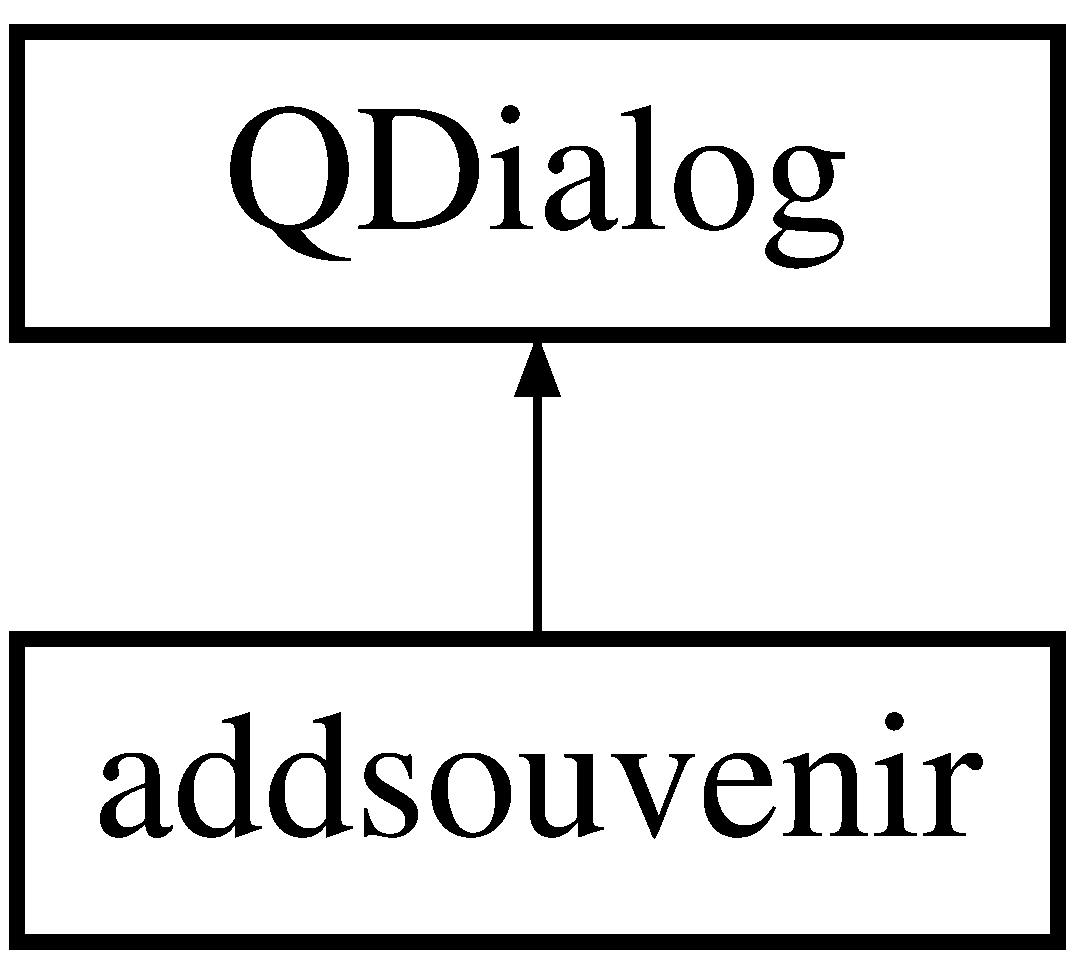
\includegraphics[height=2.000000cm]{classaddsouvenir}
\end{center}
\end{figure}
\subsection*{Signals}
\begin{DoxyCompactItemize}
\item 
void \hyperlink{classaddsouvenir_a4075c8409ec8fe021609d8eedc7e316e}{refresh\+Models} ()
\end{DoxyCompactItemize}
\subsection*{Public Member Functions}
\begin{DoxyCompactItemize}
\item 
\hyperlink{classaddsouvenir_a9c6589d61f31a2bcae2ba6f439b19f20}{addsouvenir} (Q\+Widget $\ast$parent=0, \hyperlink{class_database}{Database} $\ast$db=0, Q\+String stadium\+Name=\char`\"{}null\char`\"{})
\item 
\hyperlink{classaddsouvenir_ad8a758c4ee2056d4b3847a4635810c4e}{$\sim$addsouvenir} ()
\end{DoxyCompactItemize}


\subsection{Detailed Description}


Definition at line 11 of file addsouvenir.\+h.



\subsection{Constructor \& Destructor Documentation}
\index{addsouvenir@{addsouvenir}!addsouvenir@{addsouvenir}}
\index{addsouvenir@{addsouvenir}!addsouvenir@{addsouvenir}}
\subsubsection[{\texorpdfstring{addsouvenir(\+Q\+Widget $\ast$parent=0, Database $\ast$db=0, Q\+String stadium\+Name=""null"")}{addsouvenir(QWidget *parent=0, Database *db=0, QString stadiumName="null")}}]{\setlength{\rightskip}{0pt plus 5cm}addsouvenir\+::addsouvenir (
\begin{DoxyParamCaption}
\item[{Q\+Widget $\ast$}]{parent = {\ttfamily 0}, }
\item[{{\bf Database} $\ast$}]{db = {\ttfamily 0}, }
\item[{Q\+String}]{stadium\+Name = {\ttfamily \char`\"{}null\char`\"{}}}
\end{DoxyParamCaption}
)\hspace{0.3cm}{\ttfamily [explicit]}}\hypertarget{classaddsouvenir_a9c6589d61f31a2bcae2ba6f439b19f20}{}\label{classaddsouvenir_a9c6589d61f31a2bcae2ba6f439b19f20}


Definition at line 4 of file addsouvenir.\+cpp.

\index{addsouvenir@{addsouvenir}!````~addsouvenir@{$\sim$addsouvenir}}
\index{````~addsouvenir@{$\sim$addsouvenir}!addsouvenir@{addsouvenir}}
\subsubsection[{\texorpdfstring{$\sim$addsouvenir()}{~addsouvenir()}}]{\setlength{\rightskip}{0pt plus 5cm}addsouvenir\+::$\sim$addsouvenir (
\begin{DoxyParamCaption}
{}
\end{DoxyParamCaption}
)}\hypertarget{classaddsouvenir_ad8a758c4ee2056d4b3847a4635810c4e}{}\label{classaddsouvenir_ad8a758c4ee2056d4b3847a4635810c4e}


Definition at line 14 of file addsouvenir.\+cpp.



\subsection{Member Function Documentation}
\index{addsouvenir@{addsouvenir}!refresh\+Models@{refresh\+Models}}
\index{refresh\+Models@{refresh\+Models}!addsouvenir@{addsouvenir}}
\subsubsection[{\texorpdfstring{refresh\+Models}{refreshModels}}]{\setlength{\rightskip}{0pt plus 5cm}void addsouvenir\+::refresh\+Models (
\begin{DoxyParamCaption}
{}
\end{DoxyParamCaption}
)\hspace{0.3cm}{\ttfamily [signal]}}\hypertarget{classaddsouvenir_a4075c8409ec8fe021609d8eedc7e316e}{}\label{classaddsouvenir_a4075c8409ec8fe021609d8eedc7e316e}


The documentation for this class was generated from the following files\+:\begin{DoxyCompactItemize}
\item 
src/header/\hyperlink{addsouvenir_8h}{addsouvenir.\+h}\item 
src/source/\hyperlink{addsouvenir_8cpp}{addsouvenir.\+cpp}\end{DoxyCompactItemize}

\hypertarget{class_admin_login}{}\section{Admin\+Login Class Reference}
\label{class_admin_login}\index{Admin\+Login@{Admin\+Login}}


{\ttfamily \#include $<$adminlogin.\+h$>$}

Inheritance diagram for Admin\+Login\+:\begin{figure}[H]
\begin{center}
\leavevmode
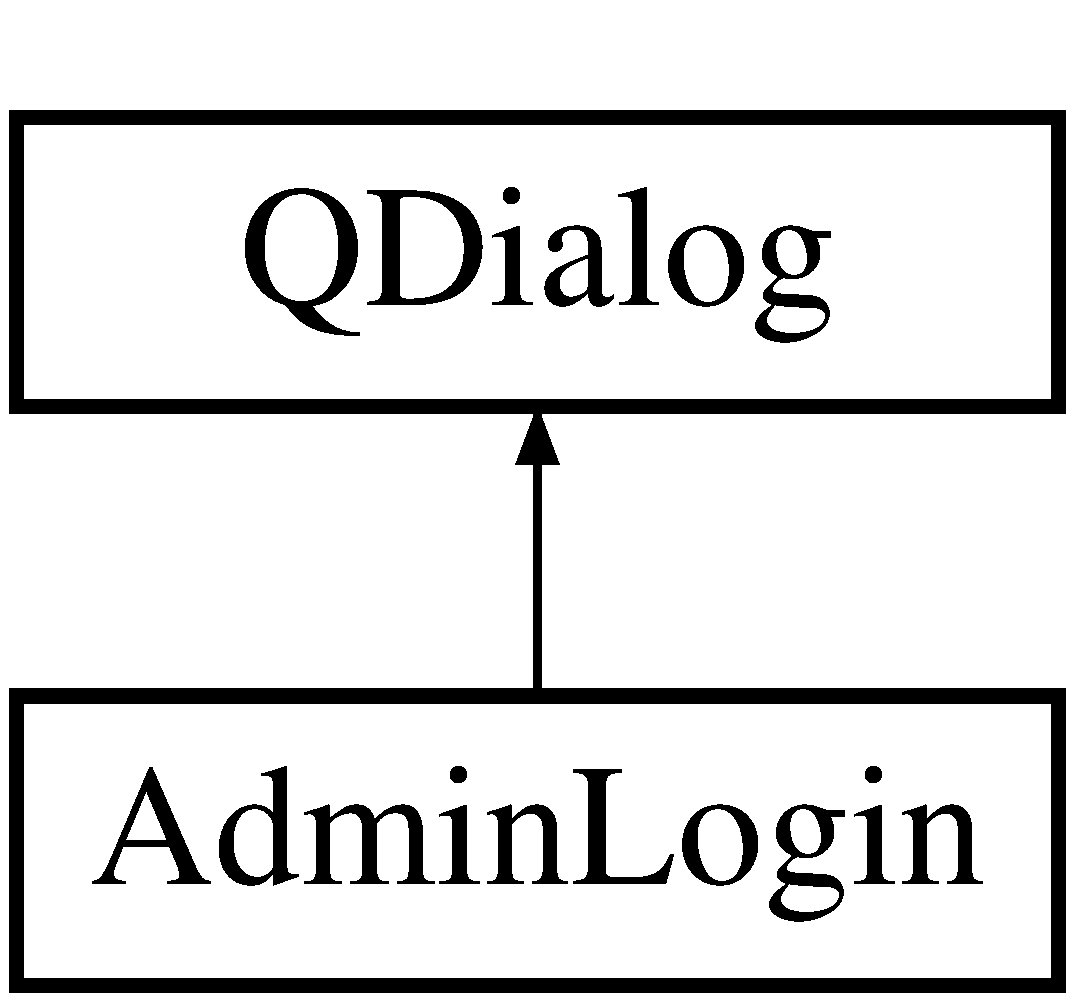
\includegraphics[height=2.000000cm]{class_admin_login}
\end{center}
\end{figure}
\subsection*{Signals}
\begin{DoxyCompactItemize}
\item 
void \hyperlink{class_admin_login_a1a60601c7f53660082780201c1b25b20}{admin\+Status\+Changed} (bool status)
\end{DoxyCompactItemize}
\subsection*{Public Member Functions}
\begin{DoxyCompactItemize}
\item 
\hyperlink{class_admin_login_a3e1c90c550d6d7abf2a58c4919e80461}{Admin\+Login} (Q\+Widget $\ast$parent=0)
\item 
\hyperlink{class_admin_login_a72502ef239f57ca69fa54d3c94c07985}{$\sim$\+Admin\+Login} ()
\end{DoxyCompactItemize}


\subsection{Detailed Description}


Definition at line 13 of file adminlogin.\+h.



\subsection{Constructor \& Destructor Documentation}
\index{Admin\+Login@{Admin\+Login}!Admin\+Login@{Admin\+Login}}
\index{Admin\+Login@{Admin\+Login}!Admin\+Login@{Admin\+Login}}
\subsubsection[{\texorpdfstring{Admin\+Login(\+Q\+Widget $\ast$parent=0)}{AdminLogin(QWidget *parent=0)}}]{\setlength{\rightskip}{0pt plus 5cm}Admin\+Login\+::\+Admin\+Login (
\begin{DoxyParamCaption}
\item[{Q\+Widget $\ast$}]{parent = {\ttfamily 0}}
\end{DoxyParamCaption}
)\hspace{0.3cm}{\ttfamily [explicit]}}\hypertarget{class_admin_login_a3e1c90c550d6d7abf2a58c4919e80461}{}\label{class_admin_login_a3e1c90c550d6d7abf2a58c4919e80461}


Definition at line 4 of file adminlogin.\+cpp.

\index{Admin\+Login@{Admin\+Login}!````~Admin\+Login@{$\sim$\+Admin\+Login}}
\index{````~Admin\+Login@{$\sim$\+Admin\+Login}!Admin\+Login@{Admin\+Login}}
\subsubsection[{\texorpdfstring{$\sim$\+Admin\+Login()}{~AdminLogin()}}]{\setlength{\rightskip}{0pt plus 5cm}Admin\+Login\+::$\sim$\+Admin\+Login (
\begin{DoxyParamCaption}
{}
\end{DoxyParamCaption}
)}\hypertarget{class_admin_login_a72502ef239f57ca69fa54d3c94c07985}{}\label{class_admin_login_a72502ef239f57ca69fa54d3c94c07985}


Definition at line 13 of file adminlogin.\+cpp.



\subsection{Member Function Documentation}
\index{Admin\+Login@{Admin\+Login}!admin\+Status\+Changed@{admin\+Status\+Changed}}
\index{admin\+Status\+Changed@{admin\+Status\+Changed}!Admin\+Login@{Admin\+Login}}
\subsubsection[{\texorpdfstring{admin\+Status\+Changed}{adminStatusChanged}}]{\setlength{\rightskip}{0pt plus 5cm}void Admin\+Login\+::admin\+Status\+Changed (
\begin{DoxyParamCaption}
\item[{bool}]{status}
\end{DoxyParamCaption}
)\hspace{0.3cm}{\ttfamily [signal]}}\hypertarget{class_admin_login_a1a60601c7f53660082780201c1b25b20}{}\label{class_admin_login_a1a60601c7f53660082780201c1b25b20}


The documentation for this class was generated from the following files\+:\begin{DoxyCompactItemize}
\item 
src/header/\hyperlink{adminlogin_8h}{adminlogin.\+h}\item 
src/source/\hyperlink{adminlogin_8cpp}{adminlogin.\+cpp}\end{DoxyCompactItemize}

\hypertarget{struct_q_list_data_1_1_array_compatible_layout}{}\section{Q\+List\+Data\+:\+:Array\+Compatible\+Layout Struct Reference}
\label{struct_q_list_data_1_1_array_compatible_layout}\index{Q\+List\+Data\+::\+Array\+Compatible\+Layout@{Q\+List\+Data\+::\+Array\+Compatible\+Layout}}


{\ttfamily \#include $<$qlist.\+h$>$}

Inheritance diagram for Q\+List\+Data\+:\+:Array\+Compatible\+Layout\+:\begin{figure}[H]
\begin{center}
\leavevmode
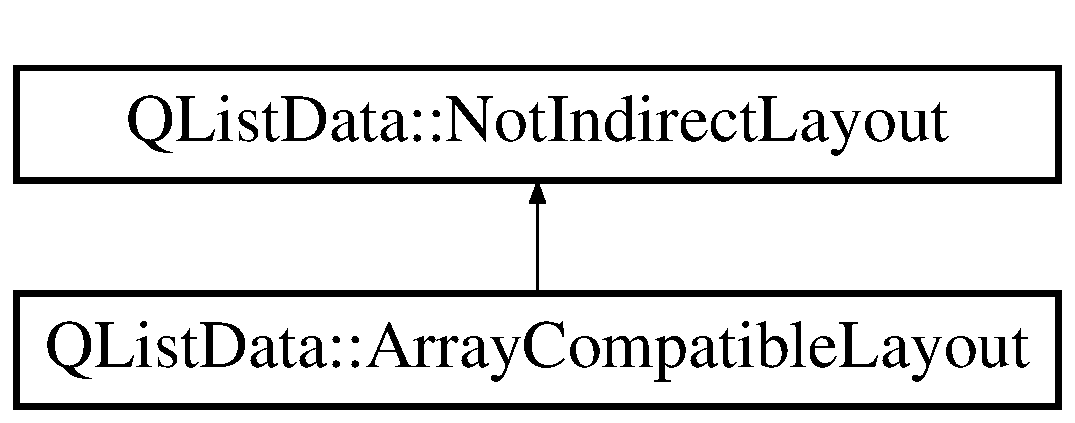
\includegraphics[height=2.000000cm]{struct_q_list_data_1_1_array_compatible_layout}
\end{center}
\end{figure}


\subsection{Detailed Description}


Definition at line 78 of file qlist.\+h.



The documentation for this struct was generated from the following file\+:\begin{DoxyCompactItemize}
\item 
docs/extra-\/files/\hyperlink{qlist_8h}{qlist.\+h}\end{DoxyCompactItemize}

\hypertarget{structcomp}{}\section{comp Struct Reference}
\label{structcomp}\index{comp@{comp}}


The comp struct Comparator struct used for comparing the weights of two edges.  




{\ttfamily \#include $<$vertex.\+h$>$}

\subsection*{Public Member Functions}
\begin{DoxyCompactItemize}
\item 
bool \hyperlink{structcomp_a4474ff972985ad9bdeb96412b287cdb4}{operator()} (const \hyperlink{struct_edge}{Edge} \&e1, const \hyperlink{struct_edge}{Edge} \&e2) const 
\end{DoxyCompactItemize}


\subsection{Detailed Description}
The comp struct Comparator struct used for comparing the weights of two edges. 

Definition at line 20 of file vertex.\+h.



\subsection{Member Function Documentation}
\index{comp@{comp}!operator()@{operator()}}
\index{operator()@{operator()}!comp@{comp}}
\subsubsection[{\texorpdfstring{operator()(const Edge \&e1, const Edge \&e2) const }{operator()(const Edge &e1, const Edge &e2) const }}]{\setlength{\rightskip}{0pt plus 5cm}bool comp\+::operator() (
\begin{DoxyParamCaption}
\item[{const {\bf Edge} \&}]{e1, }
\item[{const {\bf Edge} \&}]{e2}
\end{DoxyParamCaption}
) const\hspace{0.3cm}{\ttfamily [inline]}}\hypertarget{structcomp_a4474ff972985ad9bdeb96412b287cdb4}{}\label{structcomp_a4474ff972985ad9bdeb96412b287cdb4}


Definition at line 22 of file vertex.\+h.



The documentation for this struct was generated from the following file\+:\begin{DoxyCompactItemize}
\item 
src/header/\hyperlink{vertex_8h}{vertex.\+h}\end{DoxyCompactItemize}

\hypertarget{class_q_list_1_1const__iterator}{}\section{Q\+List$<$ T $>$\+:\+:const\+\_\+iterator Class Reference}
\label{class_q_list_1_1const__iterator}\index{Q\+List$<$ T $>$\+::const\+\_\+iterator@{Q\+List$<$ T $>$\+::const\+\_\+iterator}}


The \hyperlink{class_q_list_1_1const__iterator}{Q\+List\+::const\+\_\+iterator} class provides an S\+T\+L-\/style const iterator for \hyperlink{class_q_list}{Q\+List} and Q\+Queue.  




{\ttfamily \#include $<$qlist.\+h$>$}

\subsection*{Public Types}
\begin{DoxyCompactItemize}
\item 
typedef std\+::random\+\_\+access\+\_\+iterator\+\_\+tag \hyperlink{class_q_list_1_1const__iterator_a3f60c0d419aa760c74baf9259c5309a7}{iterator\+\_\+category}
\item 
typedef qptrdiff \hyperlink{class_q_list_1_1const__iterator_a3fd13f34a4cad0b55bff738b349a87c6}{difference\+\_\+type}
\item 
typedef T \hyperlink{class_q_list_1_1const__iterator_a47f4f5c7fa5edd61cf19a5dde299c588}{value\+\_\+type}
\item 
typedef const T $\ast$ \hyperlink{class_q_list_1_1const__iterator_a533c6c850de0bc2484878d5c4bcb0513}{pointer}
\item 
typedef const T \& \hyperlink{class_q_list_1_1const__iterator_a52b9df9ae3c6d68e3b34cc0430e782e6}{reference}
\end{DoxyCompactItemize}
\subsection*{Public Member Functions}
\begin{DoxyCompactItemize}
\item 
\hyperlink{class_q_list_1_1const__iterator_afe91d91a7946da54e2e07ffed0e8f5f5}{const\+\_\+iterator} ()
\item 
\hyperlink{class_q_list_1_1const__iterator_ac38ce73f4abe9cdbf7d7c2a0a6f5af12}{const\+\_\+iterator} (Node $\ast$n)
\item 
\hyperlink{class_q_list_1_1const__iterator_a1fac43c70d34ac46e680ec03072c3107}{const\+\_\+iterator} (const \hyperlink{class_q_list_1_1const__iterator}{const\+\_\+iterator} \&o)
\item 
\hyperlink{class_q_list_1_1const__iterator_a7564cc84899e520dcc3be05c7ab6a7be}{const\+\_\+iterator} (const \hyperlink{class_q_list_1_1iterator}{iterator} \&o)
\item 
const T \& \hyperlink{class_q_list_1_1const__iterator_ae8ba811eff602158dc96bb4091069839}{operator$\ast$} () const 
\item 
const T $\ast$ \hyperlink{class_q_list_1_1const__iterator_ae4d16b861e178013e71ee231a4a5f6e6}{operator-\/$>$} () const 
\item 
const T \& \hyperlink{class_q_list_1_1const__iterator_a0bc2c77f62a523b99897b7d9d46ec9ce}{operator\mbox{[}$\,$\mbox{]}} (\hyperlink{class_q_list_1_1const__iterator_a3fd13f34a4cad0b55bff738b349a87c6}{difference\+\_\+type} j) const 
\item 
bool \hyperlink{class_q_list_1_1const__iterator_afcc84c3f71a5a747a2323b11eee25a33}{operator==} (const \hyperlink{class_q_list_1_1const__iterator}{const\+\_\+iterator} \&o) const 
\item 
bool \hyperlink{class_q_list_1_1const__iterator_a3fed9135a0637f7057d41d7a29be7528}{operator!=} (const \hyperlink{class_q_list_1_1const__iterator}{const\+\_\+iterator} \&o) const 
\item 
bool \hyperlink{class_q_list_1_1const__iterator_a9da50890a3ecb341646c7f0b884dd75f}{operator$<$} (const \hyperlink{class_q_list_1_1const__iterator}{const\+\_\+iterator} \&other) const 
\item 
bool \hyperlink{class_q_list_1_1const__iterator_ae7f68657a78b318d3a9b11566f2755aa}{operator$<$=} (const \hyperlink{class_q_list_1_1const__iterator}{const\+\_\+iterator} \&other) const 
\item 
bool \hyperlink{class_q_list_1_1const__iterator_aba039471e2636c49e3ccf31966ee2cf6}{operator$>$} (const \hyperlink{class_q_list_1_1const__iterator}{const\+\_\+iterator} \&other) const 
\item 
bool \hyperlink{class_q_list_1_1const__iterator_aab6f2d1a5b1d0a313580123be000d0bb}{operator$>$=} (const \hyperlink{class_q_list_1_1const__iterator}{const\+\_\+iterator} \&other) const 
\item 
\hyperlink{class_q_list_1_1const__iterator}{const\+\_\+iterator} \& \hyperlink{class_q_list_1_1const__iterator_a429a8e3aa3de97b20c59f0a8524c94d9}{operator++} ()
\item 
\hyperlink{class_q_list_1_1const__iterator}{const\+\_\+iterator} \hyperlink{class_q_list_1_1const__iterator_ad040d3871a716a76f1b57705fb666bd5}{operator++} (int)
\item 
\hyperlink{class_q_list_1_1const__iterator}{const\+\_\+iterator} \& \hyperlink{class_q_list_1_1const__iterator_ac84c629637f34370020d66afc3a2a2cf}{operator-\/-\/} ()
\item 
\hyperlink{class_q_list_1_1const__iterator}{const\+\_\+iterator} \hyperlink{class_q_list_1_1const__iterator_a46d687d497d7aa49e5b65d52d3b4eb20}{operator-\/-\/} (int)
\item 
\hyperlink{class_q_list_1_1const__iterator}{const\+\_\+iterator} \& \hyperlink{class_q_list_1_1const__iterator_afe9c88b39e111149d46cddc4a4caf445}{operator+=} (\hyperlink{class_q_list_1_1const__iterator_a3fd13f34a4cad0b55bff738b349a87c6}{difference\+\_\+type} j)
\item 
\hyperlink{class_q_list_1_1const__iterator}{const\+\_\+iterator} \& \hyperlink{class_q_list_1_1const__iterator_a4a975b8077a87db810d6cb3606e23558}{operator-\/=} (\hyperlink{class_q_list_1_1const__iterator_a3fd13f34a4cad0b55bff738b349a87c6}{difference\+\_\+type} j)
\item 
\hyperlink{class_q_list_1_1const__iterator}{const\+\_\+iterator} \hyperlink{class_q_list_1_1const__iterator_a38269688da0773c04e5207ab9828f965}{operator+} (\hyperlink{class_q_list_1_1const__iterator_a3fd13f34a4cad0b55bff738b349a87c6}{difference\+\_\+type} j) const 
\item 
\hyperlink{class_q_list_1_1const__iterator}{const\+\_\+iterator} \hyperlink{class_q_list_1_1const__iterator_a15eef6f9c016b44cebdc748d35a25f05}{operator-\/} (\hyperlink{class_q_list_1_1const__iterator_a3fd13f34a4cad0b55bff738b349a87c6}{difference\+\_\+type} j) const 
\item 
int \hyperlink{class_q_list_1_1const__iterator_ad67a8f57c648efb3675f8cb9f3dc7d00}{operator-\/} (\hyperlink{class_q_list_1_1const__iterator}{const\+\_\+iterator} j) const 
\end{DoxyCompactItemize}
\subsection*{Public Attributes}
\begin{DoxyCompactItemize}
\item 
Node $\ast$ \hyperlink{class_q_list_1_1const__iterator_aaf98a66ebc335c3f611550ce99c1406c}{i}
\end{DoxyCompactItemize}


\subsection{Detailed Description}
\subsubsection*{template$<$typename T$>$\\*
class Q\+List$<$ T $>$\+::const\+\_\+iterator}

The \hyperlink{class_q_list_1_1const__iterator}{Q\+List\+::const\+\_\+iterator} class provides an S\+T\+L-\/style const iterator for \hyperlink{class_q_list}{Q\+List} and Q\+Queue. 

Qt\+Core \hyperlink{class_q_list}{Q\+List} provides both \{S\+T\+L-\/style iterators\} and \{Java-\/style iterators\}. The S\+T\+L-\/style iterators are more low-\/level and more cumbersome to use; on the other hand, they are slightly faster and, for developers who already know S\+TL, have the advantage of familiarity.

\hyperlink{class_q_list}{Q\+List}$<$T$>$\+::const\+\_\+iterator allows you to iterate over a \hyperlink{class_q_list}{Q\+List}$<$T$>$ (or a Q\+Queue$<$T$>$). If you want to modify the \hyperlink{class_q_list}{Q\+List} as you iterate over it, use \hyperlink{class_q_list_1_1iterator}{Q\+List\+::iterator} instead. It is generally good practice to use \hyperlink{class_q_list_1_1const__iterator}{Q\+List\+::const\+\_\+iterator} on a non-\/const \hyperlink{class_q_list}{Q\+List} as well, unless you need to change the \hyperlink{class_q_list}{Q\+List} through the iterator. Const iterators are slightly faster, and can improve code readability.

The default \hyperlink{class_q_list_1_1const__iterator}{Q\+List\+::const\+\_\+iterator} constructor creates an uninitialized iterator. You must initialize it using a \hyperlink{class_q_list}{Q\+List} function like \hyperlink{class_q_list_a8f6d53fe01e1c2aaea0a446580f99cdb}{Q\+List\+::const\+Begin()}, \hyperlink{class_q_list_a66e34d5df478dda9190b9b075317690d}{Q\+List\+::const\+End()}, or \hyperlink{class_q_list_a2ae4b66fdb5875c4c55eb903fa5ca25b}{Q\+List\+::insert()} before you can start iterating. Here\textquotesingle{}s a typical loop that prints all the items stored in a list\+:


\begin{DoxyCodeInclude}
\end{DoxyCodeInclude}
 Most \hyperlink{class_q_list}{Q\+List} functions accept an integer index rather than an iterator. For that reason, iterators are rarely useful in connection with \hyperlink{class_q_list}{Q\+List}. One place where S\+T\+L-\/style iterators do make sense is as arguments to \{generic algorithms\}.

For example, here\textquotesingle{}s how to delete all the widgets stored in a \hyperlink{class_q_list}{Q\+List}$<$Q\+Widget $\ast$$>$\+:


\begin{DoxyCodeInclude}
\end{DoxyCodeInclude}
 Multiple iterators can be used on the same list. However, be aware that any non-\/const function call performed on the \hyperlink{class_q_list}{Q\+List} will render all existing iterators undefined. If you need to keep iterators over a long period of time, we recommend that you use Q\+Linked\+List rather than \hyperlink{class_q_list}{Q\+List}.

\begin{DoxyWarning}{Warning}
Iterators on implicitly shared containers do not work exactly like S\+T\+L-\/iterators. You should avoid copying a container while iterators are active on that container. For more information, read \{Implicit sharing iterator problem\}.
\end{DoxyWarning}
\begin{DoxySeeAlso}{See also}
\hyperlink{class_q_list_1_1iterator}{Q\+List\+::iterator}, Q\+List\+Iterator 
\end{DoxySeeAlso}


Definition at line 259 of file qlist.\+h.



\subsection{Member Typedef Documentation}
\index{Q\+List\+::const\+\_\+iterator@{Q\+List\+::const\+\_\+iterator}!difference\+\_\+type@{difference\+\_\+type}}
\index{difference\+\_\+type@{difference\+\_\+type}!Q\+List\+::const\+\_\+iterator@{Q\+List\+::const\+\_\+iterator}}
\subsubsection[{\texorpdfstring{difference\+\_\+type}{difference_type}}]{\setlength{\rightskip}{0pt plus 5cm}template$<$typename T$>$ {\bf Q\+List}$<$ T $>$\+::{\bf const\+\_\+iterator\+::difference\+\_\+type}}\hypertarget{class_q_list_1_1const__iterator_a3fd13f34a4cad0b55bff738b349a87c6}{}\label{class_q_list_1_1const__iterator_a3fd13f34a4cad0b55bff738b349a87c6}


Definition at line 264 of file qlist.\+h.

\index{Q\+List\+::const\+\_\+iterator@{Q\+List\+::const\+\_\+iterator}!iterator\+\_\+category@{iterator\+\_\+category}}
\index{iterator\+\_\+category@{iterator\+\_\+category}!Q\+List\+::const\+\_\+iterator@{Q\+List\+::const\+\_\+iterator}}
\subsubsection[{\texorpdfstring{iterator\+\_\+category}{iterator_category}}]{\setlength{\rightskip}{0pt plus 5cm}template$<$typename T$>$ {\bf Q\+List}$<$ T $>$\+::{\bf const\+\_\+iterator\+::iterator\+\_\+category}}\hypertarget{class_q_list_1_1const__iterator_a3f60c0d419aa760c74baf9259c5309a7}{}\label{class_q_list_1_1const__iterator_a3f60c0d419aa760c74baf9259c5309a7}
A synonym for {\itshape \{std\+::random\+\_\+access\+\_\+iterator\+\_\+tag\}} indicating this iterator is a random access iterator. 

Definition at line 262 of file qlist.\+h.

\index{Q\+List\+::const\+\_\+iterator@{Q\+List\+::const\+\_\+iterator}!pointer@{pointer}}
\index{pointer@{pointer}!Q\+List\+::const\+\_\+iterator@{Q\+List\+::const\+\_\+iterator}}
\subsubsection[{\texorpdfstring{pointer}{pointer}}]{\setlength{\rightskip}{0pt plus 5cm}template$<$typename T$>$ {\bf Q\+List}$<$ T $>$\+::{\bf const\+\_\+iterator\+::pointer}}\hypertarget{class_q_list_1_1const__iterator_a533c6c850de0bc2484878d5c4bcb0513}{}\label{class_q_list_1_1const__iterator_a533c6c850de0bc2484878d5c4bcb0513}


Definition at line 266 of file qlist.\+h.

\index{Q\+List\+::const\+\_\+iterator@{Q\+List\+::const\+\_\+iterator}!reference@{reference}}
\index{reference@{reference}!Q\+List\+::const\+\_\+iterator@{Q\+List\+::const\+\_\+iterator}}
\subsubsection[{\texorpdfstring{reference}{reference}}]{\setlength{\rightskip}{0pt plus 5cm}template$<$typename T$>$ {\bf Q\+List}$<$ T $>$\+::{\bf const\+\_\+iterator\+::reference}}\hypertarget{class_q_list_1_1const__iterator_a52b9df9ae3c6d68e3b34cc0430e782e6}{}\label{class_q_list_1_1const__iterator_a52b9df9ae3c6d68e3b34cc0430e782e6}


Definition at line 267 of file qlist.\+h.

\index{Q\+List\+::const\+\_\+iterator@{Q\+List\+::const\+\_\+iterator}!value\+\_\+type@{value\+\_\+type}}
\index{value\+\_\+type@{value\+\_\+type}!Q\+List\+::const\+\_\+iterator@{Q\+List\+::const\+\_\+iterator}}
\subsubsection[{\texorpdfstring{value\+\_\+type}{value_type}}]{\setlength{\rightskip}{0pt plus 5cm}template$<$typename T$>$ {\bf Q\+List}$<$ T $>$\+::{\bf const\+\_\+iterator\+::value\+\_\+type}}\hypertarget{class_q_list_1_1const__iterator_a47f4f5c7fa5edd61cf19a5dde299c588}{}\label{class_q_list_1_1const__iterator_a47f4f5c7fa5edd61cf19a5dde299c588}


Definition at line 265 of file qlist.\+h.



\subsection{Constructor \& Destructor Documentation}
\index{Q\+List\+::const\+\_\+iterator@{Q\+List\+::const\+\_\+iterator}!const\+\_\+iterator@{const\+\_\+iterator}}
\index{const\+\_\+iterator@{const\+\_\+iterator}!Q\+List\+::const\+\_\+iterator@{Q\+List\+::const\+\_\+iterator}}
\subsubsection[{\texorpdfstring{const\+\_\+iterator()}{const_iterator()}}]{\setlength{\rightskip}{0pt plus 5cm}template$<$typename T$>$ {\bf Q\+List}$<$ T $>$\+::const\+\_\+iterator\+::const\+\_\+iterator (
\begin{DoxyParamCaption}
{}
\end{DoxyParamCaption}
)\hspace{0.3cm}{\ttfamily [inline]}}\hypertarget{class_q_list_1_1const__iterator_afe91d91a7946da54e2e07ffed0e8f5f5}{}\label{class_q_list_1_1const__iterator_afe91d91a7946da54e2e07ffed0e8f5f5}
Constructs an uninitialized iterator.

Functions like \hyperlink{class_q_list_1_1const__iterator_ae8ba811eff602158dc96bb4091069839}{operator$\ast$()} and \hyperlink{class_q_list_1_1const__iterator_a429a8e3aa3de97b20c59f0a8524c94d9}{operator++()} should not be called on an uninitialized iterator. Use \hyperlink{class_q_list_af210d61c252a7f0124854a9fea8fc23d}{operator=()} to assign a value to it before using it.

\begin{DoxySeeAlso}{See also}
\hyperlink{class_q_list_a8f6d53fe01e1c2aaea0a446580f99cdb}{Q\+List\+::const\+Begin()}, \hyperlink{class_q_list_a66e34d5df478dda9190b9b075317690d}{Q\+List\+::const\+End()} 
\end{DoxySeeAlso}


Definition at line 269 of file qlist.\+h.

\index{Q\+List\+::const\+\_\+iterator@{Q\+List\+::const\+\_\+iterator}!const\+\_\+iterator@{const\+\_\+iterator}}
\index{const\+\_\+iterator@{const\+\_\+iterator}!Q\+List\+::const\+\_\+iterator@{Q\+List\+::const\+\_\+iterator}}
\subsubsection[{\texorpdfstring{const\+\_\+iterator(\+Node $\ast$n)}{const_iterator(Node *n)}}]{\setlength{\rightskip}{0pt plus 5cm}template$<$typename T$>$ {\bf Q\+List}$<$ T $>$\+::const\+\_\+iterator\+::const\+\_\+iterator (
\begin{DoxyParamCaption}
\item[{Node $\ast$}]{n}
\end{DoxyParamCaption}
)\hspace{0.3cm}{\ttfamily [inline]}}\hypertarget{class_q_list_1_1const__iterator_ac38ce73f4abe9cdbf7d7c2a0a6f5af12}{}\label{class_q_list_1_1const__iterator_ac38ce73f4abe9cdbf7d7c2a0a6f5af12}


Definition at line 270 of file qlist.\+h.

\index{Q\+List\+::const\+\_\+iterator@{Q\+List\+::const\+\_\+iterator}!const\+\_\+iterator@{const\+\_\+iterator}}
\index{const\+\_\+iterator@{const\+\_\+iterator}!Q\+List\+::const\+\_\+iterator@{Q\+List\+::const\+\_\+iterator}}
\subsubsection[{\texorpdfstring{const\+\_\+iterator(const const\+\_\+iterator \&o)}{const_iterator(const const_iterator &o)}}]{\setlength{\rightskip}{0pt plus 5cm}template$<$typename T$>$ {\bf Q\+List}$<$ T $>$\+::const\+\_\+iterator\+::const\+\_\+iterator (
\begin{DoxyParamCaption}
\item[{const {\bf const\+\_\+iterator} \&}]{other}
\end{DoxyParamCaption}
)\hspace{0.3cm}{\ttfamily [inline]}}\hypertarget{class_q_list_1_1const__iterator_a1fac43c70d34ac46e680ec03072c3107}{}\label{class_q_list_1_1const__iterator_a1fac43c70d34ac46e680ec03072c3107}
Constructs a copy of {\itshape other}. 

Definition at line 271 of file qlist.\+h.

\index{Q\+List\+::const\+\_\+iterator@{Q\+List\+::const\+\_\+iterator}!const\+\_\+iterator@{const\+\_\+iterator}}
\index{const\+\_\+iterator@{const\+\_\+iterator}!Q\+List\+::const\+\_\+iterator@{Q\+List\+::const\+\_\+iterator}}
\subsubsection[{\texorpdfstring{const\+\_\+iterator(const iterator \&o)}{const_iterator(const iterator &o)}}]{\setlength{\rightskip}{0pt plus 5cm}template$<$typename T$>$ {\bf Q\+List}$<$ T $>$\+::const\+\_\+iterator\+::const\+\_\+iterator (
\begin{DoxyParamCaption}
\item[{const {\bf iterator} \&}]{other}
\end{DoxyParamCaption}
)\hspace{0.3cm}{\ttfamily [inline]}}\hypertarget{class_q_list_1_1const__iterator_a7564cc84899e520dcc3be05c7ab6a7be}{}\label{class_q_list_1_1const__iterator_a7564cc84899e520dcc3be05c7ab6a7be}
Constructs a copy of {\itshape other}. 

Definition at line 275 of file qlist.\+h.



\subsection{Member Function Documentation}
\index{Q\+List\+::const\+\_\+iterator@{Q\+List\+::const\+\_\+iterator}!operator"!=@{operator"!=}}
\index{operator"!=@{operator"!=}!Q\+List\+::const\+\_\+iterator@{Q\+List\+::const\+\_\+iterator}}
\subsubsection[{\texorpdfstring{operator"!=(const const\+\_\+iterator \&o) const }{operator!=(const const_iterator &o) const }}]{\setlength{\rightskip}{0pt plus 5cm}template$<$typename T$>$ bool {\bf Q\+List}$<$ T $>$\+::const\+\_\+iterator\+::operator!= (
\begin{DoxyParamCaption}
\item[{const {\bf const\+\_\+iterator} \&}]{other}
\end{DoxyParamCaption}
) const\hspace{0.3cm}{\ttfamily [inline]}}\hypertarget{class_q_list_1_1const__iterator_a3fed9135a0637f7057d41d7a29be7528}{}\label{class_q_list_1_1const__iterator_a3fed9135a0637f7057d41d7a29be7528}
Returns {\ttfamily true} if {\itshape other} points to a different item than this iterator; otherwise returns {\ttfamily false}.

\begin{DoxySeeAlso}{See also}
\hyperlink{class_q_list_1_1const__iterator_afcc84c3f71a5a747a2323b11eee25a33}{operator==()} 
\end{DoxySeeAlso}


Definition at line 281 of file qlist.\+h.

\index{Q\+List\+::const\+\_\+iterator@{Q\+List\+::const\+\_\+iterator}!operator$\ast$@{operator$\ast$}}
\index{operator$\ast$@{operator$\ast$}!Q\+List\+::const\+\_\+iterator@{Q\+List\+::const\+\_\+iterator}}
\subsubsection[{\texorpdfstring{operator$\ast$() const }{operator*() const }}]{\setlength{\rightskip}{0pt plus 5cm}template$<$typename T$>$ const T \& {\bf Q\+List}$<$ T $>$\+::const\+\_\+iterator\+::operator$\ast$ (
\begin{DoxyParamCaption}
{}
\end{DoxyParamCaption}
) const\hspace{0.3cm}{\ttfamily [inline]}}\hypertarget{class_q_list_1_1const__iterator_ae8ba811eff602158dc96bb4091069839}{}\label{class_q_list_1_1const__iterator_ae8ba811eff602158dc96bb4091069839}
Returns the current item.

\begin{DoxySeeAlso}{See also}
\hyperlink{class_q_list_1_1const__iterator_ae4d16b861e178013e71ee231a4a5f6e6}{operator-\/$>$()} 
\end{DoxySeeAlso}


Definition at line 277 of file qlist.\+h.

\index{Q\+List\+::const\+\_\+iterator@{Q\+List\+::const\+\_\+iterator}!operator+@{operator+}}
\index{operator+@{operator+}!Q\+List\+::const\+\_\+iterator@{Q\+List\+::const\+\_\+iterator}}
\subsubsection[{\texorpdfstring{operator+(difference\+\_\+type j) const }{operator+(difference_type j) const }}]{\setlength{\rightskip}{0pt plus 5cm}template$<$typename T$>$ {\bf Q\+List\+::const\+\_\+iterator} {\bf Q\+List}$<$ T $>$\+::const\+\_\+iterator\+::operator+ (
\begin{DoxyParamCaption}
\item[{{\bf difference\+\_\+type}}]{j}
\end{DoxyParamCaption}
) const\hspace{0.3cm}{\ttfamily [inline]}}\hypertarget{class_q_list_1_1const__iterator_a38269688da0773c04e5207ab9828f965}{}\label{class_q_list_1_1const__iterator_a38269688da0773c04e5207ab9828f965}
Returns an iterator to the item at {\itshape j} positions forward from this iterator. (If {\itshape j} is negative, the iterator goes backward.)

\begin{DoxySeeAlso}{See also}
\hyperlink{class_q_list_1_1const__iterator_a15eef6f9c016b44cebdc748d35a25f05}{operator-\/()}, \hyperlink{class_q_list_1_1const__iterator_afe9c88b39e111149d46cddc4a4caf445}{operator+=()} 
\end{DoxySeeAlso}


Definition at line 292 of file qlist.\+h.

\index{Q\+List\+::const\+\_\+iterator@{Q\+List\+::const\+\_\+iterator}!operator++@{operator++}}
\index{operator++@{operator++}!Q\+List\+::const\+\_\+iterator@{Q\+List\+::const\+\_\+iterator}}
\subsubsection[{\texorpdfstring{operator++()}{operator++()}}]{\setlength{\rightskip}{0pt plus 5cm}template$<$typename T$>$ {\bf Q\+List\+::const\+\_\+iterator} \& {\bf Q\+List}$<$ T $>$\+::const\+\_\+iterator\+::operator++ (
\begin{DoxyParamCaption}
{}
\end{DoxyParamCaption}
)\hspace{0.3cm}{\ttfamily [inline]}}\hypertarget{class_q_list_1_1const__iterator_a429a8e3aa3de97b20c59f0a8524c94d9}{}\label{class_q_list_1_1const__iterator_a429a8e3aa3de97b20c59f0a8524c94d9}
The prefix ++ operator ({\ttfamily }\{++it\}) advances the iterator to the next item in the list and returns an iterator to the new current item.

Calling this function on \hyperlink{class_q_list_a5695ddeb676cedece5b061eba08c1d0c}{Q\+List\+::end()} leads to undefined results.

\begin{DoxySeeAlso}{See also}
\hyperlink{class_q_list_1_1const__iterator_ac84c629637f34370020d66afc3a2a2cf}{operator-\/-\/()} 
\end{DoxySeeAlso}


Definition at line 286 of file qlist.\+h.

\index{Q\+List\+::const\+\_\+iterator@{Q\+List\+::const\+\_\+iterator}!operator++@{operator++}}
\index{operator++@{operator++}!Q\+List\+::const\+\_\+iterator@{Q\+List\+::const\+\_\+iterator}}
\subsubsection[{\texorpdfstring{operator++(int)}{operator++(int)}}]{\setlength{\rightskip}{0pt plus 5cm}template$<$typename T$>$ {\bf Q\+List\+::const\+\_\+iterator} {\bf Q\+List}$<$ T $>$\+::const\+\_\+iterator\+::operator++ (
\begin{DoxyParamCaption}
\item[{int}]{}
\end{DoxyParamCaption}
)\hspace{0.3cm}{\ttfamily [inline]}}\hypertarget{class_q_list_1_1const__iterator_ad040d3871a716a76f1b57705fb666bd5}{}\label{class_q_list_1_1const__iterator_ad040d3871a716a76f1b57705fb666bd5}
This is an overloaded member function, provided for convenience. It differs from the above function only in what argument(s) it accepts.

The postfix ++ operator ({\ttfamily }\{it++\}) advances the iterator to the next item in the list and returns an iterator to the previously current item. 

Definition at line 287 of file qlist.\+h.

\index{Q\+List\+::const\+\_\+iterator@{Q\+List\+::const\+\_\+iterator}!operator+=@{operator+=}}
\index{operator+=@{operator+=}!Q\+List\+::const\+\_\+iterator@{Q\+List\+::const\+\_\+iterator}}
\subsubsection[{\texorpdfstring{operator+=(difference\+\_\+type j)}{operator+=(difference_type j)}}]{\setlength{\rightskip}{0pt plus 5cm}template$<$typename T$>$ {\bf Q\+List\+::const\+\_\+iterator} \& {\bf Q\+List}$<$ T $>$\+::const\+\_\+iterator\+::operator+= (
\begin{DoxyParamCaption}
\item[{{\bf difference\+\_\+type}}]{j}
\end{DoxyParamCaption}
)\hspace{0.3cm}{\ttfamily [inline]}}\hypertarget{class_q_list_1_1const__iterator_afe9c88b39e111149d46cddc4a4caf445}{}\label{class_q_list_1_1const__iterator_afe9c88b39e111149d46cddc4a4caf445}
Advances the iterator by {\itshape j} items. (If {\itshape j} is negative, the iterator goes backward.)

\begin{DoxySeeAlso}{See also}
\hyperlink{class_q_list_1_1const__iterator_a4a975b8077a87db810d6cb3606e23558}{operator-\/=()}, \hyperlink{class_q_list_1_1const__iterator_a38269688da0773c04e5207ab9828f965}{operator+()} 
\end{DoxySeeAlso}


Definition at line 290 of file qlist.\+h.

\index{Q\+List\+::const\+\_\+iterator@{Q\+List\+::const\+\_\+iterator}!operator-\/@{operator-\/}}
\index{operator-\/@{operator-\/}!Q\+List\+::const\+\_\+iterator@{Q\+List\+::const\+\_\+iterator}}
\subsubsection[{\texorpdfstring{operator-\/(difference\+\_\+type j) const }{operator-(difference_type j) const }}]{\setlength{\rightskip}{0pt plus 5cm}template$<$typename T$>$ {\bf Q\+List\+::const\+\_\+iterator} {\bf Q\+List}$<$ T $>$\+::const\+\_\+iterator\+::operator-\/ (
\begin{DoxyParamCaption}
\item[{{\bf difference\+\_\+type}}]{j}
\end{DoxyParamCaption}
) const\hspace{0.3cm}{\ttfamily [inline]}}\hypertarget{class_q_list_1_1const__iterator_a15eef6f9c016b44cebdc748d35a25f05}{}\label{class_q_list_1_1const__iterator_a15eef6f9c016b44cebdc748d35a25f05}
Returns an iterator to the item at {\itshape j} positions backward from this iterator. (If {\itshape j} is negative, the iterator goes forward.)

\begin{DoxySeeAlso}{See also}
\hyperlink{class_q_list_1_1const__iterator_a38269688da0773c04e5207ab9828f965}{operator+()}, \hyperlink{class_q_list_1_1const__iterator_a4a975b8077a87db810d6cb3606e23558}{operator-\/=()} 
\end{DoxySeeAlso}


Definition at line 293 of file qlist.\+h.

\index{Q\+List\+::const\+\_\+iterator@{Q\+List\+::const\+\_\+iterator}!operator-\/@{operator-\/}}
\index{operator-\/@{operator-\/}!Q\+List\+::const\+\_\+iterator@{Q\+List\+::const\+\_\+iterator}}
\subsubsection[{\texorpdfstring{operator-\/(const\+\_\+iterator j) const }{operator-(const_iterator j) const }}]{\setlength{\rightskip}{0pt plus 5cm}template$<$typename T$>$ int {\bf Q\+List}$<$ T $>$\+::const\+\_\+iterator\+::operator-\/ (
\begin{DoxyParamCaption}
\item[{{\bf const\+\_\+iterator}}]{other}
\end{DoxyParamCaption}
) const\hspace{0.3cm}{\ttfamily [inline]}}\hypertarget{class_q_list_1_1const__iterator_ad67a8f57c648efb3675f8cb9f3dc7d00}{}\label{class_q_list_1_1const__iterator_ad67a8f57c648efb3675f8cb9f3dc7d00}
Returns the number of items between the item pointed to by {\itshape other} and the item pointed to by this iterator. 

Definition at line 294 of file qlist.\+h.

\index{Q\+List\+::const\+\_\+iterator@{Q\+List\+::const\+\_\+iterator}!operator-\/-\/@{operator-\/-\/}}
\index{operator-\/-\/@{operator-\/-\/}!Q\+List\+::const\+\_\+iterator@{Q\+List\+::const\+\_\+iterator}}
\subsubsection[{\texorpdfstring{operator-\/-\/()}{operator--()}}]{\setlength{\rightskip}{0pt plus 5cm}template$<$typename T$>$ {\bf Q\+List\+::const\+\_\+iterator} \& {\bf Q\+List}$<$ T $>$\+::const\+\_\+iterator\+::operator-\/-\/ (
\begin{DoxyParamCaption}
{}
\end{DoxyParamCaption}
)\hspace{0.3cm}{\ttfamily [inline]}}\hypertarget{class_q_list_1_1const__iterator_ac84c629637f34370020d66afc3a2a2cf}{}\label{class_q_list_1_1const__iterator_ac84c629637f34370020d66afc3a2a2cf}
The prefix -- operator ({\ttfamily }\{--it\}) makes the preceding item current and returns an iterator to the new current item.

Calling this function on \hyperlink{class_q_list_a06847e57431af245c937c8cfe1c14761}{Q\+List\+::begin()} leads to undefined results.

\begin{DoxySeeAlso}{See also}
\hyperlink{class_q_list_1_1const__iterator_a429a8e3aa3de97b20c59f0a8524c94d9}{operator++()} 
\end{DoxySeeAlso}


Definition at line 288 of file qlist.\+h.

\index{Q\+List\+::const\+\_\+iterator@{Q\+List\+::const\+\_\+iterator}!operator-\/-\/@{operator-\/-\/}}
\index{operator-\/-\/@{operator-\/-\/}!Q\+List\+::const\+\_\+iterator@{Q\+List\+::const\+\_\+iterator}}
\subsubsection[{\texorpdfstring{operator-\/-\/(int)}{operator--(int)}}]{\setlength{\rightskip}{0pt plus 5cm}template$<$typename T$>$ {\bf Q\+List\+::const\+\_\+iterator} {\bf Q\+List}$<$ T $>$\+::const\+\_\+iterator\+::operator-\/-\/ (
\begin{DoxyParamCaption}
\item[{int}]{}
\end{DoxyParamCaption}
)\hspace{0.3cm}{\ttfamily [inline]}}\hypertarget{class_q_list_1_1const__iterator_a46d687d497d7aa49e5b65d52d3b4eb20}{}\label{class_q_list_1_1const__iterator_a46d687d497d7aa49e5b65d52d3b4eb20}
This is an overloaded member function, provided for convenience. It differs from the above function only in what argument(s) it accepts.

The postfix -- operator ({\ttfamily }\{it--\}) makes the preceding item current and returns an iterator to the previously current item. 

Definition at line 289 of file qlist.\+h.

\index{Q\+List\+::const\+\_\+iterator@{Q\+List\+::const\+\_\+iterator}!operator-\/=@{operator-\/=}}
\index{operator-\/=@{operator-\/=}!Q\+List\+::const\+\_\+iterator@{Q\+List\+::const\+\_\+iterator}}
\subsubsection[{\texorpdfstring{operator-\/=(difference\+\_\+type j)}{operator-=(difference_type j)}}]{\setlength{\rightskip}{0pt plus 5cm}template$<$typename T$>$ {\bf Q\+List\+::const\+\_\+iterator} \& {\bf Q\+List}$<$ T $>$\+::const\+\_\+iterator\+::operator-\/= (
\begin{DoxyParamCaption}
\item[{{\bf difference\+\_\+type}}]{j}
\end{DoxyParamCaption}
)\hspace{0.3cm}{\ttfamily [inline]}}\hypertarget{class_q_list_1_1const__iterator_a4a975b8077a87db810d6cb3606e23558}{}\label{class_q_list_1_1const__iterator_a4a975b8077a87db810d6cb3606e23558}
Makes the iterator go back by {\itshape j} items. (If {\itshape j} is negative, the iterator goes forward.)

\begin{DoxySeeAlso}{See also}
\hyperlink{class_q_list_1_1const__iterator_afe9c88b39e111149d46cddc4a4caf445}{operator+=()}, \hyperlink{class_q_list_1_1const__iterator_a15eef6f9c016b44cebdc748d35a25f05}{operator-\/()} 
\end{DoxySeeAlso}


Definition at line 291 of file qlist.\+h.

\index{Q\+List\+::const\+\_\+iterator@{Q\+List\+::const\+\_\+iterator}!operator-\/$>$@{operator-\/$>$}}
\index{operator-\/$>$@{operator-\/$>$}!Q\+List\+::const\+\_\+iterator@{Q\+List\+::const\+\_\+iterator}}
\subsubsection[{\texorpdfstring{operator-\/$>$() const }{operator->() const }}]{\setlength{\rightskip}{0pt plus 5cm}template$<$typename T$>$ const T $\ast$ {\bf Q\+List}$<$ T $>$\+::const\+\_\+iterator\+::operator-\/$>$ (
\begin{DoxyParamCaption}
{}
\end{DoxyParamCaption}
) const\hspace{0.3cm}{\ttfamily [inline]}}\hypertarget{class_q_list_1_1const__iterator_ae4d16b861e178013e71ee231a4a5f6e6}{}\label{class_q_list_1_1const__iterator_ae4d16b861e178013e71ee231a4a5f6e6}
Returns a pointer to the current item.

\begin{DoxySeeAlso}{See also}
\hyperlink{class_q_list_1_1const__iterator_ae8ba811eff602158dc96bb4091069839}{operator$\ast$()} 
\end{DoxySeeAlso}


Definition at line 278 of file qlist.\+h.

\index{Q\+List\+::const\+\_\+iterator@{Q\+List\+::const\+\_\+iterator}!operator$<$@{operator$<$}}
\index{operator$<$@{operator$<$}!Q\+List\+::const\+\_\+iterator@{Q\+List\+::const\+\_\+iterator}}
\subsubsection[{\texorpdfstring{operator$<$(const const\+\_\+iterator \&other) const }{operator<(const const_iterator &other) const }}]{\setlength{\rightskip}{0pt plus 5cm}template$<$typename T$>$ bool {\bf Q\+List}$<$ T $>$\+::const\+\_\+iterator\+::operator$<$ (
\begin{DoxyParamCaption}
\item[{const {\bf const\+\_\+iterator} \&}]{other}
\end{DoxyParamCaption}
) const\hspace{0.3cm}{\ttfamily [inline]}}\hypertarget{class_q_list_1_1const__iterator_a9da50890a3ecb341646c7f0b884dd75f}{}\label{class_q_list_1_1const__iterator_a9da50890a3ecb341646c7f0b884dd75f}
Returns {\ttfamily true} if the item pointed to by this iterator is less than the item pointed to by the {\itshape other} iterator. 

Definition at line 282 of file qlist.\+h.

\index{Q\+List\+::const\+\_\+iterator@{Q\+List\+::const\+\_\+iterator}!operator$<$=@{operator$<$=}}
\index{operator$<$=@{operator$<$=}!Q\+List\+::const\+\_\+iterator@{Q\+List\+::const\+\_\+iterator}}
\subsubsection[{\texorpdfstring{operator$<$=(const const\+\_\+iterator \&other) const }{operator<=(const const_iterator &other) const }}]{\setlength{\rightskip}{0pt plus 5cm}template$<$typename T$>$ bool {\bf Q\+List}$<$ T $>$\+::const\+\_\+iterator\+::operator$<$= (
\begin{DoxyParamCaption}
\item[{const {\bf const\+\_\+iterator} \&}]{other}
\end{DoxyParamCaption}
) const\hspace{0.3cm}{\ttfamily [inline]}}\hypertarget{class_q_list_1_1const__iterator_ae7f68657a78b318d3a9b11566f2755aa}{}\label{class_q_list_1_1const__iterator_ae7f68657a78b318d3a9b11566f2755aa}
Returns {\ttfamily true} if the item pointed to by this iterator is less than or equal to the item pointed to by the {\itshape other} iterator. 

Definition at line 283 of file qlist.\+h.

\index{Q\+List\+::const\+\_\+iterator@{Q\+List\+::const\+\_\+iterator}!operator==@{operator==}}
\index{operator==@{operator==}!Q\+List\+::const\+\_\+iterator@{Q\+List\+::const\+\_\+iterator}}
\subsubsection[{\texorpdfstring{operator==(const const\+\_\+iterator \&o) const }{operator==(const const_iterator &o) const }}]{\setlength{\rightskip}{0pt plus 5cm}template$<$typename T$>$ bool {\bf Q\+List}$<$ T $>$\+::const\+\_\+iterator\+::operator== (
\begin{DoxyParamCaption}
\item[{const {\bf const\+\_\+iterator} \&}]{other}
\end{DoxyParamCaption}
) const\hspace{0.3cm}{\ttfamily [inline]}}\hypertarget{class_q_list_1_1const__iterator_afcc84c3f71a5a747a2323b11eee25a33}{}\label{class_q_list_1_1const__iterator_afcc84c3f71a5a747a2323b11eee25a33}
Returns {\ttfamily true} if {\itshape other} points to the same item as this iterator; otherwise returns {\ttfamily false}.

\begin{DoxySeeAlso}{See also}
\hyperlink{class_q_list_1_1const__iterator_a3fed9135a0637f7057d41d7a29be7528}{operator!=()} 
\end{DoxySeeAlso}


Definition at line 280 of file qlist.\+h.

\index{Q\+List\+::const\+\_\+iterator@{Q\+List\+::const\+\_\+iterator}!operator$>$@{operator$>$}}
\index{operator$>$@{operator$>$}!Q\+List\+::const\+\_\+iterator@{Q\+List\+::const\+\_\+iterator}}
\subsubsection[{\texorpdfstring{operator$>$(const const\+\_\+iterator \&other) const }{operator>(const const_iterator &other) const }}]{\setlength{\rightskip}{0pt plus 5cm}template$<$typename T$>$ bool {\bf Q\+List}$<$ T $>$\+::const\+\_\+iterator\+::operator$>$ (
\begin{DoxyParamCaption}
\item[{const {\bf const\+\_\+iterator} \&}]{other}
\end{DoxyParamCaption}
) const\hspace{0.3cm}{\ttfamily [inline]}}\hypertarget{class_q_list_1_1const__iterator_aba039471e2636c49e3ccf31966ee2cf6}{}\label{class_q_list_1_1const__iterator_aba039471e2636c49e3ccf31966ee2cf6}
Returns {\ttfamily true} if the item pointed to by this iterator is greater than the item pointed to by the {\itshape other} iterator. 

Definition at line 284 of file qlist.\+h.

\index{Q\+List\+::const\+\_\+iterator@{Q\+List\+::const\+\_\+iterator}!operator$>$=@{operator$>$=}}
\index{operator$>$=@{operator$>$=}!Q\+List\+::const\+\_\+iterator@{Q\+List\+::const\+\_\+iterator}}
\subsubsection[{\texorpdfstring{operator$>$=(const const\+\_\+iterator \&other) const }{operator>=(const const_iterator &other) const }}]{\setlength{\rightskip}{0pt plus 5cm}template$<$typename T$>$ bool {\bf Q\+List}$<$ T $>$\+::const\+\_\+iterator\+::operator$>$= (
\begin{DoxyParamCaption}
\item[{const {\bf const\+\_\+iterator} \&}]{other}
\end{DoxyParamCaption}
) const\hspace{0.3cm}{\ttfamily [inline]}}\hypertarget{class_q_list_1_1const__iterator_aab6f2d1a5b1d0a313580123be000d0bb}{}\label{class_q_list_1_1const__iterator_aab6f2d1a5b1d0a313580123be000d0bb}
Returns {\ttfamily true} if the item pointed to by this iterator is greater than or equal to the item pointed to by the {\itshape other} iterator. 

Definition at line 285 of file qlist.\+h.

\index{Q\+List\+::const\+\_\+iterator@{Q\+List\+::const\+\_\+iterator}!operator\mbox{[}$\,$\mbox{]}@{operator[]}}
\index{operator\mbox{[}$\,$\mbox{]}@{operator[]}!Q\+List\+::const\+\_\+iterator@{Q\+List\+::const\+\_\+iterator}}
\subsubsection[{\texorpdfstring{operator[](difference\+\_\+type j) const }{operator[](difference_type j) const }}]{\setlength{\rightskip}{0pt plus 5cm}template$<$typename T$>$ const T \& {\bf Q\+List}$<$ T $>$\+::const\+\_\+iterator\+::operator\mbox{[}$\,$\mbox{]} (
\begin{DoxyParamCaption}
\item[{{\bf difference\+\_\+type}}]{j}
\end{DoxyParamCaption}
) const\hspace{0.3cm}{\ttfamily [inline]}}\hypertarget{class_q_list_1_1const__iterator_a0bc2c77f62a523b99897b7d9d46ec9ce}{}\label{class_q_list_1_1const__iterator_a0bc2c77f62a523b99897b7d9d46ec9ce}
Returns the item at position $\ast$this + {\itshape }\{j\}.

This function is provided to make \hyperlink{class_q_list}{Q\+List} iterators behave like C++ pointers.

\begin{DoxySeeAlso}{See also}
\hyperlink{class_q_list_1_1const__iterator_a38269688da0773c04e5207ab9828f965}{operator+()} 
\end{DoxySeeAlso}


Definition at line 279 of file qlist.\+h.



\subsection{Member Data Documentation}
\index{Q\+List\+::const\+\_\+iterator@{Q\+List\+::const\+\_\+iterator}!i@{i}}
\index{i@{i}!Q\+List\+::const\+\_\+iterator@{Q\+List\+::const\+\_\+iterator}}
\subsubsection[{\texorpdfstring{i}{i}}]{\setlength{\rightskip}{0pt plus 5cm}template$<$typename T$>$ Node$\ast$ {\bf Q\+List}$<$ T $>$\+::const\+\_\+iterator\+::i}\hypertarget{class_q_list_1_1const__iterator_aaf98a66ebc335c3f611550ce99c1406c}{}\label{class_q_list_1_1const__iterator_aaf98a66ebc335c3f611550ce99c1406c}


Definition at line 261 of file qlist.\+h.



The documentation for this class was generated from the following files\+:\begin{DoxyCompactItemize}
\item 
docs/extra-\/files/\hyperlink{qlist_8h}{qlist.\+h}\item 
docs/extra-\/files/\hyperlink{qlist_8cpp}{qlist.\+cpp}\end{DoxyCompactItemize}

\hypertarget{class_q_map_1_1const__iterator}{}\section{Q\+Map$<$ Key, T $>$\+:\+:const\+\_\+iterator Class Reference}
\label{class_q_map_1_1const__iterator}\index{Q\+Map$<$ Key, T $>$\+::const\+\_\+iterator@{Q\+Map$<$ Key, T $>$\+::const\+\_\+iterator}}


The \hyperlink{class_q_map_1_1const__iterator}{Q\+Map\+::const\+\_\+iterator} class provides an S\+T\+L-\/style const iterator for \hyperlink{class_q_map}{Q\+Map} and \hyperlink{class_q_multi_map}{Q\+Multi\+Map}.  




{\ttfamily \#include $<$qmap.\+h$>$}

\subsection*{Public Types}
\begin{DoxyCompactItemize}
\item 
typedef std\+::bidirectional\+\_\+iterator\+\_\+tag \hyperlink{class_q_map_1_1const__iterator_a79928cf33eb28c75816c043713618cc8}{iterator\+\_\+category}
\item 
typedef qptrdiff \hyperlink{class_q_map_1_1const__iterator_a7e5b2d0b217016d40d7b3577bc1f7f16}{difference\+\_\+type}
\item 
typedef T \hyperlink{class_q_map_1_1const__iterator_aaa29e11138ea801c77d9737936527220}{value\+\_\+type}
\item 
typedef const T $\ast$ \hyperlink{class_q_map_1_1const__iterator_abbd1b2800284c6c885a8e749639a0e61}{pointer}
\item 
typedef const T \& \hyperlink{class_q_map_1_1const__iterator_adefe695a7ddf7c62989d632d1f7e7ccb}{reference}
\end{DoxyCompactItemize}
\subsection*{Public Member Functions}
\begin{DoxyCompactItemize}
\item 
\hyperlink{class_q_map_1_1const__iterator_a20c713db84fe7c6fdb46128ce9251e6d}{const\+\_\+iterator} ()
\item 
\hyperlink{class_q_map_1_1const__iterator_a6197d2c8ac8a9ff50f25216dfd27ae45}{const\+\_\+iterator} (const \hyperlink{struct_q_map_node}{Node} $\ast$node)
\item 
\hyperlink{class_q_map_1_1const__iterator_a4209d7f111c942fc466bf14ff2ef9884}{const\+\_\+iterator} (const \hyperlink{class_q_map_1_1iterator}{iterator} \&o)
\item 
const Key \& \hyperlink{class_q_map_1_1const__iterator_a130e2c00e2ab88936f643ec613e19b51}{key} () const 
\item 
const T \& \hyperlink{class_q_map_1_1const__iterator_ac072e46fb5edc7c52a1548501af5edb4}{value} () const 
\item 
const T \& \hyperlink{class_q_map_1_1const__iterator_ae076d536c6747db859fee27cdb5f8f02}{operator$\ast$} () const 
\item 
const T $\ast$ \hyperlink{class_q_map_1_1const__iterator_aaf20dee44ae98700fd2de76fbe42c802}{operator-\/$>$} () const 
\item 
bool \hyperlink{class_q_map_1_1const__iterator_a8db4bcddcb6bb671a8964d8154194a63}{operator==} (const \hyperlink{class_q_map_1_1const__iterator}{const\+\_\+iterator} \&o) const 
\item 
bool \hyperlink{class_q_map_1_1const__iterator_a6de4ddce6aa804d205b986494cc5ee14}{operator!=} (const \hyperlink{class_q_map_1_1const__iterator}{const\+\_\+iterator} \&o) const 
\item 
\hyperlink{class_q_map_1_1const__iterator}{const\+\_\+iterator} \& \hyperlink{class_q_map_1_1const__iterator_ab73d648db562e7a341e344e8f19bdddb}{operator++} ()
\item 
\hyperlink{class_q_map_1_1const__iterator}{const\+\_\+iterator} \hyperlink{class_q_map_1_1const__iterator_afffc14c2edc5f4abb9292679af499bb5}{operator++} (int)
\item 
\hyperlink{class_q_map_1_1const__iterator}{const\+\_\+iterator} \& \hyperlink{class_q_map_1_1const__iterator_ad77aa4e0649816340d44c161f02d4e3d}{operator-\/-\/} ()
\item 
\hyperlink{class_q_map_1_1const__iterator}{const\+\_\+iterator} \hyperlink{class_q_map_1_1const__iterator_a5fe1c4de55e8c86b245c7775b743e7bb}{operator-\/-\/} (int)
\item 
\hyperlink{class_q_map_1_1const__iterator}{const\+\_\+iterator} \hyperlink{class_q_map_1_1const__iterator_a356c5b75b96b64c6b36f03a729b9d66c}{operator+} (int j) const 
\item 
\hyperlink{class_q_map_1_1const__iterator}{const\+\_\+iterator} \hyperlink{class_q_map_1_1const__iterator_afda4eb1efb318a47eac36f06062b1ad7}{operator-\/} (int j) const 
\item 
\hyperlink{class_q_map_1_1const__iterator}{const\+\_\+iterator} \& \hyperlink{class_q_map_1_1const__iterator_a4bc25c10da06380eaf1cd7dff2bae5ec}{operator+=} (int j)
\item 
\hyperlink{class_q_map_1_1const__iterator}{const\+\_\+iterator} \& \hyperlink{class_q_map_1_1const__iterator_a5a3d178472c29d0551984756dd117610}{operator-\/=} (int j)
\end{DoxyCompactItemize}
\subsection*{Friends}
\begin{DoxyCompactItemize}
\item 
class \hyperlink{class_q_map_1_1const__iterator_a67171474c4da6cc8efe0c7fafefd2b2d}{iterator}
\item 
class \hyperlink{class_q_map_1_1const__iterator_a6f07e70412dd8d995969c9e0cb5bc4a0}{Q\+Map$<$ Key, T $>$}
\end{DoxyCompactItemize}


\subsection{Detailed Description}
\subsubsection*{template$<$class Key, class T$>$\\*
class Q\+Map$<$ Key, T $>$\+::const\+\_\+iterator}

The \hyperlink{class_q_map_1_1const__iterator}{Q\+Map\+::const\+\_\+iterator} class provides an S\+T\+L-\/style const iterator for \hyperlink{class_q_map}{Q\+Map} and \hyperlink{class_q_multi_map}{Q\+Multi\+Map}. 

Qt\+Core \hyperlink{class_q_map}{Q\+Map} features both \{S\+T\+L-\/style iterators\} and \{Java-\/style iterators\}. The S\+T\+L-\/style iterators are more low-\/level and more cumbersome to use; on the other hand, they are slightly faster and, for developers who already know S\+TL, have the advantage of familiarity.

\hyperlink{class_q_map}{Q\+Map}$<$Key, T$>$\+::const\+\_\+iterator allows you to iterate over a \hyperlink{class_q_map}{Q\+Map} (or a \hyperlink{class_q_multi_map}{Q\+Multi\+Map}). If you want to modify the \hyperlink{class_q_map}{Q\+Map} as you iterate over it, you must use \hyperlink{class_q_map_1_1iterator}{Q\+Map\+::iterator} instead. It is generally good practice to use \hyperlink{class_q_map_1_1const__iterator}{Q\+Map\+::const\+\_\+iterator} on a non-\/const \hyperlink{class_q_map}{Q\+Map} as well, unless you need to change the \hyperlink{class_q_map}{Q\+Map} through the iterator. Const iterators are slightly faster, and can improve code readability.

The default \hyperlink{class_q_map_1_1const__iterator}{Q\+Map\+::const\+\_\+iterator} constructor creates an uninitialized iterator. You must initialize it using a \hyperlink{class_q_map}{Q\+Map} function like \hyperlink{class_q_map_ab55b01ac2790d09ceff0b911474a8b43}{Q\+Map\+::const\+Begin()}, \hyperlink{class_q_map_a6307f2d58e928bb15019024150f0afcb}{Q\+Map\+::const\+End()}, or \hyperlink{class_q_map_a8cf44b635018eb178cc724ed20379d85}{Q\+Map\+::find()} before you can start iterating. Here\textquotesingle{}s a typical loop that prints all the (key, value) pairs stored in a map\+:


\begin{DoxyCodeInclude}
\end{DoxyCodeInclude}
 Unlike Q\+Hash, which stores its items in an arbitrary order, \hyperlink{class_q_map}{Q\+Map} stores its items ordered by key. Items that share the same key (because they were inserted using \hyperlink{class_q_map_a075634da2cf912a20dd1c4a5835acfa3}{Q\+Map\+::insert\+Multi()}) will appear consecutively, from the most recently to the least recently inserted value.

Multiple iterators can be used on the same map. If you add items to the map, existing iterators will remain valid. If you remove items from the map, iterators that point to the removed items will become dangling iterators.

\begin{DoxyWarning}{Warning}
Iterators on implicitly shared containers do not work exactly like S\+T\+L-\/iterators. You should avoid copying a container while iterators are active on that container. For more information, read \{Implicit sharing iterator problem\}.
\end{DoxyWarning}
\begin{DoxySeeAlso}{See also}
\hyperlink{class_q_map_1_1iterator}{Q\+Map\+::iterator}, Q\+Map\+Iterator 
\end{DoxySeeAlso}


Definition at line 464 of file qmap.\+h.



\subsection{Member Typedef Documentation}
\index{Q\+Map\+::const\+\_\+iterator@{Q\+Map\+::const\+\_\+iterator}!difference\+\_\+type@{difference\+\_\+type}}
\index{difference\+\_\+type@{difference\+\_\+type}!Q\+Map\+::const\+\_\+iterator@{Q\+Map\+::const\+\_\+iterator}}
\subsubsection[{\texorpdfstring{difference\+\_\+type}{difference_type}}]{\setlength{\rightskip}{0pt plus 5cm}template$<$class Key, class T$>$ {\bf Q\+Map}$<$ Key, T $>$\+::{\bf const\+\_\+iterator\+::difference\+\_\+type}}\hypertarget{class_q_map_1_1const__iterator_a7e5b2d0b217016d40d7b3577bc1f7f16}{}\label{class_q_map_1_1const__iterator_a7e5b2d0b217016d40d7b3577bc1f7f16}


Definition at line 471 of file qmap.\+h.

\index{Q\+Map\+::const\+\_\+iterator@{Q\+Map\+::const\+\_\+iterator}!iterator\+\_\+category@{iterator\+\_\+category}}
\index{iterator\+\_\+category@{iterator\+\_\+category}!Q\+Map\+::const\+\_\+iterator@{Q\+Map\+::const\+\_\+iterator}}
\subsubsection[{\texorpdfstring{iterator\+\_\+category}{iterator_category}}]{\setlength{\rightskip}{0pt plus 5cm}template$<$class Key, class T$>$ {\bf Q\+Map}$<$ Key, T $>$\+::{\bf const\+\_\+iterator\+::iterator\+\_\+category}}\hypertarget{class_q_map_1_1const__iterator_a79928cf33eb28c75816c043713618cc8}{}\label{class_q_map_1_1const__iterator_a79928cf33eb28c75816c043713618cc8}
A synonym for {\itshape \{std\+::bidirectional\+\_\+iterator\+\_\+tag\}} indicating this iterator is a bidirectional iterator. 

Definition at line 470 of file qmap.\+h.

\index{Q\+Map\+::const\+\_\+iterator@{Q\+Map\+::const\+\_\+iterator}!pointer@{pointer}}
\index{pointer@{pointer}!Q\+Map\+::const\+\_\+iterator@{Q\+Map\+::const\+\_\+iterator}}
\subsubsection[{\texorpdfstring{pointer}{pointer}}]{\setlength{\rightskip}{0pt plus 5cm}template$<$class Key, class T$>$ {\bf Q\+Map}$<$ Key, T $>$\+::{\bf const\+\_\+iterator\+::pointer}}\hypertarget{class_q_map_1_1const__iterator_abbd1b2800284c6c885a8e749639a0e61}{}\label{class_q_map_1_1const__iterator_abbd1b2800284c6c885a8e749639a0e61}


Definition at line 473 of file qmap.\+h.

\index{Q\+Map\+::const\+\_\+iterator@{Q\+Map\+::const\+\_\+iterator}!reference@{reference}}
\index{reference@{reference}!Q\+Map\+::const\+\_\+iterator@{Q\+Map\+::const\+\_\+iterator}}
\subsubsection[{\texorpdfstring{reference}{reference}}]{\setlength{\rightskip}{0pt plus 5cm}template$<$class Key, class T$>$ {\bf Q\+Map}$<$ Key, T $>$\+::{\bf const\+\_\+iterator\+::reference}}\hypertarget{class_q_map_1_1const__iterator_adefe695a7ddf7c62989d632d1f7e7ccb}{}\label{class_q_map_1_1const__iterator_adefe695a7ddf7c62989d632d1f7e7ccb}


Definition at line 474 of file qmap.\+h.

\index{Q\+Map\+::const\+\_\+iterator@{Q\+Map\+::const\+\_\+iterator}!value\+\_\+type@{value\+\_\+type}}
\index{value\+\_\+type@{value\+\_\+type}!Q\+Map\+::const\+\_\+iterator@{Q\+Map\+::const\+\_\+iterator}}
\subsubsection[{\texorpdfstring{value\+\_\+type}{value_type}}]{\setlength{\rightskip}{0pt plus 5cm}template$<$class Key, class T$>$ {\bf Q\+Map}$<$ Key, T $>$\+::{\bf const\+\_\+iterator\+::value\+\_\+type}}\hypertarget{class_q_map_1_1const__iterator_aaa29e11138ea801c77d9737936527220}{}\label{class_q_map_1_1const__iterator_aaa29e11138ea801c77d9737936527220}


Definition at line 472 of file qmap.\+h.



\subsection{Constructor \& Destructor Documentation}
\index{Q\+Map\+::const\+\_\+iterator@{Q\+Map\+::const\+\_\+iterator}!const\+\_\+iterator@{const\+\_\+iterator}}
\index{const\+\_\+iterator@{const\+\_\+iterator}!Q\+Map\+::const\+\_\+iterator@{Q\+Map\+::const\+\_\+iterator}}
\subsubsection[{\texorpdfstring{const\+\_\+iterator()}{const_iterator()}}]{\setlength{\rightskip}{0pt plus 5cm}template$<$class Key, class T$>$ {\bf Q\+Map}$<$ Key, T $>$\+::const\+\_\+iterator\+::const\+\_\+iterator (
\begin{DoxyParamCaption}
{}
\end{DoxyParamCaption}
)\hspace{0.3cm}{\ttfamily [inline]}}\hypertarget{class_q_map_1_1const__iterator_a20c713db84fe7c6fdb46128ce9251e6d}{}\label{class_q_map_1_1const__iterator_a20c713db84fe7c6fdb46128ce9251e6d}
Constructs an uninitialized iterator.

Functions like \hyperlink{class_q_map_1_1const__iterator_a130e2c00e2ab88936f643ec613e19b51}{key()}, \hyperlink{class_q_map_1_1const__iterator_ac072e46fb5edc7c52a1548501af5edb4}{value()}, and \hyperlink{class_q_map_1_1const__iterator_ab73d648db562e7a341e344e8f19bdddb}{operator++()} must not be called on an uninitialized iterator. Use \hyperlink{class_q_map_ad04759cfb5b1ed0f3d35a2a16f45ae54}{operator=()} to assign a value to it before using it.

\begin{DoxySeeAlso}{See also}
\hyperlink{class_q_map_ab55b01ac2790d09ceff0b911474a8b43}{Q\+Map\+::const\+Begin()}, \hyperlink{class_q_map_a6307f2d58e928bb15019024150f0afcb}{Q\+Map\+::const\+End()} 
\end{DoxySeeAlso}


Definition at line 476 of file qmap.\+h.

\index{Q\+Map\+::const\+\_\+iterator@{Q\+Map\+::const\+\_\+iterator}!const\+\_\+iterator@{const\+\_\+iterator}}
\index{const\+\_\+iterator@{const\+\_\+iterator}!Q\+Map\+::const\+\_\+iterator@{Q\+Map\+::const\+\_\+iterator}}
\subsubsection[{\texorpdfstring{const\+\_\+iterator(const Node $\ast$node)}{const_iterator(const Node *node)}}]{\setlength{\rightskip}{0pt plus 5cm}template$<$class Key, class T$>$ {\bf Q\+Map}$<$ Key, T $>$\+::const\+\_\+iterator\+::const\+\_\+iterator (
\begin{DoxyParamCaption}
\item[{const {\bf Node} $\ast$}]{node}
\end{DoxyParamCaption}
)\hspace{0.3cm}{\ttfamily [inline]}}\hypertarget{class_q_map_1_1const__iterator_a6197d2c8ac8a9ff50f25216dfd27ae45}{}\label{class_q_map_1_1const__iterator_a6197d2c8ac8a9ff50f25216dfd27ae45}


Definition at line 477 of file qmap.\+h.

\index{Q\+Map\+::const\+\_\+iterator@{Q\+Map\+::const\+\_\+iterator}!const\+\_\+iterator@{const\+\_\+iterator}}
\index{const\+\_\+iterator@{const\+\_\+iterator}!Q\+Map\+::const\+\_\+iterator@{Q\+Map\+::const\+\_\+iterator}}
\subsubsection[{\texorpdfstring{const\+\_\+iterator(const iterator \&o)}{const_iterator(const iterator &o)}}]{\setlength{\rightskip}{0pt plus 5cm}template$<$class Key, class T$>$ {\bf Q\+Map}$<$ Key, T $>$\+::const\+\_\+iterator\+::const\+\_\+iterator (
\begin{DoxyParamCaption}
\item[{const {\bf iterator} \&}]{other}
\end{DoxyParamCaption}
)\hspace{0.3cm}{\ttfamily [inline]}}\hypertarget{class_q_map_1_1const__iterator_a4209d7f111c942fc466bf14ff2ef9884}{}\label{class_q_map_1_1const__iterator_a4209d7f111c942fc466bf14ff2ef9884}
Constructs a copy of {\itshape other}. 

Definition at line 481 of file qmap.\+h.



\subsection{Member Function Documentation}
\index{Q\+Map\+::const\+\_\+iterator@{Q\+Map\+::const\+\_\+iterator}!key@{key}}
\index{key@{key}!Q\+Map\+::const\+\_\+iterator@{Q\+Map\+::const\+\_\+iterator}}
\subsubsection[{\texorpdfstring{key() const }{key() const }}]{\setlength{\rightskip}{0pt plus 5cm}template$<$class Key, class T$>$ const Key \& {\bf Q\+Map}$<$ Key, T $>$\+::const\+\_\+iterator\+::key (
\begin{DoxyParamCaption}
{}
\end{DoxyParamCaption}
) const\hspace{0.3cm}{\ttfamily [inline]}}\hypertarget{class_q_map_1_1const__iterator_a130e2c00e2ab88936f643ec613e19b51}{}\label{class_q_map_1_1const__iterator_a130e2c00e2ab88936f643ec613e19b51}
Returns the current item\textquotesingle{}s key.

\begin{DoxySeeAlso}{See also}
\hyperlink{class_q_map_1_1const__iterator_ac072e46fb5edc7c52a1548501af5edb4}{value()} 
\end{DoxySeeAlso}


Definition at line 485 of file qmap.\+h.

\index{Q\+Map\+::const\+\_\+iterator@{Q\+Map\+::const\+\_\+iterator}!operator"!=@{operator"!=}}
\index{operator"!=@{operator"!=}!Q\+Map\+::const\+\_\+iterator@{Q\+Map\+::const\+\_\+iterator}}
\subsubsection[{\texorpdfstring{operator"!=(const const\+\_\+iterator \&o) const }{operator!=(const const_iterator &o) const }}]{\setlength{\rightskip}{0pt plus 5cm}template$<$class Key, class T$>$ bool {\bf Q\+Map}$<$ Key, T $>$\+::const\+\_\+iterator\+::operator!= (
\begin{DoxyParamCaption}
\item[{const {\bf const\+\_\+iterator} \&}]{other}
\end{DoxyParamCaption}
) const\hspace{0.3cm}{\ttfamily [inline]}}\hypertarget{class_q_map_1_1const__iterator_a6de4ddce6aa804d205b986494cc5ee14}{}\label{class_q_map_1_1const__iterator_a6de4ddce6aa804d205b986494cc5ee14}
Returns {\ttfamily true} if {\itshape other} points to a different item than this iterator; otherwise returns {\ttfamily false}.

\begin{DoxySeeAlso}{See also}
\hyperlink{class_q_map_1_1const__iterator_a8db4bcddcb6bb671a8964d8154194a63}{operator==()} 
\end{DoxySeeAlso}


Definition at line 490 of file qmap.\+h.

\index{Q\+Map\+::const\+\_\+iterator@{Q\+Map\+::const\+\_\+iterator}!operator$\ast$@{operator$\ast$}}
\index{operator$\ast$@{operator$\ast$}!Q\+Map\+::const\+\_\+iterator@{Q\+Map\+::const\+\_\+iterator}}
\subsubsection[{\texorpdfstring{operator$\ast$() const }{operator*() const }}]{\setlength{\rightskip}{0pt plus 5cm}template$<$class Key, class T$>$ const T \& {\bf Q\+Map}$<$ Key, T $>$\+::const\+\_\+iterator\+::operator$\ast$ (
\begin{DoxyParamCaption}
{}
\end{DoxyParamCaption}
) const\hspace{0.3cm}{\ttfamily [inline]}}\hypertarget{class_q_map_1_1const__iterator_ae076d536c6747db859fee27cdb5f8f02}{}\label{class_q_map_1_1const__iterator_ae076d536c6747db859fee27cdb5f8f02}
Returns the current item\textquotesingle{}s value.

Same as \hyperlink{class_q_map_1_1const__iterator_ac072e46fb5edc7c52a1548501af5edb4}{value()}.

\begin{DoxySeeAlso}{See also}
\hyperlink{class_q_map_1_1const__iterator_a130e2c00e2ab88936f643ec613e19b51}{key()} 
\end{DoxySeeAlso}


Definition at line 487 of file qmap.\+h.

\index{Q\+Map\+::const\+\_\+iterator@{Q\+Map\+::const\+\_\+iterator}!operator+@{operator+}}
\index{operator+@{operator+}!Q\+Map\+::const\+\_\+iterator@{Q\+Map\+::const\+\_\+iterator}}
\subsubsection[{\texorpdfstring{operator+(int j) const }{operator+(int j) const }}]{\setlength{\rightskip}{0pt plus 5cm}template$<$class Key, class T$>$ {\bf Q\+Map\+::const\+\_\+iterator} {\bf Q\+Map}$<$ Key, T $>$\+::const\+\_\+iterator\+::operator+ (
\begin{DoxyParamCaption}
\item[{int}]{j}
\end{DoxyParamCaption}
) const\hspace{0.3cm}{\ttfamily [inline]}}\hypertarget{class_q_map_1_1const__iterator_a356c5b75b96b64c6b36f03a729b9d66c}{}\label{class_q_map_1_1const__iterator_a356c5b75b96b64c6b36f03a729b9d66c}
Returns an iterator to the item at {\itshape j} positions forward from this iterator. (If {\itshape j} is negative, the iterator goes backward.)

This operation can be slow for large {\itshape j} values.

\begin{DoxySeeAlso}{See also}
\hyperlink{class_q_map_1_1const__iterator_afda4eb1efb318a47eac36f06062b1ad7}{operator-\/()} 
\end{DoxySeeAlso}


Definition at line 510 of file qmap.\+h.

\index{Q\+Map\+::const\+\_\+iterator@{Q\+Map\+::const\+\_\+iterator}!operator++@{operator++}}
\index{operator++@{operator++}!Q\+Map\+::const\+\_\+iterator@{Q\+Map\+::const\+\_\+iterator}}
\subsubsection[{\texorpdfstring{operator++()}{operator++()}}]{\setlength{\rightskip}{0pt plus 5cm}template$<$class Key, class T$>$ {\bf Q\+Map\+::const\+\_\+iterator} {\bf Q\+Map}$<$ Key, T $>$\+::const\+\_\+iterator\+::operator++ (
\begin{DoxyParamCaption}
{}
\end{DoxyParamCaption}
)\hspace{0.3cm}{\ttfamily [inline]}}\hypertarget{class_q_map_1_1const__iterator_ab73d648db562e7a341e344e8f19bdddb}{}\label{class_q_map_1_1const__iterator_ab73d648db562e7a341e344e8f19bdddb}
The prefix ++ operator ({\ttfamily }\{++i\}) advances the iterator to the next item in the map and returns an iterator to the new current item.

Calling this function on \hyperlink{class_q_map_a2935881385191efbb074e96cf8d3c9b6}{Q\+Map\+::end()} leads to undefined results.

\begin{DoxySeeAlso}{See also}
\hyperlink{class_q_map_1_1const__iterator_ad77aa4e0649816340d44c161f02d4e3d}{operator-\/-\/()} 
\end{DoxySeeAlso}


Definition at line 492 of file qmap.\+h.

\index{Q\+Map\+::const\+\_\+iterator@{Q\+Map\+::const\+\_\+iterator}!operator++@{operator++}}
\index{operator++@{operator++}!Q\+Map\+::const\+\_\+iterator@{Q\+Map\+::const\+\_\+iterator}}
\subsubsection[{\texorpdfstring{operator++(int)}{operator++(int)}}]{\setlength{\rightskip}{0pt plus 5cm}template$<$class Key, class T$>$ {\bf Q\+Map\+::const\+\_\+iterator} {\bf Q\+Map}$<$ Key, T $>$\+::const\+\_\+iterator\+::operator++ (
\begin{DoxyParamCaption}
\item[{int}]{}
\end{DoxyParamCaption}
)\hspace{0.3cm}{\ttfamily [inline]}}\hypertarget{class_q_map_1_1const__iterator_afffc14c2edc5f4abb9292679af499bb5}{}\label{class_q_map_1_1const__iterator_afffc14c2edc5f4abb9292679af499bb5}
This is an overloaded member function, provided for convenience. It differs from the above function only in what argument(s) it accepts.

The postfix ++ operator ({\ttfamily }\{i++\}) advances the iterator to the next item in the map and returns an iterator to the previously current item. 

Definition at line 496 of file qmap.\+h.

\index{Q\+Map\+::const\+\_\+iterator@{Q\+Map\+::const\+\_\+iterator}!operator+=@{operator+=}}
\index{operator+=@{operator+=}!Q\+Map\+::const\+\_\+iterator@{Q\+Map\+::const\+\_\+iterator}}
\subsubsection[{\texorpdfstring{operator+=(int j)}{operator+=(int j)}}]{\setlength{\rightskip}{0pt plus 5cm}template$<$class Key, class T$>$ {\bf Q\+Map\+::const\+\_\+iterator} \& {\bf Q\+Map}$<$ Key, T $>$\+::const\+\_\+iterator\+::operator+= (
\begin{DoxyParamCaption}
\item[{int}]{j}
\end{DoxyParamCaption}
)\hspace{0.3cm}{\ttfamily [inline]}}\hypertarget{class_q_map_1_1const__iterator_a4bc25c10da06380eaf1cd7dff2bae5ec}{}\label{class_q_map_1_1const__iterator_a4bc25c10da06380eaf1cd7dff2bae5ec}
Advances the iterator by {\itshape j} items. (If {\itshape j} is negative, the iterator goes backward.)

This operation can be slow for large {\itshape j} values.

\begin{DoxySeeAlso}{See also}
\hyperlink{class_q_map_1_1const__iterator_a5a3d178472c29d0551984756dd117610}{operator-\/=()}, \hyperlink{class_q_map_1_1const__iterator_a356c5b75b96b64c6b36f03a729b9d66c}{operator+()} 
\end{DoxySeeAlso}


Definition at line 513 of file qmap.\+h.

\index{Q\+Map\+::const\+\_\+iterator@{Q\+Map\+::const\+\_\+iterator}!operator-\/@{operator-\/}}
\index{operator-\/@{operator-\/}!Q\+Map\+::const\+\_\+iterator@{Q\+Map\+::const\+\_\+iterator}}
\subsubsection[{\texorpdfstring{operator-\/(int j) const }{operator-(int j) const }}]{\setlength{\rightskip}{0pt plus 5cm}template$<$class Key, class T$>$ {\bf Q\+Map\+::const\+\_\+iterator} {\bf Q\+Map}$<$ Key, T $>$\+::const\+\_\+iterator\+::operator-\/ (
\begin{DoxyParamCaption}
\item[{int}]{j}
\end{DoxyParamCaption}
) const\hspace{0.3cm}{\ttfamily [inline]}}\hypertarget{class_q_map_1_1const__iterator_afda4eb1efb318a47eac36f06062b1ad7}{}\label{class_q_map_1_1const__iterator_afda4eb1efb318a47eac36f06062b1ad7}
Returns an iterator to the item at {\itshape j} positions backward from this iterator. (If {\itshape j} is negative, the iterator goes forward.)

This operation can be slow for large {\itshape j} values.

\begin{DoxySeeAlso}{See also}
\hyperlink{class_q_map_1_1const__iterator_a356c5b75b96b64c6b36f03a729b9d66c}{operator+()} 
\end{DoxySeeAlso}


Definition at line 512 of file qmap.\+h.

\index{Q\+Map\+::const\+\_\+iterator@{Q\+Map\+::const\+\_\+iterator}!operator-\/-\/@{operator-\/-\/}}
\index{operator-\/-\/@{operator-\/-\/}!Q\+Map\+::const\+\_\+iterator@{Q\+Map\+::const\+\_\+iterator}}
\subsubsection[{\texorpdfstring{operator-\/-\/()}{operator--()}}]{\setlength{\rightskip}{0pt plus 5cm}template$<$class Key, class T$>$ {\bf Q\+Map\+::const\+\_\+iterator} \& {\bf Q\+Map}$<$ Key, T $>$\+::const\+\_\+iterator\+::operator-\/-\/ (
\begin{DoxyParamCaption}
{}
\end{DoxyParamCaption}
)\hspace{0.3cm}{\ttfamily [inline]}}\hypertarget{class_q_map_1_1const__iterator_ad77aa4e0649816340d44c161f02d4e3d}{}\label{class_q_map_1_1const__iterator_ad77aa4e0649816340d44c161f02d4e3d}
The prefix -- operator ({\ttfamily }\{--i\}) makes the preceding item current and returns an iterator pointing to the new current item.

Calling this function on \hyperlink{class_q_map_a5712fc69379f2b6d707a1c65391ff9ef}{Q\+Map\+::begin()} leads to undefined results.

\begin{DoxySeeAlso}{See also}
\hyperlink{class_q_map_1_1const__iterator_ab73d648db562e7a341e344e8f19bdddb}{operator++()} 
\end{DoxySeeAlso}


Definition at line 501 of file qmap.\+h.

\index{Q\+Map\+::const\+\_\+iterator@{Q\+Map\+::const\+\_\+iterator}!operator-\/-\/@{operator-\/-\/}}
\index{operator-\/-\/@{operator-\/-\/}!Q\+Map\+::const\+\_\+iterator@{Q\+Map\+::const\+\_\+iterator}}
\subsubsection[{\texorpdfstring{operator-\/-\/(int)}{operator--(int)}}]{\setlength{\rightskip}{0pt plus 5cm}template$<$class Key, class T$>$ {\bf Q\+Map\+::const\+\_\+iterator} {\bf Q\+Map}$<$ Key, T $>$\+::const\+\_\+iterator\+::operator-\/-\/ (
\begin{DoxyParamCaption}
\item[{int}]{}
\end{DoxyParamCaption}
)\hspace{0.3cm}{\ttfamily [inline]}}\hypertarget{class_q_map_1_1const__iterator_a5fe1c4de55e8c86b245c7775b743e7bb}{}\label{class_q_map_1_1const__iterator_a5fe1c4de55e8c86b245c7775b743e7bb}
This is an overloaded member function, provided for convenience. It differs from the above function only in what argument(s) it accepts.

The postfix -- operator ({\ttfamily }\{i--\}) makes the preceding item current and returns an iterator pointing to the previously current item. 

Definition at line 505 of file qmap.\+h.

\index{Q\+Map\+::const\+\_\+iterator@{Q\+Map\+::const\+\_\+iterator}!operator-\/=@{operator-\/=}}
\index{operator-\/=@{operator-\/=}!Q\+Map\+::const\+\_\+iterator@{Q\+Map\+::const\+\_\+iterator}}
\subsubsection[{\texorpdfstring{operator-\/=(int j)}{operator-=(int j)}}]{\setlength{\rightskip}{0pt plus 5cm}template$<$class Key, class T$>$ {\bf Q\+Map\+::const\+\_\+iterator} \& {\bf Q\+Map}$<$ Key, T $>$\+::const\+\_\+iterator\+::operator-\/= (
\begin{DoxyParamCaption}
\item[{int}]{j}
\end{DoxyParamCaption}
)\hspace{0.3cm}{\ttfamily [inline]}}\hypertarget{class_q_map_1_1const__iterator_a5a3d178472c29d0551984756dd117610}{}\label{class_q_map_1_1const__iterator_a5a3d178472c29d0551984756dd117610}
Makes the iterator go back by {\itshape j} items. (If {\itshape j} is negative, the iterator goes forward.)

This operation can be slow for large {\itshape j} values.

\begin{DoxySeeAlso}{See also}
\hyperlink{class_q_map_1_1const__iterator_a4bc25c10da06380eaf1cd7dff2bae5ec}{operator+=()}, \hyperlink{class_q_map_1_1const__iterator_afda4eb1efb318a47eac36f06062b1ad7}{operator-\/()} 
\end{DoxySeeAlso}


Definition at line 514 of file qmap.\+h.

\index{Q\+Map\+::const\+\_\+iterator@{Q\+Map\+::const\+\_\+iterator}!operator-\/$>$@{operator-\/$>$}}
\index{operator-\/$>$@{operator-\/$>$}!Q\+Map\+::const\+\_\+iterator@{Q\+Map\+::const\+\_\+iterator}}
\subsubsection[{\texorpdfstring{operator-\/$>$() const }{operator->() const }}]{\setlength{\rightskip}{0pt plus 5cm}template$<$class Key, class T$>$ const T $\ast$ {\bf Q\+Map}$<$ Key, T $>$\+::const\+\_\+iterator\+::operator-\/$>$ (
\begin{DoxyParamCaption}
{}
\end{DoxyParamCaption}
) const\hspace{0.3cm}{\ttfamily [inline]}}\hypertarget{class_q_map_1_1const__iterator_aaf20dee44ae98700fd2de76fbe42c802}{}\label{class_q_map_1_1const__iterator_aaf20dee44ae98700fd2de76fbe42c802}
Returns a pointer to the current item\textquotesingle{}s value.

\begin{DoxySeeAlso}{See also}
\hyperlink{class_q_map_1_1const__iterator_ac072e46fb5edc7c52a1548501af5edb4}{value()} 
\end{DoxySeeAlso}


Definition at line 488 of file qmap.\+h.

\index{Q\+Map\+::const\+\_\+iterator@{Q\+Map\+::const\+\_\+iterator}!operator==@{operator==}}
\index{operator==@{operator==}!Q\+Map\+::const\+\_\+iterator@{Q\+Map\+::const\+\_\+iterator}}
\subsubsection[{\texorpdfstring{operator==(const const\+\_\+iterator \&o) const }{operator==(const const_iterator &o) const }}]{\setlength{\rightskip}{0pt plus 5cm}template$<$class Key, class T$>$ bool {\bf Q\+Map}$<$ Key, T $>$\+::const\+\_\+iterator\+::operator== (
\begin{DoxyParamCaption}
\item[{const {\bf const\+\_\+iterator} \&}]{other}
\end{DoxyParamCaption}
) const\hspace{0.3cm}{\ttfamily [inline]}}\hypertarget{class_q_map_1_1const__iterator_a8db4bcddcb6bb671a8964d8154194a63}{}\label{class_q_map_1_1const__iterator_a8db4bcddcb6bb671a8964d8154194a63}
Returns {\ttfamily true} if {\itshape other} points to the same item as this iterator; otherwise returns {\ttfamily false}.

\begin{DoxySeeAlso}{See also}
\hyperlink{class_q_map_1_1const__iterator_a6de4ddce6aa804d205b986494cc5ee14}{operator!=()} 
\end{DoxySeeAlso}


Definition at line 489 of file qmap.\+h.

\index{Q\+Map\+::const\+\_\+iterator@{Q\+Map\+::const\+\_\+iterator}!value@{value}}
\index{value@{value}!Q\+Map\+::const\+\_\+iterator@{Q\+Map\+::const\+\_\+iterator}}
\subsubsection[{\texorpdfstring{value() const }{value() const }}]{\setlength{\rightskip}{0pt plus 5cm}template$<$class Key, class T$>$ const T \& {\bf Q\+Map}$<$ Key, T $>$\+::const\+\_\+iterator\+::value (
\begin{DoxyParamCaption}
{}
\end{DoxyParamCaption}
) const\hspace{0.3cm}{\ttfamily [inline]}}\hypertarget{class_q_map_1_1const__iterator_ac072e46fb5edc7c52a1548501af5edb4}{}\label{class_q_map_1_1const__iterator_ac072e46fb5edc7c52a1548501af5edb4}
Returns the current item\textquotesingle{}s value.

\begin{DoxySeeAlso}{See also}
\hyperlink{class_q_map_1_1const__iterator_a130e2c00e2ab88936f643ec613e19b51}{key()}, \hyperlink{class_q_map_1_1const__iterator_ae076d536c6747db859fee27cdb5f8f02}{operator$\ast$()} 
\end{DoxySeeAlso}


Definition at line 486 of file qmap.\+h.



\subsection{Friends And Related Function Documentation}
\index{Q\+Map\+::const\+\_\+iterator@{Q\+Map\+::const\+\_\+iterator}!iterator@{iterator}}
\index{iterator@{iterator}!Q\+Map\+::const\+\_\+iterator@{Q\+Map\+::const\+\_\+iterator}}
\subsubsection[{\texorpdfstring{iterator}{iterator}}]{\setlength{\rightskip}{0pt plus 5cm}template$<$class Key, class T$>$ friend class {\bf iterator}\hspace{0.3cm}{\ttfamily [friend]}}\hypertarget{class_q_map_1_1const__iterator_a67171474c4da6cc8efe0c7fafefd2b2d}{}\label{class_q_map_1_1const__iterator_a67171474c4da6cc8efe0c7fafefd2b2d}


Definition at line 466 of file qmap.\+h.

\index{Q\+Map\+::const\+\_\+iterator@{Q\+Map\+::const\+\_\+iterator}!Q\+Map$<$ Key, T $>$@{Q\+Map$<$ Key, T $>$}}
\index{Q\+Map$<$ Key, T $>$@{Q\+Map$<$ Key, T $>$}!Q\+Map\+::const\+\_\+iterator@{Q\+Map\+::const\+\_\+iterator}}
\subsubsection[{\texorpdfstring{Q\+Map$<$ Key, T $>$}{QMap< Key, T >}}]{\setlength{\rightskip}{0pt plus 5cm}template$<$class Key, class T$>$ friend class {\bf Q\+Map}$<$ Key, T $>$\hspace{0.3cm}{\ttfamily [friend]}}\hypertarget{class_q_map_1_1const__iterator_a6f07e70412dd8d995969c9e0cb5bc4a0}{}\label{class_q_map_1_1const__iterator_a6f07e70412dd8d995969c9e0cb5bc4a0}


Definition at line 521 of file qmap.\+h.



The documentation for this class was generated from the following files\+:\begin{DoxyCompactItemize}
\item 
docs/extra-\/files/\hyperlink{qmap_8h}{qmap.\+h}\item 
docs/extra-\/files/\hyperlink{qmap_8cpp}{qmap.\+cpp}\end{DoxyCompactItemize}

\hypertarget{struct_q_list_data_1_1_data}{}\section{Q\+List\+Data\+:\+:Data Struct Reference}
\label{struct_q_list_data_1_1_data}\index{Q\+List\+Data\+::\+Data@{Q\+List\+Data\+::\+Data}}


{\ttfamily \#include $<$qlist.\+h$>$}

\subsection*{Public Attributes}
\begin{DoxyCompactItemize}
\item 
Qt\+Private\+::\+Ref\+Count \hyperlink{struct_q_list_data_1_1_data_ae8b0e0ecd9cf79d6b787c328096f2ff9}{ref}
\item 
int \hyperlink{struct_q_list_data_1_1_data_a7d5498c94bdf277967ca9c51db749786}{alloc}
\item 
int \hyperlink{struct_q_list_data_1_1_data_a72b722ed04d2ba8e83dbf67f27d3c743}{begin}
\item 
int \hyperlink{struct_q_list_data_1_1_data_a9e472fb47499e6a368429e85441aad94}{end}
\item 
void $\ast$ \hyperlink{struct_q_list_data_1_1_data_af5c124359e9bc2e895ac22f115920de4}{array} \mbox{[}1\mbox{]}
\end{DoxyCompactItemize}


\subsection{Detailed Description}


Definition at line 82 of file qlist.\+h.



\subsection{Member Data Documentation}
\index{Q\+List\+Data\+::\+Data@{Q\+List\+Data\+::\+Data}!alloc@{alloc}}
\index{alloc@{alloc}!Q\+List\+Data\+::\+Data@{Q\+List\+Data\+::\+Data}}
\subsubsection[{\texorpdfstring{alloc}{alloc}}]{\setlength{\rightskip}{0pt plus 5cm}int Q\+List\+Data\+::\+Data\+::alloc}\hypertarget{struct_q_list_data_1_1_data_a7d5498c94bdf277967ca9c51db749786}{}\label{struct_q_list_data_1_1_data_a7d5498c94bdf277967ca9c51db749786}


Definition at line 84 of file qlist.\+h.

\index{Q\+List\+Data\+::\+Data@{Q\+List\+Data\+::\+Data}!array@{array}}
\index{array@{array}!Q\+List\+Data\+::\+Data@{Q\+List\+Data\+::\+Data}}
\subsubsection[{\texorpdfstring{array}{array}}]{\setlength{\rightskip}{0pt plus 5cm}void$\ast$ Q\+List\+Data\+::\+Data\+::array\mbox{[}1\mbox{]}}\hypertarget{struct_q_list_data_1_1_data_af5c124359e9bc2e895ac22f115920de4}{}\label{struct_q_list_data_1_1_data_af5c124359e9bc2e895ac22f115920de4}


Definition at line 85 of file qlist.\+h.

\index{Q\+List\+Data\+::\+Data@{Q\+List\+Data\+::\+Data}!begin@{begin}}
\index{begin@{begin}!Q\+List\+Data\+::\+Data@{Q\+List\+Data\+::\+Data}}
\subsubsection[{\texorpdfstring{begin}{begin}}]{\setlength{\rightskip}{0pt plus 5cm}int Q\+List\+Data\+::\+Data\+::begin}\hypertarget{struct_q_list_data_1_1_data_a72b722ed04d2ba8e83dbf67f27d3c743}{}\label{struct_q_list_data_1_1_data_a72b722ed04d2ba8e83dbf67f27d3c743}


Definition at line 84 of file qlist.\+h.

\index{Q\+List\+Data\+::\+Data@{Q\+List\+Data\+::\+Data}!end@{end}}
\index{end@{end}!Q\+List\+Data\+::\+Data@{Q\+List\+Data\+::\+Data}}
\subsubsection[{\texorpdfstring{end}{end}}]{\setlength{\rightskip}{0pt plus 5cm}int Q\+List\+Data\+::\+Data\+::end}\hypertarget{struct_q_list_data_1_1_data_a9e472fb47499e6a368429e85441aad94}{}\label{struct_q_list_data_1_1_data_a9e472fb47499e6a368429e85441aad94}


Definition at line 84 of file qlist.\+h.

\index{Q\+List\+Data\+::\+Data@{Q\+List\+Data\+::\+Data}!ref@{ref}}
\index{ref@{ref}!Q\+List\+Data\+::\+Data@{Q\+List\+Data\+::\+Data}}
\subsubsection[{\texorpdfstring{ref}{ref}}]{\setlength{\rightskip}{0pt plus 5cm}Qt\+Private\+::\+Ref\+Count Q\+List\+Data\+::\+Data\+::ref}\hypertarget{struct_q_list_data_1_1_data_ae8b0e0ecd9cf79d6b787c328096f2ff9}{}\label{struct_q_list_data_1_1_data_ae8b0e0ecd9cf79d6b787c328096f2ff9}


Definition at line 83 of file qlist.\+h.



The documentation for this struct was generated from the following file\+:\begin{DoxyCompactItemize}
\item 
docs/extra-\/files/\hyperlink{qlist_8h}{qlist.\+h}\end{DoxyCompactItemize}

\hypertarget{class_database}{}\section{Database Class Reference}
\label{class_database}\index{Database@{Database}}


The \hyperlink{class_database}{Database} class is a wrapper for Q\+Sql\+Database.  




{\ttfamily \#include $<$database.\+h$>$}

Inheritance diagram for Database\+:\begin{figure}[H]
\begin{center}
\leavevmode
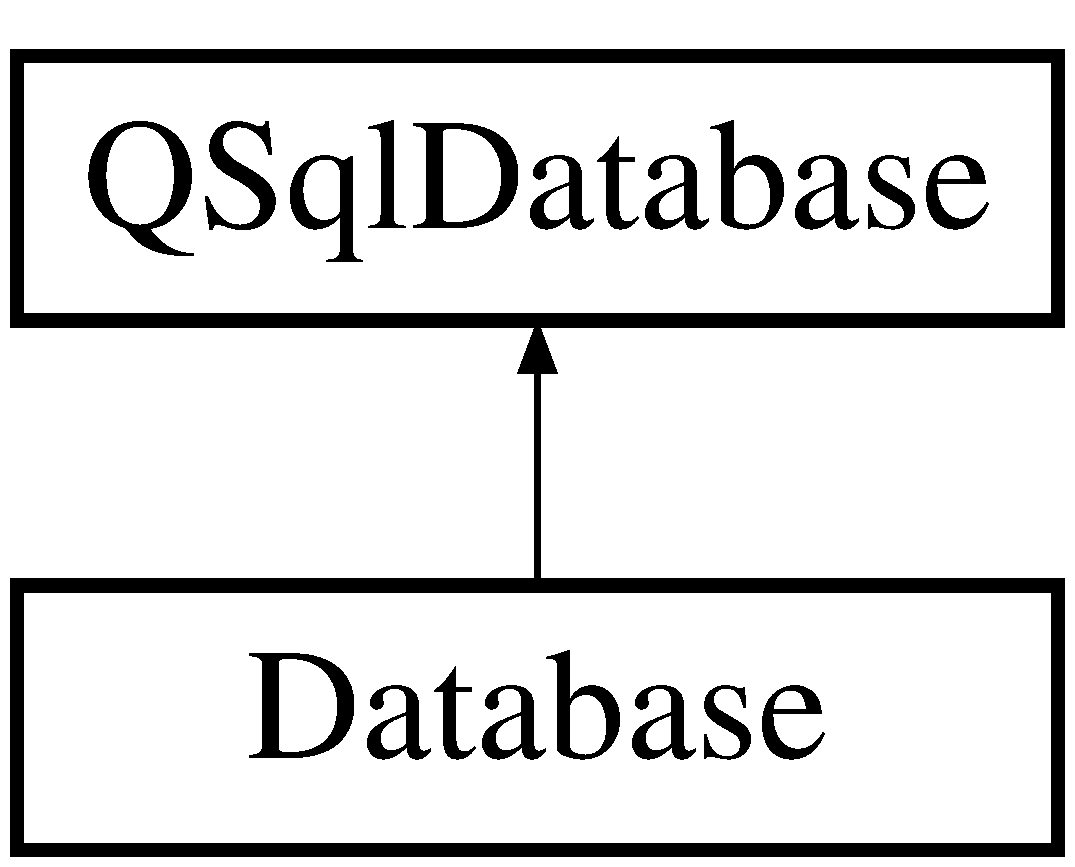
\includegraphics[height=2.000000cm]{class_database}
\end{center}
\end{figure}
\subsection*{Public Member Functions}
\begin{DoxyCompactItemize}
\item 
\hyperlink{class_database_a39f80fe1b43e44d840487fbe80034ff5}{Database} (Q\+String path, Q\+String driver)
\begin{DoxyCompactList}\small\item\em Create database from specified db file and driver. \end{DoxyCompactList}\item 
bool \hyperlink{class_database_a427744572ef7ae7489cb98d0638d3147}{Add\+Souvenir} (Q\+String stadium\+Name, Q\+String item\+Name, double item\+Price)
\begin{DoxyCompactList}\small\item\em Add a souvenir to a stadium\textquotesingle{}s souvenir list. \end{DoxyCompactList}\item 
bool \hyperlink{class_database_a6ce5328c14654001dc00760e8aa051dd}{Add\+Stadium} (Q\+String stadium\+Name, Q\+String team\+Name, Q\+String address, Q\+String phone\+Number, Q\+String date\+Opened, Q\+String capacity, Q\+String turf\+Type, long revenue, Q\+String leauge, Q\+String typology)
\begin{DoxyCompactList}\small\item\em Add a Stadium to Stadium\textquotesingle{}s data base. \end{DoxyCompactList}\item 
bool \hyperlink{class_database_a9b9d910bc03a31b4ba8a0247f4d87e35}{Add\+Distance} (int a, int b, long distance)
\begin{DoxyCompactList}\small\item\em Add edges between vertecies to distances database. \end{DoxyCompactList}\item 
bool \hyperlink{class_database_a7af2402bcaac82c92eb9954dc7435d32}{Add\+Revenue} (int id, double revenue)
\begin{DoxyCompactList}\small\item\em Alter a current stadium\textquotesingle{}s total revenue. \end{DoxyCompactList}\item 
Q\+String\+List \hyperlink{class_database_ae4ea1141f1aa1651da8854c4f16a5f00}{Get\+Stadium\+Names} ()
\begin{DoxyCompactList}\small\item\em Retrieve a list of stadium names. \end{DoxyCompactList}\item 
int \hyperlink{class_database_af3530b05506d54e45bd8fbdbcb72495d}{Get\+Stadium\+ID} (Q\+String name)
\begin{DoxyCompactList}\small\item\em Retrieve a stadium ID given the name. \end{DoxyCompactList}\item 
double \hyperlink{class_database_ac4b525f1a61d1b4fd11c81bd3b2c92b0}{Get\+Total\+Revenues} ()
\begin{DoxyCompactList}\small\item\em Retrieve the total amount of revenue from all stadiums. \end{DoxyCompactList}\item 
\hyperlink{class_database_a84d399a2ad58d69daab9b05330e1316d}{$\sim$\+Database} ()
\begin{DoxyCompactList}\small\item\em Destructor. \end{DoxyCompactList}\item 
Q\+Sql\+Query \hyperlink{class_database_a7a273ea995fbd9063ce67e46dbbadd27}{get\+Edges} ()
\begin{DoxyCompactList}\small\item\em Retrieve I\+Ds and Distances. \end{DoxyCompactList}\item 
int \hyperlink{class_database_a6d214ff690fe02bfade1943240c2bd27}{get\+Number\+Of\+Stadiums} () const 
\begin{DoxyCompactList}\small\item\em Return the number of stadiums in the database. \end{DoxyCompactList}\item 
Q\+Sql\+Query \hyperlink{class_database_a26fee1a206ddc5b9ed89242cfba29f92}{get\+Stadiums\+Name\+Id} ()
\begin{DoxyCompactList}\small\item\em Get the query containing the ids and stadium names available in the database. \end{DoxyCompactList}\item 
double \hyperlink{class_database_ac303418b93547f5106af47c542c7623b}{Get\+Revenue} (int id)
\begin{DoxyCompactList}\small\item\em Gets the revenue of the particular stadium given its ID. \end{DoxyCompactList}\item 
double \hyperlink{class_database_abff0f7f77d9a3a3b2ea62930c5935cf9}{Get\+Revenue} (Q\+String stadium\+Name)
\begin{DoxyCompactList}\small\item\em Gets the revenue of the particular stadium given its name. \end{DoxyCompactList}\end{DoxyCompactItemize}


\subsection{Detailed Description}
The \hyperlink{class_database}{Database} class is a wrapper for Q\+Sql\+Database. 

Definition at line 13 of file database.\+h.



\subsection{Constructor \& Destructor Documentation}
\index{Database@{Database}!Database@{Database}}
\index{Database@{Database}!Database@{Database}}
\subsubsection[{\texorpdfstring{Database(\+Q\+String path, Q\+String driver)}{Database(QString path, QString driver)}}]{\setlength{\rightskip}{0pt plus 5cm}Database\+::\+Database (
\begin{DoxyParamCaption}
\item[{Q\+String}]{path, }
\item[{Q\+String}]{driver}
\end{DoxyParamCaption}
)}\hypertarget{class_database_a39f80fe1b43e44d840487fbe80034ff5}{}\label{class_database_a39f80fe1b43e44d840487fbe80034ff5}


Create database from specified db file and driver. 

\hyperlink{class_database_a39f80fe1b43e44d840487fbe80034ff5}{Database\+::\+Database}.


\begin{DoxyParams}{Parameters}
{\em path} & Path to S\+QL \hyperlink{class_database}{Database} file \\
\hline
{\em driver} & Q\+String identifier for the specific flavor of S\+QL we are using. \\
\hline
\end{DoxyParams}


Definition at line 8 of file database.\+cpp.

\index{Database@{Database}!````~Database@{$\sim$\+Database}}
\index{````~Database@{$\sim$\+Database}!Database@{Database}}
\subsubsection[{\texorpdfstring{$\sim$\+Database()}{~Database()}}]{\setlength{\rightskip}{0pt plus 5cm}Database\+::$\sim$\+Database (
\begin{DoxyParamCaption}
{}
\end{DoxyParamCaption}
)}\hypertarget{class_database_a84d399a2ad58d69daab9b05330e1316d}{}\label{class_database_a84d399a2ad58d69daab9b05330e1316d}


Destructor. 



\subsection{Member Function Documentation}
\index{Database@{Database}!Add\+Distance@{Add\+Distance}}
\index{Add\+Distance@{Add\+Distance}!Database@{Database}}
\subsubsection[{\texorpdfstring{Add\+Distance(int a, int b, long distance)}{AddDistance(int a, int b, long distance)}}]{\setlength{\rightskip}{0pt plus 5cm}bool Database\+::\+Add\+Distance (
\begin{DoxyParamCaption}
\item[{int}]{a, }
\item[{int}]{b, }
\item[{long}]{distance}
\end{DoxyParamCaption}
)}\hypertarget{class_database_a9b9d910bc03a31b4ba8a0247f4d87e35}{}\label{class_database_a9b9d910bc03a31b4ba8a0247f4d87e35}


Add edges between vertecies to distances database. 

\hyperlink{class_database_a9b9d910bc03a31b4ba8a0247f4d87e35}{Database\+::\+Add\+Distance} Adds new distacne between two vertecies.


\begin{DoxyParams}{Parameters}
{\em a} & starting vertex \\
\hline
{\em b} & ending vertex \\
\hline
{\em distance} & weight of the edge \\
\hline
\end{DoxyParams}
\begin{DoxyReturn}{Returns}
true if it worked else false 
\end{DoxyReturn}


Definition at line 173 of file database.\+cpp.

\index{Database@{Database}!Add\+Revenue@{Add\+Revenue}}
\index{Add\+Revenue@{Add\+Revenue}!Database@{Database}}
\subsubsection[{\texorpdfstring{Add\+Revenue(int id, double revenue)}{AddRevenue(int id, double revenue)}}]{\setlength{\rightskip}{0pt plus 5cm}bool Database\+::\+Add\+Revenue (
\begin{DoxyParamCaption}
\item[{int}]{id, }
\item[{double}]{revenue}
\end{DoxyParamCaption}
)}\hypertarget{class_database_a7af2402bcaac82c92eb9954dc7435d32}{}\label{class_database_a7af2402bcaac82c92eb9954dc7435d32}


Alter a current stadium\textquotesingle{}s total revenue. 

\hyperlink{class_database_a7af2402bcaac82c92eb9954dc7435d32}{Database\+::\+Add\+Revenue} Add amount to revenue attribute in stadiums table.


\begin{DoxyParams}{Parameters}
{\em id} & stadiums id \\
\hline
{\em revenue} & of the stadium \\
\hline
\end{DoxyParams}
\begin{DoxyReturn}{Returns}

\end{DoxyReturn}


Definition at line 195 of file database.\+cpp.

\index{Database@{Database}!Add\+Souvenir@{Add\+Souvenir}}
\index{Add\+Souvenir@{Add\+Souvenir}!Database@{Database}}
\subsubsection[{\texorpdfstring{Add\+Souvenir(\+Q\+String stadium\+Name, Q\+String item\+Name, double item\+Price)}{AddSouvenir(QString stadiumName, QString itemName, double itemPrice)}}]{\setlength{\rightskip}{0pt plus 5cm}bool Database\+::\+Add\+Souvenir (
\begin{DoxyParamCaption}
\item[{Q\+String}]{stadium\+Name, }
\item[{Q\+String}]{item\+Name, }
\item[{double}]{item\+Price}
\end{DoxyParamCaption}
)}\hypertarget{class_database_a427744572ef7ae7489cb98d0638d3147}{}\label{class_database_a427744572ef7ae7489cb98d0638d3147}


Add a souvenir to a stadium\textquotesingle{}s souvenir list. 

\hyperlink{class_database_a427744572ef7ae7489cb98d0638d3147}{Database\+::\+Add\+Souvenir} Add a souvenir to a certain stadium\textquotesingle{}s souvenir list given the stadium\textquotesingle{}s name.


\begin{DoxyParams}{Parameters}
{\em stadium\+Name} & The stadium name \\
\hline
{\em item\+Name} & The item name \\
\hline
{\em item\+Price} & The item price \\
\hline
\end{DoxyParams}
\begin{DoxyReturn}{Returns}
true if it worked 
\end{DoxyReturn}


Definition at line 101 of file database.\+cpp.

\index{Database@{Database}!Add\+Stadium@{Add\+Stadium}}
\index{Add\+Stadium@{Add\+Stadium}!Database@{Database}}
\subsubsection[{\texorpdfstring{Add\+Stadium(\+Q\+String stadium\+Name, Q\+String team\+Name, Q\+String address, Q\+String phone\+Number, Q\+String date\+Opened, Q\+String capacity, Q\+String turf\+Type, long revenue, Q\+String leauge, Q\+String typology)}{AddStadium(QString stadiumName, QString teamName, QString address, QString phoneNumber, QString dateOpened, QString capacity, QString turfType, long revenue, QString leauge, QString typology)}}]{\setlength{\rightskip}{0pt plus 5cm}bool Database\+::\+Add\+Stadium (
\begin{DoxyParamCaption}
\item[{Q\+String}]{stadium\+Name, }
\item[{Q\+String}]{team\+Name, }
\item[{Q\+String}]{address, }
\item[{Q\+String}]{phone\+Number, }
\item[{Q\+String}]{date\+Opened, }
\item[{Q\+String}]{capacity, }
\item[{Q\+String}]{turf\+Type, }
\item[{long}]{revenue, }
\item[{Q\+String}]{leauge, }
\item[{Q\+String}]{typology}
\end{DoxyParamCaption}
)}\hypertarget{class_database_a6ce5328c14654001dc00760e8aa051dd}{}\label{class_database_a6ce5328c14654001dc00760e8aa051dd}


Add a Stadium to Stadium\textquotesingle{}s data base. 

\hyperlink{class_database_a6ce5328c14654001dc00760e8aa051dd}{Database\+::\+Add\+Stadium} Adds new Stadium to the data base with the following attributes.


\begin{DoxyParams}{Parameters}
{\em stadium\+Name} & \\
\hline
{\em team\+Name} & \\
\hline
{\em address} & \\
\hline
{\em phone\+Number} & \\
\hline
{\em date\+Opened} & \\
\hline
{\em capacity} & \\
\hline
{\em turf\+Type} & \\
\hline
{\em revenue} & \\
\hline
{\em leauge} & \\
\hline
{\em typology} & \\
\hline
\end{DoxyParams}
\begin{DoxyReturn}{Returns}
true if it worked else false 
\end{DoxyReturn}


Definition at line 140 of file database.\+cpp.

\index{Database@{Database}!get\+Edges@{get\+Edges}}
\index{get\+Edges@{get\+Edges}!Database@{Database}}
\subsubsection[{\texorpdfstring{get\+Edges()}{getEdges()}}]{\setlength{\rightskip}{0pt plus 5cm}Q\+Sql\+Query Database\+::get\+Edges (
\begin{DoxyParamCaption}
{}
\end{DoxyParamCaption}
)}\hypertarget{class_database_a7a273ea995fbd9063ce67e46dbbadd27}{}\label{class_database_a7a273ea995fbd9063ce67e46dbbadd27}


Retrieve I\+Ds and Distances. 

\hyperlink{class_database_a7a273ea995fbd9063ce67e46dbbadd27}{Database\+::get\+Edges} Method that executes a S\+QL query to grab all ids to, ids from and distances from the distances table.

\begin{DoxyReturn}{Returns}
S\+Q\+Lquery containing the results of the 
\end{DoxyReturn}


Definition at line 35 of file database.\+cpp.

\index{Database@{Database}!get\+Number\+Of\+Stadiums@{get\+Number\+Of\+Stadiums}}
\index{get\+Number\+Of\+Stadiums@{get\+Number\+Of\+Stadiums}!Database@{Database}}
\subsubsection[{\texorpdfstring{get\+Number\+Of\+Stadiums() const }{getNumberOfStadiums() const }}]{\setlength{\rightskip}{0pt plus 5cm}int Database\+::get\+Number\+Of\+Stadiums (
\begin{DoxyParamCaption}
{}
\end{DoxyParamCaption}
) const}\hypertarget{class_database_a6d214ff690fe02bfade1943240c2bd27}{}\label{class_database_a6d214ff690fe02bfade1943240c2bd27}


Return the number of stadiums in the database. 

\hyperlink{class_database_a6d214ff690fe02bfade1943240c2bd27}{Database\+::get\+Number\+Of\+Stadiums} Method executes a sql query to get the total number of stadiums in the database.

\begin{DoxyReturn}{Returns}
int value \# of stadiums 
\end{DoxyReturn}


Definition at line 58 of file database.\+cpp.

\index{Database@{Database}!Get\+Revenue@{Get\+Revenue}}
\index{Get\+Revenue@{Get\+Revenue}!Database@{Database}}
\subsubsection[{\texorpdfstring{Get\+Revenue(int id)}{GetRevenue(int id)}}]{\setlength{\rightskip}{0pt plus 5cm}double Database\+::\+Get\+Revenue (
\begin{DoxyParamCaption}
\item[{int}]{id}
\end{DoxyParamCaption}
)}\hypertarget{class_database_ac303418b93547f5106af47c542c7623b}{}\label{class_database_ac303418b93547f5106af47c542c7623b}


Gets the revenue of the particular stadium given its ID. 

Get\+Revenue Retrieve the current revenue value of a stadium given its ID.


\begin{DoxyParams}{Parameters}
{\em id} & stadium ID \\
\hline
\end{DoxyParams}
\begin{DoxyReturn}{Returns}
the current revenue of the stadium 
\end{DoxyReturn}


Definition at line 305 of file database.\+cpp.

\index{Database@{Database}!Get\+Revenue@{Get\+Revenue}}
\index{Get\+Revenue@{Get\+Revenue}!Database@{Database}}
\subsubsection[{\texorpdfstring{Get\+Revenue(\+Q\+String stadium\+Name)}{GetRevenue(QString stadiumName)}}]{\setlength{\rightskip}{0pt plus 5cm}double Database\+::\+Get\+Revenue (
\begin{DoxyParamCaption}
\item[{Q\+String}]{stadium\+Name}
\end{DoxyParamCaption}
)}\hypertarget{class_database_abff0f7f77d9a3a3b2ea62930c5935cf9}{}\label{class_database_abff0f7f77d9a3a3b2ea62930c5935cf9}


Gets the revenue of the particular stadium given its name. 

Get\+Revenue Retrieve the current revenue value of a stadium given its name.


\begin{DoxyParams}{Parameters}
{\em id} & stadium ID \\
\hline
\end{DoxyParams}
\begin{DoxyReturn}{Returns}
the current revenue of the stadium 
\end{DoxyReturn}


Definition at line 333 of file database.\+cpp.

\index{Database@{Database}!Get\+Stadium\+ID@{Get\+Stadium\+ID}}
\index{Get\+Stadium\+ID@{Get\+Stadium\+ID}!Database@{Database}}
\subsubsection[{\texorpdfstring{Get\+Stadium\+I\+D(\+Q\+String name)}{GetStadiumID(QString name)}}]{\setlength{\rightskip}{0pt plus 5cm}int Database\+::\+Get\+Stadium\+ID (
\begin{DoxyParamCaption}
\item[{Q\+String}]{name}
\end{DoxyParamCaption}
)}\hypertarget{class_database_af3530b05506d54e45bd8fbdbcb72495d}{}\label{class_database_af3530b05506d54e45bd8fbdbcb72495d}


Retrieve a stadium ID given the name. 

\hyperlink{class_database_af3530b05506d54e45bd8fbdbcb72495d}{Database\+::\+Get\+Stadium\+ID} Retrieve a stadium\textquotesingle{}s unique ID given its name.


\begin{DoxyParams}{Parameters}
{\em name} & the stadium name \\
\hline
\end{DoxyParams}
\begin{DoxyReturn}{Returns}
the stadium ID 
\end{DoxyReturn}


Definition at line 250 of file database.\+cpp.

\index{Database@{Database}!Get\+Stadium\+Names@{Get\+Stadium\+Names}}
\index{Get\+Stadium\+Names@{Get\+Stadium\+Names}!Database@{Database}}
\subsubsection[{\texorpdfstring{Get\+Stadium\+Names()}{GetStadiumNames()}}]{\setlength{\rightskip}{0pt plus 5cm}Q\+String\+List Database\+::\+Get\+Stadium\+Names (
\begin{DoxyParamCaption}
{}
\end{DoxyParamCaption}
)}\hypertarget{class_database_ae4ea1141f1aa1651da8854c4f16a5f00}{}\label{class_database_ae4ea1141f1aa1651da8854c4f16a5f00}


Retrieve a list of stadium names. 

\hyperlink{class_database_ae4ea1141f1aa1651da8854c4f16a5f00}{Database\+::\+Get\+Stadium\+Names} Retrieve a list of stadium names.

\begin{DoxyReturn}{Returns}
names a list of stadium names 
\end{DoxyReturn}


Definition at line 228 of file database.\+cpp.

\index{Database@{Database}!get\+Stadiums\+Name\+Id@{get\+Stadiums\+Name\+Id}}
\index{get\+Stadiums\+Name\+Id@{get\+Stadiums\+Name\+Id}!Database@{Database}}
\subsubsection[{\texorpdfstring{get\+Stadiums\+Name\+Id()}{getStadiumsNameId()}}]{\setlength{\rightskip}{0pt plus 5cm}Q\+Sql\+Query Database\+::get\+Stadiums\+Name\+Id (
\begin{DoxyParamCaption}
{}
\end{DoxyParamCaption}
)}\hypertarget{class_database_a26fee1a206ddc5b9ed89242cfba29f92}{}\label{class_database_a26fee1a206ddc5b9ed89242cfba29f92}


Get the query containing the ids and stadium names available in the database. 

\hyperlink{class_database_a26fee1a206ddc5b9ed89242cfba29f92}{Database\+::get\+Stadiums\+Name\+Id} Get the name, and ID of each of the stadiums from the database and order the results by id, descending order.

\begin{DoxyReturn}{Returns}
S\+Q\+L\+Query containing the results from the exeuction 
\end{DoxyReturn}


Definition at line 76 of file database.\+cpp.

\index{Database@{Database}!Get\+Total\+Revenues@{Get\+Total\+Revenues}}
\index{Get\+Total\+Revenues@{Get\+Total\+Revenues}!Database@{Database}}
\subsubsection[{\texorpdfstring{Get\+Total\+Revenues()}{GetTotalRevenues()}}]{\setlength{\rightskip}{0pt plus 5cm}double Database\+::\+Get\+Total\+Revenues (
\begin{DoxyParamCaption}
{}
\end{DoxyParamCaption}
)}\hypertarget{class_database_ac4b525f1a61d1b4fd11c81bd3b2c92b0}{}\label{class_database_ac4b525f1a61d1b4fd11c81bd3b2c92b0}


Retrieve the total amount of revenue from all stadiums. 

\hyperlink{class_database_ac4b525f1a61d1b4fd11c81bd3b2c92b0}{Database\+::\+Get\+Total\+Revenues}.

\begin{DoxyReturn}{Returns}
The sum of all stadium revenues 
\end{DoxyReturn}


Definition at line 273 of file database.\+cpp.



The documentation for this class was generated from the following files\+:\begin{DoxyCompactItemize}
\item 
src/header/\hyperlink{database_8h}{database.\+h}\item 
src/source/\hyperlink{database_8cpp}{database.\+cpp}\end{DoxyCompactItemize}

\hypertarget{struct_edge}{}\section{Edge Struct Reference}
\label{struct_edge}\index{Edge@{Edge}}


{\ttfamily \#include $<$vertex.\+h$>$}

\subsection*{Public Attributes}
\begin{DoxyCompactItemize}
\item 
int \hyperlink{struct_edge_ad1319391eee273abf83c98be4780d19e}{id\+From}
\item 
int \hyperlink{struct_edge_aabcf5e86aeb614464438885671124b0d}{id\+To}
\item 
int \hyperlink{struct_edge_a4d58e1f4de38fa55549497175981ebab}{weight}
\end{DoxyCompactItemize}


\subsection{Detailed Description}


Definition at line 9 of file vertex.\+h.



\subsection{Member Data Documentation}
\index{Edge@{Edge}!id\+From@{id\+From}}
\index{id\+From@{id\+From}!Edge@{Edge}}
\subsubsection[{\texorpdfstring{id\+From}{idFrom}}]{\setlength{\rightskip}{0pt plus 5cm}int Edge\+::id\+From}\hypertarget{struct_edge_ad1319391eee273abf83c98be4780d19e}{}\label{struct_edge_ad1319391eee273abf83c98be4780d19e}


Definition at line 11 of file vertex.\+h.

\index{Edge@{Edge}!id\+To@{id\+To}}
\index{id\+To@{id\+To}!Edge@{Edge}}
\subsubsection[{\texorpdfstring{id\+To}{idTo}}]{\setlength{\rightskip}{0pt plus 5cm}int Edge\+::id\+To}\hypertarget{struct_edge_aabcf5e86aeb614464438885671124b0d}{}\label{struct_edge_aabcf5e86aeb614464438885671124b0d}


Definition at line 12 of file vertex.\+h.

\index{Edge@{Edge}!weight@{weight}}
\index{weight@{weight}!Edge@{Edge}}
\subsubsection[{\texorpdfstring{weight}{weight}}]{\setlength{\rightskip}{0pt plus 5cm}int Edge\+::weight}\hypertarget{struct_edge_a4d58e1f4de38fa55549497175981ebab}{}\label{struct_edge_a4d58e1f4de38fa55549497175981ebab}


Definition at line 13 of file vertex.\+h.



The documentation for this struct was generated from the following file\+:\begin{DoxyCompactItemize}
\item 
src/header/\hyperlink{vertex_8h}{vertex.\+h}\end{DoxyCompactItemize}

\hypertarget{class_edit_stadium_info}{}\section{Edit\+Stadium\+Info Class Reference}
\label{class_edit_stadium_info}\index{Edit\+Stadium\+Info@{Edit\+Stadium\+Info}}


{\ttfamily \#include $<$editstadiuminfo.\+h$>$}

Inheritance diagram for Edit\+Stadium\+Info\+:\begin{figure}[H]
\begin{center}
\leavevmode
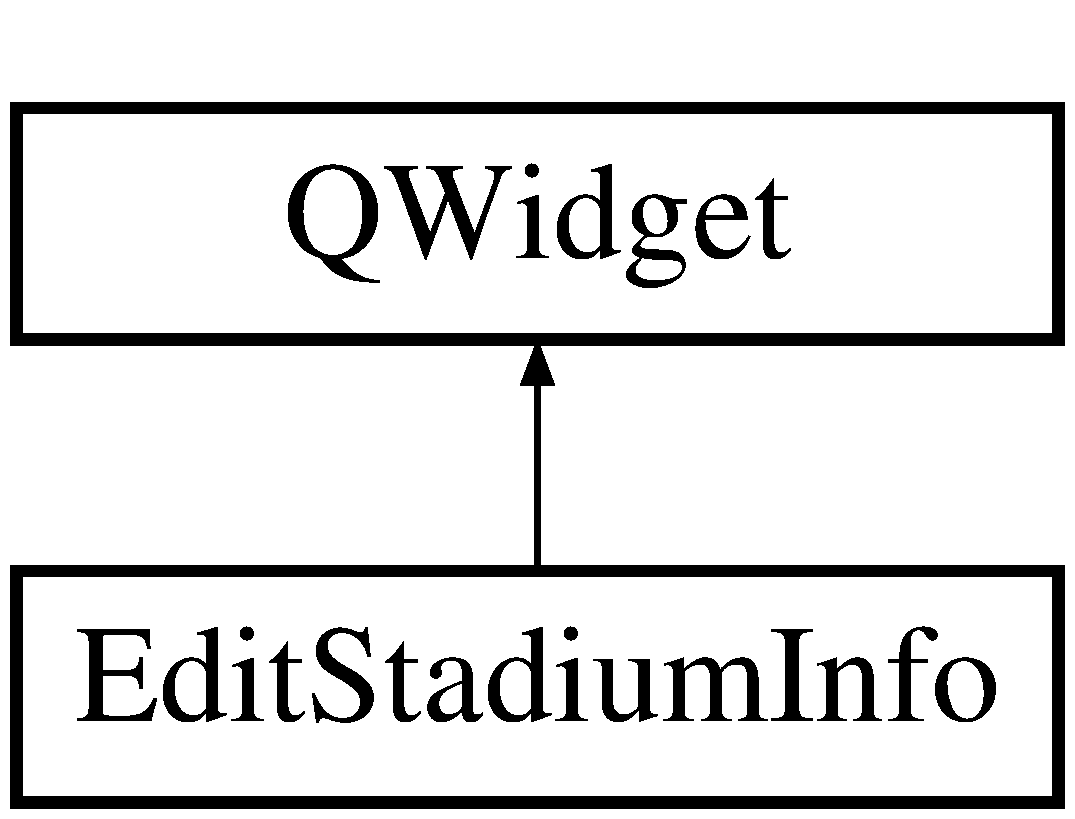
\includegraphics[height=2.000000cm]{class_edit_stadium_info}
\end{center}
\end{figure}
\subsection*{Public Member Functions}
\begin{DoxyCompactItemize}
\item 
\hyperlink{class_edit_stadium_info_a483072706867eccd6d0c20888da7f71c}{Edit\+Stadium\+Info} (Q\+Widget $\ast$parent=0)
\item 
\hyperlink{class_edit_stadium_info_a765634ed0735c47695013c5b66083458}{$\sim$\+Edit\+Stadium\+Info} ()
\end{DoxyCompactItemize}


\subsection{Detailed Description}


Definition at line 10 of file editstadiuminfo.\+h.



\subsection{Constructor \& Destructor Documentation}
\index{Edit\+Stadium\+Info@{Edit\+Stadium\+Info}!Edit\+Stadium\+Info@{Edit\+Stadium\+Info}}
\index{Edit\+Stadium\+Info@{Edit\+Stadium\+Info}!Edit\+Stadium\+Info@{Edit\+Stadium\+Info}}
\subsubsection[{\texorpdfstring{Edit\+Stadium\+Info(\+Q\+Widget $\ast$parent=0)}{EditStadiumInfo(QWidget *parent=0)}}]{\setlength{\rightskip}{0pt plus 5cm}Edit\+Stadium\+Info\+::\+Edit\+Stadium\+Info (
\begin{DoxyParamCaption}
\item[{Q\+Widget $\ast$}]{parent = {\ttfamily 0}}
\end{DoxyParamCaption}
)\hspace{0.3cm}{\ttfamily [explicit]}}\hypertarget{class_edit_stadium_info_a483072706867eccd6d0c20888da7f71c}{}\label{class_edit_stadium_info_a483072706867eccd6d0c20888da7f71c}


Definition at line 4 of file editstadiuminfo.\+cpp.

\index{Edit\+Stadium\+Info@{Edit\+Stadium\+Info}!````~Edit\+Stadium\+Info@{$\sim$\+Edit\+Stadium\+Info}}
\index{````~Edit\+Stadium\+Info@{$\sim$\+Edit\+Stadium\+Info}!Edit\+Stadium\+Info@{Edit\+Stadium\+Info}}
\subsubsection[{\texorpdfstring{$\sim$\+Edit\+Stadium\+Info()}{~EditStadiumInfo()}}]{\setlength{\rightskip}{0pt plus 5cm}Edit\+Stadium\+Info\+::$\sim$\+Edit\+Stadium\+Info (
\begin{DoxyParamCaption}
{}
\end{DoxyParamCaption}
)}\hypertarget{class_edit_stadium_info_a765634ed0735c47695013c5b66083458}{}\label{class_edit_stadium_info_a765634ed0735c47695013c5b66083458}


Definition at line 11 of file editstadiuminfo.\+cpp.



The documentation for this class was generated from the following files\+:\begin{DoxyCompactItemize}
\item 
src/header/\hyperlink{editstadiuminfo_8h}{editstadiuminfo.\+h}\item 
src/source/\hyperlink{editstadiuminfo_8cpp}{editstadiuminfo.\+cpp}\end{DoxyCompactItemize}

\hypertarget{class_example_class}{}\section{Example\+Class Class Reference}
\label{class_example_class}\index{Example\+Class@{Example\+Class}}


Provide an example $\ast$.  




\subsection{Detailed Description}
Provide an example $\ast$. 


\begin{DoxyItemize}
\item 
\item $\ast$ This class is meant as an example. It is not useful by itself
\item rather its usefulness is only a function of how much it helps
\item the reader. It is in a sense defined by the person who reads it
\item and otherwise does not exist in any real form.
\item 
\item \begin{DoxyNote}{Note}
Attempts at zen rarely work.
\end{DoxyNote}

\item 
\item \begin{DoxyAuthor}{Author}
(last to touch it) 
\end{DoxyAuthor}
\begin{DoxyParagraph}{Author}
bv 
\end{DoxyParagraph}

\item 
\item \begin{DoxyVersion}{Version}

\end{DoxyVersion}
\begin{DoxyParagraph}{Revision}
1.\+5 
\end{DoxyParagraph}

\item 
\item \begin{DoxyDate}{Date}

\end{DoxyDate}
\begin{DoxyParagraph}{Date}
2005/04/14 14\+:16\+:20 
\end{DoxyParagraph}

\item 
\item Contact\+: \href{mailto:bv@bnl.gov}{\tt bv@bnl.\+gov}
\item 
\item Created on\+: Wed Apr 13 18\+:39\+:37 2005
\item 
\item \begin{DoxyParagraph}{Id}
doxygen-\/howto.\+html,v 1.\+5 2005/04/14 14\+:16\+:20 bv Exp 
\end{DoxyParagraph}

\item $\ast$/
\end{DoxyItemize}

\#ifndef E\+X\+A\+M\+P\+L\+E\+C\+L\+A\+S\+S\+\_\+H \#define E\+X\+A\+M\+P\+L\+E\+C\+L\+A\+S\+S\+\_\+H

class \hyperlink{class_example_class}{Example\+Class} \{

public\+: \begin{DoxyVerb}/// Create an ExampleClass
ExampleClass();

/// Create an ExampleClass with lot's of intial values
ExampleClass(int a, float b);

~ExampleClass();

/// This method does something
void DoSomething();

/** This is a method that does so
  * much that I must write an epic 
  * novel just to describe how much
  * it truly does. */
void DoNothing();

/**A useful method.
  * \param level an integer setting how useful to be
  * \return Output that is extra useful
  * 
  * This method does unbelievably useful things.  
  * And returns exceptionally useful results.
  * Use it everyday with good health.
  */
void* VeryUsefulMethod(bool level);
\end{DoxyVerb}


private\+: \begin{DoxyVerb}const char* fQuestion; ///< the question
int fAnswer;           ///< the answer 
\end{DoxyVerb}


\}; // end of class \hyperlink{class_example_class}{Example\+Class}

\#endif // E\+X\+A\+M\+P\+L\+E\+C\+L\+A\+S\+S\+\_\+H ```

\paragraph*{Unit Tests}


\begin{DoxyItemize}
\item All team members are responsible for writing unit tests for their own code.
\item Simply add the unit test to its appropriate section in \hyperlink{test__main_8cpp}{test\+\_\+main.\+cpp}. Note\+: This currently isn\textquotesingle{}t working properly. Still you should try to add unit tests as you code.
\end{DoxyItemize}

\paragraph*{General Style Guide}


\begin{DoxyItemize}
\item For this project we will be following, loosely, \href{https://google.github.io/styleguide/cppguide.html}{\tt Google\textquotesingle{}s C++ Style Guide}. Have a quick read through of some of the sections. This is where we will refer to if there are disagreements about style. 
\end{DoxyItemize}

The documentation for this class was generated from the following file\+:\begin{DoxyCompactItemize}
\item 
\hyperlink{_r_e_a_d_m_e_8md}{R\+E\+A\+D\+M\+E.\+md}\end{DoxyCompactItemize}

\hypertarget{class_graph}{}\section{Graph Class Reference}
\label{class_graph}\index{Graph@{Graph}}


{\ttfamily \#include $<$graph.\+h$>$}

\subsection*{Public Member Functions}
\begin{DoxyCompactItemize}
\item 
\hyperlink{class_graph_ae4c72b8ac4d693c49800a4c7e273654f}{Graph} ()
\item 
\hyperlink{class_graph_a902c5b3eacb66d60752525ab23297a95}{$\sim$\+Graph} ()
\begin{DoxyCompactList}\small\item\em Deconstructor, deallocates the memory set by the Adjacency Matrix. \end{DoxyCompactList}\item 
int \hyperlink{class_graph_ae4cc9fd62a6dbe9e42ee0de8128b8b86}{edge\+Weight} (int v1, int v2)
\begin{DoxyCompactList}\small\item\em edge\+Weight Method provides a safe way to access the adjacency matrix. \end{DoxyCompactList}\item 
\hyperlink{class_q_list}{Q\+List}$<$ \hyperlink{class_vertex}{Vertex} $>$ \hyperlink{class_graph_aacba6816dff17b52d3636f3448953ed3}{get\+Vertices} () const 
\begin{DoxyCompactList}\small\item\em get\+Vertex\+List This will return a \hyperlink{class_q_list}{Q\+List} of vertices in the graph. \end{DoxyCompactList}\item 
void \hyperlink{class_graph_aac58209df6c10a710770a641b86faf79}{create\+Graph} (\hyperlink{class_database}{Database} $\ast$db)
\begin{DoxyCompactList}\small\item\em create\+Graph This method will call in the database and generate the graph that includes edges, and vertices. These represent the stadiums and the paths a baseball fan is able to \end{DoxyCompactList}\item 
void \hyperlink{class_graph_a3eb1eaf4a580710194c014d0e135c7b6}{shortest\+Path} (\hyperlink{class_vertex}{Vertex} source)
\begin{DoxyCompactList}\small\item\em shortest\+Path Returns the shortest path given the starting ID of a vertex. \end{DoxyCompactList}\item 
void \hyperlink{class_graph_a6fc020710dd252058c006961f33f2b4b}{shortest\+Path} (int source)
\begin{DoxyCompactList}\small\item\em shortest\+Path Returns the shortest path given the starting ID of a vertex. \end{DoxyCompactList}\item 
void \hyperlink{class_graph_ad1c7af5ab7a9fc6ce190779170bb655c}{clear\+Graph} ()
\begin{DoxyCompactList}\small\item\em clear\+Graph This method clears the current graph T\+O\+DO\+: Needs to be updated for the current implementation of the graph search. \end{DoxyCompactList}\item 
int \hyperlink{class_graph_ae60b31b9a4779dee8145b4e66798dfbe}{get\+Number\+Vertices} () const 
\begin{DoxyCompactList}\small\item\em get\+Number\+Vertices This method returns the number of vertices that are inserted in the graph \end{DoxyCompactList}\item 
long \hyperlink{class_graph_ac855f8082b6b9931c065541c56086124}{get\+Total\+Distance} () const 
\begin{DoxyCompactList}\small\item\em get\+Total\+Distance Calculates the total distance going to all vertices starting at dodger stadium each time. \end{DoxyCompactList}\item 
\hyperlink{class_q_list}{Q\+List}$<$ \hyperlink{class_vertex}{Vertex} $>$ \hyperlink{class_graph_a09a9556b35c23b793429ba9433543a74}{get\+Vertex\+Path} (\hyperlink{class_vertex}{Vertex} target)
\begin{DoxyCompactList}\small\item\em \hyperlink{class_graph_a09a9556b35c23b793429ba9433543a74}{Graph\+::get\+Vertex\+Path} Function will take a given vertex and traverse up the path of the given parent ids to construct the path that was taken to arrive at the target vertex. This method will return a \hyperlink{class_q_list}{Q\+List} of vertices, where index 0 is the starting vertice and the last vertex in the list is the given target vertex. \end{DoxyCompactList}\item 
\hyperlink{class_q_list}{Q\+List}$<$ \hyperlink{class_vertex}{Vertex} $>$ \hyperlink{class_graph_a0236e44d9f8e625d7dd370977e279e4d}{get\+Vertex\+Path} (int target)
\begin{DoxyCompactList}\small\item\em \hyperlink{class_graph_a09a9556b35c23b793429ba9433543a74}{Graph\+::get\+Vertex\+Path} Function will take a given vertex and traverse up the path of the given parent ids to construct the path that was taken to arrive at the target vertex. This method will return a \hyperlink{class_q_list}{Q\+List} of vertices, where index 0 is the starting vertice and the last vertex in the list is the given target vertex. \end{DoxyCompactList}\item 
\hyperlink{class_q_list}{Q\+List}$<$ \hyperlink{class_vertex}{Vertex} $>$ \hyperlink{class_graph_aa752bbc142469ed2f79c15121bfb61c7}{find\+Shortest\+Path\+To} (\hyperlink{class_database}{Database} $\ast$db, int source, int target)
\begin{DoxyCompactList}\small\item\em \hyperlink{class_graph_aa752bbc142469ed2f79c15121bfb61c7}{Graph\+::find\+Shortest\+Path\+To} This is an overloaded method for find the shortest path between 2 vertices. It calls on other methods such as creating the graph, finding the shortest path to all vertices then getting the target vertex from the vertex list. After the algorithm has found the shortest path, it will return a \hyperlink{class_q_list}{Q\+List} of vertices in which it is required to traverse to get to the target vertex. The list will contain the starting vertex and ending vertex. Each vertex will have a distance value it takes to get to that vertex given the starting the vertex. \end{DoxyCompactList}\item 
\hyperlink{class_q_list}{Q\+List}$<$ \hyperlink{class_vertex}{Vertex} $>$ \hyperlink{class_graph_a3f648a5d4a3ebd43dfde49545ea76d07}{find\+Shortest\+Path\+To} (\hyperlink{class_database}{Database} $\ast$db, int source, \hyperlink{class_q_list}{Q\+List}$<$ int $>$ stops)
\begin{DoxyCompactList}\small\item\em \hyperlink{class_graph_aa752bbc142469ed2f79c15121bfb61c7}{Graph\+::find\+Shortest\+Path\+To} This is an overloaded method for find the shortest path between a starting vertex, and a list of vertices. It calls on other methods such as creating the graph, finding the shortest path to all vertices then getting the target vertex from the vertex list. After the algorithm has found the shortest path, it will return a \hyperlink{class_q_list}{Q\+List} of vertices in which it is required to traverse to get to the target vertex. The list will contain the starting vertex and ending vertex. Each vertex will have a distance value it takes to get to that vertex given the starting the vertex. \end{DoxyCompactList}\item 
long \hyperlink{class_graph_ab3c693e0fce0a24e32893b750b0ca82f}{minimum\+Spanning\+Tree} (int source)
\begin{DoxyCompactList}\small\item\em minimum\+Spanning\+Tree This method will generate the minimum spanning tree given a starting vertex. It is recommended not to start at index 0, 1, 22, or 29 to guarantee the most minimum spanning tree possible in the given graph. Each vertex will store the parent of the vertex that it had to traverse to get to. \end{DoxyCompactList}\item 
\hyperlink{class_q_list}{Q\+List}$<$ \hyperlink{class_vertex}{Vertex} $>$ \hyperlink{class_graph_a2a404d20921b9f68e9d31baeb7079293}{get\+Dodger\+Stadium\+Path} ()
\begin{DoxyCompactList}\small\item\em get\+Dodger\+Stadium\+Path This is a specialized function for finding the shortest path using dijkstra\textquotesingle{}s algorithm starting at Dodger stadium. \end{DoxyCompactList}\item 
void \hyperlink{class_graph_a6bb74d3d522a6a788296839481278f48}{debug\+\_\+print\+Adj\+Matrix} () const 
\begin{DoxyCompactList}\small\item\em debug\+\_\+print\+Adj\+Matrix Method for debugging the adjacency matrix, will only output to the console, nothing else. \end{DoxyCompactList}\item 
void \hyperlink{class_graph_a7e75b59c73495734103b055e70a561bb}{debug\+\_\+output\+Distances} () const 
\begin{DoxyCompactList}\small\item\em debug\+\_\+output\+Distances Method for outputting all the distances found after performing dijkstra\textquotesingle{}s algorithm for finding the shortest path to all vertices. \end{DoxyCompactList}\item 
void \hyperlink{class_graph_abd2cdd5f963d7f820de8d2b0e6f37685}{debug\+\_\+print\+Path} (\hyperlink{class_vertex}{Vertex} vertex) const 
\begin{DoxyCompactList}\small\item\em \hyperlink{class_graph_abd2cdd5f963d7f820de8d2b0e6f37685}{Graph\+::debug\+\_\+print\+Path} Debugging method for printing the path found to the given vertex. This will only work after a search for the shortest path has been found. \end{DoxyCompactList}\item 
long \hyperlink{class_graph_a6ce87b850b22cc6deed2b58f3760c4a9}{min\+Key} (long key\mbox{[}$\,$\mbox{]}, bool mst\+Set\mbox{[}$\,$\mbox{]})
\begin{DoxyCompactList}\small\item\em \hyperlink{class_graph_a6ce87b850b22cc6deed2b58f3760c4a9}{Graph\+::min\+Key} Utility function to find the vertex with minimum key value, from the set of vertices not yet included in the minimum spanning tree. \end{DoxyCompactList}\item 
\hyperlink{class_q_list}{Q\+List}$<$ \hyperlink{class_vertex}{Vertex} $>$ \hyperlink{class_graph_ab9c6180a6194d2b0cb702a998fa74175}{mst} ()
\end{DoxyCompactItemize}


\subsection{Detailed Description}


Definition at line 14 of file graph.\+h.



\subsection{Constructor \& Destructor Documentation}
\index{Graph@{Graph}!Graph@{Graph}}
\index{Graph@{Graph}!Graph@{Graph}}
\subsubsection[{\texorpdfstring{Graph()}{Graph()}}]{\setlength{\rightskip}{0pt plus 5cm}Graph\+::\+Graph (
\begin{DoxyParamCaption}
{}
\end{DoxyParamCaption}
)}\hypertarget{class_graph_ae4c72b8ac4d693c49800a4c7e273654f}{}\label{class_graph_ae4c72b8ac4d693c49800a4c7e273654f}


Definition at line 7 of file graph.\+cpp.

\index{Graph@{Graph}!````~Graph@{$\sim$\+Graph}}
\index{````~Graph@{$\sim$\+Graph}!Graph@{Graph}}
\subsubsection[{\texorpdfstring{$\sim$\+Graph()}{~Graph()}}]{\setlength{\rightskip}{0pt plus 5cm}Graph\+::$\sim$\+Graph (
\begin{DoxyParamCaption}
{}
\end{DoxyParamCaption}
)}\hypertarget{class_graph_a902c5b3eacb66d60752525ab23297a95}{}\label{class_graph_a902c5b3eacb66d60752525ab23297a95}


Deconstructor, deallocates the memory set by the Adjacency Matrix. 

\hyperlink{class_graph_a902c5b3eacb66d60752525ab23297a95}{Graph\+::$\sim$\+Graph} Deconstructor of the graph, clears the currently allocated edges and vertex\+List. 

Definition at line 27 of file graph.\+cpp.



\subsection{Member Function Documentation}
\index{Graph@{Graph}!clear\+Graph@{clear\+Graph}}
\index{clear\+Graph@{clear\+Graph}!Graph@{Graph}}
\subsubsection[{\texorpdfstring{clear\+Graph()}{clearGraph()}}]{\setlength{\rightskip}{0pt plus 5cm}void Graph\+::clear\+Graph (
\begin{DoxyParamCaption}
{}
\end{DoxyParamCaption}
)}\hypertarget{class_graph_ad1c7af5ab7a9fc6ce190779170bb655c}{}\label{class_graph_ad1c7af5ab7a9fc6ce190779170bb655c}


clear\+Graph This method clears the current graph T\+O\+DO\+: Needs to be updated for the current implementation of the graph search. 

\hyperlink{class_graph_ad1c7af5ab7a9fc6ce190779170bb655c}{Graph\+::clear\+Graph} This method will go through and clear the adjacency matrix and the vertex list. 

Definition at line 182 of file graph.\+cpp.

\index{Graph@{Graph}!create\+Graph@{create\+Graph}}
\index{create\+Graph@{create\+Graph}!Graph@{Graph}}
\subsubsection[{\texorpdfstring{create\+Graph(\+Database $\ast$db)}{createGraph(Database *db)}}]{\setlength{\rightskip}{0pt plus 5cm}void Graph\+::create\+Graph (
\begin{DoxyParamCaption}
\item[{{\bf Database} $\ast$}]{db}
\end{DoxyParamCaption}
)}\hypertarget{class_graph_aac58209df6c10a710770a641b86faf79}{}\label{class_graph_aac58209df6c10a710770a641b86faf79}


create\+Graph This method will call in the database and generate the graph that includes edges, and vertices. These represent the stadiums and the paths a baseball fan is able to 

\hyperlink{class_graph_aac58209df6c10a710770a641b86faf79}{Graph\+::create\+Graph} This method will generate the graph based on the given information and data stored in the sqlite database. A list of vertices and an adjacency matrix will be created from the method. This data will be stored within the graph object itself. The data is provided by the \hyperlink{class_database}{Database} object given upon calling the create\+Graph method.


\begin{DoxyParams}{Parameters}
{\em db} & \\
\hline
\end{DoxyParams}


Definition at line 45 of file graph.\+cpp.

\index{Graph@{Graph}!debug\+\_\+output\+Distances@{debug\+\_\+output\+Distances}}
\index{debug\+\_\+output\+Distances@{debug\+\_\+output\+Distances}!Graph@{Graph}}
\subsubsection[{\texorpdfstring{debug\+\_\+output\+Distances() const }{debug_outputDistances() const }}]{\setlength{\rightskip}{0pt plus 5cm}void Graph\+::debug\+\_\+output\+Distances (
\begin{DoxyParamCaption}
{}
\end{DoxyParamCaption}
) const}\hypertarget{class_graph_a7e75b59c73495734103b055e70a561bb}{}\label{class_graph_a7e75b59c73495734103b055e70a561bb}


debug\+\_\+output\+Distances Method for outputting all the distances found after performing dijkstra\textquotesingle{}s algorithm for finding the shortest path to all vertices. 

\hyperlink{class_graph_a7e75b59c73495734103b055e70a561bb}{Graph\+::debug\+\_\+output\+Distances} Debugging function for output the name and the distance calculated after performing a search. 

Definition at line 343 of file graph.\+cpp.

\index{Graph@{Graph}!debug\+\_\+print\+Adj\+Matrix@{debug\+\_\+print\+Adj\+Matrix}}
\index{debug\+\_\+print\+Adj\+Matrix@{debug\+\_\+print\+Adj\+Matrix}!Graph@{Graph}}
\subsubsection[{\texorpdfstring{debug\+\_\+print\+Adj\+Matrix() const }{debug_printAdjMatrix() const }}]{\setlength{\rightskip}{0pt plus 5cm}void Graph\+::debug\+\_\+print\+Adj\+Matrix (
\begin{DoxyParamCaption}
{}
\end{DoxyParamCaption}
) const}\hypertarget{class_graph_a6bb74d3d522a6a788296839481278f48}{}\label{class_graph_a6bb74d3d522a6a788296839481278f48}


debug\+\_\+print\+Adj\+Matrix Method for debugging the adjacency matrix, will only output to the console, nothing else. 

\hyperlink{class_graph_a6bb74d3d522a6a788296839481278f48}{Graph\+::debug\+\_\+print\+Adj\+Matrix} This method is used for debugging purposes and printing the adjacency matrix when needed. Will output the index pair and the represented edge weight between the vertices. 

Definition at line 203 of file graph.\+cpp.

\index{Graph@{Graph}!debug\+\_\+print\+Path@{debug\+\_\+print\+Path}}
\index{debug\+\_\+print\+Path@{debug\+\_\+print\+Path}!Graph@{Graph}}
\subsubsection[{\texorpdfstring{debug\+\_\+print\+Path(\+Vertex vertex) const }{debug_printPath(Vertex vertex) const }}]{\setlength{\rightskip}{0pt plus 5cm}void Graph\+::debug\+\_\+print\+Path (
\begin{DoxyParamCaption}
\item[{{\bf Vertex}}]{vertex}
\end{DoxyParamCaption}
) const}\hypertarget{class_graph_abd2cdd5f963d7f820de8d2b0e6f37685}{}\label{class_graph_abd2cdd5f963d7f820de8d2b0e6f37685}


\hyperlink{class_graph_abd2cdd5f963d7f820de8d2b0e6f37685}{Graph\+::debug\+\_\+print\+Path} Debugging method for printing the path found to the given vertex. This will only work after a search for the shortest path has been found. 


\begin{DoxyParams}{Parameters}
{\em vertex} & \\
\hline
\end{DoxyParams}


Definition at line 357 of file graph.\+cpp.

\index{Graph@{Graph}!edge\+Weight@{edge\+Weight}}
\index{edge\+Weight@{edge\+Weight}!Graph@{Graph}}
\subsubsection[{\texorpdfstring{edge\+Weight(int v1, int v2)}{edgeWeight(int v1, int v2)}}]{\setlength{\rightskip}{0pt plus 5cm}int Graph\+::edge\+Weight (
\begin{DoxyParamCaption}
\item[{int}]{v1, }
\item[{int}]{v2}
\end{DoxyParamCaption}
)}\hypertarget{class_graph_ae4cc9fd62a6dbe9e42ee0de8128b8b86}{}\label{class_graph_ae4cc9fd62a6dbe9e42ee0de8128b8b86}


edge\+Weight Method provides a safe way to access the adjacency matrix. 

\hyperlink{class_graph_ae4cc9fd62a6dbe9e42ee0de8128b8b86}{Graph\+::edge\+Weight} This method will return the weight between the given indices.


\begin{DoxyParams}{Parameters}
{\em v1} & vertex index 1 \\
\hline
{\em v2} & vertex index 2 \\
\hline
\end{DoxyParams}
\begin{DoxyReturn}{Returns}
weight / distance between the 2 given vertices. Will return a value less than 0 if no edge exists. 
\end{DoxyReturn}


Definition at line 145 of file graph.\+cpp.

\index{Graph@{Graph}!find\+Shortest\+Path\+To@{find\+Shortest\+Path\+To}}
\index{find\+Shortest\+Path\+To@{find\+Shortest\+Path\+To}!Graph@{Graph}}
\subsubsection[{\texorpdfstring{find\+Shortest\+Path\+To(\+Database $\ast$db, int source, int target)}{findShortestPathTo(Database *db, int source, int target)}}]{\setlength{\rightskip}{0pt plus 5cm}{\bf Q\+List}$<$ {\bf Vertex} $>$ Graph\+::find\+Shortest\+Path\+To (
\begin{DoxyParamCaption}
\item[{{\bf Database} $\ast$}]{db, }
\item[{int}]{source, }
\item[{int}]{target}
\end{DoxyParamCaption}
)}\hypertarget{class_graph_aa752bbc142469ed2f79c15121bfb61c7}{}\label{class_graph_aa752bbc142469ed2f79c15121bfb61c7}


\hyperlink{class_graph_aa752bbc142469ed2f79c15121bfb61c7}{Graph\+::find\+Shortest\+Path\+To} This is an overloaded method for find the shortest path between 2 vertices. It calls on other methods such as creating the graph, finding the shortest path to all vertices then getting the target vertex from the vertex list. After the algorithm has found the shortest path, it will return a \hyperlink{class_q_list}{Q\+List} of vertices in which it is required to traverse to get to the target vertex. The list will contain the starting vertex and ending vertex. Each vertex will have a distance value it takes to get to that vertex given the starting the vertex. 


\begin{DoxyParams}{Parameters}
{\em db} & \\
\hline
{\em source} & \\
\hline
{\em target} & \\
\hline
\end{DoxyParams}
\begin{DoxyReturn}{Returns}

\end{DoxyReturn}


Definition at line 387 of file graph.\+cpp.

\index{Graph@{Graph}!find\+Shortest\+Path\+To@{find\+Shortest\+Path\+To}}
\index{find\+Shortest\+Path\+To@{find\+Shortest\+Path\+To}!Graph@{Graph}}
\subsubsection[{\texorpdfstring{find\+Shortest\+Path\+To(\+Database $\ast$db, int source, Q\+List$<$ int $>$ stops)}{findShortestPathTo(Database *db, int source, QList< int > stops)}}]{\setlength{\rightskip}{0pt plus 5cm}{\bf Q\+List}$<$ {\bf Vertex} $>$ Graph\+::find\+Shortest\+Path\+To (
\begin{DoxyParamCaption}
\item[{{\bf Database} $\ast$}]{db, }
\item[{int}]{source, }
\item[{{\bf Q\+List}$<$ int $>$}]{stops}
\end{DoxyParamCaption}
)}\hypertarget{class_graph_a3f648a5d4a3ebd43dfde49545ea76d07}{}\label{class_graph_a3f648a5d4a3ebd43dfde49545ea76d07}


\hyperlink{class_graph_aa752bbc142469ed2f79c15121bfb61c7}{Graph\+::find\+Shortest\+Path\+To} This is an overloaded method for find the shortest path between a starting vertex, and a list of vertices. It calls on other methods such as creating the graph, finding the shortest path to all vertices then getting the target vertex from the vertex list. After the algorithm has found the shortest path, it will return a \hyperlink{class_q_list}{Q\+List} of vertices in which it is required to traverse to get to the target vertex. The list will contain the starting vertex and ending vertex. Each vertex will have a distance value it takes to get to that vertex given the starting the vertex. 


\begin{DoxyParams}{Parameters}
{\em db} & \\
\hline
{\em source} & \\
\hline
{\em stops} & \\
\hline
\end{DoxyParams}
\begin{DoxyReturn}{Returns}

\end{DoxyReturn}


Definition at line 412 of file graph.\+cpp.

\index{Graph@{Graph}!get\+Dodger\+Stadium\+Path@{get\+Dodger\+Stadium\+Path}}
\index{get\+Dodger\+Stadium\+Path@{get\+Dodger\+Stadium\+Path}!Graph@{Graph}}
\subsubsection[{\texorpdfstring{get\+Dodger\+Stadium\+Path()}{getDodgerStadiumPath()}}]{\setlength{\rightskip}{0pt plus 5cm}{\bf Q\+List}$<$ {\bf Vertex} $>$ Graph\+::get\+Dodger\+Stadium\+Path (
\begin{DoxyParamCaption}
{}
\end{DoxyParamCaption}
)}\hypertarget{class_graph_a2a404d20921b9f68e9d31baeb7079293}{}\label{class_graph_a2a404d20921b9f68e9d31baeb7079293}


get\+Dodger\+Stadium\+Path This is a specialized function for finding the shortest path using dijkstra\textquotesingle{}s algorithm starting at Dodger stadium. 

\begin{DoxyReturn}{Returns}

\end{DoxyReturn}


Definition at line 580 of file graph.\+cpp.

\index{Graph@{Graph}!get\+Number\+Vertices@{get\+Number\+Vertices}}
\index{get\+Number\+Vertices@{get\+Number\+Vertices}!Graph@{Graph}}
\subsubsection[{\texorpdfstring{get\+Number\+Vertices() const }{getNumberVertices() const }}]{\setlength{\rightskip}{0pt plus 5cm}int Graph\+::get\+Number\+Vertices (
\begin{DoxyParamCaption}
{}
\end{DoxyParamCaption}
) const}\hypertarget{class_graph_ae60b31b9a4779dee8145b4e66798dfbe}{}\label{class_graph_ae60b31b9a4779dee8145b4e66798dfbe}


get\+Number\+Vertices This method returns the number of vertices that are inserted in the graph 

\hyperlink{class_graph_ae60b31b9a4779dee8145b4e66798dfbe}{Graph\+::get\+Number\+Vertices} Methd returns the number of vertices that are stored in the graph.

\begin{DoxyReturn}{Returns}
int number of vertices

Integer \# of vertices in the graph 
\end{DoxyReturn}


Definition at line 333 of file graph.\+cpp.

\index{Graph@{Graph}!get\+Total\+Distance@{get\+Total\+Distance}}
\index{get\+Total\+Distance@{get\+Total\+Distance}!Graph@{Graph}}
\subsubsection[{\texorpdfstring{get\+Total\+Distance() const }{getTotalDistance() const }}]{\setlength{\rightskip}{0pt plus 5cm}long Graph\+::get\+Total\+Distance (
\begin{DoxyParamCaption}
{}
\end{DoxyParamCaption}
) const}\hypertarget{class_graph_ac855f8082b6b9931c065541c56086124}{}\label{class_graph_ac855f8082b6b9931c065541c56086124}


get\+Total\+Distance Calculates the total distance going to all vertices starting at dodger stadium each time. 

\hyperlink{class_graph_ac855f8082b6b9931c065541c56086124}{Graph\+::get\+Total\+Distance} This method will the take the distances stored in each of the vertices after a search for the shortest path has been performed.

\begin{DoxyReturn}{Returns}

\end{DoxyReturn}


Definition at line 318 of file graph.\+cpp.

\index{Graph@{Graph}!get\+Vertex\+Path@{get\+Vertex\+Path}}
\index{get\+Vertex\+Path@{get\+Vertex\+Path}!Graph@{Graph}}
\subsubsection[{\texorpdfstring{get\+Vertex\+Path(\+Vertex target)}{getVertexPath(Vertex target)}}]{\setlength{\rightskip}{0pt plus 5cm}{\bf Q\+List}$<$ {\bf Vertex} $>$ Graph\+::get\+Vertex\+Path (
\begin{DoxyParamCaption}
\item[{{\bf Vertex}}]{target}
\end{DoxyParamCaption}
)}\hypertarget{class_graph_a09a9556b35c23b793429ba9433543a74}{}\label{class_graph_a09a9556b35c23b793429ba9433543a74}


\hyperlink{class_graph_a09a9556b35c23b793429ba9433543a74}{Graph\+::get\+Vertex\+Path} Function will take a given vertex and traverse up the path of the given parent ids to construct the path that was taken to arrive at the target vertex. This method will return a \hyperlink{class_q_list}{Q\+List} of vertices, where index 0 is the starting vertice and the last vertex in the list is the given target vertex. 


\begin{DoxyParams}{Parameters}
{\em target} & \hyperlink{class_vertex}{Vertex} \\
\hline
\end{DoxyParams}
\begin{DoxyReturn}{Returns}
\hyperlink{class_q_list}{Q\+List} of Vertices 
\end{DoxyReturn}


Definition at line 449 of file graph.\+cpp.

\index{Graph@{Graph}!get\+Vertex\+Path@{get\+Vertex\+Path}}
\index{get\+Vertex\+Path@{get\+Vertex\+Path}!Graph@{Graph}}
\subsubsection[{\texorpdfstring{get\+Vertex\+Path(int target)}{getVertexPath(int target)}}]{\setlength{\rightskip}{0pt plus 5cm}{\bf Q\+List}$<$ {\bf Vertex} $>$ Graph\+::get\+Vertex\+Path (
\begin{DoxyParamCaption}
\item[{int}]{target}
\end{DoxyParamCaption}
)}\hypertarget{class_graph_a0236e44d9f8e625d7dd370977e279e4d}{}\label{class_graph_a0236e44d9f8e625d7dd370977e279e4d}


\hyperlink{class_graph_a09a9556b35c23b793429ba9433543a74}{Graph\+::get\+Vertex\+Path} Function will take a given vertex and traverse up the path of the given parent ids to construct the path that was taken to arrive at the target vertex. This method will return a \hyperlink{class_q_list}{Q\+List} of vertices, where index 0 is the starting vertice and the last vertex in the list is the given target vertex. 


\begin{DoxyParams}{Parameters}
{\em target} & \hyperlink{class_vertex}{Vertex} \\
\hline
\end{DoxyParams}
\begin{DoxyReturn}{Returns}
\hyperlink{class_q_list}{Q\+List} of Vertices 
\end{DoxyReturn}


Definition at line 467 of file graph.\+cpp.

\index{Graph@{Graph}!get\+Vertices@{get\+Vertices}}
\index{get\+Vertices@{get\+Vertices}!Graph@{Graph}}
\subsubsection[{\texorpdfstring{get\+Vertices() const }{getVertices() const }}]{\setlength{\rightskip}{0pt plus 5cm}{\bf Q\+List}$<$ {\bf Vertex} $>$ Graph\+::get\+Vertices (
\begin{DoxyParamCaption}
{}
\end{DoxyParamCaption}
) const}\hypertarget{class_graph_aacba6816dff17b52d3636f3448953ed3}{}\label{class_graph_aacba6816dff17b52d3636f3448953ed3}


get\+Vertex\+List This will return a \hyperlink{class_q_list}{Q\+List} of vertices in the graph. 

\hyperlink{class_graph_aacba6816dff17b52d3636f3448953ed3}{Graph\+::get\+Vertices} This method will return a copy of the list of vertices in the graph.

\begin{DoxyReturn}{Returns}
List of Vertices 
\end{DoxyReturn}


Definition at line 133 of file graph.\+cpp.

\index{Graph@{Graph}!minimum\+Spanning\+Tree@{minimum\+Spanning\+Tree}}
\index{minimum\+Spanning\+Tree@{minimum\+Spanning\+Tree}!Graph@{Graph}}
\subsubsection[{\texorpdfstring{minimum\+Spanning\+Tree(int source)}{minimumSpanningTree(int source)}}]{\setlength{\rightskip}{0pt plus 5cm}long Graph\+::minimum\+Spanning\+Tree (
\begin{DoxyParamCaption}
\item[{int}]{source}
\end{DoxyParamCaption}
)}\hypertarget{class_graph_ab3c693e0fce0a24e32893b750b0ca82f}{}\label{class_graph_ab3c693e0fce0a24e32893b750b0ca82f}


minimum\+Spanning\+Tree This method will generate the minimum spanning tree given a starting vertex. It is recommended not to start at index 0, 1, 22, or 29 to guarantee the most minimum spanning tree possible in the given graph. Each vertex will store the parent of the vertex that it had to traverse to get to. 

Graph\+::malik\+\_\+minimum\+Spanning\+Tree This method will generate the minimum spanning tree given a starting vertex. It is recommended not to start at index 0, 1, 22, or 29 to guarantee the most minimum spanning tree possible in the given graph. Each vertex will store the parent of the vertex that it had to traverse to get to.


\begin{DoxyParams}{Parameters}
{\em source} & \\
\hline
\end{DoxyParams}
\begin{DoxyReturn}{Returns}
long minimum distance between all vertices 
\end{DoxyReturn}


Definition at line 484 of file graph.\+cpp.

\index{Graph@{Graph}!min\+Key@{min\+Key}}
\index{min\+Key@{min\+Key}!Graph@{Graph}}
\subsubsection[{\texorpdfstring{min\+Key(long key[], bool mst\+Set[])}{minKey(long key[], bool mstSet[])}}]{\setlength{\rightskip}{0pt plus 5cm}long Graph\+::min\+Key (
\begin{DoxyParamCaption}
\item[{long}]{key\mbox{[}$\,$\mbox{]}, }
\item[{bool}]{mst\+Set\mbox{[}$\,$\mbox{]}}
\end{DoxyParamCaption}
)}\hypertarget{class_graph_a6ce87b850b22cc6deed2b58f3760c4a9}{}\label{class_graph_a6ce87b850b22cc6deed2b58f3760c4a9}


\hyperlink{class_graph_a6ce87b850b22cc6deed2b58f3760c4a9}{Graph\+::min\+Key} Utility function to find the vertex with minimum key value, from the set of vertices not yet included in the minimum spanning tree. 


\begin{DoxyParams}{Parameters}
{\em key} & \\
\hline
{\em mst\+Set} & \\
\hline
\end{DoxyParams}
\begin{DoxyReturn}{Returns}
long -\/ the minimum key value 
\end{DoxyReturn}


Definition at line 564 of file graph.\+cpp.

\index{Graph@{Graph}!mst@{mst}}
\index{mst@{mst}!Graph@{Graph}}
\subsubsection[{\texorpdfstring{mst()}{mst()}}]{\setlength{\rightskip}{0pt plus 5cm}{\bf Q\+List}$<$ {\bf Vertex} $>$ Graph\+::mst (
\begin{DoxyParamCaption}
{}
\end{DoxyParamCaption}
)}\hypertarget{class_graph_ab9c6180a6194d2b0cb702a998fa74175}{}\label{class_graph_ab9c6180a6194d2b0cb702a998fa74175}


Definition at line 604 of file graph.\+cpp.

\index{Graph@{Graph}!shortest\+Path@{shortest\+Path}}
\index{shortest\+Path@{shortest\+Path}!Graph@{Graph}}
\subsubsection[{\texorpdfstring{shortest\+Path(\+Vertex source)}{shortestPath(Vertex source)}}]{\setlength{\rightskip}{0pt plus 5cm}void Graph\+::shortest\+Path (
\begin{DoxyParamCaption}
\item[{{\bf Vertex}}]{source}
\end{DoxyParamCaption}
)}\hypertarget{class_graph_a3eb1eaf4a580710194c014d0e135c7b6}{}\label{class_graph_a3eb1eaf4a580710194c014d0e135c7b6}


shortest\+Path Returns the shortest path given the starting ID of a vertex. 

\hyperlink{class_graph_a3eb1eaf4a580710194c014d0e135c7b6}{Graph\+::shortest\+Path} Given a source vertex find the shortest path to all other vertices available on the graph. The function performs Dijkstra\textquotesingle{}s algorithm to compute each of the distances. Utilizes a \hyperlink{class_vertex}{Vertex} Set, and a Priority Queue as data structures to improve the performance of the search.


\begin{DoxyParams}{Parameters}
{\em source} & \\
\hline
\end{DoxyParams}


Definition at line 231 of file graph.\+cpp.

\index{Graph@{Graph}!shortest\+Path@{shortest\+Path}}
\index{shortest\+Path@{shortest\+Path}!Graph@{Graph}}
\subsubsection[{\texorpdfstring{shortest\+Path(int source)}{shortestPath(int source)}}]{\setlength{\rightskip}{0pt plus 5cm}void Graph\+::shortest\+Path (
\begin{DoxyParamCaption}
\item[{int}]{source}
\end{DoxyParamCaption}
)}\hypertarget{class_graph_a6fc020710dd252058c006961f33f2b4b}{}\label{class_graph_a6fc020710dd252058c006961f33f2b4b}


shortest\+Path Returns the shortest path given the starting ID of a vertex. 

\hyperlink{class_graph_a3eb1eaf4a580710194c014d0e135c7b6}{Graph\+::shortest\+Path} Overloaded method for determining the shortest path to all vertices given one starting vertex. Allows to pass in an integer as the source.


\begin{DoxyParams}{Parameters}
{\em source} & \\
\hline
\end{DoxyParams}


Definition at line 305 of file graph.\+cpp.



The documentation for this class was generated from the following files\+:\begin{DoxyCompactItemize}
\item 
src/header/\hyperlink{graph_8h}{graph.\+h}\item 
src/source/\hyperlink{graph_8cpp}{graph.\+cpp}\end{DoxyCompactItemize}

\hypertarget{class_heap}{}\section{Heap$<$ T, C $>$ Class Template Reference}
\label{class_heap}\index{Heap$<$ T, C $>$@{Heap$<$ T, C $>$}}


{\ttfamily \#include $<$Heap.\+h$>$}

\subsection*{Public Member Functions}
\begin{DoxyCompactItemize}
\item 
\hyperlink{class_heap_a2e61f237aa354f415fe7223289c9e73d}{Heap} ()
\begin{DoxyCompactList}\small\item\em Create a \hyperlink{class_heap}{Heap} and initialize by pushing a dummy value into the vector to keep the arithmetic nice. \end{DoxyCompactList}\item 
\hyperlink{class_heap_ae6331208a85445fc1c777616a3c40926}{$\sim$\+Heap} ()
\item 
const T \& \hyperlink{class_heap_a9bb09f07f20f872081127cf737c19002}{root} () const 
\begin{DoxyCompactList}\small\item\em Retrieve the value at the top of the heap. \end{DoxyCompactList}\item 
int \hyperlink{class_heap_a93422c2f293ed6397e8965aa5db2f9f7}{height} () const 
\begin{DoxyCompactList}\small\item\em Retrieve the current height of the heap. \end{DoxyCompactList}\item 
int \hyperlink{class_heap_a5d83dfc623283eeb94936992a914fbc2}{size} () const 
\begin{DoxyCompactList}\small\item\em Retrieve the number of elements currently in the heap. \end{DoxyCompactList}\item 
void \hyperlink{class_heap_abd103466ac991a2b9bb82a6e4bfa6a76}{insert} (T \&new\+Element)
\begin{DoxyCompactList}\small\item\em Insert a new element into the heap and call bubble up to fix element hierarchy. \end{DoxyCompactList}\item 
void \hyperlink{class_heap_a2cd9562e704cf0f701737b160cf8c8a5}{remove} (int index)
\begin{DoxyCompactList}\small\item\em Remove an element from the heap and bubble down to preserve the proper element hierarchy. \end{DoxyCompactList}\item 
bool \hyperlink{class_heap_a38b1b691f91217b840a9ea210a60f01c}{is\+Empty} () const 
\begin{DoxyCompactList}\small\item\em Check if the heap is empty. \end{DoxyCompactList}\item 
void \hyperlink{class_heap_ab8cd2951cb676ed24532b678b1f89423}{print\+Breadth\+First} () const 
\begin{DoxyCompactList}\small\item\em Prints to console a breadth first search of the heap. \end{DoxyCompactList}\item 
T \hyperlink{class_heap_a1615dd41e58167ffe1c5f8db25862016}{remove\+Min} ()
\begin{DoxyCompactList}\small\item\em remove\+Min This method will get the root element and pop it off the front of the heap. \end{DoxyCompactList}\end{DoxyCompactItemize}
\subsection*{Protected Member Functions}
\begin{DoxyCompactItemize}
\item 
void \hyperlink{class_heap_a31da6bf844fda0faccefc70e87ce590f}{bubble\+Up} (int index)
\begin{DoxyCompactList}\small\item\em Iterate up the heap, comparing child to parent. If hierarchy is violated, swap the elements. \end{DoxyCompactList}\item 
void \hyperlink{class_heap_a85315950c4a25098f7c4d0d6d05b8d64}{bubble\+Down} (int index)
\begin{DoxyCompactList}\small\item\em Iterate down the heap, comparing parent to child. If hierarchy is violated, swap the elements. \end{DoxyCompactList}\end{DoxyCompactItemize}


\subsection{Detailed Description}
\subsubsection*{template$<$typename T, typename C$>$\\*
class Heap$<$ T, C $>$}



Definition at line 15 of file Heap.\+h.



\subsection{Constructor \& Destructor Documentation}
\index{Heap@{Heap}!Heap@{Heap}}
\index{Heap@{Heap}!Heap@{Heap}}
\subsubsection[{\texorpdfstring{Heap()}{Heap()}}]{\setlength{\rightskip}{0pt plus 5cm}template$<$typename T, typename C$>$ {\bf Heap}$<$ T, C $>$\+::{\bf Heap} (
\begin{DoxyParamCaption}
{}
\end{DoxyParamCaption}
)\hspace{0.3cm}{\ttfamily [inline]}}\hypertarget{class_heap_a2e61f237aa354f415fe7223289c9e73d}{}\label{class_heap_a2e61f237aa354f415fe7223289c9e73d}


Create a \hyperlink{class_heap}{Heap} and initialize by pushing a dummy value into the vector to keep the arithmetic nice. 



Definition at line 23 of file Heap.\+h.

\index{Heap@{Heap}!````~Heap@{$\sim$\+Heap}}
\index{````~Heap@{$\sim$\+Heap}!Heap@{Heap}}
\subsubsection[{\texorpdfstring{$\sim$\+Heap()}{~Heap()}}]{\setlength{\rightskip}{0pt plus 5cm}template$<$typename T, typename C$>$ {\bf Heap}$<$ T, C $>$\+::$\sim${\bf Heap} (
\begin{DoxyParamCaption}
{}
\end{DoxyParamCaption}
)\hspace{0.3cm}{\ttfamily [inline]}}\hypertarget{class_heap_ae6331208a85445fc1c777616a3c40926}{}\label{class_heap_ae6331208a85445fc1c777616a3c40926}


Definition at line 30 of file Heap.\+h.



\subsection{Member Function Documentation}
\index{Heap@{Heap}!bubble\+Down@{bubble\+Down}}
\index{bubble\+Down@{bubble\+Down}!Heap@{Heap}}
\subsubsection[{\texorpdfstring{bubble\+Down(int index)}{bubbleDown(int index)}}]{\setlength{\rightskip}{0pt plus 5cm}template$<$typename T, typename C$>$ void {\bf Heap}$<$ T, C $>$\+::bubble\+Down (
\begin{DoxyParamCaption}
\item[{int}]{index}
\end{DoxyParamCaption}
)\hspace{0.3cm}{\ttfamily [inline]}, {\ttfamily [protected]}}\hypertarget{class_heap_a85315950c4a25098f7c4d0d6d05b8d64}{}\label{class_heap_a85315950c4a25098f7c4d0d6d05b8d64}


Iterate down the heap, comparing parent to child. If hierarchy is violated, swap the elements. 


\begin{DoxyParams}{Parameters}
{\em index} & index of the heap to start from. \\
\hline
\end{DoxyParams}


Definition at line 175 of file Heap.\+h.

\index{Heap@{Heap}!bubble\+Up@{bubble\+Up}}
\index{bubble\+Up@{bubble\+Up}!Heap@{Heap}}
\subsubsection[{\texorpdfstring{bubble\+Up(int index)}{bubbleUp(int index)}}]{\setlength{\rightskip}{0pt plus 5cm}template$<$typename T, typename C$>$ void {\bf Heap}$<$ T, C $>$\+::bubble\+Up (
\begin{DoxyParamCaption}
\item[{int}]{index}
\end{DoxyParamCaption}
)\hspace{0.3cm}{\ttfamily [inline]}, {\ttfamily [protected]}}\hypertarget{class_heap_a31da6bf844fda0faccefc70e87ce590f}{}\label{class_heap_a31da6bf844fda0faccefc70e87ce590f}


Iterate up the heap, comparing child to parent. If hierarchy is violated, swap the elements. 


\begin{DoxyParams}{Parameters}
{\em index} & index of the heap to start from. \\
\hline
\end{DoxyParams}


Definition at line 154 of file Heap.\+h.

\index{Heap@{Heap}!height@{height}}
\index{height@{height}!Heap@{Heap}}
\subsubsection[{\texorpdfstring{height() const }{height() const }}]{\setlength{\rightskip}{0pt plus 5cm}template$<$typename T, typename C$>$ int {\bf Heap}$<$ T, C $>$\+::height (
\begin{DoxyParamCaption}
{}
\end{DoxyParamCaption}
) const\hspace{0.3cm}{\ttfamily [inline]}}\hypertarget{class_heap_a93422c2f293ed6397e8965aa5db2f9f7}{}\label{class_heap_a93422c2f293ed6397e8965aa5db2f9f7}


Retrieve the current height of the heap. 

\begin{DoxyReturn}{Returns}
the height of the heap. 
\end{DoxyReturn}


Definition at line 48 of file Heap.\+h.

\index{Heap@{Heap}!insert@{insert}}
\index{insert@{insert}!Heap@{Heap}}
\subsubsection[{\texorpdfstring{insert(\+T \&new\+Element)}{insert(T &newElement)}}]{\setlength{\rightskip}{0pt plus 5cm}template$<$typename T, typename C$>$ void {\bf Heap}$<$ T, C $>$\+::insert (
\begin{DoxyParamCaption}
\item[{T \&}]{new\+Element}
\end{DoxyParamCaption}
)\hspace{0.3cm}{\ttfamily [inline]}}\hypertarget{class_heap_abd103466ac991a2b9bb82a6e4bfa6a76}{}\label{class_heap_abd103466ac991a2b9bb82a6e4bfa6a76}


Insert a new element into the heap and call bubble up to fix element hierarchy. 


\begin{DoxyParams}{Parameters}
{\em new\+Element} & the element to add \\
\hline
\end{DoxyParams}


Definition at line 76 of file Heap.\+h.

\index{Heap@{Heap}!is\+Empty@{is\+Empty}}
\index{is\+Empty@{is\+Empty}!Heap@{Heap}}
\subsubsection[{\texorpdfstring{is\+Empty() const }{isEmpty() const }}]{\setlength{\rightskip}{0pt plus 5cm}template$<$typename T, typename C$>$ bool {\bf Heap}$<$ T, C $>$\+::is\+Empty (
\begin{DoxyParamCaption}
{}
\end{DoxyParamCaption}
) const\hspace{0.3cm}{\ttfamily [inline]}}\hypertarget{class_heap_a38b1b691f91217b840a9ea210a60f01c}{}\label{class_heap_a38b1b691f91217b840a9ea210a60f01c}


Check if the heap is empty. 

\begin{DoxyReturn}{Returns}
true if elements size is 0. 
\end{DoxyReturn}


Definition at line 110 of file Heap.\+h.

\index{Heap@{Heap}!print\+Breadth\+First@{print\+Breadth\+First}}
\index{print\+Breadth\+First@{print\+Breadth\+First}!Heap@{Heap}}
\subsubsection[{\texorpdfstring{print\+Breadth\+First() const }{printBreadthFirst() const }}]{\setlength{\rightskip}{0pt plus 5cm}template$<$typename T, typename C$>$ void {\bf Heap}$<$ T, C $>$\+::print\+Breadth\+First (
\begin{DoxyParamCaption}
{}
\end{DoxyParamCaption}
) const\hspace{0.3cm}{\ttfamily [inline]}}\hypertarget{class_heap_ab8cd2951cb676ed24532b678b1f89423}{}\label{class_heap_ab8cd2951cb676ed24532b678b1f89423}


Prints to console a breadth first search of the heap. 



Definition at line 119 of file Heap.\+h.

\index{Heap@{Heap}!remove@{remove}}
\index{remove@{remove}!Heap@{Heap}}
\subsubsection[{\texorpdfstring{remove(int index)}{remove(int index)}}]{\setlength{\rightskip}{0pt plus 5cm}template$<$typename T, typename C$>$ void {\bf Heap}$<$ T, C $>$\+::remove (
\begin{DoxyParamCaption}
\item[{int}]{index}
\end{DoxyParamCaption}
)\hspace{0.3cm}{\ttfamily [inline]}}\hypertarget{class_heap_a2cd9562e704cf0f701737b160cf8c8a5}{}\label{class_heap_a2cd9562e704cf0f701737b160cf8c8a5}


Remove an element from the heap and bubble down to preserve the proper element hierarchy. 


\begin{DoxyParams}{Parameters}
{\em index} & the index of the element to remove \\
\hline
\end{DoxyParams}


Definition at line 89 of file Heap.\+h.

\index{Heap@{Heap}!remove\+Min@{remove\+Min}}
\index{remove\+Min@{remove\+Min}!Heap@{Heap}}
\subsubsection[{\texorpdfstring{remove\+Min()}{removeMin()}}]{\setlength{\rightskip}{0pt plus 5cm}template$<$typename T, typename C$>$ T {\bf Heap}$<$ T, C $>$\+::remove\+Min (
\begin{DoxyParamCaption}
{}
\end{DoxyParamCaption}
)\hspace{0.3cm}{\ttfamily [inline]}}\hypertarget{class_heap_a1615dd41e58167ffe1c5f8db25862016}{}\label{class_heap_a1615dd41e58167ffe1c5f8db25862016}


remove\+Min This method will get the root element and pop it off the front of the heap. 

\begin{DoxyReturn}{Returns}
root node 
\end{DoxyReturn}


Definition at line 138 of file Heap.\+h.

\index{Heap@{Heap}!root@{root}}
\index{root@{root}!Heap@{Heap}}
\subsubsection[{\texorpdfstring{root() const }{root() const }}]{\setlength{\rightskip}{0pt plus 5cm}template$<$typename T, typename C$>$ const T\& {\bf Heap}$<$ T, C $>$\+::root (
\begin{DoxyParamCaption}
{}
\end{DoxyParamCaption}
) const\hspace{0.3cm}{\ttfamily [inline]}}\hypertarget{class_heap_a9bb09f07f20f872081127cf737c19002}{}\label{class_heap_a9bb09f07f20f872081127cf737c19002}


Retrieve the value at the top of the heap. 

\begin{DoxyReturn}{Returns}
a copy of the root value of the heap. 
\end{DoxyReturn}


Definition at line 38 of file Heap.\+h.

\index{Heap@{Heap}!size@{size}}
\index{size@{size}!Heap@{Heap}}
\subsubsection[{\texorpdfstring{size() const }{size() const }}]{\setlength{\rightskip}{0pt plus 5cm}template$<$typename T, typename C$>$ int {\bf Heap}$<$ T, C $>$\+::size (
\begin{DoxyParamCaption}
{}
\end{DoxyParamCaption}
) const\hspace{0.3cm}{\ttfamily [inline]}}\hypertarget{class_heap_a5d83dfc623283eeb94936992a914fbc2}{}\label{class_heap_a5d83dfc623283eeb94936992a914fbc2}


Retrieve the number of elements currently in the heap. 

\begin{DoxyReturn}{Returns}
the size of the heap. 
\end{DoxyReturn}


Definition at line 65 of file Heap.\+h.



The documentation for this class was generated from the following file\+:\begin{DoxyCompactItemize}
\item 
src/header/\hyperlink{_heap_8h}{Heap.\+h}\end{DoxyCompactItemize}

\hypertarget{class_home_page}{}\section{Home\+Page Class Reference}
\label{class_home_page}\index{Home\+Page@{Home\+Page}}


{\ttfamily \#include $<$homepage.\+h$>$}

Inheritance diagram for Home\+Page\+:\begin{figure}[H]
\begin{center}
\leavevmode
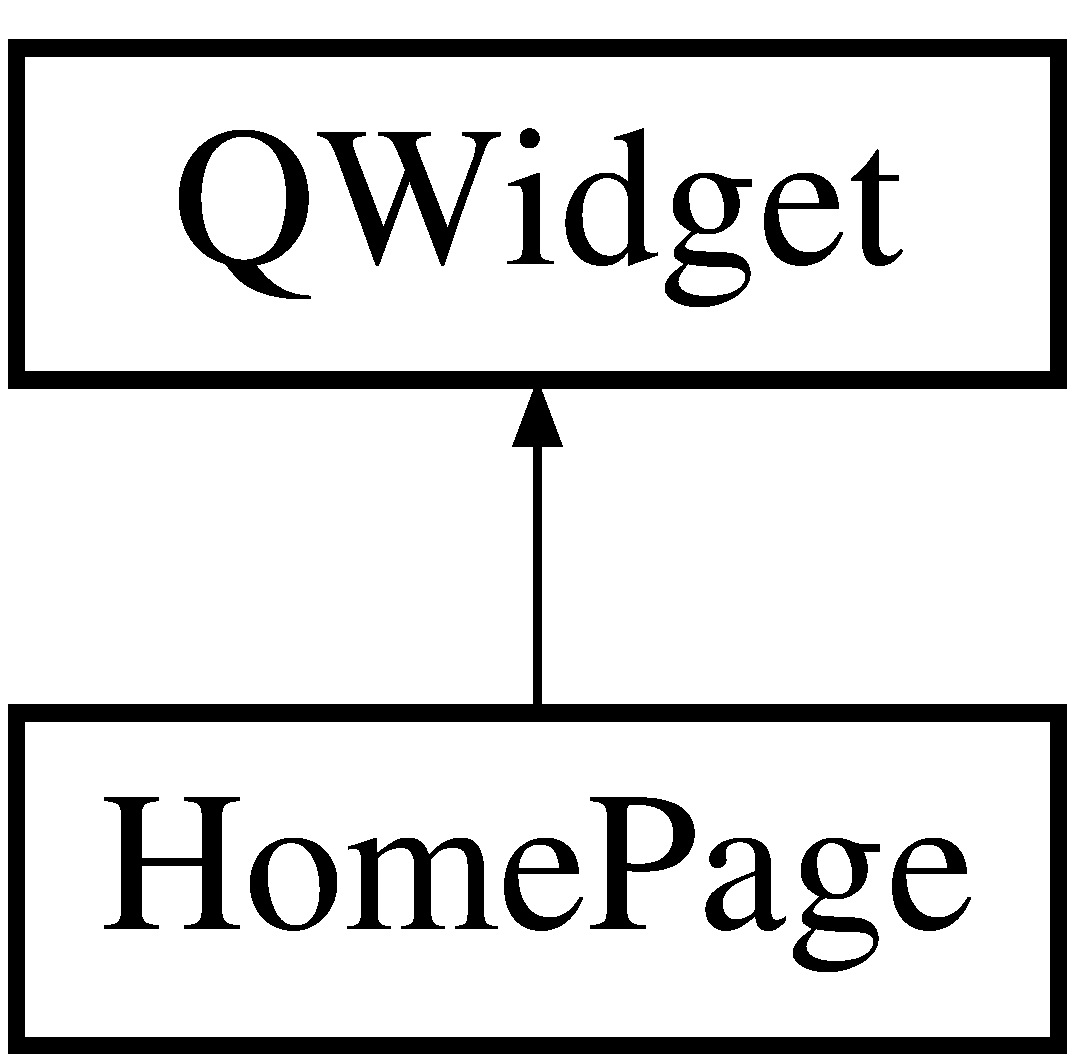
\includegraphics[height=2.000000cm]{class_home_page}
\end{center}
\end{figure}
\subsection*{Signals}
\begin{DoxyCompactItemize}
\item 
void \hyperlink{class_home_page_a0805e5aca6250bd27c2b91459245aaf2}{is\+Finished} (bool)
\end{DoxyCompactItemize}
\subsection*{Public Member Functions}
\begin{DoxyCompactItemize}
\item 
\hyperlink{class_home_page_a11aaf93fd8a54885cf046c23501a07aa}{Home\+Page} (Q\+Widget $\ast$parent=0)
\item 
\hyperlink{class_home_page_aff8e741021104752949c6935c7407f90}{$\sim$\+Home\+Page} ()
\end{DoxyCompactItemize}


\subsection{Detailed Description}


Definition at line 10 of file homepage.\+h.



\subsection{Constructor \& Destructor Documentation}
\index{Home\+Page@{Home\+Page}!Home\+Page@{Home\+Page}}
\index{Home\+Page@{Home\+Page}!Home\+Page@{Home\+Page}}
\subsubsection[{\texorpdfstring{Home\+Page(\+Q\+Widget $\ast$parent=0)}{HomePage(QWidget *parent=0)}}]{\setlength{\rightskip}{0pt plus 5cm}Home\+Page\+::\+Home\+Page (
\begin{DoxyParamCaption}
\item[{Q\+Widget $\ast$}]{parent = {\ttfamily 0}}
\end{DoxyParamCaption}
)\hspace{0.3cm}{\ttfamily [explicit]}}\hypertarget{class_home_page_a11aaf93fd8a54885cf046c23501a07aa}{}\label{class_home_page_a11aaf93fd8a54885cf046c23501a07aa}


Definition at line 7 of file homepage.\+cpp.

\index{Home\+Page@{Home\+Page}!````~Home\+Page@{$\sim$\+Home\+Page}}
\index{````~Home\+Page@{$\sim$\+Home\+Page}!Home\+Page@{Home\+Page}}
\subsubsection[{\texorpdfstring{$\sim$\+Home\+Page()}{~HomePage()}}]{\setlength{\rightskip}{0pt plus 5cm}Home\+Page\+::$\sim$\+Home\+Page (
\begin{DoxyParamCaption}
{}
\end{DoxyParamCaption}
)}\hypertarget{class_home_page_aff8e741021104752949c6935c7407f90}{}\label{class_home_page_aff8e741021104752949c6935c7407f90}


Definition at line 24 of file homepage.\+cpp.



\subsection{Member Function Documentation}
\index{Home\+Page@{Home\+Page}!is\+Finished@{is\+Finished}}
\index{is\+Finished@{is\+Finished}!Home\+Page@{Home\+Page}}
\subsubsection[{\texorpdfstring{is\+Finished}{isFinished}}]{\setlength{\rightskip}{0pt plus 5cm}void Home\+Page\+::is\+Finished (
\begin{DoxyParamCaption}
\item[{bool}]{}
\end{DoxyParamCaption}
)\hspace{0.3cm}{\ttfamily [signal]}}\hypertarget{class_home_page_a0805e5aca6250bd27c2b91459245aaf2}{}\label{class_home_page_a0805e5aca6250bd27c2b91459245aaf2}


The documentation for this class was generated from the following files\+:\begin{DoxyCompactItemize}
\item 
src/header/\hyperlink{homepage_8h}{homepage.\+h}\item 
src/source/\hyperlink{homepage_8cpp}{homepage.\+cpp}\end{DoxyCompactItemize}

\hypertarget{class_index_out_of_bounds}{}\section{Index\+Out\+Of\+Bounds Class Reference}
\label{class_index_out_of_bounds}\index{Index\+Out\+Of\+Bounds@{Index\+Out\+Of\+Bounds}}


{\ttfamily \#include $<$Exceptions.\+h$>$}

Inheritance diagram for Index\+Out\+Of\+Bounds\+:\begin{figure}[H]
\begin{center}
\leavevmode
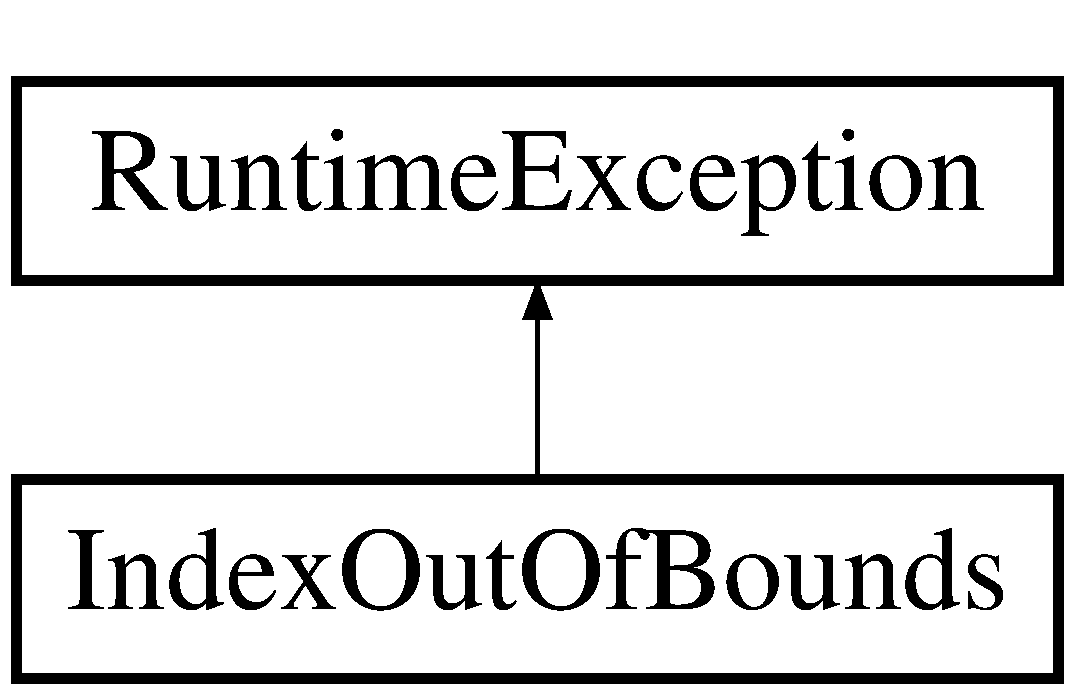
\includegraphics[height=2.000000cm]{class_index_out_of_bounds}
\end{center}
\end{figure}
\subsection*{Public Member Functions}
\begin{DoxyCompactItemize}
\item 
\hyperlink{class_index_out_of_bounds_ac7f448aef9aeaeadef56ed81a30ad8ff}{Index\+Out\+Of\+Bounds} (const std\+::string \&err)
\begin{DoxyCompactList}\small\item\em Create an \hyperlink{class_index_out_of_bounds}{Index\+Out\+Of\+Bounds} exception with a custom error message. \end{DoxyCompactList}\end{DoxyCompactItemize}
\subsection*{Additional Inherited Members}


\subsection{Detailed Description}
An exception class for \hyperlink{class_index_out_of_bounds}{Index\+Out\+Of\+Bounds} errors \begin{DoxyAuthor}{Author}
Jesse Mazzella 
\end{DoxyAuthor}


Definition at line 45 of file Exceptions.\+h.



\subsection{Constructor \& Destructor Documentation}
\index{Index\+Out\+Of\+Bounds@{Index\+Out\+Of\+Bounds}!Index\+Out\+Of\+Bounds@{Index\+Out\+Of\+Bounds}}
\index{Index\+Out\+Of\+Bounds@{Index\+Out\+Of\+Bounds}!Index\+Out\+Of\+Bounds@{Index\+Out\+Of\+Bounds}}
\subsubsection[{\texorpdfstring{Index\+Out\+Of\+Bounds(const std\+::string \&err)}{IndexOutOfBounds(const std::string &err)}}]{\setlength{\rightskip}{0pt plus 5cm}Index\+Out\+Of\+Bounds\+::\+Index\+Out\+Of\+Bounds (
\begin{DoxyParamCaption}
\item[{const std\+::string \&}]{err}
\end{DoxyParamCaption}
)\hspace{0.3cm}{\ttfamily [inline]}}\hypertarget{class_index_out_of_bounds_ac7f448aef9aeaeadef56ed81a30ad8ff}{}\label{class_index_out_of_bounds_ac7f448aef9aeaeadef56ed81a30ad8ff}


Create an \hyperlink{class_index_out_of_bounds}{Index\+Out\+Of\+Bounds} exception with a custom error message. 



Definition at line 50 of file Exceptions.\+h.



The documentation for this class was generated from the following file\+:\begin{DoxyCompactItemize}
\item 
src/header/\hyperlink{_exceptions_8h}{Exceptions.\+h}\end{DoxyCompactItemize}

\hypertarget{struct_q_list_data_1_1_indirect_layout}{}\section{Q\+List\+Data\+:\+:Indirect\+Layout Struct Reference}
\label{struct_q_list_data_1_1_indirect_layout}\index{Q\+List\+Data\+::\+Indirect\+Layout@{Q\+List\+Data\+::\+Indirect\+Layout}}


{\ttfamily \#include $<$qlist.\+h$>$}

Inheritance diagram for Q\+List\+Data\+:\+:Indirect\+Layout\+:\begin{figure}[H]
\begin{center}
\leavevmode
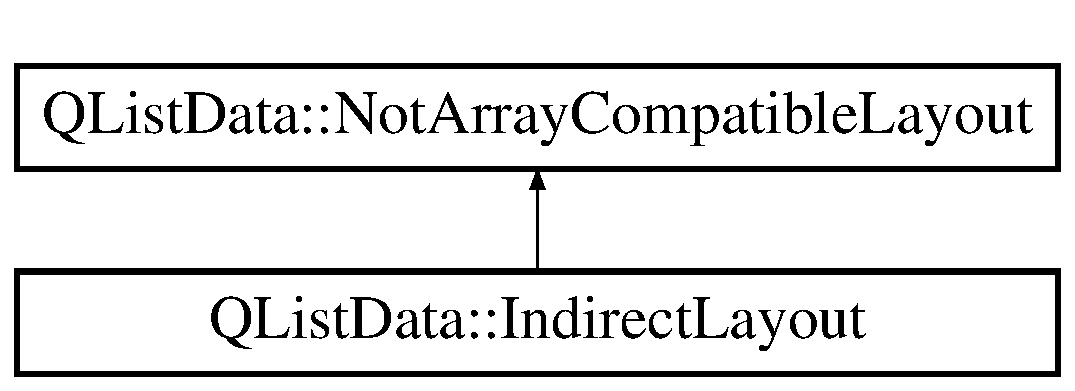
\includegraphics[height=2.000000cm]{struct_q_list_data_1_1_indirect_layout}
\end{center}
\end{figure}


\subsection{Detailed Description}


Definition at line 80 of file qlist.\+h.



The documentation for this struct was generated from the following file\+:\begin{DoxyCompactItemize}
\item 
docs/extra-\/files/\hyperlink{qlist_8h}{qlist.\+h}\end{DoxyCompactItemize}

\hypertarget{struct_q_list_data_1_1_inline_with_padding_layout}{}\section{Q\+List\+Data\+:\+:Inline\+With\+Padding\+Layout Struct Reference}
\label{struct_q_list_data_1_1_inline_with_padding_layout}\index{Q\+List\+Data\+::\+Inline\+With\+Padding\+Layout@{Q\+List\+Data\+::\+Inline\+With\+Padding\+Layout}}


{\ttfamily \#include $<$qlist.\+h$>$}

Inheritance diagram for Q\+List\+Data\+:\+:Inline\+With\+Padding\+Layout\+:\begin{figure}[H]
\begin{center}
\leavevmode
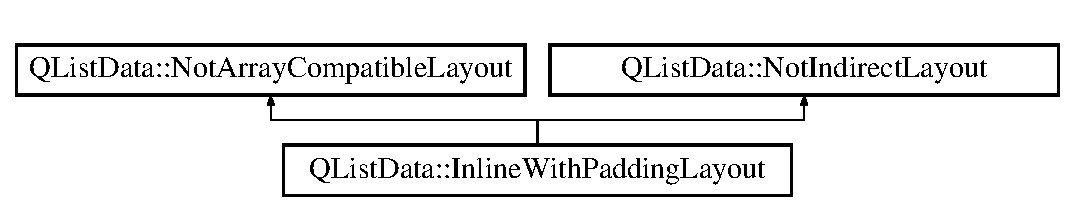
\includegraphics[height=2.000000cm]{struct_q_list_data_1_1_inline_with_padding_layout}
\end{center}
\end{figure}


\subsection{Detailed Description}


Definition at line 79 of file qlist.\+h.



The documentation for this struct was generated from the following file\+:\begin{DoxyCompactItemize}
\item 
docs/extra-\/files/\hyperlink{qlist_8h}{qlist.\+h}\end{DoxyCompactItemize}

\hypertarget{class_q_map_1_1iterator}{}\section{Q\+Map$<$ Key, T $>$\+:\+:iterator Class Reference}
\label{class_q_map_1_1iterator}\index{Q\+Map$<$ Key, T $>$\+::iterator@{Q\+Map$<$ Key, T $>$\+::iterator}}


The \hyperlink{class_q_map_1_1iterator}{Q\+Map\+::iterator} class provides an S\+T\+L-\/style non-\/const iterator for \hyperlink{class_q_map}{Q\+Map} and \hyperlink{class_q_multi_map}{Q\+Multi\+Map}.  




{\ttfamily \#include $<$qmap.\+h$>$}

\subsection*{Public Types}
\begin{DoxyCompactItemize}
\item 
typedef std\+::bidirectional\+\_\+iterator\+\_\+tag \hyperlink{class_q_map_1_1iterator_aade380a34ce9c85a059175d414dbcc92}{iterator\+\_\+category}
\item 
typedef qptrdiff \hyperlink{class_q_map_1_1iterator_afe73281b3461d1635bfdfa5b2e8e7f28}{difference\+\_\+type}
\item 
typedef T \hyperlink{class_q_map_1_1iterator_a7f09aa326409d6d6a02a9a4b4afe3106}{value\+\_\+type}
\item 
typedef T $\ast$ \hyperlink{class_q_map_1_1iterator_ab385357a5b2a2018f1cfa855da8e9285}{pointer}
\item 
typedef T \& \hyperlink{class_q_map_1_1iterator_a51f731d0504f52859c209e708567f0ca}{reference}
\end{DoxyCompactItemize}
\subsection*{Public Member Functions}
\begin{DoxyCompactItemize}
\item 
\hyperlink{class_q_map_1_1iterator_ac7abc795f672ac4049726570ba460c87}{iterator} ()
\item 
\hyperlink{class_q_map_1_1iterator_a3c0ef7bb43edd14e972bcf9649b5649d}{iterator} (\hyperlink{struct_q_map_node}{Node} $\ast$node)
\item 
const Key \& \hyperlink{class_q_map_1_1iterator_af0dfe1fb8fe0c14b209b42f836ef2ee4}{key} () const 
\item 
T \& \hyperlink{class_q_map_1_1iterator_add56d9970fa4c0bb2ffa84fb95a4aa46}{value} () const 
\item 
T \& \hyperlink{class_q_map_1_1iterator_a026751b88c480310a7dfc08c7edc1b16}{operator$\ast$} () const 
\item 
T $\ast$ \hyperlink{class_q_map_1_1iterator_a2bd3c3b35f5d78bb1870c846cdc566d1}{operator-\/$>$} () const 
\item 
bool \hyperlink{class_q_map_1_1iterator_a934510c8ca578b3659b2e91481dd5915}{operator==} (const \hyperlink{class_q_map_1_1iterator}{iterator} \&o) const 
\item 
bool \hyperlink{class_q_map_1_1iterator_a580abd11bf77a6ff8c2cf66c31dac35b}{operator!=} (const \hyperlink{class_q_map_1_1iterator}{iterator} \&o) const 
\item 
\hyperlink{class_q_map_1_1iterator}{iterator} \& \hyperlink{class_q_map_1_1iterator_a119ae3335f65b9d40af561352530e5b8}{operator++} ()
\item 
\hyperlink{class_q_map_1_1iterator}{iterator} \hyperlink{class_q_map_1_1iterator_a9a7434d417ace45b1e55768e2e76f8e3}{operator++} (int)
\item 
\hyperlink{class_q_map_1_1iterator}{iterator} \& \hyperlink{class_q_map_1_1iterator_a9f8068b336d1572a914c4c55d57fc174}{operator-\/-\/} ()
\item 
\hyperlink{class_q_map_1_1iterator}{iterator} \hyperlink{class_q_map_1_1iterator_ac9d9b8e0632050e007466efb2a0764c8}{operator-\/-\/} (int)
\item 
\hyperlink{class_q_map_1_1iterator}{iterator} \hyperlink{class_q_map_1_1iterator_a771aee188731919b54f1dd8e39c2a9cd}{operator+} (int j) const 
\item 
\hyperlink{class_q_map_1_1iterator}{iterator} \hyperlink{class_q_map_1_1iterator_a367af4b10d274f42dfe5b185cf775376}{operator-\/} (int j) const 
\item 
\hyperlink{class_q_map_1_1iterator}{iterator} \& \hyperlink{class_q_map_1_1iterator_a7e809c091ec3533242bcab277fcd1c23}{operator+=} (int j)
\item 
\hyperlink{class_q_map_1_1iterator}{iterator} \& \hyperlink{class_q_map_1_1iterator_abba119aac7555f93740494a1d08de88e}{operator-\/=} (int j)
\item 
bool \hyperlink{class_q_map_1_1iterator_a2a58be489f05e2c1f2b7e1c348b1913d}{operator==} (const \hyperlink{class_q_map_1_1const__iterator}{const\+\_\+iterator} \&o) const 
\item 
bool \hyperlink{class_q_map_1_1iterator_adb5abeeefa73991af41e5d63de0077f5}{operator!=} (const \hyperlink{class_q_map_1_1const__iterator}{const\+\_\+iterator} \&o) const 
\end{DoxyCompactItemize}
\subsection*{Friends}
\begin{DoxyCompactItemize}
\item 
class \hyperlink{class_q_map_1_1iterator_ac220ce1c155db1ac44146c12d178056f}{const\+\_\+iterator}
\item 
class \hyperlink{class_q_map_1_1iterator_a6f07e70412dd8d995969c9e0cb5bc4a0}{Q\+Map$<$ Key, T $>$}
\end{DoxyCompactItemize}


\subsection{Detailed Description}
\subsubsection*{template$<$class Key, class T$>$\\*
class Q\+Map$<$ Key, T $>$\+::iterator}

The \hyperlink{class_q_map_1_1iterator}{Q\+Map\+::iterator} class provides an S\+T\+L-\/style non-\/const iterator for \hyperlink{class_q_map}{Q\+Map} and \hyperlink{class_q_multi_map}{Q\+Multi\+Map}. 

Qt\+Core \hyperlink{class_q_map}{Q\+Map} features both \{S\+T\+L-\/style iterators\} and \{Java-\/style iterators\}. The S\+T\+L-\/style iterators are more low-\/level and more cumbersome to use; on the other hand, they are slightly faster and, for developers who already know S\+TL, have the advantage of familiarity.

\hyperlink{class_q_map}{Q\+Map}$<$Key, T$>$\+::iterator allows you to iterate over a \hyperlink{class_q_map}{Q\+Map} (or \hyperlink{class_q_multi_map}{Q\+Multi\+Map}) and to modify the value (but not the key) stored under a particular key. If you want to iterate over a const \hyperlink{class_q_map}{Q\+Map}, you should use \hyperlink{class_q_map_1_1const__iterator}{Q\+Map\+::const\+\_\+iterator}. It is generally good practice to use \hyperlink{class_q_map_1_1const__iterator}{Q\+Map\+::const\+\_\+iterator} on a non-\/const \hyperlink{class_q_map}{Q\+Map} as well, unless you need to change the \hyperlink{class_q_map}{Q\+Map} through the iterator. Const iterators are slightly faster, and can improve code readability.

The default \hyperlink{class_q_map_1_1iterator}{Q\+Map\+::iterator} constructor creates an uninitialized iterator. You must initialize it using a \hyperlink{class_q_map}{Q\+Map} function like \hyperlink{class_q_map_a5712fc69379f2b6d707a1c65391ff9ef}{Q\+Map\+::begin()}, \hyperlink{class_q_map_a2935881385191efbb074e96cf8d3c9b6}{Q\+Map\+::end()}, or \hyperlink{class_q_map_a8cf44b635018eb178cc724ed20379d85}{Q\+Map\+::find()} before you can start iterating. Here\textquotesingle{}s a typical loop that prints all the (key, value) pairs stored in a map\+:


\begin{DoxyCodeInclude}
\end{DoxyCodeInclude}
 Unlike Q\+Hash, which stores its items in an arbitrary order, \hyperlink{class_q_map}{Q\+Map} stores its items ordered by key. Items that share the same key (because they were inserted using \hyperlink{class_q_map_a075634da2cf912a20dd1c4a5835acfa3}{Q\+Map\+::insert\+Multi()}, or due to a \hyperlink{class_q_map_a4626753159700253f441ad14fdc12245}{unite()}) will appear consecutively, from the most recently to the least recently inserted value.

Let\textquotesingle{}s see a few examples of things we can do with a \hyperlink{class_q_map_1_1iterator}{Q\+Map\+::iterator} that we cannot do with a \hyperlink{class_q_map_1_1const__iterator}{Q\+Map\+::const\+\_\+iterator}. Here\textquotesingle{}s an example that increments every value stored in the \hyperlink{class_q_map}{Q\+Map} by 2\+:


\begin{DoxyCodeInclude}
\end{DoxyCodeInclude}
 Here\textquotesingle{}s an example that removes all the items whose key is a string that starts with an underscore character\+:


\begin{DoxyCodeInclude}
\end{DoxyCodeInclude}
 The call to \hyperlink{class_q_map_add6cad4f0b12644cfe593d95f7a75807}{Q\+Map\+::erase()} removes the item pointed to by the iterator from the map, and returns an iterator to the next item. Here\textquotesingle{}s another way of removing an item while iterating\+:


\begin{DoxyCodeInclude}
\end{DoxyCodeInclude}
 It might be tempting to write code like this\+:


\begin{DoxyCodeInclude}
\end{DoxyCodeInclude}
 However, this will potentially crash in {\ttfamily }\{++i\}, because {\ttfamily i} is a dangling iterator after the call to \hyperlink{class_q_map_add6cad4f0b12644cfe593d95f7a75807}{erase()}.

Multiple iterators can be used on the same map. If you add items to the map, existing iterators will remain valid. If you remove items from the map, iterators that point to the removed items will become dangling iterators.

\begin{DoxyWarning}{Warning}
Iterators on implicitly shared containers do not work exactly like S\+T\+L-\/iterators. You should avoid copying a container while iterators are active on that container. For more information, read \{Implicit sharing iterator problem\}.
\end{DoxyWarning}
\begin{DoxySeeAlso}{See also}
\hyperlink{class_q_map_1_1const__iterator}{Q\+Map\+::const\+\_\+iterator}, Q\+Mutable\+Map\+Iterator 
\end{DoxySeeAlso}


Definition at line 407 of file qmap.\+h.



\subsection{Member Typedef Documentation}
\index{Q\+Map\+::iterator@{Q\+Map\+::iterator}!difference\+\_\+type@{difference\+\_\+type}}
\index{difference\+\_\+type@{difference\+\_\+type}!Q\+Map\+::iterator@{Q\+Map\+::iterator}}
\subsubsection[{\texorpdfstring{difference\+\_\+type}{difference_type}}]{\setlength{\rightskip}{0pt plus 5cm}template$<$class Key, class T$>$ {\bf Q\+Map}$<$ Key, T $>$\+::{\bf iterator\+::difference\+\_\+type}}\hypertarget{class_q_map_1_1iterator_afe73281b3461d1635bfdfa5b2e8e7f28}{}\label{class_q_map_1_1iterator_afe73281b3461d1635bfdfa5b2e8e7f28}


Definition at line 414 of file qmap.\+h.

\index{Q\+Map\+::iterator@{Q\+Map\+::iterator}!iterator\+\_\+category@{iterator\+\_\+category}}
\index{iterator\+\_\+category@{iterator\+\_\+category}!Q\+Map\+::iterator@{Q\+Map\+::iterator}}
\subsubsection[{\texorpdfstring{iterator\+\_\+category}{iterator_category}}]{\setlength{\rightskip}{0pt plus 5cm}template$<$class Key, class T$>$ {\bf Q\+Map}$<$ Key, T $>$\+::{\bf iterator\+::iterator\+\_\+category}}\hypertarget{class_q_map_1_1iterator_aade380a34ce9c85a059175d414dbcc92}{}\label{class_q_map_1_1iterator_aade380a34ce9c85a059175d414dbcc92}
A synonym for {\itshape \{std\+::bidirectional\+\_\+iterator\+\_\+tag\}} indicating this iterator is a bidirectional iterator. 

Definition at line 413 of file qmap.\+h.

\index{Q\+Map\+::iterator@{Q\+Map\+::iterator}!pointer@{pointer}}
\index{pointer@{pointer}!Q\+Map\+::iterator@{Q\+Map\+::iterator}}
\subsubsection[{\texorpdfstring{pointer}{pointer}}]{\setlength{\rightskip}{0pt plus 5cm}template$<$class Key, class T$>$ {\bf Q\+Map}$<$ Key, T $>$\+::{\bf iterator\+::pointer}}\hypertarget{class_q_map_1_1iterator_ab385357a5b2a2018f1cfa855da8e9285}{}\label{class_q_map_1_1iterator_ab385357a5b2a2018f1cfa855da8e9285}


Definition at line 416 of file qmap.\+h.

\index{Q\+Map\+::iterator@{Q\+Map\+::iterator}!reference@{reference}}
\index{reference@{reference}!Q\+Map\+::iterator@{Q\+Map\+::iterator}}
\subsubsection[{\texorpdfstring{reference}{reference}}]{\setlength{\rightskip}{0pt plus 5cm}template$<$class Key, class T$>$ {\bf Q\+Map}$<$ Key, T $>$\+::{\bf iterator\+::reference}}\hypertarget{class_q_map_1_1iterator_a51f731d0504f52859c209e708567f0ca}{}\label{class_q_map_1_1iterator_a51f731d0504f52859c209e708567f0ca}


Definition at line 417 of file qmap.\+h.

\index{Q\+Map\+::iterator@{Q\+Map\+::iterator}!value\+\_\+type@{value\+\_\+type}}
\index{value\+\_\+type@{value\+\_\+type}!Q\+Map\+::iterator@{Q\+Map\+::iterator}}
\subsubsection[{\texorpdfstring{value\+\_\+type}{value_type}}]{\setlength{\rightskip}{0pt plus 5cm}template$<$class Key, class T$>$ {\bf Q\+Map}$<$ Key, T $>$\+::{\bf iterator\+::value\+\_\+type}}\hypertarget{class_q_map_1_1iterator_a7f09aa326409d6d6a02a9a4b4afe3106}{}\label{class_q_map_1_1iterator_a7f09aa326409d6d6a02a9a4b4afe3106}


Definition at line 415 of file qmap.\+h.



\subsection{Constructor \& Destructor Documentation}
\index{Q\+Map\+::iterator@{Q\+Map\+::iterator}!iterator@{iterator}}
\index{iterator@{iterator}!Q\+Map\+::iterator@{Q\+Map\+::iterator}}
\subsubsection[{\texorpdfstring{iterator()}{iterator()}}]{\setlength{\rightskip}{0pt plus 5cm}template$<$class Key, class T$>$ {\bf Q\+Map}$<$ Key, T $>$\+::iterator\+::iterator (
\begin{DoxyParamCaption}
{}
\end{DoxyParamCaption}
)\hspace{0.3cm}{\ttfamily [inline]}}\hypertarget{class_q_map_1_1iterator_ac7abc795f672ac4049726570ba460c87}{}\label{class_q_map_1_1iterator_ac7abc795f672ac4049726570ba460c87}
Constructs an uninitialized iterator.

Functions like \hyperlink{class_q_map_1_1iterator_af0dfe1fb8fe0c14b209b42f836ef2ee4}{key()}, \hyperlink{class_q_map_1_1iterator_add56d9970fa4c0bb2ffa84fb95a4aa46}{value()}, and \hyperlink{class_q_map_1_1iterator_a119ae3335f65b9d40af561352530e5b8}{operator++()} must not be called on an uninitialized iterator. Use \hyperlink{class_q_map_ad04759cfb5b1ed0f3d35a2a16f45ae54}{operator=()} to assign a value to it before using it.

\begin{DoxySeeAlso}{See also}
\hyperlink{class_q_map_a5712fc69379f2b6d707a1c65391ff9ef}{Q\+Map\+::begin()}, \hyperlink{class_q_map_a2935881385191efbb074e96cf8d3c9b6}{Q\+Map\+::end()} 
\end{DoxySeeAlso}


Definition at line 419 of file qmap.\+h.

\index{Q\+Map\+::iterator@{Q\+Map\+::iterator}!iterator@{iterator}}
\index{iterator@{iterator}!Q\+Map\+::iterator@{Q\+Map\+::iterator}}
\subsubsection[{\texorpdfstring{iterator(\+Node $\ast$node)}{iterator(Node *node)}}]{\setlength{\rightskip}{0pt plus 5cm}template$<$class Key, class T$>$ {\bf Q\+Map}$<$ Key, T $>$\+::iterator\+::iterator (
\begin{DoxyParamCaption}
\item[{{\bf Node} $\ast$}]{node}
\end{DoxyParamCaption}
)\hspace{0.3cm}{\ttfamily [inline]}}\hypertarget{class_q_map_1_1iterator_a3c0ef7bb43edd14e972bcf9649b5649d}{}\label{class_q_map_1_1iterator_a3c0ef7bb43edd14e972bcf9649b5649d}


Definition at line 420 of file qmap.\+h.



\subsection{Member Function Documentation}
\index{Q\+Map\+::iterator@{Q\+Map\+::iterator}!key@{key}}
\index{key@{key}!Q\+Map\+::iterator@{Q\+Map\+::iterator}}
\subsubsection[{\texorpdfstring{key() const }{key() const }}]{\setlength{\rightskip}{0pt plus 5cm}template$<$class Key, class T$>$ const Key \& {\bf Q\+Map}$<$ Key, T $>$\+::iterator\+::key (
\begin{DoxyParamCaption}
{}
\end{DoxyParamCaption}
) const\hspace{0.3cm}{\ttfamily [inline]}}\hypertarget{class_q_map_1_1iterator_af0dfe1fb8fe0c14b209b42f836ef2ee4}{}\label{class_q_map_1_1iterator_af0dfe1fb8fe0c14b209b42f836ef2ee4}
Returns the current item\textquotesingle{}s key as a const reference.

There is no direct way of changing an item\textquotesingle{}s key through an iterator, although it can be done by calling \hyperlink{class_q_map_add6cad4f0b12644cfe593d95f7a75807}{Q\+Map\+::erase()} followed by \hyperlink{class_q_map_a0cc56ab47ea14af1127ac7399814d289}{Q\+Map\+::insert()} or \hyperlink{class_q_map_a075634da2cf912a20dd1c4a5835acfa3}{Q\+Map\+::insert\+Multi()}.

\begin{DoxySeeAlso}{See also}
\hyperlink{class_q_map_1_1iterator_add56d9970fa4c0bb2ffa84fb95a4aa46}{value()} 
\end{DoxySeeAlso}


Definition at line 422 of file qmap.\+h.

\index{Q\+Map\+::iterator@{Q\+Map\+::iterator}!operator"!=@{operator"!=}}
\index{operator"!=@{operator"!=}!Q\+Map\+::iterator@{Q\+Map\+::iterator}}
\subsubsection[{\texorpdfstring{operator"!=(const iterator \&o) const }{operator!=(const iterator &o) const }}]{\setlength{\rightskip}{0pt plus 5cm}template$<$class Key, class T$>$ bool {\bf Q\+Map}$<$ Key, T $>$\+::iterator\+::operator!= (
\begin{DoxyParamCaption}
\item[{const {\bf iterator} \&}]{o}
\end{DoxyParamCaption}
) const\hspace{0.3cm}{\ttfamily [inline]}}\hypertarget{class_q_map_1_1iterator_a580abd11bf77a6ff8c2cf66c31dac35b}{}\label{class_q_map_1_1iterator_a580abd11bf77a6ff8c2cf66c31dac35b}


Definition at line 427 of file qmap.\+h.

\index{Q\+Map\+::iterator@{Q\+Map\+::iterator}!operator"!=@{operator"!=}}
\index{operator"!=@{operator"!=}!Q\+Map\+::iterator@{Q\+Map\+::iterator}}
\subsubsection[{\texorpdfstring{operator"!=(const const\+\_\+iterator \&o) const }{operator!=(const const_iterator &o) const }}]{\setlength{\rightskip}{0pt plus 5cm}template$<$class Key, class T$>$ bool {\bf Q\+Map}$<$ Key, T $>$\+::iterator\+::operator!= (
\begin{DoxyParamCaption}
\item[{const {\bf const\+\_\+iterator} \&}]{other}
\end{DoxyParamCaption}
) const\hspace{0.3cm}{\ttfamily [inline]}}\hypertarget{class_q_map_1_1iterator_adb5abeeefa73991af41e5d63de0077f5}{}\label{class_q_map_1_1iterator_adb5abeeefa73991af41e5d63de0077f5}
Returns {\ttfamily true} if {\itshape other} points to a different item than this iterator; otherwise returns {\ttfamily false}.

\begin{DoxySeeAlso}{See also}
\hyperlink{class_q_map_1_1iterator_a934510c8ca578b3659b2e91481dd5915}{operator==()} 
\end{DoxySeeAlso}


Definition at line 457 of file qmap.\+h.

\index{Q\+Map\+::iterator@{Q\+Map\+::iterator}!operator$\ast$@{operator$\ast$}}
\index{operator$\ast$@{operator$\ast$}!Q\+Map\+::iterator@{Q\+Map\+::iterator}}
\subsubsection[{\texorpdfstring{operator$\ast$() const }{operator*() const }}]{\setlength{\rightskip}{0pt plus 5cm}template$<$class Key, class T$>$ T \& {\bf Q\+Map}$<$ Key, T $>$\+::iterator\+::operator$\ast$ (
\begin{DoxyParamCaption}
{}
\end{DoxyParamCaption}
) const\hspace{0.3cm}{\ttfamily [inline]}}\hypertarget{class_q_map_1_1iterator_a026751b88c480310a7dfc08c7edc1b16}{}\label{class_q_map_1_1iterator_a026751b88c480310a7dfc08c7edc1b16}
Returns a modifiable reference to the current item\textquotesingle{}s value.

Same as \hyperlink{class_q_map_1_1iterator_add56d9970fa4c0bb2ffa84fb95a4aa46}{value()}.

\begin{DoxySeeAlso}{See also}
\hyperlink{class_q_map_1_1iterator_af0dfe1fb8fe0c14b209b42f836ef2ee4}{key()} 
\end{DoxySeeAlso}


Definition at line 424 of file qmap.\+h.

\index{Q\+Map\+::iterator@{Q\+Map\+::iterator}!operator+@{operator+}}
\index{operator+@{operator+}!Q\+Map\+::iterator@{Q\+Map\+::iterator}}
\subsubsection[{\texorpdfstring{operator+(int j) const }{operator+(int j) const }}]{\setlength{\rightskip}{0pt plus 5cm}template$<$class Key, class T$>$ {\bf Q\+Map\+::iterator} {\bf Q\+Map}$<$ Key, T $>$\+::iterator\+::operator+ (
\begin{DoxyParamCaption}
\item[{int}]{j}
\end{DoxyParamCaption}
) const\hspace{0.3cm}{\ttfamily [inline]}}\hypertarget{class_q_map_1_1iterator_a771aee188731919b54f1dd8e39c2a9cd}{}\label{class_q_map_1_1iterator_a771aee188731919b54f1dd8e39c2a9cd}
Returns an iterator to the item at {\itshape j} positions forward from this iterator. (If {\itshape j} is negative, the iterator goes backward.)

This operation can be slow for large {\itshape j} values.

\begin{DoxySeeAlso}{See also}
\hyperlink{class_q_map_1_1iterator_a367af4b10d274f42dfe5b185cf775376}{operator-\/()} 
\end{DoxySeeAlso}


Definition at line 447 of file qmap.\+h.

\index{Q\+Map\+::iterator@{Q\+Map\+::iterator}!operator++@{operator++}}
\index{operator++@{operator++}!Q\+Map\+::iterator@{Q\+Map\+::iterator}}
\subsubsection[{\texorpdfstring{operator++()}{operator++()}}]{\setlength{\rightskip}{0pt plus 5cm}template$<$class Key, class T$>$ {\bf Q\+Map\+::iterator} {\bf Q\+Map}$<$ Key, T $>$\+::iterator\+::operator++ (
\begin{DoxyParamCaption}
{}
\end{DoxyParamCaption}
)\hspace{0.3cm}{\ttfamily [inline]}}\hypertarget{class_q_map_1_1iterator_a119ae3335f65b9d40af561352530e5b8}{}\label{class_q_map_1_1iterator_a119ae3335f65b9d40af561352530e5b8}
The prefix ++ operator ({\ttfamily }\{++i\}) advances the iterator to the next item in the map and returns an iterator to the new current item.

Calling this function on \hyperlink{class_q_map_a2935881385191efbb074e96cf8d3c9b6}{Q\+Map\+::end()} leads to undefined results.

\begin{DoxySeeAlso}{See also}
\hyperlink{class_q_map_1_1iterator_a9f8068b336d1572a914c4c55d57fc174}{operator-\/-\/()} 
\end{DoxySeeAlso}


Definition at line 429 of file qmap.\+h.

\index{Q\+Map\+::iterator@{Q\+Map\+::iterator}!operator++@{operator++}}
\index{operator++@{operator++}!Q\+Map\+::iterator@{Q\+Map\+::iterator}}
\subsubsection[{\texorpdfstring{operator++(int)}{operator++(int)}}]{\setlength{\rightskip}{0pt plus 5cm}template$<$class Key, class T$>$ {\bf Q\+Map\+::iterator} {\bf Q\+Map}$<$ Key, T $>$\+::iterator\+::operator++ (
\begin{DoxyParamCaption}
\item[{int}]{}
\end{DoxyParamCaption}
)\hspace{0.3cm}{\ttfamily [inline]}}\hypertarget{class_q_map_1_1iterator_a9a7434d417ace45b1e55768e2e76f8e3}{}\label{class_q_map_1_1iterator_a9a7434d417ace45b1e55768e2e76f8e3}
This is an overloaded member function, provided for convenience. It differs from the above function only in what argument(s) it accepts.

The postfix ++ operator ({\ttfamily }\{i++\}) advances the iterator to the next item in the map and returns an iterator to the previously current item. 

Definition at line 433 of file qmap.\+h.

\index{Q\+Map\+::iterator@{Q\+Map\+::iterator}!operator+=@{operator+=}}
\index{operator+=@{operator+=}!Q\+Map\+::iterator@{Q\+Map\+::iterator}}
\subsubsection[{\texorpdfstring{operator+=(int j)}{operator+=(int j)}}]{\setlength{\rightskip}{0pt plus 5cm}template$<$class Key, class T$>$ {\bf Q\+Map\+::iterator} \& {\bf Q\+Map}$<$ Key, T $>$\+::iterator\+::operator+= (
\begin{DoxyParamCaption}
\item[{int}]{j}
\end{DoxyParamCaption}
)\hspace{0.3cm}{\ttfamily [inline]}}\hypertarget{class_q_map_1_1iterator_a7e809c091ec3533242bcab277fcd1c23}{}\label{class_q_map_1_1iterator_a7e809c091ec3533242bcab277fcd1c23}
Advances the iterator by {\itshape j} items. (If {\itshape j} is negative, the iterator goes backward.)

\begin{DoxySeeAlso}{See also}
\hyperlink{class_q_map_1_1iterator_abba119aac7555f93740494a1d08de88e}{operator-\/=()}, \hyperlink{class_q_map_1_1iterator_a771aee188731919b54f1dd8e39c2a9cd}{operator+()} 
\end{DoxySeeAlso}


Definition at line 450 of file qmap.\+h.

\index{Q\+Map\+::iterator@{Q\+Map\+::iterator}!operator-\/@{operator-\/}}
\index{operator-\/@{operator-\/}!Q\+Map\+::iterator@{Q\+Map\+::iterator}}
\subsubsection[{\texorpdfstring{operator-\/(int j) const }{operator-(int j) const }}]{\setlength{\rightskip}{0pt plus 5cm}template$<$class Key, class T$>$ {\bf Q\+Map\+::iterator} {\bf Q\+Map}$<$ Key, T $>$\+::iterator\+::operator-\/ (
\begin{DoxyParamCaption}
\item[{int}]{j}
\end{DoxyParamCaption}
) const\hspace{0.3cm}{\ttfamily [inline]}}\hypertarget{class_q_map_1_1iterator_a367af4b10d274f42dfe5b185cf775376}{}\label{class_q_map_1_1iterator_a367af4b10d274f42dfe5b185cf775376}
Returns an iterator to the item at {\itshape j} positions backward from this iterator. (If {\itshape j} is negative, the iterator goes forward.)

This operation can be slow for large {\itshape j} values.

\begin{DoxySeeAlso}{See also}
\hyperlink{class_q_map_1_1iterator_a771aee188731919b54f1dd8e39c2a9cd}{operator+()} 
\end{DoxySeeAlso}


Definition at line 449 of file qmap.\+h.

\index{Q\+Map\+::iterator@{Q\+Map\+::iterator}!operator-\/-\/@{operator-\/-\/}}
\index{operator-\/-\/@{operator-\/-\/}!Q\+Map\+::iterator@{Q\+Map\+::iterator}}
\subsubsection[{\texorpdfstring{operator-\/-\/()}{operator--()}}]{\setlength{\rightskip}{0pt plus 5cm}template$<$class Key, class T$>$ {\bf Q\+Map\+::iterator} {\bf Q\+Map}$<$ Key, T $>$\+::iterator\+::operator-\/-\/ (
\begin{DoxyParamCaption}
{}
\end{DoxyParamCaption}
)\hspace{0.3cm}{\ttfamily [inline]}}\hypertarget{class_q_map_1_1iterator_a9f8068b336d1572a914c4c55d57fc174}{}\label{class_q_map_1_1iterator_a9f8068b336d1572a914c4c55d57fc174}
The prefix -- operator ({\ttfamily }\{--i\}) makes the preceding item current and returns an iterator pointing to the new current item.

Calling this function on \hyperlink{class_q_map_a5712fc69379f2b6d707a1c65391ff9ef}{Q\+Map\+::begin()} leads to undefined results.

\begin{DoxySeeAlso}{See also}
\hyperlink{class_q_map_1_1iterator_a119ae3335f65b9d40af561352530e5b8}{operator++()} 
\end{DoxySeeAlso}


Definition at line 438 of file qmap.\+h.

\index{Q\+Map\+::iterator@{Q\+Map\+::iterator}!operator-\/-\/@{operator-\/-\/}}
\index{operator-\/-\/@{operator-\/-\/}!Q\+Map\+::iterator@{Q\+Map\+::iterator}}
\subsubsection[{\texorpdfstring{operator-\/-\/(int)}{operator--(int)}}]{\setlength{\rightskip}{0pt plus 5cm}template$<$class Key, class T$>$ {\bf Q\+Map\+::iterator} {\bf Q\+Map}$<$ Key, T $>$\+::iterator\+::operator-\/-\/ (
\begin{DoxyParamCaption}
\item[{int}]{}
\end{DoxyParamCaption}
)\hspace{0.3cm}{\ttfamily [inline]}}\hypertarget{class_q_map_1_1iterator_ac9d9b8e0632050e007466efb2a0764c8}{}\label{class_q_map_1_1iterator_ac9d9b8e0632050e007466efb2a0764c8}
This is an overloaded member function, provided for convenience. It differs from the above function only in what argument(s) it accepts.

The postfix -- operator ({\ttfamily }\{i--\}) makes the preceding item current and returns an iterator pointing to the previously current item. 

Definition at line 442 of file qmap.\+h.

\index{Q\+Map\+::iterator@{Q\+Map\+::iterator}!operator-\/=@{operator-\/=}}
\index{operator-\/=@{operator-\/=}!Q\+Map\+::iterator@{Q\+Map\+::iterator}}
\subsubsection[{\texorpdfstring{operator-\/=(int j)}{operator-=(int j)}}]{\setlength{\rightskip}{0pt plus 5cm}template$<$class Key, class T$>$ {\bf Q\+Map\+::iterator} \& {\bf Q\+Map}$<$ Key, T $>$\+::iterator\+::operator-\/= (
\begin{DoxyParamCaption}
\item[{int}]{j}
\end{DoxyParamCaption}
)\hspace{0.3cm}{\ttfamily [inline]}}\hypertarget{class_q_map_1_1iterator_abba119aac7555f93740494a1d08de88e}{}\label{class_q_map_1_1iterator_abba119aac7555f93740494a1d08de88e}
Makes the iterator go back by {\itshape j} items. (If {\itshape j} is negative, the iterator goes forward.)

\begin{DoxySeeAlso}{See also}
\hyperlink{class_q_map_1_1iterator_a7e809c091ec3533242bcab277fcd1c23}{operator+=()}, \hyperlink{class_q_map_1_1iterator_a367af4b10d274f42dfe5b185cf775376}{operator-\/()} 
\end{DoxySeeAlso}


Definition at line 451 of file qmap.\+h.

\index{Q\+Map\+::iterator@{Q\+Map\+::iterator}!operator-\/$>$@{operator-\/$>$}}
\index{operator-\/$>$@{operator-\/$>$}!Q\+Map\+::iterator@{Q\+Map\+::iterator}}
\subsubsection[{\texorpdfstring{operator-\/$>$() const }{operator->() const }}]{\setlength{\rightskip}{0pt plus 5cm}template$<$class Key, class T$>$ T $\ast$ {\bf Q\+Map}$<$ Key, T $>$\+::iterator\+::operator-\/$>$ (
\begin{DoxyParamCaption}
{}
\end{DoxyParamCaption}
) const\hspace{0.3cm}{\ttfamily [inline]}}\hypertarget{class_q_map_1_1iterator_a2bd3c3b35f5d78bb1870c846cdc566d1}{}\label{class_q_map_1_1iterator_a2bd3c3b35f5d78bb1870c846cdc566d1}
Returns a pointer to the current item\textquotesingle{}s value.

\begin{DoxySeeAlso}{See also}
\hyperlink{class_q_map_1_1iterator_add56d9970fa4c0bb2ffa84fb95a4aa46}{value()} 
\end{DoxySeeAlso}


Definition at line 425 of file qmap.\+h.

\index{Q\+Map\+::iterator@{Q\+Map\+::iterator}!operator==@{operator==}}
\index{operator==@{operator==}!Q\+Map\+::iterator@{Q\+Map\+::iterator}}
\subsubsection[{\texorpdfstring{operator==(const iterator \&o) const }{operator==(const iterator &o) const }}]{\setlength{\rightskip}{0pt plus 5cm}template$<$class Key, class T$>$ bool {\bf Q\+Map}$<$ Key, T $>$\+::iterator\+::operator== (
\begin{DoxyParamCaption}
\item[{const {\bf iterator} \&}]{o}
\end{DoxyParamCaption}
) const\hspace{0.3cm}{\ttfamily [inline]}}\hypertarget{class_q_map_1_1iterator_a934510c8ca578b3659b2e91481dd5915}{}\label{class_q_map_1_1iterator_a934510c8ca578b3659b2e91481dd5915}


Definition at line 426 of file qmap.\+h.

\index{Q\+Map\+::iterator@{Q\+Map\+::iterator}!operator==@{operator==}}
\index{operator==@{operator==}!Q\+Map\+::iterator@{Q\+Map\+::iterator}}
\subsubsection[{\texorpdfstring{operator==(const const\+\_\+iterator \&o) const }{operator==(const const_iterator &o) const }}]{\setlength{\rightskip}{0pt plus 5cm}template$<$class Key, class T$>$ bool {\bf Q\+Map}$<$ Key, T $>$\+::iterator\+::operator== (
\begin{DoxyParamCaption}
\item[{const {\bf const\+\_\+iterator} \&}]{other}
\end{DoxyParamCaption}
) const\hspace{0.3cm}{\ttfamily [inline]}}\hypertarget{class_q_map_1_1iterator_a2a58be489f05e2c1f2b7e1c348b1913d}{}\label{class_q_map_1_1iterator_a2a58be489f05e2c1f2b7e1c348b1913d}
Returns {\ttfamily true} if {\itshape other} points to the same item as this iterator; otherwise returns {\ttfamily false}.

\begin{DoxySeeAlso}{See also}
\hyperlink{class_q_map_1_1iterator_a580abd11bf77a6ff8c2cf66c31dac35b}{operator!=()} 
\end{DoxySeeAlso}


Definition at line 455 of file qmap.\+h.

\index{Q\+Map\+::iterator@{Q\+Map\+::iterator}!value@{value}}
\index{value@{value}!Q\+Map\+::iterator@{Q\+Map\+::iterator}}
\subsubsection[{\texorpdfstring{value() const }{value() const }}]{\setlength{\rightskip}{0pt plus 5cm}template$<$class Key, class T$>$ T \& {\bf Q\+Map}$<$ Key, T $>$\+::iterator\+::value (
\begin{DoxyParamCaption}
{}
\end{DoxyParamCaption}
) const\hspace{0.3cm}{\ttfamily [inline]}}\hypertarget{class_q_map_1_1iterator_add56d9970fa4c0bb2ffa84fb95a4aa46}{}\label{class_q_map_1_1iterator_add56d9970fa4c0bb2ffa84fb95a4aa46}
Returns a modifiable reference to the current item\textquotesingle{}s value.

You can change the value of an item by using \hyperlink{class_q_map_1_1iterator_add56d9970fa4c0bb2ffa84fb95a4aa46}{value()} on the left side of an assignment, for example\+:


\begin{DoxyCodeInclude}
\end{DoxyCodeInclude}
 \begin{DoxySeeAlso}{See also}
\hyperlink{class_q_map_1_1iterator_af0dfe1fb8fe0c14b209b42f836ef2ee4}{key()}, \hyperlink{class_q_map_1_1iterator_a026751b88c480310a7dfc08c7edc1b16}{operator$\ast$()} 
\end{DoxySeeAlso}


Definition at line 423 of file qmap.\+h.



\subsection{Friends And Related Function Documentation}
\index{Q\+Map\+::iterator@{Q\+Map\+::iterator}!const\+\_\+iterator@{const\+\_\+iterator}}
\index{const\+\_\+iterator@{const\+\_\+iterator}!Q\+Map\+::iterator@{Q\+Map\+::iterator}}
\subsubsection[{\texorpdfstring{const\+\_\+iterator}{const_iterator}}]{\setlength{\rightskip}{0pt plus 5cm}template$<$class Key, class T$>$ friend class {\bf const\+\_\+iterator}\hspace{0.3cm}{\ttfamily [friend]}}\hypertarget{class_q_map_1_1iterator_ac220ce1c155db1ac44146c12d178056f}{}\label{class_q_map_1_1iterator_ac220ce1c155db1ac44146c12d178056f}


Definition at line 409 of file qmap.\+h.

\index{Q\+Map\+::iterator@{Q\+Map\+::iterator}!Q\+Map$<$ Key, T $>$@{Q\+Map$<$ Key, T $>$}}
\index{Q\+Map$<$ Key, T $>$@{Q\+Map$<$ Key, T $>$}!Q\+Map\+::iterator@{Q\+Map\+::iterator}}
\subsubsection[{\texorpdfstring{Q\+Map$<$ Key, T $>$}{QMap< Key, T >}}]{\setlength{\rightskip}{0pt plus 5cm}template$<$class Key, class T$>$ friend class {\bf Q\+Map}$<$ Key, T $>$\hspace{0.3cm}{\ttfamily [friend]}}\hypertarget{class_q_map_1_1iterator_a6f07e70412dd8d995969c9e0cb5bc4a0}{}\label{class_q_map_1_1iterator_a6f07e70412dd8d995969c9e0cb5bc4a0}


Definition at line 460 of file qmap.\+h.



The documentation for this class was generated from the following files\+:\begin{DoxyCompactItemize}
\item 
docs/extra-\/files/\hyperlink{qmap_8h}{qmap.\+h}\item 
docs/extra-\/files/\hyperlink{qmap_8cpp}{qmap.\+cpp}\end{DoxyCompactItemize}

\hypertarget{class_q_list_1_1iterator}{}\section{Q\+List$<$ T $>$\+:\+:iterator Class Reference}
\label{class_q_list_1_1iterator}\index{Q\+List$<$ T $>$\+::iterator@{Q\+List$<$ T $>$\+::iterator}}


The \hyperlink{class_q_list_1_1iterator}{Q\+List\+::iterator} class provides an S\+T\+L-\/style non-\/const iterator for \hyperlink{class_q_list}{Q\+List} and Q\+Queue.  




{\ttfamily \#include $<$qlist.\+h$>$}

\subsection*{Public Types}
\begin{DoxyCompactItemize}
\item 
typedef std\+::random\+\_\+access\+\_\+iterator\+\_\+tag \hyperlink{class_q_list_1_1iterator_aef6f10c045692f5c9f82a9a629e76a82}{iterator\+\_\+category}
\item 
typedef qptrdiff \hyperlink{class_q_list_1_1iterator_a6360336f54f546a21d69e233f8334fc5}{difference\+\_\+type}
\item 
typedef T \hyperlink{class_q_list_1_1iterator_aab450769169fdaaabc317ed16833d3fb}{value\+\_\+type}
\item 
typedef T $\ast$ \hyperlink{class_q_list_1_1iterator_a07f26136c3c7f042cce2f522ecf15f17}{pointer}
\item 
typedef T \& \hyperlink{class_q_list_1_1iterator_aadf226cf04225b39acd26973c72681bc}{reference}
\end{DoxyCompactItemize}
\subsection*{Public Member Functions}
\begin{DoxyCompactItemize}
\item 
\hyperlink{class_q_list_1_1iterator_ac2334d3597b063090a5245ec44786436}{iterator} ()
\item 
\hyperlink{class_q_list_1_1iterator_a03dae5ce262e310ef83ed2f9384f3ef5}{iterator} (Node $\ast$n)
\item 
\hyperlink{class_q_list_1_1iterator_a7cb730ca6e7c0553e43f18f66068ac24}{iterator} (const \hyperlink{class_q_list_1_1iterator}{iterator} \&o)
\item 
T \& \hyperlink{class_q_list_1_1iterator_a9cd6d05402cf6ebed3dfd2b727edc2a2}{operator$\ast$} () const 
\item 
T $\ast$ \hyperlink{class_q_list_1_1iterator_aa64e03c9f94250dc82ef865ee7e6c557}{operator-\/$>$} () const 
\item 
T \& \hyperlink{class_q_list_1_1iterator_a960fdd912273a727a6eaf6a4429e98d2}{operator\mbox{[}$\,$\mbox{]}} (\hyperlink{class_q_list_1_1iterator_a6360336f54f546a21d69e233f8334fc5}{difference\+\_\+type} j) const 
\item 
bool \hyperlink{class_q_list_1_1iterator_a75de13cfc3058f4dcd5eaa2aa892d27e}{operator==} (const \hyperlink{class_q_list_1_1iterator}{iterator} \&o) const 
\item 
bool \hyperlink{class_q_list_1_1iterator_a5607c6d4b8de3abfa1860ecf9c8e080c}{operator!=} (const \hyperlink{class_q_list_1_1iterator}{iterator} \&o) const 
\item 
bool \hyperlink{class_q_list_1_1iterator_a5be0a12d51850af28383d1048c8f04c0}{operator$<$} (const \hyperlink{class_q_list_1_1iterator}{iterator} \&other) const 
\item 
bool \hyperlink{class_q_list_1_1iterator_ac793fb6f19517bb7c87b7a7f0bce5c4b}{operator$<$=} (const \hyperlink{class_q_list_1_1iterator}{iterator} \&other) const 
\item 
bool \hyperlink{class_q_list_1_1iterator_a1295ca951b546ccfdd84c89d83bef359}{operator$>$} (const \hyperlink{class_q_list_1_1iterator}{iterator} \&other) const 
\item 
bool \hyperlink{class_q_list_1_1iterator_a9ee24a4a8ba02bc7bd4c08465bbb9abd}{operator$>$=} (const \hyperlink{class_q_list_1_1iterator}{iterator} \&other) const 
\item 
bool \hyperlink{class_q_list_1_1iterator_a7bc9996f3154ce695276731e8d55c33b}{operator==} (const \hyperlink{class_q_list_1_1const__iterator}{const\+\_\+iterator} \&o) const 
\item 
bool \hyperlink{class_q_list_1_1iterator_ab3cfcd15a1b076ca1870d2ca72d72b6a}{operator!=} (const \hyperlink{class_q_list_1_1const__iterator}{const\+\_\+iterator} \&o) const 
\item 
bool \hyperlink{class_q_list_1_1iterator_ada8c924f9a031ca2a6d0533b79478018}{operator$<$} (const \hyperlink{class_q_list_1_1const__iterator}{const\+\_\+iterator} \&other) const 
\item 
bool \hyperlink{class_q_list_1_1iterator_a3a7695c52445c55c001e3b032ee781ab}{operator$<$=} (const \hyperlink{class_q_list_1_1const__iterator}{const\+\_\+iterator} \&other) const 
\item 
bool \hyperlink{class_q_list_1_1iterator_a1942047973479c54ea3554424be4a74b}{operator$>$} (const \hyperlink{class_q_list_1_1const__iterator}{const\+\_\+iterator} \&other) const 
\item 
bool \hyperlink{class_q_list_1_1iterator_abfe3b9e2786ce7ee96d4d269d52f2f64}{operator$>$=} (const \hyperlink{class_q_list_1_1const__iterator}{const\+\_\+iterator} \&other) const 
\item 
\hyperlink{class_q_list_1_1iterator}{iterator} \& \hyperlink{class_q_list_1_1iterator_ad7945f61e486c6a104042f57ced0abc3}{operator++} ()
\item 
\hyperlink{class_q_list_1_1iterator}{iterator} \hyperlink{class_q_list_1_1iterator_aed330ca786943bab5ad53c7647aabdef}{operator++} (int)
\item 
\hyperlink{class_q_list_1_1iterator}{iterator} \& \hyperlink{class_q_list_1_1iterator_a7a5a35f25f1839b985d897464ac2d44e}{operator-\/-\/} ()
\item 
\hyperlink{class_q_list_1_1iterator}{iterator} \hyperlink{class_q_list_1_1iterator_a8b004cb6aea3fe5eead5a2db1fe826b0}{operator-\/-\/} (int)
\item 
\hyperlink{class_q_list_1_1iterator}{iterator} \& \hyperlink{class_q_list_1_1iterator_ac7f1c22e07d7d8d70012bd622cff86d7}{operator+=} (\hyperlink{class_q_list_1_1iterator_a6360336f54f546a21d69e233f8334fc5}{difference\+\_\+type} j)
\item 
\hyperlink{class_q_list_1_1iterator}{iterator} \& \hyperlink{class_q_list_1_1iterator_ab46618ab9d6063adcde81007c79a8d3f}{operator-\/=} (\hyperlink{class_q_list_1_1iterator_a6360336f54f546a21d69e233f8334fc5}{difference\+\_\+type} j)
\item 
\hyperlink{class_q_list_1_1iterator}{iterator} \hyperlink{class_q_list_1_1iterator_abaf2621f9687beef6fb25383c6919cb3}{operator+} (\hyperlink{class_q_list_1_1iterator_a6360336f54f546a21d69e233f8334fc5}{difference\+\_\+type} j) const 
\item 
\hyperlink{class_q_list_1_1iterator}{iterator} \hyperlink{class_q_list_1_1iterator_a1ef9ddcbeb387df3984f74b9588af2e9}{operator-\/} (\hyperlink{class_q_list_1_1iterator_a6360336f54f546a21d69e233f8334fc5}{difference\+\_\+type} j) const 
\item 
int \hyperlink{class_q_list_1_1iterator_a9cc15e0eacc43cfa2017d54d310cf10b}{operator-\/} (\hyperlink{class_q_list_1_1iterator}{iterator} j) const 
\end{DoxyCompactItemize}
\subsection*{Public Attributes}
\begin{DoxyCompactItemize}
\item 
Node $\ast$ \hyperlink{class_q_list_1_1iterator_a47610ba7fcbf05bf63ec1cccc28bce98}{i}
\end{DoxyCompactItemize}


\subsection{Detailed Description}
\subsubsection*{template$<$typename T$>$\\*
class Q\+List$<$ T $>$\+::iterator}

The \hyperlink{class_q_list_1_1iterator}{Q\+List\+::iterator} class provides an S\+T\+L-\/style non-\/const iterator for \hyperlink{class_q_list}{Q\+List} and Q\+Queue. 

Qt\+Core \hyperlink{class_q_list}{Q\+List} features both \{S\+T\+L-\/style iterators\} and \{Java-\/style iterators\}. The S\+T\+L-\/style iterators are more low-\/level and more cumbersome to use; on the other hand, they are slightly faster and, for developers who already know S\+TL, have the advantage of familiarity.

\hyperlink{class_q_list}{Q\+List}$<$T$>$\+::iterator allows you to iterate over a \hyperlink{class_q_list}{Q\+List}$<$T$>$ (or Q\+Queue$<$T$>$) and to modify the list item associated with the iterator. If you want to iterate over a const \hyperlink{class_q_list}{Q\+List}, use \hyperlink{class_q_list_1_1const__iterator}{Q\+List\+::const\+\_\+iterator} instead. It is generally good practice to use \hyperlink{class_q_list_1_1const__iterator}{Q\+List\+::const\+\_\+iterator} on a non-\/const \hyperlink{class_q_list}{Q\+List} as well, unless you need to change the \hyperlink{class_q_list}{Q\+List} through the iterator. Const iterators are slightly faster, and can improve code readability.

The default \hyperlink{class_q_list_1_1iterator}{Q\+List\+::iterator} constructor creates an uninitialized iterator. You must initialize it using a \hyperlink{class_q_list}{Q\+List} function like \hyperlink{class_q_list_a06847e57431af245c937c8cfe1c14761}{Q\+List\+::begin()}, \hyperlink{class_q_list_a5695ddeb676cedece5b061eba08c1d0c}{Q\+List\+::end()}, or \hyperlink{class_q_list_a2ae4b66fdb5875c4c55eb903fa5ca25b}{Q\+List\+::insert()} before you can start iterating. Here\textquotesingle{}s a typical loop that prints all the items stored in a list\+:


\begin{DoxyCodeInclude}
\end{DoxyCodeInclude}
 Let\textquotesingle{}s see a few examples of things we can do with a \hyperlink{class_q_list_1_1iterator}{Q\+List\+::iterator} that we cannot do with a \hyperlink{class_q_list_1_1const__iterator}{Q\+List\+::const\+\_\+iterator}. Here\textquotesingle{}s an example that increments every value stored in a \hyperlink{class_q_list}{Q\+List}$<$int$>$ by 2\+:


\begin{DoxyCodeInclude}
\end{DoxyCodeInclude}
 Most \hyperlink{class_q_list}{Q\+List} functions accept an integer index rather than an iterator. For that reason, iterators are rarely useful in connection with \hyperlink{class_q_list}{Q\+List}. One place where S\+T\+L-\/style iterators do make sense is as arguments to \{generic algorithms\}.

For example, here\textquotesingle{}s how to delete all the widgets stored in a \hyperlink{class_q_list}{Q\+List}$<$Q\+Widget $\ast$$>$\+:


\begin{DoxyCodeInclude}
\end{DoxyCodeInclude}
 Multiple iterators can be used on the same list. However, be aware that any non-\/const function call performed on the \hyperlink{class_q_list}{Q\+List} will render all existing iterators undefined. If you need to keep iterators over a long period of time, we recommend that you use Q\+Linked\+List rather than \hyperlink{class_q_list}{Q\+List}.

\begin{DoxyWarning}{Warning}
Iterators on implicitly shared containers do not work exactly like S\+T\+L-\/iterators. You should avoid copying a container while iterators are active on that container. For more information, read \{Implicit sharing iterator problem\}.
\end{DoxyWarning}
\begin{DoxySeeAlso}{See also}
\hyperlink{class_q_list_1_1const__iterator}{Q\+List\+::const\+\_\+iterator}, Q\+Mutable\+List\+Iterator 
\end{DoxySeeAlso}


Definition at line 211 of file qlist.\+h.



\subsection{Member Typedef Documentation}
\index{Q\+List\+::iterator@{Q\+List\+::iterator}!difference\+\_\+type@{difference\+\_\+type}}
\index{difference\+\_\+type@{difference\+\_\+type}!Q\+List\+::iterator@{Q\+List\+::iterator}}
\subsubsection[{\texorpdfstring{difference\+\_\+type}{difference_type}}]{\setlength{\rightskip}{0pt plus 5cm}template$<$typename T$>$ {\bf Q\+List}$<$ T $>$\+::{\bf iterator\+::difference\+\_\+type}}\hypertarget{class_q_list_1_1iterator_a6360336f54f546a21d69e233f8334fc5}{}\label{class_q_list_1_1iterator_a6360336f54f546a21d69e233f8334fc5}


Definition at line 216 of file qlist.\+h.

\index{Q\+List\+::iterator@{Q\+List\+::iterator}!iterator\+\_\+category@{iterator\+\_\+category}}
\index{iterator\+\_\+category@{iterator\+\_\+category}!Q\+List\+::iterator@{Q\+List\+::iterator}}
\subsubsection[{\texorpdfstring{iterator\+\_\+category}{iterator_category}}]{\setlength{\rightskip}{0pt plus 5cm}template$<$typename T$>$ {\bf Q\+List}$<$ T $>$\+::{\bf iterator\+::iterator\+\_\+category}}\hypertarget{class_q_list_1_1iterator_aef6f10c045692f5c9f82a9a629e76a82}{}\label{class_q_list_1_1iterator_aef6f10c045692f5c9f82a9a629e76a82}
A synonym for {\itshape \{std\+::random\+\_\+access\+\_\+iterator\+\_\+tag\}} indicating this iterator is a random access iterator. 

Definition at line 214 of file qlist.\+h.

\index{Q\+List\+::iterator@{Q\+List\+::iterator}!pointer@{pointer}}
\index{pointer@{pointer}!Q\+List\+::iterator@{Q\+List\+::iterator}}
\subsubsection[{\texorpdfstring{pointer}{pointer}}]{\setlength{\rightskip}{0pt plus 5cm}template$<$typename T$>$ {\bf Q\+List}$<$ T $>$\+::{\bf iterator\+::pointer}}\hypertarget{class_q_list_1_1iterator_a07f26136c3c7f042cce2f522ecf15f17}{}\label{class_q_list_1_1iterator_a07f26136c3c7f042cce2f522ecf15f17}


Definition at line 218 of file qlist.\+h.

\index{Q\+List\+::iterator@{Q\+List\+::iterator}!reference@{reference}}
\index{reference@{reference}!Q\+List\+::iterator@{Q\+List\+::iterator}}
\subsubsection[{\texorpdfstring{reference}{reference}}]{\setlength{\rightskip}{0pt plus 5cm}template$<$typename T$>$ {\bf Q\+List}$<$ T $>$\+::{\bf iterator\+::reference}}\hypertarget{class_q_list_1_1iterator_aadf226cf04225b39acd26973c72681bc}{}\label{class_q_list_1_1iterator_aadf226cf04225b39acd26973c72681bc}


Definition at line 219 of file qlist.\+h.

\index{Q\+List\+::iterator@{Q\+List\+::iterator}!value\+\_\+type@{value\+\_\+type}}
\index{value\+\_\+type@{value\+\_\+type}!Q\+List\+::iterator@{Q\+List\+::iterator}}
\subsubsection[{\texorpdfstring{value\+\_\+type}{value_type}}]{\setlength{\rightskip}{0pt plus 5cm}template$<$typename T$>$ {\bf Q\+List}$<$ T $>$\+::{\bf iterator\+::value\+\_\+type}}\hypertarget{class_q_list_1_1iterator_aab450769169fdaaabc317ed16833d3fb}{}\label{class_q_list_1_1iterator_aab450769169fdaaabc317ed16833d3fb}


Definition at line 217 of file qlist.\+h.



\subsection{Constructor \& Destructor Documentation}
\index{Q\+List\+::iterator@{Q\+List\+::iterator}!iterator@{iterator}}
\index{iterator@{iterator}!Q\+List\+::iterator@{Q\+List\+::iterator}}
\subsubsection[{\texorpdfstring{iterator()}{iterator()}}]{\setlength{\rightskip}{0pt plus 5cm}template$<$typename T$>$ {\bf Q\+List}$<$ T $>$\+::iterator\+::iterator (
\begin{DoxyParamCaption}
{}
\end{DoxyParamCaption}
)\hspace{0.3cm}{\ttfamily [inline]}}\hypertarget{class_q_list_1_1iterator_ac2334d3597b063090a5245ec44786436}{}\label{class_q_list_1_1iterator_ac2334d3597b063090a5245ec44786436}
Constructs an uninitialized iterator.

Functions like \hyperlink{class_q_list_1_1iterator_a9cd6d05402cf6ebed3dfd2b727edc2a2}{operator$\ast$()} and \hyperlink{class_q_list_1_1iterator_ad7945f61e486c6a104042f57ced0abc3}{operator++()} should not be called on an uninitialized iterator. Use \hyperlink{class_q_list_af210d61c252a7f0124854a9fea8fc23d}{operator=()} to assign a value to it before using it.

\begin{DoxySeeAlso}{See also}
\hyperlink{class_q_list_a06847e57431af245c937c8cfe1c14761}{Q\+List\+::begin()}, \hyperlink{class_q_list_a5695ddeb676cedece5b061eba08c1d0c}{Q\+List\+::end()} 
\end{DoxySeeAlso}


Definition at line 221 of file qlist.\+h.

\index{Q\+List\+::iterator@{Q\+List\+::iterator}!iterator@{iterator}}
\index{iterator@{iterator}!Q\+List\+::iterator@{Q\+List\+::iterator}}
\subsubsection[{\texorpdfstring{iterator(\+Node $\ast$n)}{iterator(Node *n)}}]{\setlength{\rightskip}{0pt plus 5cm}template$<$typename T$>$ {\bf Q\+List}$<$ T $>$\+::iterator\+::iterator (
\begin{DoxyParamCaption}
\item[{Node $\ast$}]{n}
\end{DoxyParamCaption}
)\hspace{0.3cm}{\ttfamily [inline]}}\hypertarget{class_q_list_1_1iterator_a03dae5ce262e310ef83ed2f9384f3ef5}{}\label{class_q_list_1_1iterator_a03dae5ce262e310ef83ed2f9384f3ef5}


Definition at line 222 of file qlist.\+h.

\index{Q\+List\+::iterator@{Q\+List\+::iterator}!iterator@{iterator}}
\index{iterator@{iterator}!Q\+List\+::iterator@{Q\+List\+::iterator}}
\subsubsection[{\texorpdfstring{iterator(const iterator \&o)}{iterator(const iterator &o)}}]{\setlength{\rightskip}{0pt plus 5cm}template$<$typename T$>$ {\bf Q\+List}$<$ T $>$\+::iterator\+::iterator (
\begin{DoxyParamCaption}
\item[{const {\bf iterator} \&}]{other}
\end{DoxyParamCaption}
)\hspace{0.3cm}{\ttfamily [inline]}}\hypertarget{class_q_list_1_1iterator_a7cb730ca6e7c0553e43f18f66068ac24}{}\label{class_q_list_1_1iterator_a7cb730ca6e7c0553e43f18f66068ac24}
Constructs a copy of {\itshape other}. 

Definition at line 223 of file qlist.\+h.



\subsection{Member Function Documentation}
\index{Q\+List\+::iterator@{Q\+List\+::iterator}!operator"!=@{operator"!=}}
\index{operator"!=@{operator"!=}!Q\+List\+::iterator@{Q\+List\+::iterator}}
\subsubsection[{\texorpdfstring{operator"!=(const iterator \&o) const }{operator!=(const iterator &o) const }}]{\setlength{\rightskip}{0pt plus 5cm}template$<$typename T$>$ bool {\bf Q\+List}$<$ T $>$\+::iterator\+::operator!= (
\begin{DoxyParamCaption}
\item[{const {\bf iterator} \&}]{o}
\end{DoxyParamCaption}
) const\hspace{0.3cm}{\ttfamily [inline]}}\hypertarget{class_q_list_1_1iterator_a5607c6d4b8de3abfa1860ecf9c8e080c}{}\label{class_q_list_1_1iterator_a5607c6d4b8de3abfa1860ecf9c8e080c}


Definition at line 228 of file qlist.\+h.

\index{Q\+List\+::iterator@{Q\+List\+::iterator}!operator"!=@{operator"!=}}
\index{operator"!=@{operator"!=}!Q\+List\+::iterator@{Q\+List\+::iterator}}
\subsubsection[{\texorpdfstring{operator"!=(const const\+\_\+iterator \&o) const }{operator!=(const const_iterator &o) const }}]{\setlength{\rightskip}{0pt plus 5cm}template$<$typename T$>$ bool {\bf Q\+List}$<$ T $>$\+::iterator\+::operator!= (
\begin{DoxyParamCaption}
\item[{const {\bf const\+\_\+iterator} \&}]{other}
\end{DoxyParamCaption}
) const\hspace{0.3cm}{\ttfamily [inline]}}\hypertarget{class_q_list_1_1iterator_ab3cfcd15a1b076ca1870d2ca72d72b6a}{}\label{class_q_list_1_1iterator_ab3cfcd15a1b076ca1870d2ca72d72b6a}
Returns {\ttfamily true} if {\itshape other} points to a different item than this iterator; otherwise returns {\ttfamily false}.

\begin{DoxySeeAlso}{See also}
\hyperlink{class_q_list_1_1iterator_a75de13cfc3058f4dcd5eaa2aa892d27e}{operator==()} 
\end{DoxySeeAlso}


Definition at line 236 of file qlist.\+h.

\index{Q\+List\+::iterator@{Q\+List\+::iterator}!operator$\ast$@{operator$\ast$}}
\index{operator$\ast$@{operator$\ast$}!Q\+List\+::iterator@{Q\+List\+::iterator}}
\subsubsection[{\texorpdfstring{operator$\ast$() const }{operator*() const }}]{\setlength{\rightskip}{0pt plus 5cm}template$<$typename T$>$ T \& {\bf Q\+List}$<$ T $>$\+::iterator\+::operator$\ast$ (
\begin{DoxyParamCaption}
{}
\end{DoxyParamCaption}
) const\hspace{0.3cm}{\ttfamily [inline]}}\hypertarget{class_q_list_1_1iterator_a9cd6d05402cf6ebed3dfd2b727edc2a2}{}\label{class_q_list_1_1iterator_a9cd6d05402cf6ebed3dfd2b727edc2a2}
Returns a modifiable reference to the current item.

You can change the value of an item by using \hyperlink{class_q_list_1_1iterator_a9cd6d05402cf6ebed3dfd2b727edc2a2}{operator$\ast$()} on the left side of an assignment, for example\+:


\begin{DoxyCodeInclude}
\end{DoxyCodeInclude}
 \begin{DoxySeeAlso}{See also}
\hyperlink{class_q_list_1_1iterator_aa64e03c9f94250dc82ef865ee7e6c557}{operator-\/$>$()} 
\end{DoxySeeAlso}


Definition at line 224 of file qlist.\+h.

\index{Q\+List\+::iterator@{Q\+List\+::iterator}!operator+@{operator+}}
\index{operator+@{operator+}!Q\+List\+::iterator@{Q\+List\+::iterator}}
\subsubsection[{\texorpdfstring{operator+(difference\+\_\+type j) const }{operator+(difference_type j) const }}]{\setlength{\rightskip}{0pt plus 5cm}template$<$typename T$>$ {\bf Q\+List\+::iterator} {\bf Q\+List}$<$ T $>$\+::iterator\+::operator+ (
\begin{DoxyParamCaption}
\item[{{\bf difference\+\_\+type}}]{j}
\end{DoxyParamCaption}
) const\hspace{0.3cm}{\ttfamily [inline]}}\hypertarget{class_q_list_1_1iterator_abaf2621f9687beef6fb25383c6919cb3}{}\label{class_q_list_1_1iterator_abaf2621f9687beef6fb25383c6919cb3}
Returns an iterator to the item at {\itshape j} positions forward from this iterator. (If {\itshape j} is negative, the iterator goes backward.)

\begin{DoxySeeAlso}{See also}
\hyperlink{class_q_list_1_1iterator_a1ef9ddcbeb387df3984f74b9588af2e9}{operator-\/()}, \hyperlink{class_q_list_1_1iterator_ac7f1c22e07d7d8d70012bd622cff86d7}{operator+=()} 
\end{DoxySeeAlso}


Definition at line 253 of file qlist.\+h.

\index{Q\+List\+::iterator@{Q\+List\+::iterator}!operator++@{operator++}}
\index{operator++@{operator++}!Q\+List\+::iterator@{Q\+List\+::iterator}}
\subsubsection[{\texorpdfstring{operator++()}{operator++()}}]{\setlength{\rightskip}{0pt plus 5cm}template$<$typename T$>$ {\bf Q\+List\+::iterator} \& {\bf Q\+List}$<$ T $>$\+::iterator\+::operator++ (
\begin{DoxyParamCaption}
{}
\end{DoxyParamCaption}
)\hspace{0.3cm}{\ttfamily [inline]}}\hypertarget{class_q_list_1_1iterator_ad7945f61e486c6a104042f57ced0abc3}{}\label{class_q_list_1_1iterator_ad7945f61e486c6a104042f57ced0abc3}
The prefix ++ operator ({\ttfamily }\{++it\}) advances the iterator to the next item in the list and returns an iterator to the new current item.

Calling this function on \hyperlink{class_q_list_a5695ddeb676cedece5b061eba08c1d0c}{Q\+List\+::end()} leads to undefined results.

\begin{DoxySeeAlso}{See also}
\hyperlink{class_q_list_1_1iterator_a7a5a35f25f1839b985d897464ac2d44e}{operator-\/-\/()} 
\end{DoxySeeAlso}


Definition at line 247 of file qlist.\+h.

\index{Q\+List\+::iterator@{Q\+List\+::iterator}!operator++@{operator++}}
\index{operator++@{operator++}!Q\+List\+::iterator@{Q\+List\+::iterator}}
\subsubsection[{\texorpdfstring{operator++(int)}{operator++(int)}}]{\setlength{\rightskip}{0pt plus 5cm}template$<$typename T$>$ {\bf Q\+List\+::iterator} {\bf Q\+List}$<$ T $>$\+::iterator\+::operator++ (
\begin{DoxyParamCaption}
\item[{int}]{}
\end{DoxyParamCaption}
)\hspace{0.3cm}{\ttfamily [inline]}}\hypertarget{class_q_list_1_1iterator_aed330ca786943bab5ad53c7647aabdef}{}\label{class_q_list_1_1iterator_aed330ca786943bab5ad53c7647aabdef}
This is an overloaded member function, provided for convenience. It differs from the above function only in what argument(s) it accepts.

The postfix ++ operator ({\ttfamily }\{it++\}) advances the iterator to the next item in the list and returns an iterator to the previously current item. 

Definition at line 248 of file qlist.\+h.

\index{Q\+List\+::iterator@{Q\+List\+::iterator}!operator+=@{operator+=}}
\index{operator+=@{operator+=}!Q\+List\+::iterator@{Q\+List\+::iterator}}
\subsubsection[{\texorpdfstring{operator+=(difference\+\_\+type j)}{operator+=(difference_type j)}}]{\setlength{\rightskip}{0pt plus 5cm}template$<$typename T$>$ {\bf Q\+List\+::iterator} \& {\bf Q\+List}$<$ T $>$\+::iterator\+::operator+= (
\begin{DoxyParamCaption}
\item[{{\bf difference\+\_\+type}}]{j}
\end{DoxyParamCaption}
)\hspace{0.3cm}{\ttfamily [inline]}}\hypertarget{class_q_list_1_1iterator_ac7f1c22e07d7d8d70012bd622cff86d7}{}\label{class_q_list_1_1iterator_ac7f1c22e07d7d8d70012bd622cff86d7}
Advances the iterator by {\itshape j} items. (If {\itshape j} is negative, the iterator goes backward.)

\begin{DoxySeeAlso}{See also}
\hyperlink{class_q_list_1_1iterator_ab46618ab9d6063adcde81007c79a8d3f}{operator-\/=()}, \hyperlink{class_q_list_1_1iterator_abaf2621f9687beef6fb25383c6919cb3}{operator+()} 
\end{DoxySeeAlso}


Definition at line 251 of file qlist.\+h.

\index{Q\+List\+::iterator@{Q\+List\+::iterator}!operator-\/@{operator-\/}}
\index{operator-\/@{operator-\/}!Q\+List\+::iterator@{Q\+List\+::iterator}}
\subsubsection[{\texorpdfstring{operator-\/(difference\+\_\+type j) const }{operator-(difference_type j) const }}]{\setlength{\rightskip}{0pt plus 5cm}template$<$typename T$>$ {\bf Q\+List\+::iterator} {\bf Q\+List}$<$ T $>$\+::iterator\+::operator-\/ (
\begin{DoxyParamCaption}
\item[{{\bf difference\+\_\+type}}]{j}
\end{DoxyParamCaption}
) const\hspace{0.3cm}{\ttfamily [inline]}}\hypertarget{class_q_list_1_1iterator_a1ef9ddcbeb387df3984f74b9588af2e9}{}\label{class_q_list_1_1iterator_a1ef9ddcbeb387df3984f74b9588af2e9}
Returns an iterator to the item at {\itshape j} positions backward from this iterator. (If {\itshape j} is negative, the iterator goes forward.)

\begin{DoxySeeAlso}{See also}
\hyperlink{class_q_list_1_1iterator_abaf2621f9687beef6fb25383c6919cb3}{operator+()}, \hyperlink{class_q_list_1_1iterator_ab46618ab9d6063adcde81007c79a8d3f}{operator-\/=()} 
\end{DoxySeeAlso}


Definition at line 254 of file qlist.\+h.

\index{Q\+List\+::iterator@{Q\+List\+::iterator}!operator-\/@{operator-\/}}
\index{operator-\/@{operator-\/}!Q\+List\+::iterator@{Q\+List\+::iterator}}
\subsubsection[{\texorpdfstring{operator-\/(iterator j) const }{operator-(iterator j) const }}]{\setlength{\rightskip}{0pt plus 5cm}template$<$typename T$>$ int {\bf Q\+List}$<$ T $>$\+::iterator\+::operator-\/ (
\begin{DoxyParamCaption}
\item[{{\bf iterator}}]{other}
\end{DoxyParamCaption}
) const\hspace{0.3cm}{\ttfamily [inline]}}\hypertarget{class_q_list_1_1iterator_a9cc15e0eacc43cfa2017d54d310cf10b}{}\label{class_q_list_1_1iterator_a9cc15e0eacc43cfa2017d54d310cf10b}
Returns the number of items between the item pointed to by {\itshape other} and the item pointed to by this iterator. 

Definition at line 255 of file qlist.\+h.

\index{Q\+List\+::iterator@{Q\+List\+::iterator}!operator-\/-\/@{operator-\/-\/}}
\index{operator-\/-\/@{operator-\/-\/}!Q\+List\+::iterator@{Q\+List\+::iterator}}
\subsubsection[{\texorpdfstring{operator-\/-\/()}{operator--()}}]{\setlength{\rightskip}{0pt plus 5cm}template$<$typename T$>$ {\bf Q\+List\+::iterator} \& {\bf Q\+List}$<$ T $>$\+::iterator\+::operator-\/-\/ (
\begin{DoxyParamCaption}
{}
\end{DoxyParamCaption}
)\hspace{0.3cm}{\ttfamily [inline]}}\hypertarget{class_q_list_1_1iterator_a7a5a35f25f1839b985d897464ac2d44e}{}\label{class_q_list_1_1iterator_a7a5a35f25f1839b985d897464ac2d44e}
The prefix -- operator ({\ttfamily }\{--it\}) makes the preceding item current and returns an iterator to the new current item.

Calling this function on \hyperlink{class_q_list_a06847e57431af245c937c8cfe1c14761}{Q\+List\+::begin()} leads to undefined results.

\begin{DoxySeeAlso}{See also}
\hyperlink{class_q_list_1_1iterator_ad7945f61e486c6a104042f57ced0abc3}{operator++()} 
\end{DoxySeeAlso}


Definition at line 249 of file qlist.\+h.

\index{Q\+List\+::iterator@{Q\+List\+::iterator}!operator-\/-\/@{operator-\/-\/}}
\index{operator-\/-\/@{operator-\/-\/}!Q\+List\+::iterator@{Q\+List\+::iterator}}
\subsubsection[{\texorpdfstring{operator-\/-\/(int)}{operator--(int)}}]{\setlength{\rightskip}{0pt plus 5cm}template$<$typename T$>$ {\bf Q\+List\+::iterator} {\bf Q\+List}$<$ T $>$\+::iterator\+::operator-\/-\/ (
\begin{DoxyParamCaption}
\item[{int}]{}
\end{DoxyParamCaption}
)\hspace{0.3cm}{\ttfamily [inline]}}\hypertarget{class_q_list_1_1iterator_a8b004cb6aea3fe5eead5a2db1fe826b0}{}\label{class_q_list_1_1iterator_a8b004cb6aea3fe5eead5a2db1fe826b0}
This is an overloaded member function, provided for convenience. It differs from the above function only in what argument(s) it accepts.

The postfix -- operator ({\ttfamily }\{it--\}) makes the preceding item current and returns an iterator to the previously current item. 

Definition at line 250 of file qlist.\+h.

\index{Q\+List\+::iterator@{Q\+List\+::iterator}!operator-\/=@{operator-\/=}}
\index{operator-\/=@{operator-\/=}!Q\+List\+::iterator@{Q\+List\+::iterator}}
\subsubsection[{\texorpdfstring{operator-\/=(difference\+\_\+type j)}{operator-=(difference_type j)}}]{\setlength{\rightskip}{0pt plus 5cm}template$<$typename T$>$ {\bf Q\+List\+::iterator} \& {\bf Q\+List}$<$ T $>$\+::iterator\+::operator-\/= (
\begin{DoxyParamCaption}
\item[{{\bf difference\+\_\+type}}]{j}
\end{DoxyParamCaption}
)\hspace{0.3cm}{\ttfamily [inline]}}\hypertarget{class_q_list_1_1iterator_ab46618ab9d6063adcde81007c79a8d3f}{}\label{class_q_list_1_1iterator_ab46618ab9d6063adcde81007c79a8d3f}
Makes the iterator go back by {\itshape j} items. (If {\itshape j} is negative, the iterator goes forward.)

\begin{DoxySeeAlso}{See also}
\hyperlink{class_q_list_1_1iterator_ac7f1c22e07d7d8d70012bd622cff86d7}{operator+=()}, \hyperlink{class_q_list_1_1iterator_a1ef9ddcbeb387df3984f74b9588af2e9}{operator-\/()} 
\end{DoxySeeAlso}


Definition at line 252 of file qlist.\+h.

\index{Q\+List\+::iterator@{Q\+List\+::iterator}!operator-\/$>$@{operator-\/$>$}}
\index{operator-\/$>$@{operator-\/$>$}!Q\+List\+::iterator@{Q\+List\+::iterator}}
\subsubsection[{\texorpdfstring{operator-\/$>$() const }{operator->() const }}]{\setlength{\rightskip}{0pt plus 5cm}template$<$typename T$>$ T $\ast$ {\bf Q\+List}$<$ T $>$\+::iterator\+::operator-\/$>$ (
\begin{DoxyParamCaption}
{}
\end{DoxyParamCaption}
) const\hspace{0.3cm}{\ttfamily [inline]}}\hypertarget{class_q_list_1_1iterator_aa64e03c9f94250dc82ef865ee7e6c557}{}\label{class_q_list_1_1iterator_aa64e03c9f94250dc82ef865ee7e6c557}
Returns a pointer to the current item.

\begin{DoxySeeAlso}{See also}
\hyperlink{class_q_list_1_1iterator_a9cd6d05402cf6ebed3dfd2b727edc2a2}{operator$\ast$()} 
\end{DoxySeeAlso}


Definition at line 225 of file qlist.\+h.

\index{Q\+List\+::iterator@{Q\+List\+::iterator}!operator$<$@{operator$<$}}
\index{operator$<$@{operator$<$}!Q\+List\+::iterator@{Q\+List\+::iterator}}
\subsubsection[{\texorpdfstring{operator$<$(const iterator \&other) const }{operator<(const iterator &other) const }}]{\setlength{\rightskip}{0pt plus 5cm}template$<$typename T$>$ bool {\bf Q\+List}$<$ T $>$\+::iterator\+::operator$<$ (
\begin{DoxyParamCaption}
\item[{const {\bf iterator} \&}]{other}
\end{DoxyParamCaption}
) const\hspace{0.3cm}{\ttfamily [inline]}}\hypertarget{class_q_list_1_1iterator_a5be0a12d51850af28383d1048c8f04c0}{}\label{class_q_list_1_1iterator_a5be0a12d51850af28383d1048c8f04c0}


Definition at line 229 of file qlist.\+h.

\index{Q\+List\+::iterator@{Q\+List\+::iterator}!operator$<$@{operator$<$}}
\index{operator$<$@{operator$<$}!Q\+List\+::iterator@{Q\+List\+::iterator}}
\subsubsection[{\texorpdfstring{operator$<$(const const\+\_\+iterator \&other) const }{operator<(const const_iterator &other) const }}]{\setlength{\rightskip}{0pt plus 5cm}template$<$typename T$>$ bool {\bf Q\+List}$<$ T $>$\+::iterator\+::operator$<$ (
\begin{DoxyParamCaption}
\item[{const {\bf const\+\_\+iterator} \&}]{other}
\end{DoxyParamCaption}
) const\hspace{0.3cm}{\ttfamily [inline]}}\hypertarget{class_q_list_1_1iterator_ada8c924f9a031ca2a6d0533b79478018}{}\label{class_q_list_1_1iterator_ada8c924f9a031ca2a6d0533b79478018}
Returns {\ttfamily true} if the item pointed to by this iterator is less than the item pointed to by the {\itshape other} iterator. 

Definition at line 238 of file qlist.\+h.

\index{Q\+List\+::iterator@{Q\+List\+::iterator}!operator$<$=@{operator$<$=}}
\index{operator$<$=@{operator$<$=}!Q\+List\+::iterator@{Q\+List\+::iterator}}
\subsubsection[{\texorpdfstring{operator$<$=(const iterator \&other) const }{operator<=(const iterator &other) const }}]{\setlength{\rightskip}{0pt plus 5cm}template$<$typename T$>$ bool {\bf Q\+List}$<$ T $>$\+::iterator\+::operator$<$= (
\begin{DoxyParamCaption}
\item[{const {\bf iterator} \&}]{other}
\end{DoxyParamCaption}
) const\hspace{0.3cm}{\ttfamily [inline]}}\hypertarget{class_q_list_1_1iterator_ac793fb6f19517bb7c87b7a7f0bce5c4b}{}\label{class_q_list_1_1iterator_ac793fb6f19517bb7c87b7a7f0bce5c4b}


Definition at line 230 of file qlist.\+h.

\index{Q\+List\+::iterator@{Q\+List\+::iterator}!operator$<$=@{operator$<$=}}
\index{operator$<$=@{operator$<$=}!Q\+List\+::iterator@{Q\+List\+::iterator}}
\subsubsection[{\texorpdfstring{operator$<$=(const const\+\_\+iterator \&other) const }{operator<=(const const_iterator &other) const }}]{\setlength{\rightskip}{0pt plus 5cm}template$<$typename T$>$ bool {\bf Q\+List}$<$ T $>$\+::iterator\+::operator$<$= (
\begin{DoxyParamCaption}
\item[{const {\bf const\+\_\+iterator} \&}]{other}
\end{DoxyParamCaption}
) const\hspace{0.3cm}{\ttfamily [inline]}}\hypertarget{class_q_list_1_1iterator_a3a7695c52445c55c001e3b032ee781ab}{}\label{class_q_list_1_1iterator_a3a7695c52445c55c001e3b032ee781ab}
Returns {\ttfamily true} if the item pointed to by this iterator is less than or equal to the item pointed to by the {\itshape other} iterator. 

Definition at line 240 of file qlist.\+h.

\index{Q\+List\+::iterator@{Q\+List\+::iterator}!operator==@{operator==}}
\index{operator==@{operator==}!Q\+List\+::iterator@{Q\+List\+::iterator}}
\subsubsection[{\texorpdfstring{operator==(const iterator \&o) const }{operator==(const iterator &o) const }}]{\setlength{\rightskip}{0pt plus 5cm}template$<$typename T$>$ bool {\bf Q\+List}$<$ T $>$\+::iterator\+::operator== (
\begin{DoxyParamCaption}
\item[{const {\bf iterator} \&}]{o}
\end{DoxyParamCaption}
) const\hspace{0.3cm}{\ttfamily [inline]}}\hypertarget{class_q_list_1_1iterator_a75de13cfc3058f4dcd5eaa2aa892d27e}{}\label{class_q_list_1_1iterator_a75de13cfc3058f4dcd5eaa2aa892d27e}


Definition at line 227 of file qlist.\+h.

\index{Q\+List\+::iterator@{Q\+List\+::iterator}!operator==@{operator==}}
\index{operator==@{operator==}!Q\+List\+::iterator@{Q\+List\+::iterator}}
\subsubsection[{\texorpdfstring{operator==(const const\+\_\+iterator \&o) const }{operator==(const const_iterator &o) const }}]{\setlength{\rightskip}{0pt plus 5cm}template$<$typename T$>$ bool {\bf Q\+List}$<$ T $>$\+::iterator\+::operator== (
\begin{DoxyParamCaption}
\item[{const {\bf const\+\_\+iterator} \&}]{other}
\end{DoxyParamCaption}
) const\hspace{0.3cm}{\ttfamily [inline]}}\hypertarget{class_q_list_1_1iterator_a7bc9996f3154ce695276731e8d55c33b}{}\label{class_q_list_1_1iterator_a7bc9996f3154ce695276731e8d55c33b}
Returns {\ttfamily true} if {\itshape other} points to the same item as this iterator; otherwise returns {\ttfamily false}.

\begin{DoxySeeAlso}{See also}
\hyperlink{class_q_list_1_1iterator_a5607c6d4b8de3abfa1860ecf9c8e080c}{operator!=()} 
\end{DoxySeeAlso}


Definition at line 234 of file qlist.\+h.

\index{Q\+List\+::iterator@{Q\+List\+::iterator}!operator$>$@{operator$>$}}
\index{operator$>$@{operator$>$}!Q\+List\+::iterator@{Q\+List\+::iterator}}
\subsubsection[{\texorpdfstring{operator$>$(const iterator \&other) const }{operator>(const iterator &other) const }}]{\setlength{\rightskip}{0pt plus 5cm}template$<$typename T$>$ bool {\bf Q\+List}$<$ T $>$\+::iterator\+::operator$>$ (
\begin{DoxyParamCaption}
\item[{const {\bf iterator} \&}]{other}
\end{DoxyParamCaption}
) const\hspace{0.3cm}{\ttfamily [inline]}}\hypertarget{class_q_list_1_1iterator_a1295ca951b546ccfdd84c89d83bef359}{}\label{class_q_list_1_1iterator_a1295ca951b546ccfdd84c89d83bef359}


Definition at line 231 of file qlist.\+h.

\index{Q\+List\+::iterator@{Q\+List\+::iterator}!operator$>$@{operator$>$}}
\index{operator$>$@{operator$>$}!Q\+List\+::iterator@{Q\+List\+::iterator}}
\subsubsection[{\texorpdfstring{operator$>$(const const\+\_\+iterator \&other) const }{operator>(const const_iterator &other) const }}]{\setlength{\rightskip}{0pt plus 5cm}template$<$typename T$>$ bool {\bf Q\+List}$<$ T $>$\+::iterator\+::operator$>$ (
\begin{DoxyParamCaption}
\item[{const {\bf const\+\_\+iterator} \&}]{other}
\end{DoxyParamCaption}
) const\hspace{0.3cm}{\ttfamily [inline]}}\hypertarget{class_q_list_1_1iterator_a1942047973479c54ea3554424be4a74b}{}\label{class_q_list_1_1iterator_a1942047973479c54ea3554424be4a74b}
Returns {\ttfamily true} if the item pointed to by this iterator is greater than the item pointed to by the {\itshape other} iterator. 

Definition at line 242 of file qlist.\+h.

\index{Q\+List\+::iterator@{Q\+List\+::iterator}!operator$>$=@{operator$>$=}}
\index{operator$>$=@{operator$>$=}!Q\+List\+::iterator@{Q\+List\+::iterator}}
\subsubsection[{\texorpdfstring{operator$>$=(const iterator \&other) const }{operator>=(const iterator &other) const }}]{\setlength{\rightskip}{0pt plus 5cm}template$<$typename T$>$ bool {\bf Q\+List}$<$ T $>$\+::iterator\+::operator$>$= (
\begin{DoxyParamCaption}
\item[{const {\bf iterator} \&}]{other}
\end{DoxyParamCaption}
) const\hspace{0.3cm}{\ttfamily [inline]}}\hypertarget{class_q_list_1_1iterator_a9ee24a4a8ba02bc7bd4c08465bbb9abd}{}\label{class_q_list_1_1iterator_a9ee24a4a8ba02bc7bd4c08465bbb9abd}


Definition at line 232 of file qlist.\+h.

\index{Q\+List\+::iterator@{Q\+List\+::iterator}!operator$>$=@{operator$>$=}}
\index{operator$>$=@{operator$>$=}!Q\+List\+::iterator@{Q\+List\+::iterator}}
\subsubsection[{\texorpdfstring{operator$>$=(const const\+\_\+iterator \&other) const }{operator>=(const const_iterator &other) const }}]{\setlength{\rightskip}{0pt plus 5cm}template$<$typename T$>$ bool {\bf Q\+List}$<$ T $>$\+::iterator\+::operator$>$= (
\begin{DoxyParamCaption}
\item[{const {\bf const\+\_\+iterator} \&}]{other}
\end{DoxyParamCaption}
) const\hspace{0.3cm}{\ttfamily [inline]}}\hypertarget{class_q_list_1_1iterator_abfe3b9e2786ce7ee96d4d269d52f2f64}{}\label{class_q_list_1_1iterator_abfe3b9e2786ce7ee96d4d269d52f2f64}
Returns {\ttfamily true} if the item pointed to by this iterator is greater than or equal to the item pointed to by the {\itshape other} iterator. 

Definition at line 244 of file qlist.\+h.

\index{Q\+List\+::iterator@{Q\+List\+::iterator}!operator\mbox{[}$\,$\mbox{]}@{operator[]}}
\index{operator\mbox{[}$\,$\mbox{]}@{operator[]}!Q\+List\+::iterator@{Q\+List\+::iterator}}
\subsubsection[{\texorpdfstring{operator[](difference\+\_\+type j) const }{operator[](difference_type j) const }}]{\setlength{\rightskip}{0pt plus 5cm}template$<$typename T$>$ T \& {\bf Q\+List}$<$ T $>$\+::iterator\+::operator\mbox{[}$\,$\mbox{]} (
\begin{DoxyParamCaption}
\item[{{\bf difference\+\_\+type}}]{j}
\end{DoxyParamCaption}
) const\hspace{0.3cm}{\ttfamily [inline]}}\hypertarget{class_q_list_1_1iterator_a960fdd912273a727a6eaf6a4429e98d2}{}\label{class_q_list_1_1iterator_a960fdd912273a727a6eaf6a4429e98d2}
Returns a modifiable reference to the item at position $\ast$this + {\itshape }\{j\}.

This function is provided to make \hyperlink{class_q_list}{Q\+List} iterators behave like C++ pointers.

\begin{DoxySeeAlso}{See also}
\hyperlink{class_q_list_1_1iterator_abaf2621f9687beef6fb25383c6919cb3}{operator+()} 
\end{DoxySeeAlso}


Definition at line 226 of file qlist.\+h.



\subsection{Member Data Documentation}
\index{Q\+List\+::iterator@{Q\+List\+::iterator}!i@{i}}
\index{i@{i}!Q\+List\+::iterator@{Q\+List\+::iterator}}
\subsubsection[{\texorpdfstring{i}{i}}]{\setlength{\rightskip}{0pt plus 5cm}template$<$typename T$>$ Node$\ast$ {\bf Q\+List}$<$ T $>$\+::iterator\+::i}\hypertarget{class_q_list_1_1iterator_a47610ba7fcbf05bf63ec1cccc28bce98}{}\label{class_q_list_1_1iterator_a47610ba7fcbf05bf63ec1cccc28bce98}


Definition at line 213 of file qlist.\+h.



The documentation for this class was generated from the following files\+:\begin{DoxyCompactItemize}
\item 
docs/extra-\/files/\hyperlink{qlist_8h}{qlist.\+h}\item 
docs/extra-\/files/\hyperlink{qlist_8cpp}{qlist.\+cpp}\end{DoxyCompactItemize}

\hypertarget{class_main_window}{}\section{Main\+Window Class Reference}
\label{class_main_window}\index{Main\+Window@{Main\+Window}}


{\ttfamily \#include $<$mainwindow.\+h$>$}

Inheritance diagram for Main\+Window\+:\begin{figure}[H]
\begin{center}
\leavevmode
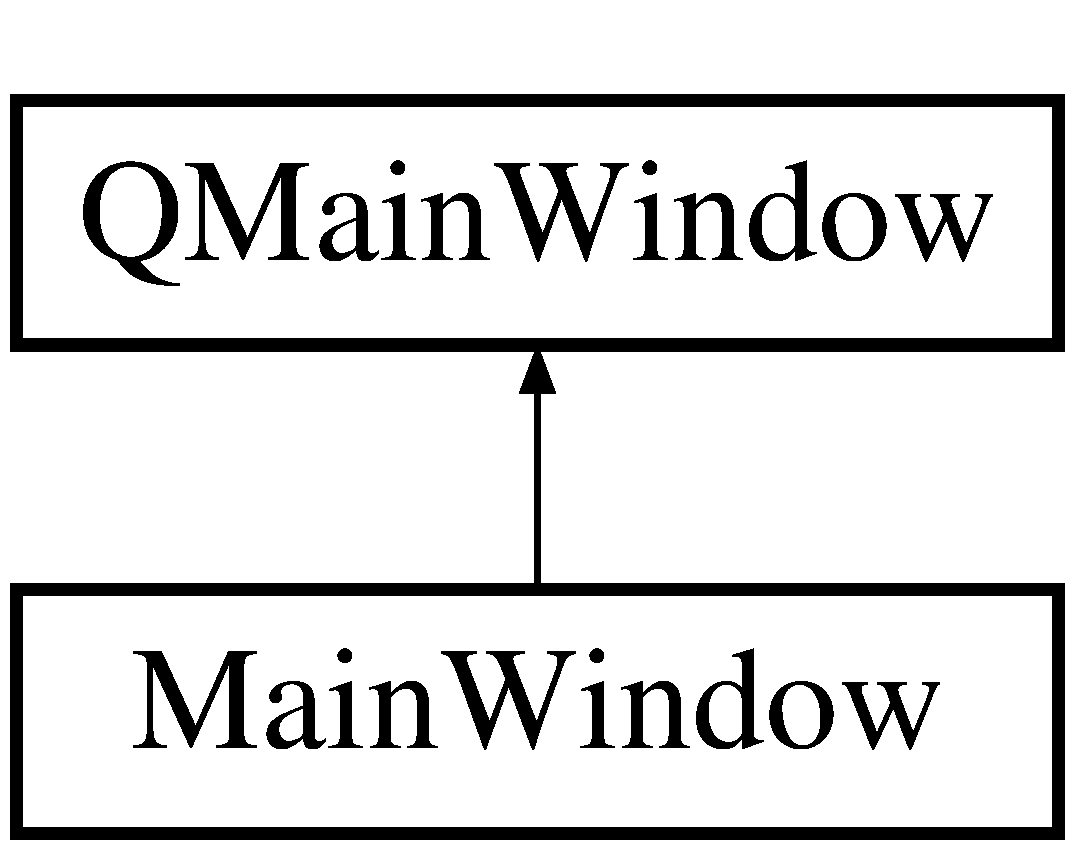
\includegraphics[height=2.000000cm]{class_main_window}
\end{center}
\end{figure}
\subsection*{Signals}
\begin{DoxyCompactItemize}
\item 
void \hyperlink{class_main_window_a6e4baaadf3320a8f9bbb42156cb78b33}{initialize\+Stadium\+Table} (\hyperlink{class_stadium_table_model}{Stadium\+Table\+Model} $\ast$stadium\+Model)
\item 
void \hyperlink{class_main_window_a53fd151cb7da7cf66320fb8cf2fb177e}{initialize\+Souvenir\+Table} (\hyperlink{class_souvenir_table_model}{Souvenir\+Table\+Model} $\ast$souvenir\+Model)
\item 
void \hyperlink{class_main_window_a36e07b34c10514f624dd59710cc844cc}{admin\+Features\+Toggled} (bool)
\item 
void \hyperlink{class_main_window_a4d5da5eb191a645b2474d1f947a51d64}{give\+DB} (\hyperlink{class_database}{Database} $\ast$db)
\item 
void \hyperlink{class_main_window_a0869694fb6c279f387d9fcb7aed8d2e9}{propagate\+Stadium\+List} (Q\+Sql\+Query)
\end{DoxyCompactItemize}
\subsection*{Public Member Functions}
\begin{DoxyCompactItemize}
\item 
\hyperlink{class_main_window_a8b244be8b7b7db1b08de2a2acb9409db}{Main\+Window} (Q\+Widget $\ast$parent=0)
\item 
\hyperlink{class_main_window_ae98d00a93bc118200eeef9f9bba1dba7}{$\sim$\+Main\+Window} ()
\end{DoxyCompactItemize}


\subsection{Detailed Description}


Definition at line 39 of file mainwindow.\+h.



\subsection{Constructor \& Destructor Documentation}
\index{Main\+Window@{Main\+Window}!Main\+Window@{Main\+Window}}
\index{Main\+Window@{Main\+Window}!Main\+Window@{Main\+Window}}
\subsubsection[{\texorpdfstring{Main\+Window(\+Q\+Widget $\ast$parent=0)}{MainWindow(QWidget *parent=0)}}]{\setlength{\rightskip}{0pt plus 5cm}Main\+Window\+::\+Main\+Window (
\begin{DoxyParamCaption}
\item[{Q\+Widget $\ast$}]{parent = {\ttfamily 0}}
\end{DoxyParamCaption}
)\hspace{0.3cm}{\ttfamily [explicit]}}\hypertarget{class_main_window_a8b244be8b7b7db1b08de2a2acb9409db}{}\label{class_main_window_a8b244be8b7b7db1b08de2a2acb9409db}


Definition at line 4 of file mainwindow.\+cpp.

\index{Main\+Window@{Main\+Window}!````~Main\+Window@{$\sim$\+Main\+Window}}
\index{````~Main\+Window@{$\sim$\+Main\+Window}!Main\+Window@{Main\+Window}}
\subsubsection[{\texorpdfstring{$\sim$\+Main\+Window()}{~MainWindow()}}]{\setlength{\rightskip}{0pt plus 5cm}Main\+Window\+::$\sim$\+Main\+Window (
\begin{DoxyParamCaption}
{}
\end{DoxyParamCaption}
)}\hypertarget{class_main_window_ae98d00a93bc118200eeef9f9bba1dba7}{}\label{class_main_window_ae98d00a93bc118200eeef9f9bba1dba7}


Definition at line 77 of file mainwindow.\+cpp.



\subsection{Member Function Documentation}
\index{Main\+Window@{Main\+Window}!admin\+Features\+Toggled@{admin\+Features\+Toggled}}
\index{admin\+Features\+Toggled@{admin\+Features\+Toggled}!Main\+Window@{Main\+Window}}
\subsubsection[{\texorpdfstring{admin\+Features\+Toggled}{adminFeaturesToggled}}]{\setlength{\rightskip}{0pt plus 5cm}void Main\+Window\+::admin\+Features\+Toggled (
\begin{DoxyParamCaption}
\item[{bool}]{}
\end{DoxyParamCaption}
)\hspace{0.3cm}{\ttfamily [signal]}}\hypertarget{class_main_window_a36e07b34c10514f624dd59710cc844cc}{}\label{class_main_window_a36e07b34c10514f624dd59710cc844cc}
\index{Main\+Window@{Main\+Window}!give\+DB@{give\+DB}}
\index{give\+DB@{give\+DB}!Main\+Window@{Main\+Window}}
\subsubsection[{\texorpdfstring{give\+DB}{giveDB}}]{\setlength{\rightskip}{0pt plus 5cm}void Main\+Window\+::give\+DB (
\begin{DoxyParamCaption}
\item[{{\bf Database} $\ast$}]{db}
\end{DoxyParamCaption}
)\hspace{0.3cm}{\ttfamily [signal]}}\hypertarget{class_main_window_a4d5da5eb191a645b2474d1f947a51d64}{}\label{class_main_window_a4d5da5eb191a645b2474d1f947a51d64}
\index{Main\+Window@{Main\+Window}!initialize\+Souvenir\+Table@{initialize\+Souvenir\+Table}}
\index{initialize\+Souvenir\+Table@{initialize\+Souvenir\+Table}!Main\+Window@{Main\+Window}}
\subsubsection[{\texorpdfstring{initialize\+Souvenir\+Table}{initializeSouvenirTable}}]{\setlength{\rightskip}{0pt plus 5cm}void Main\+Window\+::initialize\+Souvenir\+Table (
\begin{DoxyParamCaption}
\item[{{\bf Souvenir\+Table\+Model} $\ast$}]{souvenir\+Model}
\end{DoxyParamCaption}
)\hspace{0.3cm}{\ttfamily [signal]}}\hypertarget{class_main_window_a53fd151cb7da7cf66320fb8cf2fb177e}{}\label{class_main_window_a53fd151cb7da7cf66320fb8cf2fb177e}
\index{Main\+Window@{Main\+Window}!initialize\+Stadium\+Table@{initialize\+Stadium\+Table}}
\index{initialize\+Stadium\+Table@{initialize\+Stadium\+Table}!Main\+Window@{Main\+Window}}
\subsubsection[{\texorpdfstring{initialize\+Stadium\+Table}{initializeStadiumTable}}]{\setlength{\rightskip}{0pt plus 5cm}void Main\+Window\+::initialize\+Stadium\+Table (
\begin{DoxyParamCaption}
\item[{{\bf Stadium\+Table\+Model} $\ast$}]{stadium\+Model}
\end{DoxyParamCaption}
)\hspace{0.3cm}{\ttfamily [signal]}}\hypertarget{class_main_window_a6e4baaadf3320a8f9bbb42156cb78b33}{}\label{class_main_window_a6e4baaadf3320a8f9bbb42156cb78b33}
\index{Main\+Window@{Main\+Window}!propagate\+Stadium\+List@{propagate\+Stadium\+List}}
\index{propagate\+Stadium\+List@{propagate\+Stadium\+List}!Main\+Window@{Main\+Window}}
\subsubsection[{\texorpdfstring{propagate\+Stadium\+List}{propagateStadiumList}}]{\setlength{\rightskip}{0pt plus 5cm}void Main\+Window\+::propagate\+Stadium\+List (
\begin{DoxyParamCaption}
\item[{Q\+Sql\+Query}]{}
\end{DoxyParamCaption}
)\hspace{0.3cm}{\ttfamily [signal]}}\hypertarget{class_main_window_a0869694fb6c279f387d9fcb7aed8d2e9}{}\label{class_main_window_a0869694fb6c279f387d9fcb7aed8d2e9}


The documentation for this class was generated from the following files\+:\begin{DoxyCompactItemize}
\item 
src/header/\hyperlink{mainwindow_8h}{mainwindow.\+h}\item 
src/source/\hyperlink{mainwindow_8cpp}{mainwindow.\+cpp}\end{DoxyCompactItemize}

\hypertarget{struct_q_list_1_1_memory_layout}{}\section{Q\+List$<$ T $>$\+:\+:Memory\+Layout Struct Reference}
\label{struct_q_list_1_1_memory_layout}\index{Q\+List$<$ T $>$\+::\+Memory\+Layout@{Q\+List$<$ T $>$\+::\+Memory\+Layout}}


{\ttfamily \#include $<$qlist.\+h$>$}

Inheritance diagram for Q\+List$<$ T $>$\+:\+:Memory\+Layout\+:\begin{figure}[H]
\begin{center}
\leavevmode
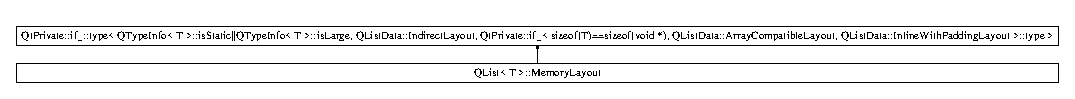
\includegraphics[height=0.886778cm]{struct_q_list_1_1_memory_layout}
\end{center}
\end{figure}


\subsection{Detailed Description}
\subsubsection*{template$<$typename T$>$\\*
struct Q\+List$<$ T $>$\+::\+Memory\+Layout}



Definition at line 116 of file qlist.\+h.



The documentation for this struct was generated from the following file\+:\begin{DoxyCompactItemize}
\item 
docs/extra-\/files/\hyperlink{qlist_8h}{qlist.\+h}\end{DoxyCompactItemize}

\hypertarget{struct_q_list_data_1_1_not_array_compatible_layout}{}\section{Q\+List\+Data\+:\+:Not\+Array\+Compatible\+Layout Struct Reference}
\label{struct_q_list_data_1_1_not_array_compatible_layout}\index{Q\+List\+Data\+::\+Not\+Array\+Compatible\+Layout@{Q\+List\+Data\+::\+Not\+Array\+Compatible\+Layout}}


{\ttfamily \#include $<$qlist.\+h$>$}

Inheritance diagram for Q\+List\+Data\+:\+:Not\+Array\+Compatible\+Layout\+:\begin{figure}[H]
\begin{center}
\leavevmode
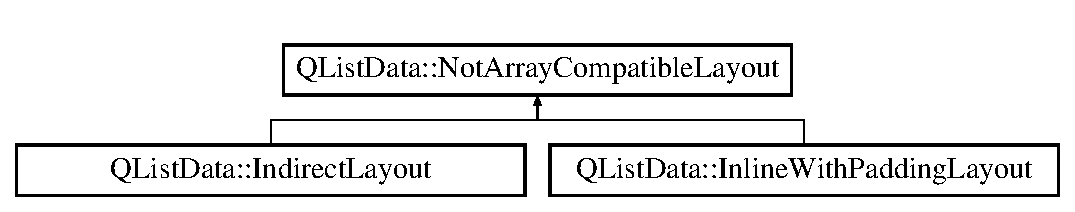
\includegraphics[height=2.000000cm]{struct_q_list_data_1_1_not_array_compatible_layout}
\end{center}
\end{figure}


\subsection{Detailed Description}


Definition at line 76 of file qlist.\+h.



The documentation for this struct was generated from the following file\+:\begin{DoxyCompactItemize}
\item 
docs/extra-\/files/\hyperlink{qlist_8h}{qlist.\+h}\end{DoxyCompactItemize}

\hypertarget{struct_q_list_data_1_1_not_indirect_layout}{}\section{Q\+List\+Data\+:\+:Not\+Indirect\+Layout Struct Reference}
\label{struct_q_list_data_1_1_not_indirect_layout}\index{Q\+List\+Data\+::\+Not\+Indirect\+Layout@{Q\+List\+Data\+::\+Not\+Indirect\+Layout}}


{\ttfamily \#include $<$qlist.\+h$>$}

Inheritance diagram for Q\+List\+Data\+:\+:Not\+Indirect\+Layout\+:\begin{figure}[H]
\begin{center}
\leavevmode
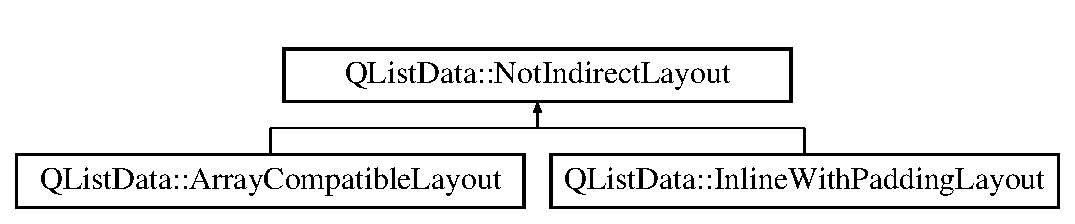
\includegraphics[height=2.000000cm]{struct_q_list_data_1_1_not_indirect_layout}
\end{center}
\end{figure}


\subsection{Detailed Description}


Definition at line 77 of file qlist.\+h.



The documentation for this struct was generated from the following file\+:\begin{DoxyCompactItemize}
\item 
docs/extra-\/files/\hyperlink{qlist_8h}{qlist.\+h}\end{DoxyCompactItemize}

\hypertarget{class_plan_trip}{}\section{Plan\+Trip Class Reference}
\label{class_plan_trip}\index{Plan\+Trip@{Plan\+Trip}}


{\ttfamily \#include $<$plantrip.\+h$>$}

Inheritance diagram for Plan\+Trip\+:\begin{figure}[H]
\begin{center}
\leavevmode
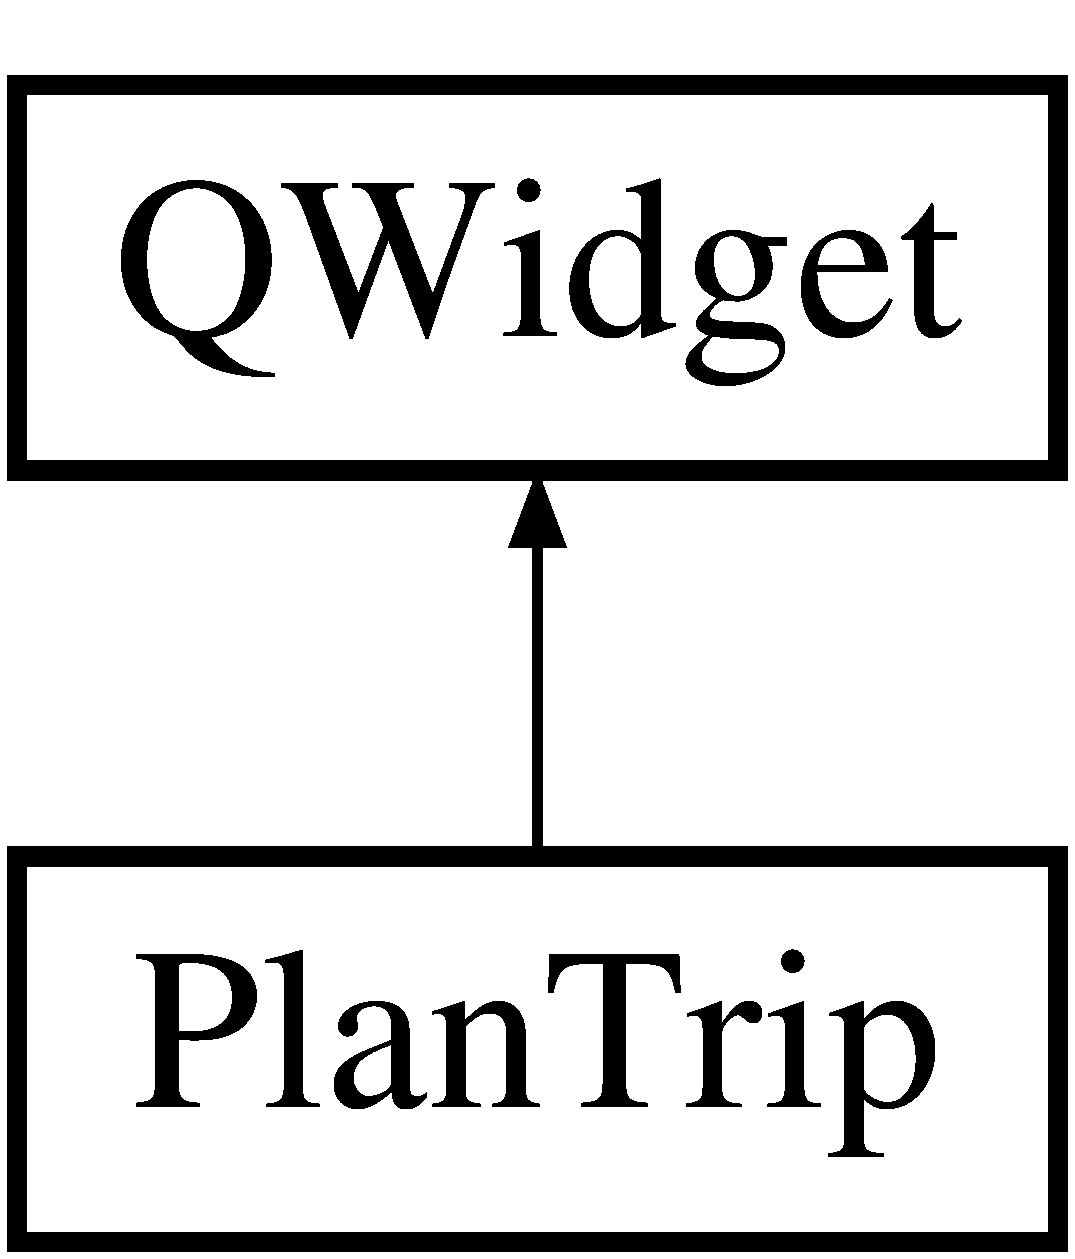
\includegraphics[height=2.000000cm]{class_plan_trip}
\end{center}
\end{figure}
\subsection*{Public Slots}
\begin{DoxyCompactItemize}
\item 
void \hyperlink{class_plan_trip_ad4e718e750e17dd0f28439a09fa65d0d}{propagate\+Stadium\+List} (Q\+Sql\+Query query)
\begin{DoxyCompactList}\small\item\em Propagate the stadiums list. \end{DoxyCompactList}\end{DoxyCompactItemize}
\subsection*{Signals}
\begin{DoxyCompactItemize}
\item 
void \hyperlink{class_plan_trip_aca48bc2b3be5f6fb459efeb3496c5466}{hide\+Next\+Button} (bool)
\begin{DoxyCompactList}\small\item\em Send a signal to hide or show the mainwindow next button. \end{DoxyCompactList}\item 
void \hyperlink{class_plan_trip_a996ab77b2600758fcaa5c98dfa77f2fd}{click\+Next} ()
\begin{DoxyCompactList}\small\item\em Send a signal to click the mainwindow next button. \end{DoxyCompactList}\item 
void \hyperlink{class_plan_trip_ac8896fbaa74477f262824c7276fbd90f}{give\+Stadium\+List} (Q\+String\+List)
\begin{DoxyCompactList}\small\item\em Send a signal with a string\+List containing the selected stadiums, in order. \end{DoxyCompactList}\item 
void \hyperlink{class_plan_trip_a8f4321d1518eaf73049755add0c9acda}{call\+Visit\+All} ()
\begin{DoxyCompactList}\small\item\em Sends a signal saying we clicked the visit all button. \end{DoxyCompactList}\item 
void \hyperlink{class_plan_trip_a11511d0b19fa50cec8e1c166b71e3843}{give\+Stadium\+List\+Visit\+All} (Q\+String\+List)
\begin{DoxyCompactList}\small\item\em Sends a signal for Visitall Stadiums for purchase cart. \end{DoxyCompactList}\item 
void \hyperlink{class_plan_trip_af5dfa60d754eb1b742fa75f8ea31ac2b}{display\+M\+ST} ()
\begin{DoxyCompactList}\small\item\em Send a signal to display the minimum spanning tree. \end{DoxyCompactList}\end{DoxyCompactItemize}
\subsection*{Public Member Functions}
\begin{DoxyCompactItemize}
\item 
\hyperlink{class_plan_trip_a560e5efbd99d17cbbccee68423ff17a5}{Plan\+Trip} (Q\+Widget $\ast$parent=0, \hyperlink{class_database}{Database} $\ast$db=0)
\item 
\hyperlink{class_plan_trip_ae6a7198bf9faca413287acd7f147543a}{$\sim$\+Plan\+Trip} ()
\end{DoxyCompactItemize}


\subsection{Detailed Description}


Definition at line 13 of file plantrip.\+h.



\subsection{Constructor \& Destructor Documentation}
\index{Plan\+Trip@{Plan\+Trip}!Plan\+Trip@{Plan\+Trip}}
\index{Plan\+Trip@{Plan\+Trip}!Plan\+Trip@{Plan\+Trip}}
\subsubsection[{\texorpdfstring{Plan\+Trip(\+Q\+Widget $\ast$parent=0, Database $\ast$db=0)}{PlanTrip(QWidget *parent=0, Database *db=0)}}]{\setlength{\rightskip}{0pt plus 5cm}Plan\+Trip\+::\+Plan\+Trip (
\begin{DoxyParamCaption}
\item[{Q\+Widget $\ast$}]{parent = {\ttfamily 0}, }
\item[{{\bf Database} $\ast$}]{db = {\ttfamily 0}}
\end{DoxyParamCaption}
)\hspace{0.3cm}{\ttfamily [explicit]}}\hypertarget{class_plan_trip_a560e5efbd99d17cbbccee68423ff17a5}{}\label{class_plan_trip_a560e5efbd99d17cbbccee68423ff17a5}


Definition at line 5 of file plantrip.\+cpp.

\index{Plan\+Trip@{Plan\+Trip}!````~Plan\+Trip@{$\sim$\+Plan\+Trip}}
\index{````~Plan\+Trip@{$\sim$\+Plan\+Trip}!Plan\+Trip@{Plan\+Trip}}
\subsubsection[{\texorpdfstring{$\sim$\+Plan\+Trip()}{~PlanTrip()}}]{\setlength{\rightskip}{0pt plus 5cm}Plan\+Trip\+::$\sim$\+Plan\+Trip (
\begin{DoxyParamCaption}
{}
\end{DoxyParamCaption}
)}\hypertarget{class_plan_trip_ae6a7198bf9faca413287acd7f147543a}{}\label{class_plan_trip_ae6a7198bf9faca413287acd7f147543a}


Definition at line 14 of file plantrip.\+cpp.



\subsection{Member Function Documentation}
\index{Plan\+Trip@{Plan\+Trip}!call\+Visit\+All@{call\+Visit\+All}}
\index{call\+Visit\+All@{call\+Visit\+All}!Plan\+Trip@{Plan\+Trip}}
\subsubsection[{\texorpdfstring{call\+Visit\+All}{callVisitAll}}]{\setlength{\rightskip}{0pt plus 5cm}void Plan\+Trip\+::call\+Visit\+All (
\begin{DoxyParamCaption}
{}
\end{DoxyParamCaption}
)\hspace{0.3cm}{\ttfamily [signal]}}\hypertarget{class_plan_trip_a8f4321d1518eaf73049755add0c9acda}{}\label{class_plan_trip_a8f4321d1518eaf73049755add0c9acda}


Sends a signal saying we clicked the visit all button. 

\index{Plan\+Trip@{Plan\+Trip}!click\+Next@{click\+Next}}
\index{click\+Next@{click\+Next}!Plan\+Trip@{Plan\+Trip}}
\subsubsection[{\texorpdfstring{click\+Next}{clickNext}}]{\setlength{\rightskip}{0pt plus 5cm}void Plan\+Trip\+::click\+Next (
\begin{DoxyParamCaption}
{}
\end{DoxyParamCaption}
)\hspace{0.3cm}{\ttfamily [signal]}}\hypertarget{class_plan_trip_a996ab77b2600758fcaa5c98dfa77f2fd}{}\label{class_plan_trip_a996ab77b2600758fcaa5c98dfa77f2fd}


Send a signal to click the mainwindow next button. 

\index{Plan\+Trip@{Plan\+Trip}!display\+M\+ST@{display\+M\+ST}}
\index{display\+M\+ST@{display\+M\+ST}!Plan\+Trip@{Plan\+Trip}}
\subsubsection[{\texorpdfstring{display\+M\+ST}{displayMST}}]{\setlength{\rightskip}{0pt plus 5cm}void Plan\+Trip\+::display\+M\+ST (
\begin{DoxyParamCaption}
{}
\end{DoxyParamCaption}
)\hspace{0.3cm}{\ttfamily [signal]}}\hypertarget{class_plan_trip_af5dfa60d754eb1b742fa75f8ea31ac2b}{}\label{class_plan_trip_af5dfa60d754eb1b742fa75f8ea31ac2b}


Send a signal to display the minimum spanning tree. 

\index{Plan\+Trip@{Plan\+Trip}!give\+Stadium\+List@{give\+Stadium\+List}}
\index{give\+Stadium\+List@{give\+Stadium\+List}!Plan\+Trip@{Plan\+Trip}}
\subsubsection[{\texorpdfstring{give\+Stadium\+List}{giveStadiumList}}]{\setlength{\rightskip}{0pt plus 5cm}void Plan\+Trip\+::give\+Stadium\+List (
\begin{DoxyParamCaption}
\item[{Q\+String\+List}]{}
\end{DoxyParamCaption}
)\hspace{0.3cm}{\ttfamily [signal]}}\hypertarget{class_plan_trip_ac8896fbaa74477f262824c7276fbd90f}{}\label{class_plan_trip_ac8896fbaa74477f262824c7276fbd90f}


Send a signal with a string\+List containing the selected stadiums, in order. 

\index{Plan\+Trip@{Plan\+Trip}!give\+Stadium\+List\+Visit\+All@{give\+Stadium\+List\+Visit\+All}}
\index{give\+Stadium\+List\+Visit\+All@{give\+Stadium\+List\+Visit\+All}!Plan\+Trip@{Plan\+Trip}}
\subsubsection[{\texorpdfstring{give\+Stadium\+List\+Visit\+All}{giveStadiumListVisitAll}}]{\setlength{\rightskip}{0pt plus 5cm}void Plan\+Trip\+::give\+Stadium\+List\+Visit\+All (
\begin{DoxyParamCaption}
\item[{Q\+String\+List}]{}
\end{DoxyParamCaption}
)\hspace{0.3cm}{\ttfamily [signal]}}\hypertarget{class_plan_trip_a11511d0b19fa50cec8e1c166b71e3843}{}\label{class_plan_trip_a11511d0b19fa50cec8e1c166b71e3843}


Sends a signal for Visitall Stadiums for purchase cart. 

\index{Plan\+Trip@{Plan\+Trip}!hide\+Next\+Button@{hide\+Next\+Button}}
\index{hide\+Next\+Button@{hide\+Next\+Button}!Plan\+Trip@{Plan\+Trip}}
\subsubsection[{\texorpdfstring{hide\+Next\+Button}{hideNextButton}}]{\setlength{\rightskip}{0pt plus 5cm}void Plan\+Trip\+::hide\+Next\+Button (
\begin{DoxyParamCaption}
\item[{bool}]{}
\end{DoxyParamCaption}
)\hspace{0.3cm}{\ttfamily [signal]}}\hypertarget{class_plan_trip_aca48bc2b3be5f6fb459efeb3496c5466}{}\label{class_plan_trip_aca48bc2b3be5f6fb459efeb3496c5466}


Send a signal to hide or show the mainwindow next button. 

\index{Plan\+Trip@{Plan\+Trip}!propagate\+Stadium\+List@{propagate\+Stadium\+List}}
\index{propagate\+Stadium\+List@{propagate\+Stadium\+List}!Plan\+Trip@{Plan\+Trip}}
\subsubsection[{\texorpdfstring{propagate\+Stadium\+List}{propagateStadiumList}}]{\setlength{\rightskip}{0pt plus 5cm}void Plan\+Trip\+::propagate\+Stadium\+List (
\begin{DoxyParamCaption}
\item[{Q\+Sql\+Query}]{query}
\end{DoxyParamCaption}
)\hspace{0.3cm}{\ttfamily [slot]}}\hypertarget{class_plan_trip_ad4e718e750e17dd0f28439a09fa65d0d}{}\label{class_plan_trip_ad4e718e750e17dd0f28439a09fa65d0d}


Propagate the stadiums list. 

\hyperlink{class_plan_trip_ad4e718e750e17dd0f28439a09fa65d0d}{Plan\+Trip\+::propagate\+Stadium\+List} Use a S\+QL query object to propagate the stadium list with stadium names.


\begin{DoxyParams}{Parameters}
{\em query} & \\
\hline
\end{DoxyParams}


Definition at line 24 of file plantrip.\+cpp.



The documentation for this class was generated from the following files\+:\begin{DoxyCompactItemize}
\item 
src/header/\hyperlink{plantrip_8h}{plantrip.\+h}\item 
src/source/\hyperlink{plantrip_8cpp}{plantrip.\+cpp}\end{DoxyCompactItemize}

\hypertarget{struct_purchase_window_1_1purchase_info}{}\section{Purchase\+Window\+:\+:purchase\+Info Struct Reference}
\label{struct_purchase_window_1_1purchase_info}\index{Purchase\+Window\+::purchase\+Info@{Purchase\+Window\+::purchase\+Info}}


{\ttfamily \#include $<$purchasewindow.\+h$>$}

\subsection*{Public Attributes}
\begin{DoxyCompactItemize}
\item 
Q\+String \hyperlink{struct_purchase_window_1_1purchase_info_a36aa0c95851cabe4198c52a415936830}{stadium\+Name}
\item 
Q\+String \hyperlink{struct_purchase_window_1_1purchase_info_a49fb075ed3df267b7991658c08e4f0fe}{item\+Name}
\item 
double \hyperlink{struct_purchase_window_1_1purchase_info_a411ad453985ea6da851b601b2224e169}{item\+Price}
\item 
int \hyperlink{struct_purchase_window_1_1purchase_info_a2d9677095f95648ad805d8abafeae063}{quantity}
\end{DoxyCompactItemize}


\subsection{Detailed Description}


Definition at line 20 of file purchasewindow.\+h.



\subsection{Member Data Documentation}
\index{Purchase\+Window\+::purchase\+Info@{Purchase\+Window\+::purchase\+Info}!item\+Name@{item\+Name}}
\index{item\+Name@{item\+Name}!Purchase\+Window\+::purchase\+Info@{Purchase\+Window\+::purchase\+Info}}
\subsubsection[{\texorpdfstring{item\+Name}{itemName}}]{\setlength{\rightskip}{0pt plus 5cm}Q\+String Purchase\+Window\+::purchase\+Info\+::item\+Name}\hypertarget{struct_purchase_window_1_1purchase_info_a49fb075ed3df267b7991658c08e4f0fe}{}\label{struct_purchase_window_1_1purchase_info_a49fb075ed3df267b7991658c08e4f0fe}


Definition at line 22 of file purchasewindow.\+h.

\index{Purchase\+Window\+::purchase\+Info@{Purchase\+Window\+::purchase\+Info}!item\+Price@{item\+Price}}
\index{item\+Price@{item\+Price}!Purchase\+Window\+::purchase\+Info@{Purchase\+Window\+::purchase\+Info}}
\subsubsection[{\texorpdfstring{item\+Price}{itemPrice}}]{\setlength{\rightskip}{0pt plus 5cm}double Purchase\+Window\+::purchase\+Info\+::item\+Price}\hypertarget{struct_purchase_window_1_1purchase_info_a411ad453985ea6da851b601b2224e169}{}\label{struct_purchase_window_1_1purchase_info_a411ad453985ea6da851b601b2224e169}


Definition at line 23 of file purchasewindow.\+h.

\index{Purchase\+Window\+::purchase\+Info@{Purchase\+Window\+::purchase\+Info}!quantity@{quantity}}
\index{quantity@{quantity}!Purchase\+Window\+::purchase\+Info@{Purchase\+Window\+::purchase\+Info}}
\subsubsection[{\texorpdfstring{quantity}{quantity}}]{\setlength{\rightskip}{0pt plus 5cm}int Purchase\+Window\+::purchase\+Info\+::quantity}\hypertarget{struct_purchase_window_1_1purchase_info_a2d9677095f95648ad805d8abafeae063}{}\label{struct_purchase_window_1_1purchase_info_a2d9677095f95648ad805d8abafeae063}


Definition at line 24 of file purchasewindow.\+h.

\index{Purchase\+Window\+::purchase\+Info@{Purchase\+Window\+::purchase\+Info}!stadium\+Name@{stadium\+Name}}
\index{stadium\+Name@{stadium\+Name}!Purchase\+Window\+::purchase\+Info@{Purchase\+Window\+::purchase\+Info}}
\subsubsection[{\texorpdfstring{stadium\+Name}{stadiumName}}]{\setlength{\rightskip}{0pt plus 5cm}Q\+String Purchase\+Window\+::purchase\+Info\+::stadium\+Name}\hypertarget{struct_purchase_window_1_1purchase_info_a36aa0c95851cabe4198c52a415936830}{}\label{struct_purchase_window_1_1purchase_info_a36aa0c95851cabe4198c52a415936830}


Definition at line 21 of file purchasewindow.\+h.



The documentation for this struct was generated from the following file\+:\begin{DoxyCompactItemize}
\item 
src/header/\hyperlink{purchasewindow_8h}{purchasewindow.\+h}\end{DoxyCompactItemize}

\hypertarget{class_purchase_window}{}\section{Purchase\+Window Class Reference}
\label{class_purchase_window}\index{Purchase\+Window@{Purchase\+Window}}


{\ttfamily \#include $<$purchasewindow.\+h$>$}

Inheritance diagram for Purchase\+Window\+:\begin{figure}[H]
\begin{center}
\leavevmode
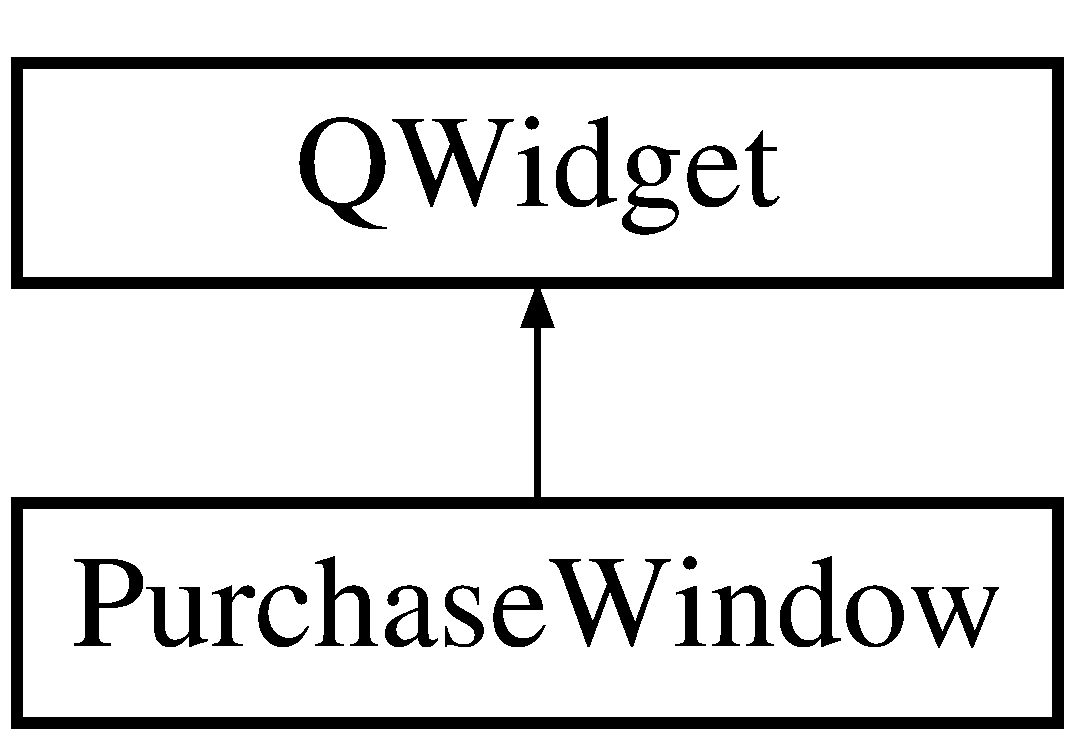
\includegraphics[height=2.000000cm]{class_purchase_window}
\end{center}
\end{figure}
\subsection*{Classes}
\begin{DoxyCompactItemize}
\item 
struct \hyperlink{struct_purchase_window_1_1purchase_info}{purchase\+Info}
\end{DoxyCompactItemize}
\subsection*{Public Slots}
\begin{DoxyCompactItemize}
\item 
void \hyperlink{class_purchase_window_a6f1bfcc93c4cb61b56b1707671e13ba8}{propagate\+Stadium\+List} (Q\+String\+List stadiums)
\begin{DoxyCompactList}\small\item\em \hyperlink{class_purchase_window_a6f1bfcc93c4cb61b56b1707671e13ba8}{Purchase\+Window\+::propagate\+Stadium\+List} Propagate the combo\+Box with the list of selected stadiums to visit. \end{DoxyCompactList}\end{DoxyCompactItemize}
\subsection*{Public Member Functions}
\begin{DoxyCompactItemize}
\item 
\hyperlink{class_purchase_window_a6aa4014cd9a1eb8e4b9372d7161ce990}{Purchase\+Window} (Q\+Widget $\ast$parent=0, \hyperlink{class_database}{Database} $\ast$db=0)
\item 
\hyperlink{class_purchase_window_afb8082268943606816568f5bf40a1f6f}{$\sim$\+Purchase\+Window} ()
\item 
\hyperlink{class_q_list}{Q\+List}$<$ \hyperlink{struct_purchase_window_1_1purchase_info}{purchase\+Info} $>$ \hyperlink{class_purchase_window_a088a4f0910f7ef9503b0452523b492ab}{get\+Purchases} ()
\begin{DoxyCompactList}\small\item\em \hyperlink{class_purchase_window_a088a4f0910f7ef9503b0452523b492ab}{Purchase\+Window\+::get\+Purchases} Retrieve a list of \hyperlink{struct_purchase_window_1_1purchase_info}{purchase\+Info} structs containing all of the data in the souvenir purchase list (cart). contains\+: \end{DoxyCompactList}\end{DoxyCompactItemize}


\subsection{Detailed Description}


Definition at line 12 of file purchasewindow.\+h.



\subsection{Constructor \& Destructor Documentation}
\index{Purchase\+Window@{Purchase\+Window}!Purchase\+Window@{Purchase\+Window}}
\index{Purchase\+Window@{Purchase\+Window}!Purchase\+Window@{Purchase\+Window}}
\subsubsection[{\texorpdfstring{Purchase\+Window(\+Q\+Widget $\ast$parent=0, Database $\ast$db=0)}{PurchaseWindow(QWidget *parent=0, Database *db=0)}}]{\setlength{\rightskip}{0pt plus 5cm}Purchase\+Window\+::\+Purchase\+Window (
\begin{DoxyParamCaption}
\item[{Q\+Widget $\ast$}]{parent = {\ttfamily 0}, }
\item[{{\bf Database} $\ast$}]{db = {\ttfamily 0}}
\end{DoxyParamCaption}
)\hspace{0.3cm}{\ttfamily [explicit]}}\hypertarget{class_purchase_window_a6aa4014cd9a1eb8e4b9372d7161ce990}{}\label{class_purchase_window_a6aa4014cd9a1eb8e4b9372d7161ce990}


Definition at line 5 of file purchasewindow.\+cpp.

\index{Purchase\+Window@{Purchase\+Window}!````~Purchase\+Window@{$\sim$\+Purchase\+Window}}
\index{````~Purchase\+Window@{$\sim$\+Purchase\+Window}!Purchase\+Window@{Purchase\+Window}}
\subsubsection[{\texorpdfstring{$\sim$\+Purchase\+Window()}{~PurchaseWindow()}}]{\setlength{\rightskip}{0pt plus 5cm}Purchase\+Window\+::$\sim$\+Purchase\+Window (
\begin{DoxyParamCaption}
{}
\end{DoxyParamCaption}
)}\hypertarget{class_purchase_window_afb8082268943606816568f5bf40a1f6f}{}\label{class_purchase_window_afb8082268943606816568f5bf40a1f6f}


Definition at line 57 of file purchasewindow.\+cpp.



\subsection{Member Function Documentation}
\index{Purchase\+Window@{Purchase\+Window}!get\+Purchases@{get\+Purchases}}
\index{get\+Purchases@{get\+Purchases}!Purchase\+Window@{Purchase\+Window}}
\subsubsection[{\texorpdfstring{get\+Purchases()}{getPurchases()}}]{\setlength{\rightskip}{0pt plus 5cm}{\bf Q\+List}$<$ {\bf Purchase\+Window\+::purchase\+Info} $>$ Purchase\+Window\+::get\+Purchases (
\begin{DoxyParamCaption}
{}
\end{DoxyParamCaption}
)}\hypertarget{class_purchase_window_a088a4f0910f7ef9503b0452523b492ab}{}\label{class_purchase_window_a088a4f0910f7ef9503b0452523b492ab}


\hyperlink{class_purchase_window_a088a4f0910f7ef9503b0452523b492ab}{Purchase\+Window\+::get\+Purchases} Retrieve a list of \hyperlink{struct_purchase_window_1_1purchase_info}{purchase\+Info} structs containing all of the data in the souvenir purchase list (cart). contains\+: 


\begin{DoxyItemize}
\item stadium name
\item item name
\item item price
\item item quantity
\end{DoxyItemize}

\begin{DoxyReturn}{Returns}
purchases a list of \hyperlink{struct_purchase_window_1_1purchase_info}{purchase\+Info} structs 
\end{DoxyReturn}


Definition at line 74 of file purchasewindow.\+cpp.

\index{Purchase\+Window@{Purchase\+Window}!propagate\+Stadium\+List@{propagate\+Stadium\+List}}
\index{propagate\+Stadium\+List@{propagate\+Stadium\+List}!Purchase\+Window@{Purchase\+Window}}
\subsubsection[{\texorpdfstring{propagate\+Stadium\+List}{propagateStadiumList}}]{\setlength{\rightskip}{0pt plus 5cm}void Purchase\+Window\+::propagate\+Stadium\+List (
\begin{DoxyParamCaption}
\item[{Q\+String\+List}]{stadiums}
\end{DoxyParamCaption}
)\hspace{0.3cm}{\ttfamily [slot]}}\hypertarget{class_purchase_window_a6f1bfcc93c4cb61b56b1707671e13ba8}{}\label{class_purchase_window_a6f1bfcc93c4cb61b56b1707671e13ba8}


\hyperlink{class_purchase_window_a6f1bfcc93c4cb61b56b1707671e13ba8}{Purchase\+Window\+::propagate\+Stadium\+List} Propagate the combo\+Box with the list of selected stadiums to visit. 


\begin{DoxyParams}{Parameters}
{\em stadiums} & Q\+String\+List of stadium names \\
\hline
\end{DoxyParams}


Definition at line 121 of file purchasewindow.\+cpp.



The documentation for this class was generated from the following files\+:\begin{DoxyCompactItemize}
\item 
src/header/\hyperlink{purchasewindow_8h}{purchasewindow.\+h}\item 
src/source/\hyperlink{purchasewindow_8cpp}{purchasewindow.\+cpp}\end{DoxyCompactItemize}

\hypertarget{class_q_list}{}\section{Q\+List$<$ T $>$ Class Template Reference}
\label{class_q_list}\index{Q\+List$<$ T $>$@{Q\+List$<$ T $>$}}


The \hyperlink{class_q_list}{Q\+List} class is a template class that provides lists.  




{\ttfamily \#include $<$qlist.\+h$>$}

Inheritance diagram for Q\+List$<$ T $>$\+:\begin{figure}[H]
\begin{center}
\leavevmode
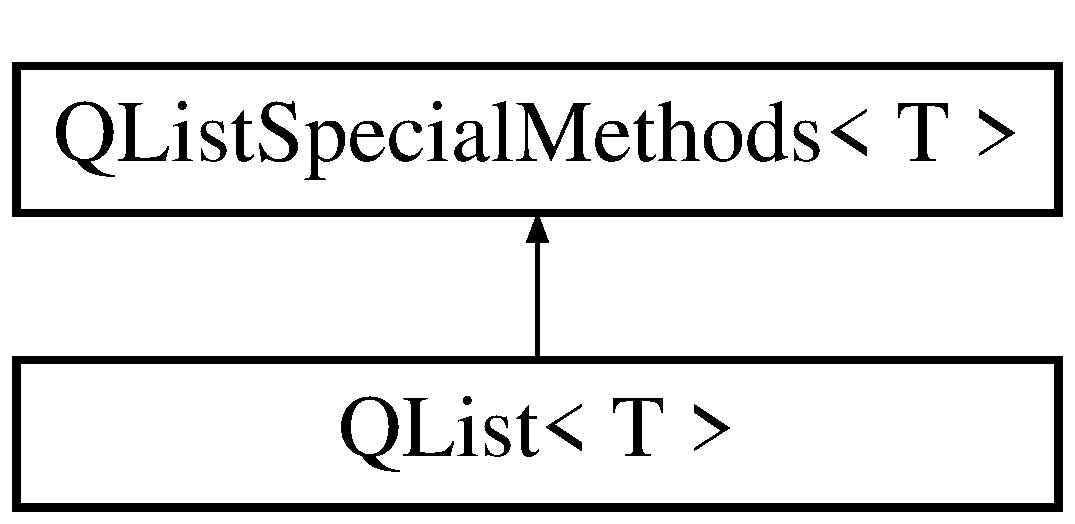
\includegraphics[height=2.000000cm]{class_q_list}
\end{center}
\end{figure}
\subsection*{Classes}
\begin{DoxyCompactItemize}
\item 
class \hyperlink{class_q_list_1_1const__iterator}{const\+\_\+iterator}
\begin{DoxyCompactList}\small\item\em The \hyperlink{class_q_list_1_1const__iterator}{Q\+List\+::const\+\_\+iterator} class provides an S\+T\+L-\/style const iterator for \hyperlink{class_q_list}{Q\+List} and Q\+Queue. \end{DoxyCompactList}\item 
class \hyperlink{class_q_list_1_1iterator}{iterator}
\begin{DoxyCompactList}\small\item\em The \hyperlink{class_q_list_1_1iterator}{Q\+List\+::iterator} class provides an S\+T\+L-\/style non-\/const iterator for \hyperlink{class_q_list}{Q\+List} and Q\+Queue. \end{DoxyCompactList}\item 
struct \hyperlink{struct_q_list_1_1_memory_layout}{Memory\+Layout}
\end{DoxyCompactItemize}
\subsection*{Public Types}
\begin{DoxyCompactItemize}
\item 
typedef \hyperlink{class_q_list_1_1iterator}{iterator} \hyperlink{class_q_list_acfbe3160851f25b0daeec4c7b0439f35}{Iterator}
\item 
typedef \hyperlink{class_q_list_1_1const__iterator}{const\+\_\+iterator} \hyperlink{class_q_list_a2bac7028ad973eb7ff10b2bb1fc58305}{Const\+Iterator}
\item 
typedef int \hyperlink{class_q_list_a5b78b75651f6641fe9339b050508aa6f}{size\+\_\+type}
\item 
typedef T \hyperlink{class_q_list_a5c685421300b8a855730c9b06ff43605}{value\+\_\+type}
\item 
typedef \hyperlink{class_q_list_a5c685421300b8a855730c9b06ff43605}{value\+\_\+type} $\ast$ \hyperlink{class_q_list_ad81e368aee3084fe5ddc056fa649a4ac}{pointer}
\item 
typedef const \hyperlink{class_q_list_a5c685421300b8a855730c9b06ff43605}{value\+\_\+type} $\ast$ \hyperlink{class_q_list_ac2d1086a1098740e3ee2ed66e4f63f7b}{const\+\_\+pointer}
\item 
typedef \hyperlink{class_q_list_a5c685421300b8a855730c9b06ff43605}{value\+\_\+type} \& \hyperlink{class_q_list_adc9961317867d5844c90efac09c09bfb}{reference}
\item 
typedef const \hyperlink{class_q_list_a5c685421300b8a855730c9b06ff43605}{value\+\_\+type} \& \hyperlink{class_q_list_ae8717226a5e2af5b53d3e22d4b1654aa}{const\+\_\+reference}
\item 
typedef qptrdiff \hyperlink{class_q_list_a253a81bf62c0d83e0f5e8abc61ac87f9}{difference\+\_\+type}
\end{DoxyCompactItemize}
\subsection*{Public Member Functions}
\begin{DoxyCompactItemize}
\item 
\hyperlink{class_q_list_a74043360170a66953054a21e9661e274}{Q\+List} () Q\+\_\+\+D\+E\+C\+L\+\_\+\+N\+O\+T\+H\+R\+OW
\item 
\hyperlink{class_q_list_a43794b89e15c6c36bd2ae2054c4f8de2}{Q\+List} (const \hyperlink{class_q_list}{Q\+List}$<$ T $>$ \&l)
\item 
\hyperlink{class_q_list_a0c359563cd4585ffeab2d71e7f523811}{$\sim$\+Q\+List} ()
\item 
\hyperlink{class_q_list}{Q\+List}$<$ T $>$ \& \hyperlink{class_q_list_af210d61c252a7f0124854a9fea8fc23d}{operator=} (const \hyperlink{class_q_list}{Q\+List}$<$ T $>$ \&l)
\item 
void \hyperlink{class_q_list_a0db2f46bd41dd9ce5553f0be73825eb6}{swap} (\hyperlink{class_q_list}{Q\+List}$<$ T $>$ \&other)
\item 
bool \hyperlink{class_q_list_a5de7da6896f7bd2a446dbdaab6466c0f}{operator==} (const \hyperlink{class_q_list}{Q\+List}$<$ T $>$ \&l) const 
\item 
bool \hyperlink{class_q_list_ad3d2c51aa92fbff38a7dfe5ad8e6b1e7}{operator!=} (const \hyperlink{class_q_list}{Q\+List}$<$ T $>$ \&l) const 
\item 
int \hyperlink{class_q_list_a2ee18cf0bec5e1d0951a1ca1ccfb93fe}{size} () const 
\item 
void \hyperlink{class_q_list_a522859faa6db19022d44dd799078c199}{detach} ()
\item 
void \hyperlink{class_q_list_af112ea5d3c4200a720e248dffc39c4cc}{detach\+Shared} ()
\item 
bool \hyperlink{class_q_list_aa130852a9913d0d152900acbf142f81c}{is\+Detached} () const 
\item 
bool \hyperlink{class_q_list_ae89d314b75b59e294eed8597202ca74e}{is\+Shared\+With} (const \hyperlink{class_q_list}{Q\+List}$<$ T $>$ \&other) const 
\item 
bool \hyperlink{class_q_list_a7425e13d514dd7adc3cf210679eea5c3}{is\+Empty} () const 
\item 
void \hyperlink{class_q_list_a19c0e32852df02f13bd2a4dd3d637f04}{clear} ()
\item 
const T \& \hyperlink{class_q_list_a0cc68a58145ae69d679da558f4d5e849}{at} (int i) const 
\item 
const T \& \hyperlink{class_q_list_ac143057ba0fa5934e704e5ff638339d4}{operator\mbox{[}$\,$\mbox{]}} (int i) const 
\item 
T \& \hyperlink{class_q_list_aaa62d7f41e6fc05dff4da8dba575bfe6}{operator\mbox{[}$\,$\mbox{]}} (int i)
\item 
void \hyperlink{class_q_list_aedf0849585d0ba83a3ca3cce25fcddb1}{reserve} (int \hyperlink{class_q_list_a2ee18cf0bec5e1d0951a1ca1ccfb93fe}{size})
\item 
void \hyperlink{class_q_list_a3a1e18c5fb9cc04324825a46540638c5}{append} (const T \&t)
\item 
void \hyperlink{class_q_list_a16e557469f7a3562adb43ebbd46354db}{append} (const \hyperlink{class_q_list}{Q\+List}$<$ T $>$ \&t)
\item 
void \hyperlink{class_q_list_a3d6003bfe5d2e7495df9dae2902743d0}{prepend} (const T \&t)
\item 
void \hyperlink{class_q_list_a2ae4b66fdb5875c4c55eb903fa5ca25b}{insert} (int i, const T \&t)
\item 
void \hyperlink{class_q_list_ab39c49b508cf66371cc536c2bc3fb544}{replace} (int i, const T \&t)
\item 
void \hyperlink{class_q_list_a318a24dd49568516ad82cc341fe1aada}{remove\+At} (int i)
\item 
int \hyperlink{class_q_list_af882739967540dbf2810411f997039de}{remove\+All} (const T \&t)
\item 
bool \hyperlink{class_q_list_a4d25954344152f81e20ec6171f1bbcbd}{remove\+One} (const T \&t)
\item 
T \hyperlink{class_q_list_a078f9ab0404fcfb8fcc0ee1b7c6699c4}{take\+At} (int i)
\item 
T \hyperlink{class_q_list_a8059621f8145f7b79278f619c1bb0e47}{take\+First} ()
\item 
T \hyperlink{class_q_list_a410757ac0ab9febcda1541fa43adb98c}{take\+Last} ()
\item 
void \hyperlink{class_q_list_a19a4be38371f5a6b340b246a247b1f67}{move} (int from, int to)
\item 
void \hyperlink{class_q_list_ac9689c368581be3ad0ae047292c007fa}{swap} (int i, int j)
\item 
int \hyperlink{class_q_list_a1fa87bbf834812e0f400d8c14ab35b8a}{index\+Of} (const T \&t, int from=0) const 
\item 
int \hyperlink{class_q_list_aa0b792f98f9cf740bb6a8774572eac18}{last\+Index\+Of} (const T \&t, int from=-\/1) const 
\item 
bool \hyperlink{class_q_list_aedb4de9a920c63b531d2064bf0bee652}{contains} (const T \&t) const 
\item 
int \hyperlink{class_q_list_a0d021cc6668a845a26097dc9d36e8c2f}{count} (const T \&t) const 
\item 
\hyperlink{class_q_list_1_1iterator}{iterator} \hyperlink{class_q_list_a06847e57431af245c937c8cfe1c14761}{begin} ()
\item 
\hyperlink{class_q_list_1_1const__iterator}{const\+\_\+iterator} \hyperlink{class_q_list_a9bbf2e9781ec8f486f35d680c100c8bd}{begin} () const 
\item 
\hyperlink{class_q_list_1_1const__iterator}{const\+\_\+iterator} \hyperlink{class_q_list_a3777e78981166825439ff10be6475152}{cbegin} () const 
\item 
\hyperlink{class_q_list_1_1const__iterator}{const\+\_\+iterator} \hyperlink{class_q_list_a8f6d53fe01e1c2aaea0a446580f99cdb}{const\+Begin} () const 
\item 
\hyperlink{class_q_list_1_1iterator}{iterator} \hyperlink{class_q_list_a5695ddeb676cedece5b061eba08c1d0c}{end} ()
\item 
\hyperlink{class_q_list_1_1const__iterator}{const\+\_\+iterator} \hyperlink{class_q_list_a132567f83a4c5f5a2a7073c3fe200c28}{end} () const 
\item 
\hyperlink{class_q_list_1_1const__iterator}{const\+\_\+iterator} \hyperlink{class_q_list_a37f3b118d722e64fb834121fa3858fc4}{cend} () const 
\item 
\hyperlink{class_q_list_1_1const__iterator}{const\+\_\+iterator} \hyperlink{class_q_list_a66e34d5df478dda9190b9b075317690d}{const\+End} () const 
\item 
\hyperlink{class_q_list_1_1iterator}{iterator} \hyperlink{class_q_list_ae8308037e361e7e9112987ed41beefb6}{insert} (\hyperlink{class_q_list_1_1iterator}{iterator} before, const T \&t)
\item 
\hyperlink{class_q_list_1_1iterator}{iterator} \hyperlink{class_q_list_abe1d81b038b41b873794dab10bbb4ffd}{erase} (\hyperlink{class_q_list_1_1iterator}{iterator} pos)
\item 
\hyperlink{class_q_list_1_1iterator}{iterator} \hyperlink{class_q_list_a6873182c98006cfc7d4bd4637f2122b1}{erase} (\hyperlink{class_q_list_1_1iterator}{iterator} \hyperlink{class_q_list_a0d91b8dcfdf240b85c2349f339021cfa}{first}, \hyperlink{class_q_list_1_1iterator}{iterator} \hyperlink{class_q_list_a0e12e5e4af39fe20f860fe88a4fbc258}{last})
\item 
int \hyperlink{class_q_list_a94d3d2a8770163005f619c4fc6715b58}{count} () const 
\item 
int \hyperlink{class_q_list_ac1755c03849804156e624efcd6562874}{length} () const 
\item 
T \& \hyperlink{class_q_list_a0d91b8dcfdf240b85c2349f339021cfa}{first} ()
\item 
const T \& \hyperlink{class_q_list_ae6dd7daa61bc35d4087d86ed48a94483}{first} () const 
\item 
T \& \hyperlink{class_q_list_a0e12e5e4af39fe20f860fe88a4fbc258}{last} ()
\item 
const T \& \hyperlink{class_q_list_aea03869b849a94805b4f32efcfb91f6c}{last} () const 
\item 
void \hyperlink{class_q_list_a46dbbac39b9f24f1d4432a40dfea58e7}{remove\+First} ()
\item 
void \hyperlink{class_q_list_a755672d6b82fc61e949a5b803b531855}{remove\+Last} ()
\item 
bool \hyperlink{class_q_list_a6f3ab95623c1be43d05579604e9725c3}{starts\+With} (const T \&t) const 
\item 
bool \hyperlink{class_q_list_a56fc27955aa88be311fcc586b90ec1b7}{ends\+With} (const T \&t) const 
\item 
\hyperlink{class_q_list}{Q\+List}$<$ T $>$ \hyperlink{class_q_list_a92da113812831b97bac90aec3e49ec4f}{mid} (int pos, int \hyperlink{class_q_list_ac1755c03849804156e624efcd6562874}{length}=-\/1) const 
\item 
T \hyperlink{class_q_list_a3b4873989858726d6c67ee0c2cef23f9}{value} (int i) const 
\item 
T \hyperlink{class_q_list_a069f4168424cb4ea5fa737845e0344c5}{value} (int i, const T \&default\+Value) const 
\item 
void \hyperlink{class_q_list_a23747ae8cb19b7e4bf24de944aa97bf2}{push\+\_\+back} (const T \&t)
\item 
void \hyperlink{class_q_list_aa0ffa16b4f92679d5d8f96fbaf872b0a}{push\+\_\+front} (const T \&t)
\item 
T \& \hyperlink{class_q_list_abfdbbac7bf0f4bb038a4970e526a16dd}{front} ()
\item 
const T \& \hyperlink{class_q_list_a4e8454fbc329f687de1a4f4521fc6014}{front} () const 
\item 
T \& \hyperlink{class_q_list_a7083f8e5508d1e9d3fcd0e08e2e5856b}{back} ()
\item 
const T \& \hyperlink{class_q_list_ad594bd054a766853a55ab37dede212fb}{back} () const 
\item 
void \hyperlink{class_q_list_a962412c448917350122d257ffe589f72}{pop\+\_\+front} ()
\item 
void \hyperlink{class_q_list_adb1888f063a883ecc656a1daf0347a79}{pop\+\_\+back} ()
\item 
bool \hyperlink{class_q_list_af93da7b266824a11caae7cd3e5900d30}{empty} () const 
\item 
\hyperlink{class_q_list}{Q\+List}$<$ T $>$ \& \hyperlink{class_q_list_a6f36674c5ad943e3a23cfc73c0a2fee1}{operator+=} (const \hyperlink{class_q_list}{Q\+List}$<$ T $>$ \&l)
\item 
\hyperlink{class_q_list}{Q\+List}$<$ T $>$ \hyperlink{class_q_list_a7ed66a2541edf55b0ea33778778ee6c0}{operator+} (const \hyperlink{class_q_list}{Q\+List}$<$ T $>$ \&l) const 
\item 
\hyperlink{class_q_list}{Q\+List}$<$ T $>$ \& \hyperlink{class_q_list_a63856d5ed93fdf5e9f6c188415d81839}{operator+=} (const T \&t)
\item 
\hyperlink{class_q_list}{Q\+List}$<$ T $>$ \& \hyperlink{class_q_list_ac2346b83b0fce8b70836bd7a660ec346}{operator$<$$<$} (const T \&t)
\item 
\hyperlink{class_q_list}{Q\+List}$<$ T $>$ \& \hyperlink{class_q_list_a902fc01867da3047603546e10bb102e6}{operator$<$$<$} (const \hyperlink{class_q_list}{Q\+List}$<$ T $>$ \&l)
\item 
\hyperlink{class_q_vector}{Q\+Vector}$<$ T $>$ \hyperlink{class_q_list_a2cd704f6f4c066e501e170fd8c11cf28}{to\+Vector} () const 
\item 
\hyperlink{class_q_set}{Q\+Set}$<$ T $>$ \hyperlink{class_q_list_af534f77fa45d1f5c70bae4fcb1341803}{to\+Set} () const 
\item 
std\+::list$<$ T $>$ \hyperlink{class_q_list_a4da73cbb34b8ace233ec93eacc6ddb79}{to\+Std\+List} () const 
\end{DoxyCompactItemize}
\subsection*{Static Public Member Functions}
\begin{DoxyCompactItemize}
\item 
static \hyperlink{class_q_list}{Q\+List}$<$ T $>$ \hyperlink{class_q_list_ac9f7e64d962222b0660e51adbd128ef7}{from\+Vector} (const \hyperlink{class_q_vector}{Q\+Vector}$<$ T $>$ \&vector)
\item 
static \hyperlink{class_q_list}{Q\+List}$<$ T $>$ \hyperlink{class_q_list_a11d8c4df34e11f1f5539ea37f3d2130b}{from\+Set} (const \hyperlink{class_q_set}{Q\+Set}$<$ T $>$ \&set)
\item 
static \hyperlink{class_q_list}{Q\+List}$<$ T $>$ \hyperlink{class_q_list_af0810b38261117b3616803519d825c9c}{from\+Std\+List} (const std\+::list$<$ T $>$ \&list)
\end{DoxyCompactItemize}
\subsection*{Friends}
\begin{DoxyCompactItemize}
\item 
class \hyperlink{class_q_list_a67171474c4da6cc8efe0c7fafefd2b2d}{iterator}
\item 
class \hyperlink{class_q_list_ac220ce1c155db1ac44146c12d178056f}{const\+\_\+iterator}
\end{DoxyCompactItemize}
\subsection*{Related Functions}
(Note that these are not member functions.) \begin{DoxyCompactItemize}
\item 
Q\+Data\+Stream \& \hyperlink{class_q_list_ac29861f3dbb1fff94b022d274713e3b8}{operator$<$$<$} (Q\+Data\+Stream \&out, const \hyperlink{class_q_list}{Q\+List}$<$ T $>$ \&list)
\item 
Q\+Data\+Stream \& \hyperlink{class_q_list_ab4ba1c178d4cab8a72ef68798eaefabc}{operator$>$$>$} (Q\+Data\+Stream \&in, \hyperlink{class_q_list}{Q\+List}$<$ T $>$ \&list)
\end{DoxyCompactItemize}
\subsection*{Additional Inherited Members}


\subsection{Detailed Description}
\subsubsection*{template$<$typename T$>$\\*
class Q\+List$<$ T $>$}

The \hyperlink{class_q_list}{Q\+List} class is a template class that provides lists. 

Qt\+Core

\hyperlink{class_q_list}{Q\+List}$<$T$>$ is one of Qt\textquotesingle{}s generic \{container classes\}. It stores a list of values and provides fast index-\/based access as well as fast insertions and removals.

\hyperlink{class_q_list}{Q\+List}$<$T$>$, Q\+Linked\+List$<$T$>$, and \hyperlink{class_q_vector}{Q\+Vector}$<$T$>$ provide similar functionality. Here\textquotesingle{}s an overview\+:

\begin{DoxyItemize}
\item For most purposes, \hyperlink{class_q_list}{Q\+List} is the right class to use. Its index-\/based A\+PI is more convenient than Q\+Linked\+List\textquotesingle{}s iterator-\/based A\+PI, and it is usually faster than \hyperlink{class_q_vector}{Q\+Vector} because of the way it stores its items in memory. It also expands to less code in your executable. \item If you need a real linked list, with guarantees of \{constant time\} insertions in the middle of the list and iterators to items rather than indexes, use Q\+Linked\+List. \item If you want the items to occupy adjacent memory positions, use \hyperlink{class_q_vector}{Q\+Vector}. \end{DoxyItemize}
Internally, \hyperlink{class_q_list}{Q\+List}$<$T$>$ is represented as an array of pointers to items of type T. If T is itself a pointer type or a basic type that is no larger than a pointer, or if T is one of Qt\textquotesingle{}s \{shared classes\}, then \hyperlink{class_q_list}{Q\+List}$<$T$>$ stores the items directly in the pointer array. For lists under a thousand items, this array representation allows for very fast insertions in the middle, and it allows index-\/based access. Furthermore, operations like \hyperlink{class_q_list_a3d6003bfe5d2e7495df9dae2902743d0}{prepend()} and \hyperlink{class_q_list_a3a1e18c5fb9cc04324825a46540638c5}{append()} are very fast, because \hyperlink{class_q_list}{Q\+List} preallocates memory at both ends of its internal array. (See \{Algorithmic Complexity\} for details.) Note, however, that for unshared list items that are larger than a pointer, each append or insert of a new item requires allocating the new item on the heap, and this per item allocation might make \hyperlink{class_q_vector}{Q\+Vector} a better choice in cases that do lots of appending or inserting, since \hyperlink{class_q_vector}{Q\+Vector} allocates memory for its items in a single heap allocation.

Note that the internal array only ever gets bigger over the life of the list. It never shrinks. The internal array is deallocated by the destructor and by the assignment operator, when one list is assigned to another.

Here\textquotesingle{}s an example of a \hyperlink{class_q_list}{Q\+List} that stores integers and a \hyperlink{class_q_list}{Q\+List} that stores Q\+Date values\+:


\begin{DoxyCodeInclude}
\end{DoxyCodeInclude}
 Qt includes a Q\+String\+List class that inherits \hyperlink{class_q_list}{Q\+List}$<$Q\+String$>$ and adds a few convenience functions, such as Q\+String\+List\+::join() and Q\+String\+List\+::filter(). Q\+String\+::split() creates Q\+String\+Lists from strings.

\hyperlink{class_q_list}{Q\+List} stores a list of items. The default constructor creates an empty list. To insert items into the list, you can use \hyperlink{class_q_list_ac2346b83b0fce8b70836bd7a660ec346}{operator$<$$<$()}\+:


\begin{DoxyCodeInclude}
\end{DoxyCodeInclude}
 \hyperlink{class_q_list}{Q\+List} provides these basic functions to add, move, and remove items\+: \hyperlink{class_q_list_a2ae4b66fdb5875c4c55eb903fa5ca25b}{insert()}, \hyperlink{class_q_list_ab39c49b508cf66371cc536c2bc3fb544}{replace()}, \hyperlink{class_q_list_a318a24dd49568516ad82cc341fe1aada}{remove\+At()}, \hyperlink{class_q_list_a19a4be38371f5a6b340b246a247b1f67}{move()}, and \hyperlink{class_q_list_a0db2f46bd41dd9ce5553f0be73825eb6}{swap()}. In addition, it provides the following convenience functions\+: \hyperlink{class_q_list_a3a1e18c5fb9cc04324825a46540638c5}{append()}, \hyperlink{class_q_list_a3d6003bfe5d2e7495df9dae2902743d0}{prepend()}, \hyperlink{class_q_list_a46dbbac39b9f24f1d4432a40dfea58e7}{remove\+First()}, and \hyperlink{class_q_list_a755672d6b82fc61e949a5b803b531855}{remove\+Last()}.

\hyperlink{class_q_list}{Q\+List} uses 0-\/based indexes, just like C++ arrays. To access the item at a particular index position, you can use \hyperlink{class_q_list_ac143057ba0fa5934e704e5ff638339d4}{operator\mbox{[}$\,$\mbox{]}()}. On non-\/const lists, \hyperlink{class_q_list_ac143057ba0fa5934e704e5ff638339d4}{operator\mbox{[}$\,$\mbox{]}()} returns a reference to the item and can be used on the left side of an assignment\+:


\begin{DoxyCodeInclude}
\end{DoxyCodeInclude}
 Because \hyperlink{class_q_list}{Q\+List} is implemented as an array of pointers, this operation is very fast (\{constant time\}). For read-\/only access, an alternative syntax is to use \hyperlink{class_q_list_a0cc68a58145ae69d679da558f4d5e849}{at()}\+:


\begin{DoxyCodeInclude}
\end{DoxyCodeInclude}
 \hyperlink{class_q_list_a0cc68a58145ae69d679da558f4d5e849}{at()} can be faster than \hyperlink{class_q_list_ac143057ba0fa5934e704e5ff638339d4}{operator\mbox{[}$\,$\mbox{]}()}, because it never causes a \{deep copy\} to occur.

A common requirement is to remove an item from a list and do something with it. For this, \hyperlink{class_q_list}{Q\+List} provides \hyperlink{class_q_list_a078f9ab0404fcfb8fcc0ee1b7c6699c4}{take\+At()}, \hyperlink{class_q_list_a8059621f8145f7b79278f619c1bb0e47}{take\+First()}, and \hyperlink{class_q_list_a410757ac0ab9febcda1541fa43adb98c}{take\+Last()}. Here\textquotesingle{}s a loop that removes the items from a list one at a time and calls {\ttfamily delete} on them\+:


\begin{DoxyCodeInclude}
\end{DoxyCodeInclude}
 Inserting and removing items at either ends of the list is very fast (\{constant time\} in most cases), because \hyperlink{class_q_list}{Q\+List} preallocates extra space on both sides of its internal buffer to allow for fast growth at both ends of the list.

If you want to find all occurrences of a particular value in a list, use \hyperlink{class_q_list_a1fa87bbf834812e0f400d8c14ab35b8a}{index\+Of()} or \hyperlink{class_q_list_aa0b792f98f9cf740bb6a8774572eac18}{last\+Index\+Of()}. The former searches forward starting from a given index position, the latter searches backward. Both return the index of a matching item if they find it; otherwise, they return -\/1. For example\+:


\begin{DoxyCodeInclude}
\end{DoxyCodeInclude}
 If you simply want to check whether a list contains a particular value, use \hyperlink{class_q_list_aedb4de9a920c63b531d2064bf0bee652}{contains()}. If you want to find out how many times a particular value occurs in the list, use \hyperlink{class_q_list_a0d021cc6668a845a26097dc9d36e8c2f}{count()}. If you want to replace all occurrences of a particular value with another, use \hyperlink{class_q_list_ab39c49b508cf66371cc536c2bc3fb544}{replace()}.

\hyperlink{class_q_list}{Q\+List}\textquotesingle{}s value type must be an \{assignable data type\}. This covers most data types that are commonly used, but the compiler won\textquotesingle{}t let you, for example, store a Q\+Widget as a value; instead, store a Q\+Widget $\ast$. A few functions have additional requirements; for example, \hyperlink{class_q_list_a1fa87bbf834812e0f400d8c14ab35b8a}{index\+Of()} and \hyperlink{class_q_list_aa0b792f98f9cf740bb6a8774572eac18}{last\+Index\+Of()} expect the value type to support {\ttfamily \hyperlink{class_q_list_a5de7da6896f7bd2a446dbdaab6466c0f}{operator==()}}. These requirements are documented on a per-\/function basis.

Like the other container classes, \hyperlink{class_q_list}{Q\+List} provides \{Java-\/style iterators\} (Q\+List\+Iterator and Q\+Mutable\+List\+Iterator) and \{S\+T\+L-\/style iterators\} (\hyperlink{class_q_list_1_1const__iterator}{Q\+List\+::const\+\_\+iterator} and \hyperlink{class_q_list_1_1iterator}{Q\+List\+::iterator}). In practice, these are rarely used, because you can use indexes into the \hyperlink{class_q_list}{Q\+List}. \hyperlink{class_q_list}{Q\+List} is implemented in such a way that direct index-\/based access is just as fast as using iterators.

\hyperlink{class_q_list}{Q\+List} does {\itshape not} support inserting, prepending, appending or replacing with references to its own values. Doing so will cause your application to abort with an error message.

To make \hyperlink{class_q_list}{Q\+List} as efficient as possible, its member functions don\textquotesingle{}t validate their input before using it. Except for \hyperlink{class_q_list_a7425e13d514dd7adc3cf210679eea5c3}{is\+Empty()}, member functions always assume the list is {\itshape not} empty. Member functions that take index values as parameters always assume their index value parameters are in the valid range. This means \hyperlink{class_q_list}{Q\+List} member functions can fail. If you define Q\+T\+\_\+\+N\+O\+\_\+\+D\+E\+B\+UG when you compile, failures will not be detected. If you {\itshape don\textquotesingle{}t} define Q\+T\+\_\+\+N\+O\+\_\+\+D\+E\+B\+UG, failures will be detected using Q\+\_\+\+A\+S\+S\+E\+R\+T() or Q\+\_\+\+A\+S\+S\+E\+R\+T\+\_\+\+X() with an appropriate message.

To avoid failures when your list can be empty, call \hyperlink{class_q_list_a7425e13d514dd7adc3cf210679eea5c3}{is\+Empty()} before calling other member functions. If you must pass an index value that might not be in the valid range, check that it is less than the value returned by \hyperlink{class_q_list_a2ee18cf0bec5e1d0951a1ca1ccfb93fe}{size()} but {\itshape not} less than 0.

Definition at line 113 of file qlist.\+h.



\subsection{Member Typedef Documentation}
\index{Q\+List@{Q\+List}!const\+\_\+pointer@{const\+\_\+pointer}}
\index{const\+\_\+pointer@{const\+\_\+pointer}!Q\+List@{Q\+List}}
\subsubsection[{\texorpdfstring{const\+\_\+pointer}{const_pointer}}]{\setlength{\rightskip}{0pt plus 5cm}template$<$typename T$>$ {\bf Q\+List}$<$ T $>$\+::{\bf const\+\_\+pointer}}\hypertarget{class_q_list_ac2d1086a1098740e3ee2ed66e4f63f7b}{}\label{class_q_list_ac2d1086a1098740e3ee2ed66e4f63f7b}
Typedef for const T $\ast$. Provided for S\+TL compatibility. 

Definition at line 342 of file qlist.\+h.

\index{Q\+List@{Q\+List}!const\+\_\+reference@{const\+\_\+reference}}
\index{const\+\_\+reference@{const\+\_\+reference}!Q\+List@{Q\+List}}
\subsubsection[{\texorpdfstring{const\+\_\+reference}{const_reference}}]{\setlength{\rightskip}{0pt plus 5cm}template$<$typename T$>$ {\bf Q\+List}$<$ T $>$\+::{\bf const\+\_\+reference}}\hypertarget{class_q_list_ae8717226a5e2af5b53d3e22d4b1654aa}{}\label{class_q_list_ae8717226a5e2af5b53d3e22d4b1654aa}
Typedef for const T \&. Provided for S\+TL compatibility. 

Definition at line 344 of file qlist.\+h.

\index{Q\+List@{Q\+List}!Const\+Iterator@{Const\+Iterator}}
\index{Const\+Iterator@{Const\+Iterator}!Q\+List@{Q\+List}}
\subsubsection[{\texorpdfstring{Const\+Iterator}{ConstIterator}}]{\setlength{\rightskip}{0pt plus 5cm}template$<$typename T$>$ {\bf Q\+List}$<$ T $>$\+::{\bf Const\+Iterator}}\hypertarget{class_q_list_a2bac7028ad973eb7ff10b2bb1fc58305}{}\label{class_q_list_a2bac7028ad973eb7ff10b2bb1fc58305}
Qt-\/style synonym for \hyperlink{class_q_list_1_1const__iterator}{Q\+List\+::const\+\_\+iterator}. 

Definition at line 313 of file qlist.\+h.

\index{Q\+List@{Q\+List}!difference\+\_\+type@{difference\+\_\+type}}
\index{difference\+\_\+type@{difference\+\_\+type}!Q\+List@{Q\+List}}
\subsubsection[{\texorpdfstring{difference\+\_\+type}{difference_type}}]{\setlength{\rightskip}{0pt plus 5cm}template$<$typename T$>$ {\bf Q\+List}$<$ T $>$\+::{\bf difference\+\_\+type}}\hypertarget{class_q_list_a253a81bf62c0d83e0f5e8abc61ac87f9}{}\label{class_q_list_a253a81bf62c0d83e0f5e8abc61ac87f9}
Typedef for ptrdiff\+\_\+t. Provided for S\+TL compatibility. 

Definition at line 346 of file qlist.\+h.

\index{Q\+List@{Q\+List}!Iterator@{Iterator}}
\index{Iterator@{Iterator}!Q\+List@{Q\+List}}
\subsubsection[{\texorpdfstring{Iterator}{Iterator}}]{\setlength{\rightskip}{0pt plus 5cm}template$<$typename T$>$ {\bf Q\+List}$<$ T $>$\+::{\bf Iterator}}\hypertarget{class_q_list_acfbe3160851f25b0daeec4c7b0439f35}{}\label{class_q_list_acfbe3160851f25b0daeec4c7b0439f35}
Qt-\/style synonym for \hyperlink{class_q_list_1_1iterator}{Q\+List\+::iterator}. 

Definition at line 312 of file qlist.\+h.

\index{Q\+List@{Q\+List}!pointer@{pointer}}
\index{pointer@{pointer}!Q\+List@{Q\+List}}
\subsubsection[{\texorpdfstring{pointer}{pointer}}]{\setlength{\rightskip}{0pt plus 5cm}template$<$typename T$>$ {\bf Q\+List}$<$ T $>$\+::{\bf pointer}}\hypertarget{class_q_list_ad81e368aee3084fe5ddc056fa649a4ac}{}\label{class_q_list_ad81e368aee3084fe5ddc056fa649a4ac}
Typedef for T $\ast$. Provided for S\+TL compatibility. 

Definition at line 341 of file qlist.\+h.

\index{Q\+List@{Q\+List}!reference@{reference}}
\index{reference@{reference}!Q\+List@{Q\+List}}
\subsubsection[{\texorpdfstring{reference}{reference}}]{\setlength{\rightskip}{0pt plus 5cm}template$<$typename T$>$ {\bf Q\+List}$<$ T $>$\+::{\bf reference}}\hypertarget{class_q_list_adc9961317867d5844c90efac09c09bfb}{}\label{class_q_list_adc9961317867d5844c90efac09c09bfb}
Typedef for T \&. Provided for S\+TL compatibility. 

Definition at line 343 of file qlist.\+h.

\index{Q\+List@{Q\+List}!size\+\_\+type@{size\+\_\+type}}
\index{size\+\_\+type@{size\+\_\+type}!Q\+List@{Q\+List}}
\subsubsection[{\texorpdfstring{size\+\_\+type}{size_type}}]{\setlength{\rightskip}{0pt plus 5cm}template$<$typename T$>$ {\bf Q\+List}$<$ T $>$\+::{\bf size\+\_\+type}}\hypertarget{class_q_list_a5b78b75651f6641fe9339b050508aa6f}{}\label{class_q_list_a5b78b75651f6641fe9339b050508aa6f}
Typedef for int. Provided for S\+TL compatibility. 

Definition at line 339 of file qlist.\+h.

\index{Q\+List@{Q\+List}!value\+\_\+type@{value\+\_\+type}}
\index{value\+\_\+type@{value\+\_\+type}!Q\+List@{Q\+List}}
\subsubsection[{\texorpdfstring{value\+\_\+type}{value_type}}]{\setlength{\rightskip}{0pt plus 5cm}template$<$typename T$>$ {\bf Q\+List}$<$ T $>$\+::{\bf value\+\_\+type}}\hypertarget{class_q_list_a5c685421300b8a855730c9b06ff43605}{}\label{class_q_list_a5c685421300b8a855730c9b06ff43605}
Typedef for T. Provided for S\+TL compatibility. 

Definition at line 340 of file qlist.\+h.



\subsection{Constructor \& Destructor Documentation}
\index{Q\+List@{Q\+List}!Q\+List@{Q\+List}}
\index{Q\+List@{Q\+List}!Q\+List@{Q\+List}}
\subsubsection[{\texorpdfstring{Q\+List() Q\+\_\+\+D\+E\+C\+L\+\_\+\+N\+O\+T\+H\+R\+OW}{QList() Q_DECL_NOTHROW}}]{\setlength{\rightskip}{0pt plus 5cm}template$<$typename T$>$ {\bf Q\+List}$<$ T $>$\+::{\bf Q\+List} (
\begin{DoxyParamCaption}
{}
\end{DoxyParamCaption}
)\hspace{0.3cm}{\ttfamily [inline]}}\hypertarget{class_q_list_a74043360170a66953054a21e9661e274}{}\label{class_q_list_a74043360170a66953054a21e9661e274}
Constructs an empty list. 

Definition at line 139 of file qlist.\+h.

\index{Q\+List@{Q\+List}!Q\+List@{Q\+List}}
\index{Q\+List@{Q\+List}!Q\+List@{Q\+List}}
\subsubsection[{\texorpdfstring{Q\+List(const Q\+List$<$ T $>$ \&l)}{QList(const QList< T > &l)}}]{\setlength{\rightskip}{0pt plus 5cm}template$<$typename T$>$ Q\+\_\+\+O\+U\+T\+O\+F\+L\+I\+N\+E\+\_\+\+T\+E\+M\+P\+L\+A\+TE {\bf Q\+List}$<$ T $>$\+::{\bf Q\+List} (
\begin{DoxyParamCaption}
\item[{const {\bf Q\+List}$<$ T $>$ \&}]{other}
\end{DoxyParamCaption}
)}\hypertarget{class_q_list_a43794b89e15c6c36bd2ae2054c4f8de2}{}\label{class_q_list_a43794b89e15c6c36bd2ae2054c4f8de2}
Constructs a copy of {\itshape other}.

This operation takes \{constant time\}, because \hyperlink{class_q_list}{Q\+List} is \{implicitly shared\}. This makes returning a \hyperlink{class_q_list}{Q\+List} from a function very fast. If a shared instance is modified, it will be copied (copy-\/on-\/write), and that takes \{linear time\}.

\begin{DoxySeeAlso}{See also}
\hyperlink{class_q_list_af210d61c252a7f0124854a9fea8fc23d}{operator=()} 
\end{DoxySeeAlso}


Definition at line 775 of file qlist.\+h.

\index{Q\+List@{Q\+List}!````~Q\+List@{$\sim$\+Q\+List}}
\index{````~Q\+List@{$\sim$\+Q\+List}!Q\+List@{Q\+List}}
\subsubsection[{\texorpdfstring{$\sim$\+Q\+List()}{~QList()}}]{\setlength{\rightskip}{0pt plus 5cm}template$<$typename T $>$ Q\+\_\+\+O\+U\+T\+O\+F\+L\+I\+N\+E\+\_\+\+T\+E\+M\+P\+L\+A\+TE {\bf Q\+List}$<$ T $>$\+::$\sim${\bf Q\+List} (
\begin{DoxyParamCaption}
{}
\end{DoxyParamCaption}
)}\hypertarget{class_q_list_a0c359563cd4585ffeab2d71e7f523811}{}\label{class_q_list_a0c359563cd4585ffeab2d71e7f523811}
Destroys the list. References to the values in the list and all iterators of this list become invalid. 

Definition at line 793 of file qlist.\+h.



\subsection{Member Function Documentation}
\index{Q\+List@{Q\+List}!append@{append}}
\index{append@{append}!Q\+List@{Q\+List}}
\subsubsection[{\texorpdfstring{append(const T \&t)}{append(const T &t)}}]{\setlength{\rightskip}{0pt plus 5cm}template$<$typename T$>$ Q\+\_\+\+O\+U\+T\+O\+F\+L\+I\+N\+E\+\_\+\+T\+E\+M\+P\+L\+A\+TE void {\bf Q\+List}$<$ T $>$\+::append (
\begin{DoxyParamCaption}
\item[{const T \&}]{value}
\end{DoxyParamCaption}
)}\hypertarget{class_q_list_a3a1e18c5fb9cc04324825a46540638c5}{}\label{class_q_list_a3a1e18c5fb9cc04324825a46540638c5}
Inserts {\itshape value} at the end of the list.

Example\+: 
\begin{DoxyCodeInclude}
\end{DoxyCodeInclude}
 This is the same as list.\+insert(\hyperlink{class_q_list_a2ee18cf0bec5e1d0951a1ca1ccfb93fe}{size()}, {\itshape value}).

If this list is not shared, this operation is typically very fast (amortized \{constant time\}), because \hyperlink{class_q_list}{Q\+List} preallocates extra space on both sides of its internal buffer to allow for fast growth at both ends of the list.

\begin{DoxySeeAlso}{See also}
\hyperlink{class_q_list_ac2346b83b0fce8b70836bd7a660ec346}{operator$<$$<$()}, \hyperlink{class_q_list_a3d6003bfe5d2e7495df9dae2902743d0}{prepend()}, \hyperlink{class_q_list_a2ae4b66fdb5875c4c55eb903fa5ca25b}{insert()} 
\end{DoxySeeAlso}


Definition at line 548 of file qlist.\+h.

\index{Q\+List@{Q\+List}!append@{append}}
\index{append@{append}!Q\+List@{Q\+List}}
\subsubsection[{\texorpdfstring{append(const Q\+List$<$ T $>$ \&t)}{append(const QList< T > &t)}}]{\setlength{\rightskip}{0pt plus 5cm}template$<$typename T$>$ void {\bf Q\+List}$<$ T $>$\+::append (
\begin{DoxyParamCaption}
\item[{const {\bf Q\+List}$<$ T $>$ \&}]{value}
\end{DoxyParamCaption}
)\hspace{0.3cm}{\ttfamily [inline]}}\hypertarget{class_q_list_a16e557469f7a3562adb43ebbd46354db}{}\label{class_q_list_a16e557469f7a3562adb43ebbd46354db}
This is an overloaded member function, provided for convenience. It differs from the above function only in what argument(s) it accepts.

\begin{DoxySince}{Since}
4.\+5
\end{DoxySince}
Appends the items of the {\itshape value} list to this list.

\begin{DoxySeeAlso}{See also}
\hyperlink{class_q_list_ac2346b83b0fce8b70836bd7a660ec346}{operator$<$$<$()}, \hyperlink{class_q_list_a6f36674c5ad943e3a23cfc73c0a2fee1}{operator+=()} 
\end{DoxySeeAlso}


Definition at line 931 of file qlist.\+h.

\index{Q\+List@{Q\+List}!at@{at}}
\index{at@{at}!Q\+List@{Q\+List}}
\subsubsection[{\texorpdfstring{at(int i) const }{at(int i) const }}]{\setlength{\rightskip}{0pt plus 5cm}template$<$typename T $>$ const T \& {\bf Q\+List}$<$ T $>$\+::at (
\begin{DoxyParamCaption}
\item[{int}]{i}
\end{DoxyParamCaption}
) const\hspace{0.3cm}{\ttfamily [inline]}}\hypertarget{class_q_list_a0cc68a58145ae69d679da558f4d5e849}{}\label{class_q_list_a0cc68a58145ae69d679da558f4d5e849}
Returns the item at index position {\itshape i} in the list. {\itshape i} must be a valid index position in the list (i.\+e., 0 $<$= {\itshape i} $<$ \hyperlink{class_q_list_a2ee18cf0bec5e1d0951a1ca1ccfb93fe}{size()}).

This function is very fast (\{constant time\}).

\begin{DoxySeeAlso}{See also}
\hyperlink{class_q_list_a3b4873989858726d6c67ee0c2cef23f9}{value()}, \hyperlink{class_q_list_ac143057ba0fa5934e704e5ff638339d4}{operator\mbox{[}$\,$\mbox{]}()} 
\end{DoxySeeAlso}


Definition at line 509 of file qlist.\+h.

\index{Q\+List@{Q\+List}!back@{back}}
\index{back@{back}!Q\+List@{Q\+List}}
\subsubsection[{\texorpdfstring{back()}{back()}}]{\setlength{\rightskip}{0pt plus 5cm}template$<$typename T$>$ T \& {\bf Q\+List}$<$ T $>$\+::back (
\begin{DoxyParamCaption}
{}
\end{DoxyParamCaption}
)\hspace{0.3cm}{\ttfamily [inline]}}\hypertarget{class_q_list_a7083f8e5508d1e9d3fcd0e08e2e5856b}{}\label{class_q_list_a7083f8e5508d1e9d3fcd0e08e2e5856b}
This function is provided for S\+TL compatibility. It is equivalent to \hyperlink{class_q_list_a0e12e5e4af39fe20f860fe88a4fbc258}{last()}. The list must not be empty. If the list can be empty, call \hyperlink{class_q_list_a7425e13d514dd7adc3cf210679eea5c3}{is\+Empty()} before calling this function. 

Definition at line 334 of file qlist.\+h.

\index{Q\+List@{Q\+List}!back@{back}}
\index{back@{back}!Q\+List@{Q\+List}}
\subsubsection[{\texorpdfstring{back() const }{back() const }}]{\setlength{\rightskip}{0pt plus 5cm}template$<$typename T$>$ const T \& {\bf Q\+List}$<$ T $>$\+::back (
\begin{DoxyParamCaption}
{}
\end{DoxyParamCaption}
) const\hspace{0.3cm}{\ttfamily [inline]}}\hypertarget{class_q_list_ad594bd054a766853a55ab37dede212fb}{}\label{class_q_list_ad594bd054a766853a55ab37dede212fb}
This is an overloaded member function, provided for convenience. It differs from the above function only in what argument(s) it accepts. 

Definition at line 335 of file qlist.\+h.

\index{Q\+List@{Q\+List}!begin@{begin}}
\index{begin@{begin}!Q\+List@{Q\+List}}
\subsubsection[{\texorpdfstring{begin()}{begin()}}]{\setlength{\rightskip}{0pt plus 5cm}template$<$typename T$>$ {\bf Q\+List\+::iterator} {\bf Q\+List}$<$ T $>$\+::begin (
\begin{DoxyParamCaption}
{}
\end{DoxyParamCaption}
)\hspace{0.3cm}{\ttfamily [inline]}}\hypertarget{class_q_list_a06847e57431af245c937c8cfe1c14761}{}\label{class_q_list_a06847e57431af245c937c8cfe1c14761}
Returns an \{S\+T\+L-\/style iterators\}\{S\+T\+L-\/style iterator\} pointing to the first item in the list.

\begin{DoxySeeAlso}{See also}
\hyperlink{class_q_list_a8f6d53fe01e1c2aaea0a446580f99cdb}{const\+Begin()}, \hyperlink{class_q_list_a5695ddeb676cedece5b061eba08c1d0c}{end()} 
\end{DoxySeeAlso}


Definition at line 299 of file qlist.\+h.

\index{Q\+List@{Q\+List}!begin@{begin}}
\index{begin@{begin}!Q\+List@{Q\+List}}
\subsubsection[{\texorpdfstring{begin() const }{begin() const }}]{\setlength{\rightskip}{0pt plus 5cm}template$<$typename T$>$ {\bf Q\+List\+::const\+\_\+iterator} {\bf Q\+List}$<$ T $>$\+::begin (
\begin{DoxyParamCaption}
{}
\end{DoxyParamCaption}
) const\hspace{0.3cm}{\ttfamily [inline]}}\hypertarget{class_q_list_a9bbf2e9781ec8f486f35d680c100c8bd}{}\label{class_q_list_a9bbf2e9781ec8f486f35d680c100c8bd}
This is an overloaded member function, provided for convenience. It differs from the above function only in what argument(s) it accepts. 

Definition at line 300 of file qlist.\+h.

\index{Q\+List@{Q\+List}!cbegin@{cbegin}}
\index{cbegin@{cbegin}!Q\+List@{Q\+List}}
\subsubsection[{\texorpdfstring{cbegin() const }{cbegin() const }}]{\setlength{\rightskip}{0pt plus 5cm}template$<$typename T$>$ {\bf Q\+List\+::const\+\_\+iterator} {\bf Q\+List}$<$ T $>$\+::cbegin (
\begin{DoxyParamCaption}
{}
\end{DoxyParamCaption}
) const\hspace{0.3cm}{\ttfamily [inline]}}\hypertarget{class_q_list_a3777e78981166825439ff10be6475152}{}\label{class_q_list_a3777e78981166825439ff10be6475152}
\begin{DoxySince}{Since}
5.\+0
\end{DoxySince}
Returns a const \{S\+T\+L-\/style iterators\}\{S\+T\+L-\/style iterator\} pointing to the first item in the list.

\begin{DoxySeeAlso}{See also}
\hyperlink{class_q_list_a06847e57431af245c937c8cfe1c14761}{begin()}, \hyperlink{class_q_list_a37f3b118d722e64fb834121fa3858fc4}{cend()} 
\end{DoxySeeAlso}


Definition at line 301 of file qlist.\+h.

\index{Q\+List@{Q\+List}!cend@{cend}}
\index{cend@{cend}!Q\+List@{Q\+List}}
\subsubsection[{\texorpdfstring{cend() const }{cend() const }}]{\setlength{\rightskip}{0pt plus 5cm}template$<$typename T$>$ {\bf Q\+List\+::const\+\_\+iterator} {\bf Q\+List}$<$ T $>$\+::cend (
\begin{DoxyParamCaption}
{}
\end{DoxyParamCaption}
) const\hspace{0.3cm}{\ttfamily [inline]}}\hypertarget{class_q_list_a37f3b118d722e64fb834121fa3858fc4}{}\label{class_q_list_a37f3b118d722e64fb834121fa3858fc4}
\begin{DoxySince}{Since}
5.\+0
\end{DoxySince}
Returns a const \{S\+T\+L-\/style iterators\}\{S\+T\+L-\/style iterator\} pointing to the imaginary item after the last item in the list.

\begin{DoxySeeAlso}{See also}
\hyperlink{class_q_list_a3777e78981166825439ff10be6475152}{cbegin()}, \hyperlink{class_q_list_a5695ddeb676cedece5b061eba08c1d0c}{end()} 
\end{DoxySeeAlso}


Definition at line 305 of file qlist.\+h.

\index{Q\+List@{Q\+List}!clear@{clear}}
\index{clear@{clear}!Q\+List@{Q\+List}}
\subsubsection[{\texorpdfstring{clear()}{clear()}}]{\setlength{\rightskip}{0pt plus 5cm}template$<$typename T $>$ Q\+\_\+\+O\+U\+T\+O\+F\+L\+I\+N\+E\+\_\+\+T\+E\+M\+P\+L\+A\+TE void {\bf Q\+List}$<$ T $>$\+::clear (
\begin{DoxyParamCaption}
{}
\end{DoxyParamCaption}
)}\hypertarget{class_q_list_a19c0e32852df02f13bd2a4dd3d637f04}{}\label{class_q_list_a19c0e32852df02f13bd2a4dd3d637f04}
Removes all items from the list.

\begin{DoxySeeAlso}{See also}
\hyperlink{class_q_list_af882739967540dbf2810411f997039de}{remove\+All()} 
\end{DoxySeeAlso}


Definition at line 841 of file qlist.\+h.

\index{Q\+List@{Q\+List}!const\+Begin@{const\+Begin}}
\index{const\+Begin@{const\+Begin}!Q\+List@{Q\+List}}
\subsubsection[{\texorpdfstring{const\+Begin() const }{constBegin() const }}]{\setlength{\rightskip}{0pt plus 5cm}template$<$typename T$>$ {\bf Q\+List\+::const\+\_\+iterator} {\bf Q\+List}$<$ T $>$\+::const\+Begin (
\begin{DoxyParamCaption}
{}
\end{DoxyParamCaption}
) const\hspace{0.3cm}{\ttfamily [inline]}}\hypertarget{class_q_list_a8f6d53fe01e1c2aaea0a446580f99cdb}{}\label{class_q_list_a8f6d53fe01e1c2aaea0a446580f99cdb}
Returns a const \{S\+T\+L-\/style iterators\}\{S\+T\+L-\/style iterator\} pointing to the first item in the list.

\begin{DoxySeeAlso}{See also}
\hyperlink{class_q_list_a06847e57431af245c937c8cfe1c14761}{begin()}, \hyperlink{class_q_list_a66e34d5df478dda9190b9b075317690d}{const\+End()} 
\end{DoxySeeAlso}


Definition at line 302 of file qlist.\+h.

\index{Q\+List@{Q\+List}!const\+End@{const\+End}}
\index{const\+End@{const\+End}!Q\+List@{Q\+List}}
\subsubsection[{\texorpdfstring{const\+End() const }{constEnd() const }}]{\setlength{\rightskip}{0pt plus 5cm}template$<$typename T$>$ {\bf Q\+List\+::const\+\_\+iterator} {\bf Q\+List}$<$ T $>$\+::const\+End (
\begin{DoxyParamCaption}
{}
\end{DoxyParamCaption}
) const\hspace{0.3cm}{\ttfamily [inline]}}\hypertarget{class_q_list_a66e34d5df478dda9190b9b075317690d}{}\label{class_q_list_a66e34d5df478dda9190b9b075317690d}
Returns a const \{S\+T\+L-\/style iterators\}\{S\+T\+L-\/style iterator\} pointing to the imaginary item after the last item in the list.

\begin{DoxySeeAlso}{See also}
\hyperlink{class_q_list_a8f6d53fe01e1c2aaea0a446580f99cdb}{const\+Begin()}, \hyperlink{class_q_list_a5695ddeb676cedece5b061eba08c1d0c}{end()} 
\end{DoxySeeAlso}


Definition at line 306 of file qlist.\+h.

\index{Q\+List@{Q\+List}!contains@{contains}}
\index{contains@{contains}!Q\+List@{Q\+List}}
\subsubsection[{\texorpdfstring{contains(const T \&t) const }{contains(const T &t) const }}]{\setlength{\rightskip}{0pt plus 5cm}template$<$typename T$>$ Q\+\_\+\+O\+U\+T\+O\+F\+L\+I\+N\+E\+\_\+\+T\+E\+M\+P\+L\+A\+TE bool {\bf Q\+List}$<$ T $>$\+::contains (
\begin{DoxyParamCaption}
\item[{const T \&}]{value}
\end{DoxyParamCaption}
) const}\hypertarget{class_q_list_aedb4de9a920c63b531d2064bf0bee652}{}\label{class_q_list_aedb4de9a920c63b531d2064bf0bee652}
Returns {\ttfamily true} if the list contains an occurrence of {\itshape value}; otherwise returns {\ttfamily false}.

This function requires the value type to have an implementation of {\ttfamily \hyperlink{class_q_list_a5de7da6896f7bd2a446dbdaab6466c0f}{operator==()}}.

\begin{DoxySeeAlso}{See also}
\hyperlink{class_q_list_a1fa87bbf834812e0f400d8c14ab35b8a}{index\+Of()}, \hyperlink{class_q_list_a0d021cc6668a845a26097dc9d36e8c2f}{count()} 
\end{DoxySeeAlso}


Definition at line 970 of file qlist.\+h.

\index{Q\+List@{Q\+List}!count@{count}}
\index{count@{count}!Q\+List@{Q\+List}}
\subsubsection[{\texorpdfstring{count(const T \&t) const }{count(const T &t) const }}]{\setlength{\rightskip}{0pt plus 5cm}template$<$typename T$>$ Q\+\_\+\+O\+U\+T\+O\+F\+L\+I\+N\+E\+\_\+\+T\+E\+M\+P\+L\+A\+TE int {\bf Q\+List}$<$ T $>$\+::count (
\begin{DoxyParamCaption}
\item[{const T \&}]{value}
\end{DoxyParamCaption}
) const}\hypertarget{class_q_list_a0d021cc6668a845a26097dc9d36e8c2f}{}\label{class_q_list_a0d021cc6668a845a26097dc9d36e8c2f}
Returns the number of occurrences of {\itshape value} in the list.

This function requires the value type to have an implementation of {\ttfamily \hyperlink{class_q_list_a5de7da6896f7bd2a446dbdaab6466c0f}{operator==()}}.

\begin{DoxySeeAlso}{See also}
\hyperlink{class_q_list_aedb4de9a920c63b531d2064bf0bee652}{contains()}, \hyperlink{class_q_list_a1fa87bbf834812e0f400d8c14ab35b8a}{index\+Of()} 
\end{DoxySeeAlso}


Definition at line 995 of file qlist.\+h.

\index{Q\+List@{Q\+List}!count@{count}}
\index{count@{count}!Q\+List@{Q\+List}}
\subsubsection[{\texorpdfstring{count() const }{count() const }}]{\setlength{\rightskip}{0pt plus 5cm}template$<$typename T$>$ int {\bf Q\+List}$<$ T $>$\+::count (
\begin{DoxyParamCaption}
{}
\end{DoxyParamCaption}
) const\hspace{0.3cm}{\ttfamily [inline]}}\hypertarget{class_q_list_a94d3d2a8770163005f619c4fc6715b58}{}\label{class_q_list_a94d3d2a8770163005f619c4fc6715b58}
Returns the number of items in the list. This is effectively the same as \hyperlink{class_q_list_a2ee18cf0bec5e1d0951a1ca1ccfb93fe}{size()}. 

Definition at line 314 of file qlist.\+h.

\index{Q\+List@{Q\+List}!detach@{detach}}
\index{detach@{detach}!Q\+List@{Q\+List}}
\subsubsection[{\texorpdfstring{detach()}{detach()}}]{\setlength{\rightskip}{0pt plus 5cm}template$<$typename T$>$ void {\bf Q\+List}$<$ T $>$\+::detach (
\begin{DoxyParamCaption}
{}
\end{DoxyParamCaption}
)\hspace{0.3cm}{\ttfamily [inline]}}\hypertarget{class_q_list_a522859faa6db19022d44dd799078c199}{}\label{class_q_list_a522859faa6db19022d44dd799078c199}


Definition at line 159 of file qlist.\+h.

\index{Q\+List@{Q\+List}!detach\+Shared@{detach\+Shared}}
\index{detach\+Shared@{detach\+Shared}!Q\+List@{Q\+List}}
\subsubsection[{\texorpdfstring{detach\+Shared()}{detachShared()}}]{\setlength{\rightskip}{0pt plus 5cm}template$<$typename T$>$ void {\bf Q\+List}$<$ T $>$\+::detach\+Shared (
\begin{DoxyParamCaption}
{}
\end{DoxyParamCaption}
)\hspace{0.3cm}{\ttfamily [inline]}}\hypertarget{class_q_list_af112ea5d3c4200a720e248dffc39c4cc}{}\label{class_q_list_af112ea5d3c4200a720e248dffc39c4cc}


Definition at line 161 of file qlist.\+h.

\index{Q\+List@{Q\+List}!empty@{empty}}
\index{empty@{empty}!Q\+List@{Q\+List}}
\subsubsection[{\texorpdfstring{empty() const }{empty() const }}]{\setlength{\rightskip}{0pt plus 5cm}template$<$typename T$>$ bool {\bf Q\+List}$<$ T $>$\+::empty (
\begin{DoxyParamCaption}
{}
\end{DoxyParamCaption}
) const\hspace{0.3cm}{\ttfamily [inline]}}\hypertarget{class_q_list_af93da7b266824a11caae7cd3e5900d30}{}\label{class_q_list_af93da7b266824a11caae7cd3e5900d30}
This function is provided for S\+TL compatibility. It is equivalent to \hyperlink{class_q_list_a7425e13d514dd7adc3cf210679eea5c3}{is\+Empty()} and returns {\ttfamily true} if the list is empty. 

Definition at line 338 of file qlist.\+h.

\index{Q\+List@{Q\+List}!end@{end}}
\index{end@{end}!Q\+List@{Q\+List}}
\subsubsection[{\texorpdfstring{end()}{end()}}]{\setlength{\rightskip}{0pt plus 5cm}template$<$typename T$>$ {\bf Q\+List\+::iterator} {\bf Q\+List}$<$ T $>$\+::end (
\begin{DoxyParamCaption}
{}
\end{DoxyParamCaption}
)\hspace{0.3cm}{\ttfamily [inline]}}\hypertarget{class_q_list_a5695ddeb676cedece5b061eba08c1d0c}{}\label{class_q_list_a5695ddeb676cedece5b061eba08c1d0c}
Returns an \{S\+T\+L-\/style iterators\}\{S\+T\+L-\/style iterator\} pointing to the imaginary item after the last item in the list.

\begin{DoxySeeAlso}{See also}
\hyperlink{class_q_list_a06847e57431af245c937c8cfe1c14761}{begin()}, \hyperlink{class_q_list_a66e34d5df478dda9190b9b075317690d}{const\+End()} 
\end{DoxySeeAlso}


Definition at line 303 of file qlist.\+h.

\index{Q\+List@{Q\+List}!end@{end}}
\index{end@{end}!Q\+List@{Q\+List}}
\subsubsection[{\texorpdfstring{end() const }{end() const }}]{\setlength{\rightskip}{0pt plus 5cm}template$<$typename T$>$ {\bf const\+\_\+iterator} {\bf Q\+List}$<$ T $>$\+::end (
\begin{DoxyParamCaption}
{}
\end{DoxyParamCaption}
) const\hspace{0.3cm}{\ttfamily [inline]}}\hypertarget{class_q_list_a132567f83a4c5f5a2a7073c3fe200c28}{}\label{class_q_list_a132567f83a4c5f5a2a7073c3fe200c28}
This is an overloaded member function, provided for convenience. It differs from the above function only in what argument(s) it accepts. 

Definition at line 304 of file qlist.\+h.

\index{Q\+List@{Q\+List}!ends\+With@{ends\+With}}
\index{ends\+With@{ends\+With}!Q\+List@{Q\+List}}
\subsubsection[{\texorpdfstring{ends\+With(const T \&t) const }{endsWith(const T &t) const }}]{\setlength{\rightskip}{0pt plus 5cm}template$<$typename T$>$ bool {\bf Q\+List}$<$ T $>$\+::ends\+With (
\begin{DoxyParamCaption}
\item[{const T \&}]{value}
\end{DoxyParamCaption}
) const\hspace{0.3cm}{\ttfamily [inline]}}\hypertarget{class_q_list_a56fc27955aa88be311fcc586b90ec1b7}{}\label{class_q_list_a56fc27955aa88be311fcc586b90ec1b7}
\begin{DoxySince}{Since}
4.\+5
\end{DoxySince}
Returns {\ttfamily true} if this list is not empty and its last item is equal to {\itshape value}; otherwise returns {\ttfamily false}.

\begin{DoxySeeAlso}{See also}
\hyperlink{class_q_list_a7425e13d514dd7adc3cf210679eea5c3}{is\+Empty()}, \hyperlink{class_q_list_aedb4de9a920c63b531d2064bf0bee652}{contains()} 
\end{DoxySeeAlso}


Definition at line 323 of file qlist.\+h.

\index{Q\+List@{Q\+List}!erase@{erase}}
\index{erase@{erase}!Q\+List@{Q\+List}}
\subsubsection[{\texorpdfstring{erase(iterator pos)}{erase(iterator pos)}}]{\setlength{\rightskip}{0pt plus 5cm}template$<$typename T $>$ {\bf Q\+List}$<$ T $>$\+::{\bf iterator} {\bf Q\+List}$<$ T $>$\+::erase (
\begin{DoxyParamCaption}
\item[{{\bf iterator}}]{pos}
\end{DoxyParamCaption}
)\hspace{0.3cm}{\ttfamily [inline]}}\hypertarget{class_q_list_abe1d81b038b41b873794dab10bbb4ffd}{}\label{class_q_list_abe1d81b038b41b873794dab10bbb4ffd}
Removes the item associated with the iterator {\itshape pos} from the list, and returns an iterator to the next item in the list (which may be \hyperlink{class_q_list_a5695ddeb676cedece5b061eba08c1d0c}{end()}).

\begin{DoxySeeAlso}{See also}
\hyperlink{class_q_list_a2ae4b66fdb5875c4c55eb903fa5ca25b}{insert()}, \hyperlink{class_q_list_a318a24dd49568516ad82cc341fe1aada}{remove\+At()} 
\end{DoxySeeAlso}


Definition at line 497 of file qlist.\+h.

\index{Q\+List@{Q\+List}!erase@{erase}}
\index{erase@{erase}!Q\+List@{Q\+List}}
\subsubsection[{\texorpdfstring{erase(iterator first, iterator last)}{erase(iterator first, iterator last)}}]{\setlength{\rightskip}{0pt plus 5cm}template$<$typename T$>$ {\bf Q\+List\+::iterator} {\bf Q\+List}$<$ T $>$\+::erase (
\begin{DoxyParamCaption}
\item[{{\bf iterator}}]{begin, }
\item[{{\bf iterator}}]{end}
\end{DoxyParamCaption}
)}\hypertarget{class_q_list_a6873182c98006cfc7d4bd4637f2122b1}{}\label{class_q_list_a6873182c98006cfc7d4bd4637f2122b1}
This is an overloaded member function, provided for convenience. It differs from the above function only in what argument(s) it accepts.

Removes all the items from {\itshape begin} up to (but not including) {\itshape end}. Returns an iterator to the same item that {\itshape end} referred to before the call. \index{Q\+List@{Q\+List}!first@{first}}
\index{first@{first}!Q\+List@{Q\+List}}
\subsubsection[{\texorpdfstring{first()}{first()}}]{\setlength{\rightskip}{0pt plus 5cm}template$<$typename T$>$ T \& {\bf Q\+List}$<$ T $>$\+::first (
\begin{DoxyParamCaption}
{}
\end{DoxyParamCaption}
)\hspace{0.3cm}{\ttfamily [inline]}}\hypertarget{class_q_list_a0d91b8dcfdf240b85c2349f339021cfa}{}\label{class_q_list_a0d91b8dcfdf240b85c2349f339021cfa}
Returns a reference to the first item in the list. The list must not be empty. If the list can be empty, call \hyperlink{class_q_list_a7425e13d514dd7adc3cf210679eea5c3}{is\+Empty()} before calling this function.

\begin{DoxySeeAlso}{See also}
\hyperlink{class_q_list_a0e12e5e4af39fe20f860fe88a4fbc258}{last()}, \hyperlink{class_q_list_a7425e13d514dd7adc3cf210679eea5c3}{is\+Empty()} 
\end{DoxySeeAlso}


Definition at line 316 of file qlist.\+h.

\index{Q\+List@{Q\+List}!first@{first}}
\index{first@{first}!Q\+List@{Q\+List}}
\subsubsection[{\texorpdfstring{first() const }{first() const }}]{\setlength{\rightskip}{0pt plus 5cm}template$<$typename T$>$ const T \& {\bf Q\+List}$<$ T $>$\+::first (
\begin{DoxyParamCaption}
{}
\end{DoxyParamCaption}
) const\hspace{0.3cm}{\ttfamily [inline]}}\hypertarget{class_q_list_ae6dd7daa61bc35d4087d86ed48a94483}{}\label{class_q_list_ae6dd7daa61bc35d4087d86ed48a94483}
This is an overloaded member function, provided for convenience. It differs from the above function only in what argument(s) it accepts. 

Definition at line 317 of file qlist.\+h.

\index{Q\+List@{Q\+List}!from\+Set@{from\+Set}}
\index{from\+Set@{from\+Set}!Q\+List@{Q\+List}}
\subsubsection[{\texorpdfstring{from\+Set(const Q\+Set$<$ T $>$ \&set)}{fromSet(const QSet< T > &set)}}]{\setlength{\rightskip}{0pt plus 5cm}template$<$typename T$>$ {\bf Q\+List}$<$ T $>$ {\bf Q\+List}$<$ T $>$\+::from\+Set (
\begin{DoxyParamCaption}
\item[{const {\bf Q\+Set}$<$ T $>$ \&}]{set}
\end{DoxyParamCaption}
)\hspace{0.3cm}{\ttfamily [static]}}\hypertarget{class_q_list_a11d8c4df34e11f1f5539ea37f3d2130b}{}\label{class_q_list_a11d8c4df34e11f1f5539ea37f3d2130b}
Returns a \hyperlink{class_q_list}{Q\+List} object with the data contained in {\itshape set}. The order of the elements in the \hyperlink{class_q_list}{Q\+List} is undefined.

Example\+:


\begin{DoxyCodeInclude}
\end{DoxyCodeInclude}
 \begin{DoxySeeAlso}{See also}
\hyperlink{class_q_list_ac9f7e64d962222b0660e51adbd128ef7}{from\+Vector()}, \hyperlink{class_q_list_af534f77fa45d1f5c70bae4fcb1341803}{to\+Set()}, Q\+Set\+::to\+List() 
\end{DoxySeeAlso}
\index{Q\+List@{Q\+List}!from\+Std\+List@{from\+Std\+List}}
\index{from\+Std\+List@{from\+Std\+List}!Q\+List@{Q\+List}}
\subsubsection[{\texorpdfstring{from\+Std\+List(const std\+::list$<$ T $>$ \&list)}{fromStdList(const std::list< T > &list)}}]{\setlength{\rightskip}{0pt plus 5cm}template$<$typename T$>$ {\bf Q\+List}$<$ T $>$ {\bf Q\+List}$<$ T $>$\+::from\+Std\+List (
\begin{DoxyParamCaption}
\item[{const std\+::list$<$ T $>$ \&}]{list}
\end{DoxyParamCaption}
)\hspace{0.3cm}{\ttfamily [inline]}, {\ttfamily [static]}}\hypertarget{class_q_list_af0810b38261117b3616803519d825c9c}{}\label{class_q_list_af0810b38261117b3616803519d825c9c}
Returns a \hyperlink{class_q_list}{Q\+List} object with the data contained in {\itshape list}. The order of the elements in the \hyperlink{class_q_list}{Q\+List} is the same as in {\itshape list}.

Example\+:


\begin{DoxyCodeInclude}
\end{DoxyCodeInclude}
 \begin{DoxySeeAlso}{See also}
\hyperlink{class_q_list_a4da73cbb34b8ace233ec93eacc6ddb79}{to\+Std\+List()}, \hyperlink{class_q_vector_a4bb034c193b1f443b235df30323ee2d0}{Q\+Vector\+::from\+Std\+Vector()} 
\end{DoxySeeAlso}


Definition at line 365 of file qlist.\+h.

\index{Q\+List@{Q\+List}!from\+Vector@{from\+Vector}}
\index{from\+Vector@{from\+Vector}!Q\+List@{Q\+List}}
\subsubsection[{\texorpdfstring{from\+Vector(const Q\+Vector$<$ T $>$ \&vector)}{fromVector(const QVector< T > &vector)}}]{\setlength{\rightskip}{0pt plus 5cm}template$<$typename T$>$ {\bf Q\+List}$<$ T $>$ {\bf Q\+List}$<$ T $>$\+::from\+Vector (
\begin{DoxyParamCaption}
\item[{const {\bf Q\+Vector}$<$ T $>$ \&}]{vector}
\end{DoxyParamCaption}
)\hspace{0.3cm}{\ttfamily [static]}}\hypertarget{class_q_list_ac9f7e64d962222b0660e51adbd128ef7}{}\label{class_q_list_ac9f7e64d962222b0660e51adbd128ef7}
Returns a \hyperlink{class_q_list}{Q\+List} object with the data contained in {\itshape vector}.

Example\+:


\begin{DoxyCodeInclude}
\end{DoxyCodeInclude}
 \begin{DoxySeeAlso}{See also}
\hyperlink{class_q_list_a11d8c4df34e11f1f5539ea37f3d2130b}{from\+Set()}, \hyperlink{class_q_list_a2cd704f6f4c066e501e170fd8c11cf28}{to\+Vector()}, \hyperlink{class_q_vector_a604c990aa7914fc3840c740b4bb0ff7d}{Q\+Vector\+::to\+List()} 
\end{DoxySeeAlso}


Definition at line 868 of file qvector.\+h.

\index{Q\+List@{Q\+List}!front@{front}}
\index{front@{front}!Q\+List@{Q\+List}}
\subsubsection[{\texorpdfstring{front()}{front()}}]{\setlength{\rightskip}{0pt plus 5cm}template$<$typename T$>$ T \& {\bf Q\+List}$<$ T $>$\+::front (
\begin{DoxyParamCaption}
{}
\end{DoxyParamCaption}
)\hspace{0.3cm}{\ttfamily [inline]}}\hypertarget{class_q_list_abfdbbac7bf0f4bb038a4970e526a16dd}{}\label{class_q_list_abfdbbac7bf0f4bb038a4970e526a16dd}
This function is provided for S\+TL compatibility. It is equivalent to \hyperlink{class_q_list_a0d91b8dcfdf240b85c2349f339021cfa}{first()}. The list must not be empty. If the list can be empty, call \hyperlink{class_q_list_a7425e13d514dd7adc3cf210679eea5c3}{is\+Empty()} before calling this function. 

Definition at line 332 of file qlist.\+h.

\index{Q\+List@{Q\+List}!front@{front}}
\index{front@{front}!Q\+List@{Q\+List}}
\subsubsection[{\texorpdfstring{front() const }{front() const }}]{\setlength{\rightskip}{0pt plus 5cm}template$<$typename T$>$ const T \& {\bf Q\+List}$<$ T $>$\+::front (
\begin{DoxyParamCaption}
{}
\end{DoxyParamCaption}
) const\hspace{0.3cm}{\ttfamily [inline]}}\hypertarget{class_q_list_a4e8454fbc329f687de1a4f4521fc6014}{}\label{class_q_list_a4e8454fbc329f687de1a4f4521fc6014}
This is an overloaded member function, provided for convenience. It differs from the above function only in what argument(s) it accepts. 

Definition at line 333 of file qlist.\+h.

\index{Q\+List@{Q\+List}!index\+Of@{index\+Of}}
\index{index\+Of@{index\+Of}!Q\+List@{Q\+List}}
\subsubsection[{\texorpdfstring{index\+Of(const T \&t, int from=0) const }{indexOf(const T &t, int from=0) const }}]{\setlength{\rightskip}{0pt plus 5cm}template$<$typename T$>$ Q\+\_\+\+O\+U\+T\+O\+F\+L\+I\+N\+E\+\_\+\+T\+E\+M\+P\+L\+A\+TE int {\bf Q\+List}$<$ T $>$\+::index\+Of (
\begin{DoxyParamCaption}
\item[{const T \&}]{value, }
\item[{int}]{from = {\ttfamily 0}}
\end{DoxyParamCaption}
) const}\hypertarget{class_q_list_a1fa87bbf834812e0f400d8c14ab35b8a}{}\label{class_q_list_a1fa87bbf834812e0f400d8c14ab35b8a}
Returns the index position of the first occurrence of {\itshape value} in the list, searching forward from index position {\itshape from}. Returns -\/1 if no item matched.

Example\+: 
\begin{DoxyCodeInclude}
\end{DoxyCodeInclude}
 This function requires the value type to have an implementation of {\ttfamily \hyperlink{class_q_list_a5de7da6896f7bd2a446dbdaab6466c0f}{operator==()}}.

Note that \hyperlink{class_q_list}{Q\+List} uses 0-\/based indexes, just like C++ arrays. Negative indexes are not supported with the exception of the value mentioned above.

\begin{DoxySeeAlso}{See also}
\hyperlink{class_q_list_aa0b792f98f9cf740bb6a8774572eac18}{last\+Index\+Of()}, \hyperlink{class_q_list_aedb4de9a920c63b531d2064bf0bee652}{contains()} 
\end{DoxySeeAlso}


Definition at line 937 of file qlist.\+h.

\index{Q\+List@{Q\+List}!insert@{insert}}
\index{insert@{insert}!Q\+List@{Q\+List}}
\subsubsection[{\texorpdfstring{insert(int i, const T \&t)}{insert(int i, const T &t)}}]{\setlength{\rightskip}{0pt plus 5cm}template$<$typename T$>$ void {\bf Q\+List}$<$ T $>$\+::insert (
\begin{DoxyParamCaption}
\item[{int}]{i, }
\item[{const T \&}]{value}
\end{DoxyParamCaption}
)\hspace{0.3cm}{\ttfamily [inline]}}\hypertarget{class_q_list_a2ae4b66fdb5875c4c55eb903fa5ca25b}{}\label{class_q_list_a2ae4b66fdb5875c4c55eb903fa5ca25b}
Inserts {\itshape value} at index position {\itshape i} in the list. If {\itshape i} is 0, the value is prepended to the list. If {\itshape i} is \hyperlink{class_q_list_a2ee18cf0bec5e1d0951a1ca1ccfb93fe}{size()}, the value is appended to the list.

Example\+: 
\begin{DoxyCodeInclude}
\end{DoxyCodeInclude}
 \begin{DoxySeeAlso}{See also}
\hyperlink{class_q_list_a3a1e18c5fb9cc04324825a46540638c5}{append()}, \hyperlink{class_q_list_a3d6003bfe5d2e7495df9dae2902743d0}{prepend()}, \hyperlink{class_q_list_ab39c49b508cf66371cc536c2bc3fb544}{replace()}, \hyperlink{class_q_list_a318a24dd49568516ad82cc341fe1aada}{remove\+At()} 
\end{DoxySeeAlso}


Definition at line 616 of file qlist.\+h.

\index{Q\+List@{Q\+List}!insert@{insert}}
\index{insert@{insert}!Q\+List@{Q\+List}}
\subsubsection[{\texorpdfstring{insert(iterator before, const T \&t)}{insert(iterator before, const T &t)}}]{\setlength{\rightskip}{0pt plus 5cm}template$<$typename T$>$ {\bf Q\+List}$<$ T $>$\+::{\bf iterator} {\bf Q\+List}$<$ T $>$\+::insert (
\begin{DoxyParamCaption}
\item[{{\bf iterator}}]{before, }
\item[{const T \&}]{value}
\end{DoxyParamCaption}
)\hspace{0.3cm}{\ttfamily [inline]}}\hypertarget{class_q_list_ae8308037e361e7e9112987ed41beefb6}{}\label{class_q_list_ae8308037e361e7e9112987ed41beefb6}
This is an overloaded member function, provided for convenience. It differs from the above function only in what argument(s) it accepts.

Inserts {\itshape value} in front of the item pointed to by the iterator {\itshape before}. Returns an iterator pointing at the inserted item. Note that the iterator passed to the function will be invalid after the call; the returned iterator should be used instead. 

Definition at line 478 of file qlist.\+h.

\index{Q\+List@{Q\+List}!is\+Detached@{is\+Detached}}
\index{is\+Detached@{is\+Detached}!Q\+List@{Q\+List}}
\subsubsection[{\texorpdfstring{is\+Detached() const }{isDetached() const }}]{\setlength{\rightskip}{0pt plus 5cm}template$<$typename T$>$ bool {\bf Q\+List}$<$ T $>$\+::is\+Detached (
\begin{DoxyParamCaption}
{}
\end{DoxyParamCaption}
) const\hspace{0.3cm}{\ttfamily [inline]}}\hypertarget{class_q_list_aa130852a9913d0d152900acbf142f81c}{}\label{class_q_list_aa130852a9913d0d152900acbf142f81c}


Definition at line 168 of file qlist.\+h.

\index{Q\+List@{Q\+List}!is\+Empty@{is\+Empty}}
\index{is\+Empty@{is\+Empty}!Q\+List@{Q\+List}}
\subsubsection[{\texorpdfstring{is\+Empty() const }{isEmpty() const }}]{\setlength{\rightskip}{0pt plus 5cm}template$<$typename T$>$ bool {\bf Q\+List}$<$ T $>$\+::is\+Empty (
\begin{DoxyParamCaption}
{}
\end{DoxyParamCaption}
) const\hspace{0.3cm}{\ttfamily [inline]}}\hypertarget{class_q_list_a7425e13d514dd7adc3cf210679eea5c3}{}\label{class_q_list_a7425e13d514dd7adc3cf210679eea5c3}
Returns {\ttfamily true} if the list contains no items; otherwise returns false.

\begin{DoxySeeAlso}{See also}
\hyperlink{class_q_list_a2ee18cf0bec5e1d0951a1ca1ccfb93fe}{size()} 
\end{DoxySeeAlso}


Definition at line 182 of file qlist.\+h.

\index{Q\+List@{Q\+List}!is\+Shared\+With@{is\+Shared\+With}}
\index{is\+Shared\+With@{is\+Shared\+With}!Q\+List@{Q\+List}}
\subsubsection[{\texorpdfstring{is\+Shared\+With(const Q\+List$<$ T $>$ \&other) const }{isSharedWith(const QList< T > &other) const }}]{\setlength{\rightskip}{0pt plus 5cm}template$<$typename T$>$ bool {\bf Q\+List}$<$ T $>$\+::is\+Shared\+With (
\begin{DoxyParamCaption}
\item[{const {\bf Q\+List}$<$ T $>$ \&}]{other}
\end{DoxyParamCaption}
) const\hspace{0.3cm}{\ttfamily [inline]}}\hypertarget{class_q_list_ae89d314b75b59e294eed8597202ca74e}{}\label{class_q_list_ae89d314b75b59e294eed8597202ca74e}


Definition at line 180 of file qlist.\+h.

\index{Q\+List@{Q\+List}!last@{last}}
\index{last@{last}!Q\+List@{Q\+List}}
\subsubsection[{\texorpdfstring{last()}{last()}}]{\setlength{\rightskip}{0pt plus 5cm}template$<$typename T$>$ T \& {\bf Q\+List}$<$ T $>$\+::last (
\begin{DoxyParamCaption}
{}
\end{DoxyParamCaption}
)\hspace{0.3cm}{\ttfamily [inline]}}\hypertarget{class_q_list_a0e12e5e4af39fe20f860fe88a4fbc258}{}\label{class_q_list_a0e12e5e4af39fe20f860fe88a4fbc258}
Returns a reference to the last item in the list. The list must not be empty. If the list can be empty, call \hyperlink{class_q_list_a7425e13d514dd7adc3cf210679eea5c3}{is\+Empty()} before calling this function.

\begin{DoxySeeAlso}{See also}
\hyperlink{class_q_list_a0d91b8dcfdf240b85c2349f339021cfa}{first()}, \hyperlink{class_q_list_a7425e13d514dd7adc3cf210679eea5c3}{is\+Empty()} 
\end{DoxySeeAlso}


Definition at line 318 of file qlist.\+h.

\index{Q\+List@{Q\+List}!last@{last}}
\index{last@{last}!Q\+List@{Q\+List}}
\subsubsection[{\texorpdfstring{last() const }{last() const }}]{\setlength{\rightskip}{0pt plus 5cm}template$<$typename T$>$ const T \& {\bf Q\+List}$<$ T $>$\+::last (
\begin{DoxyParamCaption}
{}
\end{DoxyParamCaption}
) const\hspace{0.3cm}{\ttfamily [inline]}}\hypertarget{class_q_list_aea03869b849a94805b4f32efcfb91f6c}{}\label{class_q_list_aea03869b849a94805b4f32efcfb91f6c}
This is an overloaded member function, provided for convenience. It differs from the above function only in what argument(s) it accepts. 

Definition at line 319 of file qlist.\+h.

\index{Q\+List@{Q\+List}!last\+Index\+Of@{last\+Index\+Of}}
\index{last\+Index\+Of@{last\+Index\+Of}!Q\+List@{Q\+List}}
\subsubsection[{\texorpdfstring{last\+Index\+Of(const T \&t, int from=-\/1) const }{lastIndexOf(const T &t, int from=-1) const }}]{\setlength{\rightskip}{0pt plus 5cm}template$<$typename T$>$ Q\+\_\+\+O\+U\+T\+O\+F\+L\+I\+N\+E\+\_\+\+T\+E\+M\+P\+L\+A\+TE int {\bf Q\+List}$<$ T $>$\+::last\+Index\+Of (
\begin{DoxyParamCaption}
\item[{const T \&}]{value, }
\item[{int}]{from = {\ttfamily -\/1}}
\end{DoxyParamCaption}
) const}\hypertarget{class_q_list_aa0b792f98f9cf740bb6a8774572eac18}{}\label{class_q_list_aa0b792f98f9cf740bb6a8774572eac18}
Returns the index position of the last occurrence of {\itshape value} in the list, searching backward from index position {\itshape from}. If {\itshape from} is -\/1 (the default), the search starts at the last item. Returns -\/1 if no item matched.

Example\+: 
\begin{DoxyCodeInclude}
\end{DoxyCodeInclude}
 This function requires the value type to have an implementation of {\ttfamily \hyperlink{class_q_list_a5de7da6896f7bd2a446dbdaab6466c0f}{operator==()}}.

Note that \hyperlink{class_q_list}{Q\+List} uses 0-\/based indexes, just like C++ arrays. Negative indexes are not supported with the exception of the value mentioned above.

\begin{DoxySeeAlso}{See also}
\hyperlink{class_q_list_a1fa87bbf834812e0f400d8c14ab35b8a}{index\+Of()} 
\end{DoxySeeAlso}


Definition at line 952 of file qlist.\+h.

\index{Q\+List@{Q\+List}!length@{length}}
\index{length@{length}!Q\+List@{Q\+List}}
\subsubsection[{\texorpdfstring{length() const }{length() const }}]{\setlength{\rightskip}{0pt plus 5cm}template$<$typename T$>$ int {\bf Q\+List}$<$ T $>$\+::length (
\begin{DoxyParamCaption}
{}
\end{DoxyParamCaption}
) const\hspace{0.3cm}{\ttfamily [inline]}}\hypertarget{class_q_list_ac1755c03849804156e624efcd6562874}{}\label{class_q_list_ac1755c03849804156e624efcd6562874}
\begin{DoxySince}{Since}
4.\+5
\end{DoxySince}
This function is identical to \hyperlink{class_q_list_a0d021cc6668a845a26097dc9d36e8c2f}{count()}.

\begin{DoxySeeAlso}{See also}
\hyperlink{class_q_list_a0d021cc6668a845a26097dc9d36e8c2f}{count()} 
\end{DoxySeeAlso}


Definition at line 315 of file qlist.\+h.

\index{Q\+List@{Q\+List}!mid@{mid}}
\index{mid@{mid}!Q\+List@{Q\+List}}
\subsubsection[{\texorpdfstring{mid(int pos, int length=-\/1) const }{mid(int pos, int length=-1) const }}]{\setlength{\rightskip}{0pt plus 5cm}template$<$typename T $>$ Q\+\_\+\+O\+U\+T\+O\+F\+L\+I\+N\+E\+\_\+\+T\+E\+M\+P\+L\+A\+TE {\bf Q\+List}$<$ T $>$ {\bf Q\+List}$<$ T $>$\+::mid (
\begin{DoxyParamCaption}
\item[{int}]{pos, }
\item[{int}]{length = {\ttfamily -\/1}}
\end{DoxyParamCaption}
) const}\hypertarget{class_q_list_a92da113812831b97bac90aec3e49ec4f}{}\label{class_q_list_a92da113812831b97bac90aec3e49ec4f}
Returns a sub-\/list which includes elements from this list, starting at position {\itshape pos}. If {\itshape length} is -\/1 (the default), all elements from {\itshape pos} are included; otherwise {\itshape length} elements (or all remaining elements if there are less than {\itshape length} elements) are included. 

Definition at line 676 of file qlist.\+h.

\index{Q\+List@{Q\+List}!move@{move}}
\index{move@{move}!Q\+List@{Q\+List}}
\subsubsection[{\texorpdfstring{move(int from, int to)}{move(int from, int to)}}]{\setlength{\rightskip}{0pt plus 5cm}template$<$typename T $>$ void {\bf Q\+List}$<$ T $>$\+::move (
\begin{DoxyParamCaption}
\item[{int}]{from, }
\item[{int}]{to}
\end{DoxyParamCaption}
)\hspace{0.3cm}{\ttfamily [inline]}}\hypertarget{class_q_list_a19a4be38371f5a6b340b246a247b1f67}{}\label{class_q_list_a19a4be38371f5a6b340b246a247b1f67}
Moves the item at index position {\itshape from} to index position {\itshape to}.

Example\+: 
\begin{DoxyCodeInclude}
\end{DoxyCodeInclude}
 This is the same as insert({\itshape }\{to\}, take\+At({\itshape }\{from\})).This function assumes that both {\itshape from} and {\itshape to} are at least 0 but less than \hyperlink{class_q_list_a2ee18cf0bec5e1d0951a1ca1ccfb93fe}{size()}. To avoid failure, test that both {\itshape from} and {\itshape to} are at least 0 and less than \hyperlink{class_q_list_a2ee18cf0bec5e1d0951a1ca1ccfb93fe}{size()}.

\begin{DoxySeeAlso}{See also}
\hyperlink{class_q_list_a0db2f46bd41dd9ce5553f0be73825eb6}{swap()}, \hyperlink{class_q_list_a2ae4b66fdb5875c4c55eb903fa5ca25b}{insert()}, \hyperlink{class_q_list_a078f9ab0404fcfb8fcc0ee1b7c6699c4}{take\+At()} 
\end{DoxySeeAlso}


Definition at line 667 of file qlist.\+h.

\index{Q\+List@{Q\+List}!operator"!=@{operator"!=}}
\index{operator"!=@{operator"!=}!Q\+List@{Q\+List}}
\subsubsection[{\texorpdfstring{operator"!=(const Q\+List$<$ T $>$ \&l) const }{operator!=(const QList< T > &l) const }}]{\setlength{\rightskip}{0pt plus 5cm}template$<$typename T$>$ bool {\bf Q\+List}$<$ T $>$\+::operator!= (
\begin{DoxyParamCaption}
\item[{const {\bf Q\+List}$<$ T $>$ \&}]{other}
\end{DoxyParamCaption}
) const\hspace{0.3cm}{\ttfamily [inline]}}\hypertarget{class_q_list_ad3d2c51aa92fbff38a7dfe5ad8e6b1e7}{}\label{class_q_list_ad3d2c51aa92fbff38a7dfe5ad8e6b1e7}
Returns {\ttfamily true} if {\itshape other} is not equal to this list; otherwise returns {\ttfamily false}.

Two lists are considered equal if they contain the same values in the same order.

This function requires the value type to have an implementation of {\ttfamily \hyperlink{class_q_list_a5de7da6896f7bd2a446dbdaab6466c0f}{operator==()}}.

\begin{DoxySeeAlso}{See also}
\hyperlink{class_q_list_a5de7da6896f7bd2a446dbdaab6466c0f}{operator==()} 
\end{DoxySeeAlso}


Definition at line 155 of file qlist.\+h.

\index{Q\+List@{Q\+List}!operator+@{operator+}}
\index{operator+@{operator+}!Q\+List@{Q\+List}}
\subsubsection[{\texorpdfstring{operator+(const Q\+List$<$ T $>$ \&l) const }{operator+(const QList< T > &l) const }}]{\setlength{\rightskip}{0pt plus 5cm}template$<$typename T$>$ {\bf Q\+List}$<$ T $>$ {\bf Q\+List}$<$ T $>$\+::operator+ (
\begin{DoxyParamCaption}
\item[{const {\bf Q\+List}$<$ T $>$ \&}]{other}
\end{DoxyParamCaption}
) const\hspace{0.3cm}{\ttfamily [inline]}}\hypertarget{class_q_list_a7ed66a2541edf55b0ea33778778ee6c0}{}\label{class_q_list_a7ed66a2541edf55b0ea33778778ee6c0}
Returns a list that contains all the items in this list followed by all the items in the {\itshape other} list.

\begin{DoxySeeAlso}{See also}
\hyperlink{class_q_list_a6f36674c5ad943e3a23cfc73c0a2fee1}{operator+=()} 
\end{DoxySeeAlso}


Definition at line 350 of file qlist.\+h.

\index{Q\+List@{Q\+List}!operator+=@{operator+=}}
\index{operator+=@{operator+=}!Q\+List@{Q\+List}}
\subsubsection[{\texorpdfstring{operator+=(const Q\+List$<$ T $>$ \&l)}{operator+=(const QList< T > &l)}}]{\setlength{\rightskip}{0pt plus 5cm}template$<$typename T$>$ Q\+\_\+\+O\+U\+T\+O\+F\+L\+I\+N\+E\+\_\+\+T\+E\+M\+P\+L\+A\+TE {\bf Q\+List}$<$ T $>$ \& {\bf Q\+List}$<$ T $>$\+::operator+= (
\begin{DoxyParamCaption}
\item[{const {\bf Q\+List}$<$ T $>$ \&}]{other}
\end{DoxyParamCaption}
)}\hypertarget{class_q_list_a6f36674c5ad943e3a23cfc73c0a2fee1}{}\label{class_q_list_a6f36674c5ad943e3a23cfc73c0a2fee1}
Appends the items of the {\itshape other} list to this list and returns a reference to this list.

\begin{DoxySeeAlso}{See also}
\hyperlink{class_q_list_a7ed66a2541edf55b0ea33778778ee6c0}{operator+()}, \hyperlink{class_q_list_a3a1e18c5fb9cc04324825a46540638c5}{append()} 
\end{DoxySeeAlso}


Definition at line 908 of file qlist.\+h.

\index{Q\+List@{Q\+List}!operator+=@{operator+=}}
\index{operator+=@{operator+=}!Q\+List@{Q\+List}}
\subsubsection[{\texorpdfstring{operator+=(const T \&t)}{operator+=(const T &t)}}]{\setlength{\rightskip}{0pt plus 5cm}template$<$typename T$>$ void {\bf Q\+List}$<$ T $>$\+::operator+= (
\begin{DoxyParamCaption}
\item[{const T \&}]{value}
\end{DoxyParamCaption}
)\hspace{0.3cm}{\ttfamily [inline]}}\hypertarget{class_q_list_a63856d5ed93fdf5e9f6c188415d81839}{}\label{class_q_list_a63856d5ed93fdf5e9f6c188415d81839}
This is an overloaded member function, provided for convenience. It differs from the above function only in what argument(s) it accepts.

Appends {\itshape value} to the list.

\begin{DoxySeeAlso}{See also}
\hyperlink{class_q_list_a3a1e18c5fb9cc04324825a46540638c5}{append()}, \hyperlink{class_q_list_ac2346b83b0fce8b70836bd7a660ec346}{operator$<$$<$()} 
\end{DoxySeeAlso}


Definition at line 352 of file qlist.\+h.

\index{Q\+List@{Q\+List}!operator$<$$<$@{operator$<$$<$}}
\index{operator$<$$<$@{operator$<$$<$}!Q\+List@{Q\+List}}
\subsubsection[{\texorpdfstring{operator$<$$<$(const T \&t)}{operator<<(const T &t)}}]{\setlength{\rightskip}{0pt plus 5cm}template$<$typename T$>$ void {\bf Q\+List}$<$ T $>$\+::operator$<$$<$ (
\begin{DoxyParamCaption}
\item[{const T \&}]{value}
\end{DoxyParamCaption}
)\hspace{0.3cm}{\ttfamily [inline]}}\hypertarget{class_q_list_ac2346b83b0fce8b70836bd7a660ec346}{}\label{class_q_list_ac2346b83b0fce8b70836bd7a660ec346}
This is an overloaded member function, provided for convenience. It differs from the above function only in what argument(s) it accepts.

Appends {\itshape value} to the list. 

Definition at line 354 of file qlist.\+h.

\index{Q\+List@{Q\+List}!operator$<$$<$@{operator$<$$<$}}
\index{operator$<$$<$@{operator$<$$<$}!Q\+List@{Q\+List}}
\subsubsection[{\texorpdfstring{operator$<$$<$(const Q\+List$<$ T $>$ \&l)}{operator<<(const QList< T > &l)}}]{\setlength{\rightskip}{0pt plus 5cm}template$<$typename T$>$ {\bf Q\+List}$<$ T $>$ \& {\bf Q\+List}$<$ T $>$\+::operator$<$$<$ (
\begin{DoxyParamCaption}
\item[{const {\bf Q\+List}$<$ T $>$ \&}]{other}
\end{DoxyParamCaption}
)\hspace{0.3cm}{\ttfamily [inline]}}\hypertarget{class_q_list_a902fc01867da3047603546e10bb102e6}{}\label{class_q_list_a902fc01867da3047603546e10bb102e6}
Appends the items of the {\itshape other} list to this list and returns a reference to this list.

\begin{DoxySeeAlso}{See also}
\hyperlink{class_q_list_a6f36674c5ad943e3a23cfc73c0a2fee1}{operator+=()}, \hyperlink{class_q_list_a3a1e18c5fb9cc04324825a46540638c5}{append()} 
\end{DoxySeeAlso}


Definition at line 356 of file qlist.\+h.

\index{Q\+List@{Q\+List}!operator=@{operator=}}
\index{operator=@{operator=}!Q\+List@{Q\+List}}
\subsubsection[{\texorpdfstring{operator=(const Q\+List$<$ T $>$ \&l)}{operator=(const QList< T > &l)}}]{\setlength{\rightskip}{0pt plus 5cm}template$<$typename T$>$ Q\+\_\+\+I\+N\+L\+I\+N\+E\+\_\+\+T\+E\+M\+P\+L\+A\+TE {\bf Q\+List}$<$ T $>$ \& {\bf Q\+List}$<$ T $>$\+::operator= (
\begin{DoxyParamCaption}
\item[{const {\bf Q\+List}$<$ T $>$ \&}]{other}
\end{DoxyParamCaption}
)}\hypertarget{class_q_list_af210d61c252a7f0124854a9fea8fc23d}{}\label{class_q_list_af210d61c252a7f0124854a9fea8fc23d}
Assigns {\itshape other} to this list and returns a reference to this list.

Move-\/assigns {\itshape other} to this \hyperlink{class_q_list}{Q\+List} instance.

\begin{DoxySince}{Since}
5.\+2 
\end{DoxySince}


Definition at line 469 of file qlist.\+h.

\index{Q\+List@{Q\+List}!operator==@{operator==}}
\index{operator==@{operator==}!Q\+List@{Q\+List}}
\subsubsection[{\texorpdfstring{operator==(const Q\+List$<$ T $>$ \&l) const }{operator==(const QList< T > &l) const }}]{\setlength{\rightskip}{0pt plus 5cm}template$<$typename T$>$ Q\+\_\+\+O\+U\+T\+O\+F\+L\+I\+N\+E\+\_\+\+T\+E\+M\+P\+L\+A\+TE bool {\bf Q\+List}$<$ T $>$\+::operator== (
\begin{DoxyParamCaption}
\item[{const {\bf Q\+List}$<$ T $>$ \&}]{other}
\end{DoxyParamCaption}
) const}\hypertarget{class_q_list_a5de7da6896f7bd2a446dbdaab6466c0f}{}\label{class_q_list_a5de7da6896f7bd2a446dbdaab6466c0f}
Returns {\ttfamily true} if {\itshape other} is equal to this list; otherwise returns false.

Two lists are considered equal if they contain the same values in the same order.

This function requires the value type to have an implementation of {\ttfamily \hyperlink{class_q_list_a5de7da6896f7bd2a446dbdaab6466c0f}{operator==()}}.

\begin{DoxySeeAlso}{See also}
\hyperlink{class_q_list_ad3d2c51aa92fbff38a7dfe5ad8e6b1e7}{operator!=()} 
\end{DoxySeeAlso}


Definition at line 800 of file qlist.\+h.

\index{Q\+List@{Q\+List}!operator\mbox{[}$\,$\mbox{]}@{operator[]}}
\index{operator\mbox{[}$\,$\mbox{]}@{operator[]}!Q\+List@{Q\+List}}
\subsubsection[{\texorpdfstring{operator[](int i) const }{operator[](int i) const }}]{\setlength{\rightskip}{0pt plus 5cm}template$<$typename T $>$ const T \& {\bf Q\+List}$<$ T $>$\+::operator\mbox{[}$\,$\mbox{]} (
\begin{DoxyParamCaption}
\item[{int}]{i}
\end{DoxyParamCaption}
) const\hspace{0.3cm}{\ttfamily [inline]}}\hypertarget{class_q_list_ac143057ba0fa5934e704e5ff638339d4}{}\label{class_q_list_ac143057ba0fa5934e704e5ff638339d4}
This is an overloaded member function, provided for convenience. It differs from the above function only in what argument(s) it accepts.

Same as \hyperlink{class_q_list_a0cc68a58145ae69d679da558f4d5e849}{at()}. This function runs in \{constant time\}. 

Definition at line 513 of file qlist.\+h.

\index{Q\+List@{Q\+List}!operator\mbox{[}$\,$\mbox{]}@{operator[]}}
\index{operator\mbox{[}$\,$\mbox{]}@{operator[]}!Q\+List@{Q\+List}}
\subsubsection[{\texorpdfstring{operator[](int i)}{operator[](int i)}}]{\setlength{\rightskip}{0pt plus 5cm}template$<$typename T $>$ T \& {\bf Q\+List}$<$ T $>$\+::operator\mbox{[}$\,$\mbox{]} (
\begin{DoxyParamCaption}
\item[{int}]{i}
\end{DoxyParamCaption}
)\hspace{0.3cm}{\ttfamily [inline]}}\hypertarget{class_q_list_aaa62d7f41e6fc05dff4da8dba575bfe6}{}\label{class_q_list_aaa62d7f41e6fc05dff4da8dba575bfe6}
Returns the item at index position {\itshape i} as a modifiable reference. {\itshape i} must be a valid index position in the list (i.\+e., 0 $<$= {\itshape i} $<$ \hyperlink{class_q_list_a2ee18cf0bec5e1d0951a1ca1ccfb93fe}{size()}).

If this function is called on a list that is currently being shared, it will trigger a copy of all elements. Otherwise, this function runs in \{constant time\}. If you do not want to modify the list you should use \hyperlink{class_q_list_a0cc68a58145ae69d679da558f4d5e849}{Q\+List\+::at()}.

\begin{DoxySeeAlso}{See also}
\hyperlink{class_q_list_a0cc68a58145ae69d679da558f4d5e849}{at()}, \hyperlink{class_q_list_a3b4873989858726d6c67ee0c2cef23f9}{value()} 
\end{DoxySeeAlso}


Definition at line 517 of file qlist.\+h.

\index{Q\+List@{Q\+List}!pop\+\_\+back@{pop\+\_\+back}}
\index{pop\+\_\+back@{pop\+\_\+back}!Q\+List@{Q\+List}}
\subsubsection[{\texorpdfstring{pop\+\_\+back()}{pop_back()}}]{\setlength{\rightskip}{0pt plus 5cm}template$<$typename T$>$ void {\bf Q\+List}$<$ T $>$\+::pop\+\_\+back (
\begin{DoxyParamCaption}
{}
\end{DoxyParamCaption}
)\hspace{0.3cm}{\ttfamily [inline]}}\hypertarget{class_q_list_adb1888f063a883ecc656a1daf0347a79}{}\label{class_q_list_adb1888f063a883ecc656a1daf0347a79}
This function is provided for S\+TL compatibility. It is equivalent to \hyperlink{class_q_list_a755672d6b82fc61e949a5b803b531855}{remove\+Last()}. The list must not be empty. If the list can be empty, call \hyperlink{class_q_list_a7425e13d514dd7adc3cf210679eea5c3}{is\+Empty()} before calling this function. 

Definition at line 337 of file qlist.\+h.

\index{Q\+List@{Q\+List}!pop\+\_\+front@{pop\+\_\+front}}
\index{pop\+\_\+front@{pop\+\_\+front}!Q\+List@{Q\+List}}
\subsubsection[{\texorpdfstring{pop\+\_\+front()}{pop_front()}}]{\setlength{\rightskip}{0pt plus 5cm}template$<$typename T$>$ void {\bf Q\+List}$<$ T $>$\+::pop\+\_\+front (
\begin{DoxyParamCaption}
{}
\end{DoxyParamCaption}
)\hspace{0.3cm}{\ttfamily [inline]}}\hypertarget{class_q_list_a962412c448917350122d257ffe589f72}{}\label{class_q_list_a962412c448917350122d257ffe589f72}
This function is provided for S\+TL compatibility. It is equivalent to \hyperlink{class_q_list_a46dbbac39b9f24f1d4432a40dfea58e7}{remove\+First()}. The list must not be empty. If the list can be empty, call \hyperlink{class_q_list_a7425e13d514dd7adc3cf210679eea5c3}{is\+Empty()} before calling this function. 

Definition at line 336 of file qlist.\+h.

\index{Q\+List@{Q\+List}!prepend@{prepend}}
\index{prepend@{prepend}!Q\+List@{Q\+List}}
\subsubsection[{\texorpdfstring{prepend(const T \&t)}{prepend(const T &t)}}]{\setlength{\rightskip}{0pt plus 5cm}template$<$typename T$>$ void {\bf Q\+List}$<$ T $>$\+::prepend (
\begin{DoxyParamCaption}
\item[{const T \&}]{value}
\end{DoxyParamCaption}
)\hspace{0.3cm}{\ttfamily [inline]}}\hypertarget{class_q_list_a3d6003bfe5d2e7495df9dae2902743d0}{}\label{class_q_list_a3d6003bfe5d2e7495df9dae2902743d0}
Inserts {\itshape value} at the beginning of the list.

Example\+: 
\begin{DoxyCodeInclude}
\end{DoxyCodeInclude}
 This is the same as list.\+insert(0, {\itshape value}).

If this list is not shared, this operation is typically very fast (amortized \{constant time\}), because \hyperlink{class_q_list}{Q\+List} preallocates extra space on both sides of its internal buffer to allow for fast growth at both ends of the list.

\begin{DoxySeeAlso}{See also}
\hyperlink{class_q_list_a3a1e18c5fb9cc04324825a46540638c5}{append()}, \hyperlink{class_q_list_a2ae4b66fdb5875c4c55eb903fa5ca25b}{insert()} 
\end{DoxySeeAlso}


Definition at line 582 of file qlist.\+h.

\index{Q\+List@{Q\+List}!push\+\_\+back@{push\+\_\+back}}
\index{push\+\_\+back@{push\+\_\+back}!Q\+List@{Q\+List}}
\subsubsection[{\texorpdfstring{push\+\_\+back(const T \&t)}{push_back(const T &t)}}]{\setlength{\rightskip}{0pt plus 5cm}template$<$typename T$>$ void {\bf Q\+List}$<$ T $>$\+::push\+\_\+back (
\begin{DoxyParamCaption}
\item[{const T \&}]{value}
\end{DoxyParamCaption}
)\hspace{0.3cm}{\ttfamily [inline]}}\hypertarget{class_q_list_a23747ae8cb19b7e4bf24de944aa97bf2}{}\label{class_q_list_a23747ae8cb19b7e4bf24de944aa97bf2}
This function is provided for S\+TL compatibility. It is equivalent to \{\hyperlink{class_q_list_a3a1e18c5fb9cc04324825a46540638c5}{Q\+List\+::append()}\}\{append({\itshape value})\}. 

Definition at line 330 of file qlist.\+h.

\index{Q\+List@{Q\+List}!push\+\_\+front@{push\+\_\+front}}
\index{push\+\_\+front@{push\+\_\+front}!Q\+List@{Q\+List}}
\subsubsection[{\texorpdfstring{push\+\_\+front(const T \&t)}{push_front(const T &t)}}]{\setlength{\rightskip}{0pt plus 5cm}template$<$typename T$>$ void {\bf Q\+List}$<$ T $>$\+::push\+\_\+front (
\begin{DoxyParamCaption}
\item[{const T \&}]{value}
\end{DoxyParamCaption}
)\hspace{0.3cm}{\ttfamily [inline]}}\hypertarget{class_q_list_aa0ffa16b4f92679d5d8f96fbaf872b0a}{}\label{class_q_list_aa0ffa16b4f92679d5d8f96fbaf872b0a}
This function is provided for S\+TL compatibility. It is equivalent to \{\hyperlink{class_q_list_a3d6003bfe5d2e7495df9dae2902743d0}{Q\+List\+::prepend()}\}\{prepend({\itshape value})\}. 

Definition at line 331 of file qlist.\+h.

\index{Q\+List@{Q\+List}!remove\+All@{remove\+All}}
\index{remove\+All@{remove\+All}!Q\+List@{Q\+List}}
\subsubsection[{\texorpdfstring{remove\+All(const T \&t)}{removeAll(const T &t)}}]{\setlength{\rightskip}{0pt plus 5cm}template$<$typename T$>$ Q\+\_\+\+O\+U\+T\+O\+F\+L\+I\+N\+E\+\_\+\+T\+E\+M\+P\+L\+A\+TE int {\bf Q\+List}$<$ T $>$\+::remove\+All (
\begin{DoxyParamCaption}
\item[{const T \&}]{value}
\end{DoxyParamCaption}
)}\hypertarget{class_q_list_af882739967540dbf2810411f997039de}{}\label{class_q_list_af882739967540dbf2810411f997039de}
Removes all occurrences of {\itshape value} in the list and returns the number of entries removed.

Example\+: 
\begin{DoxyCodeInclude}
\end{DoxyCodeInclude}
 This function requires the value type to have an implementation of {\ttfamily \hyperlink{class_q_list_a5de7da6896f7bd2a446dbdaab6466c0f}{operator==()}}.

\begin{DoxySeeAlso}{See also}
\hyperlink{class_q_list_a4d25954344152f81e20ec6171f1bbcbd}{remove\+One()}, \hyperlink{class_q_list_a318a24dd49568516ad82cc341fe1aada}{remove\+At()}, \hyperlink{class_q_list_a078f9ab0404fcfb8fcc0ee1b7c6699c4}{take\+At()}, \hyperlink{class_q_list_ab39c49b508cf66371cc536c2bc3fb544}{replace()} 
\end{DoxySeeAlso}


Definition at line 847 of file qlist.\+h.

\index{Q\+List@{Q\+List}!remove\+At@{remove\+At}}
\index{remove\+At@{remove\+At}!Q\+List@{Q\+List}}
\subsubsection[{\texorpdfstring{remove\+At(int i)}{removeAt(int i)}}]{\setlength{\rightskip}{0pt plus 5cm}template$<$typename T $>$ void {\bf Q\+List}$<$ T $>$\+::remove\+At (
\begin{DoxyParamCaption}
\item[{int}]{i}
\end{DoxyParamCaption}
)\hspace{0.3cm}{\ttfamily [inline]}}\hypertarget{class_q_list_a318a24dd49568516ad82cc341fe1aada}{}\label{class_q_list_a318a24dd49568516ad82cc341fe1aada}
Removes the item at index position {\itshape i}. {\itshape i} must be a valid index position in the list (i.\+e., 0 $<$= {\itshape i} $<$ \hyperlink{class_q_list_a2ee18cf0bec5e1d0951a1ca1ccfb93fe}{size()}).

\begin{DoxySeeAlso}{See also}
\hyperlink{class_q_list_a078f9ab0404fcfb8fcc0ee1b7c6699c4}{take\+At()}, \hyperlink{class_q_list_a46dbbac39b9f24f1d4432a40dfea58e7}{remove\+First()}, \hyperlink{class_q_list_a755672d6b82fc61e949a5b803b531855}{remove\+Last()}, \hyperlink{class_q_list_a4d25954344152f81e20ec6171f1bbcbd}{remove\+One()} 
\end{DoxySeeAlso}


Definition at line 521 of file qlist.\+h.

\index{Q\+List@{Q\+List}!remove\+First@{remove\+First}}
\index{remove\+First@{remove\+First}!Q\+List@{Q\+List}}
\subsubsection[{\texorpdfstring{remove\+First()}{removeFirst()}}]{\setlength{\rightskip}{0pt plus 5cm}template$<$typename T$>$ void {\bf Q\+List}$<$ T $>$\+::remove\+First (
\begin{DoxyParamCaption}
{}
\end{DoxyParamCaption}
)\hspace{0.3cm}{\ttfamily [inline]}}\hypertarget{class_q_list_a46dbbac39b9f24f1d4432a40dfea58e7}{}\label{class_q_list_a46dbbac39b9f24f1d4432a40dfea58e7}
Removes the first item in the list. Calling this function is equivalent to calling remove\+At(0). The list must not be empty. If the list can be empty, call \hyperlink{class_q_list_a7425e13d514dd7adc3cf210679eea5c3}{is\+Empty()} before calling this function.

\begin{DoxySeeAlso}{See also}
\hyperlink{class_q_list_a318a24dd49568516ad82cc341fe1aada}{remove\+At()}, \hyperlink{class_q_list_a8059621f8145f7b79278f619c1bb0e47}{take\+First()} 
\end{DoxySeeAlso}


Definition at line 320 of file qlist.\+h.

\index{Q\+List@{Q\+List}!remove\+Last@{remove\+Last}}
\index{remove\+Last@{remove\+Last}!Q\+List@{Q\+List}}
\subsubsection[{\texorpdfstring{remove\+Last()}{removeLast()}}]{\setlength{\rightskip}{0pt plus 5cm}template$<$typename T$>$ void {\bf Q\+List}$<$ T $>$\+::remove\+Last (
\begin{DoxyParamCaption}
{}
\end{DoxyParamCaption}
)\hspace{0.3cm}{\ttfamily [inline]}}\hypertarget{class_q_list_a755672d6b82fc61e949a5b803b531855}{}\label{class_q_list_a755672d6b82fc61e949a5b803b531855}
Removes the last item in the list. Calling this function is equivalent to calling remove\+At(\hyperlink{class_q_list_a2ee18cf0bec5e1d0951a1ca1ccfb93fe}{size()} -\/ 1). The list must not be empty. If the list can be empty, call \hyperlink{class_q_list_a7425e13d514dd7adc3cf210679eea5c3}{is\+Empty()} before calling this function.

\begin{DoxySeeAlso}{See also}
\hyperlink{class_q_list_a318a24dd49568516ad82cc341fe1aada}{remove\+At()}, \hyperlink{class_q_list_a410757ac0ab9febcda1541fa43adb98c}{take\+Last()} 
\end{DoxySeeAlso}


Definition at line 321 of file qlist.\+h.

\index{Q\+List@{Q\+List}!remove\+One@{remove\+One}}
\index{remove\+One@{remove\+One}!Q\+List@{Q\+List}}
\subsubsection[{\texorpdfstring{remove\+One(const T \&t)}{removeOne(const T &t)}}]{\setlength{\rightskip}{0pt plus 5cm}template$<$typename T$>$ Q\+\_\+\+O\+U\+T\+O\+F\+L\+I\+N\+E\+\_\+\+T\+E\+M\+P\+L\+A\+TE bool {\bf Q\+List}$<$ T $>$\+::remove\+One (
\begin{DoxyParamCaption}
\item[{const T \&}]{value}
\end{DoxyParamCaption}
)}\hypertarget{class_q_list_a4d25954344152f81e20ec6171f1bbcbd}{}\label{class_q_list_a4d25954344152f81e20ec6171f1bbcbd}
\begin{DoxySince}{Since}
4.\+4
\end{DoxySince}
Removes the first occurrence of {\itshape value} in the list and returns true on success; otherwise returns {\ttfamily false}.

Example\+: 
\begin{DoxyCodeInclude}
\end{DoxyCodeInclude}
 This function requires the value type to have an implementation of {\ttfamily \hyperlink{class_q_list_a5de7da6896f7bd2a446dbdaab6466c0f}{operator==()}}.

\begin{DoxySeeAlso}{See also}
\hyperlink{class_q_list_af882739967540dbf2810411f997039de}{remove\+All()}, \hyperlink{class_q_list_a318a24dd49568516ad82cc341fe1aada}{remove\+At()}, \hyperlink{class_q_list_a078f9ab0404fcfb8fcc0ee1b7c6699c4}{take\+At()}, \hyperlink{class_q_list_ab39c49b508cf66371cc536c2bc3fb544}{replace()} 
\end{DoxySeeAlso}


Definition at line 873 of file qlist.\+h.

\index{Q\+List@{Q\+List}!replace@{replace}}
\index{replace@{replace}!Q\+List@{Q\+List}}
\subsubsection[{\texorpdfstring{replace(int i, const T \&t)}{replace(int i, const T &t)}}]{\setlength{\rightskip}{0pt plus 5cm}template$<$typename T$>$ void {\bf Q\+List}$<$ T $>$\+::replace (
\begin{DoxyParamCaption}
\item[{int}]{i, }
\item[{const T \&}]{value}
\end{DoxyParamCaption}
)\hspace{0.3cm}{\ttfamily [inline]}}\hypertarget{class_q_list_ab39c49b508cf66371cc536c2bc3fb544}{}\label{class_q_list_ab39c49b508cf66371cc536c2bc3fb544}
Replaces the item at index position {\itshape i} with {\itshape value}. {\itshape i} must be a valid index position in the list (i.\+e., 0 $<$= {\itshape i} $<$ \hyperlink{class_q_list_a2ee18cf0bec5e1d0951a1ca1ccfb93fe}{size()}).

\begin{DoxySeeAlso}{See also}
\hyperlink{class_q_list_ac143057ba0fa5934e704e5ff638339d4}{operator\mbox{[}$\,$\mbox{]}()}, \hyperlink{class_q_list_a318a24dd49568516ad82cc341fe1aada}{remove\+At()} 
\end{DoxySeeAlso}


Definition at line 650 of file qlist.\+h.

\index{Q\+List@{Q\+List}!reserve@{reserve}}
\index{reserve@{reserve}!Q\+List@{Q\+List}}
\subsubsection[{\texorpdfstring{reserve(int size)}{reserve(int size)}}]{\setlength{\rightskip}{0pt plus 5cm}template$<$typename T $>$ Q\+\_\+\+O\+U\+T\+O\+F\+L\+I\+N\+E\+\_\+\+T\+E\+M\+P\+L\+A\+TE void {\bf Q\+List}$<$ T $>$\+::reserve (
\begin{DoxyParamCaption}
\item[{int}]{alloc}
\end{DoxyParamCaption}
)}\hypertarget{class_q_list_aedf0849585d0ba83a3ca3cce25fcddb1}{}\label{class_q_list_aedf0849585d0ba83a3ca3cce25fcddb1}
Reserve space for {\itshape alloc} elements.

If {\itshape alloc} is smaller than the current size of the list, nothing will happen.

Use this function to avoid repetetive reallocation of \hyperlink{class_q_list}{Q\+List}\textquotesingle{}s internal data if you can predict how many elements will be appended. Note that the reservation applies only to the internal pointer array.

\begin{DoxySince}{Since}
4.\+7 
\end{DoxySince}


Definition at line 537 of file qlist.\+h.

\index{Q\+List@{Q\+List}!size@{size}}
\index{size@{size}!Q\+List@{Q\+List}}
\subsubsection[{\texorpdfstring{size() const }{size() const }}]{\setlength{\rightskip}{0pt plus 5cm}template$<$typename T$>$ int {\bf Q\+List}$<$ T $>$\+::size (
\begin{DoxyParamCaption}
{}
\end{DoxyParamCaption}
) const\hspace{0.3cm}{\ttfamily [inline]}}\hypertarget{class_q_list_a2ee18cf0bec5e1d0951a1ca1ccfb93fe}{}\label{class_q_list_a2ee18cf0bec5e1d0951a1ca1ccfb93fe}
Returns the number of items in the list.

\begin{DoxySeeAlso}{See also}
\hyperlink{class_q_list_a7425e13d514dd7adc3cf210679eea5c3}{is\+Empty()}, \hyperlink{class_q_list_a0d021cc6668a845a26097dc9d36e8c2f}{count()} 
\end{DoxySeeAlso}


Definition at line 157 of file qlist.\+h.

\index{Q\+List@{Q\+List}!starts\+With@{starts\+With}}
\index{starts\+With@{starts\+With}!Q\+List@{Q\+List}}
\subsubsection[{\texorpdfstring{starts\+With(const T \&t) const }{startsWith(const T &t) const }}]{\setlength{\rightskip}{0pt plus 5cm}template$<$typename T$>$ bool {\bf Q\+List}$<$ T $>$\+::starts\+With (
\begin{DoxyParamCaption}
\item[{const T \&}]{value}
\end{DoxyParamCaption}
) const\hspace{0.3cm}{\ttfamily [inline]}}\hypertarget{class_q_list_a6f3ab95623c1be43d05579604e9725c3}{}\label{class_q_list_a6f3ab95623c1be43d05579604e9725c3}
\begin{DoxySince}{Since}
4.\+5
\end{DoxySince}
Returns {\ttfamily true} if this list is not empty and its first item is equal to {\itshape value}; otherwise returns {\ttfamily false}.

\begin{DoxySeeAlso}{See also}
\hyperlink{class_q_list_a7425e13d514dd7adc3cf210679eea5c3}{is\+Empty()}, \hyperlink{class_q_list_aedb4de9a920c63b531d2064bf0bee652}{contains()} 
\end{DoxySeeAlso}


Definition at line 322 of file qlist.\+h.

\index{Q\+List@{Q\+List}!swap@{swap}}
\index{swap@{swap}!Q\+List@{Q\+List}}
\subsubsection[{\texorpdfstring{swap(\+Q\+List$<$ T $>$ \&other)}{swap(QList< T > &other)}}]{\setlength{\rightskip}{0pt plus 5cm}template$<$typename T$>$ void {\bf Q\+List}$<$ T $>$\+::swap (
\begin{DoxyParamCaption}
\item[{{\bf Q\+List}$<$ T $>$ \&}]{other}
\end{DoxyParamCaption}
)\hspace{0.3cm}{\ttfamily [inline]}}\hypertarget{class_q_list_a0db2f46bd41dd9ce5553f0be73825eb6}{}\label{class_q_list_a0db2f46bd41dd9ce5553f0be73825eb6}
\begin{DoxySince}{Since}
4.\+8
\end{DoxySince}
Swaps list {\itshape other} with this list. This operation is very fast and never fails. 

Definition at line 148 of file qlist.\+h.

\index{Q\+List@{Q\+List}!swap@{swap}}
\index{swap@{swap}!Q\+List@{Q\+List}}
\subsubsection[{\texorpdfstring{swap(int i, int j)}{swap(int i, int j)}}]{\setlength{\rightskip}{0pt plus 5cm}template$<$typename T$>$ void {\bf Q\+List}$<$ T $>$\+::swap (
\begin{DoxyParamCaption}
\item[{int}]{i, }
\item[{int}]{j}
\end{DoxyParamCaption}
)\hspace{0.3cm}{\ttfamily [inline]}}\hypertarget{class_q_list_ac9689c368581be3ad0ae047292c007fa}{}\label{class_q_list_ac9689c368581be3ad0ae047292c007fa}
Exchange the item at index position {\itshape i} with the item at index position {\itshape j}. This function assumes that both {\itshape i} and {\itshape j} are at least 0 but less than \hyperlink{class_q_list_a2ee18cf0bec5e1d0951a1ca1ccfb93fe}{size()}. To avoid failure, test that both {\itshape i} and {\itshape j} are at least 0 and less than \hyperlink{class_q_list_a2ee18cf0bec5e1d0951a1ca1ccfb93fe}{size()}.

Example\+: 
\begin{DoxyCodeInclude}
\end{DoxyCodeInclude}
 \begin{DoxySeeAlso}{See also}
\hyperlink{class_q_list_a19a4be38371f5a6b340b246a247b1f67}{move()} 
\end{DoxySeeAlso}


Definition at line 658 of file qlist.\+h.

\index{Q\+List@{Q\+List}!take\+At@{take\+At}}
\index{take\+At@{take\+At}!Q\+List@{Q\+List}}
\subsubsection[{\texorpdfstring{take\+At(int i)}{takeAt(int i)}}]{\setlength{\rightskip}{0pt plus 5cm}template$<$typename T $>$ T {\bf Q\+List}$<$ T $>$\+::take\+At (
\begin{DoxyParamCaption}
\item[{int}]{i}
\end{DoxyParamCaption}
)\hspace{0.3cm}{\ttfamily [inline]}}\hypertarget{class_q_list_a078f9ab0404fcfb8fcc0ee1b7c6699c4}{}\label{class_q_list_a078f9ab0404fcfb8fcc0ee1b7c6699c4}
Removes the item at index position {\itshape i} and returns it. {\itshape i} must be a valid index position in the list (i.\+e., 0 $<$= {\itshape i} $<$ \hyperlink{class_q_list_a2ee18cf0bec5e1d0951a1ca1ccfb93fe}{size()}).

If you don\textquotesingle{}t use the return value, \hyperlink{class_q_list_a318a24dd49568516ad82cc341fe1aada}{remove\+At()} is more efficient.

\begin{DoxySeeAlso}{See also}
\hyperlink{class_q_list_a318a24dd49568516ad82cc341fe1aada}{remove\+At()}, \hyperlink{class_q_list_a8059621f8145f7b79278f619c1bb0e47}{take\+First()}, \hyperlink{class_q_list_a410757ac0ab9febcda1541fa43adb98c}{take\+Last()} 
\end{DoxySeeAlso}


Definition at line 525 of file qlist.\+h.

\index{Q\+List@{Q\+List}!take\+First@{take\+First}}
\index{take\+First@{take\+First}!Q\+List@{Q\+List}}
\subsubsection[{\texorpdfstring{take\+First()}{takeFirst()}}]{\setlength{\rightskip}{0pt plus 5cm}template$<$typename T $>$ T {\bf Q\+List}$<$ T $>$\+::take\+First (
\begin{DoxyParamCaption}
{}
\end{DoxyParamCaption}
)\hspace{0.3cm}{\ttfamily [inline]}}\hypertarget{class_q_list_a8059621f8145f7b79278f619c1bb0e47}{}\label{class_q_list_a8059621f8145f7b79278f619c1bb0e47}
Removes the first item in the list and returns it. This is the same as take\+At(0). This function assumes the list is not empty. To avoid failure, call \hyperlink{class_q_list_a7425e13d514dd7adc3cf210679eea5c3}{is\+Empty()} before calling this function.

If this list is not shared, this operation takes \{constant time\}.

If you don\textquotesingle{}t use the return value, \hyperlink{class_q_list_a46dbbac39b9f24f1d4432a40dfea58e7}{remove\+First()} is more efficient.

\begin{DoxySeeAlso}{See also}
\hyperlink{class_q_list_a410757ac0ab9febcda1541fa43adb98c}{take\+Last()}, \hyperlink{class_q_list_a078f9ab0404fcfb8fcc0ee1b7c6699c4}{take\+At()}, \hyperlink{class_q_list_a46dbbac39b9f24f1d4432a40dfea58e7}{remove\+First()} 
\end{DoxySeeAlso}


Definition at line 530 of file qlist.\+h.

\index{Q\+List@{Q\+List}!take\+Last@{take\+Last}}
\index{take\+Last@{take\+Last}!Q\+List@{Q\+List}}
\subsubsection[{\texorpdfstring{take\+Last()}{takeLast()}}]{\setlength{\rightskip}{0pt plus 5cm}template$<$typename T $>$ T {\bf Q\+List}$<$ T $>$\+::take\+Last (
\begin{DoxyParamCaption}
{}
\end{DoxyParamCaption}
)\hspace{0.3cm}{\ttfamily [inline]}}\hypertarget{class_q_list_a410757ac0ab9febcda1541fa43adb98c}{}\label{class_q_list_a410757ac0ab9febcda1541fa43adb98c}
Removes the last item in the list and returns it. This is the same as take\+At(\hyperlink{class_q_list_a2ee18cf0bec5e1d0951a1ca1ccfb93fe}{size()} -\/ 1). This function assumes the list is not empty. To avoid failure, call \hyperlink{class_q_list_a7425e13d514dd7adc3cf210679eea5c3}{is\+Empty()} before calling this function.

If this list is not shared, this operation takes \{constant time\}.

If you don\textquotesingle{}t use the return value, \hyperlink{class_q_list_a755672d6b82fc61e949a5b803b531855}{remove\+Last()} is more efficient.

\begin{DoxySeeAlso}{See also}
\hyperlink{class_q_list_a8059621f8145f7b79278f619c1bb0e47}{take\+First()}, \hyperlink{class_q_list_a078f9ab0404fcfb8fcc0ee1b7c6699c4}{take\+At()}, \hyperlink{class_q_list_a755672d6b82fc61e949a5b803b531855}{remove\+Last()} 
\end{DoxySeeAlso}


Definition at line 533 of file qlist.\+h.

\index{Q\+List@{Q\+List}!to\+Set@{to\+Set}}
\index{to\+Set@{to\+Set}!Q\+List@{Q\+List}}
\subsubsection[{\texorpdfstring{to\+Set() const }{toSet() const }}]{\setlength{\rightskip}{0pt plus 5cm}template$<$typename T$>$ {\bf Q\+Set}$<$ T $>$ {\bf Q\+List}$<$ T $>$\+::to\+Set (
\begin{DoxyParamCaption}
{}
\end{DoxyParamCaption}
) const}\hypertarget{class_q_list_af534f77fa45d1f5c70bae4fcb1341803}{}\label{class_q_list_af534f77fa45d1f5c70bae4fcb1341803}
Returns a \hyperlink{class_q_set}{Q\+Set} object with the data contained in this \hyperlink{class_q_list}{Q\+List}. Since \hyperlink{class_q_set}{Q\+Set} doesn\textquotesingle{}t allow duplicates, the resulting \hyperlink{class_q_set}{Q\+Set} might be smaller than the original list was.

Example\+:


\begin{DoxyCodeInclude}
\end{DoxyCodeInclude}
 \begin{DoxySeeAlso}{See also}
\hyperlink{class_q_list_a2cd704f6f4c066e501e170fd8c11cf28}{to\+Vector()}, \hyperlink{class_q_list_a11d8c4df34e11f1f5539ea37f3d2130b}{from\+Set()}, Q\+Set\+::from\+List() 
\end{DoxySeeAlso}
\index{Q\+List@{Q\+List}!to\+Std\+List@{to\+Std\+List}}
\index{to\+Std\+List@{to\+Std\+List}!Q\+List@{Q\+List}}
\subsubsection[{\texorpdfstring{to\+Std\+List() const }{toStdList() const }}]{\setlength{\rightskip}{0pt plus 5cm}template$<$typename T$>$ std\+::list$<$ T $>$ {\bf Q\+List}$<$ T $>$\+::to\+Std\+List (
\begin{DoxyParamCaption}
{}
\end{DoxyParamCaption}
) const\hspace{0.3cm}{\ttfamily [inline]}}\hypertarget{class_q_list_a4da73cbb34b8ace233ec93eacc6ddb79}{}\label{class_q_list_a4da73cbb34b8ace233ec93eacc6ddb79}
Returns a std\+::list object with the data contained in this \hyperlink{class_q_list}{Q\+List}. Example\+:


\begin{DoxyCodeInclude}
\end{DoxyCodeInclude}
 \begin{DoxySeeAlso}{See also}
\hyperlink{class_q_list_af0810b38261117b3616803519d825c9c}{from\+Std\+List()}, \hyperlink{class_q_vector_a0bb56bf3c3e5c533efda20ff4394b444}{Q\+Vector\+::to\+Std\+Vector()} 
\end{DoxySeeAlso}


Definition at line 367 of file qlist.\+h.

\index{Q\+List@{Q\+List}!to\+Vector@{to\+Vector}}
\index{to\+Vector@{to\+Vector}!Q\+List@{Q\+List}}
\subsubsection[{\texorpdfstring{to\+Vector() const }{toVector() const }}]{\setlength{\rightskip}{0pt plus 5cm}template$<$typename T $>$ Q\+\_\+\+O\+U\+T\+O\+F\+L\+I\+N\+E\+\_\+\+T\+E\+M\+P\+L\+A\+TE {\bf Q\+Vector}$<$ T $>$ {\bf Q\+List}$<$ T $>$\+::to\+Vector (
\begin{DoxyParamCaption}
{}
\end{DoxyParamCaption}
) const}\hypertarget{class_q_list_a2cd704f6f4c066e501e170fd8c11cf28}{}\label{class_q_list_a2cd704f6f4c066e501e170fd8c11cf28}
Returns a \hyperlink{class_q_vector}{Q\+Vector} object with the data contained in this \hyperlink{class_q_list}{Q\+List}.

Example\+:


\begin{DoxyCodeInclude}
\end{DoxyCodeInclude}
 \begin{DoxySeeAlso}{See also}
\hyperlink{class_q_list_af534f77fa45d1f5c70bae4fcb1341803}{to\+Set()}, \hyperlink{class_q_list_ac9f7e64d962222b0660e51adbd128ef7}{from\+Vector()}, \hyperlink{class_q_vector_a81688755b0166749fde54c1108690825}{Q\+Vector\+::from\+List()} 
\end{DoxySeeAlso}


Definition at line 853 of file qvector.\+h.

\index{Q\+List@{Q\+List}!value@{value}}
\index{value@{value}!Q\+List@{Q\+List}}
\subsubsection[{\texorpdfstring{value(int i) const }{value(int i) const }}]{\setlength{\rightskip}{0pt plus 5cm}template$<$typename T $>$ Q\+\_\+\+O\+U\+T\+O\+F\+L\+I\+N\+E\+\_\+\+T\+E\+M\+P\+L\+A\+TE T {\bf Q\+List}$<$ T $>$\+::value (
\begin{DoxyParamCaption}
\item[{int}]{i}
\end{DoxyParamCaption}
) const}\hypertarget{class_q_list_a3b4873989858726d6c67ee0c2cef23f9}{}\label{class_q_list_a3b4873989858726d6c67ee0c2cef23f9}
Returns the value at index position {\itshape i} in the list.

If the index {\itshape i} is out of bounds, the function returns a \{default-\/constructed value\}. If you are certain that the index is going to be within bounds, you can use \hyperlink{class_q_list_a0cc68a58145ae69d679da558f4d5e849}{at()} instead, which is slightly faster.

\begin{DoxySeeAlso}{See also}
\hyperlink{class_q_list_a0cc68a58145ae69d679da558f4d5e849}{at()}, \hyperlink{class_q_list_ac143057ba0fa5934e704e5ff638339d4}{operator\mbox{[}$\,$\mbox{]}()} 
\end{DoxySeeAlso}


Definition at line 707 of file qlist.\+h.

\index{Q\+List@{Q\+List}!value@{value}}
\index{value@{value}!Q\+List@{Q\+List}}
\subsubsection[{\texorpdfstring{value(int i, const T \&default\+Value) const }{value(int i, const T &defaultValue) const }}]{\setlength{\rightskip}{0pt plus 5cm}template$<$typename T$>$ Q\+\_\+\+O\+U\+T\+O\+F\+L\+I\+N\+E\+\_\+\+T\+E\+M\+P\+L\+A\+TE T {\bf Q\+List}$<$ T $>$\+::value (
\begin{DoxyParamCaption}
\item[{int}]{i, }
\item[{const T \&}]{default\+Value}
\end{DoxyParamCaption}
) const}\hypertarget{class_q_list_a069f4168424cb4ea5fa737845e0344c5}{}\label{class_q_list_a069f4168424cb4ea5fa737845e0344c5}
This is an overloaded member function, provided for convenience. It differs from the above function only in what argument(s) it accepts.

If the index {\itshape i} is out of bounds, the function returns {\itshape default\+Value}. 

Definition at line 716 of file qlist.\+h.



\subsection{Friends And Related Function Documentation}
\index{Q\+List@{Q\+List}!const\+\_\+iterator@{const\+\_\+iterator}}
\index{const\+\_\+iterator@{const\+\_\+iterator}!Q\+List@{Q\+List}}
\subsubsection[{\texorpdfstring{const\+\_\+iterator}{const_iterator}}]{\setlength{\rightskip}{0pt plus 5cm}template$<$typename T$>$ friend class {\bf const\+\_\+iterator}\hspace{0.3cm}{\ttfamily [friend]}}\hypertarget{class_q_list_ac220ce1c155db1ac44146c12d178056f}{}\label{class_q_list_ac220ce1c155db1ac44146c12d178056f}


Definition at line 296 of file qlist.\+h.

\index{Q\+List@{Q\+List}!iterator@{iterator}}
\index{iterator@{iterator}!Q\+List@{Q\+List}}
\subsubsection[{\texorpdfstring{iterator}{iterator}}]{\setlength{\rightskip}{0pt plus 5cm}template$<$typename T$>$ friend class {\bf iterator}\hspace{0.3cm}{\ttfamily [friend]}}\hypertarget{class_q_list_a67171474c4da6cc8efe0c7fafefd2b2d}{}\label{class_q_list_a67171474c4da6cc8efe0c7fafefd2b2d}


Definition at line 257 of file qlist.\+h.

\index{Q\+List@{Q\+List}!operator$<$$<$@{operator$<$$<$}}
\index{operator$<$$<$@{operator$<$$<$}!Q\+List@{Q\+List}}
\subsubsection[{\texorpdfstring{operator$<$$<$(\+Q\+Data\+Stream \&out, const Q\+List$<$ T $>$ \&list)}{operator<<(QDataStream &out, const QList< T > &list)}}]{\setlength{\rightskip}{0pt plus 5cm}template$<$typename T$>$ Q\+Data\+Stream \& operator$<$$<$ (
\begin{DoxyParamCaption}
\item[{Q\+Data\+Stream \&}]{out, }
\item[{const {\bf Q\+List}$<$ T $>$ \&}]{list}
\end{DoxyParamCaption}
)\hspace{0.3cm}{\ttfamily [related]}}\hypertarget{class_q_list_ac29861f3dbb1fff94b022d274713e3b8}{}\label{class_q_list_ac29861f3dbb1fff94b022d274713e3b8}
Writes the list {\itshape list} to stream {\itshape out}.

This function requires the value type to implement {\ttfamily \hyperlink{class_q_list_ac2346b83b0fce8b70836bd7a660ec346}{operator$<$$<$()}}.

\begin{DoxySeeAlso}{See also}
\{Serializing Qt Data Types\}\{Format of the Q\+Data\+Stream operators\} 
\end{DoxySeeAlso}
\index{Q\+List@{Q\+List}!operator$>$$>$@{operator$>$$>$}}
\index{operator$>$$>$@{operator$>$$>$}!Q\+List@{Q\+List}}
\subsubsection[{\texorpdfstring{operator$>$$>$(\+Q\+Data\+Stream \&in, Q\+List$<$ T $>$ \&list)}{operator>>(QDataStream &in, QList< T > &list)}}]{\setlength{\rightskip}{0pt plus 5cm}template$<$typename T$>$ Q\+Data\+Stream \& operator$>$$>$ (
\begin{DoxyParamCaption}
\item[{Q\+Data\+Stream \&}]{in, }
\item[{{\bf Q\+List}$<$ T $>$ \&}]{list}
\end{DoxyParamCaption}
)\hspace{0.3cm}{\ttfamily [related]}}\hypertarget{class_q_list_ab4ba1c178d4cab8a72ef68798eaefabc}{}\label{class_q_list_ab4ba1c178d4cab8a72ef68798eaefabc}
Reads a list from stream {\itshape in} into {\itshape list}.

This function requires the value type to implement {\ttfamily \hyperlink{class_q_list_ab4ba1c178d4cab8a72ef68798eaefabc}{operator$>$$>$()}}.

\begin{DoxySeeAlso}{See also}
\{Serializing Qt Data Types\}\{Format of the Q\+Data\+Stream operators\} 
\end{DoxySeeAlso}


\subsection{Member Data Documentation}
\index{Q\+List@{Q\+List}!d@{d}}
\index{d@{d}!Q\+List@{Q\+List}}
\subsubsection[{\texorpdfstring{d}{d}}]{\setlength{\rightskip}{0pt plus 5cm}template$<$typename T$>$ {\bf Q\+List\+Data\+::\+Data}$\ast$ {\bf Q\+List}$<$ T $>$\+::d}\hypertarget{class_q_list_a0abacfae13771c5af1356a5e42c7703c}{}\label{class_q_list_a0abacfae13771c5af1356a5e42c7703c}


Definition at line 136 of file qlist.\+h.

\index{Q\+List@{Q\+List}!p@{p}}
\index{p@{p}!Q\+List@{Q\+List}}
\subsubsection[{\texorpdfstring{p}{p}}]{\setlength{\rightskip}{0pt plus 5cm}template$<$typename T$>$ {\bf Q\+List\+Data} {\bf Q\+List}$<$ T $>$\+::p}\hypertarget{class_q_list_a888da6d032fd3682090650b1d63ee741}{}\label{class_q_list_a888da6d032fd3682090650b1d63ee741}


Definition at line 136 of file qlist.\+h.



The documentation for this class was generated from the following files\+:\begin{DoxyCompactItemize}
\item 
docs/extra-\/files/\hyperlink{qlist_8h}{qlist.\+h}\item 
docs/extra-\/files/\hyperlink{qlist_8cpp}{qlist.\+cpp}\item 
docs/extra-\/files/\hyperlink{qvector_8h}{qvector.\+h}\end{DoxyCompactItemize}

\hypertarget{struct_q_list_data}{}\section{Q\+List\+Data Struct Reference}
\label{struct_q_list_data}\index{Q\+List\+Data@{Q\+List\+Data}}


{\ttfamily \#include $<$qlist.\+h$>$}

\subsection*{Classes}
\begin{DoxyCompactItemize}
\item 
struct \hyperlink{struct_q_list_data_1_1_array_compatible_layout}{Array\+Compatible\+Layout}
\item 
struct \hyperlink{struct_q_list_data_1_1_data}{Data}
\item 
struct \hyperlink{struct_q_list_data_1_1_indirect_layout}{Indirect\+Layout}
\item 
struct \hyperlink{struct_q_list_data_1_1_inline_with_padding_layout}{Inline\+With\+Padding\+Layout}
\item 
struct \hyperlink{struct_q_list_data_1_1_not_array_compatible_layout}{Not\+Array\+Compatible\+Layout}
\item 
struct \hyperlink{struct_q_list_data_1_1_not_indirect_layout}{Not\+Indirect\+Layout}
\end{DoxyCompactItemize}
\subsection*{Public Types}
\begin{DoxyCompactItemize}
\item 
enum \{ \hyperlink{struct_q_list_data_a88af8e9d6ad89d620342699337adecd9ab7e25b7cb0b58eba7ee40732ecf04f87}{Data\+Header\+Size} = sizeof(Data) -\/ sizeof(void $\ast$)
 \}
\end{DoxyCompactItemize}
\subsection*{Public Member Functions}
\begin{DoxyCompactItemize}
\item 
\hyperlink{struct_q_list_data_1_1_data}{Data} $\ast$ \hyperlink{struct_q_list_data_a4e17bcd552f357900d962fa495fa3448}{detach} (int alloc)
\item 
\hyperlink{struct_q_list_data_1_1_data}{Data} $\ast$ \hyperlink{struct_q_list_data_aad47b203505d5b3bfefc320a701b952c}{detach\+\_\+grow} (int $\ast$i, int n)
\item 
void \hyperlink{struct_q_list_data_a5eee854eba14729f3ae43d02857ac49f}{realloc} (int alloc)
\item 
void \hyperlink{struct_q_list_data_adfe8be2a05f225111f633a34cc2662ef}{dispose} ()
\item 
void $\ast$$\ast$ \hyperlink{struct_q_list_data_a9f684947994b45db2f71c7527839a653}{erase} (void $\ast$$\ast$xi)
\item 
void $\ast$$\ast$ \hyperlink{struct_q_list_data_a502bb627164367ef1c1e88667a913eab}{append} (int n)
\item 
void $\ast$$\ast$ \hyperlink{struct_q_list_data_a895361b38a78e98b1352d48018e67905}{append} ()
\item 
void $\ast$$\ast$ \hyperlink{struct_q_list_data_a3105607f5df632d891505f1765541d07}{append} (const \hyperlink{struct_q_list_data}{Q\+List\+Data} \&l)
\item 
void $\ast$$\ast$ \hyperlink{struct_q_list_data_a8ca42a19ea2f5609b1c3177c5edfba53}{prepend} ()
\item 
void $\ast$$\ast$ \hyperlink{struct_q_list_data_a55d7b71ffde3b5643f252d31d7caaeb1}{insert} (int i)
\item 
void \hyperlink{struct_q_list_data_a5a18ef36abcbbfc40f1f12c7aad12cd2}{remove} (int i)
\item 
void \hyperlink{struct_q_list_data_a8b18c609489f9ae75aa54b7a66de8cac}{remove} (int i, int n)
\item 
void \hyperlink{struct_q_list_data_ad3d0e7fb98af4a75303c8ec6c41b4364}{move} (int from, int to)
\item 
int \hyperlink{struct_q_list_data_a31119abbcc3f54435a1a9a6ceaa7e1d7}{size} () const 
\item 
bool \hyperlink{struct_q_list_data_abdbf20504bed9b34bb4ec434190e41fc}{is\+Empty} () const 
\item 
void $\ast$$\ast$ \hyperlink{struct_q_list_data_a9933b64c4fe4e63754e60a7972828ae4}{at} (int i) const 
\item 
void $\ast$$\ast$ \hyperlink{struct_q_list_data_a26cc1ce285b8a288884004bd4c10b9bc}{begin} () const 
\item 
void $\ast$$\ast$ \hyperlink{struct_q_list_data_a7dbc6e3ee5053a809ee11d7c45ca0b17}{end} () const 
\end{DoxyCompactItemize}
\subsection*{Static Public Member Functions}
\begin{DoxyCompactItemize}
\item 
static void \hyperlink{struct_q_list_data_ae07adad807fcb85ed9df591ca0a5f8cf}{dispose} (\hyperlink{struct_q_list_data_1_1_data}{Data} $\ast$\hyperlink{struct_q_list_data_a8f001fb63f7810449d3409f7bed6ec73}{d})
\end{DoxyCompactItemize}
\subsection*{Public Attributes}
\begin{DoxyCompactItemize}
\item 
\hyperlink{struct_q_list_data_1_1_data}{Data} $\ast$ \hyperlink{struct_q_list_data_a8f001fb63f7810449d3409f7bed6ec73}{d}
\end{DoxyCompactItemize}
\subsection*{Static Public Attributes}
\begin{DoxyCompactItemize}
\item 
static const \hyperlink{struct_q_list_data_1_1_data}{Data} \hyperlink{struct_q_list_data_a4dad6e2c5b5f1d92b5cc0fdd308b553a}{shared\+\_\+null} = \{ Q\+\_\+\+R\+E\+F\+C\+O\+U\+N\+T\+\_\+\+I\+N\+I\+T\+I\+A\+L\+I\+Z\+E\+\_\+\+S\+T\+A\+T\+IC, 0, 0, 0, \{ 0 \} \}
\end{DoxyCompactItemize}


\subsection{Detailed Description}


Definition at line 73 of file qlist.\+h.



\subsection{Member Enumeration Documentation}
\subsubsection[{\texorpdfstring{anonymous enum}{anonymous enum}}]{\setlength{\rightskip}{0pt plus 5cm}anonymous enum}\hypertarget{struct_q_list_data_a88af8e9d6ad89d620342699337adecd9}{}\label{struct_q_list_data_a88af8e9d6ad89d620342699337adecd9}
\begin{Desc}
\item[Enumerator]\par
\begin{description}
\index{Data\+Header\+Size@{Data\+Header\+Size}!Q\+List\+Data@{Q\+List\+Data}}\index{Q\+List\+Data@{Q\+List\+Data}!Data\+Header\+Size@{Data\+Header\+Size}}\item[{\em 
Data\+Header\+Size\hypertarget{struct_q_list_data_a88af8e9d6ad89d620342699337adecd9ab7e25b7cb0b58eba7ee40732ecf04f87}{}\label{struct_q_list_data_a88af8e9d6ad89d620342699337adecd9ab7e25b7cb0b58eba7ee40732ecf04f87}
}]\end{description}
\end{Desc}


Definition at line 87 of file qlist.\+h.



\subsection{Member Function Documentation}
\index{Q\+List\+Data@{Q\+List\+Data}!append@{append}}
\index{append@{append}!Q\+List\+Data@{Q\+List\+Data}}
\subsubsection[{\texorpdfstring{append(int n)}{append(int n)}}]{\setlength{\rightskip}{0pt plus 5cm}void $\ast$$\ast$ Q\+List\+Data\+::append (
\begin{DoxyParamCaption}
\item[{int}]{n}
\end{DoxyParamCaption}
)}\hypertarget{struct_q_list_data_a502bb627164367ef1c1e88667a913eab}{}\label{struct_q_list_data_a502bb627164367ef1c1e88667a913eab}


Definition at line 158 of file qlist.\+cpp.

\index{Q\+List\+Data@{Q\+List\+Data}!append@{append}}
\index{append@{append}!Q\+List\+Data@{Q\+List\+Data}}
\subsubsection[{\texorpdfstring{append()}{append()}}]{\setlength{\rightskip}{0pt plus 5cm}void $\ast$$\ast$ Q\+List\+Data\+::append (
\begin{DoxyParamCaption}
{}
\end{DoxyParamCaption}
)}\hypertarget{struct_q_list_data_a895361b38a78e98b1352d48018e67905}{}\label{struct_q_list_data_a895361b38a78e98b1352d48018e67905}


Definition at line 178 of file qlist.\+cpp.

\index{Q\+List\+Data@{Q\+List\+Data}!append@{append}}
\index{append@{append}!Q\+List\+Data@{Q\+List\+Data}}
\subsubsection[{\texorpdfstring{append(const Q\+List\+Data \&l)}{append(const QListData &l)}}]{\setlength{\rightskip}{0pt plus 5cm}void $\ast$$\ast$ Q\+List\+Data\+::append (
\begin{DoxyParamCaption}
\item[{const {\bf Q\+List\+Data} \&}]{l}
\end{DoxyParamCaption}
)}\hypertarget{struct_q_list_data_a3105607f5df632d891505f1765541d07}{}\label{struct_q_list_data_a3105607f5df632d891505f1765541d07}


Definition at line 184 of file qlist.\+cpp.

\index{Q\+List\+Data@{Q\+List\+Data}!at@{at}}
\index{at@{at}!Q\+List\+Data@{Q\+List\+Data}}
\subsubsection[{\texorpdfstring{at(int i) const }{at(int i) const }}]{\setlength{\rightskip}{0pt plus 5cm}void$\ast$$\ast$ Q\+List\+Data\+::at (
\begin{DoxyParamCaption}
\item[{int}]{i}
\end{DoxyParamCaption}
) const\hspace{0.3cm}{\ttfamily [inline]}}\hypertarget{struct_q_list_data_a9933b64c4fe4e63754e60a7972828ae4}{}\label{struct_q_list_data_a9933b64c4fe4e63754e60a7972828ae4}


Definition at line 107 of file qlist.\+h.

\index{Q\+List\+Data@{Q\+List\+Data}!begin@{begin}}
\index{begin@{begin}!Q\+List\+Data@{Q\+List\+Data}}
\subsubsection[{\texorpdfstring{begin() const }{begin() const }}]{\setlength{\rightskip}{0pt plus 5cm}void$\ast$$\ast$ Q\+List\+Data\+::begin (
\begin{DoxyParamCaption}
{}
\end{DoxyParamCaption}
) const\hspace{0.3cm}{\ttfamily [inline]}}\hypertarget{struct_q_list_data_a26cc1ce285b8a288884004bd4c10b9bc}{}\label{struct_q_list_data_a26cc1ce285b8a288884004bd4c10b9bc}


Definition at line 108 of file qlist.\+h.

\index{Q\+List\+Data@{Q\+List\+Data}!detach@{detach}}
\index{detach@{detach}!Q\+List\+Data@{Q\+List\+Data}}
\subsubsection[{\texorpdfstring{detach(int alloc)}{detach(int alloc)}}]{\setlength{\rightskip}{0pt plus 5cm}{\bf Q\+List\+Data\+::\+Data} $\ast$ Q\+List\+Data\+::detach (
\begin{DoxyParamCaption}
\item[{int}]{alloc}
\end{DoxyParamCaption}
)}\hypertarget{struct_q_list_data_a4e17bcd552f357900d962fa495fa3448}{}\label{struct_q_list_data_a4e17bcd552f357900d962fa495fa3448}
Detaches the \hyperlink{struct_q_list_data}{Q\+List\+Data} by allocating new memory for a list which possibly has a different size than the copied one. Returns the old (shared) data, it is up to the caller to deref() and free() For the new data node\+\_\+copy needs to be called. 

Definition at line 119 of file qlist.\+cpp.

\index{Q\+List\+Data@{Q\+List\+Data}!detach\+\_\+grow@{detach\+\_\+grow}}
\index{detach\+\_\+grow@{detach\+\_\+grow}!Q\+List\+Data@{Q\+List\+Data}}
\subsubsection[{\texorpdfstring{detach\+\_\+grow(int $\ast$i, int n)}{detach_grow(int *i, int n)}}]{\setlength{\rightskip}{0pt plus 5cm}{\bf Q\+List\+Data\+::\+Data} $\ast$ Q\+List\+Data\+::detach\+\_\+grow (
\begin{DoxyParamCaption}
\item[{int $\ast$}]{idx, }
\item[{int}]{num}
\end{DoxyParamCaption}
)}\hypertarget{struct_q_list_data_aad47b203505d5b3bfefc320a701b952c}{}\label{struct_q_list_data_aad47b203505d5b3bfefc320a701b952c}
Detaches the \hyperlink{struct_q_list_data}{Q\+List\+Data} by allocating new memory for a list which will be bigger than the copied one and is expected to grow further. $\ast$idx is the desired insertion point and is clamped to the actual size of the list. num is the number of new elements to insert at the insertion point. Returns the old (shared) data, it is up to the caller to deref() and free(). For the new data node\+\_\+copy needs to be called. 

Definition at line 75 of file qlist.\+cpp.

\index{Q\+List\+Data@{Q\+List\+Data}!dispose@{dispose}}
\index{dispose@{dispose}!Q\+List\+Data@{Q\+List\+Data}}
\subsubsection[{\texorpdfstring{dispose()}{dispose()}}]{\setlength{\rightskip}{0pt plus 5cm}void Q\+List\+Data\+::dispose (
\begin{DoxyParamCaption}
{}
\end{DoxyParamCaption}
)\hspace{0.3cm}{\ttfamily [inline]}}\hypertarget{struct_q_list_data_adfe8be2a05f225111f633a34cc2662ef}{}\label{struct_q_list_data_adfe8be2a05f225111f633a34cc2662ef}


Definition at line 92 of file qlist.\+h.

\index{Q\+List\+Data@{Q\+List\+Data}!dispose@{dispose}}
\index{dispose@{dispose}!Q\+List\+Data@{Q\+List\+Data}}
\subsubsection[{\texorpdfstring{dispose(\+Data $\ast$d)}{dispose(Data *d)}}]{\setlength{\rightskip}{0pt plus 5cm}void Q\+List\+Data\+::dispose (
\begin{DoxyParamCaption}
\item[{{\bf Data} $\ast$}]{d}
\end{DoxyParamCaption}
)\hspace{0.3cm}{\ttfamily [static]}}\hypertarget{struct_q_list_data_ae07adad807fcb85ed9df591ca0a5f8cf}{}\label{struct_q_list_data_ae07adad807fcb85ed9df591ca0a5f8cf}


Definition at line 151 of file qlist.\+cpp.

\index{Q\+List\+Data@{Q\+List\+Data}!end@{end}}
\index{end@{end}!Q\+List\+Data@{Q\+List\+Data}}
\subsubsection[{\texorpdfstring{end() const }{end() const }}]{\setlength{\rightskip}{0pt plus 5cm}void$\ast$$\ast$ Q\+List\+Data\+::end (
\begin{DoxyParamCaption}
{}
\end{DoxyParamCaption}
) const\hspace{0.3cm}{\ttfamily [inline]}}\hypertarget{struct_q_list_data_a7dbc6e3ee5053a809ee11d7c45ca0b17}{}\label{struct_q_list_data_a7dbc6e3ee5053a809ee11d7c45ca0b17}


Definition at line 109 of file qlist.\+h.

\index{Q\+List\+Data@{Q\+List\+Data}!erase@{erase}}
\index{erase@{erase}!Q\+List\+Data@{Q\+List\+Data}}
\subsubsection[{\texorpdfstring{erase(void $\ast$$\ast$xi)}{erase(void **xi)}}]{\setlength{\rightskip}{0pt plus 5cm}void $\ast$$\ast$ Q\+List\+Data\+::erase (
\begin{DoxyParamCaption}
\item[{void $\ast$$\ast$}]{xi}
\end{DoxyParamCaption}
)}\hypertarget{struct_q_list_data_a9f684947994b45db2f71c7527839a653}{}\label{struct_q_list_data_a9f684947994b45db2f71c7527839a653}


Definition at line 317 of file qlist.\+cpp.

\index{Q\+List\+Data@{Q\+List\+Data}!insert@{insert}}
\index{insert@{insert}!Q\+List\+Data@{Q\+List\+Data}}
\subsubsection[{\texorpdfstring{insert(int i)}{insert(int i)}}]{\setlength{\rightskip}{0pt plus 5cm}void $\ast$$\ast$ Q\+List\+Data\+::insert (
\begin{DoxyParamCaption}
\item[{int}]{i}
\end{DoxyParamCaption}
)}\hypertarget{struct_q_list_data_a55d7b71ffde3b5643f252d31d7caaeb1}{}\label{struct_q_list_data_a55d7b71ffde3b5643f252d31d7caaeb1}


Definition at line 207 of file qlist.\+cpp.

\index{Q\+List\+Data@{Q\+List\+Data}!is\+Empty@{is\+Empty}}
\index{is\+Empty@{is\+Empty}!Q\+List\+Data@{Q\+List\+Data}}
\subsubsection[{\texorpdfstring{is\+Empty() const }{isEmpty() const }}]{\setlength{\rightskip}{0pt plus 5cm}bool Q\+List\+Data\+::is\+Empty (
\begin{DoxyParamCaption}
{}
\end{DoxyParamCaption}
) const\hspace{0.3cm}{\ttfamily [inline]}}\hypertarget{struct_q_list_data_abdbf20504bed9b34bb4ec434190e41fc}{}\label{struct_q_list_data_abdbf20504bed9b34bb4ec434190e41fc}


Definition at line 106 of file qlist.\+h.

\index{Q\+List\+Data@{Q\+List\+Data}!move@{move}}
\index{move@{move}!Q\+List\+Data@{Q\+List\+Data}}
\subsubsection[{\texorpdfstring{move(int from, int to)}{move(int from, int to)}}]{\setlength{\rightskip}{0pt plus 5cm}void Q\+List\+Data\+::move (
\begin{DoxyParamCaption}
\item[{int}]{from, }
\item[{int}]{to}
\end{DoxyParamCaption}
)}\hypertarget{struct_q_list_data_ad3d0e7fb98af4a75303c8ec6c41b4364}{}\label{struct_q_list_data_ad3d0e7fb98af4a75303c8ec6c41b4364}


Definition at line 277 of file qlist.\+cpp.

\index{Q\+List\+Data@{Q\+List\+Data}!prepend@{prepend}}
\index{prepend@{prepend}!Q\+List\+Data@{Q\+List\+Data}}
\subsubsection[{\texorpdfstring{prepend()}{prepend()}}]{\setlength{\rightskip}{0pt plus 5cm}void $\ast$$\ast$ Q\+List\+Data\+::prepend (
\begin{DoxyParamCaption}
{}
\end{DoxyParamCaption}
)}\hypertarget{struct_q_list_data_a8ca42a19ea2f5609b1c3177c5edfba53}{}\label{struct_q_list_data_a8ca42a19ea2f5609b1c3177c5edfba53}


Definition at line 189 of file qlist.\+cpp.

\index{Q\+List\+Data@{Q\+List\+Data}!realloc@{realloc}}
\index{realloc@{realloc}!Q\+List\+Data@{Q\+List\+Data}}
\subsubsection[{\texorpdfstring{realloc(int alloc)}{realloc(int alloc)}}]{\setlength{\rightskip}{0pt plus 5cm}void Q\+List\+Data\+::realloc (
\begin{DoxyParamCaption}
\item[{int}]{alloc}
\end{DoxyParamCaption}
)}\hypertarget{struct_q_list_data_a5eee854eba14729f3ae43d02857ac49f}{}\label{struct_q_list_data_a5eee854eba14729f3ae43d02857ac49f}


Definition at line 139 of file qlist.\+cpp.

\index{Q\+List\+Data@{Q\+List\+Data}!remove@{remove}}
\index{remove@{remove}!Q\+List\+Data@{Q\+List\+Data}}
\subsubsection[{\texorpdfstring{remove(int i)}{remove(int i)}}]{\setlength{\rightskip}{0pt plus 5cm}void Q\+List\+Data\+::remove (
\begin{DoxyParamCaption}
\item[{int}]{i}
\end{DoxyParamCaption}
)}\hypertarget{struct_q_list_data_a5a18ef36abcbbfc40f1f12c7aad12cd2}{}\label{struct_q_list_data_a5a18ef36abcbbfc40f1f12c7aad12cd2}


Definition at line 246 of file qlist.\+cpp.

\index{Q\+List\+Data@{Q\+List\+Data}!remove@{remove}}
\index{remove@{remove}!Q\+List\+Data@{Q\+List\+Data}}
\subsubsection[{\texorpdfstring{remove(int i, int n)}{remove(int i, int n)}}]{\setlength{\rightskip}{0pt plus 5cm}void Q\+List\+Data\+::remove (
\begin{DoxyParamCaption}
\item[{int}]{i, }
\item[{int}]{n}
\end{DoxyParamCaption}
)}\hypertarget{struct_q_list_data_a8b18c609489f9ae75aa54b7a66de8cac}{}\label{struct_q_list_data_a8b18c609489f9ae75aa54b7a66de8cac}


Definition at line 261 of file qlist.\+cpp.

\index{Q\+List\+Data@{Q\+List\+Data}!size@{size}}
\index{size@{size}!Q\+List\+Data@{Q\+List\+Data}}
\subsubsection[{\texorpdfstring{size() const }{size() const }}]{\setlength{\rightskip}{0pt plus 5cm}int Q\+List\+Data\+::size (
\begin{DoxyParamCaption}
{}
\end{DoxyParamCaption}
) const\hspace{0.3cm}{\ttfamily [inline]}}\hypertarget{struct_q_list_data_a31119abbcc3f54435a1a9a6ceaa7e1d7}{}\label{struct_q_list_data_a31119abbcc3f54435a1a9a6ceaa7e1d7}


Definition at line 105 of file qlist.\+h.



\subsection{Member Data Documentation}
\index{Q\+List\+Data@{Q\+List\+Data}!d@{d}}
\index{d@{d}!Q\+List\+Data@{Q\+List\+Data}}
\subsubsection[{\texorpdfstring{d}{d}}]{\setlength{\rightskip}{0pt plus 5cm}{\bf Data}$\ast$ Q\+List\+Data\+::d}\hypertarget{struct_q_list_data_a8f001fb63f7810449d3409f7bed6ec73}{}\label{struct_q_list_data_a8f001fb63f7810449d3409f7bed6ec73}


Definition at line 95 of file qlist.\+h.

\index{Q\+List\+Data@{Q\+List\+Data}!shared\+\_\+null@{shared\+\_\+null}}
\index{shared\+\_\+null@{shared\+\_\+null}!Q\+List\+Data@{Q\+List\+Data}}
\subsubsection[{\texorpdfstring{shared\+\_\+null}{shared_null}}]{\setlength{\rightskip}{0pt plus 5cm}Q\+T\+\_\+\+B\+E\+G\+I\+N\+\_\+\+N\+A\+M\+E\+S\+P\+A\+CE const {\bf Q\+List\+Data\+::\+Data} Q\+List\+Data\+::shared\+\_\+null = \{ Q\+\_\+\+R\+E\+F\+C\+O\+U\+N\+T\+\_\+\+I\+N\+I\+T\+I\+A\+L\+I\+Z\+E\+\_\+\+S\+T\+A\+T\+IC, 0, 0, 0, \{ 0 \} \}\hspace{0.3cm}{\ttfamily [static]}}\hypertarget{struct_q_list_data_a4dad6e2c5b5f1d92b5cc0fdd308b553a}{}\label{struct_q_list_data_a4dad6e2c5b5f1d92b5cc0fdd308b553a}


Definition at line 94 of file qlist.\+h.



The documentation for this struct was generated from the following files\+:\begin{DoxyCompactItemize}
\item 
docs/extra-\/files/\hyperlink{qlist_8h}{qlist.\+h}\item 
docs/extra-\/files/\hyperlink{qlist_8cpp}{qlist.\+cpp}\end{DoxyCompactItemize}

\hypertarget{struct_q_list_special_methods}{}\section{Q\+List\+Special\+Methods$<$ T $>$ Struct Template Reference}
\label{struct_q_list_special_methods}\index{Q\+List\+Special\+Methods$<$ T $>$@{Q\+List\+Special\+Methods$<$ T $>$}}


{\ttfamily \#include $<$qlist.\+h$>$}

Inheritance diagram for Q\+List\+Special\+Methods$<$ T $>$\+:\begin{figure}[H]
\begin{center}
\leavevmode
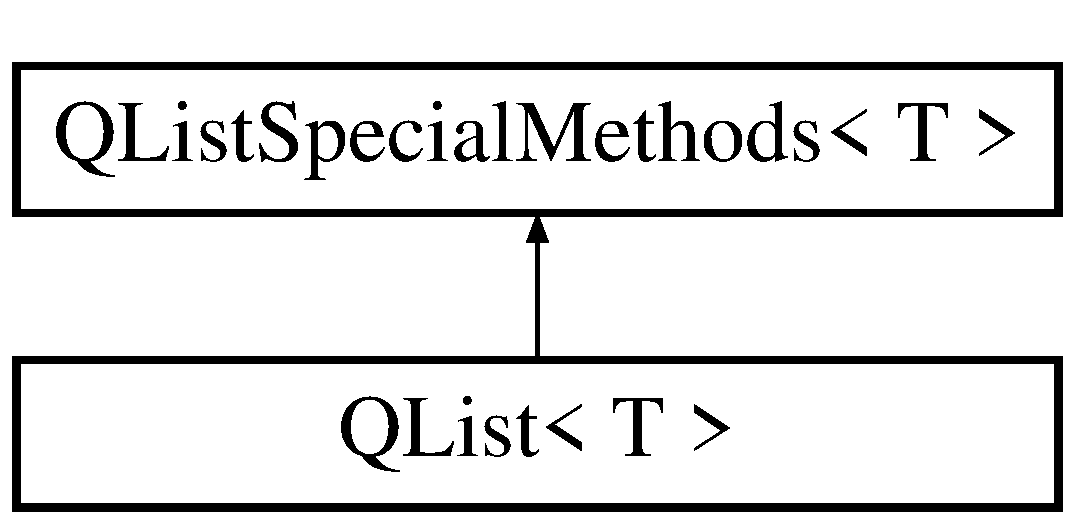
\includegraphics[height=2.000000cm]{struct_q_list_special_methods}
\end{center}
\end{figure}
\subsection*{Protected Member Functions}
\begin{DoxyCompactItemize}
\item 
\hyperlink{struct_q_list_special_methods_a15e29a889b231d220585ed597e341374}{$\sim$\+Q\+List\+Special\+Methods} ()
\end{DoxyCompactItemize}


\subsection{Detailed Description}
\subsubsection*{template$<$typename T$>$\\*
struct Q\+List\+Special\+Methods$<$ T $>$}



Definition at line 65 of file qlist.\+h.



\subsection{Constructor \& Destructor Documentation}
\index{Q\+List\+Special\+Methods@{Q\+List\+Special\+Methods}!````~Q\+List\+Special\+Methods@{$\sim$\+Q\+List\+Special\+Methods}}
\index{````~Q\+List\+Special\+Methods@{$\sim$\+Q\+List\+Special\+Methods}!Q\+List\+Special\+Methods@{Q\+List\+Special\+Methods}}
\subsubsection[{\texorpdfstring{$\sim$\+Q\+List\+Special\+Methods()}{~QListSpecialMethods()}}]{\setlength{\rightskip}{0pt plus 5cm}template$<$typename T$>$ {\bf Q\+List\+Special\+Methods}$<$ T $>$\+::$\sim${\bf Q\+List\+Special\+Methods} (
\begin{DoxyParamCaption}
{}
\end{DoxyParamCaption}
)\hspace{0.3cm}{\ttfamily [inline]}, {\ttfamily [protected]}}\hypertarget{struct_q_list_special_methods_a15e29a889b231d220585ed597e341374}{}\label{struct_q_list_special_methods_a15e29a889b231d220585ed597e341374}


Definition at line 68 of file qlist.\+h.



The documentation for this struct was generated from the following file\+:\begin{DoxyCompactItemize}
\item 
docs/extra-\/files/\hyperlink{qlist_8h}{qlist.\+h}\end{DoxyCompactItemize}

\hypertarget{class_q_map}{}\section{Q\+Map$<$ Key, T $>$ Class Template Reference}
\label{class_q_map}\index{Q\+Map$<$ Key, T $>$@{Q\+Map$<$ Key, T $>$}}


The \hyperlink{class_q_map}{Q\+Map} class is a template class that provides a red-\/black-\/tree-\/based dictionary.  




{\ttfamily \#include $<$qmap.\+h$>$}

Inheritance diagram for Q\+Map$<$ Key, T $>$\+:\begin{figure}[H]
\begin{center}
\leavevmode
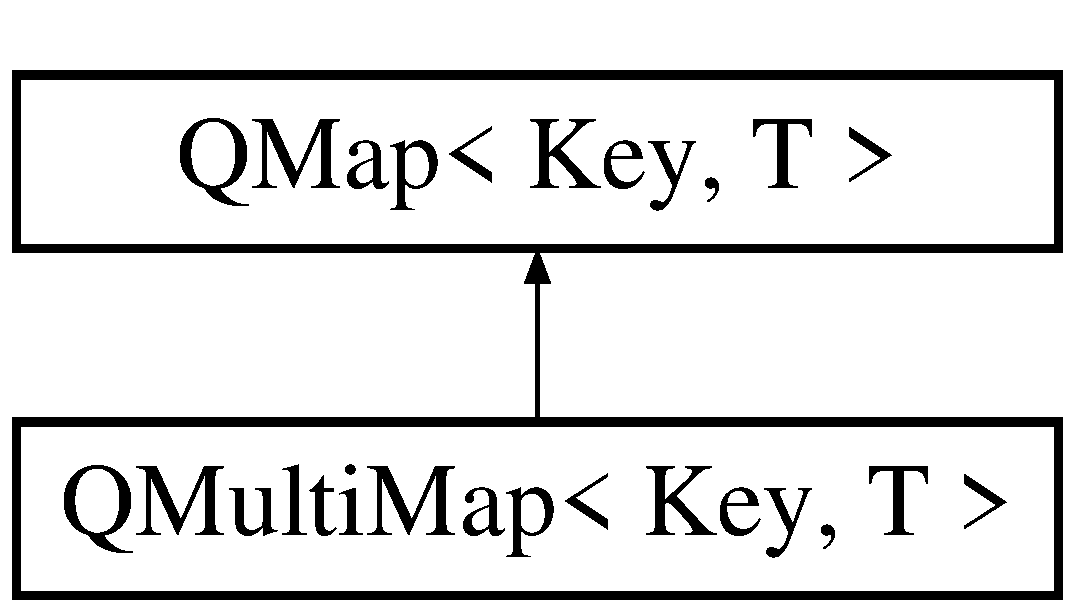
\includegraphics[height=2.000000cm]{class_q_map}
\end{center}
\end{figure}
\subsection*{Classes}
\begin{DoxyCompactItemize}
\item 
class \hyperlink{class_q_map_1_1const__iterator}{const\+\_\+iterator}
\begin{DoxyCompactList}\small\item\em The \hyperlink{class_q_map_1_1const__iterator}{Q\+Map\+::const\+\_\+iterator} class provides an S\+T\+L-\/style const iterator for \hyperlink{class_q_map}{Q\+Map} and \hyperlink{class_q_multi_map}{Q\+Multi\+Map}. \end{DoxyCompactList}\item 
class \hyperlink{class_q_map_1_1iterator}{iterator}
\begin{DoxyCompactList}\small\item\em The \hyperlink{class_q_map_1_1iterator}{Q\+Map\+::iterator} class provides an S\+T\+L-\/style non-\/const iterator for \hyperlink{class_q_map}{Q\+Map} and \hyperlink{class_q_multi_map}{Q\+Multi\+Map}. \end{DoxyCompactList}\end{DoxyCompactItemize}
\subsection*{Public Types}
\begin{DoxyCompactItemize}
\item 
typedef \hyperlink{class_q_map_1_1iterator}{iterator} \hyperlink{class_q_map_a1e3d75b555f8e9c0f8cf4043d179e15c}{Iterator}
\item 
typedef \hyperlink{class_q_map_1_1const__iterator}{const\+\_\+iterator} \hyperlink{class_q_map_ae0df3c69b27f3a8ceeab8244a59477ff}{Const\+Iterator}
\item 
typedef Key \hyperlink{class_q_map_aefd494f0aa5fde13a2740aa83ae33386}{key\+\_\+type}
\item 
typedef T \hyperlink{class_q_map_a8d473df53a41e0a8fb1f4490951b6f43}{mapped\+\_\+type}
\item 
typedef qptrdiff \hyperlink{class_q_map_a5f2bff0c8014b0b8142982d17728d0ca}{difference\+\_\+type}
\item 
typedef int \hyperlink{class_q_map_a6c8551f9c925b9e5dc73129fc1609c90}{size\+\_\+type}
\end{DoxyCompactItemize}
\subsection*{Public Member Functions}
\begin{DoxyCompactItemize}
\item 
\hyperlink{class_q_map_a72c9b87bd2e154fc1a0afc0bd6cc4223}{Q\+Map} ()
\item 
\hyperlink{class_q_map_ab4f75cfffb9554773b5fad068720f00e}{Q\+Map} (const \hyperlink{class_q_map}{Q\+Map}$<$ Key, T $>$ \&other)
\item 
\hyperlink{class_q_map_aa171c2af7b745664c156055dc53a3929}{$\sim$\+Q\+Map} ()
\item 
\hyperlink{class_q_map}{Q\+Map}$<$ Key, T $>$ \& \hyperlink{class_q_map_ad04759cfb5b1ed0f3d35a2a16f45ae54}{operator=} (const \hyperlink{class_q_map}{Q\+Map}$<$ Key, T $>$ \&other)
\item 
void \hyperlink{class_q_map_ac85cda6eaaa3b14867da113f6f69acc3}{swap} (\hyperlink{class_q_map}{Q\+Map}$<$ Key, T $>$ \&other)
\item 
\hyperlink{class_q_map_a2ad69d3ba805cd31d586b26218f16dd6}{Q\+Map} (const typename std\+::map$<$ Key, T $>$ \&other)
\item 
std\+::map$<$ Key, T $>$ \hyperlink{class_q_map_aafa61193d3960d804719c2e611533438}{to\+Std\+Map} () const 
\item 
bool \hyperlink{class_q_map_afe77d0e5e8feb53142b48b2e9ec8b7fa}{operator==} (const \hyperlink{class_q_map}{Q\+Map}$<$ Key, T $>$ \&other) const 
\item 
bool \hyperlink{class_q_map_a0e25c738535f0c64fe684d7e89097d57}{operator!=} (const \hyperlink{class_q_map}{Q\+Map}$<$ Key, T $>$ \&other) const 
\item 
int \hyperlink{class_q_map_a1e80b0b61a702ec2996f6a3d01425108}{size} () const 
\item 
bool \hyperlink{class_q_map_a33cfb24195273a5e70dcc48644368a99}{is\+Empty} () const 
\item 
void \hyperlink{class_q_map_a6913ba3a784e35a4b0d274f229af92ea}{detach} ()
\item 
bool \hyperlink{class_q_map_a0386f837a8b99aca59b01d7c5d04b202}{is\+Detached} () const 
\item 
bool \hyperlink{class_q_map_ae5cfba01ae8fc15b7b05ccc76129385f}{is\+Shared\+With} (const \hyperlink{class_q_map}{Q\+Map}$<$ Key, T $>$ \&other) const 
\item 
void \hyperlink{class_q_map_acdbbd64e3cd0a6dae1ac57c1d41aacab}{clear} ()
\item 
int \hyperlink{class_q_map_af562610e90763fad449dfc130bd18fb8}{remove} (const Key \&\hyperlink{class_q_map_a7ad0c404885c5287fe593849e4bc80d6}{key})
\item 
T \hyperlink{class_q_map_ac6f3e69396c5665d24d8b25bdf4e5ae7}{take} (const Key \&\hyperlink{class_q_map_a7ad0c404885c5287fe593849e4bc80d6}{key})
\item 
bool \hyperlink{class_q_map_ac92f0cafb70425a2d3d5171cf367dd11}{contains} (const Key \&\hyperlink{class_q_map_a7ad0c404885c5287fe593849e4bc80d6}{key}) const 
\item 
const Key \hyperlink{class_q_map_a7ad0c404885c5287fe593849e4bc80d6}{key} (const T \&\hyperlink{class_q_map_ab9c04f61f4abd94439d4431118a238e5}{value}, const Key \&default\+Key=Key()) const 
\item 
const T \hyperlink{class_q_map_ab9c04f61f4abd94439d4431118a238e5}{value} (const Key \&\hyperlink{class_q_map_a7ad0c404885c5287fe593849e4bc80d6}{key}, const T \&default\+Value=T()) const 
\item 
T \& \hyperlink{class_q_map_a69dc3a1b9dde2e59e829a7baa9761bc7}{operator\mbox{[}$\,$\mbox{]}} (const Key \&\hyperlink{class_q_map_a7ad0c404885c5287fe593849e4bc80d6}{key})
\item 
const T \hyperlink{class_q_map_a17e56b01b24614bb30e500f6fffb0cf8}{operator\mbox{[}$\,$\mbox{]}} (const Key \&\hyperlink{class_q_map_a7ad0c404885c5287fe593849e4bc80d6}{key}) const 
\item 
\hyperlink{class_q_list}{Q\+List}$<$ Key $>$ \hyperlink{class_q_map_a741722c285b32c3c6e59b3d5c89b2177}{unique\+Keys} () const 
\item 
\hyperlink{class_q_list}{Q\+List}$<$ Key $>$ \hyperlink{class_q_map_a12b7cde7eb217194ceff17bc44e93a93}{keys} () const 
\item 
\hyperlink{class_q_list}{Q\+List}$<$ Key $>$ \hyperlink{class_q_map_ab0a66ce475c7d00a706c673ba6c36697}{keys} (const T \&\hyperlink{class_q_map_ab9c04f61f4abd94439d4431118a238e5}{value}) const 
\item 
\hyperlink{class_q_list}{Q\+List}$<$ T $>$ \hyperlink{class_q_map_a86b7de4427e1a5e09cd6064d92209fd3}{values} () const 
\item 
\hyperlink{class_q_list}{Q\+List}$<$ T $>$ \hyperlink{class_q_map_ad3b4a80945a3159cde215d40931a509c}{values} (const Key \&\hyperlink{class_q_map_a7ad0c404885c5287fe593849e4bc80d6}{key}) const 
\item 
int \hyperlink{class_q_map_a7576304b0025dbb0f127c655c05377ac}{count} (const Key \&\hyperlink{class_q_map_a7ad0c404885c5287fe593849e4bc80d6}{key}) const 
\item 
const Key \& \hyperlink{class_q_map_a21b63de8c6e2acf6458e1f037447f1f1}{first\+Key} () const 
\item 
const Key \& \hyperlink{class_q_map_adf18d1ecc5ba94a47d7aed1c76a9a02e}{last\+Key} () const 
\item 
T \& \hyperlink{class_q_map_a76eff2973b6f43136f19c4ece9b26e20}{first} ()
\item 
const T \& \hyperlink{class_q_map_ada606e964f8103db2aa394f13c9739a5}{first} () const 
\item 
T \& \hyperlink{class_q_map_a15760303547971e1b447b9c101c11c8d}{last} ()
\item 
const T \& \hyperlink{class_q_map_af87415f175b4695209630b0d3f5a092b}{last} () const 
\item 
\hyperlink{class_q_map_1_1iterator}{iterator} \hyperlink{class_q_map_a5712fc69379f2b6d707a1c65391ff9ef}{begin} ()
\item 
\hyperlink{class_q_map_1_1const__iterator}{const\+\_\+iterator} \hyperlink{class_q_map_ad68737610cafc03024bd38baeaf79497}{begin} () const 
\item 
\hyperlink{class_q_map_1_1const__iterator}{const\+\_\+iterator} \hyperlink{class_q_map_ab55b01ac2790d09ceff0b911474a8b43}{const\+Begin} () const 
\item 
\hyperlink{class_q_map_1_1const__iterator}{const\+\_\+iterator} \hyperlink{class_q_map_a47aabac432ee8118f320217fd53ea32e}{cbegin} () const 
\item 
\hyperlink{class_q_map_1_1iterator}{iterator} \hyperlink{class_q_map_a2935881385191efbb074e96cf8d3c9b6}{end} ()
\item 
\hyperlink{class_q_map_1_1const__iterator}{const\+\_\+iterator} \hyperlink{class_q_map_abacc17da153723c386eb2c280460718f}{end} () const 
\item 
\hyperlink{class_q_map_1_1const__iterator}{const\+\_\+iterator} \hyperlink{class_q_map_a6307f2d58e928bb15019024150f0afcb}{const\+End} () const 
\item 
\hyperlink{class_q_map_1_1const__iterator}{const\+\_\+iterator} \hyperlink{class_q_map_a51c894aba21c16d3b778f211a43d9ee0}{cend} () const 
\item 
\hyperlink{class_q_map_1_1iterator}{iterator} \hyperlink{class_q_map_add6cad4f0b12644cfe593d95f7a75807}{erase} (\hyperlink{class_q_map_1_1iterator}{iterator} it)
\item 
int \hyperlink{class_q_map_ab80b18b6941bf11916918741a7342263}{count} () const 
\item 
\hyperlink{class_q_map_1_1iterator}{iterator} \hyperlink{class_q_map_a8cf44b635018eb178cc724ed20379d85}{find} (const Key \&\hyperlink{class_q_map_a7ad0c404885c5287fe593849e4bc80d6}{key})
\item 
\hyperlink{class_q_map_1_1const__iterator}{const\+\_\+iterator} \hyperlink{class_q_map_a0039730f5b5bb80ef4937d5a798f96c0}{find} (const Key \&\hyperlink{class_q_map_a7ad0c404885c5287fe593849e4bc80d6}{key}) const 
\item 
\hyperlink{class_q_map_1_1const__iterator}{const\+\_\+iterator} \hyperlink{class_q_map_a4777a4aa1616ea8443c8b66bce74602f}{const\+Find} (const Key \&\hyperlink{class_q_map_a7ad0c404885c5287fe593849e4bc80d6}{key}) const 
\item 
\hyperlink{class_q_map_1_1iterator}{iterator} \hyperlink{class_q_map_a7c26eec01e2b6053993018f710ff794c}{lower\+Bound} (const Key \&\hyperlink{class_q_map_a7ad0c404885c5287fe593849e4bc80d6}{key})
\item 
\hyperlink{class_q_map_1_1const__iterator}{const\+\_\+iterator} \hyperlink{class_q_map_a39bab49063dee3a17e004666e72b4993}{lower\+Bound} (const Key \&\hyperlink{class_q_map_a7ad0c404885c5287fe593849e4bc80d6}{key}) const 
\item 
\hyperlink{class_q_map_1_1iterator}{iterator} \hyperlink{class_q_map_abb757580db388ce382c6b50670f819b4}{upper\+Bound} (const Key \&\hyperlink{class_q_map_a7ad0c404885c5287fe593849e4bc80d6}{key})
\item 
\hyperlink{class_q_map_1_1const__iterator}{const\+\_\+iterator} \hyperlink{class_q_map_a6efc980cc3b0a1dd688aafa7ab08a39d}{upper\+Bound} (const Key \&\hyperlink{class_q_map_a7ad0c404885c5287fe593849e4bc80d6}{key}) const 
\item 
\hyperlink{class_q_map_1_1iterator}{iterator} \hyperlink{class_q_map_a0cc56ab47ea14af1127ac7399814d289}{insert} (const Key \&\hyperlink{class_q_map_a7ad0c404885c5287fe593849e4bc80d6}{key}, const T \&\hyperlink{class_q_map_ab9c04f61f4abd94439d4431118a238e5}{value})
\item 
\hyperlink{class_q_map_1_1iterator}{iterator} \hyperlink{class_q_map_a60a6aec6ecf27fc24390af0f4fe59ba4}{insert} (\hyperlink{class_q_map_1_1const__iterator}{const\+\_\+iterator} pos, const Key \&\hyperlink{class_q_map_a7ad0c404885c5287fe593849e4bc80d6}{key}, const T \&\hyperlink{class_q_map_ab9c04f61f4abd94439d4431118a238e5}{value})
\item 
\hyperlink{class_q_map_1_1iterator}{iterator} \hyperlink{class_q_map_a075634da2cf912a20dd1c4a5835acfa3}{insert\+Multi} (const Key \&\hyperlink{class_q_map_a7ad0c404885c5287fe593849e4bc80d6}{key}, const T \&\hyperlink{class_q_map_ab9c04f61f4abd94439d4431118a238e5}{value})
\item 
\hyperlink{class_q_map_1_1iterator}{iterator} \hyperlink{class_q_map_ae3083c5d69f5792346d3e3ea29c12eb8}{insert\+Multi} (\hyperlink{class_q_map_1_1const__iterator}{const\+\_\+iterator} pos, const Key \&akey, const T \&avalue)
\item 
\hyperlink{class_q_map}{Q\+Map}$<$ Key, T $>$ \& \hyperlink{class_q_map_a4626753159700253f441ad14fdc12245}{unite} (const \hyperlink{class_q_map}{Q\+Map}$<$ Key, T $>$ \&other)
\item 
bool \hyperlink{class_q_map_a69fbff17a8cde71f44ecafbdb4c1c4e2}{empty} () const 
\item 
Q\+Pair$<$ \hyperlink{class_q_map_1_1iterator}{iterator}, \hyperlink{class_q_map_1_1iterator}{iterator} $>$ \hyperlink{class_q_map_a5d475ecfb48fba208a560e4e7139ed77}{equal\+\_\+range} (const Key \&akey)
\end{DoxyCompactItemize}
\subsection*{Friends}
\begin{DoxyCompactItemize}
\item 
class \hyperlink{class_q_map_a67171474c4da6cc8efe0c7fafefd2b2d}{iterator}
\item 
class \hyperlink{class_q_map_ac220ce1c155db1ac44146c12d178056f}{const\+\_\+iterator}
\end{DoxyCompactItemize}
\subsection*{Related Functions}
(Note that these are not member functions.) \begin{DoxyCompactItemize}
\item 
Q\+Data\+Stream \& \hyperlink{class_q_map_a4ab8793bbdb9c841c4dfccd174f8bd52}{operator$<$$<$} (Q\+Data\+Stream \&out, const \hyperlink{class_q_map}{Q\+Map}$<$ Key, T $>$ \&map)
\item 
Q\+Data\+Stream \& \hyperlink{class_q_map_af84c5c06c005047bb65a8c36edde06d0}{operator$>$$>$} (Q\+Data\+Stream \&in, \hyperlink{class_q_map}{Q\+Map}$<$ Key, T $>$ \&map)
\end{DoxyCompactItemize}


\subsection{Detailed Description}
\subsubsection*{template$<$class Key, class T$>$\\*
class Q\+Map$<$ Key, T $>$}

The \hyperlink{class_q_map}{Q\+Map} class is a template class that provides a red-\/black-\/tree-\/based dictionary. 

Qt\+Core

\hyperlink{class_q_map}{Q\+Map}$<$Key, T$>$ is one of Qt\textquotesingle{}s generic \{container classes\}. It stores (key, value) pairs and provides fast lookup of the value associated with a key.

\hyperlink{class_q_map}{Q\+Map} and Q\+Hash provide very similar functionality. The differences are\+:

\begin{DoxyItemize}
\item Q\+Hash provides average faster lookups than \hyperlink{class_q_map}{Q\+Map}. (See \{Algorithmic Complexity\} for details.) \item When iterating over a Q\+Hash, the items are arbitrarily ordered. With \hyperlink{class_q_map}{Q\+Map}, the items are always sorted by key. \item The key type of a Q\+Hash must provide \hyperlink{class_q_map_afe77d0e5e8feb53142b48b2e9ec8b7fa}{operator==()} and a global q\+Hash(\+Key) function. The key type of a \hyperlink{class_q_map}{Q\+Map} must provide operator$<$() specifying a total order. \end{DoxyItemize}
Here\textquotesingle{}s an example \hyperlink{class_q_map}{Q\+Map} with Q\+String keys and {\ttfamily int} values\+: 
\begin{DoxyCodeInclude}
\end{DoxyCodeInclude}
 To insert a (key, value) pair into the map, you can use \hyperlink{class_q_map_a69dc3a1b9dde2e59e829a7baa9761bc7}{operator\mbox{[}$\,$\mbox{]}()}\+:


\begin{DoxyCodeInclude}
\end{DoxyCodeInclude}
 This inserts the following three (key, value) pairs into the \hyperlink{class_q_map}{Q\+Map}\+: (\char`\"{}one\char`\"{}, 1), (\char`\"{}three\char`\"{}, 3), and (\char`\"{}seven\char`\"{}, 7). Another way to insert items into the map is to use \hyperlink{class_q_map_a0cc56ab47ea14af1127ac7399814d289}{insert()}\+:


\begin{DoxyCodeInclude}
\end{DoxyCodeInclude}
 To look up a value, use \hyperlink{class_q_map_a69dc3a1b9dde2e59e829a7baa9761bc7}{operator\mbox{[}$\,$\mbox{]}()} or \hyperlink{class_q_map_ab9c04f61f4abd94439d4431118a238e5}{value()}\+:


\begin{DoxyCodeInclude}
\end{DoxyCodeInclude}
 If there is no item with the specified key in the map, these functions return a \{default-\/constructed value\}.

If you want to check whether the map contains a certain key, use \hyperlink{class_q_map_ac92f0cafb70425a2d3d5171cf367dd11}{contains()}\+:


\begin{DoxyCodeInclude}
\end{DoxyCodeInclude}
 There is also a \hyperlink{class_q_map_ab9c04f61f4abd94439d4431118a238e5}{value()} overload that uses its second argument as a default value if there is no item with the specified key\+:


\begin{DoxyCodeInclude}
\end{DoxyCodeInclude}
 In general, we recommend that you use \hyperlink{class_q_map_ac92f0cafb70425a2d3d5171cf367dd11}{contains()} and \hyperlink{class_q_map_ab9c04f61f4abd94439d4431118a238e5}{value()} rather than \hyperlink{class_q_map_a69dc3a1b9dde2e59e829a7baa9761bc7}{operator\mbox{[}$\,$\mbox{]}()} for looking up a key in a map. The reason is that \hyperlink{class_q_map_a69dc3a1b9dde2e59e829a7baa9761bc7}{operator\mbox{[}$\,$\mbox{]}()} silently inserts an item into the map if no item exists with the same key (unless the map is const). For example, the following code snippet will create 1000 items in memory\+:


\begin{DoxyCodeInclude}
\end{DoxyCodeInclude}
 To avoid this problem, replace {\ttfamily map}\mbox{[}i\mbox{]} with {\ttfamily map.\+value(i)} in the code above.

If you want to navigate through all the (key, value) pairs stored in a \hyperlink{class_q_map}{Q\+Map}, you can use an iterator. \hyperlink{class_q_map}{Q\+Map} provides both \{Java-\/style iterators\} (Q\+Map\+Iterator and Q\+Mutable\+Map\+Iterator) and \{S\+T\+L-\/style iterators\} (\hyperlink{class_q_map_1_1const__iterator}{Q\+Map\+::const\+\_\+iterator} and \hyperlink{class_q_map_1_1iterator}{Q\+Map\+::iterator}). Here\textquotesingle{}s how to iterate over a \hyperlink{class_q_map}{Q\+Map$<$\+Q\+String, int$>$} using a Java-\/style iterator\+:


\begin{DoxyCodeInclude}
\end{DoxyCodeInclude}
 Here\textquotesingle{}s the same code, but using an S\+T\+L-\/style iterator this time\+:


\begin{DoxyCodeInclude}
\end{DoxyCodeInclude}
 The items are traversed in ascending key order.

Normally, a \hyperlink{class_q_map}{Q\+Map} allows only one value per key. If you call \hyperlink{class_q_map_a0cc56ab47ea14af1127ac7399814d289}{insert()} with a key that already exists in the \hyperlink{class_q_map}{Q\+Map}, the previous value will be erased. For example\+:


\begin{DoxyCodeInclude}
\end{DoxyCodeInclude}
 However, you can store multiple values per key by using \hyperlink{class_q_map_a075634da2cf912a20dd1c4a5835acfa3}{insert\+Multi()} instead of \hyperlink{class_q_map_a0cc56ab47ea14af1127ac7399814d289}{insert()} (or using the convenience subclass \hyperlink{class_q_multi_map}{Q\+Multi\+Map}). If you want to retrieve all the values for a single key, you can use values(const Key \&key), which returns a Q\+List$<$\+T$>$\+:


\begin{DoxyCodeInclude}
\end{DoxyCodeInclude}
 The items that share the same key are available from most recently to least recently inserted. Another approach is to call \hyperlink{class_q_map_a8cf44b635018eb178cc724ed20379d85}{find()} to get the S\+T\+L-\/style iterator for the first item with a key and iterate from there\+:


\begin{DoxyCodeInclude}
\end{DoxyCodeInclude}
 If you only need to extract the values from a map (not the keys), you can also use \{foreach\}\+:


\begin{DoxyCodeInclude}
\end{DoxyCodeInclude}
 Items can be removed from the map in several ways. One way is to call \hyperlink{class_q_map_af562610e90763fad449dfc130bd18fb8}{remove()}; this will remove any item with the given key. Another way is to use Q\+Mutable\+Map\+Iterator\+::remove(). In addition, you can clear the entire map using \hyperlink{class_q_map_acdbbd64e3cd0a6dae1ac57c1d41aacab}{clear()}.

\hyperlink{class_q_map}{Q\+Map}\textquotesingle{}s key and value data types must be \{assignable data types\}. This covers most data types you are likely to encounter, but the compiler won\textquotesingle{}t let you, for example, store a Q\+Widget as a value; instead, store a Q\+Widget $\ast$. In addition, \hyperlink{class_q_map}{Q\+Map}\textquotesingle{}s key type must provide operator$<$(). \hyperlink{class_q_map}{Q\+Map} uses it to keep its items sorted, and assumes that two keys {\ttfamily x} and {\ttfamily y} are equal if neither {\ttfamily }\{x $<$ y\} nor {\ttfamily }\{y $<$ x\} is true.

Example\+: 
\begin{DoxyCodeInclude}
\end{DoxyCodeInclude}
 In the example, we start by comparing the employees\textquotesingle{} names. If they\textquotesingle{}re equal, we compare their dates of birth to break the tie.

\begin{DoxySeeAlso}{See also}
Q\+Map\+Iterator, Q\+Mutable\+Map\+Iterator, Q\+Hash, \hyperlink{class_q_set}{Q\+Set} 
\end{DoxySeeAlso}


Definition at line 321 of file qmap.\+h.



\subsection{Member Typedef Documentation}
\index{Q\+Map@{Q\+Map}!Const\+Iterator@{Const\+Iterator}}
\index{Const\+Iterator@{Const\+Iterator}!Q\+Map@{Q\+Map}}
\subsubsection[{\texorpdfstring{Const\+Iterator}{ConstIterator}}]{\setlength{\rightskip}{0pt plus 5cm}template$<$class Key, class T$>$ {\bf Q\+Map}$<$ Key, T $>$\+::{\bf Const\+Iterator}}\hypertarget{class_q_map_ae0df3c69b27f3a8ceeab8244a59477ff}{}\label{class_q_map_ae0df3c69b27f3a8ceeab8244a59477ff}
Qt-\/style synonym for \hyperlink{class_q_map_1_1const__iterator}{Q\+Map\+::const\+\_\+iterator}. 

Definition at line 538 of file qmap.\+h.

\index{Q\+Map@{Q\+Map}!difference\+\_\+type@{difference\+\_\+type}}
\index{difference\+\_\+type@{difference\+\_\+type}!Q\+Map@{Q\+Map}}
\subsubsection[{\texorpdfstring{difference\+\_\+type}{difference_type}}]{\setlength{\rightskip}{0pt plus 5cm}template$<$class Key, class T$>$ {\bf Q\+Map}$<$ Key, T $>$\+::{\bf difference\+\_\+type}}\hypertarget{class_q_map_a5f2bff0c8014b0b8142982d17728d0ca}{}\label{class_q_map_a5f2bff0c8014b0b8142982d17728d0ca}
Typedef for ptrdiff\+\_\+t. Provided for S\+TL compatibility. 

Definition at line 556 of file qmap.\+h.

\index{Q\+Map@{Q\+Map}!Iterator@{Iterator}}
\index{Iterator@{Iterator}!Q\+Map@{Q\+Map}}
\subsubsection[{\texorpdfstring{Iterator}{Iterator}}]{\setlength{\rightskip}{0pt plus 5cm}template$<$class Key, class T$>$ {\bf Q\+Map}$<$ Key, T $>$\+::{\bf Iterator}}\hypertarget{class_q_map_a1e3d75b555f8e9c0f8cf4043d179e15c}{}\label{class_q_map_a1e3d75b555f8e9c0f8cf4043d179e15c}
Qt-\/style synonym for \hyperlink{class_q_map_1_1iterator}{Q\+Map\+::iterator}. 

Definition at line 537 of file qmap.\+h.

\index{Q\+Map@{Q\+Map}!key\+\_\+type@{key\+\_\+type}}
\index{key\+\_\+type@{key\+\_\+type}!Q\+Map@{Q\+Map}}
\subsubsection[{\texorpdfstring{key\+\_\+type}{key_type}}]{\setlength{\rightskip}{0pt plus 5cm}template$<$class Key, class T$>$ {\bf Q\+Map}$<$ Key, T $>$\+::{\bf key\+\_\+type}}\hypertarget{class_q_map_aefd494f0aa5fde13a2740aa83ae33386}{}\label{class_q_map_aefd494f0aa5fde13a2740aa83ae33386}
Typedef for Key. Provided for S\+TL compatibility. 

Definition at line 554 of file qmap.\+h.

\index{Q\+Map@{Q\+Map}!mapped\+\_\+type@{mapped\+\_\+type}}
\index{mapped\+\_\+type@{mapped\+\_\+type}!Q\+Map@{Q\+Map}}
\subsubsection[{\texorpdfstring{mapped\+\_\+type}{mapped_type}}]{\setlength{\rightskip}{0pt plus 5cm}template$<$class Key, class T$>$ {\bf Q\+Map}$<$ Key, T $>$\+::{\bf mapped\+\_\+type}}\hypertarget{class_q_map_a8d473df53a41e0a8fb1f4490951b6f43}{}\label{class_q_map_a8d473df53a41e0a8fb1f4490951b6f43}
Typedef for T. Provided for S\+TL compatibility. 

Definition at line 555 of file qmap.\+h.

\index{Q\+Map@{Q\+Map}!size\+\_\+type@{size\+\_\+type}}
\index{size\+\_\+type@{size\+\_\+type}!Q\+Map@{Q\+Map}}
\subsubsection[{\texorpdfstring{size\+\_\+type}{size_type}}]{\setlength{\rightskip}{0pt plus 5cm}template$<$class Key, class T$>$ {\bf Q\+Map}$<$ Key, T $>$\+::{\bf size\+\_\+type}}\hypertarget{class_q_map_a6c8551f9c925b9e5dc73129fc1609c90}{}\label{class_q_map_a6c8551f9c925b9e5dc73129fc1609c90}
Typedef for int. Provided for S\+TL compatibility. 

Definition at line 557 of file qmap.\+h.



\subsection{Constructor \& Destructor Documentation}
\index{Q\+Map@{Q\+Map}!Q\+Map@{Q\+Map}}
\index{Q\+Map@{Q\+Map}!Q\+Map@{Q\+Map}}
\subsubsection[{\texorpdfstring{Q\+Map()}{QMap()}}]{\setlength{\rightskip}{0pt plus 5cm}template$<$class Key, class T$>$ {\bf Q\+Map}$<$ Key, T $>$\+::{\bf Q\+Map} (
\begin{DoxyParamCaption}
{}
\end{DoxyParamCaption}
)\hspace{0.3cm}{\ttfamily [inline]}}\hypertarget{class_q_map_a72c9b87bd2e154fc1a0afc0bd6cc4223}{}\label{class_q_map_a72c9b87bd2e154fc1a0afc0bd6cc4223}
Constructs an empty map.

\begin{DoxySeeAlso}{See also}
\hyperlink{class_q_map_acdbbd64e3cd0a6dae1ac57c1d41aacab}{clear()} 
\end{DoxySeeAlso}


Definition at line 328 of file qmap.\+h.

\index{Q\+Map@{Q\+Map}!Q\+Map@{Q\+Map}}
\index{Q\+Map@{Q\+Map}!Q\+Map@{Q\+Map}}
\subsubsection[{\texorpdfstring{Q\+Map(const Q\+Map$<$ Key, T $>$ \&other)}{QMap(const QMap< Key, T > &other)}}]{\setlength{\rightskip}{0pt plus 5cm}template$<$class Key, class T$>$ {\bf Q\+Map}$<$ Key, T $>$\+::{\bf Q\+Map} (
\begin{DoxyParamCaption}
\item[{const {\bf Q\+Map}$<$ Key, T $>$ \&}]{other}
\end{DoxyParamCaption}
)\hspace{0.3cm}{\ttfamily [inline]}}\hypertarget{class_q_map_ab4f75cfffb9554773b5fad068720f00e}{}\label{class_q_map_ab4f75cfffb9554773b5fad068720f00e}
Constructs a copy of {\itshape other}.

This operation occurs in \{constant time\}, because \hyperlink{class_q_map}{Q\+Map} is \{implicitly shared\}. This makes returning a \hyperlink{class_q_map}{Q\+Map} from a function very fast. If a shared instance is modified, it will be copied (copy-\/on-\/write), and this takes \{linear time\}.

\begin{DoxySeeAlso}{See also}
\hyperlink{class_q_map_ad04759cfb5b1ed0f3d35a2a16f45ae54}{operator=()} 
\end{DoxySeeAlso}


Definition at line 582 of file qmap.\+h.

\index{Q\+Map@{Q\+Map}!````~Q\+Map@{$\sim$\+Q\+Map}}
\index{````~Q\+Map@{$\sim$\+Q\+Map}!Q\+Map@{Q\+Map}}
\subsubsection[{\texorpdfstring{$\sim$\+Q\+Map()}{~QMap()}}]{\setlength{\rightskip}{0pt plus 5cm}template$<$class Key, class T$>$ {\bf Q\+Map}$<$ Key, T $>$\+::$\sim${\bf Q\+Map} (
\begin{DoxyParamCaption}
{}
\end{DoxyParamCaption}
)\hspace{0.3cm}{\ttfamily [inline]}}\hypertarget{class_q_map_aa171c2af7b745664c156055dc53a3929}{}\label{class_q_map_aa171c2af7b745664c156055dc53a3929}
Destroys the map. References to the values in the map, and all iterators over this map, become invalid. 

Definition at line 339 of file qmap.\+h.

\index{Q\+Map@{Q\+Map}!Q\+Map@{Q\+Map}}
\index{Q\+Map@{Q\+Map}!Q\+Map@{Q\+Map}}
\subsubsection[{\texorpdfstring{Q\+Map(const typename std\+::map$<$ Key, T $>$ \&other)}{QMap(const typename std::map< Key, T > &other)}}]{\setlength{\rightskip}{0pt plus 5cm}template$<$class Key, class T$>$ {\bf Q\+Map}$<$ Key, T $>$\+::{\bf Q\+Map} (
\begin{DoxyParamCaption}
\item[{const typename std\+::map$<$ Key, T $>$ \&}]{other}
\end{DoxyParamCaption}
)\hspace{0.3cm}{\ttfamily [explicit]}}\hypertarget{class_q_map_a2ad69d3ba805cd31d586b26218f16dd6}{}\label{class_q_map_a2ad69d3ba805cd31d586b26218f16dd6}


\subsection{Member Function Documentation}
\index{Q\+Map@{Q\+Map}!begin@{begin}}
\index{begin@{begin}!Q\+Map@{Q\+Map}}
\subsubsection[{\texorpdfstring{begin()}{begin()}}]{\setlength{\rightskip}{0pt plus 5cm}template$<$class Key, class T$>$ {\bf Q\+Map\+::iterator} {\bf Q\+Map}$<$ Key, T $>$\+::begin (
\begin{DoxyParamCaption}
{}
\end{DoxyParamCaption}
)\hspace{0.3cm}{\ttfamily [inline]}}\hypertarget{class_q_map_a5712fc69379f2b6d707a1c65391ff9ef}{}\label{class_q_map_a5712fc69379f2b6d707a1c65391ff9ef}
Returns an \{S\+T\+L-\/style iterators\}\{S\+T\+L-\/style iterator\} pointing to the first item in the map.

\begin{DoxySeeAlso}{See also}
\hyperlink{class_q_map_ab55b01ac2790d09ceff0b911474a8b43}{const\+Begin()}, \hyperlink{class_q_map_a2935881385191efbb074e96cf8d3c9b6}{end()} 
\end{DoxySeeAlso}


Definition at line 526 of file qmap.\+h.

\index{Q\+Map@{Q\+Map}!begin@{begin}}
\index{begin@{begin}!Q\+Map@{Q\+Map}}
\subsubsection[{\texorpdfstring{begin() const }{begin() const }}]{\setlength{\rightskip}{0pt plus 5cm}template$<$class Key, class T$>$ {\bf Q\+Map\+::const\+\_\+iterator} {\bf Q\+Map}$<$ Key, T $>$\+::begin (
\begin{DoxyParamCaption}
{}
\end{DoxyParamCaption}
) const\hspace{0.3cm}{\ttfamily [inline]}}\hypertarget{class_q_map_ad68737610cafc03024bd38baeaf79497}{}\label{class_q_map_ad68737610cafc03024bd38baeaf79497}
This is an overloaded member function, provided for convenience. It differs from the above function only in what argument(s) it accepts. 

Definition at line 527 of file qmap.\+h.

\index{Q\+Map@{Q\+Map}!cbegin@{cbegin}}
\index{cbegin@{cbegin}!Q\+Map@{Q\+Map}}
\subsubsection[{\texorpdfstring{cbegin() const }{cbegin() const }}]{\setlength{\rightskip}{0pt plus 5cm}template$<$class Key, class T$>$ {\bf Q\+Map\+::const\+\_\+iterator} {\bf Q\+Map}$<$ Key, T $>$\+::cbegin (
\begin{DoxyParamCaption}
{}
\end{DoxyParamCaption}
) const\hspace{0.3cm}{\ttfamily [inline]}}\hypertarget{class_q_map_a47aabac432ee8118f320217fd53ea32e}{}\label{class_q_map_a47aabac432ee8118f320217fd53ea32e}
\begin{DoxySince}{Since}
5.\+0
\end{DoxySince}
Returns a const \{S\+T\+L-\/style iterators\}\{S\+T\+L-\/style iterator\} pointing to the first item in the map.

\begin{DoxySeeAlso}{See also}
\hyperlink{class_q_map_a5712fc69379f2b6d707a1c65391ff9ef}{begin()}, \hyperlink{class_q_map_a51c894aba21c16d3b778f211a43d9ee0}{cend()} 
\end{DoxySeeAlso}


Definition at line 529 of file qmap.\+h.

\index{Q\+Map@{Q\+Map}!cend@{cend}}
\index{cend@{cend}!Q\+Map@{Q\+Map}}
\subsubsection[{\texorpdfstring{cend() const }{cend() const }}]{\setlength{\rightskip}{0pt plus 5cm}template$<$class Key, class T$>$ {\bf Q\+Map\+::const\+\_\+iterator} {\bf Q\+Map}$<$ Key, T $>$\+::cend (
\begin{DoxyParamCaption}
{}
\end{DoxyParamCaption}
) const\hspace{0.3cm}{\ttfamily [inline]}}\hypertarget{class_q_map_a51c894aba21c16d3b778f211a43d9ee0}{}\label{class_q_map_a51c894aba21c16d3b778f211a43d9ee0}
\begin{DoxySince}{Since}
5.\+0
\end{DoxySince}
Returns a const \{S\+T\+L-\/style iterators\}\{S\+T\+L-\/style iterator\} pointing to the imaginary item after the last item in the map.

\begin{DoxySeeAlso}{See also}
\hyperlink{class_q_map_a47aabac432ee8118f320217fd53ea32e}{cbegin()}, \hyperlink{class_q_map_a2935881385191efbb074e96cf8d3c9b6}{end()} 
\end{DoxySeeAlso}


Definition at line 533 of file qmap.\+h.

\index{Q\+Map@{Q\+Map}!clear@{clear}}
\index{clear@{clear}!Q\+Map@{Q\+Map}}
\subsubsection[{\texorpdfstring{clear()}{clear()}}]{\setlength{\rightskip}{0pt plus 5cm}template$<$class Key , class T $>$ Q\+\_\+\+I\+N\+L\+I\+N\+E\+\_\+\+T\+E\+M\+P\+L\+A\+TE void {\bf Q\+Map}$<$ Key, T $>$\+::clear (
\begin{DoxyParamCaption}
{}
\end{DoxyParamCaption}
)}\hypertarget{class_q_map_acdbbd64e3cd0a6dae1ac57c1d41aacab}{}\label{class_q_map_acdbbd64e3cd0a6dae1ac57c1d41aacab}
Removes all items from the map.

\begin{DoxySeeAlso}{See also}
\hyperlink{class_q_map_af562610e90763fad449dfc130bd18fb8}{remove()} 
\end{DoxySeeAlso}


Definition at line 607 of file qmap.\+h.

\index{Q\+Map@{Q\+Map}!const\+Begin@{const\+Begin}}
\index{const\+Begin@{const\+Begin}!Q\+Map@{Q\+Map}}
\subsubsection[{\texorpdfstring{const\+Begin() const }{constBegin() const }}]{\setlength{\rightskip}{0pt plus 5cm}template$<$class Key, class T$>$ {\bf Q\+Map\+::const\+\_\+iterator} {\bf Q\+Map}$<$ Key, T $>$\+::const\+Begin (
\begin{DoxyParamCaption}
{}
\end{DoxyParamCaption}
) const\hspace{0.3cm}{\ttfamily [inline]}}\hypertarget{class_q_map_ab55b01ac2790d09ceff0b911474a8b43}{}\label{class_q_map_ab55b01ac2790d09ceff0b911474a8b43}
Returns a const \{S\+T\+L-\/style iterators\}\{S\+T\+L-\/style iterator\} pointing to the first item in the map.

\begin{DoxySeeAlso}{See also}
\hyperlink{class_q_map_a5712fc69379f2b6d707a1c65391ff9ef}{begin()}, \hyperlink{class_q_map_a6307f2d58e928bb15019024150f0afcb}{const\+End()} 
\end{DoxySeeAlso}


Definition at line 528 of file qmap.\+h.

\index{Q\+Map@{Q\+Map}!const\+End@{const\+End}}
\index{const\+End@{const\+End}!Q\+Map@{Q\+Map}}
\subsubsection[{\texorpdfstring{const\+End() const }{constEnd() const }}]{\setlength{\rightskip}{0pt plus 5cm}template$<$class Key, class T$>$ {\bf Q\+Map\+::const\+\_\+iterator} {\bf Q\+Map}$<$ Key, T $>$\+::const\+End (
\begin{DoxyParamCaption}
{}
\end{DoxyParamCaption}
) const\hspace{0.3cm}{\ttfamily [inline]}}\hypertarget{class_q_map_a6307f2d58e928bb15019024150f0afcb}{}\label{class_q_map_a6307f2d58e928bb15019024150f0afcb}
Returns a const \{S\+T\+L-\/style iterators\}\{S\+T\+L-\/style iterator\} pointing to the imaginary item after the last item in the map.

\begin{DoxySeeAlso}{See also}
\hyperlink{class_q_map_ab55b01ac2790d09ceff0b911474a8b43}{const\+Begin()}, \hyperlink{class_q_map_a2935881385191efbb074e96cf8d3c9b6}{end()} 
\end{DoxySeeAlso}


Definition at line 532 of file qmap.\+h.

\index{Q\+Map@{Q\+Map}!const\+Find@{const\+Find}}
\index{const\+Find@{const\+Find}!Q\+Map@{Q\+Map}}
\subsubsection[{\texorpdfstring{const\+Find(const Key \&key) const }{constFind(const Key &key) const }}]{\setlength{\rightskip}{0pt plus 5cm}template$<$class Key, class T $>$ Q\+\_\+\+I\+N\+L\+I\+N\+E\+\_\+\+T\+E\+M\+P\+L\+A\+TE {\bf Q\+Map}$<$ Key, T $>$\+::{\bf const\+\_\+iterator} {\bf Q\+Map}$<$ Key, T $>$\+::const\+Find (
\begin{DoxyParamCaption}
\item[{const Key \&}]{key}
\end{DoxyParamCaption}
) const}\hypertarget{class_q_map_a4777a4aa1616ea8443c8b66bce74602f}{}\label{class_q_map_a4777a4aa1616ea8443c8b66bce74602f}
\begin{DoxySince}{Since}
4.\+1
\end{DoxySince}
Returns an const iterator pointing to the item with key {\itshape key} in the map.

If the map contains no item with key {\itshape key}, the function returns \hyperlink{class_q_map_a6307f2d58e928bb15019024150f0afcb}{const\+End()}.

\begin{DoxySeeAlso}{See also}
\hyperlink{class_q_map_a8cf44b635018eb178cc724ed20379d85}{find()}, \hyperlink{class_q_multi_map_ab0c0991e1c637c400b0d874f4a05b5ef}{Q\+Multi\+Map\+::const\+Find()} 
\end{DoxySeeAlso}


Definition at line 825 of file qmap.\+h.

\index{Q\+Map@{Q\+Map}!contains@{contains}}
\index{contains@{contains}!Q\+Map@{Q\+Map}}
\subsubsection[{\texorpdfstring{contains(const Key \&key) const }{contains(const Key &key) const }}]{\setlength{\rightskip}{0pt plus 5cm}template$<$class Key, class T $>$ Q\+\_\+\+I\+N\+L\+I\+N\+E\+\_\+\+T\+E\+M\+P\+L\+A\+TE bool {\bf Q\+Map}$<$ Key, T $>$\+::contains (
\begin{DoxyParamCaption}
\item[{const Key \&}]{key}
\end{DoxyParamCaption}
) const}\hypertarget{class_q_map_ac92f0cafb70425a2d3d5171cf367dd11}{}\label{class_q_map_ac92f0cafb70425a2d3d5171cf367dd11}
Returns {\ttfamily true} if the map contains an item with key {\itshape key}; otherwise returns {\ttfamily false}.

\begin{DoxySeeAlso}{See also}
\hyperlink{class_q_map_a7576304b0025dbb0f127c655c05377ac}{count()}, \hyperlink{class_q_multi_map_ab240b90606e155eef7c80c2ea9cabe74}{Q\+Multi\+Map\+::contains()} 
\end{DoxySeeAlso}


Definition at line 654 of file qmap.\+h.

\index{Q\+Map@{Q\+Map}!count@{count}}
\index{count@{count}!Q\+Map@{Q\+Map}}
\subsubsection[{\texorpdfstring{count(const Key \&key) const }{count(const Key &key) const }}]{\setlength{\rightskip}{0pt plus 5cm}template$<$class Key, class T $>$ Q\+\_\+\+I\+N\+L\+I\+N\+E\+\_\+\+T\+E\+M\+P\+L\+A\+TE int {\bf Q\+Map}$<$ Key, T $>$\+::count (
\begin{DoxyParamCaption}
\item[{const Key \&}]{key}
\end{DoxyParamCaption}
) const}\hypertarget{class_q_map_a7576304b0025dbb0f127c655c05377ac}{}\label{class_q_map_a7576304b0025dbb0f127c655c05377ac}
Returns the number of items associated with key {\itshape key}.

\begin{DoxySeeAlso}{See also}
\hyperlink{class_q_map_ac92f0cafb70425a2d3d5171cf367dd11}{contains()}, \hyperlink{class_q_map_a075634da2cf912a20dd1c4a5835acfa3}{insert\+Multi()}, \hyperlink{class_q_multi_map_abb89579656320a453ea7c80b2702d8c5}{Q\+Multi\+Map\+::count()} 
\end{DoxySeeAlso}


Definition at line 637 of file qmap.\+h.

\index{Q\+Map@{Q\+Map}!count@{count}}
\index{count@{count}!Q\+Map@{Q\+Map}}
\subsubsection[{\texorpdfstring{count() const }{count() const }}]{\setlength{\rightskip}{0pt plus 5cm}template$<$class Key, class T$>$ int {\bf Q\+Map}$<$ Key, T $>$\+::count (
\begin{DoxyParamCaption}
{}
\end{DoxyParamCaption}
) const\hspace{0.3cm}{\ttfamily [inline]}}\hypertarget{class_q_map_ab80b18b6941bf11916918741a7342263}{}\label{class_q_map_ab80b18b6941bf11916918741a7342263}
This is an overloaded member function, provided for convenience. It differs from the above function only in what argument(s) it accepts.

Same as \hyperlink{class_q_map_a1e80b0b61a702ec2996f6a3d01425108}{size()}. 

Definition at line 539 of file qmap.\+h.

\index{Q\+Map@{Q\+Map}!detach@{detach}}
\index{detach@{detach}!Q\+Map@{Q\+Map}}
\subsubsection[{\texorpdfstring{detach()}{detach()}}]{\setlength{\rightskip}{0pt plus 5cm}template$<$class Key, class T$>$ void {\bf Q\+Map}$<$ Key, T $>$\+::detach (
\begin{DoxyParamCaption}
{}
\end{DoxyParamCaption}
)\hspace{0.3cm}{\ttfamily [inline]}}\hypertarget{class_q_map_a6913ba3a784e35a4b0d274f229af92ea}{}\label{class_q_map_a6913ba3a784e35a4b0d274f229af92ea}


Definition at line 364 of file qmap.\+h.

\index{Q\+Map@{Q\+Map}!empty@{empty}}
\index{empty@{empty}!Q\+Map@{Q\+Map}}
\subsubsection[{\texorpdfstring{empty() const }{empty() const }}]{\setlength{\rightskip}{0pt plus 5cm}template$<$class Key, class T$>$ bool {\bf Q\+Map}$<$ Key, T $>$\+::empty (
\begin{DoxyParamCaption}
{}
\end{DoxyParamCaption}
) const\hspace{0.3cm}{\ttfamily [inline]}}\hypertarget{class_q_map_a69fbff17a8cde71f44ecafbdb4c1c4e2}{}\label{class_q_map_a69fbff17a8cde71f44ecafbdb4c1c4e2}
This function is provided for S\+TL compatibility. It is equivalent to \hyperlink{class_q_map_a33cfb24195273a5e70dcc48644368a99}{is\+Empty()}, returning true if the map is empty; otherwise returning false. 

Definition at line 558 of file qmap.\+h.

\index{Q\+Map@{Q\+Map}!end@{end}}
\index{end@{end}!Q\+Map@{Q\+Map}}
\subsubsection[{\texorpdfstring{end()}{end()}}]{\setlength{\rightskip}{0pt plus 5cm}template$<$class Key, class T$>$ {\bf Q\+Map\+::iterator} {\bf Q\+Map}$<$ Key, T $>$\+::end (
\begin{DoxyParamCaption}
{}
\end{DoxyParamCaption}
)\hspace{0.3cm}{\ttfamily [inline]}}\hypertarget{class_q_map_a2935881385191efbb074e96cf8d3c9b6}{}\label{class_q_map_a2935881385191efbb074e96cf8d3c9b6}
Returns an \{S\+T\+L-\/style iterators\}\{S\+T\+L-\/style iterator\} pointing to the imaginary item after the last item in the map.

\begin{DoxySeeAlso}{See also}
\hyperlink{class_q_map_a5712fc69379f2b6d707a1c65391ff9ef}{begin()}, \hyperlink{class_q_map_a6307f2d58e928bb15019024150f0afcb}{const\+End()} 
\end{DoxySeeAlso}


Definition at line 530 of file qmap.\+h.

\index{Q\+Map@{Q\+Map}!end@{end}}
\index{end@{end}!Q\+Map@{Q\+Map}}
\subsubsection[{\texorpdfstring{end() const }{end() const }}]{\setlength{\rightskip}{0pt plus 5cm}template$<$class Key, class T$>$ {\bf Q\+Map\+::const\+\_\+iterator} {\bf Q\+Map}$<$ Key, T $>$\+::end (
\begin{DoxyParamCaption}
{}
\end{DoxyParamCaption}
) const\hspace{0.3cm}{\ttfamily [inline]}}\hypertarget{class_q_map_abacc17da153723c386eb2c280460718f}{}\label{class_q_map_abacc17da153723c386eb2c280460718f}
This is an overloaded member function, provided for convenience. It differs from the above function only in what argument(s) it accepts. 

Definition at line 531 of file qmap.\+h.

\index{Q\+Map@{Q\+Map}!equal\+\_\+range@{equal\+\_\+range}}
\index{equal\+\_\+range@{equal\+\_\+range}!Q\+Map@{Q\+Map}}
\subsubsection[{\texorpdfstring{equal\+\_\+range(const Key \&akey)}{equal_range(const Key &akey)}}]{\setlength{\rightskip}{0pt plus 5cm}template$<$class Key, class T $>$ Q\+Pair$<$ typename {\bf Q\+Map}$<$ Key, T $>$\+::{\bf iterator}, typename {\bf Q\+Map}$<$ Key, T $>$\+::{\bf iterator} $>$ {\bf Q\+Map}$<$ Key, T $>$\+::equal\+\_\+range (
\begin{DoxyParamCaption}
\item[{const Key \&}]{key}
\end{DoxyParamCaption}
)}\hypertarget{class_q_map_a5d475ecfb48fba208a560e4e7139ed77}{}\label{class_q_map_a5d475ecfb48fba208a560e4e7139ed77}
Returns a pair of iterators delimiting the range of values that are stored under {\itshape key}. 

Definition at line 859 of file qmap.\+h.

\index{Q\+Map@{Q\+Map}!erase@{erase}}
\index{erase@{erase}!Q\+Map@{Q\+Map}}
\subsubsection[{\texorpdfstring{erase(iterator it)}{erase(iterator it)}}]{\setlength{\rightskip}{0pt plus 5cm}template$<$class Key , class T $>$ Q\+\_\+\+O\+U\+T\+O\+F\+L\+I\+N\+E\+\_\+\+T\+E\+M\+P\+L\+A\+TE {\bf Q\+Map}$<$ Key, T $>$\+::{\bf iterator} {\bf Q\+Map}$<$ Key, T $>$\+::erase (
\begin{DoxyParamCaption}
\item[{{\bf iterator}}]{pos}
\end{DoxyParamCaption}
)}\hypertarget{class_q_map_add6cad4f0b12644cfe593d95f7a75807}{}\label{class_q_map_add6cad4f0b12644cfe593d95f7a75807}
Removes the (key, value) pair pointed to by the iterator {\itshape pos} from the map, and returns an iterator to the next item in the map.

\begin{DoxySeeAlso}{See also}
\hyperlink{class_q_map_af562610e90763fad449dfc130bd18fb8}{remove()} 
\end{DoxySeeAlso}


Definition at line 916 of file qmap.\+h.

\index{Q\+Map@{Q\+Map}!find@{find}}
\index{find@{find}!Q\+Map@{Q\+Map}}
\subsubsection[{\texorpdfstring{find(const Key \&key)}{find(const Key &key)}}]{\setlength{\rightskip}{0pt plus 5cm}template$<$class Key, class T $>$ Q\+\_\+\+I\+N\+L\+I\+N\+E\+\_\+\+T\+E\+M\+P\+L\+A\+TE {\bf Q\+Map}$<$ Key, T $>$\+::{\bf iterator} {\bf Q\+Map}$<$ Key, T $>$\+::find (
\begin{DoxyParamCaption}
\item[{const Key \&}]{key}
\end{DoxyParamCaption}
)}\hypertarget{class_q_map_a8cf44b635018eb178cc724ed20379d85}{}\label{class_q_map_a8cf44b635018eb178cc724ed20379d85}
Returns an iterator pointing to the item with key {\itshape key} in the map.

If the map contains no item with key {\itshape key}, the function returns \hyperlink{class_q_map_a2935881385191efbb074e96cf8d3c9b6}{end()}.

If the map contains multiple items with key {\itshape key}, this function returns an iterator that points to the most recently inserted value. The other values are accessible by incrementing the iterator. For example, here\textquotesingle{}s some code that iterates over all the items with the same key\+:


\begin{DoxyCodeInclude}
\end{DoxyCodeInclude}
 \begin{DoxySeeAlso}{See also}
\hyperlink{class_q_map_a4777a4aa1616ea8443c8b66bce74602f}{const\+Find()}, \hyperlink{class_q_map_ab9c04f61f4abd94439d4431118a238e5}{value()}, \hyperlink{class_q_map_a86b7de4427e1a5e09cd6064d92209fd3}{values()}, \hyperlink{class_q_map_a7c26eec01e2b6053993018f710ff794c}{lower\+Bound()}, \hyperlink{class_q_map_abb757580db388ce382c6b50670f819b4}{upper\+Bound()}, \hyperlink{class_q_multi_map_ade33defb37a1abf5f4fff2686159afd4}{Q\+Multi\+Map\+::find()} 
\end{DoxySeeAlso}


Definition at line 838 of file qmap.\+h.

\index{Q\+Map@{Q\+Map}!find@{find}}
\index{find@{find}!Q\+Map@{Q\+Map}}
\subsubsection[{\texorpdfstring{find(const Key \&key) const }{find(const Key &key) const }}]{\setlength{\rightskip}{0pt plus 5cm}template$<$class Key, class T $>$ Q\+\_\+\+I\+N\+L\+I\+N\+E\+\_\+\+T\+E\+M\+P\+L\+A\+TE {\bf Q\+Map}$<$ Key, T $>$\+::{\bf const\+\_\+iterator} {\bf Q\+Map}$<$ Key, T $>$\+::find (
\begin{DoxyParamCaption}
\item[{const Key \&}]{key}
\end{DoxyParamCaption}
) const}\hypertarget{class_q_map_a0039730f5b5bb80ef4937d5a798f96c0}{}\label{class_q_map_a0039730f5b5bb80ef4937d5a798f96c0}
This is an overloaded member function, provided for convenience. It differs from the above function only in what argument(s) it accepts. 

Definition at line 832 of file qmap.\+h.

\index{Q\+Map@{Q\+Map}!first@{first}}
\index{first@{first}!Q\+Map@{Q\+Map}}
\subsubsection[{\texorpdfstring{first()}{first()}}]{\setlength{\rightskip}{0pt plus 5cm}template$<$class Key, class T$>$ T \& {\bf Q\+Map}$<$ Key, T $>$\+::first (
\begin{DoxyParamCaption}
{}
\end{DoxyParamCaption}
)\hspace{0.3cm}{\ttfamily [inline]}}\hypertarget{class_q_map_a76eff2973b6f43136f19c4ece9b26e20}{}\label{class_q_map_a76eff2973b6f43136f19c4ece9b26e20}
\begin{DoxySince}{Since}
5.\+2
\end{DoxySince}
Returns a reference to the first value in the map, that is the value mapped to the smallest key. This function assumes that the map is not empty.

When unshared (or const version is called), this executes in \{constant time\}.

\begin{DoxySeeAlso}{See also}
\hyperlink{class_q_map_a15760303547971e1b447b9c101c11c8d}{last()}, \hyperlink{class_q_map_a21b63de8c6e2acf6458e1f037447f1f1}{first\+Key()}, \hyperlink{class_q_map_a33cfb24195273a5e70dcc48644368a99}{is\+Empty()} 
\end{DoxySeeAlso}


Definition at line 400 of file qmap.\+h.

\index{Q\+Map@{Q\+Map}!first@{first}}
\index{first@{first}!Q\+Map@{Q\+Map}}
\subsubsection[{\texorpdfstring{first() const }{first() const }}]{\setlength{\rightskip}{0pt plus 5cm}template$<$class Key, class T$>$ const T \& {\bf Q\+Map}$<$ Key, T $>$\+::first (
\begin{DoxyParamCaption}
{}
\end{DoxyParamCaption}
) const\hspace{0.3cm}{\ttfamily [inline]}}\hypertarget{class_q_map_ada606e964f8103db2aa394f13c9739a5}{}\label{class_q_map_ada606e964f8103db2aa394f13c9739a5}
\begin{DoxySince}{Since}
5.\+2
\end{DoxySince}
This is an overloaded member function, provided for convenience. It differs from the above function only in what argument(s) it accepts. 

Definition at line 401 of file qmap.\+h.

\index{Q\+Map@{Q\+Map}!first\+Key@{first\+Key}}
\index{first\+Key@{first\+Key}!Q\+Map@{Q\+Map}}
\subsubsection[{\texorpdfstring{first\+Key() const }{firstKey() const }}]{\setlength{\rightskip}{0pt plus 5cm}template$<$class Key, class T$>$ const Key \& {\bf Q\+Map}$<$ Key, T $>$\+::first\+Key (
\begin{DoxyParamCaption}
{}
\end{DoxyParamCaption}
) const\hspace{0.3cm}{\ttfamily [inline]}}\hypertarget{class_q_map_a21b63de8c6e2acf6458e1f037447f1f1}{}\label{class_q_map_a21b63de8c6e2acf6458e1f037447f1f1}
\begin{DoxySince}{Since}
5.\+2
\end{DoxySince}
Returns a reference to the smallest key in the map. This function assumes that the map is not empty.

This executes in \{constant time\}.

\begin{DoxySeeAlso}{See also}
\hyperlink{class_q_map_adf18d1ecc5ba94a47d7aed1c76a9a02e}{last\+Key()}, \hyperlink{class_q_map_a76eff2973b6f43136f19c4ece9b26e20}{first()}, \hyperlink{class_q_map_a33cfb24195273a5e70dcc48644368a99}{is\+Empty()} 
\end{DoxySeeAlso}


Definition at line 397 of file qmap.\+h.

\index{Q\+Map@{Q\+Map}!insert@{insert}}
\index{insert@{insert}!Q\+Map@{Q\+Map}}
\subsubsection[{\texorpdfstring{insert(const Key \&key, const T \&value)}{insert(const Key &key, const T &value)}}]{\setlength{\rightskip}{0pt plus 5cm}template$<$class Key, class T$>$ Q\+\_\+\+I\+N\+L\+I\+N\+E\+\_\+\+T\+E\+M\+P\+L\+A\+TE {\bf Q\+Map}$<$ Key, T $>$\+::{\bf iterator} {\bf Q\+Map}$<$ Key, T $>$\+::insert (
\begin{DoxyParamCaption}
\item[{const Key \&}]{key, }
\item[{const T \&}]{value}
\end{DoxyParamCaption}
)}\hypertarget{class_q_map_a0cc56ab47ea14af1127ac7399814d289}{}\label{class_q_map_a0cc56ab47ea14af1127ac7399814d289}
Inserts a new item with the key {\itshape key} and a value of {\itshape value}.

If there is already an item with the key {\itshape key}, that item\textquotesingle{}s value is replaced with {\itshape value}.

If there are multiple items with the key {\itshape key}, the most recently inserted item\textquotesingle{}s value is replaced with {\itshape value}.

\begin{DoxySeeAlso}{See also}
\hyperlink{class_q_map_a075634da2cf912a20dd1c4a5835acfa3}{insert\+Multi()} 
\end{DoxySeeAlso}


Definition at line 660 of file qmap.\+h.

\index{Q\+Map@{Q\+Map}!insert@{insert}}
\index{insert@{insert}!Q\+Map@{Q\+Map}}
\subsubsection[{\texorpdfstring{insert(const\+\_\+iterator pos, const Key \&key, const T \&value)}{insert(const_iterator pos, const Key &key, const T &value)}}]{\setlength{\rightskip}{0pt plus 5cm}template$<$class Key, class T$>$ {\bf Q\+Map}$<$ Key, T $>$\+::{\bf iterator} {\bf Q\+Map}$<$ Key, T $>$\+::insert (
\begin{DoxyParamCaption}
\item[{{\bf const\+\_\+iterator}}]{pos, }
\item[{const Key \&}]{key, }
\item[{const T \&}]{value}
\end{DoxyParamCaption}
)}\hypertarget{class_q_map_a60a6aec6ecf27fc24390af0f4fe59ba4}{}\label{class_q_map_a60a6aec6ecf27fc24390af0f4fe59ba4}
This is an overloaded member function, provided for convenience. It differs from the above function only in what argument(s) it accepts. \begin{DoxySince}{Since}
5.\+1 Inserts a new item with the key {\itshape key} and value {\itshape value} and with hint {\itshape pos} suggesting where to do the insert.
\end{DoxySince}
If \hyperlink{class_q_map_ab55b01ac2790d09ceff0b911474a8b43}{const\+Begin()} is used as hint it indicates that the {\itshape key} is less than any key in the map while \hyperlink{class_q_map_a6307f2d58e928bb15019024150f0afcb}{const\+End()} suggests that the {\itshape key} is (strictly) larger than any key in the map. Otherwise the hint should meet the condition ({\itshape pos} -\/ 1).\hyperlink{class_q_map_a7ad0c404885c5287fe593849e4bc80d6}{key()} $<$ {\itshape key} $<$= pos.\+key(). If the hint {\itshape pos} is wrong it is ignored and a regular insert is done.

If there is already an item with the key {\itshape key}, that item\textquotesingle{}s value is replaced with {\itshape value}.

If there are multiple items with the key {\itshape key}, then exactly one of them is replaced with {\itshape value}.

If the hint is correct and the map is unshared, the insert executes in amortized \{constant time\}.

When creating a map from sorted data inserting the largest key first with \hyperlink{class_q_map_ab55b01ac2790d09ceff0b911474a8b43}{const\+Begin()} is faster than inserting in sorted order with \hyperlink{class_q_map_a6307f2d58e928bb15019024150f0afcb}{const\+End()}, since \hyperlink{class_q_map_a6307f2d58e928bb15019024150f0afcb}{const\+End()} -\/ 1 (which is needed to check if the hint is valid) needs \{logarithmic time\}.

{\bfseries \{Note\+:\}} Be careful with the hint. Providing an iterator from an older shared instance might crash but there is also a risk that it will silently corrupt both the map and the {\itshape pos} map.

\begin{DoxySeeAlso}{See also}
\hyperlink{class_q_map_a075634da2cf912a20dd1c4a5835acfa3}{insert\+Multi()} 
\end{DoxySeeAlso}


Definition at line 687 of file qmap.\+h.

\index{Q\+Map@{Q\+Map}!insert\+Multi@{insert\+Multi}}
\index{insert\+Multi@{insert\+Multi}!Q\+Map@{Q\+Map}}
\subsubsection[{\texorpdfstring{insert\+Multi(const Key \&key, const T \&value)}{insertMulti(const Key &key, const T &value)}}]{\setlength{\rightskip}{0pt plus 5cm}template$<$class Key, class T$>$ Q\+\_\+\+I\+N\+L\+I\+N\+E\+\_\+\+T\+E\+M\+P\+L\+A\+TE {\bf Q\+Map}$<$ Key, T $>$\+::{\bf iterator} {\bf Q\+Map}$<$ Key, T $>$\+::insert\+Multi (
\begin{DoxyParamCaption}
\item[{const Key \&}]{key, }
\item[{const T \&}]{value}
\end{DoxyParamCaption}
)}\hypertarget{class_q_map_a075634da2cf912a20dd1c4a5835acfa3}{}\label{class_q_map_a075634da2cf912a20dd1c4a5835acfa3}
Inserts a new item with the key {\itshape key} and a value of {\itshape value}.

If there is already an item with the same key in the map, this function will simply create a new one. (This behavior is different from \hyperlink{class_q_map_a0cc56ab47ea14af1127ac7399814d289}{insert()}, which overwrites the value of an existing item.)

\begin{DoxySeeAlso}{See also}
\hyperlink{class_q_map_a0cc56ab47ea14af1127ac7399814d289}{insert()}, \hyperlink{class_q_map_a86b7de4427e1a5e09cd6064d92209fd3}{values()} 
\end{DoxySeeAlso}


Definition at line 755 of file qmap.\+h.

\index{Q\+Map@{Q\+Map}!insert\+Multi@{insert\+Multi}}
\index{insert\+Multi@{insert\+Multi}!Q\+Map@{Q\+Map}}
\subsubsection[{\texorpdfstring{insert\+Multi(const\+\_\+iterator pos, const Key \&akey, const T \&avalue)}{insertMulti(const_iterator pos, const Key &akey, const T &avalue)}}]{\setlength{\rightskip}{0pt plus 5cm}template$<$class Key, class T$>$ {\bf Q\+Map}$<$ Key, T $>$\+::{\bf iterator} {\bf Q\+Map}$<$ Key, T $>$\+::insert\+Multi (
\begin{DoxyParamCaption}
\item[{{\bf const\+\_\+iterator}}]{pos, }
\item[{const Key \&}]{key, }
\item[{const T \&}]{value}
\end{DoxyParamCaption}
)}\hypertarget{class_q_map_ae3083c5d69f5792346d3e3ea29c12eb8}{}\label{class_q_map_ae3083c5d69f5792346d3e3ea29c12eb8}
This is an overloaded member function, provided for convenience. It differs from the above function only in what argument(s) it accepts. \begin{DoxySince}{Since}
5.\+1 Inserts a new item with the key {\itshape key} and value {\itshape value} and with hint {\itshape pos} suggesting where to do the insert.
\end{DoxySince}
If \hyperlink{class_q_map_ab55b01ac2790d09ceff0b911474a8b43}{const\+Begin()} is used as hint it indicates that the {\itshape key} is less than any key in the map while \hyperlink{class_q_map_a6307f2d58e928bb15019024150f0afcb}{const\+End()} suggests that the {\itshape key} is larger than any key in the map. Otherwise the hint should meet the condition ({\itshape pos} -\/ 1).\hyperlink{class_q_map_a7ad0c404885c5287fe593849e4bc80d6}{key()} $<$ {\itshape key} $<$= pos.\+key(). If the hint {\itshape pos} is wrong it is ignored and a regular insert\+Multi is done.

If there is already an item with the same key in the map, this function will simply create a new one.

{\bfseries \{Note\+:\}} Be careful with the hint. Providing an iterator from an older shared instance might crash but there is also a risk that it will silently corrupt both the map and the {\itshape pos} map.

\begin{DoxySeeAlso}{See also}
\hyperlink{class_q_map_a0cc56ab47ea14af1127ac7399814d289}{insert()} 
\end{DoxySeeAlso}


Definition at line 772 of file qmap.\+h.

\index{Q\+Map@{Q\+Map}!is\+Detached@{is\+Detached}}
\index{is\+Detached@{is\+Detached}!Q\+Map@{Q\+Map}}
\subsubsection[{\texorpdfstring{is\+Detached() const }{isDetached() const }}]{\setlength{\rightskip}{0pt plus 5cm}template$<$class Key, class T$>$ bool {\bf Q\+Map}$<$ Key, T $>$\+::is\+Detached (
\begin{DoxyParamCaption}
{}
\end{DoxyParamCaption}
) const\hspace{0.3cm}{\ttfamily [inline]}}\hypertarget{class_q_map_a0386f837a8b99aca59b01d7c5d04b202}{}\label{class_q_map_a0386f837a8b99aca59b01d7c5d04b202}


Definition at line 365 of file qmap.\+h.

\index{Q\+Map@{Q\+Map}!is\+Empty@{is\+Empty}}
\index{is\+Empty@{is\+Empty}!Q\+Map@{Q\+Map}}
\subsubsection[{\texorpdfstring{is\+Empty() const }{isEmpty() const }}]{\setlength{\rightskip}{0pt plus 5cm}template$<$class Key, class T$>$ bool {\bf Q\+Map}$<$ Key, T $>$\+::is\+Empty (
\begin{DoxyParamCaption}
{}
\end{DoxyParamCaption}
) const\hspace{0.3cm}{\ttfamily [inline]}}\hypertarget{class_q_map_a33cfb24195273a5e70dcc48644368a99}{}\label{class_q_map_a33cfb24195273a5e70dcc48644368a99}
Returns {\ttfamily true} if the map contains no items; otherwise returns false.

\begin{DoxySeeAlso}{See also}
\hyperlink{class_q_map_a1e80b0b61a702ec2996f6a3d01425108}{size()} 
\end{DoxySeeAlso}


Definition at line 362 of file qmap.\+h.

\index{Q\+Map@{Q\+Map}!is\+Shared\+With@{is\+Shared\+With}}
\index{is\+Shared\+With@{is\+Shared\+With}!Q\+Map@{Q\+Map}}
\subsubsection[{\texorpdfstring{is\+Shared\+With(const Q\+Map$<$ Key, T $>$ \&other) const }{isSharedWith(const QMap< Key, T > &other) const }}]{\setlength{\rightskip}{0pt plus 5cm}template$<$class Key, class T$>$ bool {\bf Q\+Map}$<$ Key, T $>$\+::is\+Shared\+With (
\begin{DoxyParamCaption}
\item[{const {\bf Q\+Map}$<$ Key, T $>$ \&}]{other}
\end{DoxyParamCaption}
) const\hspace{0.3cm}{\ttfamily [inline]}}\hypertarget{class_q_map_ae5cfba01ae8fc15b7b05ccc76129385f}{}\label{class_q_map_ae5cfba01ae8fc15b7b05ccc76129385f}


Definition at line 377 of file qmap.\+h.

\index{Q\+Map@{Q\+Map}!key@{key}}
\index{key@{key}!Q\+Map@{Q\+Map}}
\subsubsection[{\texorpdfstring{key(const T \&value, const Key \&default\+Key=\+Key()) const }{key(const T &value, const Key &defaultKey=Key()) const }}]{\setlength{\rightskip}{0pt plus 5cm}template$<$class Key, class T$>$ Q\+\_\+\+O\+U\+T\+O\+F\+L\+I\+N\+E\+\_\+\+T\+E\+M\+P\+L\+A\+TE const Key {\bf Q\+Map}$<$ Key, T $>$\+::key (
\begin{DoxyParamCaption}
\item[{const T \&}]{value, }
\item[{const Key \&}]{default\+Key = {\ttfamily Key()}}
\end{DoxyParamCaption}
) const}\hypertarget{class_q_map_a7ad0c404885c5287fe593849e4bc80d6}{}\label{class_q_map_a7ad0c404885c5287fe593849e4bc80d6}
\begin{DoxySince}{Since}
4.\+3 This is an overloaded member function, provided for convenience. It differs from the above function only in what argument(s) it accepts.
\end{DoxySince}
Returns the first key with value {\itshape value}, or {\itshape default\+Key} if the map contains no item with value {\itshape value}. If no {\itshape default\+Key} is provided the function returns a \{default-\/constructed value\}\{default-\/constructed key\}.

This function can be slow (\{linear time\}), because \hyperlink{class_q_map}{Q\+Map}\textquotesingle{}s internal data structure is optimized for fast lookup by key, not by value.

\begin{DoxySeeAlso}{See also}
\hyperlink{class_q_map_ab9c04f61f4abd94439d4431118a238e5}{value()}, \hyperlink{class_q_map_a12b7cde7eb217194ceff17bc44e93a93}{keys()} 
\end{DoxySeeAlso}


Definition at line 1011 of file qmap.\+h.

\index{Q\+Map@{Q\+Map}!keys@{keys}}
\index{keys@{keys}!Q\+Map@{Q\+Map}}
\subsubsection[{\texorpdfstring{keys() const }{keys() const }}]{\setlength{\rightskip}{0pt plus 5cm}template$<$class Key , class T $>$ Q\+\_\+\+O\+U\+T\+O\+F\+L\+I\+N\+E\+\_\+\+T\+E\+M\+P\+L\+A\+TE {\bf Q\+List}$<$ Key $>$ {\bf Q\+Map}$<$ Key, T $>$\+::keys (
\begin{DoxyParamCaption}
{}
\end{DoxyParamCaption}
) const}\hypertarget{class_q_map_a12b7cde7eb217194ceff17bc44e93a93}{}\label{class_q_map_a12b7cde7eb217194ceff17bc44e93a93}
Returns a list containing all the keys in the map in ascending order. Keys that occur multiple times in the map (because items were inserted with \hyperlink{class_q_map_a075634da2cf912a20dd1c4a5835acfa3}{insert\+Multi()}, or \hyperlink{class_q_map_a4626753159700253f441ad14fdc12245}{unite()} was used) also occur multiple times in the list.

To obtain a list of unique keys, where each key from the map only occurs once, use \hyperlink{class_q_map_a741722c285b32c3c6e59b3d5c89b2177}{unique\+Keys()}.

The order is guaranteed to be the same as that used by \hyperlink{class_q_map_a86b7de4427e1a5e09cd6064d92209fd3}{values()}.

\begin{DoxySeeAlso}{See also}
\hyperlink{class_q_map_a741722c285b32c3c6e59b3d5c89b2177}{unique\+Keys()}, \hyperlink{class_q_map_a86b7de4427e1a5e09cd6064d92209fd3}{values()}, \hyperlink{class_q_map_a7ad0c404885c5287fe593849e4bc80d6}{key()} 
\end{DoxySeeAlso}


Definition at line 985 of file qmap.\+h.

\index{Q\+Map@{Q\+Map}!keys@{keys}}
\index{keys@{keys}!Q\+Map@{Q\+Map}}
\subsubsection[{\texorpdfstring{keys(const T \&value) const }{keys(const T &value) const }}]{\setlength{\rightskip}{0pt plus 5cm}template$<$class Key , class T$>$ Q\+\_\+\+O\+U\+T\+O\+F\+L\+I\+N\+E\+\_\+\+T\+E\+M\+P\+L\+A\+TE {\bf Q\+List}$<$ Key $>$ {\bf Q\+Map}$<$ Key, T $>$\+::keys (
\begin{DoxyParamCaption}
\item[{const T \&}]{value}
\end{DoxyParamCaption}
) const}\hypertarget{class_q_map_ab0a66ce475c7d00a706c673ba6c36697}{}\label{class_q_map_ab0a66ce475c7d00a706c673ba6c36697}
This is an overloaded member function, provided for convenience. It differs from the above function only in what argument(s) it accepts.

Returns a list containing all the keys associated with value {\itshape value} in ascending order.

This function can be slow (\{linear time\}), because \hyperlink{class_q_map}{Q\+Map}\textquotesingle{}s internal data structure is optimized for fast lookup by key, not by value. 

Definition at line 998 of file qmap.\+h.

\index{Q\+Map@{Q\+Map}!last@{last}}
\index{last@{last}!Q\+Map@{Q\+Map}}
\subsubsection[{\texorpdfstring{last()}{last()}}]{\setlength{\rightskip}{0pt plus 5cm}template$<$class Key, class T$>$ T \& {\bf Q\+Map}$<$ Key, T $>$\+::last (
\begin{DoxyParamCaption}
{}
\end{DoxyParamCaption}
)\hspace{0.3cm}{\ttfamily [inline]}}\hypertarget{class_q_map_a15760303547971e1b447b9c101c11c8d}{}\label{class_q_map_a15760303547971e1b447b9c101c11c8d}
\begin{DoxySince}{Since}
5.\+2
\end{DoxySince}
Returns a reference to the last value in the map, that is the value mapped to the largest key. This function assumes that the map is not empty.

When unshared (or const version is called), this executes in \{logarithmic time\}.

\begin{DoxySeeAlso}{See also}
\hyperlink{class_q_map_a76eff2973b6f43136f19c4ece9b26e20}{first()}, \hyperlink{class_q_map_adf18d1ecc5ba94a47d7aed1c76a9a02e}{last\+Key()}, \hyperlink{class_q_map_a33cfb24195273a5e70dcc48644368a99}{is\+Empty()} 
\end{DoxySeeAlso}


Definition at line 402 of file qmap.\+h.

\index{Q\+Map@{Q\+Map}!last@{last}}
\index{last@{last}!Q\+Map@{Q\+Map}}
\subsubsection[{\texorpdfstring{last() const }{last() const }}]{\setlength{\rightskip}{0pt plus 5cm}template$<$class Key, class T$>$ const T \& {\bf Q\+Map}$<$ Key, T $>$\+::last (
\begin{DoxyParamCaption}
{}
\end{DoxyParamCaption}
) const\hspace{0.3cm}{\ttfamily [inline]}}\hypertarget{class_q_map_af87415f175b4695209630b0d3f5a092b}{}\label{class_q_map_af87415f175b4695209630b0d3f5a092b}
\begin{DoxySince}{Since}
5.\+2
\end{DoxySince}
This is an overloaded member function, provided for convenience. It differs from the above function only in what argument(s) it accepts. 

Definition at line 403 of file qmap.\+h.

\index{Q\+Map@{Q\+Map}!last\+Key@{last\+Key}}
\index{last\+Key@{last\+Key}!Q\+Map@{Q\+Map}}
\subsubsection[{\texorpdfstring{last\+Key() const }{lastKey() const }}]{\setlength{\rightskip}{0pt plus 5cm}template$<$class Key, class T$>$ const Key \& {\bf Q\+Map}$<$ Key, T $>$\+::last\+Key (
\begin{DoxyParamCaption}
{}
\end{DoxyParamCaption}
) const\hspace{0.3cm}{\ttfamily [inline]}}\hypertarget{class_q_map_adf18d1ecc5ba94a47d7aed1c76a9a02e}{}\label{class_q_map_adf18d1ecc5ba94a47d7aed1c76a9a02e}
\begin{DoxySince}{Since}
5.\+2
\end{DoxySince}
Returns a reference to the largest key in the map. This function assumes that the map is not empty.

This executes in \{logarithmic time\}.

\begin{DoxySeeAlso}{See also}
\hyperlink{class_q_map_a21b63de8c6e2acf6458e1f037447f1f1}{first\+Key()}, \hyperlink{class_q_map_a15760303547971e1b447b9c101c11c8d}{last()}, \hyperlink{class_q_map_a33cfb24195273a5e70dcc48644368a99}{is\+Empty()} 
\end{DoxySeeAlso}


Definition at line 398 of file qmap.\+h.

\index{Q\+Map@{Q\+Map}!lower\+Bound@{lower\+Bound}}
\index{lower\+Bound@{lower\+Bound}!Q\+Map@{Q\+Map}}
\subsubsection[{\texorpdfstring{lower\+Bound(const Key \&key)}{lowerBound(const Key &key)}}]{\setlength{\rightskip}{0pt plus 5cm}template$<$class Key, class T $>$ Q\+\_\+\+I\+N\+L\+I\+N\+E\+\_\+\+T\+E\+M\+P\+L\+A\+TE {\bf Q\+Map}$<$ Key, T $>$\+::{\bf iterator} {\bf Q\+Map}$<$ Key, T $>$\+::lower\+Bound (
\begin{DoxyParamCaption}
\item[{const Key \&}]{key}
\end{DoxyParamCaption}
)}\hypertarget{class_q_map_a7c26eec01e2b6053993018f710ff794c}{}\label{class_q_map_a7c26eec01e2b6053993018f710ff794c}
Returns an iterator pointing to the first item with key {\itshape key} in the map. If the map contains no item with key {\itshape key}, the function returns an iterator to the nearest item with a greater key.

Example\+: 
\begin{DoxyCodeInclude}
\end{DoxyCodeInclude}
 If the map contains multiple items with key {\itshape key}, this function returns an iterator that points to the most recently inserted value. The other values are accessible by incrementing the iterator. For example, here\textquotesingle{}s some code that iterates over all the items with the same key\+:


\begin{DoxyCodeInclude}
\end{DoxyCodeInclude}
 \begin{DoxySeeAlso}{See also}
\hyperlink{class_q_map_abb757580db388ce382c6b50670f819b4}{upper\+Bound()}, \hyperlink{class_q_map_a8cf44b635018eb178cc724ed20379d85}{find()} 
\end{DoxySeeAlso}


Definition at line 1061 of file qmap.\+h.

\index{Q\+Map@{Q\+Map}!lower\+Bound@{lower\+Bound}}
\index{lower\+Bound@{lower\+Bound}!Q\+Map@{Q\+Map}}
\subsubsection[{\texorpdfstring{lower\+Bound(const Key \&key) const }{lowerBound(const Key &key) const }}]{\setlength{\rightskip}{0pt plus 5cm}template$<$class Key, class T $>$ Q\+\_\+\+I\+N\+L\+I\+N\+E\+\_\+\+T\+E\+M\+P\+L\+A\+TE {\bf Q\+Map}$<$ Key, T $>$\+::{\bf const\+\_\+iterator} {\bf Q\+Map}$<$ Key, T $>$\+::lower\+Bound (
\begin{DoxyParamCaption}
\item[{const Key \&}]{key}
\end{DoxyParamCaption}
) const}\hypertarget{class_q_map_a39bab49063dee3a17e004666e72b4993}{}\label{class_q_map_a39bab49063dee3a17e004666e72b4993}
This is an overloaded member function, provided for convenience. It differs from the above function only in what argument(s) it accepts. 

Definition at line 1052 of file qmap.\+h.

\index{Q\+Map@{Q\+Map}!operator"!=@{operator"!=}}
\index{operator"!=@{operator"!=}!Q\+Map@{Q\+Map}}
\subsubsection[{\texorpdfstring{operator"!=(const Q\+Map$<$ Key, T $>$ \&other) const }{operator!=(const QMap< Key, T > &other) const }}]{\setlength{\rightskip}{0pt plus 5cm}template$<$class Key, class T$>$ bool {\bf Q\+Map}$<$ Key, T $>$\+::operator!= (
\begin{DoxyParamCaption}
\item[{const {\bf Q\+Map}$<$ Key, T $>$ \&}]{other}
\end{DoxyParamCaption}
) const\hspace{0.3cm}{\ttfamily [inline]}}\hypertarget{class_q_map_a0e25c738535f0c64fe684d7e89097d57}{}\label{class_q_map_a0e25c738535f0c64fe684d7e89097d57}
Returns {\ttfamily true} if {\itshape other} is not equal to this map; otherwise returns {\ttfamily false}.

Two maps are considered equal if they contain the same (key, value) pairs.

This function requires the value type to implement {\ttfamily \hyperlink{class_q_map_afe77d0e5e8feb53142b48b2e9ec8b7fa}{operator==()}}.

\begin{DoxySeeAlso}{See also}
\hyperlink{class_q_map_afe77d0e5e8feb53142b48b2e9ec8b7fa}{operator==()} 
\end{DoxySeeAlso}


Definition at line 358 of file qmap.\+h.

\index{Q\+Map@{Q\+Map}!operator=@{operator=}}
\index{operator=@{operator=}!Q\+Map@{Q\+Map}}
\subsubsection[{\texorpdfstring{operator=(const Q\+Map$<$ Key, T $>$ \&other)}{operator=(const QMap< Key, T > &other)}}]{\setlength{\rightskip}{0pt plus 5cm}template$<$class Key, class T$>$ Q\+\_\+\+I\+N\+L\+I\+N\+E\+\_\+\+T\+E\+M\+P\+L\+A\+TE {\bf Q\+Map}$<$ Key, T $>$ \& {\bf Q\+Map}$<$ Key, T $>$\+::operator= (
\begin{DoxyParamCaption}
\item[{const {\bf Q\+Map}$<$ Key, T $>$ \&}]{other}
\end{DoxyParamCaption}
)}\hypertarget{class_q_map_ad04759cfb5b1ed0f3d35a2a16f45ae54}{}\label{class_q_map_ad04759cfb5b1ed0f3d35a2a16f45ae54}
Assigns {\itshape other} to this map and returns a reference to this map.

Move-\/assigns {\itshape other} to this \hyperlink{class_q_map}{Q\+Map} instance.

\begin{DoxySince}{Since}
5.\+2 
\end{DoxySince}


Definition at line 597 of file qmap.\+h.

\index{Q\+Map@{Q\+Map}!operator==@{operator==}}
\index{operator==@{operator==}!Q\+Map@{Q\+Map}}
\subsubsection[{\texorpdfstring{operator==(const Q\+Map$<$ Key, T $>$ \&other) const }{operator==(const QMap< Key, T > &other) const }}]{\setlength{\rightskip}{0pt plus 5cm}template$<$class Key, class T$>$ Q\+\_\+\+O\+U\+T\+O\+F\+L\+I\+N\+E\+\_\+\+T\+E\+M\+P\+L\+A\+TE bool {\bf Q\+Map}$<$ Key, T $>$\+::operator== (
\begin{DoxyParamCaption}
\item[{const {\bf Q\+Map}$<$ Key, T $>$ \&}]{other}
\end{DoxyParamCaption}
) const}\hypertarget{class_q_map_afe77d0e5e8feb53142b48b2e9ec8b7fa}{}\label{class_q_map_afe77d0e5e8feb53142b48b2e9ec8b7fa}
Returns {\ttfamily true} if {\itshape other} is equal to this map; otherwise returns false.

Two maps are considered equal if they contain the same (key, value) pairs.

This function requires the value type to implement {\ttfamily \hyperlink{class_q_map_afe77d0e5e8feb53142b48b2e9ec8b7fa}{operator==()}}.

\begin{DoxySeeAlso}{See also}
\hyperlink{class_q_map_a0e25c738535f0c64fe684d7e89097d57}{operator!=()} 
\end{DoxySeeAlso}


Definition at line 1091 of file qmap.\+h.

\index{Q\+Map@{Q\+Map}!operator\mbox{[}$\,$\mbox{]}@{operator[]}}
\index{operator\mbox{[}$\,$\mbox{]}@{operator[]}!Q\+Map@{Q\+Map}}
\subsubsection[{\texorpdfstring{operator[](const Key \&key)}{operator[](const Key &key)}}]{\setlength{\rightskip}{0pt plus 5cm}template$<$class Key, class T $>$ Q\+\_\+\+I\+N\+L\+I\+N\+E\+\_\+\+T\+E\+M\+P\+L\+A\+TE T \& {\bf Q\+Map}$<$ Key, T $>$\+::operator\mbox{[}$\,$\mbox{]} (
\begin{DoxyParamCaption}
\item[{const Key \&}]{key}
\end{DoxyParamCaption}
)}\hypertarget{class_q_map_a69dc3a1b9dde2e59e829a7baa9761bc7}{}\label{class_q_map_a69dc3a1b9dde2e59e829a7baa9761bc7}
Returns the value associated with the key {\itshape key} as a modifiable reference.

If the map contains no item with key {\itshape key}, the function inserts a \{default-\/constructed value\} into the map with key {\itshape key}, and returns a reference to it. If the map contains multiple items with key {\itshape key}, this function returns a reference to the most recently inserted value.

\begin{DoxySeeAlso}{See also}
\hyperlink{class_q_map_a0cc56ab47ea14af1127ac7399814d289}{insert()}, \hyperlink{class_q_map_ab9c04f61f4abd94439d4431118a238e5}{value()} 
\end{DoxySeeAlso}


Definition at line 627 of file qmap.\+h.

\index{Q\+Map@{Q\+Map}!operator\mbox{[}$\,$\mbox{]}@{operator[]}}
\index{operator\mbox{[}$\,$\mbox{]}@{operator[]}!Q\+Map@{Q\+Map}}
\subsubsection[{\texorpdfstring{operator[](const Key \&key) const }{operator[](const Key &key) const }}]{\setlength{\rightskip}{0pt plus 5cm}template$<$class Key, class T $>$ Q\+\_\+\+I\+N\+L\+I\+N\+E\+\_\+\+T\+E\+M\+P\+L\+A\+TE const T {\bf Q\+Map}$<$ Key, T $>$\+::operator\mbox{[}$\,$\mbox{]} (
\begin{DoxyParamCaption}
\item[{const Key \&}]{key}
\end{DoxyParamCaption}
) const}\hypertarget{class_q_map_a17e56b01b24614bb30e500f6fffb0cf8}{}\label{class_q_map_a17e56b01b24614bb30e500f6fffb0cf8}
This is an overloaded member function, provided for convenience. It differs from the above function only in what argument(s) it accepts.

Same as \hyperlink{class_q_map_ab9c04f61f4abd94439d4431118a238e5}{value()}. 

Definition at line 621 of file qmap.\+h.

\index{Q\+Map@{Q\+Map}!remove@{remove}}
\index{remove@{remove}!Q\+Map@{Q\+Map}}
\subsubsection[{\texorpdfstring{remove(const Key \&key)}{remove(const Key &key)}}]{\setlength{\rightskip}{0pt plus 5cm}template$<$class Key, class T $>$ Q\+\_\+\+O\+U\+T\+O\+F\+L\+I\+N\+E\+\_\+\+T\+E\+M\+P\+L\+A\+TE int {\bf Q\+Map}$<$ Key, T $>$\+::remove (
\begin{DoxyParamCaption}
\item[{const Key \&}]{key}
\end{DoxyParamCaption}
)}\hypertarget{class_q_map_af562610e90763fad449dfc130bd18fb8}{}\label{class_q_map_af562610e90763fad449dfc130bd18fb8}
Removes all the items that have the key {\itshape key} from the map. Returns the number of items removed which is usually 1 but will be 0 if the key isn\textquotesingle{}t in the map, or $>$ 1 if \hyperlink{class_q_map_a075634da2cf912a20dd1c4a5835acfa3}{insert\+Multi()} has been used with the {\itshape key}.

\begin{DoxySeeAlso}{See also}
\hyperlink{class_q_map_acdbbd64e3cd0a6dae1ac57c1d41aacab}{clear()}, \hyperlink{class_q_map_ac6f3e69396c5665d24d8b25bdf4e5ae7}{take()}, \hyperlink{class_q_multi_map_a324e0c0f288ed749033c9df20efd88fa}{Q\+Multi\+Map\+::remove()} 
\end{DoxySeeAlso}


Definition at line 890 of file qmap.\+h.

\index{Q\+Map@{Q\+Map}!size@{size}}
\index{size@{size}!Q\+Map@{Q\+Map}}
\subsubsection[{\texorpdfstring{size() const }{size() const }}]{\setlength{\rightskip}{0pt plus 5cm}template$<$class Key, class T$>$ int {\bf Q\+Map}$<$ Key, T $>$\+::size (
\begin{DoxyParamCaption}
{}
\end{DoxyParamCaption}
) const\hspace{0.3cm}{\ttfamily [inline]}}\hypertarget{class_q_map_a1e80b0b61a702ec2996f6a3d01425108}{}\label{class_q_map_a1e80b0b61a702ec2996f6a3d01425108}
Returns the number of (key, value) pairs in the map.

\begin{DoxySeeAlso}{See also}
\hyperlink{class_q_map_a33cfb24195273a5e70dcc48644368a99}{is\+Empty()}, \hyperlink{class_q_map_a7576304b0025dbb0f127c655c05377ac}{count()} 
\end{DoxySeeAlso}


Definition at line 360 of file qmap.\+h.

\index{Q\+Map@{Q\+Map}!swap@{swap}}
\index{swap@{swap}!Q\+Map@{Q\+Map}}
\subsubsection[{\texorpdfstring{swap(\+Q\+Map$<$ Key, T $>$ \&other)}{swap(QMap< Key, T > &other)}}]{\setlength{\rightskip}{0pt plus 5cm}template$<$class Key, class T$>$ void {\bf Q\+Map}$<$ Key, T $>$\+::swap (
\begin{DoxyParamCaption}
\item[{{\bf Q\+Map}$<$ Key, T $>$ \&}]{other}
\end{DoxyParamCaption}
)\hspace{0.3cm}{\ttfamily [inline]}}\hypertarget{class_q_map_ac85cda6eaaa3b14867da113f6f69acc3}{}\label{class_q_map_ac85cda6eaaa3b14867da113f6f69acc3}
\begin{DoxySince}{Since}
4.\+8
\end{DoxySince}
Swaps map {\itshape other} with this map. This operation is very fast and never fails. 

Definition at line 353 of file qmap.\+h.

\index{Q\+Map@{Q\+Map}!take@{take}}
\index{take@{take}!Q\+Map@{Q\+Map}}
\subsubsection[{\texorpdfstring{take(const Key \&key)}{take(const Key &key)}}]{\setlength{\rightskip}{0pt plus 5cm}template$<$class Key, class T $>$ Q\+\_\+\+O\+U\+T\+O\+F\+L\+I\+N\+E\+\_\+\+T\+E\+M\+P\+L\+A\+TE T {\bf Q\+Map}$<$ Key, T $>$\+::take (
\begin{DoxyParamCaption}
\item[{const Key \&}]{key}
\end{DoxyParamCaption}
)}\hypertarget{class_q_map_ac6f3e69396c5665d24d8b25bdf4e5ae7}{}\label{class_q_map_ac6f3e69396c5665d24d8b25bdf4e5ae7}
Removes the item with the key {\itshape key} from the map and returns the value associated with it.

If the item does not exist in the map, the function simply returns a \{default-\/constructed value\}. If there are multiple items for {\itshape key} in the map, only the most recently inserted one is removed and returned.

If you don\textquotesingle{}t use the return value, \hyperlink{class_q_map_af562610e90763fad449dfc130bd18fb8}{remove()} is more efficient.

\begin{DoxySeeAlso}{See also}
\hyperlink{class_q_map_af562610e90763fad449dfc130bd18fb8}{remove()} 
\end{DoxySeeAlso}


Definition at line 902 of file qmap.\+h.

\index{Q\+Map@{Q\+Map}!to\+Std\+Map@{to\+Std\+Map}}
\index{to\+Std\+Map@{to\+Std\+Map}!Q\+Map@{Q\+Map}}
\subsubsection[{\texorpdfstring{to\+Std\+Map() const }{toStdMap() const }}]{\setlength{\rightskip}{0pt plus 5cm}template$<$class Key , class T $>$ Q\+\_\+\+O\+U\+T\+O\+F\+L\+I\+N\+E\+\_\+\+T\+E\+M\+P\+L\+A\+TE std\+::map$<$ Key, T $>$ {\bf Q\+Map}$<$ Key, T $>$\+::to\+Std\+Map (
\begin{DoxyParamCaption}
{}
\end{DoxyParamCaption}
) const}\hypertarget{class_q_map_aafa61193d3960d804719c2e611533438}{}\label{class_q_map_aafa61193d3960d804719c2e611533438}
Returns an S\+TL map equivalent to this \hyperlink{class_q_map}{Q\+Map}.

This function is only available if Qt is configured with S\+TL compatibility enabled. 

Definition at line 1122 of file qmap.\+h.

\index{Q\+Map@{Q\+Map}!unique\+Keys@{unique\+Keys}}
\index{unique\+Keys@{unique\+Keys}!Q\+Map@{Q\+Map}}
\subsubsection[{\texorpdfstring{unique\+Keys() const }{uniqueKeys() const }}]{\setlength{\rightskip}{0pt plus 5cm}template$<$class Key , class T $>$ Q\+\_\+\+O\+U\+T\+O\+F\+L\+I\+N\+E\+\_\+\+T\+E\+M\+P\+L\+A\+TE {\bf Q\+List}$<$ Key $>$ {\bf Q\+Map}$<$ Key, T $>$\+::unique\+Keys (
\begin{DoxyParamCaption}
{}
\end{DoxyParamCaption}
) const}\hypertarget{class_q_map_a741722c285b32c3c6e59b3d5c89b2177}{}\label{class_q_map_a741722c285b32c3c6e59b3d5c89b2177}
\begin{DoxySince}{Since}
4.\+2
\end{DoxySince}
Returns a list containing all the keys in the map in ascending order. Keys that occur multiple times in the map (because items were inserted with \hyperlink{class_q_map_a075634da2cf912a20dd1c4a5835acfa3}{insert\+Multi()}, or \hyperlink{class_q_map_a4626753159700253f441ad14fdc12245}{unite()} was used) occur only once in the returned list.

\begin{DoxySeeAlso}{See also}
\hyperlink{class_q_map_a12b7cde7eb217194ceff17bc44e93a93}{keys()}, \hyperlink{class_q_map_a86b7de4427e1a5e09cd6064d92209fd3}{values()} 
\end{DoxySeeAlso}


Definition at line 965 of file qmap.\+h.

\index{Q\+Map@{Q\+Map}!unite@{unite}}
\index{unite@{unite}!Q\+Map@{Q\+Map}}
\subsubsection[{\texorpdfstring{unite(const Q\+Map$<$ Key, T $>$ \&other)}{unite(const QMap< Key, T > &other)}}]{\setlength{\rightskip}{0pt plus 5cm}template$<$class Key, class T$>$ Q\+\_\+\+I\+N\+L\+I\+N\+E\+\_\+\+T\+E\+M\+P\+L\+A\+TE {\bf Q\+Map}$<$ Key, T $>$ \& {\bf Q\+Map}$<$ Key, T $>$\+::unite (
\begin{DoxyParamCaption}
\item[{const {\bf Q\+Map}$<$ Key, T $>$ \&}]{other}
\end{DoxyParamCaption}
)}\hypertarget{class_q_map_a4626753159700253f441ad14fdc12245}{}\label{class_q_map_a4626753159700253f441ad14fdc12245}
Inserts all the items in the {\itshape other} map into this map. If a key is common to both maps, the resulting map will contain the key multiple times.

\begin{DoxySeeAlso}{See also}
\hyperlink{class_q_map_a075634da2cf912a20dd1c4a5835acfa3}{insert\+Multi()} 
\end{DoxySeeAlso}


Definition at line 846 of file qmap.\+h.

\index{Q\+Map@{Q\+Map}!upper\+Bound@{upper\+Bound}}
\index{upper\+Bound@{upper\+Bound}!Q\+Map@{Q\+Map}}
\subsubsection[{\texorpdfstring{upper\+Bound(const Key \&key)}{upperBound(const Key &key)}}]{\setlength{\rightskip}{0pt plus 5cm}template$<$class Key, class T $>$ Q\+\_\+\+I\+N\+L\+I\+N\+E\+\_\+\+T\+E\+M\+P\+L\+A\+TE {\bf Q\+Map}$<$ Key, T $>$\+::{\bf iterator} {\bf Q\+Map}$<$ Key, T $>$\+::upper\+Bound (
\begin{DoxyParamCaption}
\item[{const Key \&}]{key}
\end{DoxyParamCaption}
)}\hypertarget{class_q_map_abb757580db388ce382c6b50670f819b4}{}\label{class_q_map_abb757580db388ce382c6b50670f819b4}
Returns an iterator pointing to the item that immediately follows the last item with key {\itshape key} in the map. If the map contains no item with key {\itshape key}, the function returns an iterator to the nearest item with a greater key.

Example\+: 
\begin{DoxyCodeInclude}
\end{DoxyCodeInclude}
 \begin{DoxySeeAlso}{See also}
\hyperlink{class_q_map_a7c26eec01e2b6053993018f710ff794c}{lower\+Bound()}, \hyperlink{class_q_map_a8cf44b635018eb178cc724ed20379d85}{find()} 
\end{DoxySeeAlso}


Definition at line 1081 of file qmap.\+h.

\index{Q\+Map@{Q\+Map}!upper\+Bound@{upper\+Bound}}
\index{upper\+Bound@{upper\+Bound}!Q\+Map@{Q\+Map}}
\subsubsection[{\texorpdfstring{upper\+Bound(const Key \&key) const }{upperBound(const Key &key) const }}]{\setlength{\rightskip}{0pt plus 5cm}template$<$class Key, class T $>$ Q\+\_\+\+I\+N\+L\+I\+N\+E\+\_\+\+T\+E\+M\+P\+L\+A\+TE {\bf Q\+Map}$<$ Key, T $>$\+::{\bf const\+\_\+iterator} {\bf Q\+Map}$<$ Key, T $>$\+::upper\+Bound (
\begin{DoxyParamCaption}
\item[{const Key \&}]{key}
\end{DoxyParamCaption}
) const}\hypertarget{class_q_map_a6efc980cc3b0a1dd688aafa7ab08a39d}{}\label{class_q_map_a6efc980cc3b0a1dd688aafa7ab08a39d}
This is an overloaded member function, provided for convenience. It differs from the above function only in what argument(s) it accepts. 

Definition at line 1072 of file qmap.\+h.

\index{Q\+Map@{Q\+Map}!value@{value}}
\index{value@{value}!Q\+Map@{Q\+Map}}
\subsubsection[{\texorpdfstring{value(const Key \&key, const T \&default\+Value=\+T()) const }{value(const Key &key, const T &defaultValue=T()) const }}]{\setlength{\rightskip}{0pt plus 5cm}template$<$class Key, class T$>$ Q\+\_\+\+I\+N\+L\+I\+N\+E\+\_\+\+T\+E\+M\+P\+L\+A\+TE const T {\bf Q\+Map}$<$ Key, T $>$\+::value (
\begin{DoxyParamCaption}
\item[{const Key \&}]{key, }
\item[{const T \&}]{default\+Value = {\ttfamily T()}}
\end{DoxyParamCaption}
) const}\hypertarget{class_q_map_ab9c04f61f4abd94439d4431118a238e5}{}\label{class_q_map_ab9c04f61f4abd94439d4431118a238e5}
Returns the value associated with the key {\itshape key}.

If the map contains no item with key {\itshape key}, the function returns {\itshape default\+Value}. If no {\itshape default\+Value} is specified, the function returns a \{default-\/constructed value\}. If there are multiple items for {\itshape key} in the map, the value of the most recently inserted one is returned.

\begin{DoxySeeAlso}{See also}
\hyperlink{class_q_map_a7ad0c404885c5287fe593849e4bc80d6}{key()}, \hyperlink{class_q_map_a86b7de4427e1a5e09cd6064d92209fd3}{values()}, \hyperlink{class_q_map_ac92f0cafb70425a2d3d5171cf367dd11}{contains()}, \hyperlink{class_q_map_a69dc3a1b9dde2e59e829a7baa9761bc7}{operator\mbox{[}$\,$\mbox{]}()} 
\end{DoxySeeAlso}


Definition at line 614 of file qmap.\+h.

\index{Q\+Map@{Q\+Map}!values@{values}}
\index{values@{values}!Q\+Map@{Q\+Map}}
\subsubsection[{\texorpdfstring{values() const }{values() const }}]{\setlength{\rightskip}{0pt plus 5cm}template$<$class Key , class T $>$ Q\+\_\+\+O\+U\+T\+O\+F\+L\+I\+N\+E\+\_\+\+T\+E\+M\+P\+L\+A\+TE {\bf Q\+List}$<$ T $>$ {\bf Q\+Map}$<$ Key, T $>$\+::values (
\begin{DoxyParamCaption}
{}
\end{DoxyParamCaption}
) const}\hypertarget{class_q_map_a86b7de4427e1a5e09cd6064d92209fd3}{}\label{class_q_map_a86b7de4427e1a5e09cd6064d92209fd3}
Returns a list containing all the values in the map, in ascending order of their keys. If a key is associated with multiple values, all of its values will be in the list, and not just the most recently inserted one.

\begin{DoxySeeAlso}{See also}
\hyperlink{class_q_map_a12b7cde7eb217194ceff17bc44e93a93}{keys()}, \hyperlink{class_q_map_ab9c04f61f4abd94439d4431118a238e5}{value()} 
\end{DoxySeeAlso}


Definition at line 1024 of file qmap.\+h.

\index{Q\+Map@{Q\+Map}!values@{values}}
\index{values@{values}!Q\+Map@{Q\+Map}}
\subsubsection[{\texorpdfstring{values(const Key \&key) const }{values(const Key &key) const }}]{\setlength{\rightskip}{0pt plus 5cm}template$<$class Key, class T $>$ Q\+\_\+\+O\+U\+T\+O\+F\+L\+I\+N\+E\+\_\+\+T\+E\+M\+P\+L\+A\+TE {\bf Q\+List}$<$ T $>$ {\bf Q\+Map}$<$ Key, T $>$\+::values (
\begin{DoxyParamCaption}
\item[{const Key \&}]{key}
\end{DoxyParamCaption}
) const}\hypertarget{class_q_map_ad3b4a80945a3159cde215d40931a509c}{}\label{class_q_map_ad3b4a80945a3159cde215d40931a509c}
This is an overloaded member function, provided for convenience. It differs from the above function only in what argument(s) it accepts.

Returns a list containing all the values associated with key {\itshape key}, from the most recently inserted to the least recently inserted one.

\begin{DoxySeeAlso}{See also}
\hyperlink{class_q_map_a7576304b0025dbb0f127c655c05377ac}{count()}, \hyperlink{class_q_map_a075634da2cf912a20dd1c4a5835acfa3}{insert\+Multi()} 
\end{DoxySeeAlso}


Definition at line 1037 of file qmap.\+h.



\subsection{Friends And Related Function Documentation}
\index{Q\+Map@{Q\+Map}!const\+\_\+iterator@{const\+\_\+iterator}}
\index{const\+\_\+iterator@{const\+\_\+iterator}!Q\+Map@{Q\+Map}}
\subsubsection[{\texorpdfstring{const\+\_\+iterator}{const_iterator}}]{\setlength{\rightskip}{0pt plus 5cm}template$<$class Key, class T$>$ friend class {\bf const\+\_\+iterator}\hspace{0.3cm}{\ttfamily [friend]}}\hypertarget{class_q_map_ac220ce1c155db1ac44146c12d178056f}{}\label{class_q_map_ac220ce1c155db1ac44146c12d178056f}


Definition at line 523 of file qmap.\+h.

\index{Q\+Map@{Q\+Map}!iterator@{iterator}}
\index{iterator@{iterator}!Q\+Map@{Q\+Map}}
\subsubsection[{\texorpdfstring{iterator}{iterator}}]{\setlength{\rightskip}{0pt plus 5cm}template$<$class Key, class T$>$ friend class {\bf iterator}\hspace{0.3cm}{\ttfamily [friend]}}\hypertarget{class_q_map_a67171474c4da6cc8efe0c7fafefd2b2d}{}\label{class_q_map_a67171474c4da6cc8efe0c7fafefd2b2d}


Definition at line 462 of file qmap.\+h.

\index{Q\+Map@{Q\+Map}!operator$<$$<$@{operator$<$$<$}}
\index{operator$<$$<$@{operator$<$$<$}!Q\+Map@{Q\+Map}}
\subsubsection[{\texorpdfstring{operator$<$$<$(\+Q\+Data\+Stream \&out, const Q\+Map$<$ Key, T $>$ \&map)}{operator<<(QDataStream &out, const QMap< Key, T > &map)}}]{\setlength{\rightskip}{0pt plus 5cm}template$<$class Key, class T$>$ Q\+Data\+Stream \& operator$<$$<$ (
\begin{DoxyParamCaption}
\item[{Q\+Data\+Stream \&}]{out, }
\item[{const {\bf Q\+Map}$<$ Key, T $>$ \&}]{map}
\end{DoxyParamCaption}
)\hspace{0.3cm}{\ttfamily [related]}}\hypertarget{class_q_map_a4ab8793bbdb9c841c4dfccd174f8bd52}{}\label{class_q_map_a4ab8793bbdb9c841c4dfccd174f8bd52}
Writes the map {\itshape map} to stream {\itshape out}.

This function requires the key and value types to implement {\ttfamily \hyperlink{class_q_map_a4ab8793bbdb9c841c4dfccd174f8bd52}{operator$<$$<$()}}.

\begin{DoxySeeAlso}{See also}
\{Serializing Qt Data Types\}\{Format of the Q\+Data\+Stream operators\} 
\end{DoxySeeAlso}
\index{Q\+Map@{Q\+Map}!operator$>$$>$@{operator$>$$>$}}
\index{operator$>$$>$@{operator$>$$>$}!Q\+Map@{Q\+Map}}
\subsubsection[{\texorpdfstring{operator$>$$>$(\+Q\+Data\+Stream \&in, Q\+Map$<$ Key, T $>$ \&map)}{operator>>(QDataStream &in, QMap< Key, T > &map)}}]{\setlength{\rightskip}{0pt plus 5cm}template$<$class Key, class T$>$ Q\+Data\+Stream \& operator$>$$>$ (
\begin{DoxyParamCaption}
\item[{Q\+Data\+Stream \&}]{in, }
\item[{{\bf Q\+Map}$<$ Key, T $>$ \&}]{map}
\end{DoxyParamCaption}
)\hspace{0.3cm}{\ttfamily [related]}}\hypertarget{class_q_map_af84c5c06c005047bb65a8c36edde06d0}{}\label{class_q_map_af84c5c06c005047bb65a8c36edde06d0}
Reads a map from stream {\itshape in} into {\itshape map}.

This function requires the key and value types to implement {\ttfamily \hyperlink{class_q_map_af84c5c06c005047bb65a8c36edde06d0}{operator$>$$>$()}}.

\begin{DoxySeeAlso}{See also}
\{Serializing Qt Data Types\}\{Format of the Q\+Data\+Stream operators\} 
\end{DoxySeeAlso}


The documentation for this class was generated from the following files\+:\begin{DoxyCompactItemize}
\item 
docs/extra-\/files/\hyperlink{qmap_8h}{qmap.\+h}\item 
docs/extra-\/files/\hyperlink{qmap_8cpp}{qmap.\+cpp}\end{DoxyCompactItemize}

\hypertarget{struct_q_map_data}{}\section{Q\+Map\+Data$<$ Key, T $>$ Struct Template Reference}
\label{struct_q_map_data}\index{Q\+Map\+Data$<$ Key, T $>$@{Q\+Map\+Data$<$ Key, T $>$}}


{\ttfamily \#include $<$qmap.\+h$>$}

Inheritance diagram for Q\+Map\+Data$<$ Key, T $>$\+:\begin{figure}[H]
\begin{center}
\leavevmode
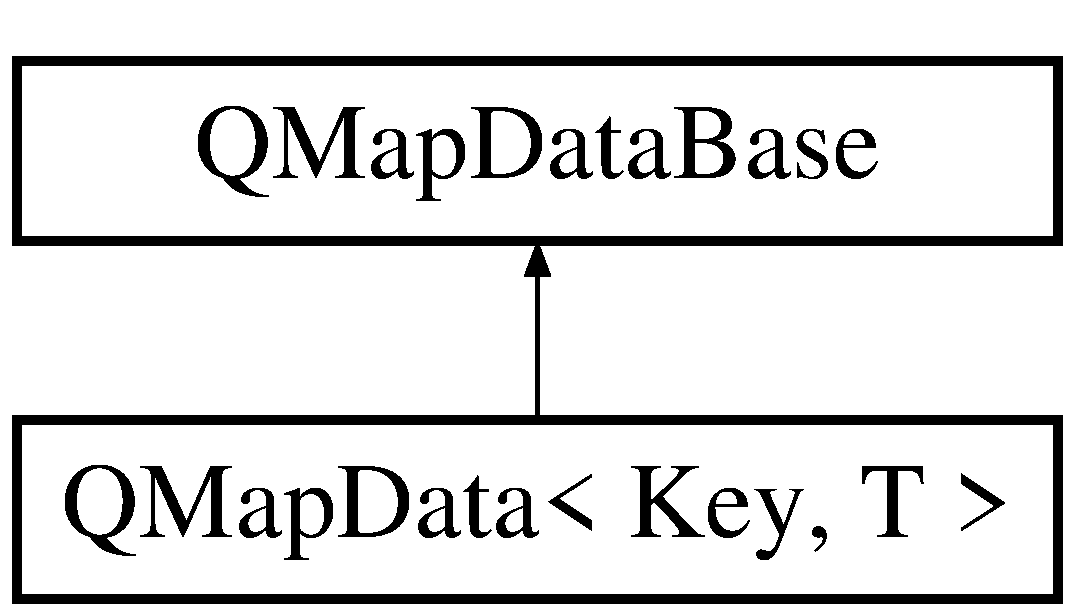
\includegraphics[height=2.000000cm]{struct_q_map_data}
\end{center}
\end{figure}
\subsection*{Public Types}
\begin{DoxyCompactItemize}
\item 
typedef \hyperlink{struct_q_map_node}{Q\+Map\+Node}$<$ Key, T $>$ \hyperlink{struct_q_map_data_a9e453de3cc687c14a51c4145bb5959c3}{Node}
\end{DoxyCompactItemize}
\subsection*{Public Member Functions}
\begin{DoxyCompactItemize}
\item 
\hyperlink{struct_q_map_data_a9e453de3cc687c14a51c4145bb5959c3}{Node} $\ast$ \hyperlink{struct_q_map_data_a124ed4fc317d52caec1cb25eb6056b61}{root} () const 
\item 
const \hyperlink{struct_q_map_data_a9e453de3cc687c14a51c4145bb5959c3}{Node} $\ast$ \hyperlink{struct_q_map_data_af4fbffb9172db96d69939747cd8ce6c2}{end} () const 
\item 
\hyperlink{struct_q_map_data_a9e453de3cc687c14a51c4145bb5959c3}{Node} $\ast$ \hyperlink{struct_q_map_data_acae8f9f98450b173a91afd1b2f902aa0}{end} ()
\item 
const \hyperlink{struct_q_map_data_a9e453de3cc687c14a51c4145bb5959c3}{Node} $\ast$ \hyperlink{struct_q_map_data_a8d1858c933d70868bf3e622ee64e34ab}{begin} () const 
\item 
\hyperlink{struct_q_map_data_a9e453de3cc687c14a51c4145bb5959c3}{Node} $\ast$ \hyperlink{struct_q_map_data_a9f336a5bc3a4e11815c0af5fb114d0da}{begin} ()
\item 
void \hyperlink{struct_q_map_data_a4b634f0177f4b09665c922560b630626}{delete\+Node} (\hyperlink{struct_q_map_data_a9e453de3cc687c14a51c4145bb5959c3}{Node} $\ast$z)
\item 
\hyperlink{struct_q_map_data_a9e453de3cc687c14a51c4145bb5959c3}{Node} $\ast$ \hyperlink{struct_q_map_data_a7a1d40fcd919b691d655912de6302706}{find\+Node} (const Key \&akey) const 
\item 
void \hyperlink{struct_q_map_data_a976acbd12ec6c68605e4cac30d57a57f}{node\+Range} (const Key \&akey, \hyperlink{struct_q_map_data_a9e453de3cc687c14a51c4145bb5959c3}{Node} $\ast$$\ast$first\+Node, \hyperlink{struct_q_map_data_a9e453de3cc687c14a51c4145bb5959c3}{Node} $\ast$$\ast$last\+Node)
\item 
\hyperlink{struct_q_map_data_a9e453de3cc687c14a51c4145bb5959c3}{Node} $\ast$ \hyperlink{struct_q_map_data_ae38d9e8096ad2175aeb788bb9ea6d5eb}{create\+Node} (const Key \&k, const T \&v, \hyperlink{struct_q_map_data_a9e453de3cc687c14a51c4145bb5959c3}{Node} $\ast$parent=0, bool left=false)
\item 
void \hyperlink{struct_q_map_data_a72c88a1d07fc5f31e989a329150ad96d}{destroy} ()
\end{DoxyCompactItemize}
\subsection*{Static Public Member Functions}
\begin{DoxyCompactItemize}
\item 
static \hyperlink{struct_q_map_data}{Q\+Map\+Data} $\ast$ \hyperlink{struct_q_map_data_ae855aaf71b9ee04929ebf852c1703074}{create} ()
\end{DoxyCompactItemize}
\subsection*{Additional Inherited Members}


\subsection{Detailed Description}
\subsubsection*{template$<$class Key, class T$>$\\*
struct Q\+Map\+Data$<$ Key, T $>$}



Definition at line 77 of file qmap.\+h.



\subsection{Member Typedef Documentation}
\index{Q\+Map\+Data@{Q\+Map\+Data}!Node@{Node}}
\index{Node@{Node}!Q\+Map\+Data@{Q\+Map\+Data}}
\subsubsection[{\texorpdfstring{Node}{Node}}]{\setlength{\rightskip}{0pt plus 5cm}template$<$class Key, class T$>$ typedef {\bf Q\+Map\+Node}$<$Key, T$>$ {\bf Q\+Map\+Data}$<$ Key, T $>$\+::{\bf Node}}\hypertarget{struct_q_map_data_a9e453de3cc687c14a51c4145bb5959c3}{}\label{struct_q_map_data_a9e453de3cc687c14a51c4145bb5959c3}


Definition at line 184 of file qmap.\+h.



\subsection{Member Function Documentation}
\index{Q\+Map\+Data@{Q\+Map\+Data}!begin@{begin}}
\index{begin@{begin}!Q\+Map\+Data@{Q\+Map\+Data}}
\subsubsection[{\texorpdfstring{begin() const }{begin() const }}]{\setlength{\rightskip}{0pt plus 5cm}template$<$class Key, class T$>$ const {\bf Node}$\ast$ {\bf Q\+Map\+Data}$<$ Key, T $>$\+::begin (
\begin{DoxyParamCaption}
{}
\end{DoxyParamCaption}
) const\hspace{0.3cm}{\ttfamily [inline]}}\hypertarget{struct_q_map_data_a8d1858c933d70868bf3e622ee64e34ab}{}\label{struct_q_map_data_a8d1858c933d70868bf3e622ee64e34ab}


Definition at line 190 of file qmap.\+h.

\index{Q\+Map\+Data@{Q\+Map\+Data}!begin@{begin}}
\index{begin@{begin}!Q\+Map\+Data@{Q\+Map\+Data}}
\subsubsection[{\texorpdfstring{begin()}{begin()}}]{\setlength{\rightskip}{0pt plus 5cm}template$<$class Key, class T$>$ {\bf Node}$\ast$ {\bf Q\+Map\+Data}$<$ Key, T $>$\+::begin (
\begin{DoxyParamCaption}
{}
\end{DoxyParamCaption}
)\hspace{0.3cm}{\ttfamily [inline]}}\hypertarget{struct_q_map_data_a9f336a5bc3a4e11815c0af5fb114d0da}{}\label{struct_q_map_data_a9f336a5bc3a4e11815c0af5fb114d0da}


Definition at line 191 of file qmap.\+h.

\index{Q\+Map\+Data@{Q\+Map\+Data}!create@{create}}
\index{create@{create}!Q\+Map\+Data@{Q\+Map\+Data}}
\subsubsection[{\texorpdfstring{create()}{create()}}]{\setlength{\rightskip}{0pt plus 5cm}template$<$class Key, class T$>$ static {\bf Q\+Map\+Data}$\ast$ {\bf Q\+Map\+Data}$<$ Key, T $>$\+::create (
\begin{DoxyParamCaption}
{}
\end{DoxyParamCaption}
)\hspace{0.3cm}{\ttfamily [inline]}, {\ttfamily [static]}}\hypertarget{struct_q_map_data_ae855aaf71b9ee04929ebf852c1703074}{}\label{struct_q_map_data_ae855aaf71b9ee04929ebf852c1703074}


Definition at line 216 of file qmap.\+h.

\index{Q\+Map\+Data@{Q\+Map\+Data}!create\+Node@{create\+Node}}
\index{create\+Node@{create\+Node}!Q\+Map\+Data@{Q\+Map\+Data}}
\subsubsection[{\texorpdfstring{create\+Node(const Key \&k, const T \&v, Node $\ast$parent=0, bool left=false)}{createNode(const Key &k, const T &v, Node *parent=0, bool left=false)}}]{\setlength{\rightskip}{0pt plus 5cm}template$<$class Key, class T$>$ {\bf Node}$\ast$ {\bf Q\+Map\+Data}$<$ Key, T $>$\+::create\+Node (
\begin{DoxyParamCaption}
\item[{const Key \&}]{k, }
\item[{const T \&}]{v, }
\item[{{\bf Node} $\ast$}]{parent = {\ttfamily 0}, }
\item[{bool}]{left = {\ttfamily false}}
\end{DoxyParamCaption}
)\hspace{0.3cm}{\ttfamily [inline]}}\hypertarget{struct_q_map_data_ae38d9e8096ad2175aeb788bb9ea6d5eb}{}\label{struct_q_map_data_ae38d9e8096ad2175aeb788bb9ea6d5eb}


Definition at line 197 of file qmap.\+h.

\index{Q\+Map\+Data@{Q\+Map\+Data}!delete\+Node@{delete\+Node}}
\index{delete\+Node@{delete\+Node}!Q\+Map\+Data@{Q\+Map\+Data}}
\subsubsection[{\texorpdfstring{delete\+Node(\+Node $\ast$z)}{deleteNode(Node *z)}}]{\setlength{\rightskip}{0pt plus 5cm}template$<$class Key , class T $>$ void {\bf Q\+Map\+Data}$<$ Key, T $>$\+::delete\+Node (
\begin{DoxyParamCaption}
\item[{{\bf Node} $\ast$}]{z}
\end{DoxyParamCaption}
)}\hypertarget{struct_q_map_data_a4b634f0177f4b09665c922560b630626}{}\label{struct_q_map_data_a4b634f0177f4b09665c922560b630626}


Definition at line 274 of file qmap.\+h.

\index{Q\+Map\+Data@{Q\+Map\+Data}!destroy@{destroy}}
\index{destroy@{destroy}!Q\+Map\+Data@{Q\+Map\+Data}}
\subsubsection[{\texorpdfstring{destroy()}{destroy()}}]{\setlength{\rightskip}{0pt plus 5cm}template$<$class Key, class T$>$ void {\bf Q\+Map\+Data}$<$ Key, T $>$\+::destroy (
\begin{DoxyParamCaption}
{}
\end{DoxyParamCaption}
)\hspace{0.3cm}{\ttfamily [inline]}}\hypertarget{struct_q_map_data_a72c88a1d07fc5f31e989a329150ad96d}{}\label{struct_q_map_data_a72c88a1d07fc5f31e989a329150ad96d}


Definition at line 220 of file qmap.\+h.

\index{Q\+Map\+Data@{Q\+Map\+Data}!end@{end}}
\index{end@{end}!Q\+Map\+Data@{Q\+Map\+Data}}
\subsubsection[{\texorpdfstring{end() const }{end() const }}]{\setlength{\rightskip}{0pt plus 5cm}template$<$class Key, class T$>$ const {\bf Node}$\ast$ {\bf Q\+Map\+Data}$<$ Key, T $>$\+::end (
\begin{DoxyParamCaption}
{}
\end{DoxyParamCaption}
) const\hspace{0.3cm}{\ttfamily [inline]}}\hypertarget{struct_q_map_data_af4fbffb9172db96d69939747cd8ce6c2}{}\label{struct_q_map_data_af4fbffb9172db96d69939747cd8ce6c2}


Definition at line 188 of file qmap.\+h.

\index{Q\+Map\+Data@{Q\+Map\+Data}!end@{end}}
\index{end@{end}!Q\+Map\+Data@{Q\+Map\+Data}}
\subsubsection[{\texorpdfstring{end()}{end()}}]{\setlength{\rightskip}{0pt plus 5cm}template$<$class Key, class T$>$ {\bf Node}$\ast$ {\bf Q\+Map\+Data}$<$ Key, T $>$\+::end (
\begin{DoxyParamCaption}
{}
\end{DoxyParamCaption}
)\hspace{0.3cm}{\ttfamily [inline]}}\hypertarget{struct_q_map_data_acae8f9f98450b173a91afd1b2f902aa0}{}\label{struct_q_map_data_acae8f9f98450b173a91afd1b2f902aa0}


Definition at line 189 of file qmap.\+h.

\index{Q\+Map\+Data@{Q\+Map\+Data}!find\+Node@{find\+Node}}
\index{find\+Node@{find\+Node}!Q\+Map\+Data@{Q\+Map\+Data}}
\subsubsection[{\texorpdfstring{find\+Node(const Key \&akey) const }{findNode(const Key &akey) const }}]{\setlength{\rightskip}{0pt plus 5cm}template$<$class Key, class T $>$ {\bf Q\+Map\+Node}$<$ Key, T $>$ $\ast$ {\bf Q\+Map\+Data}$<$ Key, T $>$\+::find\+Node (
\begin{DoxyParamCaption}
\item[{const Key \&}]{akey}
\end{DoxyParamCaption}
) const}\hypertarget{struct_q_map_data_a7a1d40fcd919b691d655912de6302706}{}\label{struct_q_map_data_a7a1d40fcd919b691d655912de6302706}


Definition at line 284 of file qmap.\+h.

\index{Q\+Map\+Data@{Q\+Map\+Data}!node\+Range@{node\+Range}}
\index{node\+Range@{node\+Range}!Q\+Map\+Data@{Q\+Map\+Data}}
\subsubsection[{\texorpdfstring{node\+Range(const Key \&akey, Node $\ast$$\ast$first\+Node, Node $\ast$$\ast$last\+Node)}{nodeRange(const Key &akey, Node **firstNode, Node **lastNode)}}]{\setlength{\rightskip}{0pt plus 5cm}template$<$class Key, class T $>$ void {\bf Q\+Map\+Data}$<$ Key, T $>$\+::node\+Range (
\begin{DoxyParamCaption}
\item[{const Key \&}]{akey, }
\item[{{\bf Node} $\ast$$\ast$}]{first\+Node, }
\item[{{\bf Node} $\ast$$\ast$}]{last\+Node}
\end{DoxyParamCaption}
)}\hypertarget{struct_q_map_data_a976acbd12ec6c68605e4cac30d57a57f}{}\label{struct_q_map_data_a976acbd12ec6c68605e4cac30d57a57f}


Definition at line 296 of file qmap.\+h.

\index{Q\+Map\+Data@{Q\+Map\+Data}!root@{root}}
\index{root@{root}!Q\+Map\+Data@{Q\+Map\+Data}}
\subsubsection[{\texorpdfstring{root() const }{root() const }}]{\setlength{\rightskip}{0pt plus 5cm}template$<$class Key, class T$>$ {\bf Node}$\ast$ {\bf Q\+Map\+Data}$<$ Key, T $>$\+::root (
\begin{DoxyParamCaption}
{}
\end{DoxyParamCaption}
) const\hspace{0.3cm}{\ttfamily [inline]}}\hypertarget{struct_q_map_data_a124ed4fc317d52caec1cb25eb6056b61}{}\label{struct_q_map_data_a124ed4fc317d52caec1cb25eb6056b61}


Definition at line 186 of file qmap.\+h.



The documentation for this struct was generated from the following file\+:\begin{DoxyCompactItemize}
\item 
docs/extra-\/files/\hyperlink{qmap_8h}{qmap.\+h}\end{DoxyCompactItemize}

\hypertarget{struct_q_map_data_base}{}\section{Q\+Map\+Data\+Base Struct Reference}
\label{struct_q_map_data_base}\index{Q\+Map\+Data\+Base@{Q\+Map\+Data\+Base}}


{\ttfamily \#include $<$qmap.\+h$>$}

Inheritance diagram for Q\+Map\+Data\+Base\+:\begin{figure}[H]
\begin{center}
\leavevmode
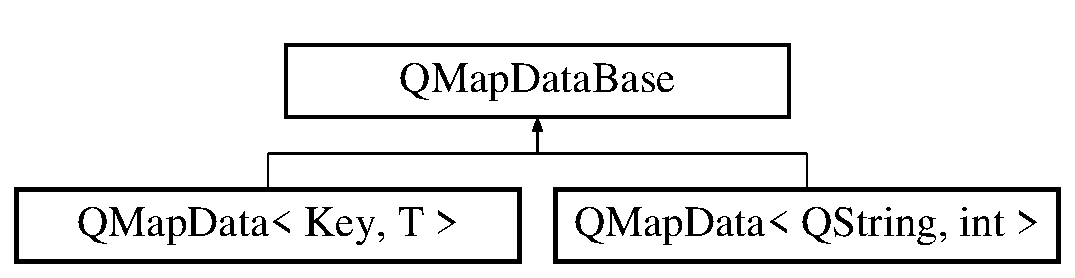
\includegraphics[height=2.000000cm]{struct_q_map_data_base}
\end{center}
\end{figure}
\subsection*{Public Member Functions}
\begin{DoxyCompactItemize}
\item 
void \hyperlink{struct_q_map_data_base_affa79abf5995456a9cbf12a2306c8041}{rotate\+Left} (\hyperlink{struct_q_map_node_base}{Q\+Map\+Node\+Base} $\ast$x)
\item 
void \hyperlink{struct_q_map_data_base_a33a1fdcca7a3ddd4406e72cbeb71cf05}{rotate\+Right} (\hyperlink{struct_q_map_node_base}{Q\+Map\+Node\+Base} $\ast$x)
\item 
void \hyperlink{struct_q_map_data_base_a305bcd1ed005eed9f0e3a1478b7a022b}{rebalance} (\hyperlink{struct_q_map_node_base}{Q\+Map\+Node\+Base} $\ast$x)
\item 
void \hyperlink{struct_q_map_data_base_a141a896a0c94c46f9fcaa25ba8ba8bad}{free\+Node\+And\+Rebalance} (\hyperlink{struct_q_map_node_base}{Q\+Map\+Node\+Base} $\ast$z)
\item 
void \hyperlink{struct_q_map_data_base_ab24efe6e9bca4df9fba86b1b7382f0c0}{recalc\+Most\+Left\+Node} ()
\item 
\hyperlink{struct_q_map_node_base}{Q\+Map\+Node\+Base} $\ast$ \hyperlink{struct_q_map_data_base_ae681f8e156f10fef6238773ad833dc63}{create\+Node} (int \hyperlink{struct_q_map_data_base_a61b8b87aa9f55d8380f67b5b9f4bc786}{size}, int alignment, \hyperlink{struct_q_map_node_base}{Q\+Map\+Node\+Base} $\ast$parent, bool left)
\item 
void \hyperlink{struct_q_map_data_base_aa1e11406977158087b85d06b61fd64f8}{free\+Tree} (\hyperlink{struct_q_map_node_base}{Q\+Map\+Node\+Base} $\ast$root, int alignment)
\end{DoxyCompactItemize}
\subsection*{Static Public Member Functions}
\begin{DoxyCompactItemize}
\item 
static \hyperlink{struct_q_map_data_base}{Q\+Map\+Data\+Base} $\ast$ \hyperlink{struct_q_map_data_base_ab73fd1ef8a7fc94981f175cc8c961498}{create\+Data} ()
\item 
static void \hyperlink{struct_q_map_data_base_a0d6f53d631ecc76af76e79ceb9557e4a}{free\+Data} (\hyperlink{struct_q_map_data_base}{Q\+Map\+Data\+Base} $\ast$d)
\end{DoxyCompactItemize}
\subsection*{Public Attributes}
\begin{DoxyCompactItemize}
\item 
Qt\+Private\+::\+Ref\+Count \hyperlink{struct_q_map_data_base_ab3039892c5c68597eeb0746c26459d42}{ref}
\item 
int \hyperlink{struct_q_map_data_base_a61b8b87aa9f55d8380f67b5b9f4bc786}{size}
\item 
\hyperlink{struct_q_map_node_base}{Q\+Map\+Node\+Base} \hyperlink{struct_q_map_data_base_a11102879d6fba5de5d44220294c4ac03}{header}
\item 
\hyperlink{struct_q_map_node_base}{Q\+Map\+Node\+Base} $\ast$ \hyperlink{struct_q_map_data_base_a836e3d0106d5ae7a9bb5f61ab06ee7ef}{most\+Left\+Node}
\end{DoxyCompactItemize}
\subsection*{Static Public Attributes}
\begin{DoxyCompactItemize}
\item 
static const \hyperlink{struct_q_map_data_base}{Q\+Map\+Data\+Base} \hyperlink{struct_q_map_data_base_ac279e752e04494bb619c9d26763d2eb7}{shared\+\_\+null} = \{ Q\+\_\+\+R\+E\+F\+C\+O\+U\+N\+T\+\_\+\+I\+N\+I\+T\+I\+A\+L\+I\+Z\+E\+\_\+\+S\+T\+A\+T\+IC, 0, \{ 0, 0, 0 \}, 0 \}
\end{DoxyCompactItemize}


\subsection{Detailed Description}


Definition at line 159 of file qmap.\+h.



\subsection{Member Function Documentation}
\index{Q\+Map\+Data\+Base@{Q\+Map\+Data\+Base}!create\+Data@{create\+Data}}
\index{create\+Data@{create\+Data}!Q\+Map\+Data\+Base@{Q\+Map\+Data\+Base}}
\subsubsection[{\texorpdfstring{create\+Data()}{createData()}}]{\setlength{\rightskip}{0pt plus 5cm}{\bf Q\+Map\+Data\+Base} $\ast$ Q\+Map\+Data\+Base\+::create\+Data (
\begin{DoxyParamCaption}
{}
\end{DoxyParamCaption}
)\hspace{0.3cm}{\ttfamily [static]}}\hypertarget{struct_q_map_data_base_ab73fd1ef8a7fc94981f175cc8c961498}{}\label{struct_q_map_data_base_ab73fd1ef8a7fc94981f175cc8c961498}


Definition at line 352 of file qmap.\+cpp.

\index{Q\+Map\+Data\+Base@{Q\+Map\+Data\+Base}!create\+Node@{create\+Node}}
\index{create\+Node@{create\+Node}!Q\+Map\+Data\+Base@{Q\+Map\+Data\+Base}}
\subsubsection[{\texorpdfstring{create\+Node(int size, int alignment, Q\+Map\+Node\+Base $\ast$parent, bool left)}{createNode(int size, int alignment, QMapNodeBase *parent, bool left)}}]{\setlength{\rightskip}{0pt plus 5cm}{\bf Q\+Map\+Node\+Base} $\ast$ Q\+Map\+Data\+Base\+::create\+Node (
\begin{DoxyParamCaption}
\item[{int}]{size, }
\item[{int}]{alignment, }
\item[{{\bf Q\+Map\+Node\+Base} $\ast$}]{parent, }
\item[{bool}]{left}
\end{DoxyParamCaption}
)}\hypertarget{struct_q_map_data_base_ae681f8e156f10fef6238773ad833dc63}{}\label{struct_q_map_data_base_ae681f8e156f10fef6238773ad833dc63}


Definition at line 321 of file qmap.\+cpp.

\index{Q\+Map\+Data\+Base@{Q\+Map\+Data\+Base}!free\+Data@{free\+Data}}
\index{free\+Data@{free\+Data}!Q\+Map\+Data\+Base@{Q\+Map\+Data\+Base}}
\subsubsection[{\texorpdfstring{free\+Data(\+Q\+Map\+Data\+Base $\ast$d)}{freeData(QMapDataBase *d)}}]{\setlength{\rightskip}{0pt plus 5cm}void Q\+Map\+Data\+Base\+::free\+Data (
\begin{DoxyParamCaption}
\item[{{\bf Q\+Map\+Data\+Base} $\ast$}]{d}
\end{DoxyParamCaption}
)\hspace{0.3cm}{\ttfamily [static]}}\hypertarget{struct_q_map_data_base_a0d6f53d631ecc76af76e79ceb9557e4a}{}\label{struct_q_map_data_base_a0d6f53d631ecc76af76e79ceb9557e4a}


Definition at line 367 of file qmap.\+cpp.

\index{Q\+Map\+Data\+Base@{Q\+Map\+Data\+Base}!free\+Node\+And\+Rebalance@{free\+Node\+And\+Rebalance}}
\index{free\+Node\+And\+Rebalance@{free\+Node\+And\+Rebalance}!Q\+Map\+Data\+Base@{Q\+Map\+Data\+Base}}
\subsubsection[{\texorpdfstring{free\+Node\+And\+Rebalance(\+Q\+Map\+Node\+Base $\ast$z)}{freeNodeAndRebalance(QMapNodeBase *z)}}]{\setlength{\rightskip}{0pt plus 5cm}void Q\+Map\+Data\+Base\+::free\+Node\+And\+Rebalance (
\begin{DoxyParamCaption}
\item[{{\bf Q\+Map\+Node\+Base} $\ast$}]{z}
\end{DoxyParamCaption}
)}\hypertarget{struct_q_map_data_base_a141a896a0c94c46f9fcaa25ba8ba8bad}{}\label{struct_q_map_data_base_a141a896a0c94c46f9fcaa25ba8ba8bad}


Definition at line 164 of file qmap.\+cpp.

\index{Q\+Map\+Data\+Base@{Q\+Map\+Data\+Base}!free\+Tree@{free\+Tree}}
\index{free\+Tree@{free\+Tree}!Q\+Map\+Data\+Base@{Q\+Map\+Data\+Base}}
\subsubsection[{\texorpdfstring{free\+Tree(\+Q\+Map\+Node\+Base $\ast$root, int alignment)}{freeTree(QMapNodeBase *root, int alignment)}}]{\setlength{\rightskip}{0pt plus 5cm}void Q\+Map\+Data\+Base\+::free\+Tree (
\begin{DoxyParamCaption}
\item[{{\bf Q\+Map\+Node\+Base} $\ast$}]{root, }
\item[{int}]{alignment}
\end{DoxyParamCaption}
)}\hypertarget{struct_q_map_data_base_aa1e11406977158087b85d06b61fd64f8}{}\label{struct_q_map_data_base_aa1e11406977158087b85d06b61fd64f8}


Definition at line 343 of file qmap.\+cpp.

\index{Q\+Map\+Data\+Base@{Q\+Map\+Data\+Base}!rebalance@{rebalance}}
\index{rebalance@{rebalance}!Q\+Map\+Data\+Base@{Q\+Map\+Data\+Base}}
\subsubsection[{\texorpdfstring{rebalance(\+Q\+Map\+Node\+Base $\ast$x)}{rebalance(QMapNodeBase *x)}}]{\setlength{\rightskip}{0pt plus 5cm}void Q\+Map\+Data\+Base\+::rebalance (
\begin{DoxyParamCaption}
\item[{{\bf Q\+Map\+Node\+Base} $\ast$}]{x}
\end{DoxyParamCaption}
)}\hypertarget{struct_q_map_data_base_a305bcd1ed005eed9f0e3a1478b7a022b}{}\label{struct_q_map_data_base_a305bcd1ed005eed9f0e3a1478b7a022b}


Definition at line 122 of file qmap.\+cpp.

\index{Q\+Map\+Data\+Base@{Q\+Map\+Data\+Base}!recalc\+Most\+Left\+Node@{recalc\+Most\+Left\+Node}}
\index{recalc\+Most\+Left\+Node@{recalc\+Most\+Left\+Node}!Q\+Map\+Data\+Base@{Q\+Map\+Data\+Base}}
\subsubsection[{\texorpdfstring{recalc\+Most\+Left\+Node()}{recalcMostLeftNode()}}]{\setlength{\rightskip}{0pt plus 5cm}void Q\+Map\+Data\+Base\+::recalc\+Most\+Left\+Node (
\begin{DoxyParamCaption}
{}
\end{DoxyParamCaption}
)}\hypertarget{struct_q_map_data_base_ab24efe6e9bca4df9fba86b1b7382f0c0}{}\label{struct_q_map_data_base_ab24efe6e9bca4df9fba86b1b7382f0c0}


Definition at line 291 of file qmap.\+cpp.

\index{Q\+Map\+Data\+Base@{Q\+Map\+Data\+Base}!rotate\+Left@{rotate\+Left}}
\index{rotate\+Left@{rotate\+Left}!Q\+Map\+Data\+Base@{Q\+Map\+Data\+Base}}
\subsubsection[{\texorpdfstring{rotate\+Left(\+Q\+Map\+Node\+Base $\ast$x)}{rotateLeft(QMapNodeBase *x)}}]{\setlength{\rightskip}{0pt plus 5cm}void Q\+Map\+Data\+Base\+::rotate\+Left (
\begin{DoxyParamCaption}
\item[{{\bf Q\+Map\+Node\+Base} $\ast$}]{x}
\end{DoxyParamCaption}
)}\hypertarget{struct_q_map_data_base_affa79abf5995456a9cbf12a2306c8041}{}\label{struct_q_map_data_base_affa79abf5995456a9cbf12a2306c8041}


Definition at line 84 of file qmap.\+cpp.

\index{Q\+Map\+Data\+Base@{Q\+Map\+Data\+Base}!rotate\+Right@{rotate\+Right}}
\index{rotate\+Right@{rotate\+Right}!Q\+Map\+Data\+Base@{Q\+Map\+Data\+Base}}
\subsubsection[{\texorpdfstring{rotate\+Right(\+Q\+Map\+Node\+Base $\ast$x)}{rotateRight(QMapNodeBase *x)}}]{\setlength{\rightskip}{0pt plus 5cm}void Q\+Map\+Data\+Base\+::rotate\+Right (
\begin{DoxyParamCaption}
\item[{{\bf Q\+Map\+Node\+Base} $\ast$}]{x}
\end{DoxyParamCaption}
)}\hypertarget{struct_q_map_data_base_a33a1fdcca7a3ddd4406e72cbeb71cf05}{}\label{struct_q_map_data_base_a33a1fdcca7a3ddd4406e72cbeb71cf05}


Definition at line 103 of file qmap.\+cpp.



\subsection{Member Data Documentation}
\index{Q\+Map\+Data\+Base@{Q\+Map\+Data\+Base}!header@{header}}
\index{header@{header}!Q\+Map\+Data\+Base@{Q\+Map\+Data\+Base}}
\subsubsection[{\texorpdfstring{header}{header}}]{\setlength{\rightskip}{0pt plus 5cm}{\bf Q\+Map\+Node\+Base} Q\+Map\+Data\+Base\+::header}\hypertarget{struct_q_map_data_base_a11102879d6fba5de5d44220294c4ac03}{}\label{struct_q_map_data_base_a11102879d6fba5de5d44220294c4ac03}


Definition at line 163 of file qmap.\+h.

\index{Q\+Map\+Data\+Base@{Q\+Map\+Data\+Base}!most\+Left\+Node@{most\+Left\+Node}}
\index{most\+Left\+Node@{most\+Left\+Node}!Q\+Map\+Data\+Base@{Q\+Map\+Data\+Base}}
\subsubsection[{\texorpdfstring{most\+Left\+Node}{mostLeftNode}}]{\setlength{\rightskip}{0pt plus 5cm}{\bf Q\+Map\+Node\+Base}$\ast$ Q\+Map\+Data\+Base\+::most\+Left\+Node}\hypertarget{struct_q_map_data_base_a836e3d0106d5ae7a9bb5f61ab06ee7ef}{}\label{struct_q_map_data_base_a836e3d0106d5ae7a9bb5f61ab06ee7ef}


Definition at line 164 of file qmap.\+h.

\index{Q\+Map\+Data\+Base@{Q\+Map\+Data\+Base}!ref@{ref}}
\index{ref@{ref}!Q\+Map\+Data\+Base@{Q\+Map\+Data\+Base}}
\subsubsection[{\texorpdfstring{ref}{ref}}]{\setlength{\rightskip}{0pt plus 5cm}Qt\+Private\+::\+Ref\+Count Q\+Map\+Data\+Base\+::ref}\hypertarget{struct_q_map_data_base_ab3039892c5c68597eeb0746c26459d42}{}\label{struct_q_map_data_base_ab3039892c5c68597eeb0746c26459d42}


Definition at line 161 of file qmap.\+h.

\index{Q\+Map\+Data\+Base@{Q\+Map\+Data\+Base}!shared\+\_\+null@{shared\+\_\+null}}
\index{shared\+\_\+null@{shared\+\_\+null}!Q\+Map\+Data\+Base@{Q\+Map\+Data\+Base}}
\subsubsection[{\texorpdfstring{shared\+\_\+null}{shared_null}}]{\setlength{\rightskip}{0pt plus 5cm}Q\+T\+\_\+\+B\+E\+G\+I\+N\+\_\+\+N\+A\+M\+E\+S\+P\+A\+CE const {\bf Q\+Map\+Data\+Base} Q\+Map\+Data\+Base\+::shared\+\_\+null = \{ Q\+\_\+\+R\+E\+F\+C\+O\+U\+N\+T\+\_\+\+I\+N\+I\+T\+I\+A\+L\+I\+Z\+E\+\_\+\+S\+T\+A\+T\+IC, 0, \{ 0, 0, 0 \}, 0 \}\hspace{0.3cm}{\ttfamily [static]}}\hypertarget{struct_q_map_data_base_ac279e752e04494bb619c9d26763d2eb7}{}\label{struct_q_map_data_base_ac279e752e04494bb619c9d26763d2eb7}


Definition at line 175 of file qmap.\+h.

\index{Q\+Map\+Data\+Base@{Q\+Map\+Data\+Base}!size@{size}}
\index{size@{size}!Q\+Map\+Data\+Base@{Q\+Map\+Data\+Base}}
\subsubsection[{\texorpdfstring{size}{size}}]{\setlength{\rightskip}{0pt plus 5cm}int Q\+Map\+Data\+Base\+::size}\hypertarget{struct_q_map_data_base_a61b8b87aa9f55d8380f67b5b9f4bc786}{}\label{struct_q_map_data_base_a61b8b87aa9f55d8380f67b5b9f4bc786}


Definition at line 162 of file qmap.\+h.



The documentation for this struct was generated from the following files\+:\begin{DoxyCompactItemize}
\item 
docs/extra-\/files/\hyperlink{qmap_8h}{qmap.\+h}\item 
docs/extra-\/files/\hyperlink{qmap_8cpp}{qmap.\+cpp}\end{DoxyCompactItemize}

\hypertarget{struct_q_map_node}{}\section{Q\+Map\+Node$<$ Key, T $>$ Struct Template Reference}
\label{struct_q_map_node}\index{Q\+Map\+Node$<$ Key, T $>$@{Q\+Map\+Node$<$ Key, T $>$}}


{\ttfamily \#include $<$qmap.\+h$>$}

Inheritance diagram for Q\+Map\+Node$<$ Key, T $>$\+:\begin{figure}[H]
\begin{center}
\leavevmode
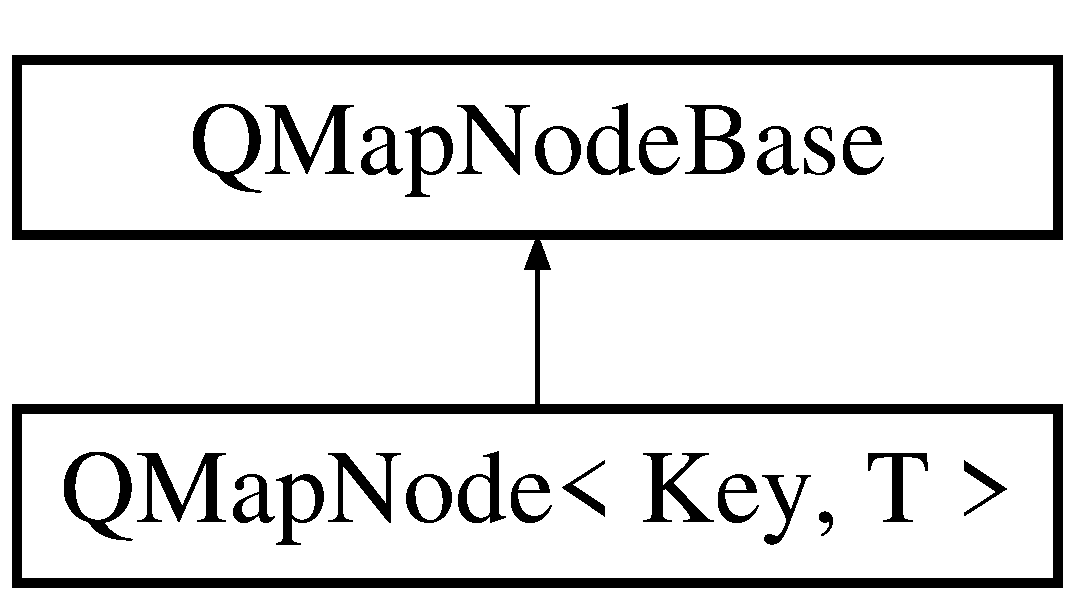
\includegraphics[height=2.000000cm]{struct_q_map_node}
\end{center}
\end{figure}
\subsection*{Public Member Functions}
\begin{DoxyCompactItemize}
\item 
\hyperlink{struct_q_map_node}{Q\+Map\+Node} $\ast$ \hyperlink{struct_q_map_node_a9bac36e9a52f89639bd2fa7f4839650d}{left\+Node} () const 
\item 
\hyperlink{struct_q_map_node}{Q\+Map\+Node} $\ast$ \hyperlink{struct_q_map_node_a94e6d3149e83ad24beaaf45cc16e800c}{right\+Node} () const 
\item 
const \hyperlink{struct_q_map_node}{Q\+Map\+Node} $\ast$ \hyperlink{struct_q_map_node_ae2b84505a38a7bd58e843021eceb679d}{next\+Node} () const 
\item 
const \hyperlink{struct_q_map_node}{Q\+Map\+Node} $\ast$ \hyperlink{struct_q_map_node_a8998806963e7a7180fbb021503c0e5c5}{previous\+Node} () const 
\item 
\hyperlink{struct_q_map_node}{Q\+Map\+Node} $\ast$ \hyperlink{struct_q_map_node_a63314461289c232d3d8b813b3431a95d}{next\+Node} ()
\item 
\hyperlink{struct_q_map_node}{Q\+Map\+Node} $\ast$ \hyperlink{struct_q_map_node_ac76d623654ec393538172c95e4d7f4f9}{previous\+Node} ()
\item 
\hyperlink{struct_q_map_node}{Q\+Map\+Node}$<$ Key, T $>$ $\ast$ \hyperlink{struct_q_map_node_af28a6a3ca05bb30fa33defd63d7bb237}{copy} (\hyperlink{struct_q_map_data}{Q\+Map\+Data}$<$ Key, T $>$ $\ast$d) const 
\item 
void \hyperlink{struct_q_map_node_a4dcf5b5c4bb4d8df0805abf6de104dea}{destroy\+Sub\+Tree} ()
\item 
\hyperlink{struct_q_map_node}{Q\+Map\+Node}$<$ Key, T $>$ $\ast$ \hyperlink{struct_q_map_node_a54614b1c04773d2380382fe0dcee38e7}{lower\+Bound} (const Key \&\hyperlink{struct_q_map_node_a6300e95158f21d89fcd4059fb75fb3d6}{key})
\item 
\hyperlink{struct_q_map_node}{Q\+Map\+Node}$<$ Key, T $>$ $\ast$ \hyperlink{struct_q_map_node_ad80318241539f08d081275f1a757cff3}{upper\+Bound} (const Key \&\hyperlink{struct_q_map_node_a6300e95158f21d89fcd4059fb75fb3d6}{key})
\end{DoxyCompactItemize}
\subsection*{Public Attributes}
\begin{DoxyCompactItemize}
\item 
Key \hyperlink{struct_q_map_node_a6300e95158f21d89fcd4059fb75fb3d6}{key}
\item 
T \hyperlink{struct_q_map_node_a872bc4a284250baed9e3dc22b8e39692}{value}
\end{DoxyCompactItemize}
\subsection*{Additional Inherited Members}


\subsection{Detailed Description}
\subsubsection*{template$<$class Key, class T$>$\\*
struct Q\+Map\+Node$<$ Key, T $>$}



Definition at line 100 of file qmap.\+h.



\subsection{Member Function Documentation}
\index{Q\+Map\+Node@{Q\+Map\+Node}!copy@{copy}}
\index{copy@{copy}!Q\+Map\+Node@{Q\+Map\+Node}}
\subsubsection[{\texorpdfstring{copy(\+Q\+Map\+Data$<$ Key, T $>$ $\ast$d) const }{copy(QMapData< Key, T > *d) const }}]{\setlength{\rightskip}{0pt plus 5cm}template$<$class Key , class T $>$ {\bf Q\+Map\+Node}$<$ Key, T $>$ $\ast$ {\bf Q\+Map\+Node}$<$ Key, T $>$\+::copy (
\begin{DoxyParamCaption}
\item[{{\bf Q\+Map\+Data}$<$ Key, T $>$ $\ast$}]{d}
\end{DoxyParamCaption}
) const}\hypertarget{struct_q_map_node_af28a6a3ca05bb30fa33defd63d7bb237}{}\label{struct_q_map_node_af28a6a3ca05bb30fa33defd63d7bb237}


Definition at line 230 of file qmap.\+h.

\index{Q\+Map\+Node@{Q\+Map\+Node}!destroy\+Sub\+Tree@{destroy\+Sub\+Tree}}
\index{destroy\+Sub\+Tree@{destroy\+Sub\+Tree}!Q\+Map\+Node@{Q\+Map\+Node}}
\subsubsection[{\texorpdfstring{destroy\+Sub\+Tree()}{destroySubTree()}}]{\setlength{\rightskip}{0pt plus 5cm}template$<$class Key , class T $>$ void {\bf Q\+Map\+Node}$<$ Key, T $>$\+::destroy\+Sub\+Tree (
\begin{DoxyParamCaption}
{}
\end{DoxyParamCaption}
)}\hypertarget{struct_q_map_node_a4dcf5b5c4bb4d8df0805abf6de104dea}{}\label{struct_q_map_node_a4dcf5b5c4bb4d8df0805abf6de104dea}


Definition at line 255 of file qmap.\+h.

\index{Q\+Map\+Node@{Q\+Map\+Node}!left\+Node@{left\+Node}}
\index{left\+Node@{left\+Node}!Q\+Map\+Node@{Q\+Map\+Node}}
\subsubsection[{\texorpdfstring{left\+Node() const }{leftNode() const }}]{\setlength{\rightskip}{0pt plus 5cm}template$<$class Key, class T$>$ {\bf Q\+Map\+Node}$\ast$ {\bf Q\+Map\+Node}$<$ Key, T $>$\+::left\+Node (
\begin{DoxyParamCaption}
{}
\end{DoxyParamCaption}
) const\hspace{0.3cm}{\ttfamily [inline]}}\hypertarget{struct_q_map_node_a9bac36e9a52f89639bd2fa7f4839650d}{}\label{struct_q_map_node_a9bac36e9a52f89639bd2fa7f4839650d}


Definition at line 105 of file qmap.\+h.

\index{Q\+Map\+Node@{Q\+Map\+Node}!lower\+Bound@{lower\+Bound}}
\index{lower\+Bound@{lower\+Bound}!Q\+Map\+Node@{Q\+Map\+Node}}
\subsubsection[{\texorpdfstring{lower\+Bound(const Key \&key)}{lowerBound(const Key &key)}}]{\setlength{\rightskip}{0pt plus 5cm}template$<$class Key , class T $>$ {\bf Q\+Map\+Node}$<$ Key, T $>$ $\ast$ {\bf Q\+Map\+Node}$<$ Key, T $>$\+::lower\+Bound (
\begin{DoxyParamCaption}
\item[{const Key \&}]{key}
\end{DoxyParamCaption}
)\hspace{0.3cm}{\ttfamily [inline]}}\hypertarget{struct_q_map_node_a54614b1c04773d2380382fe0dcee38e7}{}\label{struct_q_map_node_a54614b1c04773d2380382fe0dcee38e7}


Definition at line 126 of file qmap.\+h.

\index{Q\+Map\+Node@{Q\+Map\+Node}!next\+Node@{next\+Node}}
\index{next\+Node@{next\+Node}!Q\+Map\+Node@{Q\+Map\+Node}}
\subsubsection[{\texorpdfstring{next\+Node() const }{nextNode() const }}]{\setlength{\rightskip}{0pt plus 5cm}template$<$class Key, class T$>$ const {\bf Q\+Map\+Node}$\ast$ {\bf Q\+Map\+Node}$<$ Key, T $>$\+::next\+Node (
\begin{DoxyParamCaption}
{}
\end{DoxyParamCaption}
) const\hspace{0.3cm}{\ttfamily [inline]}}\hypertarget{struct_q_map_node_ae2b84505a38a7bd58e843021eceb679d}{}\label{struct_q_map_node_ae2b84505a38a7bd58e843021eceb679d}


Definition at line 108 of file qmap.\+h.

\index{Q\+Map\+Node@{Q\+Map\+Node}!next\+Node@{next\+Node}}
\index{next\+Node@{next\+Node}!Q\+Map\+Node@{Q\+Map\+Node}}
\subsubsection[{\texorpdfstring{next\+Node()}{nextNode()}}]{\setlength{\rightskip}{0pt plus 5cm}template$<$class Key, class T$>$ {\bf Q\+Map\+Node}$\ast$ {\bf Q\+Map\+Node}$<$ Key, T $>$\+::next\+Node (
\begin{DoxyParamCaption}
{}
\end{DoxyParamCaption}
)\hspace{0.3cm}{\ttfamily [inline]}}\hypertarget{struct_q_map_node_a63314461289c232d3d8b813b3431a95d}{}\label{struct_q_map_node_a63314461289c232d3d8b813b3431a95d}


Definition at line 110 of file qmap.\+h.

\index{Q\+Map\+Node@{Q\+Map\+Node}!previous\+Node@{previous\+Node}}
\index{previous\+Node@{previous\+Node}!Q\+Map\+Node@{Q\+Map\+Node}}
\subsubsection[{\texorpdfstring{previous\+Node() const }{previousNode() const }}]{\setlength{\rightskip}{0pt plus 5cm}template$<$class Key, class T$>$ const {\bf Q\+Map\+Node}$\ast$ {\bf Q\+Map\+Node}$<$ Key, T $>$\+::previous\+Node (
\begin{DoxyParamCaption}
{}
\end{DoxyParamCaption}
) const\hspace{0.3cm}{\ttfamily [inline]}}\hypertarget{struct_q_map_node_a8998806963e7a7180fbb021503c0e5c5}{}\label{struct_q_map_node_a8998806963e7a7180fbb021503c0e5c5}


Definition at line 109 of file qmap.\+h.

\index{Q\+Map\+Node@{Q\+Map\+Node}!previous\+Node@{previous\+Node}}
\index{previous\+Node@{previous\+Node}!Q\+Map\+Node@{Q\+Map\+Node}}
\subsubsection[{\texorpdfstring{previous\+Node()}{previousNode()}}]{\setlength{\rightskip}{0pt plus 5cm}template$<$class Key, class T$>$ {\bf Q\+Map\+Node}$\ast$ {\bf Q\+Map\+Node}$<$ Key, T $>$\+::previous\+Node (
\begin{DoxyParamCaption}
{}
\end{DoxyParamCaption}
)\hspace{0.3cm}{\ttfamily [inline]}}\hypertarget{struct_q_map_node_ac76d623654ec393538172c95e4d7f4f9}{}\label{struct_q_map_node_ac76d623654ec393538172c95e4d7f4f9}


Definition at line 111 of file qmap.\+h.

\index{Q\+Map\+Node@{Q\+Map\+Node}!right\+Node@{right\+Node}}
\index{right\+Node@{right\+Node}!Q\+Map\+Node@{Q\+Map\+Node}}
\subsubsection[{\texorpdfstring{right\+Node() const }{rightNode() const }}]{\setlength{\rightskip}{0pt plus 5cm}template$<$class Key, class T$>$ {\bf Q\+Map\+Node}$\ast$ {\bf Q\+Map\+Node}$<$ Key, T $>$\+::right\+Node (
\begin{DoxyParamCaption}
{}
\end{DoxyParamCaption}
) const\hspace{0.3cm}{\ttfamily [inline]}}\hypertarget{struct_q_map_node_a94e6d3149e83ad24beaaf45cc16e800c}{}\label{struct_q_map_node_a94e6d3149e83ad24beaaf45cc16e800c}


Definition at line 106 of file qmap.\+h.

\index{Q\+Map\+Node@{Q\+Map\+Node}!upper\+Bound@{upper\+Bound}}
\index{upper\+Bound@{upper\+Bound}!Q\+Map\+Node@{Q\+Map\+Node}}
\subsubsection[{\texorpdfstring{upper\+Bound(const Key \&key)}{upperBound(const Key &key)}}]{\setlength{\rightskip}{0pt plus 5cm}template$<$class Key , class T $>$ {\bf Q\+Map\+Node}$<$ Key, T $>$ $\ast$ {\bf Q\+Map\+Node}$<$ Key, T $>$\+::upper\+Bound (
\begin{DoxyParamCaption}
\item[{const Key \&}]{key}
\end{DoxyParamCaption}
)\hspace{0.3cm}{\ttfamily [inline]}}\hypertarget{struct_q_map_node_ad80318241539f08d081275f1a757cff3}{}\label{struct_q_map_node_ad80318241539f08d081275f1a757cff3}


Definition at line 142 of file qmap.\+h.



\subsection{Member Data Documentation}
\index{Q\+Map\+Node@{Q\+Map\+Node}!key@{key}}
\index{key@{key}!Q\+Map\+Node@{Q\+Map\+Node}}
\subsubsection[{\texorpdfstring{key}{key}}]{\setlength{\rightskip}{0pt plus 5cm}template$<$class Key, class T$>$ Key {\bf Q\+Map\+Node}$<$ Key, T $>$\+::key}\hypertarget{struct_q_map_node_a6300e95158f21d89fcd4059fb75fb3d6}{}\label{struct_q_map_node_a6300e95158f21d89fcd4059fb75fb3d6}


Definition at line 102 of file qmap.\+h.

\index{Q\+Map\+Node@{Q\+Map\+Node}!value@{value}}
\index{value@{value}!Q\+Map\+Node@{Q\+Map\+Node}}
\subsubsection[{\texorpdfstring{value}{value}}]{\setlength{\rightskip}{0pt plus 5cm}template$<$class Key, class T$>$ T {\bf Q\+Map\+Node}$<$ Key, T $>$\+::value}\hypertarget{struct_q_map_node_a872bc4a284250baed9e3dc22b8e39692}{}\label{struct_q_map_node_a872bc4a284250baed9e3dc22b8e39692}


Definition at line 103 of file qmap.\+h.



The documentation for this struct was generated from the following file\+:\begin{DoxyCompactItemize}
\item 
docs/extra-\/files/\hyperlink{qmap_8h}{qmap.\+h}\end{DoxyCompactItemize}

\hypertarget{struct_q_map_node_base}{}\section{Q\+Map\+Node\+Base Struct Reference}
\label{struct_q_map_node_base}\index{Q\+Map\+Node\+Base@{Q\+Map\+Node\+Base}}


{\ttfamily \#include $<$qmap.\+h$>$}

Inheritance diagram for Q\+Map\+Node\+Base\+:\begin{figure}[H]
\begin{center}
\leavevmode
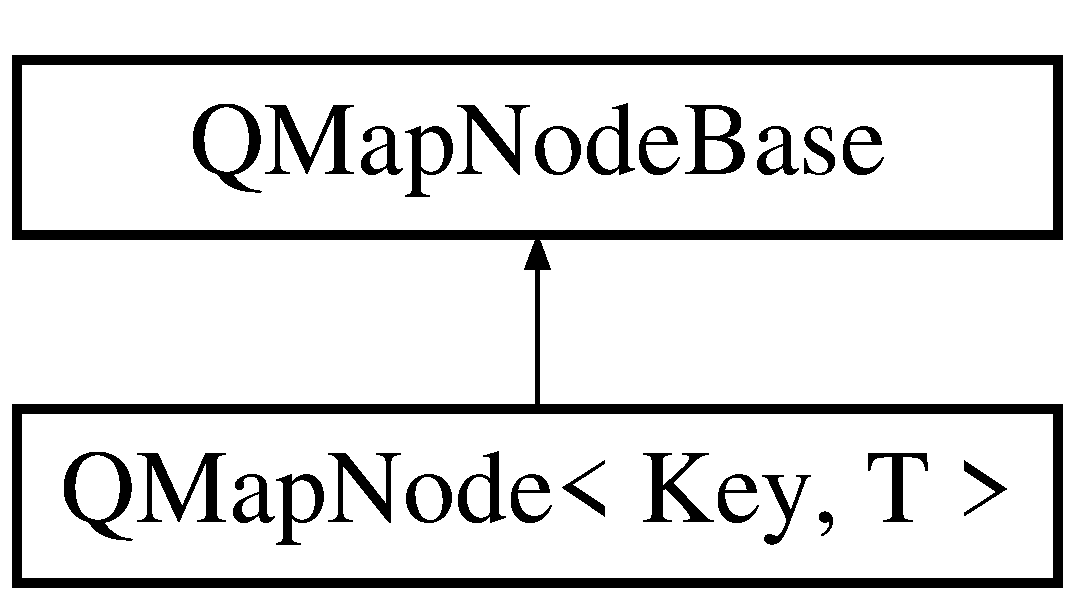
\includegraphics[height=2.000000cm]{struct_q_map_node_base}
\end{center}
\end{figure}
\subsection*{Public Types}
\begin{DoxyCompactItemize}
\item 
enum \hyperlink{struct_q_map_node_base_a8d262e109c5db0292c19141d585c96a9}{Color} \{ \hyperlink{struct_q_map_node_base_a8d262e109c5db0292c19141d585c96a9a9bffc80754cb87fa880417571e785e1b}{Red} = 0, 
\hyperlink{struct_q_map_node_base_a8d262e109c5db0292c19141d585c96a9a4a3c720b5a1ffee5b349ac2da8c5a2e1}{Black} = 1
 \}
\item 
enum \{ \hyperlink{struct_q_map_node_base_a98cd178a8587938441e879d638d4576cac454825c84685bfcd5173ffa84b23eb1}{Mask} = 3
 \}
\end{DoxyCompactItemize}
\subsection*{Public Member Functions}
\begin{DoxyCompactItemize}
\item 
const \hyperlink{struct_q_map_node_base}{Q\+Map\+Node\+Base} $\ast$ \hyperlink{struct_q_map_node_base_a0d003f88dea1eeda422c13636e2b0ff3}{next\+Node} () const 
\item 
\hyperlink{struct_q_map_node_base}{Q\+Map\+Node\+Base} $\ast$ \hyperlink{struct_q_map_node_base_a17a54c9b7145eb57325572c7b46da3f7}{next\+Node} ()
\item 
const \hyperlink{struct_q_map_node_base}{Q\+Map\+Node\+Base} $\ast$ \hyperlink{struct_q_map_node_base_a2036d1497e841434aa2bec59fd354036}{previous\+Node} () const 
\item 
\hyperlink{struct_q_map_node_base}{Q\+Map\+Node\+Base} $\ast$ \hyperlink{struct_q_map_node_base_af195b636253052fdd9aa8136e1d00169}{previous\+Node} ()
\item 
\hyperlink{struct_q_map_node_base_a8d262e109c5db0292c19141d585c96a9}{Color} \hyperlink{struct_q_map_node_base_ab9fd1e541601e17776f0eb3631f4722b}{color} () const 
\item 
void \hyperlink{struct_q_map_node_base_afe2e35dbcd8325173886c887447e88fc}{set\+Color} (\hyperlink{struct_q_map_node_base_a8d262e109c5db0292c19141d585c96a9}{Color} c)
\item 
\hyperlink{struct_q_map_node_base}{Q\+Map\+Node\+Base} $\ast$ \hyperlink{struct_q_map_node_base_ac41f93c0fbcab11e562fc760d78ec485}{parent} () const 
\item 
void \hyperlink{struct_q_map_node_base_a7846f9d0541b7e18680baf16bed97d9c}{set\+Parent} (\hyperlink{struct_q_map_node_base}{Q\+Map\+Node\+Base} $\ast$pp)
\end{DoxyCompactItemize}
\subsection*{Public Attributes}
\begin{DoxyCompactItemize}
\item 
quintptr \hyperlink{struct_q_map_node_base_a41743f32441f17a64e8faaf7f42d0bfb}{p}
\item 
\hyperlink{struct_q_map_node_base}{Q\+Map\+Node\+Base} $\ast$ \hyperlink{struct_q_map_node_base_a5334085d1e9ededc044ea0b5551ed7fd}{left}
\item 
\hyperlink{struct_q_map_node_base}{Q\+Map\+Node\+Base} $\ast$ \hyperlink{struct_q_map_node_base_a8eae5d979c668347872c31b956626a68}{right}
\end{DoxyCompactItemize}


\subsection{Detailed Description}


Definition at line 79 of file qmap.\+h.



\subsection{Member Enumeration Documentation}
\subsubsection[{\texorpdfstring{anonymous enum}{anonymous enum}}]{\setlength{\rightskip}{0pt plus 5cm}anonymous enum}\hypertarget{struct_q_map_node_base_a98cd178a8587938441e879d638d4576c}{}\label{struct_q_map_node_base_a98cd178a8587938441e879d638d4576c}
\begin{Desc}
\item[Enumerator]\par
\begin{description}
\index{Mask@{Mask}!Q\+Map\+Node\+Base@{Q\+Map\+Node\+Base}}\index{Q\+Map\+Node\+Base@{Q\+Map\+Node\+Base}!Mask@{Mask}}\item[{\em 
Mask\hypertarget{struct_q_map_node_base_a98cd178a8587938441e879d638d4576cac454825c84685bfcd5173ffa84b23eb1}{}\label{struct_q_map_node_base_a98cd178a8587938441e879d638d4576cac454825c84685bfcd5173ffa84b23eb1}
}]\end{description}
\end{Desc}


Definition at line 86 of file qmap.\+h.

\index{Q\+Map\+Node\+Base@{Q\+Map\+Node\+Base}!Color@{Color}}
\index{Color@{Color}!Q\+Map\+Node\+Base@{Q\+Map\+Node\+Base}}
\subsubsection[{\texorpdfstring{Color}{Color}}]{\setlength{\rightskip}{0pt plus 5cm}enum {\bf Q\+Map\+Node\+Base\+::\+Color}}\hypertarget{struct_q_map_node_base_a8d262e109c5db0292c19141d585c96a9}{}\label{struct_q_map_node_base_a8d262e109c5db0292c19141d585c96a9}
\begin{Desc}
\item[Enumerator]\par
\begin{description}
\index{Red@{Red}!Q\+Map\+Node\+Base@{Q\+Map\+Node\+Base}}\index{Q\+Map\+Node\+Base@{Q\+Map\+Node\+Base}!Red@{Red}}\item[{\em 
Red\hypertarget{struct_q_map_node_base_a8d262e109c5db0292c19141d585c96a9a9bffc80754cb87fa880417571e785e1b}{}\label{struct_q_map_node_base_a8d262e109c5db0292c19141d585c96a9a9bffc80754cb87fa880417571e785e1b}
}]\index{Black@{Black}!Q\+Map\+Node\+Base@{Q\+Map\+Node\+Base}}\index{Q\+Map\+Node\+Base@{Q\+Map\+Node\+Base}!Black@{Black}}\item[{\em 
Black\hypertarget{struct_q_map_node_base_a8d262e109c5db0292c19141d585c96a9a4a3c720b5a1ffee5b349ac2da8c5a2e1}{}\label{struct_q_map_node_base_a8d262e109c5db0292c19141d585c96a9a4a3c720b5a1ffee5b349ac2da8c5a2e1}
}]\end{description}
\end{Desc}


Definition at line 85 of file qmap.\+h.



\subsection{Member Function Documentation}
\index{Q\+Map\+Node\+Base@{Q\+Map\+Node\+Base}!color@{color}}
\index{color@{color}!Q\+Map\+Node\+Base@{Q\+Map\+Node\+Base}}
\subsubsection[{\texorpdfstring{color() const }{color() const }}]{\setlength{\rightskip}{0pt plus 5cm}{\bf Color} Q\+Map\+Node\+Base\+::color (
\begin{DoxyParamCaption}
{}
\end{DoxyParamCaption}
) const\hspace{0.3cm}{\ttfamily [inline]}}\hypertarget{struct_q_map_node_base_ab9fd1e541601e17776f0eb3631f4722b}{}\label{struct_q_map_node_base_ab9fd1e541601e17776f0eb3631f4722b}


Definition at line 93 of file qmap.\+h.

\index{Q\+Map\+Node\+Base@{Q\+Map\+Node\+Base}!next\+Node@{next\+Node}}
\index{next\+Node@{next\+Node}!Q\+Map\+Node\+Base@{Q\+Map\+Node\+Base}}
\subsubsection[{\texorpdfstring{next\+Node() const }{nextNode() const }}]{\setlength{\rightskip}{0pt plus 5cm}const {\bf Q\+Map\+Node\+Base} $\ast$ Q\+Map\+Node\+Base\+::next\+Node (
\begin{DoxyParamCaption}
{}
\end{DoxyParamCaption}
) const}\hypertarget{struct_q_map_node_base_a0d003f88dea1eeda422c13636e2b0ff3}{}\label{struct_q_map_node_base_a0d003f88dea1eeda422c13636e2b0ff3}


Definition at line 47 of file qmap.\+cpp.

\index{Q\+Map\+Node\+Base@{Q\+Map\+Node\+Base}!next\+Node@{next\+Node}}
\index{next\+Node@{next\+Node}!Q\+Map\+Node\+Base@{Q\+Map\+Node\+Base}}
\subsubsection[{\texorpdfstring{next\+Node()}{nextNode()}}]{\setlength{\rightskip}{0pt plus 5cm}{\bf Q\+Map\+Node\+Base}$\ast$ Q\+Map\+Node\+Base\+::next\+Node (
\begin{DoxyParamCaption}
{}
\end{DoxyParamCaption}
)\hspace{0.3cm}{\ttfamily [inline]}}\hypertarget{struct_q_map_node_base_a17a54c9b7145eb57325572c7b46da3f7}{}\label{struct_q_map_node_base_a17a54c9b7145eb57325572c7b46da3f7}


Definition at line 89 of file qmap.\+h.

\index{Q\+Map\+Node\+Base@{Q\+Map\+Node\+Base}!parent@{parent}}
\index{parent@{parent}!Q\+Map\+Node\+Base@{Q\+Map\+Node\+Base}}
\subsubsection[{\texorpdfstring{parent() const }{parent() const }}]{\setlength{\rightskip}{0pt plus 5cm}{\bf Q\+Map\+Node\+Base}$\ast$ Q\+Map\+Node\+Base\+::parent (
\begin{DoxyParamCaption}
{}
\end{DoxyParamCaption}
) const\hspace{0.3cm}{\ttfamily [inline]}}\hypertarget{struct_q_map_node_base_ac41f93c0fbcab11e562fc760d78ec485}{}\label{struct_q_map_node_base_ac41f93c0fbcab11e562fc760d78ec485}


Definition at line 95 of file qmap.\+h.

\index{Q\+Map\+Node\+Base@{Q\+Map\+Node\+Base}!previous\+Node@{previous\+Node}}
\index{previous\+Node@{previous\+Node}!Q\+Map\+Node\+Base@{Q\+Map\+Node\+Base}}
\subsubsection[{\texorpdfstring{previous\+Node() const }{previousNode() const }}]{\setlength{\rightskip}{0pt plus 5cm}const {\bf Q\+Map\+Node\+Base} $\ast$ Q\+Map\+Node\+Base\+::previous\+Node (
\begin{DoxyParamCaption}
{}
\end{DoxyParamCaption}
) const}\hypertarget{struct_q_map_node_base_a2036d1497e841434aa2bec59fd354036}{}\label{struct_q_map_node_base_a2036d1497e841434aa2bec59fd354036}


Definition at line 65 of file qmap.\+cpp.

\index{Q\+Map\+Node\+Base@{Q\+Map\+Node\+Base}!previous\+Node@{previous\+Node}}
\index{previous\+Node@{previous\+Node}!Q\+Map\+Node\+Base@{Q\+Map\+Node\+Base}}
\subsubsection[{\texorpdfstring{previous\+Node()}{previousNode()}}]{\setlength{\rightskip}{0pt plus 5cm}{\bf Q\+Map\+Node\+Base}$\ast$ Q\+Map\+Node\+Base\+::previous\+Node (
\begin{DoxyParamCaption}
{}
\end{DoxyParamCaption}
)\hspace{0.3cm}{\ttfamily [inline]}}\hypertarget{struct_q_map_node_base_af195b636253052fdd9aa8136e1d00169}{}\label{struct_q_map_node_base_af195b636253052fdd9aa8136e1d00169}


Definition at line 91 of file qmap.\+h.

\index{Q\+Map\+Node\+Base@{Q\+Map\+Node\+Base}!set\+Color@{set\+Color}}
\index{set\+Color@{set\+Color}!Q\+Map\+Node\+Base@{Q\+Map\+Node\+Base}}
\subsubsection[{\texorpdfstring{set\+Color(\+Color c)}{setColor(Color c)}}]{\setlength{\rightskip}{0pt plus 5cm}void Q\+Map\+Node\+Base\+::set\+Color (
\begin{DoxyParamCaption}
\item[{{\bf Color}}]{c}
\end{DoxyParamCaption}
)\hspace{0.3cm}{\ttfamily [inline]}}\hypertarget{struct_q_map_node_base_afe2e35dbcd8325173886c887447e88fc}{}\label{struct_q_map_node_base_afe2e35dbcd8325173886c887447e88fc}


Definition at line 94 of file qmap.\+h.

\index{Q\+Map\+Node\+Base@{Q\+Map\+Node\+Base}!set\+Parent@{set\+Parent}}
\index{set\+Parent@{set\+Parent}!Q\+Map\+Node\+Base@{Q\+Map\+Node\+Base}}
\subsubsection[{\texorpdfstring{set\+Parent(\+Q\+Map\+Node\+Base $\ast$pp)}{setParent(QMapNodeBase *pp)}}]{\setlength{\rightskip}{0pt plus 5cm}void Q\+Map\+Node\+Base\+::set\+Parent (
\begin{DoxyParamCaption}
\item[{{\bf Q\+Map\+Node\+Base} $\ast$}]{pp}
\end{DoxyParamCaption}
)\hspace{0.3cm}{\ttfamily [inline]}}\hypertarget{struct_q_map_node_base_a7846f9d0541b7e18680baf16bed97d9c}{}\label{struct_q_map_node_base_a7846f9d0541b7e18680baf16bed97d9c}


Definition at line 96 of file qmap.\+h.



\subsection{Member Data Documentation}
\index{Q\+Map\+Node\+Base@{Q\+Map\+Node\+Base}!left@{left}}
\index{left@{left}!Q\+Map\+Node\+Base@{Q\+Map\+Node\+Base}}
\subsubsection[{\texorpdfstring{left}{left}}]{\setlength{\rightskip}{0pt plus 5cm}{\bf Q\+Map\+Node\+Base}$\ast$ Q\+Map\+Node\+Base\+::left}\hypertarget{struct_q_map_node_base_a5334085d1e9ededc044ea0b5551ed7fd}{}\label{struct_q_map_node_base_a5334085d1e9ededc044ea0b5551ed7fd}


Definition at line 82 of file qmap.\+h.

\index{Q\+Map\+Node\+Base@{Q\+Map\+Node\+Base}!p@{p}}
\index{p@{p}!Q\+Map\+Node\+Base@{Q\+Map\+Node\+Base}}
\subsubsection[{\texorpdfstring{p}{p}}]{\setlength{\rightskip}{0pt plus 5cm}quintptr Q\+Map\+Node\+Base\+::p}\hypertarget{struct_q_map_node_base_a41743f32441f17a64e8faaf7f42d0bfb}{}\label{struct_q_map_node_base_a41743f32441f17a64e8faaf7f42d0bfb}


Definition at line 81 of file qmap.\+h.

\index{Q\+Map\+Node\+Base@{Q\+Map\+Node\+Base}!right@{right}}
\index{right@{right}!Q\+Map\+Node\+Base@{Q\+Map\+Node\+Base}}
\subsubsection[{\texorpdfstring{right}{right}}]{\setlength{\rightskip}{0pt plus 5cm}{\bf Q\+Map\+Node\+Base}$\ast$ Q\+Map\+Node\+Base\+::right}\hypertarget{struct_q_map_node_base_a8eae5d979c668347872c31b956626a68}{}\label{struct_q_map_node_base_a8eae5d979c668347872c31b956626a68}


Definition at line 83 of file qmap.\+h.



The documentation for this struct was generated from the following files\+:\begin{DoxyCompactItemize}
\item 
docs/extra-\/files/\hyperlink{qmap_8h}{qmap.\+h}\item 
docs/extra-\/files/\hyperlink{qmap_8cpp}{qmap.\+cpp}\end{DoxyCompactItemize}

\hypertarget{class_q_multi_map}{}\section{Q\+Multi\+Map$<$ Key, T $>$ Class Template Reference}
\label{class_q_multi_map}\index{Q\+Multi\+Map$<$ Key, T $>$@{Q\+Multi\+Map$<$ Key, T $>$}}


The \hyperlink{class_q_multi_map}{Q\+Multi\+Map} class is a convenience \hyperlink{class_q_map}{Q\+Map} subclass that provides multi-\/valued maps.  




{\ttfamily \#include $<$qmap.\+h$>$}

Inheritance diagram for Q\+Multi\+Map$<$ Key, T $>$\+:\begin{figure}[H]
\begin{center}
\leavevmode
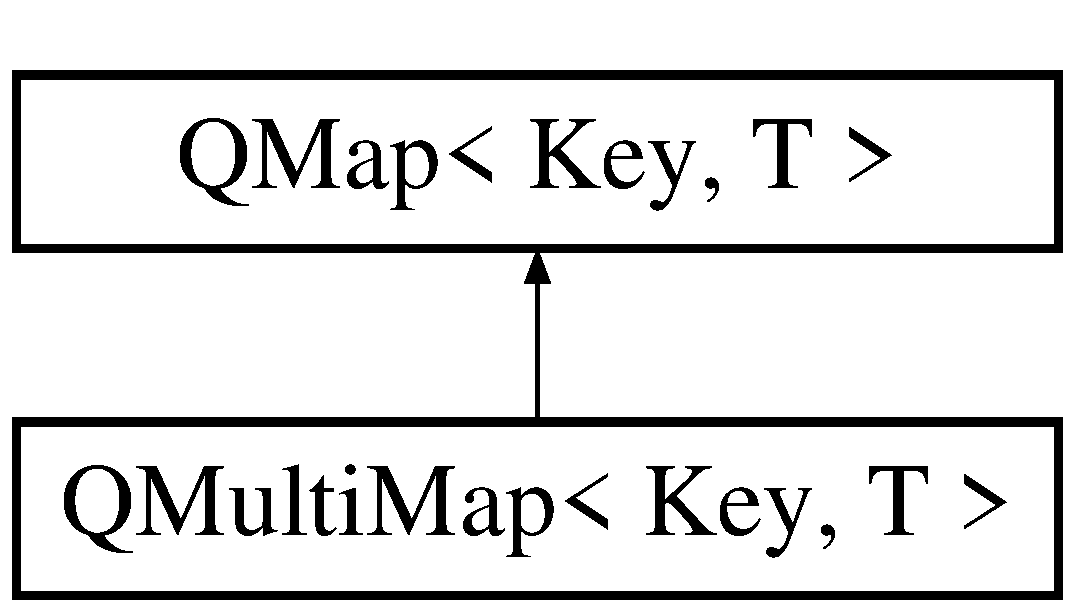
\includegraphics[height=2.000000cm]{class_q_multi_map}
\end{center}
\end{figure}
\subsection*{Public Member Functions}
\begin{DoxyCompactItemize}
\item 
\hyperlink{class_q_multi_map_aeb16603087ff81f07f9438de93528b66}{Q\+Multi\+Map} ()
\item 
\hyperlink{class_q_multi_map_a2e2af5d76f189e2bcbfe5c67b02df5e7}{Q\+Multi\+Map} (const \hyperlink{class_q_map}{Q\+Map}$<$ Key, T $>$ \&other)
\item 
void \hyperlink{class_q_multi_map_a1caa02d81e4487d753ec7cf63c509523}{swap} (\hyperlink{class_q_multi_map}{Q\+Multi\+Map}$<$ Key, T $>$ \&other)
\item 
\hyperlink{class_q_map}{Q\+Map}$<$ Key, T $>$\+::\hyperlink{class_q_map_1_1iterator}{iterator} \hyperlink{class_q_multi_map_a71c0ddeadd47b9410ef2d64c9fa24d72}{replace} (const Key \&\hyperlink{class_q_map_a7ad0c404885c5287fe593849e4bc80d6}{key}, const T \&\hyperlink{class_q_map_ab9c04f61f4abd94439d4431118a238e5}{value})
\item 
\hyperlink{class_q_map}{Q\+Map}$<$ Key, T $>$\+::\hyperlink{class_q_map_1_1iterator}{iterator} \hyperlink{class_q_multi_map_ae067c2f922dd6e13001d93ace23a964a}{insert} (const Key \&\hyperlink{class_q_map_a7ad0c404885c5287fe593849e4bc80d6}{key}, const T \&\hyperlink{class_q_map_ab9c04f61f4abd94439d4431118a238e5}{value})
\item 
\hyperlink{class_q_map}{Q\+Map}$<$ Key, T $>$\+::\hyperlink{class_q_map_1_1iterator}{iterator} \hyperlink{class_q_multi_map_a471e6ea8e6b77ab1a3fbcfd64c53bcf0}{insert} (typename \hyperlink{class_q_map}{Q\+Map}$<$ Key, T $>$\+::\hyperlink{class_q_map_1_1const__iterator}{const\+\_\+iterator} pos, const Key \&\hyperlink{class_q_map_a7ad0c404885c5287fe593849e4bc80d6}{key}, const T \&\hyperlink{class_q_map_ab9c04f61f4abd94439d4431118a238e5}{value})
\item 
\hyperlink{class_q_multi_map}{Q\+Multi\+Map} \& \hyperlink{class_q_multi_map_aa9c75ef8f14c919a318b494b54422958}{operator+=} (const \hyperlink{class_q_multi_map}{Q\+Multi\+Map} \&other)
\item 
\hyperlink{class_q_multi_map}{Q\+Multi\+Map} \hyperlink{class_q_multi_map_aef448db293ef347dca82cc017c559888}{operator+} (const \hyperlink{class_q_multi_map}{Q\+Multi\+Map} \&other) const 
\item 
bool \hyperlink{class_q_multi_map_ab240b90606e155eef7c80c2ea9cabe74}{contains} (const Key \&\hyperlink{class_q_map_a7ad0c404885c5287fe593849e4bc80d6}{key}, const T \&\hyperlink{class_q_map_ab9c04f61f4abd94439d4431118a238e5}{value}) const 
\item 
int \hyperlink{class_q_multi_map_a324e0c0f288ed749033c9df20efd88fa}{remove} (const Key \&\hyperlink{class_q_map_a7ad0c404885c5287fe593849e4bc80d6}{key}, const T \&\hyperlink{class_q_map_ab9c04f61f4abd94439d4431118a238e5}{value})
\item 
int \hyperlink{class_q_multi_map_abb89579656320a453ea7c80b2702d8c5}{count} (const Key \&\hyperlink{class_q_map_a7ad0c404885c5287fe593849e4bc80d6}{key}, const T \&\hyperlink{class_q_map_ab9c04f61f4abd94439d4431118a238e5}{value}) const 
\item 
\hyperlink{class_q_map}{Q\+Map}$<$ Key, T $>$\+::\hyperlink{class_q_map_1_1iterator}{iterator} \hyperlink{class_q_multi_map_ade33defb37a1abf5f4fff2686159afd4}{find} (const Key \&\hyperlink{class_q_map_a7ad0c404885c5287fe593849e4bc80d6}{key}, const T \&\hyperlink{class_q_map_ab9c04f61f4abd94439d4431118a238e5}{value})
\item 
\hyperlink{class_q_map}{Q\+Map}$<$ Key, T $>$\+::\hyperlink{class_q_map_1_1const__iterator}{const\+\_\+iterator} \hyperlink{class_q_multi_map_a84abf87a0d54493e9ecaa0e7fa4d5c62}{find} (const Key \&\hyperlink{class_q_map_a7ad0c404885c5287fe593849e4bc80d6}{key}, const T \&\hyperlink{class_q_map_ab9c04f61f4abd94439d4431118a238e5}{value}) const 
\item 
\hyperlink{class_q_map}{Q\+Map}$<$ Key, T $>$\+::\hyperlink{class_q_map_1_1const__iterator}{const\+\_\+iterator} \hyperlink{class_q_multi_map_ab0c0991e1c637c400b0d874f4a05b5ef}{const\+Find} (const Key \&\hyperlink{class_q_map_a7ad0c404885c5287fe593849e4bc80d6}{key}, const T \&\hyperlink{class_q_map_ab9c04f61f4abd94439d4431118a238e5}{value}) const 
\end{DoxyCompactItemize}
\subsection*{Additional Inherited Members}


\subsection{Detailed Description}
\subsubsection*{template$<$class Key, class T$>$\\*
class Q\+Multi\+Map$<$ Key, T $>$}

The \hyperlink{class_q_multi_map}{Q\+Multi\+Map} class is a convenience \hyperlink{class_q_map}{Q\+Map} subclass that provides multi-\/valued maps. 

Qt\+Core

\hyperlink{class_q_multi_map}{Q\+Multi\+Map}$<$Key, T$>$ is one of Qt\textquotesingle{}s generic \{container classes\}. It inherits \hyperlink{class_q_map}{Q\+Map} and extends it with a few convenience functions that make it more suitable than \hyperlink{class_q_map}{Q\+Map} for storing multi-\/valued maps. A multi-\/valued map is a map that allows multiple values with the same key; \hyperlink{class_q_map}{Q\+Map} normally doesn\textquotesingle{}t allow that, unless you call \hyperlink{class_q_map_a075634da2cf912a20dd1c4a5835acfa3}{Q\+Map\+::insert\+Multi()}.

Because \hyperlink{class_q_multi_map}{Q\+Multi\+Map} inherits \hyperlink{class_q_map}{Q\+Map}, all of \hyperlink{class_q_map}{Q\+Map}\textquotesingle{}s functionality also applies to \hyperlink{class_q_multi_map}{Q\+Multi\+Map}. For example, you can use \hyperlink{class_q_map_a33cfb24195273a5e70dcc48644368a99}{is\+Empty()} to test whether the map is empty, and you can traverse a \hyperlink{class_q_multi_map}{Q\+Multi\+Map} using \hyperlink{class_q_map}{Q\+Map}\textquotesingle{}s iterator classes (for example, Q\+Map\+Iterator). But in addition, it provides an \hyperlink{class_q_multi_map_ae067c2f922dd6e13001d93ace23a964a}{insert()} function that corresponds to \hyperlink{class_q_map_a075634da2cf912a20dd1c4a5835acfa3}{Q\+Map\+::insert\+Multi()}, and a \hyperlink{class_q_multi_map_a71c0ddeadd47b9410ef2d64c9fa24d72}{replace()} function that corresponds to \hyperlink{class_q_map_a0cc56ab47ea14af1127ac7399814d289}{Q\+Map\+::insert()}. It also provides convenient \hyperlink{class_q_multi_map_aef448db293ef347dca82cc017c559888}{operator+()} and \hyperlink{class_q_multi_map_aa9c75ef8f14c919a318b494b54422958}{operator+=()}.

Example\+: 
\begin{DoxyCodeInclude}
\end{DoxyCodeInclude}
 Unlike \hyperlink{class_q_map}{Q\+Map}, \hyperlink{class_q_multi_map}{Q\+Multi\+Map} provides no operator\mbox{[}\mbox{]}. Use \hyperlink{class_q_map_ab9c04f61f4abd94439d4431118a238e5}{value()} or \hyperlink{class_q_multi_map_a71c0ddeadd47b9410ef2d64c9fa24d72}{replace()} if you want to access the most recently inserted item with a certain key.

If you want to retrieve all the values for a single key, you can use values(const Key \&key), which returns a Q\+List$<$\+T$>$\+:


\begin{DoxyCodeInclude}
\end{DoxyCodeInclude}
 The items that share the same key are available from most recently to least recently inserted.

If you prefer the S\+T\+L-\/style iterators, you can call \hyperlink{class_q_multi_map_ade33defb37a1abf5f4fff2686159afd4}{find()} to get the iterator for the first item with a key and iterate from there\+:


\begin{DoxyCodeInclude}
\end{DoxyCodeInclude}
 \hyperlink{class_q_multi_map}{Q\+Multi\+Map}\textquotesingle{}s key and value data types must be \{assignable data types\}. This covers most data types you are likely to encounter, but the compiler won\textquotesingle{}t let you, for example, store a Q\+Widget as a value; instead, store a Q\+Widget $\ast$. In addition, \hyperlink{class_q_multi_map}{Q\+Multi\+Map}\textquotesingle{}s key type must provide operator$<$(). See the \hyperlink{class_q_map}{Q\+Map} documentation for details.

\begin{DoxySeeAlso}{See also}
\hyperlink{class_q_map}{Q\+Map}, Q\+Map\+Iterator, Q\+Mutable\+Map\+Iterator, Q\+Multi\+Hash 
\end{DoxySeeAlso}


Definition at line 1134 of file qmap.\+h.



\subsection{Constructor \& Destructor Documentation}
\index{Q\+Multi\+Map@{Q\+Multi\+Map}!Q\+Multi\+Map@{Q\+Multi\+Map}}
\index{Q\+Multi\+Map@{Q\+Multi\+Map}!Q\+Multi\+Map@{Q\+Multi\+Map}}
\subsubsection[{\texorpdfstring{Q\+Multi\+Map()}{QMultiMap()}}]{\setlength{\rightskip}{0pt plus 5cm}template$<$class Key, class T$>$ {\bf Q\+Multi\+Map}$<$ Key, T $>$\+::{\bf Q\+Multi\+Map} (
\begin{DoxyParamCaption}
{}
\end{DoxyParamCaption}
)\hspace{0.3cm}{\ttfamily [inline]}}\hypertarget{class_q_multi_map_aeb16603087ff81f07f9438de93528b66}{}\label{class_q_multi_map_aeb16603087ff81f07f9438de93528b66}
Constructs an empty map. 

Definition at line 1137 of file qmap.\+h.

\index{Q\+Multi\+Map@{Q\+Multi\+Map}!Q\+Multi\+Map@{Q\+Multi\+Map}}
\index{Q\+Multi\+Map@{Q\+Multi\+Map}!Q\+Multi\+Map@{Q\+Multi\+Map}}
\subsubsection[{\texorpdfstring{Q\+Multi\+Map(const Q\+Map$<$ Key, T $>$ \&other)}{QMultiMap(const QMap< Key, T > &other)}}]{\setlength{\rightskip}{0pt plus 5cm}template$<$class Key, class T$>$ {\bf Q\+Multi\+Map}$<$ Key, T $>$\+::{\bf Q\+Multi\+Map} (
\begin{DoxyParamCaption}
\item[{const {\bf Q\+Map}$<$ Key, T $>$ \&}]{other}
\end{DoxyParamCaption}
)\hspace{0.3cm}{\ttfamily [inline]}}\hypertarget{class_q_multi_map_a2e2af5d76f189e2bcbfe5c67b02df5e7}{}\label{class_q_multi_map_a2e2af5d76f189e2bcbfe5c67b02df5e7}
Constructs a copy of {\itshape other} (which can be a \hyperlink{class_q_map}{Q\+Map} or a \hyperlink{class_q_multi_map}{Q\+Multi\+Map}).

\begin{DoxySeeAlso}{See also}
\hyperlink{class_q_map_ad04759cfb5b1ed0f3d35a2a16f45ae54}{operator=()} 
\end{DoxySeeAlso}


Definition at line 1145 of file qmap.\+h.



\subsection{Member Function Documentation}
\index{Q\+Multi\+Map@{Q\+Multi\+Map}!const\+Find@{const\+Find}}
\index{const\+Find@{const\+Find}!Q\+Multi\+Map@{Q\+Multi\+Map}}
\subsubsection[{\texorpdfstring{const\+Find(const Key \&key, const T \&value) const }{constFind(const Key &key, const T &value) const }}]{\setlength{\rightskip}{0pt plus 5cm}template$<$class Key, class T$>$ typename {\bf Q\+Map}$<$ Key, T $>$\+::{\bf const\+\_\+iterator} {\bf Q\+Multi\+Map}$<$ Key, T $>$\+::const\+Find (
\begin{DoxyParamCaption}
\item[{const Key \&}]{key, }
\item[{const T \&}]{value}
\end{DoxyParamCaption}
) const\hspace{0.3cm}{\ttfamily [inline]}}\hypertarget{class_q_multi_map_ab0c0991e1c637c400b0d874f4a05b5ef}{}\label{class_q_multi_map_ab0c0991e1c637c400b0d874f4a05b5ef}
\begin{DoxySince}{Since}
4.\+3
\end{DoxySince}
Returns an iterator pointing to the item with key {\itshape key} and the value {\itshape value} in the map.

If the map contains no such item, the function returns \hyperlink{class_q_map_a6307f2d58e928bb15019024150f0afcb}{const\+End()}.

\begin{DoxySeeAlso}{See also}
\hyperlink{class_q_map_a4777a4aa1616ea8443c8b66bce74602f}{Q\+Map\+::const\+Find()} 
\end{DoxySeeAlso}


Definition at line 1192 of file qmap.\+h.

\index{Q\+Multi\+Map@{Q\+Multi\+Map}!contains@{contains}}
\index{contains@{contains}!Q\+Multi\+Map@{Q\+Multi\+Map}}
\subsubsection[{\texorpdfstring{contains(const Key \&key, const T \&value) const }{contains(const Key &key, const T &value) const }}]{\setlength{\rightskip}{0pt plus 5cm}template$<$class Key , class T $>$ Q\+\_\+\+I\+N\+L\+I\+N\+E\+\_\+\+T\+E\+M\+P\+L\+A\+TE bool {\bf Q\+Multi\+Map}$<$ Key, T $>$\+::contains (
\begin{DoxyParamCaption}
\item[{const Key \&}]{key, }
\item[{const T \&}]{value}
\end{DoxyParamCaption}
) const}\hypertarget{class_q_multi_map_ab240b90606e155eef7c80c2ea9cabe74}{}\label{class_q_multi_map_ab240b90606e155eef7c80c2ea9cabe74}
\begin{DoxySince}{Since}
4.\+3
\end{DoxySince}
Returns {\ttfamily true} if the map contains an item with key {\itshape key} and value {\itshape value}; otherwise returns {\ttfamily false}.

\begin{DoxySeeAlso}{See also}
\hyperlink{class_q_map_ac92f0cafb70425a2d3d5171cf367dd11}{Q\+Map\+::contains()} 
\end{DoxySeeAlso}


Definition at line 1200 of file qmap.\+h.

\index{Q\+Multi\+Map@{Q\+Multi\+Map}!count@{count}}
\index{count@{count}!Q\+Multi\+Map@{Q\+Multi\+Map}}
\subsubsection[{\texorpdfstring{count(const Key \&key, const T \&value) const }{count(const Key &key, const T &value) const }}]{\setlength{\rightskip}{0pt plus 5cm}template$<$class Key , class T $>$ Q\+\_\+\+I\+N\+L\+I\+N\+E\+\_\+\+T\+E\+M\+P\+L\+A\+TE int {\bf Q\+Multi\+Map}$<$ Key, T $>$\+::count (
\begin{DoxyParamCaption}
\item[{const Key \&}]{key, }
\item[{const T \&}]{value}
\end{DoxyParamCaption}
) const}\hypertarget{class_q_multi_map_abb89579656320a453ea7c80b2702d8c5}{}\label{class_q_multi_map_abb89579656320a453ea7c80b2702d8c5}
\begin{DoxySince}{Since}
4.\+3
\end{DoxySince}
Returns the number of items with key {\itshape key} and value {\itshape value}.

\begin{DoxySeeAlso}{See also}
\hyperlink{class_q_map_a7576304b0025dbb0f127c655c05377ac}{Q\+Map\+::count()} 
\end{DoxySeeAlso}


Definition at line 1223 of file qmap.\+h.

\index{Q\+Multi\+Map@{Q\+Multi\+Map}!find@{find}}
\index{find@{find}!Q\+Multi\+Map@{Q\+Multi\+Map}}
\subsubsection[{\texorpdfstring{find(const Key \&key, const T \&value)}{find(const Key &key, const T &value)}}]{\setlength{\rightskip}{0pt plus 5cm}template$<$class Key, class T$>$ typename {\bf Q\+Map}$<$ Key, T $>$\+::{\bf iterator} {\bf Q\+Multi\+Map}$<$ Key, T $>$\+::find (
\begin{DoxyParamCaption}
\item[{const Key \&}]{key, }
\item[{const T \&}]{value}
\end{DoxyParamCaption}
)\hspace{0.3cm}{\ttfamily [inline]}}\hypertarget{class_q_multi_map_ade33defb37a1abf5f4fff2686159afd4}{}\label{class_q_multi_map_ade33defb37a1abf5f4fff2686159afd4}
\begin{DoxySince}{Since}
4.\+3
\end{DoxySince}
Returns an iterator pointing to the item with key {\itshape key} and value {\itshape value} in the map.

If the map contains no such item, the function returns \hyperlink{class_q_map_a2935881385191efbb074e96cf8d3c9b6}{end()}.

If the map contains multiple items with key {\itshape key}, this function returns an iterator that points to the most recently inserted value.

\begin{DoxySeeAlso}{See also}
\hyperlink{class_q_map_a8cf44b635018eb178cc724ed20379d85}{Q\+Map\+::find()} 
\end{DoxySeeAlso}


Definition at line 1172 of file qmap.\+h.

\index{Q\+Multi\+Map@{Q\+Multi\+Map}!find@{find}}
\index{find@{find}!Q\+Multi\+Map@{Q\+Multi\+Map}}
\subsubsection[{\texorpdfstring{find(const Key \&key, const T \&value) const }{find(const Key &key, const T &value) const }}]{\setlength{\rightskip}{0pt plus 5cm}template$<$class Key, class T$>$ typename {\bf Q\+Map}$<$ Key, T $>$\+::{\bf const\+\_\+iterator} {\bf Q\+Multi\+Map}$<$ Key, T $>$\+::find (
\begin{DoxyParamCaption}
\item[{const Key \&}]{key, }
\item[{const T \&}]{value}
\end{DoxyParamCaption}
) const\hspace{0.3cm}{\ttfamily [inline]}}\hypertarget{class_q_multi_map_a84abf87a0d54493e9ecaa0e7fa4d5c62}{}\label{class_q_multi_map_a84abf87a0d54493e9ecaa0e7fa4d5c62}
\begin{DoxySince}{Since}
4.\+3 This is an overloaded member function, provided for convenience. It differs from the above function only in what argument(s) it accepts.
\end{DoxySince}
Returns a const iterator pointing to the item with the given {\itshape key} and {\itshape value} in the map.

If the map contains no such item, the function returns \hyperlink{class_q_map_a2935881385191efbb074e96cf8d3c9b6}{end()}.

If the map contains multiple items with the specified {\itshape key}, this function returns a const iterator that points to the most recently inserted value.

\begin{DoxySeeAlso}{See also}
\hyperlink{class_q_map_a8cf44b635018eb178cc724ed20379d85}{Q\+Map\+::find()} 
\end{DoxySeeAlso}


Definition at line 1182 of file qmap.\+h.

\index{Q\+Multi\+Map@{Q\+Multi\+Map}!insert@{insert}}
\index{insert@{insert}!Q\+Multi\+Map@{Q\+Multi\+Map}}
\subsubsection[{\texorpdfstring{insert(const Key \&key, const T \&value)}{insert(const Key &key, const T &value)}}]{\setlength{\rightskip}{0pt plus 5cm}template$<$class Key, class T$>$ {\bf Q\+Multi\+Map\+::iterator} {\bf Q\+Multi\+Map}$<$ Key, T $>$\+::insert (
\begin{DoxyParamCaption}
\item[{const Key \&}]{key, }
\item[{const T \&}]{value}
\end{DoxyParamCaption}
)\hspace{0.3cm}{\ttfamily [inline]}}\hypertarget{class_q_multi_map_ae067c2f922dd6e13001d93ace23a964a}{}\label{class_q_multi_map_ae067c2f922dd6e13001d93ace23a964a}
Inserts a new item with the key {\itshape key} and a value of {\itshape value}.

If there is already an item with the same key in the map, this function will simply create a new one. (This behavior is different from \hyperlink{class_q_multi_map_a71c0ddeadd47b9410ef2d64c9fa24d72}{replace()}, which overwrites the value of an existing item.)

\begin{DoxySeeAlso}{See also}
\hyperlink{class_q_multi_map_a71c0ddeadd47b9410ef2d64c9fa24d72}{replace()} 
\end{DoxySeeAlso}


Definition at line 1150 of file qmap.\+h.

\index{Q\+Multi\+Map@{Q\+Multi\+Map}!insert@{insert}}
\index{insert@{insert}!Q\+Multi\+Map@{Q\+Multi\+Map}}
\subsubsection[{\texorpdfstring{insert(typename Q\+Map$<$ Key, T $>$\+::const\+\_\+iterator pos, const Key \&key, const T \&value)}{insert(typename QMap< Key, T >::const_iterator pos, const Key &key, const T &value)}}]{\setlength{\rightskip}{0pt plus 5cm}template$<$class Key, class T$>$ {\bf Q\+Multi\+Map\+::iterator} {\bf Q\+Multi\+Map}$<$ Key, T $>$\+::insert (
\begin{DoxyParamCaption}
\item[{typename {\bf Q\+Map}$<$ Key, T $>$\+::{\bf const\+\_\+iterator}}]{pos, }
\item[{const Key \&}]{key, }
\item[{const T \&}]{value}
\end{DoxyParamCaption}
)\hspace{0.3cm}{\ttfamily [inline]}}\hypertarget{class_q_multi_map_a471e6ea8e6b77ab1a3fbcfd64c53bcf0}{}\label{class_q_multi_map_a471e6ea8e6b77ab1a3fbcfd64c53bcf0}
\begin{DoxySince}{Since}
5.\+1 Inserts a new item with the key {\itshape key} and value {\itshape value} and with hint {\itshape pos} suggesting where to do the insert.
\end{DoxySince}
If \hyperlink{class_q_map_ab55b01ac2790d09ceff0b911474a8b43}{const\+Begin()} is used as hint it indicates that the {\itshape key} is less than any key in the map while \hyperlink{class_q_map_a6307f2d58e928bb15019024150f0afcb}{const\+End()} suggests that the {\itshape key} is larger than any key in the map. Otherwise the hint should meet the condition ({\itshape pos} -\/ 1).\hyperlink{class_q_map_a7ad0c404885c5287fe593849e4bc80d6}{key()} $<$ {\itshape key} $<$= pos.\+key(). If the hint {\itshape pos} is wrong it is ignored and a regular insert is done.

If there is already an item with the same key in the map, this function will simply create a new one.

{\bfseries \{Note\+:\}} Be careful with the hint. Providing an iterator from an older shared instance might crash but there is also a risk that it will silently corrupt both the map and the {\itshape pos} map. 

Definition at line 1152 of file qmap.\+h.

\index{Q\+Multi\+Map@{Q\+Multi\+Map}!operator+@{operator+}}
\index{operator+@{operator+}!Q\+Multi\+Map@{Q\+Multi\+Map}}
\subsubsection[{\texorpdfstring{operator+(const Q\+Multi\+Map \&other) const }{operator+(const QMultiMap &other) const }}]{\setlength{\rightskip}{0pt plus 5cm}template$<$class Key, class T$>$ {\bf Q\+Multi\+Map} {\bf Q\+Multi\+Map}$<$ Key, T $>$\+::operator+ (
\begin{DoxyParamCaption}
\item[{const {\bf Q\+Multi\+Map}$<$ Key, T $>$ \&}]{other}
\end{DoxyParamCaption}
) const\hspace{0.3cm}{\ttfamily [inline]}}\hypertarget{class_q_multi_map_aef448db293ef347dca82cc017c559888}{}\label{class_q_multi_map_aef448db293ef347dca82cc017c559888}
Returns a map that contains all the items in this map in addition to all the items in {\itshape other}. If a key is common to both maps, the resulting map will contain the key multiple times.

\begin{DoxySeeAlso}{See also}
\hyperlink{class_q_multi_map_aa9c75ef8f14c919a318b494b54422958}{operator+=()} 
\end{DoxySeeAlso}


Definition at line 1157 of file qmap.\+h.

\index{Q\+Multi\+Map@{Q\+Multi\+Map}!operator+=@{operator+=}}
\index{operator+=@{operator+=}!Q\+Multi\+Map@{Q\+Multi\+Map}}
\subsubsection[{\texorpdfstring{operator+=(const Q\+Multi\+Map \&other)}{operator+=(const QMultiMap &other)}}]{\setlength{\rightskip}{0pt plus 5cm}template$<$class Key, class T$>$ {\bf Q\+Multi\+Map} \& {\bf Q\+Multi\+Map}$<$ Key, T $>$\+::operator+= (
\begin{DoxyParamCaption}
\item[{const {\bf Q\+Multi\+Map}$<$ Key, T $>$ \&}]{other}
\end{DoxyParamCaption}
)\hspace{0.3cm}{\ttfamily [inline]}}\hypertarget{class_q_multi_map_aa9c75ef8f14c919a318b494b54422958}{}\label{class_q_multi_map_aa9c75ef8f14c919a318b494b54422958}
Inserts all the items in the {\itshape other} map into this map and returns a reference to this map.

\begin{DoxySeeAlso}{See also}
\hyperlink{class_q_multi_map_ae067c2f922dd6e13001d93ace23a964a}{insert()}, \hyperlink{class_q_multi_map_aef448db293ef347dca82cc017c559888}{operator+()} 
\end{DoxySeeAlso}


Definition at line 1155 of file qmap.\+h.

\index{Q\+Multi\+Map@{Q\+Multi\+Map}!remove@{remove}}
\index{remove@{remove}!Q\+Multi\+Map@{Q\+Multi\+Map}}
\subsubsection[{\texorpdfstring{remove(const Key \&key, const T \&value)}{remove(const Key &key, const T &value)}}]{\setlength{\rightskip}{0pt plus 5cm}template$<$class Key , class T $>$ Q\+\_\+\+I\+N\+L\+I\+N\+E\+\_\+\+T\+E\+M\+P\+L\+A\+TE int {\bf Q\+Multi\+Map}$<$ Key, T $>$\+::remove (
\begin{DoxyParamCaption}
\item[{const Key \&}]{key, }
\item[{const T \&}]{value}
\end{DoxyParamCaption}
)}\hypertarget{class_q_multi_map_a324e0c0f288ed749033c9df20efd88fa}{}\label{class_q_multi_map_a324e0c0f288ed749033c9df20efd88fa}
\begin{DoxySince}{Since}
4.\+3
\end{DoxySince}
Removes all the items that have the key {\itshape key} and the value {\itshape value} from the map. Returns the number of items removed.

\begin{DoxySeeAlso}{See also}
\hyperlink{class_q_map_af562610e90763fad449dfc130bd18fb8}{Q\+Map\+::remove()} 
\end{DoxySeeAlso}


Definition at line 1206 of file qmap.\+h.

\index{Q\+Multi\+Map@{Q\+Multi\+Map}!replace@{replace}}
\index{replace@{replace}!Q\+Multi\+Map@{Q\+Multi\+Map}}
\subsubsection[{\texorpdfstring{replace(const Key \&key, const T \&value)}{replace(const Key &key, const T &value)}}]{\setlength{\rightskip}{0pt plus 5cm}template$<$class Key, class T$>$ {\bf Q\+Multi\+Map\+::iterator} {\bf Q\+Multi\+Map}$<$ Key, T $>$\+::replace (
\begin{DoxyParamCaption}
\item[{const Key \&}]{key, }
\item[{const T \&}]{value}
\end{DoxyParamCaption}
)\hspace{0.3cm}{\ttfamily [inline]}}\hypertarget{class_q_multi_map_a71c0ddeadd47b9410ef2d64c9fa24d72}{}\label{class_q_multi_map_a71c0ddeadd47b9410ef2d64c9fa24d72}
Inserts a new item with the key {\itshape key} and a value of {\itshape value}.

If there is already an item with the key {\itshape key}, that item\textquotesingle{}s value is replaced with {\itshape value}.

If there are multiple items with the key {\itshape key}, the most recently inserted item\textquotesingle{}s value is replaced with {\itshape value}.

\begin{DoxySeeAlso}{See also}
\hyperlink{class_q_multi_map_ae067c2f922dd6e13001d93ace23a964a}{insert()} 
\end{DoxySeeAlso}


Definition at line 1148 of file qmap.\+h.

\index{Q\+Multi\+Map@{Q\+Multi\+Map}!swap@{swap}}
\index{swap@{swap}!Q\+Multi\+Map@{Q\+Multi\+Map}}
\subsubsection[{\texorpdfstring{swap(\+Q\+Multi\+Map$<$ Key, T $>$ \&other)}{swap(QMultiMap< Key, T > &other)}}]{\setlength{\rightskip}{0pt plus 5cm}template$<$class Key, class T$>$ void {\bf Q\+Multi\+Map}$<$ Key, T $>$\+::swap (
\begin{DoxyParamCaption}
\item[{{\bf Q\+Multi\+Map}$<$ Key, T $>$ \&}]{other}
\end{DoxyParamCaption}
)\hspace{0.3cm}{\ttfamily [inline]}}\hypertarget{class_q_multi_map_a1caa02d81e4487d753ec7cf63c509523}{}\label{class_q_multi_map_a1caa02d81e4487d753ec7cf63c509523}
\begin{DoxySince}{Since}
4.\+8
\end{DoxySince}
Swaps map {\itshape other} with this map. This operation is very fast and never fails. 

Definition at line 1146 of file qmap.\+h.



The documentation for this class was generated from the following files\+:\begin{DoxyCompactItemize}
\item 
docs/extra-\/files/\hyperlink{qmap_8h}{qmap.\+h}\item 
docs/extra-\/files/\hyperlink{qmap_8cpp}{qmap.\+cpp}\end{DoxyCompactItemize}

\hypertarget{class_q_set}{}\section{Q\+Set$<$ T $>$ Class Template Reference}
\label{class_q_set}\index{Q\+Set$<$ T $>$@{Q\+Set$<$ T $>$}}


{\ttfamily \#include $<$qlist.\+h$>$}



\subsection{Detailed Description}
\subsubsection*{template$<$typename T$>$\\*
class Q\+Set$<$ T $>$}



Definition at line 63 of file qlist.\+h.



The documentation for this class was generated from the following file\+:\begin{DoxyCompactItemize}
\item 
docs/extra-\/files/\hyperlink{qlist_8h}{qlist.\+h}\end{DoxyCompactItemize}

\hypertarget{class_q_stack}{}\section{Q\+Stack$<$ T $>$ Class Template Reference}
\label{class_q_stack}\index{Q\+Stack$<$ T $>$@{Q\+Stack$<$ T $>$}}


The \hyperlink{class_q_stack}{Q\+Stack} class is a template class that provides a stack.  




{\ttfamily \#include $<$qstack.\+h$>$}

Inheritance diagram for Q\+Stack$<$ T $>$\+:\begin{figure}[H]
\begin{center}
\leavevmode
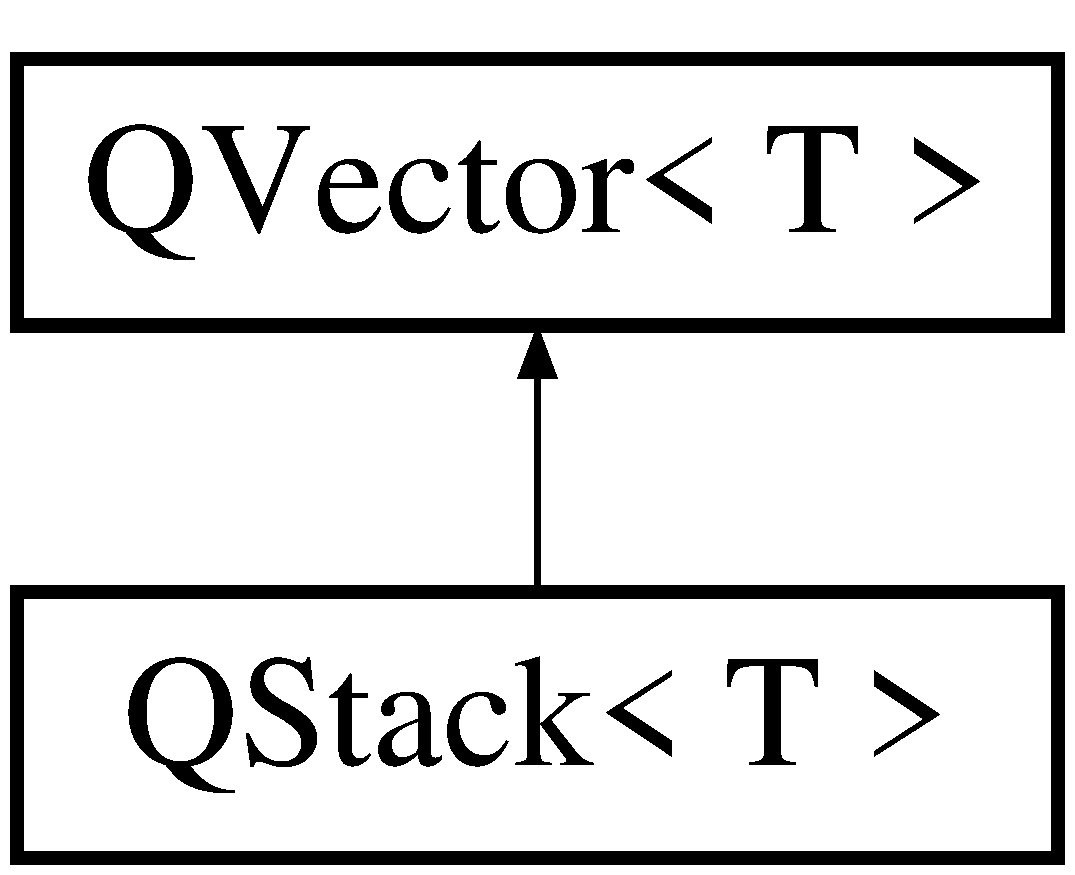
\includegraphics[height=2.000000cm]{class_q_stack}
\end{center}
\end{figure}
\subsection*{Public Member Functions}
\begin{DoxyCompactItemize}
\item 
\hyperlink{class_q_stack_ab42514d12612ebaf86f9db5068eaf390}{Q\+Stack} ()
\item 
\hyperlink{class_q_stack_ab0a0458193135b516c7a083ac8a3d4a2}{$\sim$\+Q\+Stack} ()
\item 
void \hyperlink{class_q_stack_afc2b34603e880f6ccf533835a407d601}{swap} (\hyperlink{class_q_stack}{Q\+Stack}$<$ T $>$ \&other)
\item 
void \hyperlink{class_q_stack_afe6cdb317571080fa991ba998db2801e}{push} (const T \&t)
\item 
T \hyperlink{class_q_stack_ad2944420ebf35829a8f7c54d75ea8a35}{pop} ()
\item 
T \& \hyperlink{class_q_stack_a3253bfc5509f9c4afffe60b10326961d}{top} ()
\item 
const T \& \hyperlink{class_q_stack_ad5942029d173afac32132085f7f140db}{top} () const 
\end{DoxyCompactItemize}
\subsection*{Additional Inherited Members}


\subsection{Detailed Description}
\subsubsection*{template$<$class T$>$\\*
class Q\+Stack$<$ T $>$}

The \hyperlink{class_q_stack}{Q\+Stack} class is a template class that provides a stack. 

Qt\+Core

\hyperlink{class_q_stack}{Q\+Stack}$<$T$>$ is one of Qt\textquotesingle{}s generic \{container classes\}. It implements a stack data structure for items of a same type.

A stack is a last in, first out (L\+I\+FO) structure. Items are added to the top of the stack using \hyperlink{class_q_stack_afe6cdb317571080fa991ba998db2801e}{push()} and retrieved from the top using \hyperlink{class_q_stack_ad2944420ebf35829a8f7c54d75ea8a35}{pop()}. The \hyperlink{class_q_stack_a3253bfc5509f9c4afffe60b10326961d}{top()} function provides access to the topmost item without removing it.

Example\+:


\begin{DoxyCodeInclude}
\end{DoxyCodeInclude}
 The example will output 3, 2, 1 in that order.

\hyperlink{class_q_stack}{Q\+Stack} inherits from \hyperlink{class_q_vector}{Q\+Vector}. All of \hyperlink{class_q_vector}{Q\+Vector}\textquotesingle{}s functionality also applies to \hyperlink{class_q_stack}{Q\+Stack}. For example, you can use \hyperlink{class_q_vector_a23ddd6fbfe38f8c34f69b5af89e97000}{is\+Empty()} to test whether the stack is empty, and you can traverse a \hyperlink{class_q_stack}{Q\+Stack} using \hyperlink{class_q_vector}{Q\+Vector}\textquotesingle{}s iterator classes (for example, Q\+Vector\+Iterator). But in addition, \hyperlink{class_q_stack}{Q\+Stack} provides three convenience functions that make it easy to implement L\+I\+FO semantics\+: \hyperlink{class_q_stack_afe6cdb317571080fa991ba998db2801e}{push()}, \hyperlink{class_q_stack_ad2944420ebf35829a8f7c54d75ea8a35}{pop()}, and \hyperlink{class_q_stack_a3253bfc5509f9c4afffe60b10326961d}{top()}.

\hyperlink{class_q_stack}{Q\+Stack}\textquotesingle{}s value type must be an \{assignable data type\}. This covers most data types that are commonly used, but the compiler won\textquotesingle{}t let you, for example, store a Q\+Widget as a value; instead, store a Q\+Widget $\ast$.

\begin{DoxySeeAlso}{See also}
\hyperlink{class_q_vector}{Q\+Vector}, Q\+Queue 
\end{DoxySeeAlso}


Definition at line 43 of file qstack.\+h.



\subsection{Constructor \& Destructor Documentation}
\index{Q\+Stack@{Q\+Stack}!Q\+Stack@{Q\+Stack}}
\index{Q\+Stack@{Q\+Stack}!Q\+Stack@{Q\+Stack}}
\subsubsection[{\texorpdfstring{Q\+Stack()}{QStack()}}]{\setlength{\rightskip}{0pt plus 5cm}template$<$class T$>$ {\bf Q\+Stack}$<$ T $>$\+::{\bf Q\+Stack} (
\begin{DoxyParamCaption}
{}
\end{DoxyParamCaption}
)\hspace{0.3cm}{\ttfamily [inline]}}\hypertarget{class_q_stack_ab42514d12612ebaf86f9db5068eaf390}{}\label{class_q_stack_ab42514d12612ebaf86f9db5068eaf390}
Constructs an empty stack. 

Definition at line 46 of file qstack.\+h.

\index{Q\+Stack@{Q\+Stack}!````~Q\+Stack@{$\sim$\+Q\+Stack}}
\index{````~Q\+Stack@{$\sim$\+Q\+Stack}!Q\+Stack@{Q\+Stack}}
\subsubsection[{\texorpdfstring{$\sim$\+Q\+Stack()}{~QStack()}}]{\setlength{\rightskip}{0pt plus 5cm}template$<$class T$>$ {\bf Q\+Stack}$<$ T $>$\+::$\sim${\bf Q\+Stack} (
\begin{DoxyParamCaption}
{}
\end{DoxyParamCaption}
)\hspace{0.3cm}{\ttfamily [inline]}}\hypertarget{class_q_stack_ab0a0458193135b516c7a083ac8a3d4a2}{}\label{class_q_stack_ab0a0458193135b516c7a083ac8a3d4a2}
Destroys the stack. References to the values in the stack, and all iterators over this stack, become invalid. 

Definition at line 47 of file qstack.\+h.



\subsection{Member Function Documentation}
\index{Q\+Stack@{Q\+Stack}!pop@{pop}}
\index{pop@{pop}!Q\+Stack@{Q\+Stack}}
\subsubsection[{\texorpdfstring{pop()}{pop()}}]{\setlength{\rightskip}{0pt plus 5cm}template$<$class T $>$ T {\bf Q\+Stack}$<$ T $>$\+::pop (
\begin{DoxyParamCaption}
{}
\end{DoxyParamCaption}
)\hspace{0.3cm}{\ttfamily [inline]}}\hypertarget{class_q_stack_ad2944420ebf35829a8f7c54d75ea8a35}{}\label{class_q_stack_ad2944420ebf35829a8f7c54d75ea8a35}
Removes the top item from the stack and returns it. This function assumes that the stack isn\textquotesingle{}t empty.

\begin{DoxySeeAlso}{See also}
\hyperlink{class_q_stack_a3253bfc5509f9c4afffe60b10326961d}{top()}, \hyperlink{class_q_stack_afe6cdb317571080fa991ba998db2801e}{push()}, \hyperlink{class_q_vector_a23ddd6fbfe38f8c34f69b5af89e97000}{is\+Empty()} 
\end{DoxySeeAlso}


Definition at line 56 of file qstack.\+h.

\index{Q\+Stack@{Q\+Stack}!push@{push}}
\index{push@{push}!Q\+Stack@{Q\+Stack}}
\subsubsection[{\texorpdfstring{push(const T \&t)}{push(const T &t)}}]{\setlength{\rightskip}{0pt plus 5cm}template$<$class T$>$ void {\bf Q\+Stack}$<$ T $>$\+::push (
\begin{DoxyParamCaption}
\item[{const T \&}]{t}
\end{DoxyParamCaption}
)\hspace{0.3cm}{\ttfamily [inline]}}\hypertarget{class_q_stack_afe6cdb317571080fa991ba998db2801e}{}\label{class_q_stack_afe6cdb317571080fa991ba998db2801e}
Adds element {\itshape t} to the top of the stack.

This is the same as \hyperlink{class_q_vector_ad3536b6c85748f8b0b376d5d9ba0e721}{Q\+Vector\+::append()}.

\begin{DoxySeeAlso}{See also}
\hyperlink{class_q_stack_ad2944420ebf35829a8f7c54d75ea8a35}{pop()}, \hyperlink{class_q_stack_a3253bfc5509f9c4afffe60b10326961d}{top()} 
\end{DoxySeeAlso}


Definition at line 49 of file qstack.\+h.

\index{Q\+Stack@{Q\+Stack}!swap@{swap}}
\index{swap@{swap}!Q\+Stack@{Q\+Stack}}
\subsubsection[{\texorpdfstring{swap(\+Q\+Stack$<$ T $>$ \&other)}{swap(QStack< T > &other)}}]{\setlength{\rightskip}{0pt plus 5cm}template$<$class T$>$ void {\bf Q\+Stack}$<$ T $>$\+::swap (
\begin{DoxyParamCaption}
\item[{{\bf Q\+Stack}$<$ T $>$ \&}]{other}
\end{DoxyParamCaption}
)\hspace{0.3cm}{\ttfamily [inline]}}\hypertarget{class_q_stack_afc2b34603e880f6ccf533835a407d601}{}\label{class_q_stack_afc2b34603e880f6ccf533835a407d601}
\begin{DoxySince}{Since}
4.\+8
\end{DoxySince}
Swaps stack {\itshape other} with this stack. This operation is very fast and never fails. 

Definition at line 48 of file qstack.\+h.

\index{Q\+Stack@{Q\+Stack}!top@{top}}
\index{top@{top}!Q\+Stack@{Q\+Stack}}
\subsubsection[{\texorpdfstring{top()}{top()}}]{\setlength{\rightskip}{0pt plus 5cm}template$<$class T $>$ T \& {\bf Q\+Stack}$<$ T $>$\+::top (
\begin{DoxyParamCaption}
{}
\end{DoxyParamCaption}
)\hspace{0.3cm}{\ttfamily [inline]}}\hypertarget{class_q_stack_a3253bfc5509f9c4afffe60b10326961d}{}\label{class_q_stack_a3253bfc5509f9c4afffe60b10326961d}
Returns a reference to the stack\textquotesingle{}s top item. This function assumes that the stack isn\textquotesingle{}t empty.

This is the same as \hyperlink{class_q_vector_a93f335707c6d1003dd2b594e4066ed0b}{Q\+Vector\+::last()}.

\begin{DoxySeeAlso}{See also}
\hyperlink{class_q_stack_ad2944420ebf35829a8f7c54d75ea8a35}{pop()}, \hyperlink{class_q_stack_afe6cdb317571080fa991ba998db2801e}{push()}, \hyperlink{class_q_vector_a23ddd6fbfe38f8c34f69b5af89e97000}{is\+Empty()} 
\end{DoxySeeAlso}


Definition at line 61 of file qstack.\+h.

\index{Q\+Stack@{Q\+Stack}!top@{top}}
\index{top@{top}!Q\+Stack@{Q\+Stack}}
\subsubsection[{\texorpdfstring{top() const }{top() const }}]{\setlength{\rightskip}{0pt plus 5cm}template$<$class T $>$ const T \& {\bf Q\+Stack}$<$ T $>$\+::top (
\begin{DoxyParamCaption}
{}
\end{DoxyParamCaption}
) const\hspace{0.3cm}{\ttfamily [inline]}}\hypertarget{class_q_stack_ad5942029d173afac32132085f7f140db}{}\label{class_q_stack_ad5942029d173afac32132085f7f140db}
This is an overloaded member function, provided for convenience. It differs from the above function only in what argument(s) it accepts.

\begin{DoxySeeAlso}{See also}
\hyperlink{class_q_stack_ad2944420ebf35829a8f7c54d75ea8a35}{pop()}, \hyperlink{class_q_stack_afe6cdb317571080fa991ba998db2801e}{push()} 
\end{DoxySeeAlso}


Definition at line 65 of file qstack.\+h.



The documentation for this class was generated from the following files\+:\begin{DoxyCompactItemize}
\item 
docs/extra-\/files/\hyperlink{qstack_8h}{qstack.\+h}\item 
docs/extra-\/files/\hyperlink{qstack_8cpp}{qstack.\+cpp}\end{DoxyCompactItemize}

\hypertarget{class_q_vector}{}\section{Q\+Vector$<$ T $>$ Class Template Reference}
\label{class_q_vector}\index{Q\+Vector$<$ T $>$@{Q\+Vector$<$ T $>$}}


The \hyperlink{class_q_vector}{Q\+Vector} class is a template class that provides a dynamic array.  




{\ttfamily \#include $<$qlist.\+h$>$}

Inheritance diagram for Q\+Vector$<$ T $>$\+:\begin{figure}[H]
\begin{center}
\leavevmode
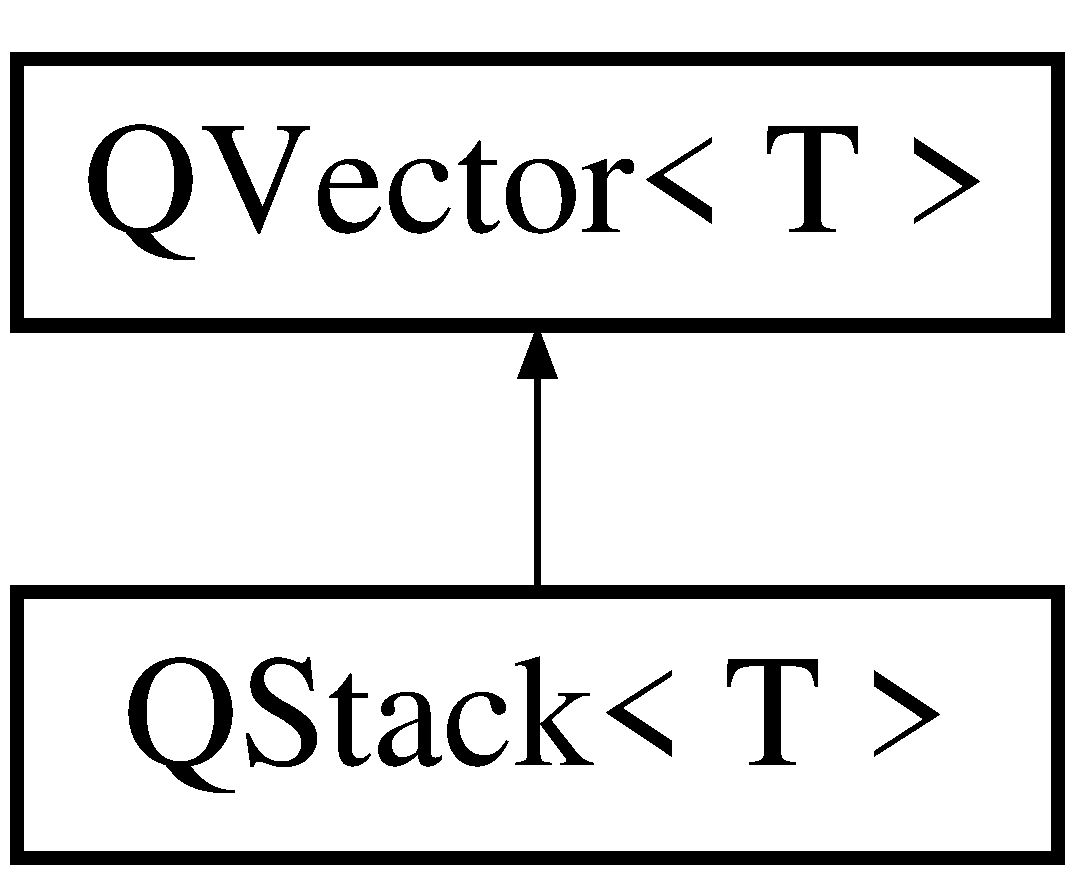
\includegraphics[height=2.000000cm]{class_q_vector}
\end{center}
\end{figure}
\subsection*{Public Types}
\begin{DoxyCompactItemize}
\item 
typedef Data\+::iterator \hyperlink{class_q_vector_af6ac26e0dfede6e3045be0c947201267}{iterator}
\item 
typedef Data\+::const\+\_\+iterator \hyperlink{class_q_vector_a01e19bfad7fefd3e97ef197f4ed2cceb}{const\+\_\+iterator}
\item 
typedef T \hyperlink{class_q_vector_afb003dbc70603eacc89c0c7ea495dd3d}{value\+\_\+type}
\item 
typedef \hyperlink{class_q_vector_afb003dbc70603eacc89c0c7ea495dd3d}{value\+\_\+type} $\ast$ \hyperlink{class_q_vector_ae3fa870723fe1109c22b1091d54075fa}{pointer}
\item 
typedef const \hyperlink{class_q_vector_afb003dbc70603eacc89c0c7ea495dd3d}{value\+\_\+type} $\ast$ \hyperlink{class_q_vector_aa5e3dc32b0a887d59bf5c5c30c95eb85}{const\+\_\+pointer}
\item 
typedef \hyperlink{class_q_vector_afb003dbc70603eacc89c0c7ea495dd3d}{value\+\_\+type} \& \hyperlink{class_q_vector_a86d1c26fb98028474e556d2e25b60633}{reference}
\item 
typedef const \hyperlink{class_q_vector_afb003dbc70603eacc89c0c7ea495dd3d}{value\+\_\+type} \& \hyperlink{class_q_vector_a4054473292677d3bc7d901db7b3b3f20}{const\+\_\+reference}
\item 
typedef qptrdiff \hyperlink{class_q_vector_aaccc790d3ba04fc52580cdfc9d9290fa}{difference\+\_\+type}
\item 
typedef \hyperlink{class_q_vector_af6ac26e0dfede6e3045be0c947201267}{iterator} \hyperlink{class_q_vector_a22a5801860ee27fedc7dca5062355089}{Iterator}
\item 
typedef \hyperlink{class_q_vector_a01e19bfad7fefd3e97ef197f4ed2cceb}{const\+\_\+iterator} \hyperlink{class_q_vector_a480cfc218d799ecba92075c848e605c6}{Const\+Iterator}
\item 
typedef int \hyperlink{class_q_vector_afd8d3d4bf5a63a0c92128507dee59282}{size\+\_\+type}
\end{DoxyCompactItemize}
\subsection*{Public Member Functions}
\begin{DoxyCompactItemize}
\item 
\hyperlink{class_q_vector_a93e8a3fa9e7f4934e5f97494ad17f518}{Q\+Vector} () Q\+\_\+\+D\+E\+C\+L\+\_\+\+N\+O\+T\+H\+R\+OW
\item 
\hyperlink{class_q_vector_a000f527522e85e6682807ff7edd9467f}{Q\+Vector} (int \hyperlink{class_q_vector_aa5739a6bcb52f9b9532ac661cca45b8b}{size})
\item 
\hyperlink{class_q_vector_a2c9d422d62125b04a4835de82666e9f2}{Q\+Vector} (int \hyperlink{class_q_vector_aa5739a6bcb52f9b9532ac661cca45b8b}{size}, const T \&t)
\item 
\hyperlink{class_q_vector_a58c57c94049f372ea119f2b0c60fc357}{Q\+Vector} (const \hyperlink{class_q_vector}{Q\+Vector}$<$ T $>$ \&v)
\item 
\hyperlink{class_q_vector_ada8501475bf1f9eb3e1aa6d70c84b79c}{$\sim$\+Q\+Vector} ()
\item 
\hyperlink{class_q_vector}{Q\+Vector}$<$ T $>$ \& \hyperlink{class_q_vector_a36236603096c0c02def1c0d43f3ebbf5}{operator=} (const \hyperlink{class_q_vector}{Q\+Vector}$<$ T $>$ \&v)
\item 
void \hyperlink{class_q_vector_a35254d6c26569b985958b2ed15695fb6}{swap} (\hyperlink{class_q_vector}{Q\+Vector}$<$ T $>$ \&other)
\item 
bool \hyperlink{class_q_vector_a4d4ee275a13de28d0da7e49085ba7a7d}{operator==} (const \hyperlink{class_q_vector}{Q\+Vector}$<$ T $>$ \&v) const 
\item 
bool \hyperlink{class_q_vector_a7c3c88c0f770426a9b9dbb77ba1dcbfe}{operator!=} (const \hyperlink{class_q_vector}{Q\+Vector}$<$ T $>$ \&v) const 
\item 
int \hyperlink{class_q_vector_aa5739a6bcb52f9b9532ac661cca45b8b}{size} () const 
\item 
bool \hyperlink{class_q_vector_a23ddd6fbfe38f8c34f69b5af89e97000}{is\+Empty} () const 
\item 
void \hyperlink{class_q_vector_a12d291b2dda474720c33a97bfe1b0973}{resize} (int \hyperlink{class_q_vector_aa5739a6bcb52f9b9532ac661cca45b8b}{size})
\item 
int \hyperlink{class_q_vector_a160560e2aab0840e0de275ae9ca48f7a}{capacity} () const 
\item 
void \hyperlink{class_q_vector_aab71cce382721d176d1445434ae18e6a}{reserve} (int \hyperlink{class_q_vector_aa5739a6bcb52f9b9532ac661cca45b8b}{size})
\item 
void \hyperlink{class_q_vector_a8e0d583fe677dad6afd11ed4bc8b8927}{squeeze} ()
\item 
void \hyperlink{class_q_vector_a08d0d1da157ccc4b3de98ac618fab8e6}{detach} ()
\item 
bool \hyperlink{class_q_vector_af229e85b6aa5891a437b3efde705ceea}{is\+Detached} () const 
\item 
bool \hyperlink{class_q_vector_a05ceccc2b7cc2bebfcd9e05ee9406a0e}{is\+Shared\+With} (const \hyperlink{class_q_vector}{Q\+Vector}$<$ T $>$ \&other) const 
\item 
T $\ast$ \hyperlink{class_q_vector_acc8068ddfe8bc93852558914a5e73b5a}{data} ()
\item 
const T $\ast$ \hyperlink{class_q_vector_a0170fb9ced08d46ad0724049a1b7d680}{data} () const 
\item 
const T $\ast$ \hyperlink{class_q_vector_a598509c9fe544e8a47e375f47b5c8f50}{const\+Data} () const 
\item 
void \hyperlink{class_q_vector_a4ec0b396f1d5138386800318ca7d3a0d}{clear} ()
\item 
const T \& \hyperlink{class_q_vector_ab97dbaa9b950ec9c3f3ac51bb602235c}{at} (int i) const 
\item 
T \& \hyperlink{class_q_vector_a145585285bf96d5fcd8ce10f7bc6ec3e}{operator\mbox{[}$\,$\mbox{]}} (int i)
\item 
const T \& \hyperlink{class_q_vector_a4abb4e10e8ea7bcad4819f21c13711f2}{operator\mbox{[}$\,$\mbox{]}} (int i) const 
\item 
void \hyperlink{class_q_vector_ad3536b6c85748f8b0b376d5d9ba0e721}{append} (const T \&t)
\item 
void \hyperlink{class_q_vector_a35a429cf3858d3c58246229b2cc18e93}{append} (const \hyperlink{class_q_vector}{Q\+Vector}$<$ T $>$ \&l)
\item 
void \hyperlink{class_q_vector_a94da89ec9a0c1b5205065ecf08ec1a7d}{prepend} (const T \&t)
\item 
void \hyperlink{class_q_vector_a8567b12d7fa5d23de69ba87e27646ee5}{insert} (int i, const T \&t)
\item 
void \hyperlink{class_q_vector_afb2c6bd6b45f3ce73f4c6556d492af53}{insert} (int i, int n, const T \&t)
\item 
void \hyperlink{class_q_vector_a488cf341031679a18361c89111794059}{replace} (int i, const T \&t)
\item 
void \hyperlink{class_q_vector_a795fabfd2431ce0878ff4ba3c06e7e2b}{remove} (int i)
\item 
void \hyperlink{class_q_vector_aea3b154a0eaf41cb19cf9a916e426a33}{remove} (int i, int n)
\item 
void \hyperlink{class_q_vector_a93907fcd36758247f6d6e074240f9f02}{remove\+First} ()
\item 
void \hyperlink{class_q_vector_a601a6ef4768c988b5ce96e05a8449f64}{remove\+Last} ()
\item 
T \hyperlink{class_q_vector_a96a07a40f38b70e6c71fc3f01749636b}{take\+First} ()
\item 
T \hyperlink{class_q_vector_a81212706ea7a741742d342d0c370a783}{take\+Last} ()
\item 
\hyperlink{class_q_vector}{Q\+Vector}$<$ T $>$ \& \hyperlink{class_q_vector_aa508b6403bbbe6f81b67d0c9257b7d2b}{fill} (const T \&t, int \hyperlink{class_q_vector_aa5739a6bcb52f9b9532ac661cca45b8b}{size}=-\/1)
\item 
int \hyperlink{class_q_vector_a015c576d25fc9707466b3b301e10f33d}{index\+Of} (const T \&t, int from=0) const 
\item 
int \hyperlink{class_q_vector_a06149e241b9907f6c2b379c4e5279338}{last\+Index\+Of} (const T \&t, int from=-\/1) const 
\item 
bool \hyperlink{class_q_vector_a048b668c8baf8e2503656a751e73ddad}{contains} (const T \&t) const 
\item 
int \hyperlink{class_q_vector_a0ba5f2f633ab9eb813e6433464f095a6}{count} (const T \&t) const 
\item 
void \hyperlink{class_q_vector_a33bedda19185b72dcaa008f52ddd3ed0}{remove\+At} (int i)
\item 
int \hyperlink{class_q_vector_aa78630cc416f99d5d1984ea402da9516}{remove\+All} (const T \&t)
\item 
bool \hyperlink{class_q_vector_aae46c554ac81f614f376425cef90149d}{remove\+One} (const T \&t)
\item 
int \hyperlink{class_q_vector_a44cb545af1984e4c9432b0cc57525664}{length} () const 
\item 
T \hyperlink{class_q_vector_a47372e861a3e52af5d2ea6ee29bc5de0}{take\+At} (int i)
\item 
\hyperlink{class_q_vector_af6ac26e0dfede6e3045be0c947201267}{iterator} \hyperlink{class_q_vector_ad0c2c0e80b789c3a78a8c3a32dba31cc}{begin} ()
\item 
\hyperlink{class_q_vector_a01e19bfad7fefd3e97ef197f4ed2cceb}{const\+\_\+iterator} \hyperlink{class_q_vector_af4315069a3caf05631993ec7d57881fa}{begin} () const 
\item 
\hyperlink{class_q_vector_a01e19bfad7fefd3e97ef197f4ed2cceb}{const\+\_\+iterator} \hyperlink{class_q_vector_a4ccddab5fdd95438143d5dbb17afc404}{cbegin} () const 
\item 
\hyperlink{class_q_vector_a01e19bfad7fefd3e97ef197f4ed2cceb}{const\+\_\+iterator} \hyperlink{class_q_vector_a8f2ae9da9b4f929a1cbb718e2ff1a9ca}{const\+Begin} () const 
\item 
\hyperlink{class_q_vector_af6ac26e0dfede6e3045be0c947201267}{iterator} \hyperlink{class_q_vector_aee13fe5819dcac8aee22f40f31c2790b}{end} ()
\item 
\hyperlink{class_q_vector_a01e19bfad7fefd3e97ef197f4ed2cceb}{const\+\_\+iterator} \hyperlink{class_q_vector_ad13adb8ee2256f8b583509d7d9c4ca44}{end} () const 
\item 
\hyperlink{class_q_vector_a01e19bfad7fefd3e97ef197f4ed2cceb}{const\+\_\+iterator} \hyperlink{class_q_vector_aae87e757422aae4f12f8b8b60b2efb19}{cend} () const 
\item 
\hyperlink{class_q_vector_a01e19bfad7fefd3e97ef197f4ed2cceb}{const\+\_\+iterator} \hyperlink{class_q_vector_a86b54d84b2435c97d8ec62d5149eeee8}{const\+End} () const 
\item 
\hyperlink{class_q_vector_af6ac26e0dfede6e3045be0c947201267}{iterator} \hyperlink{class_q_vector_a85e9511cdd9b7949828749a8092af924}{insert} (\hyperlink{class_q_vector_af6ac26e0dfede6e3045be0c947201267}{iterator} before, int n, const T \&x)
\item 
\hyperlink{class_q_vector_af6ac26e0dfede6e3045be0c947201267}{iterator} \hyperlink{class_q_vector_acb1662d362fcf2fcc2ae820d08fd159d}{insert} (\hyperlink{class_q_vector_af6ac26e0dfede6e3045be0c947201267}{iterator} before, const T \&x)
\item 
\hyperlink{class_q_vector_af6ac26e0dfede6e3045be0c947201267}{iterator} \hyperlink{class_q_vector_af58c46c4f0db158717e382fe894c1484}{erase} (\hyperlink{class_q_vector_af6ac26e0dfede6e3045be0c947201267}{iterator} \hyperlink{class_q_vector_ad0c2c0e80b789c3a78a8c3a32dba31cc}{begin}, \hyperlink{class_q_vector_af6ac26e0dfede6e3045be0c947201267}{iterator} \hyperlink{class_q_vector_aee13fe5819dcac8aee22f40f31c2790b}{end})
\item 
\hyperlink{class_q_vector_af6ac26e0dfede6e3045be0c947201267}{iterator} \hyperlink{class_q_vector_a86403f70f137b660c6750f2b37c1e7d0}{erase} (\hyperlink{class_q_vector_af6ac26e0dfede6e3045be0c947201267}{iterator} pos)
\item 
int \hyperlink{class_q_vector_a7523e0dd8ab0759ad53b32d18da10780}{count} () const 
\item 
T \& \hyperlink{class_q_vector_a85cff791949dfb35bc432c6c5afae966}{first} ()
\item 
const T \& \hyperlink{class_q_vector_ac9e38c34b78e0460d7f19713d5588e7d}{first} () const 
\item 
T \& \hyperlink{class_q_vector_a93f335707c6d1003dd2b594e4066ed0b}{last} ()
\item 
const T \& \hyperlink{class_q_vector_a200d93e8b761b606c07f86fe4be44cef}{last} () const 
\item 
bool \hyperlink{class_q_vector_a264d1d6641f51e6fe2bbd1fdb1e93528}{starts\+With} (const T \&t) const 
\item 
bool \hyperlink{class_q_vector_a166cfa66c83c7255127a40ad26773a99}{ends\+With} (const T \&t) const 
\item 
\hyperlink{class_q_vector}{Q\+Vector}$<$ T $>$ \hyperlink{class_q_vector_a09c185dcd5d2f02fd05dd4db84be1d28}{mid} (int pos, int len=-\/1) const 
\item 
T \hyperlink{class_q_vector_a3788cd97b1cd4898d508422cb1227f8c}{value} (int i) const 
\item 
T \hyperlink{class_q_vector_a6e81cced2857ea1d3bd3eb5eb90fe527}{value} (int i, const T \&default\+Value) const 
\item 
void \hyperlink{class_q_vector_a64a78ac295cf7c41fde971c9811116a9}{push\+\_\+back} (const T \&t)
\item 
void \hyperlink{class_q_vector_a6d51ebc0e8ff3ee57ac13170086827a5}{push\+\_\+front} (const T \&t)
\item 
void \hyperlink{class_q_vector_a4e4045d36b19dc7a6b8e3893f27f2b99}{pop\+\_\+back} ()
\item 
void \hyperlink{class_q_vector_aabe2aff9d7f1496d37d04c50e3741d0e}{pop\+\_\+front} ()
\item 
bool \hyperlink{class_q_vector_a07249d8a8b0eade3f37104ae0357d0bf}{empty} () const 
\item 
T \& \hyperlink{class_q_vector_a479198a1d185e0191e1170c200bb74aa}{front} ()
\item 
\hyperlink{class_q_vector_a4054473292677d3bc7d901db7b3b3f20}{const\+\_\+reference} \hyperlink{class_q_vector_a402094ad8fe1fe7ead5d6217466da3bc}{front} () const 
\item 
\hyperlink{class_q_vector_a86d1c26fb98028474e556d2e25b60633}{reference} \hyperlink{class_q_vector_abbea52a372bdc71b374acb422e4a4ce0}{back} ()
\item 
\hyperlink{class_q_vector_a4054473292677d3bc7d901db7b3b3f20}{const\+\_\+reference} \hyperlink{class_q_vector_a0bb36e8f88a033d56d422f6b65c29465}{back} () const 
\item 
\hyperlink{class_q_vector}{Q\+Vector}$<$ T $>$ \& \hyperlink{class_q_vector_add550c8dd5120227c645ecb069cb7196}{operator+=} (const \hyperlink{class_q_vector}{Q\+Vector}$<$ T $>$ \&l)
\item 
\hyperlink{class_q_vector}{Q\+Vector}$<$ T $>$ \hyperlink{class_q_vector_a8f2255fa151633ab15cd46a1ea9d8bf1}{operator+} (const \hyperlink{class_q_vector}{Q\+Vector}$<$ T $>$ \&l) const 
\item 
\hyperlink{class_q_vector}{Q\+Vector}$<$ T $>$ \& \hyperlink{class_q_vector_a7597c1f0f004594f8e446bb6ae09601c}{operator+=} (const T \&t)
\item 
\hyperlink{class_q_vector}{Q\+Vector}$<$ T $>$ \& \hyperlink{class_q_vector_a60144939301f38042c9f702ae887ea16}{operator$<$$<$} (const T \&t)
\item 
\hyperlink{class_q_vector}{Q\+Vector}$<$ T $>$ \& \hyperlink{class_q_vector_a36aa335f06fab320bc322cb817808a34}{operator$<$$<$} (const \hyperlink{class_q_vector}{Q\+Vector}$<$ T $>$ \&l)
\item 
\hyperlink{class_q_list}{Q\+List}$<$ T $>$ \hyperlink{class_q_vector_a604c990aa7914fc3840c740b4bb0ff7d}{to\+List} () const 
\item 
std\+::vector$<$ T $>$ \hyperlink{class_q_vector_a0bb56bf3c3e5c533efda20ff4394b444}{to\+Std\+Vector} () const 
\end{DoxyCompactItemize}
\subsection*{Static Public Member Functions}
\begin{DoxyCompactItemize}
\item 
static \hyperlink{class_q_vector}{Q\+Vector}$<$ T $>$ \hyperlink{class_q_vector_a81688755b0166749fde54c1108690825}{from\+List} (const \hyperlink{class_q_list}{Q\+List}$<$ T $>$ \&list)
\item 
static \hyperlink{class_q_vector}{Q\+Vector}$<$ T $>$ \hyperlink{class_q_vector_a4bb034c193b1f443b235df30323ee2d0}{from\+Std\+Vector} (const std\+::vector$<$ T $>$ \&vector)
\end{DoxyCompactItemize}
\subsection*{Friends}
\begin{DoxyCompactItemize}
\item 
class \hyperlink{class_q_vector_a3c463c91639ee085a365c4bf70fcbe31}{Q\+Region}
\end{DoxyCompactItemize}
\subsection*{Related Functions}
(Note that these are not member functions.) \begin{DoxyCompactItemize}
\item 
Q\+Data\+Stream \& \hyperlink{class_q_vector_a556a703e2a1987feda15598f2d097d34}{operator$<$$<$} (Q\+Data\+Stream \&out, const \hyperlink{class_q_vector}{Q\+Vector}$<$ T $>$ \&vector)
\item 
Q\+Data\+Stream \& \hyperlink{class_q_vector_aa3718549b9b553556b654f6e00aaa914}{operator$>$$>$} (Q\+Data\+Stream \&in, \hyperlink{class_q_vector}{Q\+Vector}$<$ T $>$ \&vector)
\end{DoxyCompactItemize}


\subsection{Detailed Description}
\subsubsection*{template$<$typename T$>$\\*
class Q\+Vector$<$ T $>$}

The \hyperlink{class_q_vector}{Q\+Vector} class is a template class that provides a dynamic array. 

Qt\+Core

\hyperlink{class_q_vector}{Q\+Vector}$<$T$>$ is one of Qt\textquotesingle{}s generic \{container classes\}. It stores its items in adjacent memory locations and provides fast index-\/based access.

\hyperlink{class_q_list}{Q\+List}$<$T$>$, Q\+Linked\+List$<$T$>$, and Q\+Var\+Length\+Array$<$T$>$ provide similar functionality. Here\textquotesingle{}s an overview\+:

\begin{DoxyItemize}
\item For most purposes, \hyperlink{class_q_list}{Q\+List} is the right class to use. Operations like \hyperlink{class_q_vector_a94da89ec9a0c1b5205065ecf08ec1a7d}{prepend()} and \hyperlink{class_q_vector_a8567b12d7fa5d23de69ba87e27646ee5}{insert()} are usually faster than with \hyperlink{class_q_vector}{Q\+Vector} because of the way \hyperlink{class_q_list}{Q\+List} stores its items in memory (see \{Algorithmic Complexity\} for details), and its index-\/based A\+PI is more convenient than Q\+Linked\+List\textquotesingle{}s iterator-\/based A\+PI. It also expands to less code in your executable. \item If you need a real linked list, with guarantees of \{constant time\} insertions in the middle of the list and iterators to items rather than indexes, use Q\+Linked\+List. \item If you want the items to occupy adjacent memory positions, or if your items are larger than a pointer and you want to avoid the overhead of allocating them on the heap individually at insertion time, then use \hyperlink{class_q_vector}{Q\+Vector}. \item If you want a low-\/level variable-\/size array, Q\+Var\+Length\+Array may be sufficient. \end{DoxyItemize}
Here\textquotesingle{}s an example of a \hyperlink{class_q_vector}{Q\+Vector} that stores integers and a \hyperlink{class_q_vector}{Q\+Vector} that stores Q\+String values\+:


\begin{DoxyCodeInclude}
\end{DoxyCodeInclude}
 \hyperlink{class_q_vector}{Q\+Vector} stores a vector (or array) of items. Typically, vectors are created with an initial size. For example, the following code constructs a \hyperlink{class_q_vector}{Q\+Vector} with 200 elements\+:


\begin{DoxyCodeInclude}
\end{DoxyCodeInclude}
 The elements are automatically initialized with a \{default-\/constructed value\}. If you want to initialize the vector with a different value, pass that value as the second argument to the constructor\+:


\begin{DoxyCodeInclude}
\end{DoxyCodeInclude}
 You can also call \hyperlink{class_q_vector_aa508b6403bbbe6f81b67d0c9257b7d2b}{fill()} at any time to fill the vector with a value.

\hyperlink{class_q_vector}{Q\+Vector} uses 0-\/based indexes, just like C++ arrays. To access the item at a particular index position, you can use \hyperlink{class_q_vector_a145585285bf96d5fcd8ce10f7bc6ec3e}{operator\mbox{[}$\,$\mbox{]}()}. On non-\/const vectors, \hyperlink{class_q_vector_a145585285bf96d5fcd8ce10f7bc6ec3e}{operator\mbox{[}$\,$\mbox{]}()} returns a reference to the item that can be used on the left side of an assignment\+:


\begin{DoxyCodeInclude}
\end{DoxyCodeInclude}
 For read-\/only access, an alternative syntax is to use \hyperlink{class_q_vector_ab97dbaa9b950ec9c3f3ac51bb602235c}{at()}\+:


\begin{DoxyCodeInclude}
\end{DoxyCodeInclude}
 \hyperlink{class_q_vector_ab97dbaa9b950ec9c3f3ac51bb602235c}{at()} can be faster than \hyperlink{class_q_vector_a145585285bf96d5fcd8ce10f7bc6ec3e}{operator\mbox{[}$\,$\mbox{]}()}, because it never causes a \{deep copy\} to occur.

Another way to access the data stored in a \hyperlink{class_q_vector}{Q\+Vector} is to call \hyperlink{class_q_vector_acc8068ddfe8bc93852558914a5e73b5a}{data()}. The function returns a pointer to the first item in the vector. You can use the pointer to directly access and modify the elements stored in the vector. The pointer is also useful if you need to pass a \hyperlink{class_q_vector}{Q\+Vector} to a function that accepts a plain C++ array.

If you want to find all occurrences of a particular value in a vector, use \hyperlink{class_q_vector_a015c576d25fc9707466b3b301e10f33d}{index\+Of()} or \hyperlink{class_q_vector_a06149e241b9907f6c2b379c4e5279338}{last\+Index\+Of()}. The former searches forward starting from a given index position, the latter searches backward. Both return the index of the matching item if they found one; otherwise, they return -\/1. For example\+:


\begin{DoxyCodeInclude}
\end{DoxyCodeInclude}
 If you simply want to check whether a vector contains a particular value, use \hyperlink{class_q_vector_a048b668c8baf8e2503656a751e73ddad}{contains()}. If you want to find out how many times a particular value occurs in the vector, use \hyperlink{class_q_vector_a0ba5f2f633ab9eb813e6433464f095a6}{count()}.

\hyperlink{class_q_vector}{Q\+Vector} provides these basic functions to add, move, and remove items\+: \hyperlink{class_q_vector_a8567b12d7fa5d23de69ba87e27646ee5}{insert()}, \hyperlink{class_q_vector_a488cf341031679a18361c89111794059}{replace()}, \hyperlink{class_q_vector_a795fabfd2431ce0878ff4ba3c06e7e2b}{remove()}, \hyperlink{class_q_vector_a94da89ec9a0c1b5205065ecf08ec1a7d}{prepend()}, \hyperlink{class_q_vector_ad3536b6c85748f8b0b376d5d9ba0e721}{append()}. With the exception of \hyperlink{class_q_vector_ad3536b6c85748f8b0b376d5d9ba0e721}{append()} and \hyperlink{class_q_vector_a488cf341031679a18361c89111794059}{replace()}, these functions can be slow (\{linear time\}) for large vectors, because they require moving many items in the vector by one position in memory. If you want a container class that provides fast insertion/removal in the middle, use \hyperlink{class_q_list}{Q\+List} or Q\+Linked\+List instead.

Unlike plain C++ arrays, Q\+Vectors can be resized at any time by calling \hyperlink{class_q_vector_a12d291b2dda474720c33a97bfe1b0973}{resize()}. If the new size is larger than the old size, \hyperlink{class_q_vector}{Q\+Vector} might need to reallocate the whole vector. \hyperlink{class_q_vector}{Q\+Vector} tries to reduce the number of reallocations by preallocating up to twice as much memory as the actual data needs.

If you know in advance approximately how many items the \hyperlink{class_q_vector}{Q\+Vector} will contain, you can call \hyperlink{class_q_vector_aab71cce382721d176d1445434ae18e6a}{reserve()}, asking \hyperlink{class_q_vector}{Q\+Vector} to preallocate a certain amount of memory. You can also call \hyperlink{class_q_vector_a160560e2aab0840e0de275ae9ca48f7a}{capacity()} to find out how much memory \hyperlink{class_q_vector}{Q\+Vector} actually allocated.

Note that using non-\/const operators and functions can cause \hyperlink{class_q_vector}{Q\+Vector} to do a deep copy of the data. This is due to \{implicit sharing\}.

\hyperlink{class_q_vector}{Q\+Vector}\textquotesingle{}s value type must be an \{assignable data type\}. This covers most data types that are commonly used, but the compiler won\textquotesingle{}t let you, for example, store a Q\+Widget as a value; instead, store a Q\+Widget $\ast$. A few functions have additional requirements; for example, \hyperlink{class_q_vector_a015c576d25fc9707466b3b301e10f33d}{index\+Of()} and \hyperlink{class_q_vector_a06149e241b9907f6c2b379c4e5279338}{last\+Index\+Of()} expect the value type to support {\ttfamily \hyperlink{class_q_vector_a4d4ee275a13de28d0da7e49085ba7a7d}{operator==()}}. These requirements are documented on a per-\/function basis.

Like the other container classes, \hyperlink{class_q_vector}{Q\+Vector} provides \{Java-\/style iterators\} (Q\+Vector\+Iterator and Q\+Mutable\+Vector\+Iterator) and \{S\+T\+L-\/style iterators\} (\hyperlink{class_q_vector_a01e19bfad7fefd3e97ef197f4ed2cceb}{Q\+Vector\+::const\+\_\+iterator} and \hyperlink{class_q_vector_af6ac26e0dfede6e3045be0c947201267}{Q\+Vector\+::iterator}). In practice, these are rarely used, because you can use indexes into the \hyperlink{class_q_vector}{Q\+Vector}.

In addition to \hyperlink{class_q_vector}{Q\+Vector}, Qt also provides Q\+Var\+Length\+Array, a very low-\/level class with little functionality that is optimized for speed.

\hyperlink{class_q_vector}{Q\+Vector} does {\itshape not} support inserting, prepending, appending or replacing with references to its own values. Doing so will cause your application to abort with an error message.

\begin{DoxySeeAlso}{See also}
Q\+Vector\+Iterator, Q\+Mutable\+Vector\+Iterator, \hyperlink{class_q_list}{Q\+List}, Q\+Linked\+List 
\end{DoxySeeAlso}


Definition at line 62 of file qlist.\+h.



\subsection{Member Typedef Documentation}
\index{Q\+Vector@{Q\+Vector}!const\+\_\+iterator@{const\+\_\+iterator}}
\index{const\+\_\+iterator@{const\+\_\+iterator}!Q\+Vector@{Q\+Vector}}
\subsubsection[{\texorpdfstring{const\+\_\+iterator}{const_iterator}}]{\setlength{\rightskip}{0pt plus 5cm}template$<$typename T$>$ {\bf Q\+Vector}$<$ T $>$\+::{\bf const\+\_\+iterator}}\hypertarget{class_q_vector_a01e19bfad7fefd3e97ef197f4ed2cceb}{}\label{class_q_vector_a01e19bfad7fefd3e97ef197f4ed2cceb}
The \hyperlink{class_q_vector_a01e19bfad7fefd3e97ef197f4ed2cceb}{Q\+Vector\+::const\+\_\+iterator} typedef provides an S\+T\+L-\/style const iterator for \hyperlink{class_q_vector}{Q\+Vector} and \hyperlink{class_q_stack}{Q\+Stack}.

\hyperlink{class_q_vector}{Q\+Vector} provides both \{S\+T\+L-\/style iterators\} and \{Java-\/style iterators\}. The S\+T\+L-\/style const iterator is simply a typedef for \char`\"{}const T $\ast$\char`\"{} (pointer to const T).

\begin{DoxyWarning}{Warning}
Iterators on implicitly shared containers do not work exactly like S\+T\+L-\/iterators. You should avoid copying a container while iterators are active on that container. For more information, read \{Implicit sharing iterator problem\}.
\end{DoxyWarning}
\begin{DoxySeeAlso}{See also}
\hyperlink{class_q_vector_a8f2ae9da9b4f929a1cbb718e2ff1a9ca}{Q\+Vector\+::const\+Begin()}, \hyperlink{class_q_vector_a86b54d84b2435c97d8ec62d5149eeee8}{Q\+Vector\+::const\+End()}, \hyperlink{class_q_vector_af6ac26e0dfede6e3045be0c947201267}{Q\+Vector\+::iterator}, Q\+Vector\+Iterator 
\end{DoxySeeAlso}


Definition at line 177 of file qvector.\+h.

\index{Q\+Vector@{Q\+Vector}!const\+\_\+pointer@{const\+\_\+pointer}}
\index{const\+\_\+pointer@{const\+\_\+pointer}!Q\+Vector@{Q\+Vector}}
\subsubsection[{\texorpdfstring{const\+\_\+pointer}{const_pointer}}]{\setlength{\rightskip}{0pt plus 5cm}template$<$typename T$>$ {\bf Q\+Vector}$<$ T $>$\+::{\bf const\+\_\+pointer}}\hypertarget{class_q_vector_aa5e3dc32b0a887d59bf5c5c30c95eb85}{}\label{class_q_vector_aa5e3dc32b0a887d59bf5c5c30c95eb85}
Typedef for const T $\ast$. Provided for S\+TL compatibility. 

Definition at line 218 of file qvector.\+h.

\index{Q\+Vector@{Q\+Vector}!const\+\_\+reference@{const\+\_\+reference}}
\index{const\+\_\+reference@{const\+\_\+reference}!Q\+Vector@{Q\+Vector}}
\subsubsection[{\texorpdfstring{const\+\_\+reference}{const_reference}}]{\setlength{\rightskip}{0pt plus 5cm}template$<$typename T$>$ {\bf Q\+Vector}$<$ T $>$\+::{\bf const\+\_\+reference}}\hypertarget{class_q_vector_a4054473292677d3bc7d901db7b3b3f20}{}\label{class_q_vector_a4054473292677d3bc7d901db7b3b3f20}
Typedef for T \&. Provided for S\+TL compatibility. 

Definition at line 220 of file qvector.\+h.

\index{Q\+Vector@{Q\+Vector}!Const\+Iterator@{Const\+Iterator}}
\index{Const\+Iterator@{Const\+Iterator}!Q\+Vector@{Q\+Vector}}
\subsubsection[{\texorpdfstring{Const\+Iterator}{ConstIterator}}]{\setlength{\rightskip}{0pt plus 5cm}template$<$typename T$>$ {\bf Q\+Vector}$<$ T $>$\+::{\bf Const\+Iterator}}\hypertarget{class_q_vector_a480cfc218d799ecba92075c848e605c6}{}\label{class_q_vector_a480cfc218d799ecba92075c848e605c6}
Qt-\/style synonym for \hyperlink{class_q_vector_a01e19bfad7fefd3e97ef197f4ed2cceb}{Q\+Vector\+::const\+\_\+iterator}. 

Definition at line 223 of file qvector.\+h.

\index{Q\+Vector@{Q\+Vector}!difference\+\_\+type@{difference\+\_\+type}}
\index{difference\+\_\+type@{difference\+\_\+type}!Q\+Vector@{Q\+Vector}}
\subsubsection[{\texorpdfstring{difference\+\_\+type}{difference_type}}]{\setlength{\rightskip}{0pt plus 5cm}template$<$typename T$>$ {\bf Q\+Vector}$<$ T $>$\+::{\bf difference\+\_\+type}}\hypertarget{class_q_vector_aaccc790d3ba04fc52580cdfc9d9290fa}{}\label{class_q_vector_aaccc790d3ba04fc52580cdfc9d9290fa}
Typedef for ptrdiff\+\_\+t. Provided for S\+TL compatibility. 

Definition at line 221 of file qvector.\+h.

\index{Q\+Vector@{Q\+Vector}!iterator@{iterator}}
\index{iterator@{iterator}!Q\+Vector@{Q\+Vector}}
\subsubsection[{\texorpdfstring{iterator}{iterator}}]{\setlength{\rightskip}{0pt plus 5cm}template$<$typename T$>$ {\bf Q\+Vector}$<$ T $>$\+::{\bf iterator}}\hypertarget{class_q_vector_af6ac26e0dfede6e3045be0c947201267}{}\label{class_q_vector_af6ac26e0dfede6e3045be0c947201267}
The \hyperlink{class_q_vector_af6ac26e0dfede6e3045be0c947201267}{Q\+Vector\+::iterator} typedef provides an S\+T\+L-\/style non-\/const iterator for \hyperlink{class_q_vector}{Q\+Vector} and \hyperlink{class_q_stack}{Q\+Stack}.

\hyperlink{class_q_vector}{Q\+Vector} provides both \{S\+T\+L-\/style iterators\} and \{Java-\/style iterators\}. The S\+T\+L-\/style non-\/const iterator is simply a typedef for \char`\"{}\+T $\ast$\char`\"{} (pointer to T).

\begin{DoxyWarning}{Warning}
Iterators on implicitly shared containers do not work exactly like S\+T\+L-\/iterators. You should avoid copying a container while iterators are active on that container. For more information, read \{Implicit sharing iterator problem\}.
\end{DoxyWarning}
\begin{DoxySeeAlso}{See also}
\hyperlink{class_q_vector_ad0c2c0e80b789c3a78a8c3a32dba31cc}{Q\+Vector\+::begin()}, \hyperlink{class_q_vector_aee13fe5819dcac8aee22f40f31c2790b}{Q\+Vector\+::end()}, \hyperlink{class_q_vector_a01e19bfad7fefd3e97ef197f4ed2cceb}{Q\+Vector\+::const\+\_\+iterator}, Q\+Mutable\+Vector\+Iterator 
\end{DoxySeeAlso}


Definition at line 176 of file qvector.\+h.

\index{Q\+Vector@{Q\+Vector}!Iterator@{Iterator}}
\index{Iterator@{Iterator}!Q\+Vector@{Q\+Vector}}
\subsubsection[{\texorpdfstring{Iterator}{Iterator}}]{\setlength{\rightskip}{0pt plus 5cm}template$<$typename T$>$ {\bf Q\+Vector}$<$ T $>$\+::{\bf Iterator}}\hypertarget{class_q_vector_a22a5801860ee27fedc7dca5062355089}{}\label{class_q_vector_a22a5801860ee27fedc7dca5062355089}
Qt-\/style synonym for \hyperlink{class_q_vector_af6ac26e0dfede6e3045be0c947201267}{Q\+Vector\+::iterator}. 

Definition at line 222 of file qvector.\+h.

\index{Q\+Vector@{Q\+Vector}!pointer@{pointer}}
\index{pointer@{pointer}!Q\+Vector@{Q\+Vector}}
\subsubsection[{\texorpdfstring{pointer}{pointer}}]{\setlength{\rightskip}{0pt plus 5cm}template$<$typename T$>$ {\bf Q\+Vector}$<$ T $>$\+::{\bf pointer}}\hypertarget{class_q_vector_ae3fa870723fe1109c22b1091d54075fa}{}\label{class_q_vector_ae3fa870723fe1109c22b1091d54075fa}
Typedef for T $\ast$. Provided for S\+TL compatibility. 

Definition at line 217 of file qvector.\+h.

\index{Q\+Vector@{Q\+Vector}!reference@{reference}}
\index{reference@{reference}!Q\+Vector@{Q\+Vector}}
\subsubsection[{\texorpdfstring{reference}{reference}}]{\setlength{\rightskip}{0pt plus 5cm}template$<$typename T$>$ {\bf Q\+Vector}$<$ T $>$\+::{\bf reference}}\hypertarget{class_q_vector_a86d1c26fb98028474e556d2e25b60633}{}\label{class_q_vector_a86d1c26fb98028474e556d2e25b60633}
Typedef for T \&. Provided for S\+TL compatibility. 

Definition at line 219 of file qvector.\+h.

\index{Q\+Vector@{Q\+Vector}!size\+\_\+type@{size\+\_\+type}}
\index{size\+\_\+type@{size\+\_\+type}!Q\+Vector@{Q\+Vector}}
\subsubsection[{\texorpdfstring{size\+\_\+type}{size_type}}]{\setlength{\rightskip}{0pt plus 5cm}template$<$typename T$>$ {\bf Q\+Vector}$<$ T $>$\+::{\bf size\+\_\+type}}\hypertarget{class_q_vector_afd8d3d4bf5a63a0c92128507dee59282}{}\label{class_q_vector_afd8d3d4bf5a63a0c92128507dee59282}
Typedef for int. Provided for S\+TL compatibility. 

Definition at line 224 of file qvector.\+h.

\index{Q\+Vector@{Q\+Vector}!value\+\_\+type@{value\+\_\+type}}
\index{value\+\_\+type@{value\+\_\+type}!Q\+Vector@{Q\+Vector}}
\subsubsection[{\texorpdfstring{value\+\_\+type}{value_type}}]{\setlength{\rightskip}{0pt plus 5cm}template$<$typename T$>$ {\bf Q\+Vector}$<$ T $>$\+::{\bf value\+\_\+type}}\hypertarget{class_q_vector_afb003dbc70603eacc89c0c7ea495dd3d}{}\label{class_q_vector_afb003dbc70603eacc89c0c7ea495dd3d}
Typedef for T. Provided for S\+TL compatibility. 

Definition at line 216 of file qvector.\+h.



\subsection{Constructor \& Destructor Documentation}
\index{Q\+Vector@{Q\+Vector}!Q\+Vector@{Q\+Vector}}
\index{Q\+Vector@{Q\+Vector}!Q\+Vector@{Q\+Vector}}
\subsubsection[{\texorpdfstring{Q\+Vector() Q\+\_\+\+D\+E\+C\+L\+\_\+\+N\+O\+T\+H\+R\+OW}{QVector() Q_DECL_NOTHROW}}]{\setlength{\rightskip}{0pt plus 5cm}template$<$typename T$>$ {\bf Q\+Vector}$<$ T $>$\+::{\bf Q\+Vector} (
\begin{DoxyParamCaption}
{}
\end{DoxyParamCaption}
)\hspace{0.3cm}{\ttfamily [inline]}}\hypertarget{class_q_vector_a93e8a3fa9e7f4934e5f97494ad17f518}{}\label{class_q_vector_a93e8a3fa9e7f4934e5f97494ad17f518}
Constructs an empty vector.

\begin{DoxySeeAlso}{See also}
\hyperlink{class_q_vector_a12d291b2dda474720c33a97bfe1b0973}{resize()} 
\end{DoxySeeAlso}


Definition at line 64 of file qvector.\+h.

\index{Q\+Vector@{Q\+Vector}!Q\+Vector@{Q\+Vector}}
\index{Q\+Vector@{Q\+Vector}!Q\+Vector@{Q\+Vector}}
\subsubsection[{\texorpdfstring{Q\+Vector(int size)}{QVector(int size)}}]{\setlength{\rightskip}{0pt plus 5cm}template$<$typename T $>$ {\bf Q\+Vector}$<$ T $>$\+::{\bf Q\+Vector} (
\begin{DoxyParamCaption}
\item[{int}]{size}
\end{DoxyParamCaption}
)\hspace{0.3cm}{\ttfamily [explicit]}}\hypertarget{class_q_vector_a000f527522e85e6682807ff7edd9467f}{}\label{class_q_vector_a000f527522e85e6682807ff7edd9467f}
Constructs a vector with an initial size of {\itshape size} elements.

The elements are initialized with a \{default-\/constructed value\}.

\begin{DoxySeeAlso}{See also}
\hyperlink{class_q_vector_a12d291b2dda474720c33a97bfe1b0973}{resize()} 
\end{DoxySeeAlso}


Definition at line 442 of file qvector.\+h.

\index{Q\+Vector@{Q\+Vector}!Q\+Vector@{Q\+Vector}}
\index{Q\+Vector@{Q\+Vector}!Q\+Vector@{Q\+Vector}}
\subsubsection[{\texorpdfstring{Q\+Vector(int size, const T \&t)}{QVector(int size, const T &t)}}]{\setlength{\rightskip}{0pt plus 5cm}template$<$typename T$>$ {\bf Q\+Vector}$<$ T $>$\+::{\bf Q\+Vector} (
\begin{DoxyParamCaption}
\item[{int}]{size, }
\item[{const T \&}]{value}
\end{DoxyParamCaption}
)}\hypertarget{class_q_vector_a2c9d422d62125b04a4835de82666e9f2}{}\label{class_q_vector_a2c9d422d62125b04a4835de82666e9f2}
Constructs a vector with an initial size of {\itshape size} elements. Each element is initialized with {\itshape value}.

\begin{DoxySeeAlso}{See also}
\hyperlink{class_q_vector_a12d291b2dda474720c33a97bfe1b0973}{resize()}, \hyperlink{class_q_vector_aa508b6403bbbe6f81b67d0c9257b7d2b}{fill()} 
\end{DoxySeeAlso}


Definition at line 456 of file qvector.\+h.

\index{Q\+Vector@{Q\+Vector}!Q\+Vector@{Q\+Vector}}
\index{Q\+Vector@{Q\+Vector}!Q\+Vector@{Q\+Vector}}
\subsubsection[{\texorpdfstring{Q\+Vector(const Q\+Vector$<$ T $>$ \&v)}{QVector(const QVector< T > &v)}}]{\setlength{\rightskip}{0pt plus 5cm}template$<$typename T$>$ {\bf Q\+Vector}$<$ T $>$\+::{\bf Q\+Vector} (
\begin{DoxyParamCaption}
\item[{const {\bf Q\+Vector}$<$ T $>$ \&}]{other}
\end{DoxyParamCaption}
)\hspace{0.3cm}{\ttfamily [inline]}}\hypertarget{class_q_vector_a58c57c94049f372ea119f2b0c60fc357}{}\label{class_q_vector_a58c57c94049f372ea119f2b0c60fc357}
Constructs a copy of {\itshape other}.

This operation takes \{constant time\}, because \hyperlink{class_q_vector}{Q\+Vector} is \{implicitly shared\}. This makes returning a \hyperlink{class_q_vector}{Q\+Vector} from a function very fast. If a shared instance is modified, it will be copied (copy-\/on-\/write), and that takes \{linear time\}.

\begin{DoxySeeAlso}{See also}
\hyperlink{class_q_vector_a36236603096c0c02def1c0d43f3ebbf5}{operator=()} 
\end{DoxySeeAlso}


Definition at line 326 of file qvector.\+h.

\index{Q\+Vector@{Q\+Vector}!````~Q\+Vector@{$\sim$\+Q\+Vector}}
\index{````~Q\+Vector@{$\sim$\+Q\+Vector}!Q\+Vector@{Q\+Vector}}
\subsubsection[{\texorpdfstring{$\sim$\+Q\+Vector()}{~QVector()}}]{\setlength{\rightskip}{0pt plus 5cm}template$<$typename T$>$ {\bf Q\+Vector}$<$ T $>$\+::$\sim${\bf Q\+Vector} (
\begin{DoxyParamCaption}
{}
\end{DoxyParamCaption}
)\hspace{0.3cm}{\ttfamily [inline]}}\hypertarget{class_q_vector_ada8501475bf1f9eb3e1aa6d70c84b79c}{}\label{class_q_vector_ada8501475bf1f9eb3e1aa6d70c84b79c}
Destroys the vector. 

Definition at line 68 of file qvector.\+h.



\subsection{Member Function Documentation}
\index{Q\+Vector@{Q\+Vector}!append@{append}}
\index{append@{append}!Q\+Vector@{Q\+Vector}}
\subsubsection[{\texorpdfstring{append(const T \&t)}{append(const T &t)}}]{\setlength{\rightskip}{0pt plus 5cm}template$<$typename T$>$ void {\bf Q\+Vector}$<$ T $>$\+::append (
\begin{DoxyParamCaption}
\item[{const T \&}]{value}
\end{DoxyParamCaption}
)}\hypertarget{class_q_vector_ad3536b6c85748f8b0b376d5d9ba0e721}{}\label{class_q_vector_ad3536b6c85748f8b0b376d5d9ba0e721}
Inserts {\itshape value} at the end of the vector.

Example\+: 
\begin{DoxyCodeInclude}
\end{DoxyCodeInclude}
 This is the same as calling resize(\hyperlink{class_q_vector_aa5739a6bcb52f9b9532ac661cca45b8b}{size()} + 1) and assigning {\itshape value} to the new last element in the vector.

This operation is relatively fast, because \hyperlink{class_q_vector}{Q\+Vector} typically allocates more memory than necessary, so it can grow without reallocating the entire vector each time.

\begin{DoxySeeAlso}{See also}
\hyperlink{class_q_vector_a60144939301f38042c9f702ae887ea16}{operator$<$$<$()}, \hyperlink{class_q_vector_a94da89ec9a0c1b5205065ecf08ec1a7d}{prepend()}, \hyperlink{class_q_vector_a8567b12d7fa5d23de69ba87e27646ee5}{insert()} 
\end{DoxySeeAlso}


Definition at line 601 of file qvector.\+h.

\index{Q\+Vector@{Q\+Vector}!append@{append}}
\index{append@{append}!Q\+Vector@{Q\+Vector}}
\subsubsection[{\texorpdfstring{append(const Q\+Vector$<$ T $>$ \&l)}{append(const QVector< T > &l)}}]{\setlength{\rightskip}{0pt plus 5cm}template$<$typename T$>$ void {\bf Q\+Vector}$<$ T $>$\+::append (
\begin{DoxyParamCaption}
\item[{const {\bf Q\+Vector}$<$ T $>$ \&}]{value}
\end{DoxyParamCaption}
)\hspace{0.3cm}{\ttfamily [inline]}}\hypertarget{class_q_vector_a35a429cf3858d3c58246229b2cc18e93}{}\label{class_q_vector_a35a429cf3858d3c58246229b2cc18e93}
This is an overloaded member function, provided for convenience. It differs from the above function only in what argument(s) it accepts.

\begin{DoxySince}{Since}
5.\+5
\end{DoxySince}
Appends the items of the {\itshape value} vector to this vector.

\begin{DoxySeeAlso}{See also}
\hyperlink{class_q_vector_a60144939301f38042c9f702ae887ea16}{operator$<$$<$()}, \hyperlink{class_q_vector_add550c8dd5120227c645ecb069cb7196}{operator+=()} 
\end{DoxySeeAlso}


Definition at line 131 of file qvector.\+h.

\index{Q\+Vector@{Q\+Vector}!at@{at}}
\index{at@{at}!Q\+Vector@{Q\+Vector}}
\subsubsection[{\texorpdfstring{at(int i) const }{at(int i) const }}]{\setlength{\rightskip}{0pt plus 5cm}template$<$typename T $>$ const T \& {\bf Q\+Vector}$<$ T $>$\+::at (
\begin{DoxyParamCaption}
\item[{int}]{i}
\end{DoxyParamCaption}
) const\hspace{0.3cm}{\ttfamily [inline]}}\hypertarget{class_q_vector_ab97dbaa9b950ec9c3f3ac51bb602235c}{}\label{class_q_vector_ab97dbaa9b950ec9c3f3ac51bb602235c}
Returns the item at index position {\itshape i} in the vector.

{\itshape i} must be a valid index position in the vector (i.\+e., 0 $<$= {\itshape i} $<$ \hyperlink{class_q_vector_aa5739a6bcb52f9b9532ac661cca45b8b}{size()}).

\begin{DoxySeeAlso}{See also}
\hyperlink{class_q_vector_a3788cd97b1cd4898d508422cb1227f8c}{value()}, \hyperlink{class_q_vector_a145585285bf96d5fcd8ce10f7bc6ec3e}{operator\mbox{[}$\,$\mbox{]}()} 
\end{DoxySeeAlso}


Definition at line 392 of file qvector.\+h.

\index{Q\+Vector@{Q\+Vector}!back@{back}}
\index{back@{back}!Q\+Vector@{Q\+Vector}}
\subsubsection[{\texorpdfstring{back()}{back()}}]{\setlength{\rightskip}{0pt plus 5cm}template$<$typename T$>$ {\bf Q\+Vector\+::reference} {\bf Q\+Vector}$<$ T $>$\+::back (
\begin{DoxyParamCaption}
{}
\end{DoxyParamCaption}
)\hspace{0.3cm}{\ttfamily [inline]}}\hypertarget{class_q_vector_abbea52a372bdc71b374acb422e4a4ce0}{}\label{class_q_vector_abbea52a372bdc71b374acb422e4a4ce0}
This function is provided for S\+TL compatibility. It is equivalent to \hyperlink{class_q_vector_a93f335707c6d1003dd2b594e4066ed0b}{last()}. 

Definition at line 233 of file qvector.\+h.

\index{Q\+Vector@{Q\+Vector}!back@{back}}
\index{back@{back}!Q\+Vector@{Q\+Vector}}
\subsubsection[{\texorpdfstring{back() const }{back() const }}]{\setlength{\rightskip}{0pt plus 5cm}template$<$typename T$>$ {\bf Q\+Vector\+::const\+\_\+reference} {\bf Q\+Vector}$<$ T $>$\+::back (
\begin{DoxyParamCaption}
{}
\end{DoxyParamCaption}
) const\hspace{0.3cm}{\ttfamily [inline]}}\hypertarget{class_q_vector_a0bb36e8f88a033d56d422f6b65c29465}{}\label{class_q_vector_a0bb36e8f88a033d56d422f6b65c29465}
This is an overloaded member function, provided for convenience. It differs from the above function only in what argument(s) it accepts. 

Definition at line 234 of file qvector.\+h.

\index{Q\+Vector@{Q\+Vector}!begin@{begin}}
\index{begin@{begin}!Q\+Vector@{Q\+Vector}}
\subsubsection[{\texorpdfstring{begin()}{begin()}}]{\setlength{\rightskip}{0pt plus 5cm}template$<$typename T$>$ {\bf Q\+Vector\+::iterator} {\bf Q\+Vector}$<$ T $>$\+::begin (
\begin{DoxyParamCaption}
{}
\end{DoxyParamCaption}
)\hspace{0.3cm}{\ttfamily [inline]}}\hypertarget{class_q_vector_ad0c2c0e80b789c3a78a8c3a32dba31cc}{}\label{class_q_vector_ad0c2c0e80b789c3a78a8c3a32dba31cc}
Returns an \{S\+T\+L-\/style iterators\}\{S\+T\+L-\/style iterator\} pointing to the first item in the vector.

\begin{DoxySeeAlso}{See also}
\hyperlink{class_q_vector_a8f2ae9da9b4f929a1cbb718e2ff1a9ca}{const\+Begin()}, \hyperlink{class_q_vector_aee13fe5819dcac8aee22f40f31c2790b}{end()} 
\end{DoxySeeAlso}


Definition at line 179 of file qvector.\+h.

\index{Q\+Vector@{Q\+Vector}!begin@{begin}}
\index{begin@{begin}!Q\+Vector@{Q\+Vector}}
\subsubsection[{\texorpdfstring{begin() const }{begin() const }}]{\setlength{\rightskip}{0pt plus 5cm}template$<$typename T$>$ {\bf Q\+Vector\+::const\+\_\+iterator} {\bf Q\+Vector}$<$ T $>$\+::begin (
\begin{DoxyParamCaption}
{}
\end{DoxyParamCaption}
) const\hspace{0.3cm}{\ttfamily [inline]}}\hypertarget{class_q_vector_af4315069a3caf05631993ec7d57881fa}{}\label{class_q_vector_af4315069a3caf05631993ec7d57881fa}
This is an overloaded member function, provided for convenience. It differs from the above function only in what argument(s) it accepts. 

Definition at line 180 of file qvector.\+h.

\index{Q\+Vector@{Q\+Vector}!capacity@{capacity}}
\index{capacity@{capacity}!Q\+Vector@{Q\+Vector}}
\subsubsection[{\texorpdfstring{capacity() const }{capacity() const }}]{\setlength{\rightskip}{0pt plus 5cm}template$<$typename T$>$ int {\bf Q\+Vector}$<$ T $>$\+::capacity (
\begin{DoxyParamCaption}
{}
\end{DoxyParamCaption}
) const\hspace{0.3cm}{\ttfamily [inline]}}\hypertarget{class_q_vector_a160560e2aab0840e0de275ae9ca48f7a}{}\label{class_q_vector_a160560e2aab0840e0de275ae9ca48f7a}
Returns the maximum number of items that can be stored in the vector without forcing a reallocation.

The sole purpose of this function is to provide a means of fine tuning \hyperlink{class_q_vector}{Q\+Vector}\textquotesingle{}s memory usage. In general, you will rarely ever need to call this function. If you want to know how many items are in the vector, call \hyperlink{class_q_vector_aa5739a6bcb52f9b9532ac661cca45b8b}{size()}.

\begin{DoxySeeAlso}{See also}
\hyperlink{class_q_vector_aab71cce382721d176d1445434ae18e6a}{reserve()}, \hyperlink{class_q_vector_a8e0d583fe677dad6afd11ed4bc8b8927}{squeeze()} 
\end{DoxySeeAlso}


Definition at line 88 of file qvector.\+h.

\index{Q\+Vector@{Q\+Vector}!cbegin@{cbegin}}
\index{cbegin@{cbegin}!Q\+Vector@{Q\+Vector}}
\subsubsection[{\texorpdfstring{cbegin() const }{cbegin() const }}]{\setlength{\rightskip}{0pt plus 5cm}template$<$typename T$>$ {\bf Q\+Vector\+::const\+\_\+iterator} {\bf Q\+Vector}$<$ T $>$\+::cbegin (
\begin{DoxyParamCaption}
{}
\end{DoxyParamCaption}
) const\hspace{0.3cm}{\ttfamily [inline]}}\hypertarget{class_q_vector_a4ccddab5fdd95438143d5dbb17afc404}{}\label{class_q_vector_a4ccddab5fdd95438143d5dbb17afc404}
\begin{DoxySince}{Since}
5.\+0
\end{DoxySince}
Returns a const \{S\+T\+L-\/style iterators\}\{S\+T\+L-\/style iterator\} pointing to the first item in the vector.

\begin{DoxySeeAlso}{See also}
\hyperlink{class_q_vector_ad0c2c0e80b789c3a78a8c3a32dba31cc}{begin()}, \hyperlink{class_q_vector_aae87e757422aae4f12f8b8b60b2efb19}{cend()} 
\end{DoxySeeAlso}


Definition at line 181 of file qvector.\+h.

\index{Q\+Vector@{Q\+Vector}!cend@{cend}}
\index{cend@{cend}!Q\+Vector@{Q\+Vector}}
\subsubsection[{\texorpdfstring{cend() const }{cend() const }}]{\setlength{\rightskip}{0pt plus 5cm}template$<$typename T$>$ {\bf Q\+Vector\+::const\+\_\+iterator} {\bf Q\+Vector}$<$ T $>$\+::cend (
\begin{DoxyParamCaption}
{}
\end{DoxyParamCaption}
) const\hspace{0.3cm}{\ttfamily [inline]}}\hypertarget{class_q_vector_aae87e757422aae4f12f8b8b60b2efb19}{}\label{class_q_vector_aae87e757422aae4f12f8b8b60b2efb19}
\begin{DoxySince}{Since}
5.\+0
\end{DoxySince}
Returns a const \{S\+T\+L-\/style iterators\}\{S\+T\+L-\/style iterator\} pointing to the imaginary item after the last item in the vector.

\begin{DoxySeeAlso}{See also}
\hyperlink{class_q_vector_a4ccddab5fdd95438143d5dbb17afc404}{cbegin()}, \hyperlink{class_q_vector_aee13fe5819dcac8aee22f40f31c2790b}{end()} 
\end{DoxySeeAlso}


Definition at line 185 of file qvector.\+h.

\index{Q\+Vector@{Q\+Vector}!clear@{clear}}
\index{clear@{clear}!Q\+Vector@{Q\+Vector}}
\subsubsection[{\texorpdfstring{clear()}{clear()}}]{\setlength{\rightskip}{0pt plus 5cm}template$<$typename T $>$ void {\bf Q\+Vector}$<$ T $>$\+::clear (
\begin{DoxyParamCaption}
{}
\end{DoxyParamCaption}
)\hspace{0.3cm}{\ttfamily [inline]}}\hypertarget{class_q_vector_a4ec0b396f1d5138386800318ca7d3a0d}{}\label{class_q_vector_a4ec0b396f1d5138386800318ca7d3a0d}
Removes all the elements from the vector and releases the memory used by the vector. 

Definition at line 389 of file qvector.\+h.

\index{Q\+Vector@{Q\+Vector}!const\+Begin@{const\+Begin}}
\index{const\+Begin@{const\+Begin}!Q\+Vector@{Q\+Vector}}
\subsubsection[{\texorpdfstring{const\+Begin() const }{constBegin() const }}]{\setlength{\rightskip}{0pt plus 5cm}template$<$typename T$>$ {\bf Q\+Vector\+::const\+\_\+iterator} {\bf Q\+Vector}$<$ T $>$\+::const\+Begin (
\begin{DoxyParamCaption}
{}
\end{DoxyParamCaption}
) const\hspace{0.3cm}{\ttfamily [inline]}}\hypertarget{class_q_vector_a8f2ae9da9b4f929a1cbb718e2ff1a9ca}{}\label{class_q_vector_a8f2ae9da9b4f929a1cbb718e2ff1a9ca}
Returns a const \{S\+T\+L-\/style iterators\}\{S\+T\+L-\/style iterator\} pointing to the first item in the vector.

\begin{DoxySeeAlso}{See also}
\hyperlink{class_q_vector_ad0c2c0e80b789c3a78a8c3a32dba31cc}{begin()}, \hyperlink{class_q_vector_a86b54d84b2435c97d8ec62d5149eeee8}{const\+End()} 
\end{DoxySeeAlso}


Definition at line 182 of file qvector.\+h.

\index{Q\+Vector@{Q\+Vector}!const\+Data@{const\+Data}}
\index{const\+Data@{const\+Data}!Q\+Vector@{Q\+Vector}}
\subsubsection[{\texorpdfstring{const\+Data() const }{constData() const }}]{\setlength{\rightskip}{0pt plus 5cm}template$<$typename T$>$ const T $\ast$ {\bf Q\+Vector}$<$ T $>$\+::const\+Data (
\begin{DoxyParamCaption}
{}
\end{DoxyParamCaption}
) const\hspace{0.3cm}{\ttfamily [inline]}}\hypertarget{class_q_vector_a598509c9fe544e8a47e375f47b5c8f50}{}\label{class_q_vector_a598509c9fe544e8a47e375f47b5c8f50}
Returns a const pointer to the data stored in the vector. The pointer can be used to access the items in the vector. The pointer remains valid as long as the vector isn\textquotesingle{}t reallocated.

This function is mostly useful to pass a vector to a function that accepts a plain C++ array.

\begin{DoxySeeAlso}{See also}
\hyperlink{class_q_vector_acc8068ddfe8bc93852558914a5e73b5a}{data()}, \hyperlink{class_q_vector_a145585285bf96d5fcd8ce10f7bc6ec3e}{operator\mbox{[}$\,$\mbox{]}()} 
\end{DoxySeeAlso}


Definition at line 124 of file qvector.\+h.

\index{Q\+Vector@{Q\+Vector}!const\+End@{const\+End}}
\index{const\+End@{const\+End}!Q\+Vector@{Q\+Vector}}
\subsubsection[{\texorpdfstring{const\+End() const }{constEnd() const }}]{\setlength{\rightskip}{0pt plus 5cm}template$<$typename T$>$ {\bf Q\+Vector\+::const\+\_\+iterator} {\bf Q\+Vector}$<$ T $>$\+::const\+End (
\begin{DoxyParamCaption}
{}
\end{DoxyParamCaption}
) const\hspace{0.3cm}{\ttfamily [inline]}}\hypertarget{class_q_vector_a86b54d84b2435c97d8ec62d5149eeee8}{}\label{class_q_vector_a86b54d84b2435c97d8ec62d5149eeee8}
Returns a const \{S\+T\+L-\/style iterators\}\{S\+T\+L-\/style iterator\} pointing to the imaginary item after the last item in the vector.

\begin{DoxySeeAlso}{See also}
\hyperlink{class_q_vector_a8f2ae9da9b4f929a1cbb718e2ff1a9ca}{const\+Begin()}, \hyperlink{class_q_vector_aee13fe5819dcac8aee22f40f31c2790b}{end()} 
\end{DoxySeeAlso}


Definition at line 186 of file qvector.\+h.

\index{Q\+Vector@{Q\+Vector}!contains@{contains}}
\index{contains@{contains}!Q\+Vector@{Q\+Vector}}
\subsubsection[{\texorpdfstring{contains(const T \&t) const }{contains(const T &t) const }}]{\setlength{\rightskip}{0pt plus 5cm}template$<$typename T$>$ bool {\bf Q\+Vector}$<$ T $>$\+::contains (
\begin{DoxyParamCaption}
\item[{const T \&}]{value}
\end{DoxyParamCaption}
) const}\hypertarget{class_q_vector_a048b668c8baf8e2503656a751e73ddad}{}\label{class_q_vector_a048b668c8baf8e2503656a751e73ddad}
Returns {\ttfamily true} if the vector contains an occurrence of {\itshape value}; otherwise returns {\ttfamily false}.

This function requires the value type to have an implementation of {\ttfamily \hyperlink{class_q_vector_a4d4ee275a13de28d0da7e49085ba7a7d}{operator==()}}.

\begin{DoxySeeAlso}{See also}
\hyperlink{class_q_vector_a015c576d25fc9707466b3b301e10f33d}{index\+Of()}, \hyperlink{class_q_vector_a0ba5f2f633ab9eb813e6433464f095a6}{count()} 
\end{DoxySeeAlso}


Definition at line 804 of file qvector.\+h.

\index{Q\+Vector@{Q\+Vector}!count@{count}}
\index{count@{count}!Q\+Vector@{Q\+Vector}}
\subsubsection[{\texorpdfstring{count(const T \&t) const }{count(const T &t) const }}]{\setlength{\rightskip}{0pt plus 5cm}template$<$typename T$>$ int {\bf Q\+Vector}$<$ T $>$\+::count (
\begin{DoxyParamCaption}
\item[{const T \&}]{value}
\end{DoxyParamCaption}
) const}\hypertarget{class_q_vector_a0ba5f2f633ab9eb813e6433464f095a6}{}\label{class_q_vector_a0ba5f2f633ab9eb813e6433464f095a6}
Returns the number of occurrences of {\itshape value} in the vector.

This function requires the value type to have an implementation of {\ttfamily \hyperlink{class_q_vector_a4d4ee275a13de28d0da7e49085ba7a7d}{operator==()}}.

\begin{DoxySeeAlso}{See also}
\hyperlink{class_q_vector_a048b668c8baf8e2503656a751e73ddad}{contains()}, \hyperlink{class_q_vector_a015c576d25fc9707466b3b301e10f33d}{index\+Of()} 
\end{DoxySeeAlso}


Definition at line 812 of file qvector.\+h.

\index{Q\+Vector@{Q\+Vector}!count@{count}}
\index{count@{count}!Q\+Vector@{Q\+Vector}}
\subsubsection[{\texorpdfstring{count() const }{count() const }}]{\setlength{\rightskip}{0pt plus 5cm}template$<$typename T$>$ int {\bf Q\+Vector}$<$ T $>$\+::count (
\begin{DoxyParamCaption}
{}
\end{DoxyParamCaption}
) const\hspace{0.3cm}{\ttfamily [inline]}}\hypertarget{class_q_vector_a7523e0dd8ab0759ad53b32d18da10780}{}\label{class_q_vector_a7523e0dd8ab0759ad53b32d18da10780}
This is an overloaded member function, provided for convenience. It differs from the above function only in what argument(s) it accepts.

Same as \hyperlink{class_q_vector_aa5739a6bcb52f9b9532ac661cca45b8b}{size()}. 

Definition at line 203 of file qvector.\+h.

\index{Q\+Vector@{Q\+Vector}!data@{data}}
\index{data@{data}!Q\+Vector@{Q\+Vector}}
\subsubsection[{\texorpdfstring{data()}{data()}}]{\setlength{\rightskip}{0pt plus 5cm}template$<$typename T$>$ T $\ast$ {\bf Q\+Vector}$<$ T $>$\+::data (
\begin{DoxyParamCaption}
{}
\end{DoxyParamCaption}
)\hspace{0.3cm}{\ttfamily [inline]}}\hypertarget{class_q_vector_acc8068ddfe8bc93852558914a5e73b5a}{}\label{class_q_vector_acc8068ddfe8bc93852558914a5e73b5a}
Returns a pointer to the data stored in the vector. The pointer can be used to access and modify the items in the vector.

Example\+: 
\begin{DoxyCodeInclude}
\end{DoxyCodeInclude}
 The pointer remains valid as long as the vector isn\textquotesingle{}t reallocated.

This function is mostly useful to pass a vector to a function that accepts a plain C++ array.

\begin{DoxySeeAlso}{See also}
\hyperlink{class_q_vector_a598509c9fe544e8a47e375f47b5c8f50}{const\+Data()}, \hyperlink{class_q_vector_a145585285bf96d5fcd8ce10f7bc6ec3e}{operator\mbox{[}$\,$\mbox{]}()} 
\end{DoxySeeAlso}


Definition at line 122 of file qvector.\+h.

\index{Q\+Vector@{Q\+Vector}!data@{data}}
\index{data@{data}!Q\+Vector@{Q\+Vector}}
\subsubsection[{\texorpdfstring{data() const }{data() const }}]{\setlength{\rightskip}{0pt plus 5cm}template$<$typename T$>$ const T $\ast$ {\bf Q\+Vector}$<$ T $>$\+::data (
\begin{DoxyParamCaption}
{}
\end{DoxyParamCaption}
) const\hspace{0.3cm}{\ttfamily [inline]}}\hypertarget{class_q_vector_a0170fb9ced08d46ad0724049a1b7d680}{}\label{class_q_vector_a0170fb9ced08d46ad0724049a1b7d680}
This is an overloaded member function, provided for convenience. It differs from the above function only in what argument(s) it accepts. 

Definition at line 123 of file qvector.\+h.

\index{Q\+Vector@{Q\+Vector}!detach@{detach}}
\index{detach@{detach}!Q\+Vector@{Q\+Vector}}
\subsubsection[{\texorpdfstring{detach()}{detach()}}]{\setlength{\rightskip}{0pt plus 5cm}template$<$typename T $>$ void {\bf Q\+Vector}$<$ T $>$\+::detach (
\begin{DoxyParamCaption}
{}
\end{DoxyParamCaption}
)\hspace{0.3cm}{\ttfamily [inline]}}\hypertarget{class_q_vector_a08d0d1da157ccc4b3de98ac618fab8e6}{}\label{class_q_vector_a08d0d1da157ccc4b3de98ac618fab8e6}


Definition at line 347 of file qvector.\+h.

\index{Q\+Vector@{Q\+Vector}!empty@{empty}}
\index{empty@{empty}!Q\+Vector@{Q\+Vector}}
\subsubsection[{\texorpdfstring{empty() const }{empty() const }}]{\setlength{\rightskip}{0pt plus 5cm}template$<$typename T$>$ bool {\bf Q\+Vector}$<$ T $>$\+::empty (
\begin{DoxyParamCaption}
{}
\end{DoxyParamCaption}
) const\hspace{0.3cm}{\ttfamily [inline]}}\hypertarget{class_q_vector_a07249d8a8b0eade3f37104ae0357d0bf}{}\label{class_q_vector_a07249d8a8b0eade3f37104ae0357d0bf}
This function is provided for S\+TL compatibility. It is equivalent to \hyperlink{class_q_vector_a23ddd6fbfe38f8c34f69b5af89e97000}{is\+Empty()}, returning {\ttfamily true} if the vector is empty; otherwise returns {\ttfamily false}. 

Definition at line 229 of file qvector.\+h.

\index{Q\+Vector@{Q\+Vector}!end@{end}}
\index{end@{end}!Q\+Vector@{Q\+Vector}}
\subsubsection[{\texorpdfstring{end()}{end()}}]{\setlength{\rightskip}{0pt plus 5cm}template$<$typename T$>$ {\bf Q\+Vector\+::iterator} {\bf Q\+Vector}$<$ T $>$\+::end (
\begin{DoxyParamCaption}
{}
\end{DoxyParamCaption}
)\hspace{0.3cm}{\ttfamily [inline]}}\hypertarget{class_q_vector_aee13fe5819dcac8aee22f40f31c2790b}{}\label{class_q_vector_aee13fe5819dcac8aee22f40f31c2790b}
Returns an \{S\+T\+L-\/style iterators\}\{S\+T\+L-\/style iterator\} pointing to the imaginary item after the last item in the vector.

\begin{DoxySeeAlso}{See also}
\hyperlink{class_q_vector_ad0c2c0e80b789c3a78a8c3a32dba31cc}{begin()}, \hyperlink{class_q_vector_a86b54d84b2435c97d8ec62d5149eeee8}{const\+End()} 
\end{DoxySeeAlso}


Definition at line 183 of file qvector.\+h.

\index{Q\+Vector@{Q\+Vector}!end@{end}}
\index{end@{end}!Q\+Vector@{Q\+Vector}}
\subsubsection[{\texorpdfstring{end() const }{end() const }}]{\setlength{\rightskip}{0pt plus 5cm}template$<$typename T$>$ {\bf Q\+Vector\+::const\+\_\+iterator} {\bf Q\+Vector}$<$ T $>$\+::end (
\begin{DoxyParamCaption}
{}
\end{DoxyParamCaption}
) const\hspace{0.3cm}{\ttfamily [inline]}}\hypertarget{class_q_vector_ad13adb8ee2256f8b583509d7d9c4ca44}{}\label{class_q_vector_ad13adb8ee2256f8b583509d7d9c4ca44}
This is an overloaded member function, provided for convenience. It differs from the above function only in what argument(s) it accepts. 

Definition at line 184 of file qvector.\+h.

\index{Q\+Vector@{Q\+Vector}!ends\+With@{ends\+With}}
\index{ends\+With@{ends\+With}!Q\+Vector@{Q\+Vector}}
\subsubsection[{\texorpdfstring{ends\+With(const T \&t) const }{endsWith(const T &t) const }}]{\setlength{\rightskip}{0pt plus 5cm}template$<$typename T$>$ bool {\bf Q\+Vector}$<$ T $>$\+::ends\+With (
\begin{DoxyParamCaption}
\item[{const T \&}]{value}
\end{DoxyParamCaption}
) const\hspace{0.3cm}{\ttfamily [inline]}}\hypertarget{class_q_vector_a166cfa66c83c7255127a40ad26773a99}{}\label{class_q_vector_a166cfa66c83c7255127a40ad26773a99}
\begin{DoxySince}{Since}
4.\+5
\end{DoxySince}
Returns {\ttfamily true} if this vector is not empty and its last item is equal to {\itshape value}; otherwise returns {\ttfamily false}.

\begin{DoxySeeAlso}{See also}
\hyperlink{class_q_vector_a23ddd6fbfe38f8c34f69b5af89e97000}{is\+Empty()}, \hyperlink{class_q_vector_a93f335707c6d1003dd2b594e4066ed0b}{last()} 
\end{DoxySeeAlso}


Definition at line 209 of file qvector.\+h.

\index{Q\+Vector@{Q\+Vector}!erase@{erase}}
\index{erase@{erase}!Q\+Vector@{Q\+Vector}}
\subsubsection[{\texorpdfstring{erase(iterator begin, iterator end)}{erase(iterator begin, iterator end)}}]{\setlength{\rightskip}{0pt plus 5cm}template$<$typename T $>$ {\bf Q\+Vector}$<$ T $>$\+::{\bf iterator} {\bf Q\+Vector}$<$ T $>$\+::erase (
\begin{DoxyParamCaption}
\item[{{\bf iterator}}]{begin, }
\item[{{\bf iterator}}]{end}
\end{DoxyParamCaption}
)}\hypertarget{class_q_vector_af58c46c4f0db158717e382fe894c1484}{}\label{class_q_vector_af58c46c4f0db158717e382fe894c1484}
This is an overloaded member function, provided for convenience. It differs from the above function only in what argument(s) it accepts.

Removes all the items from {\itshape begin} up to (but not including) {\itshape end}. Returns an iterator to the same item that {\itshape end} referred to before the call. 

Definition at line 674 of file qvector.\+h.

\index{Q\+Vector@{Q\+Vector}!erase@{erase}}
\index{erase@{erase}!Q\+Vector@{Q\+Vector}}
\subsubsection[{\texorpdfstring{erase(iterator pos)}{erase(iterator pos)}}]{\setlength{\rightskip}{0pt plus 5cm}template$<$typename T$>$ {\bf Q\+Vector\+::iterator} {\bf Q\+Vector}$<$ T $>$\+::erase (
\begin{DoxyParamCaption}
\item[{{\bf iterator}}]{pos}
\end{DoxyParamCaption}
)\hspace{0.3cm}{\ttfamily [inline]}}\hypertarget{class_q_vector_a86403f70f137b660c6750f2b37c1e7d0}{}\label{class_q_vector_a86403f70f137b660c6750f2b37c1e7d0}
Removes the item pointed to by the iterator {\itshape pos} from the vector, and returns an iterator to the next item in the vector (which may be \hyperlink{class_q_vector_aee13fe5819dcac8aee22f40f31c2790b}{end()}).

\begin{DoxySeeAlso}{See also}
\hyperlink{class_q_vector_a8567b12d7fa5d23de69ba87e27646ee5}{insert()}, \hyperlink{class_q_vector_a795fabfd2431ce0878ff4ba3c06e7e2b}{remove()} 
\end{DoxySeeAlso}


Definition at line 200 of file qvector.\+h.

\index{Q\+Vector@{Q\+Vector}!fill@{fill}}
\index{fill@{fill}!Q\+Vector@{Q\+Vector}}
\subsubsection[{\texorpdfstring{fill(const T \&t, int size=-\/1)}{fill(const T &t, int size=-1)}}]{\setlength{\rightskip}{0pt plus 5cm}template$<$typename T$>$ {\bf Q\+Vector}$<$ T $>$ \& {\bf Q\+Vector}$<$ T $>$\+::fill (
\begin{DoxyParamCaption}
\item[{const T \&}]{value, }
\item[{int}]{size = {\ttfamily -\/1}}
\end{DoxyParamCaption}
)}\hypertarget{class_q_vector_aa508b6403bbbe6f81b67d0c9257b7d2b}{}\label{class_q_vector_aa508b6403bbbe6f81b67d0c9257b7d2b}
Assigns {\itshape value} to all items in the vector. If {\itshape size} is different from -\/1 (the default), the vector is resized to size {\itshape size} beforehand.

Example\+: 
\begin{DoxyCodeInclude}
\end{DoxyCodeInclude}
 \begin{DoxySeeAlso}{See also}
\hyperlink{class_q_vector_a12d291b2dda474720c33a97bfe1b0973}{resize()} 
\end{DoxySeeAlso}


Definition at line 732 of file qvector.\+h.

\index{Q\+Vector@{Q\+Vector}!first@{first}}
\index{first@{first}!Q\+Vector@{Q\+Vector}}
\subsubsection[{\texorpdfstring{first()}{first()}}]{\setlength{\rightskip}{0pt plus 5cm}template$<$typename T$>$ T \& {\bf Q\+Vector}$<$ T $>$\+::first (
\begin{DoxyParamCaption}
{}
\end{DoxyParamCaption}
)\hspace{0.3cm}{\ttfamily [inline]}}\hypertarget{class_q_vector_a85cff791949dfb35bc432c6c5afae966}{}\label{class_q_vector_a85cff791949dfb35bc432c6c5afae966}
Returns a reference to the first item in the vector. This function assumes that the vector isn\textquotesingle{}t empty.

\begin{DoxySeeAlso}{See also}
\hyperlink{class_q_vector_a93f335707c6d1003dd2b594e4066ed0b}{last()}, \hyperlink{class_q_vector_a23ddd6fbfe38f8c34f69b5af89e97000}{is\+Empty()} 
\end{DoxySeeAlso}


Definition at line 204 of file qvector.\+h.

\index{Q\+Vector@{Q\+Vector}!first@{first}}
\index{first@{first}!Q\+Vector@{Q\+Vector}}
\subsubsection[{\texorpdfstring{first() const }{first() const }}]{\setlength{\rightskip}{0pt plus 5cm}template$<$typename T$>$ const T \& {\bf Q\+Vector}$<$ T $>$\+::first (
\begin{DoxyParamCaption}
{}
\end{DoxyParamCaption}
) const\hspace{0.3cm}{\ttfamily [inline]}}\hypertarget{class_q_vector_ac9e38c34b78e0460d7f19713d5588e7d}{}\label{class_q_vector_ac9e38c34b78e0460d7f19713d5588e7d}
This is an overloaded member function, provided for convenience. It differs from the above function only in what argument(s) it accepts. 

Definition at line 205 of file qvector.\+h.

\index{Q\+Vector@{Q\+Vector}!from\+List@{from\+List}}
\index{from\+List@{from\+List}!Q\+Vector@{Q\+Vector}}
\subsubsection[{\texorpdfstring{from\+List(const Q\+List$<$ T $>$ \&list)}{fromList(const QList< T > &list)}}]{\setlength{\rightskip}{0pt plus 5cm}template$<$typename T$>$ {\bf Q\+Vector}$<$ T $>$ {\bf Q\+Vector}$<$ T $>$\+::from\+List (
\begin{DoxyParamCaption}
\item[{const {\bf Q\+List}$<$ T $>$ \&}]{list}
\end{DoxyParamCaption}
)\hspace{0.3cm}{\ttfamily [static]}}\hypertarget{class_q_vector_a81688755b0166749fde54c1108690825}{}\label{class_q_vector_a81688755b0166749fde54c1108690825}
Returns a \hyperlink{class_q_vector}{Q\+Vector} object with the data contained in {\itshape list}.

Example\+:


\begin{DoxyCodeInclude}
\end{DoxyCodeInclude}
 \begin{DoxySeeAlso}{See also}
\hyperlink{class_q_vector_a604c990aa7914fc3840c740b4bb0ff7d}{to\+List()}, \hyperlink{class_q_list_a2cd704f6f4c066e501e170fd8c11cf28}{Q\+List\+::to\+Vector()} 
\end{DoxySeeAlso}


Definition at line 862 of file qvector.\+h.

\index{Q\+Vector@{Q\+Vector}!from\+Std\+Vector@{from\+Std\+Vector}}
\index{from\+Std\+Vector@{from\+Std\+Vector}!Q\+Vector@{Q\+Vector}}
\subsubsection[{\texorpdfstring{from\+Std\+Vector(const std\+::vector$<$ T $>$ \&vector)}{fromStdVector(const std::vector< T > &vector)}}]{\setlength{\rightskip}{0pt plus 5cm}template$<$typename T$>$ {\bf Q\+Vector}$<$ T $>$ {\bf Q\+Vector}$<$ T $>$\+::from\+Std\+Vector (
\begin{DoxyParamCaption}
\item[{const std\+::vector$<$ T $>$ \&}]{vector}
\end{DoxyParamCaption}
)\hspace{0.3cm}{\ttfamily [inline]}, {\ttfamily [static]}}\hypertarget{class_q_vector_a4bb034c193b1f443b235df30323ee2d0}{}\label{class_q_vector_a4bb034c193b1f443b235df30323ee2d0}
Returns a \hyperlink{class_q_vector}{Q\+Vector} object with the data contained in {\itshape vector}. The order of the elements in the \hyperlink{class_q_vector}{Q\+Vector} is the same as in {\itshape vector}.

Example\+:


\begin{DoxyCodeInclude}
\end{DoxyCodeInclude}
 \begin{DoxySeeAlso}{See also}
\hyperlink{class_q_vector_a0bb56bf3c3e5c533efda20ff4394b444}{to\+Std\+Vector()}, \hyperlink{class_q_list_af0810b38261117b3616803519d825c9c}{Q\+List\+::from\+Std\+List()} 
\end{DoxySeeAlso}


Definition at line 251 of file qvector.\+h.

\index{Q\+Vector@{Q\+Vector}!front@{front}}
\index{front@{front}!Q\+Vector@{Q\+Vector}}
\subsubsection[{\texorpdfstring{front()}{front()}}]{\setlength{\rightskip}{0pt plus 5cm}template$<$typename T$>$ T \& {\bf Q\+Vector}$<$ T $>$\+::front (
\begin{DoxyParamCaption}
{}
\end{DoxyParamCaption}
)\hspace{0.3cm}{\ttfamily [inline]}}\hypertarget{class_q_vector_a479198a1d185e0191e1170c200bb74aa}{}\label{class_q_vector_a479198a1d185e0191e1170c200bb74aa}
This function is provided for S\+TL compatibility. It is equivalent to \hyperlink{class_q_vector_a85cff791949dfb35bc432c6c5afae966}{first()}. 

Definition at line 231 of file qvector.\+h.

\index{Q\+Vector@{Q\+Vector}!front@{front}}
\index{front@{front}!Q\+Vector@{Q\+Vector}}
\subsubsection[{\texorpdfstring{front() const }{front() const }}]{\setlength{\rightskip}{0pt plus 5cm}template$<$typename T$>$ {\bf Q\+Vector\+::const\+\_\+reference} {\bf Q\+Vector}$<$ T $>$\+::front (
\begin{DoxyParamCaption}
{}
\end{DoxyParamCaption}
) const\hspace{0.3cm}{\ttfamily [inline]}}\hypertarget{class_q_vector_a402094ad8fe1fe7ead5d6217466da3bc}{}\label{class_q_vector_a402094ad8fe1fe7ead5d6217466da3bc}
This is an overloaded member function, provided for convenience. It differs from the above function only in what argument(s) it accepts. 

Definition at line 232 of file qvector.\+h.

\index{Q\+Vector@{Q\+Vector}!index\+Of@{index\+Of}}
\index{index\+Of@{index\+Of}!Q\+Vector@{Q\+Vector}}
\subsubsection[{\texorpdfstring{index\+Of(const T \&t, int from=0) const }{indexOf(const T &t, int from=0) const }}]{\setlength{\rightskip}{0pt plus 5cm}template$<$typename T$>$ int {\bf Q\+Vector}$<$ T $>$\+::index\+Of (
\begin{DoxyParamCaption}
\item[{const T \&}]{value, }
\item[{int}]{from = {\ttfamily 0}}
\end{DoxyParamCaption}
) const}\hypertarget{class_q_vector_a015c576d25fc9707466b3b301e10f33d}{}\label{class_q_vector_a015c576d25fc9707466b3b301e10f33d}
Returns the index position of the first occurrence of {\itshape value} in the vector, searching forward from index position {\itshape from}. Returns -\/1 if no item matched.

Example\+: 
\begin{DoxyCodeInclude}
\end{DoxyCodeInclude}
 This function requires the value type to have an implementation of {\ttfamily \hyperlink{class_q_vector_a4d4ee275a13de28d0da7e49085ba7a7d}{operator==()}}.

\begin{DoxySeeAlso}{See also}
\hyperlink{class_q_vector_a06149e241b9907f6c2b379c4e5279338}{last\+Index\+Of()}, \hyperlink{class_q_vector_a048b668c8baf8e2503656a751e73ddad}{contains()} 
\end{DoxySeeAlso}


Definition at line 771 of file qvector.\+h.

\index{Q\+Vector@{Q\+Vector}!insert@{insert}}
\index{insert@{insert}!Q\+Vector@{Q\+Vector}}
\subsubsection[{\texorpdfstring{insert(int i, const T \&t)}{insert(int i, const T &t)}}]{\setlength{\rightskip}{0pt plus 5cm}template$<$typename T$>$ void {\bf Q\+Vector}$<$ T $>$\+::insert (
\begin{DoxyParamCaption}
\item[{int}]{i, }
\item[{const T \&}]{value}
\end{DoxyParamCaption}
)\hspace{0.3cm}{\ttfamily [inline]}}\hypertarget{class_q_vector_a8567b12d7fa5d23de69ba87e27646ee5}{}\label{class_q_vector_a8567b12d7fa5d23de69ba87e27646ee5}
Inserts {\itshape value} at index position {\itshape i} in the vector. If {\itshape i} is 0, the value is prepended to the vector. If {\itshape i} is \hyperlink{class_q_vector_aa5739a6bcb52f9b9532ac661cca45b8b}{size()}, the value is appended to the vector.

Example\+: 
\begin{DoxyCodeInclude}
\end{DoxyCodeInclude}
 For large vectors, this operation can be slow (\{linear time\}), because it requires moving all the items at indexes {\itshape i} and above by one position further in memory. If you want a container class that provides a fast \hyperlink{class_q_vector_a8567b12d7fa5d23de69ba87e27646ee5}{insert()} function, use Q\+Linked\+List instead.

\begin{DoxySeeAlso}{See also}
\hyperlink{class_q_vector_ad3536b6c85748f8b0b376d5d9ba0e721}{append()}, \hyperlink{class_q_vector_a94da89ec9a0c1b5205065ecf08ec1a7d}{prepend()}, \hyperlink{class_q_vector_a795fabfd2431ce0878ff4ba3c06e7e2b}{remove()} 
\end{DoxySeeAlso}


Definition at line 404 of file qvector.\+h.

\index{Q\+Vector@{Q\+Vector}!insert@{insert}}
\index{insert@{insert}!Q\+Vector@{Q\+Vector}}
\subsubsection[{\texorpdfstring{insert(int i, int n, const T \&t)}{insert(int i, int n, const T &t)}}]{\setlength{\rightskip}{0pt plus 5cm}template$<$typename T$>$ void {\bf Q\+Vector}$<$ T $>$\+::insert (
\begin{DoxyParamCaption}
\item[{int}]{i, }
\item[{int}]{count, }
\item[{const T \&}]{value}
\end{DoxyParamCaption}
)\hspace{0.3cm}{\ttfamily [inline]}}\hypertarget{class_q_vector_afb2c6bd6b45f3ce73f4c6556d492af53}{}\label{class_q_vector_afb2c6bd6b45f3ce73f4c6556d492af53}
This is an overloaded member function, provided for convenience. It differs from the above function only in what argument(s) it accepts.

Inserts {\itshape count} copies of {\itshape value} at index position {\itshape i} in the vector.

Example\+: 
\begin{DoxyCodeInclude}
\end{DoxyCodeInclude}


Definition at line 408 of file qvector.\+h.

\index{Q\+Vector@{Q\+Vector}!insert@{insert}}
\index{insert@{insert}!Q\+Vector@{Q\+Vector}}
\subsubsection[{\texorpdfstring{insert(iterator before, int n, const T \&x)}{insert(iterator before, int n, const T &x)}}]{\setlength{\rightskip}{0pt plus 5cm}template$<$typename T$>$ {\bf Q\+Vector}$<$ T $>$\+::{\bf iterator} {\bf Q\+Vector}$<$ T $>$\+::insert (
\begin{DoxyParamCaption}
\item[{{\bf iterator}}]{before, }
\item[{int}]{count, }
\item[{const T \&}]{value}
\end{DoxyParamCaption}
)}\hypertarget{class_q_vector_a85e9511cdd9b7949828749a8092af924}{}\label{class_q_vector_a85e9511cdd9b7949828749a8092af924}
Inserts {\itshape count} copies of {\itshape value} in front of the item pointed to by the iterator {\itshape before}. Returns an iterator pointing at the first of the inserted items. 

Definition at line 639 of file qvector.\+h.

\index{Q\+Vector@{Q\+Vector}!insert@{insert}}
\index{insert@{insert}!Q\+Vector@{Q\+Vector}}
\subsubsection[{\texorpdfstring{insert(iterator before, const T \&x)}{insert(iterator before, const T &x)}}]{\setlength{\rightskip}{0pt plus 5cm}template$<$typename T$>$ {\bf Q\+Vector\+::iterator} {\bf Q\+Vector}$<$ T $>$\+::insert (
\begin{DoxyParamCaption}
\item[{{\bf iterator}}]{before, }
\item[{const T \&}]{value}
\end{DoxyParamCaption}
)\hspace{0.3cm}{\ttfamily [inline]}}\hypertarget{class_q_vector_acb1662d362fcf2fcc2ae820d08fd159d}{}\label{class_q_vector_acb1662d362fcf2fcc2ae820d08fd159d}
This is an overloaded member function, provided for convenience. It differs from the above function only in what argument(s) it accepts.

Inserts {\itshape value} in front of the item pointed to by the iterator {\itshape before}. Returns an iterator pointing at the inserted item. 

Definition at line 198 of file qvector.\+h.

\index{Q\+Vector@{Q\+Vector}!is\+Detached@{is\+Detached}}
\index{is\+Detached@{is\+Detached}!Q\+Vector@{Q\+Vector}}
\subsubsection[{\texorpdfstring{is\+Detached() const }{isDetached() const }}]{\setlength{\rightskip}{0pt plus 5cm}template$<$typename T$>$ bool {\bf Q\+Vector}$<$ T $>$\+::is\+Detached (
\begin{DoxyParamCaption}
{}
\end{DoxyParamCaption}
) const\hspace{0.3cm}{\ttfamily [inline]}}\hypertarget{class_q_vector_af229e85b6aa5891a437b3efde705ceea}{}\label{class_q_vector_af229e85b6aa5891a437b3efde705ceea}


Definition at line 101 of file qvector.\+h.

\index{Q\+Vector@{Q\+Vector}!is\+Empty@{is\+Empty}}
\index{is\+Empty@{is\+Empty}!Q\+Vector@{Q\+Vector}}
\subsubsection[{\texorpdfstring{is\+Empty() const }{isEmpty() const }}]{\setlength{\rightskip}{0pt plus 5cm}template$<$typename T$>$ bool {\bf Q\+Vector}$<$ T $>$\+::is\+Empty (
\begin{DoxyParamCaption}
{}
\end{DoxyParamCaption}
) const\hspace{0.3cm}{\ttfamily [inline]}}\hypertarget{class_q_vector_a23ddd6fbfe38f8c34f69b5af89e97000}{}\label{class_q_vector_a23ddd6fbfe38f8c34f69b5af89e97000}
Returns {\ttfamily true} if the vector has size 0; otherwise returns {\ttfamily false}.

\begin{DoxySeeAlso}{See also}
\hyperlink{class_q_vector_aa5739a6bcb52f9b9532ac661cca45b8b}{size()}, \hyperlink{class_q_vector_a12d291b2dda474720c33a97bfe1b0973}{resize()} 
\end{DoxySeeAlso}


Definition at line 84 of file qvector.\+h.

\index{Q\+Vector@{Q\+Vector}!is\+Shared\+With@{is\+Shared\+With}}
\index{is\+Shared\+With@{is\+Shared\+With}!Q\+Vector@{Q\+Vector}}
\subsubsection[{\texorpdfstring{is\+Shared\+With(const Q\+Vector$<$ T $>$ \&other) const }{isSharedWith(const QVector< T > &other) const }}]{\setlength{\rightskip}{0pt plus 5cm}template$<$typename T$>$ bool {\bf Q\+Vector}$<$ T $>$\+::is\+Shared\+With (
\begin{DoxyParamCaption}
\item[{const {\bf Q\+Vector}$<$ T $>$ \&}]{other}
\end{DoxyParamCaption}
) const\hspace{0.3cm}{\ttfamily [inline]}}\hypertarget{class_q_vector_a05ceccc2b7cc2bebfcd9e05ee9406a0e}{}\label{class_q_vector_a05ceccc2b7cc2bebfcd9e05ee9406a0e}


Definition at line 120 of file qvector.\+h.

\index{Q\+Vector@{Q\+Vector}!last@{last}}
\index{last@{last}!Q\+Vector@{Q\+Vector}}
\subsubsection[{\texorpdfstring{last()}{last()}}]{\setlength{\rightskip}{0pt plus 5cm}template$<$typename T$>$ T \& {\bf Q\+Vector}$<$ T $>$\+::last (
\begin{DoxyParamCaption}
{}
\end{DoxyParamCaption}
)\hspace{0.3cm}{\ttfamily [inline]}}\hypertarget{class_q_vector_a93f335707c6d1003dd2b594e4066ed0b}{}\label{class_q_vector_a93f335707c6d1003dd2b594e4066ed0b}
Returns a reference to the last item in the vector. This function assumes that the vector isn\textquotesingle{}t empty.

\begin{DoxySeeAlso}{See also}
\hyperlink{class_q_vector_a85cff791949dfb35bc432c6c5afae966}{first()}, \hyperlink{class_q_vector_a23ddd6fbfe38f8c34f69b5af89e97000}{is\+Empty()} 
\end{DoxySeeAlso}


Definition at line 206 of file qvector.\+h.

\index{Q\+Vector@{Q\+Vector}!last@{last}}
\index{last@{last}!Q\+Vector@{Q\+Vector}}
\subsubsection[{\texorpdfstring{last() const }{last() const }}]{\setlength{\rightskip}{0pt plus 5cm}template$<$typename T$>$ const T \& {\bf Q\+Vector}$<$ T $>$\+::last (
\begin{DoxyParamCaption}
{}
\end{DoxyParamCaption}
) const\hspace{0.3cm}{\ttfamily [inline]}}\hypertarget{class_q_vector_a200d93e8b761b606c07f86fe4be44cef}{}\label{class_q_vector_a200d93e8b761b606c07f86fe4be44cef}
This is an overloaded member function, provided for convenience. It differs from the above function only in what argument(s) it accepts. 

Definition at line 207 of file qvector.\+h.

\index{Q\+Vector@{Q\+Vector}!last\+Index\+Of@{last\+Index\+Of}}
\index{last\+Index\+Of@{last\+Index\+Of}!Q\+Vector@{Q\+Vector}}
\subsubsection[{\texorpdfstring{last\+Index\+Of(const T \&t, int from=-\/1) const }{lastIndexOf(const T &t, int from=-1) const }}]{\setlength{\rightskip}{0pt plus 5cm}template$<$typename T$>$ int {\bf Q\+Vector}$<$ T $>$\+::last\+Index\+Of (
\begin{DoxyParamCaption}
\item[{const T \&}]{value, }
\item[{int}]{from = {\ttfamily -\/1}}
\end{DoxyParamCaption}
) const}\hypertarget{class_q_vector_a06149e241b9907f6c2b379c4e5279338}{}\label{class_q_vector_a06149e241b9907f6c2b379c4e5279338}
Returns the index position of the last occurrence of the value {\itshape value} in the vector, searching backward from index position {\itshape from}. If {\itshape from} is -\/1 (the default), the search starts at the last item. Returns -\/1 if no item matched.

Example\+: 
\begin{DoxyCodeInclude}
\end{DoxyCodeInclude}
 This function requires the value type to have an implementation of {\ttfamily \hyperlink{class_q_vector_a4d4ee275a13de28d0da7e49085ba7a7d}{operator==()}}.

\begin{DoxySeeAlso}{See also}
\hyperlink{class_q_vector_a015c576d25fc9707466b3b301e10f33d}{index\+Of()} 
\end{DoxySeeAlso}


Definition at line 786 of file qvector.\+h.

\index{Q\+Vector@{Q\+Vector}!length@{length}}
\index{length@{length}!Q\+Vector@{Q\+Vector}}
\subsubsection[{\texorpdfstring{length() const }{length() const }}]{\setlength{\rightskip}{0pt plus 5cm}template$<$typename T$>$ int {\bf Q\+Vector}$<$ T $>$\+::length (
\begin{DoxyParamCaption}
{}
\end{DoxyParamCaption}
) const\hspace{0.3cm}{\ttfamily [inline]}}\hypertarget{class_q_vector_a44cb545af1984e4c9432b0cc57525664}{}\label{class_q_vector_a44cb545af1984e4c9432b0cc57525664}
\begin{DoxySince}{Since}
5.\+2
\end{DoxySince}
Same as \hyperlink{class_q_vector_aa5739a6bcb52f9b9532ac661cca45b8b}{size()} and \hyperlink{class_q_vector_a0ba5f2f633ab9eb813e6433464f095a6}{count()}.

Provided for compatibility with \hyperlink{class_q_list}{Q\+List}.

\begin{DoxySeeAlso}{See also}
\hyperlink{class_q_vector_aa5739a6bcb52f9b9532ac661cca45b8b}{size()}, \hyperlink{class_q_vector_a0ba5f2f633ab9eb813e6433464f095a6}{count()}, \hyperlink{class_q_list_ac1755c03849804156e624efcd6562874}{Q\+List\+::length()} 
\end{DoxySeeAlso}


Definition at line 172 of file qvector.\+h.

\index{Q\+Vector@{Q\+Vector}!mid@{mid}}
\index{mid@{mid}!Q\+Vector@{Q\+Vector}}
\subsubsection[{\texorpdfstring{mid(int pos, int len=-\/1) const }{mid(int pos, int len=-1) const }}]{\setlength{\rightskip}{0pt plus 5cm}template$<$typename T $>$ Q\+\_\+\+O\+U\+T\+O\+F\+L\+I\+N\+E\+\_\+\+T\+E\+M\+P\+L\+A\+TE {\bf Q\+Vector}$<$ T $>$ {\bf Q\+Vector}$<$ T $>$\+::mid (
\begin{DoxyParamCaption}
\item[{int}]{pos, }
\item[{int}]{length = {\ttfamily -\/1}}
\end{DoxyParamCaption}
) const}\hypertarget{class_q_vector_a09c185dcd5d2f02fd05dd4db84be1d28}{}\label{class_q_vector_a09c185dcd5d2f02fd05dd4db84be1d28}
Returns a sub-\/vector which contains elements from this vector, starting at position {\itshape pos}. If {\itshape length} is -\/1 (the default), all elements after {\itshape pos} are included; otherwise {\itshape length} elements (or all remaining elements if there are less than {\itshape length} elements) are included. 

Definition at line 820 of file qvector.\+h.

\index{Q\+Vector@{Q\+Vector}!operator"!=@{operator"!=}}
\index{operator"!=@{operator"!=}!Q\+Vector@{Q\+Vector}}
\subsubsection[{\texorpdfstring{operator"!=(const Q\+Vector$<$ T $>$ \&v) const }{operator!=(const QVector< T > &v) const }}]{\setlength{\rightskip}{0pt plus 5cm}template$<$typename T$>$ bool {\bf Q\+Vector}$<$ T $>$\+::operator!= (
\begin{DoxyParamCaption}
\item[{const {\bf Q\+Vector}$<$ T $>$ \&}]{other}
\end{DoxyParamCaption}
) const\hspace{0.3cm}{\ttfamily [inline]}}\hypertarget{class_q_vector_a7c3c88c0f770426a9b9dbb77ba1dcbfe}{}\label{class_q_vector_a7c3c88c0f770426a9b9dbb77ba1dcbfe}
Returns {\ttfamily true} if {\itshape other} is not equal to this vector; otherwise returns {\ttfamily false}.

Two vectors are considered equal if they contain the same values in the same order.

This function requires the value type to have an implementation of {\ttfamily \hyperlink{class_q_vector_a4d4ee275a13de28d0da7e49085ba7a7d}{operator==()}}.

\begin{DoxySeeAlso}{See also}
\hyperlink{class_q_vector_a4d4ee275a13de28d0da7e49085ba7a7d}{operator==()} 
\end{DoxySeeAlso}


Definition at line 80 of file qvector.\+h.

\index{Q\+Vector@{Q\+Vector}!operator+@{operator+}}
\index{operator+@{operator+}!Q\+Vector@{Q\+Vector}}
\subsubsection[{\texorpdfstring{operator+(const Q\+Vector$<$ T $>$ \&l) const }{operator+(const QVector< T > &l) const }}]{\setlength{\rightskip}{0pt plus 5cm}template$<$typename T$>$ {\bf Q\+Vector}$<$ T $>$ {\bf Q\+Vector}$<$ T $>$\+::operator+ (
\begin{DoxyParamCaption}
\item[{const {\bf Q\+Vector}$<$ T $>$ \&}]{other}
\end{DoxyParamCaption}
) const\hspace{0.3cm}{\ttfamily [inline]}}\hypertarget{class_q_vector_a8f2255fa151633ab15cd46a1ea9d8bf1}{}\label{class_q_vector_a8f2255fa151633ab15cd46a1ea9d8bf1}
Returns a vector that contains all the items in this vector followed by all the items in the {\itshape other} vector.

\begin{DoxySeeAlso}{See also}
\hyperlink{class_q_vector_add550c8dd5120227c645ecb069cb7196}{operator+=()} 
\end{DoxySeeAlso}


Definition at line 238 of file qvector.\+h.

\index{Q\+Vector@{Q\+Vector}!operator+=@{operator+=}}
\index{operator+=@{operator+=}!Q\+Vector@{Q\+Vector}}
\subsubsection[{\texorpdfstring{operator+=(const Q\+Vector$<$ T $>$ \&l)}{operator+=(const QVector< T > &l)}}]{\setlength{\rightskip}{0pt plus 5cm}template$<$typename T$>$ {\bf Q\+Vector}$<$ T $>$ \& {\bf Q\+Vector}$<$ T $>$\+::operator+= (
\begin{DoxyParamCaption}
\item[{const {\bf Q\+Vector}$<$ T $>$ \&}]{other}
\end{DoxyParamCaption}
)}\hypertarget{class_q_vector_add550c8dd5120227c645ecb069cb7196}{}\label{class_q_vector_add550c8dd5120227c645ecb069cb7196}
Appends the items of the {\itshape other} vector to this vector and returns a reference to this vector.

\begin{DoxySeeAlso}{See also}
\hyperlink{class_q_vector_a8f2255fa151633ab15cd46a1ea9d8bf1}{operator+()}, \hyperlink{class_q_vector_ad3536b6c85748f8b0b376d5d9ba0e721}{append()} 
\end{DoxySeeAlso}


Definition at line 746 of file qvector.\+h.

\index{Q\+Vector@{Q\+Vector}!operator+=@{operator+=}}
\index{operator+=@{operator+=}!Q\+Vector@{Q\+Vector}}
\subsubsection[{\texorpdfstring{operator+=(const T \&t)}{operator+=(const T &t)}}]{\setlength{\rightskip}{0pt plus 5cm}template$<$typename T$>$ void {\bf Q\+Vector}$<$ T $>$\+::operator+= (
\begin{DoxyParamCaption}
\item[{const T \&}]{value}
\end{DoxyParamCaption}
)\hspace{0.3cm}{\ttfamily [inline]}}\hypertarget{class_q_vector_a7597c1f0f004594f8e446bb6ae09601c}{}\label{class_q_vector_a7597c1f0f004594f8e446bb6ae09601c}
This is an overloaded member function, provided for convenience. It differs from the above function only in what argument(s) it accepts.

Appends {\itshape value} to the vector.

\begin{DoxySeeAlso}{See also}
\hyperlink{class_q_vector_ad3536b6c85748f8b0b376d5d9ba0e721}{append()}, \hyperlink{class_q_vector_a60144939301f38042c9f702ae887ea16}{operator$<$$<$()} 
\end{DoxySeeAlso}


Definition at line 240 of file qvector.\+h.

\index{Q\+Vector@{Q\+Vector}!operator$<$$<$@{operator$<$$<$}}
\index{operator$<$$<$@{operator$<$$<$}!Q\+Vector@{Q\+Vector}}
\subsubsection[{\texorpdfstring{operator$<$$<$(const Q\+Vector$<$ T $>$ \&l)}{operator<<(const QVector< T > &l)}}]{\setlength{\rightskip}{0pt plus 5cm}template$<$typename T$>$ {\bf Q\+Vector}$<$ T $>$ \& {\bf Q\+Vector}$<$ T $>$\+::operator$<$$<$ (
\begin{DoxyParamCaption}
\item[{const {\bf Q\+Vector}$<$ T $>$ \&}]{other}
\end{DoxyParamCaption}
)\hspace{0.3cm}{\ttfamily [inline]}}\hypertarget{class_q_vector_a36aa335f06fab320bc322cb817808a34}{}\label{class_q_vector_a36aa335f06fab320bc322cb817808a34}
Appends {\itshape other} to the vector and returns a reference to the vector. 

Definition at line 244 of file qvector.\+h.

\index{Q\+Vector@{Q\+Vector}!operator$<$$<$@{operator$<$$<$}}
\index{operator$<$$<$@{operator$<$$<$}!Q\+Vector@{Q\+Vector}}
\subsubsection[{\texorpdfstring{operator$<$$<$(const T \&t)}{operator<<(const T &t)}}]{\setlength{\rightskip}{0pt plus 5cm}template$<$typename T$>$ {\bf Q\+Vector}$<$ T $>$ \& {\bf Q\+Vector}$<$ T $>$\+::operator$<$$<$ (
\begin{DoxyParamCaption}
\item[{const T \&}]{value}
\end{DoxyParamCaption}
)\hspace{0.3cm}{\ttfamily [inline]}}\hypertarget{class_q_vector_a60144939301f38042c9f702ae887ea16}{}\label{class_q_vector_a60144939301f38042c9f702ae887ea16}
Appends {\itshape value} to the vector and returns a reference to this vector.

\begin{DoxySeeAlso}{See also}
\hyperlink{class_q_vector_ad3536b6c85748f8b0b376d5d9ba0e721}{append()}, \hyperlink{class_q_vector_add550c8dd5120227c645ecb069cb7196}{operator+=()} 
\end{DoxySeeAlso}


Definition at line 242 of file qvector.\+h.

\index{Q\+Vector@{Q\+Vector}!operator=@{operator=}}
\index{operator=@{operator=}!Q\+Vector@{Q\+Vector}}
\subsubsection[{\texorpdfstring{operator=(const Q\+Vector$<$ T $>$ \&v)}{operator=(const QVector< T > &v)}}]{\setlength{\rightskip}{0pt plus 5cm}template$<$typename T$>$ {\bf Q\+Vector}$<$ T $>$ \& {\bf Q\+Vector}$<$ T $>$\+::operator= (
\begin{DoxyParamCaption}
\item[{const {\bf Q\+Vector}$<$ T $>$ \&}]{other}
\end{DoxyParamCaption}
)}\hypertarget{class_q_vector_a36236603096c0c02def1c0d43f3ebbf5}{}\label{class_q_vector_a36236603096c0c02def1c0d43f3ebbf5}
Assigns {\itshape other} to this vector and returns a reference to this vector.

Move-\/assigns {\itshape other} to this \hyperlink{class_q_vector}{Q\+Vector} instance.

\begin{DoxySince}{Since}
5.\+2 
\end{DoxySince}


Definition at line 432 of file qvector.\+h.

\index{Q\+Vector@{Q\+Vector}!operator==@{operator==}}
\index{operator==@{operator==}!Q\+Vector@{Q\+Vector}}
\subsubsection[{\texorpdfstring{operator==(const Q\+Vector$<$ T $>$ \&v) const }{operator==(const QVector< T > &v) const }}]{\setlength{\rightskip}{0pt plus 5cm}template$<$typename T$>$ bool {\bf Q\+Vector}$<$ T $>$\+::operator== (
\begin{DoxyParamCaption}
\item[{const {\bf Q\+Vector}$<$ T $>$ \&}]{other}
\end{DoxyParamCaption}
) const}\hypertarget{class_q_vector_a4d4ee275a13de28d0da7e49085ba7a7d}{}\label{class_q_vector_a4d4ee275a13de28d0da7e49085ba7a7d}
Returns {\ttfamily true} if {\itshape other} is equal to this vector; otherwise returns {\ttfamily false}.

Two vectors are considered equal if they contain the same values in the same order.

This function requires the value type to have an implementation of {\ttfamily \hyperlink{class_q_vector_a4d4ee275a13de28d0da7e49085ba7a7d}{operator==()}}.

\begin{DoxySeeAlso}{See also}
\hyperlink{class_q_vector_a7c3c88c0f770426a9b9dbb77ba1dcbfe}{operator!=()} 
\end{DoxySeeAlso}


Definition at line 719 of file qvector.\+h.

\index{Q\+Vector@{Q\+Vector}!operator\mbox{[}$\,$\mbox{]}@{operator[]}}
\index{operator\mbox{[}$\,$\mbox{]}@{operator[]}!Q\+Vector@{Q\+Vector}}
\subsubsection[{\texorpdfstring{operator[](int i)}{operator[](int i)}}]{\setlength{\rightskip}{0pt plus 5cm}template$<$typename T $>$ T \& {\bf Q\+Vector}$<$ T $>$\+::operator\mbox{[}$\,$\mbox{]} (
\begin{DoxyParamCaption}
\item[{int}]{i}
\end{DoxyParamCaption}
)\hspace{0.3cm}{\ttfamily [inline]}}\hypertarget{class_q_vector_a145585285bf96d5fcd8ce10f7bc6ec3e}{}\label{class_q_vector_a145585285bf96d5fcd8ce10f7bc6ec3e}
Returns the item at index position {\itshape i} as a modifiable reference.

{\itshape i} must be a valid index position in the vector (i.\+e., 0 $<$= {\itshape i} $<$ \hyperlink{class_q_vector_aa5739a6bcb52f9b9532ac661cca45b8b}{size()}).

Note that using non-\/const operators can cause \hyperlink{class_q_vector}{Q\+Vector} to do a deep copy.

\begin{DoxySeeAlso}{See also}
\hyperlink{class_q_vector_ab97dbaa9b950ec9c3f3ac51bb602235c}{at()}, \hyperlink{class_q_vector_a3788cd97b1cd4898d508422cb1227f8c}{value()} 
\end{DoxySeeAlso}


Definition at line 400 of file qvector.\+h.

\index{Q\+Vector@{Q\+Vector}!operator\mbox{[}$\,$\mbox{]}@{operator[]}}
\index{operator\mbox{[}$\,$\mbox{]}@{operator[]}!Q\+Vector@{Q\+Vector}}
\subsubsection[{\texorpdfstring{operator[](int i) const }{operator[](int i) const }}]{\setlength{\rightskip}{0pt plus 5cm}template$<$typename T $>$ const T \& {\bf Q\+Vector}$<$ T $>$\+::operator\mbox{[}$\,$\mbox{]} (
\begin{DoxyParamCaption}
\item[{int}]{i}
\end{DoxyParamCaption}
) const\hspace{0.3cm}{\ttfamily [inline]}}\hypertarget{class_q_vector_a4abb4e10e8ea7bcad4819f21c13711f2}{}\label{class_q_vector_a4abb4e10e8ea7bcad4819f21c13711f2}
This is an overloaded member function, provided for convenience. It differs from the above function only in what argument(s) it accepts.

Same as at({\itshape i}). 

Definition at line 396 of file qvector.\+h.

\index{Q\+Vector@{Q\+Vector}!pop\+\_\+back@{pop\+\_\+back}}
\index{pop\+\_\+back@{pop\+\_\+back}!Q\+Vector@{Q\+Vector}}
\subsubsection[{\texorpdfstring{pop\+\_\+back()}{pop_back()}}]{\setlength{\rightskip}{0pt plus 5cm}template$<$typename T$>$ void {\bf Q\+Vector}$<$ T $>$\+::pop\+\_\+back (
\begin{DoxyParamCaption}
{}
\end{DoxyParamCaption}
)\hspace{0.3cm}{\ttfamily [inline]}}\hypertarget{class_q_vector_a4e4045d36b19dc7a6b8e3893f27f2b99}{}\label{class_q_vector_a4e4045d36b19dc7a6b8e3893f27f2b99}
This function is provided for S\+TL compatibility. It is equivalent to \hyperlink{class_q_vector_a601a6ef4768c988b5ce96e05a8449f64}{remove\+Last()}. 

Definition at line 227 of file qvector.\+h.

\index{Q\+Vector@{Q\+Vector}!pop\+\_\+front@{pop\+\_\+front}}
\index{pop\+\_\+front@{pop\+\_\+front}!Q\+Vector@{Q\+Vector}}
\subsubsection[{\texorpdfstring{pop\+\_\+front()}{pop_front()}}]{\setlength{\rightskip}{0pt plus 5cm}template$<$typename T$>$ void {\bf Q\+Vector}$<$ T $>$\+::pop\+\_\+front (
\begin{DoxyParamCaption}
{}
\end{DoxyParamCaption}
)\hspace{0.3cm}{\ttfamily [inline]}}\hypertarget{class_q_vector_aabe2aff9d7f1496d37d04c50e3741d0e}{}\label{class_q_vector_aabe2aff9d7f1496d37d04c50e3741d0e}
This function is provided for S\+TL compatibility. It is equivalent to \hyperlink{class_q_vector_a93907fcd36758247f6d6e074240f9f02}{remove\+First()}. 

Definition at line 228 of file qvector.\+h.

\index{Q\+Vector@{Q\+Vector}!prepend@{prepend}}
\index{prepend@{prepend}!Q\+Vector@{Q\+Vector}}
\subsubsection[{\texorpdfstring{prepend(const T \&t)}{prepend(const T &t)}}]{\setlength{\rightskip}{0pt plus 5cm}template$<$typename T$>$ void {\bf Q\+Vector}$<$ T $>$\+::prepend (
\begin{DoxyParamCaption}
\item[{const T \&}]{value}
\end{DoxyParamCaption}
)\hspace{0.3cm}{\ttfamily [inline]}}\hypertarget{class_q_vector_a94da89ec9a0c1b5205065ecf08ec1a7d}{}\label{class_q_vector_a94da89ec9a0c1b5205065ecf08ec1a7d}
Inserts {\itshape value} at the beginning of the vector.

Example\+: 
\begin{DoxyCodeInclude}
\end{DoxyCodeInclude}
 This is the same as vector.\+insert(0, {\itshape value}).

For large vectors, this operation can be slow (\{linear time\}), because it requires moving all the items in the vector by one position further in memory. If you want a container class that provides a fast \hyperlink{class_q_vector_a94da89ec9a0c1b5205065ecf08ec1a7d}{prepend()} function, use \hyperlink{class_q_list}{Q\+List} or Q\+Linked\+List instead.

\begin{DoxySeeAlso}{See also}
\hyperlink{class_q_vector_ad3536b6c85748f8b0b376d5d9ba0e721}{append()}, \hyperlink{class_q_vector_a8567b12d7fa5d23de69ba87e27646ee5}{insert()} 
\end{DoxySeeAlso}


Definition at line 420 of file qvector.\+h.

\index{Q\+Vector@{Q\+Vector}!push\+\_\+back@{push\+\_\+back}}
\index{push\+\_\+back@{push\+\_\+back}!Q\+Vector@{Q\+Vector}}
\subsubsection[{\texorpdfstring{push\+\_\+back(const T \&t)}{push_back(const T &t)}}]{\setlength{\rightskip}{0pt plus 5cm}template$<$typename T$>$ void {\bf Q\+Vector}$<$ T $>$\+::push\+\_\+back (
\begin{DoxyParamCaption}
\item[{const T \&}]{value}
\end{DoxyParamCaption}
)\hspace{0.3cm}{\ttfamily [inline]}}\hypertarget{class_q_vector_a64a78ac295cf7c41fde971c9811116a9}{}\label{class_q_vector_a64a78ac295cf7c41fde971c9811116a9}
This function is provided for S\+TL compatibility. It is equivalent to append({\itshape value}). 

Definition at line 225 of file qvector.\+h.

\index{Q\+Vector@{Q\+Vector}!push\+\_\+front@{push\+\_\+front}}
\index{push\+\_\+front@{push\+\_\+front}!Q\+Vector@{Q\+Vector}}
\subsubsection[{\texorpdfstring{push\+\_\+front(const T \&t)}{push_front(const T &t)}}]{\setlength{\rightskip}{0pt plus 5cm}template$<$typename T$>$ void {\bf Q\+Vector}$<$ T $>$\+::push\+\_\+front (
\begin{DoxyParamCaption}
\item[{const T \&}]{value}
\end{DoxyParamCaption}
)\hspace{0.3cm}{\ttfamily [inline]}}\hypertarget{class_q_vector_a6d51ebc0e8ff3ee57ac13170086827a5}{}\label{class_q_vector_a6d51ebc0e8ff3ee57ac13170086827a5}
This function is provided for S\+TL compatibility. It is equivalent to prepend({\itshape value}). 

Definition at line 226 of file qvector.\+h.

\index{Q\+Vector@{Q\+Vector}!remove@{remove}}
\index{remove@{remove}!Q\+Vector@{Q\+Vector}}
\subsubsection[{\texorpdfstring{remove(int i)}{remove(int i)}}]{\setlength{\rightskip}{0pt plus 5cm}template$<$typename T $>$ void {\bf Q\+Vector}$<$ T $>$\+::remove (
\begin{DoxyParamCaption}
\item[{int}]{i}
\end{DoxyParamCaption}
)\hspace{0.3cm}{\ttfamily [inline]}}\hypertarget{class_q_vector_a795fabfd2431ce0878ff4ba3c06e7e2b}{}\label{class_q_vector_a795fabfd2431ce0878ff4ba3c06e7e2b}
This is an overloaded member function, provided for convenience. It differs from the above function only in what argument(s) it accepts.

Removes the element at index position {\itshape i}.

\begin{DoxySeeAlso}{See also}
\hyperlink{class_q_vector_a8567b12d7fa5d23de69ba87e27646ee5}{insert()}, \hyperlink{class_q_vector_a488cf341031679a18361c89111794059}{replace()}, \hyperlink{class_q_vector_aa508b6403bbbe6f81b67d0c9257b7d2b}{fill()} 
\end{DoxySeeAlso}


Definition at line 416 of file qvector.\+h.

\index{Q\+Vector@{Q\+Vector}!remove@{remove}}
\index{remove@{remove}!Q\+Vector@{Q\+Vector}}
\subsubsection[{\texorpdfstring{remove(int i, int n)}{remove(int i, int n)}}]{\setlength{\rightskip}{0pt plus 5cm}template$<$typename T $>$ void {\bf Q\+Vector}$<$ T $>$\+::remove (
\begin{DoxyParamCaption}
\item[{int}]{i, }
\item[{int}]{count}
\end{DoxyParamCaption}
)\hspace{0.3cm}{\ttfamily [inline]}}\hypertarget{class_q_vector_aea3b154a0eaf41cb19cf9a916e426a33}{}\label{class_q_vector_aea3b154a0eaf41cb19cf9a916e426a33}
This is an overloaded member function, provided for convenience. It differs from the above function only in what argument(s) it accepts.

Removes {\itshape count} elements from the middle of the vector, starting at index position {\itshape i}.

\begin{DoxySeeAlso}{See also}
\hyperlink{class_q_vector_a8567b12d7fa5d23de69ba87e27646ee5}{insert()}, \hyperlink{class_q_vector_a488cf341031679a18361c89111794059}{replace()}, \hyperlink{class_q_vector_aa508b6403bbbe6f81b67d0c9257b7d2b}{fill()} 
\end{DoxySeeAlso}


Definition at line 412 of file qvector.\+h.

\index{Q\+Vector@{Q\+Vector}!remove\+All@{remove\+All}}
\index{remove\+All@{remove\+All}!Q\+Vector@{Q\+Vector}}
\subsubsection[{\texorpdfstring{remove\+All(const T \&t)}{removeAll(const T &t)}}]{\setlength{\rightskip}{0pt plus 5cm}template$<$typename T$>$ int {\bf Q\+Vector}$<$ T $>$\+::remove\+All (
\begin{DoxyParamCaption}
\item[{const T \&}]{t}
\end{DoxyParamCaption}
)\hspace{0.3cm}{\ttfamily [inline]}}\hypertarget{class_q_vector_aa78630cc416f99d5d1984ea402da9516}{}\label{class_q_vector_aa78630cc416f99d5d1984ea402da9516}
\begin{DoxySince}{Since}
5.\+4
\end{DoxySince}
Removes all elements that compare equal to {\itshape t} from the vector. Returns the number of elements removed, if any.

Provided for compatibility with \hyperlink{class_q_list}{Q\+List}.

\begin{DoxySeeAlso}{See also}
\hyperlink{class_q_vector_aae46c554ac81f614f376425cef90149d}{remove\+One()}, \hyperlink{class_q_list_af882739967540dbf2810411f997039de}{Q\+List\+::remove\+All()} 
\end{DoxySeeAlso}


Definition at line 152 of file qvector.\+h.

\index{Q\+Vector@{Q\+Vector}!remove\+At@{remove\+At}}
\index{remove\+At@{remove\+At}!Q\+Vector@{Q\+Vector}}
\subsubsection[{\texorpdfstring{remove\+At(int i)}{removeAt(int i)}}]{\setlength{\rightskip}{0pt plus 5cm}template$<$typename T$>$ void {\bf Q\+Vector}$<$ T $>$\+::remove\+At (
\begin{DoxyParamCaption}
\item[{int}]{i}
\end{DoxyParamCaption}
)\hspace{0.3cm}{\ttfamily [inline]}}\hypertarget{class_q_vector_a33bedda19185b72dcaa008f52ddd3ed0}{}\label{class_q_vector_a33bedda19185b72dcaa008f52ddd3ed0}
\begin{DoxySince}{Since}
5.\+2
\end{DoxySince}
Removes the element at index position {\itshape i}. Equivalent to 
\begin{DoxyCode}
\textcolor{keyword}{remove}(i);
\end{DoxyCode}


Provided for compatibility with \hyperlink{class_q_list}{Q\+List}.

\begin{DoxySeeAlso}{See also}
\hyperlink{class_q_vector_a795fabfd2431ce0878ff4ba3c06e7e2b}{remove()}, \hyperlink{class_q_list_a318a24dd49568516ad82cc341fe1aada}{Q\+List\+::remove\+At()} 
\end{DoxySeeAlso}


Definition at line 151 of file qvector.\+h.

\index{Q\+Vector@{Q\+Vector}!remove\+First@{remove\+First}}
\index{remove\+First@{remove\+First}!Q\+Vector@{Q\+Vector}}
\subsubsection[{\texorpdfstring{remove\+First()}{removeFirst()}}]{\setlength{\rightskip}{0pt plus 5cm}template$<$typename T$>$ void {\bf Q\+Vector}$<$ T $>$\+::remove\+First (
\begin{DoxyParamCaption}
{}
\end{DoxyParamCaption}
)\hspace{0.3cm}{\ttfamily [inline]}}\hypertarget{class_q_vector_a93907fcd36758247f6d6e074240f9f02}{}\label{class_q_vector_a93907fcd36758247f6d6e074240f9f02}
\begin{DoxySince}{Since}
5.\+1 Removes the first item in the vector. Calling this function is equivalent to calling remove(0). The vector must not be empty. If the vector can be empty, call \hyperlink{class_q_vector_a23ddd6fbfe38f8c34f69b5af89e97000}{is\+Empty()} before calling this function.
\end{DoxySince}
\begin{DoxySeeAlso}{See also}
\hyperlink{class_q_vector_a795fabfd2431ce0878ff4ba3c06e7e2b}{remove()}, \hyperlink{class_q_vector_a96a07a40f38b70e6c71fc3f01749636b}{take\+First()}, \hyperlink{class_q_vector_a23ddd6fbfe38f8c34f69b5af89e97000}{is\+Empty()} 
\end{DoxySeeAlso}


Definition at line 138 of file qvector.\+h.

\index{Q\+Vector@{Q\+Vector}!remove\+Last@{remove\+Last}}
\index{remove\+Last@{remove\+Last}!Q\+Vector@{Q\+Vector}}
\subsubsection[{\texorpdfstring{remove\+Last()}{removeLast()}}]{\setlength{\rightskip}{0pt plus 5cm}template$<$typename T $>$ void {\bf Q\+Vector}$<$ T $>$\+::remove\+Last (
\begin{DoxyParamCaption}
{}
\end{DoxyParamCaption}
)\hspace{0.3cm}{\ttfamily [inline]}}\hypertarget{class_q_vector_a601a6ef4768c988b5ce96e05a8449f64}{}\label{class_q_vector_a601a6ef4768c988b5ce96e05a8449f64}
\begin{DoxySince}{Since}
5.\+1 Removes the last item in the vector. Calling this function is equivalent to calling remove(\hyperlink{class_q_vector_aa5739a6bcb52f9b9532ac661cca45b8b}{size()} -\/ 1). The vector must not be empty. If the vector can be empty, call \hyperlink{class_q_vector_a23ddd6fbfe38f8c34f69b5af89e97000}{is\+Empty()} before calling this function.
\end{DoxySince}
\begin{DoxySeeAlso}{See also}
\hyperlink{class_q_vector_a795fabfd2431ce0878ff4ba3c06e7e2b}{remove()}, \hyperlink{class_q_vector_a81212706ea7a741742d342d0c370a783}{take\+Last()}, \hyperlink{class_q_vector_a93907fcd36758247f6d6e074240f9f02}{remove\+First()}, \hyperlink{class_q_vector_a23ddd6fbfe38f8c34f69b5af89e97000}{is\+Empty()} 
\end{DoxySeeAlso}


Definition at line 624 of file qvector.\+h.

\index{Q\+Vector@{Q\+Vector}!remove\+One@{remove\+One}}
\index{remove\+One@{remove\+One}!Q\+Vector@{Q\+Vector}}
\subsubsection[{\texorpdfstring{remove\+One(const T \&t)}{removeOne(const T &t)}}]{\setlength{\rightskip}{0pt plus 5cm}template$<$typename T$>$ bool {\bf Q\+Vector}$<$ T $>$\+::remove\+One (
\begin{DoxyParamCaption}
\item[{const T \&}]{t}
\end{DoxyParamCaption}
)\hspace{0.3cm}{\ttfamily [inline]}}\hypertarget{class_q_vector_aae46c554ac81f614f376425cef90149d}{}\label{class_q_vector_aae46c554ac81f614f376425cef90149d}
\begin{DoxySince}{Since}
5.\+4
\end{DoxySince}
Removes the first element that compares equal to {\itshape t} from the vector. Returns whether an element was, in fact, removed.

Provided for compatibility with \hyperlink{class_q_list}{Q\+List}.

\begin{DoxySeeAlso}{See also}
\hyperlink{class_q_vector_aa78630cc416f99d5d1984ea402da9516}{remove\+All()}, \hyperlink{class_q_list_a4d25954344152f81e20ec6171f1bbcbd}{Q\+List\+::remove\+One()} 
\end{DoxySeeAlso}


Definition at line 164 of file qvector.\+h.

\index{Q\+Vector@{Q\+Vector}!replace@{replace}}
\index{replace@{replace}!Q\+Vector@{Q\+Vector}}
\subsubsection[{\texorpdfstring{replace(int i, const T \&t)}{replace(int i, const T &t)}}]{\setlength{\rightskip}{0pt plus 5cm}template$<$typename T$>$ void {\bf Q\+Vector}$<$ T $>$\+::replace (
\begin{DoxyParamCaption}
\item[{int}]{i, }
\item[{const T \&}]{value}
\end{DoxyParamCaption}
)\hspace{0.3cm}{\ttfamily [inline]}}\hypertarget{class_q_vector_a488cf341031679a18361c89111794059}{}\label{class_q_vector_a488cf341031679a18361c89111794059}
Replaces the item at index position {\itshape i} with {\itshape value}.

{\itshape i} must be a valid index position in the vector (i.\+e., 0 $<$= {\itshape i} $<$ \hyperlink{class_q_vector_aa5739a6bcb52f9b9532ac661cca45b8b}{size()}).

\begin{DoxySeeAlso}{See also}
\hyperlink{class_q_vector_a145585285bf96d5fcd8ce10f7bc6ec3e}{operator\mbox{[}$\,$\mbox{]}()}, \hyperlink{class_q_vector_a795fabfd2431ce0878ff4ba3c06e7e2b}{remove()} 
\end{DoxySeeAlso}


Definition at line 424 of file qvector.\+h.

\index{Q\+Vector@{Q\+Vector}!reserve@{reserve}}
\index{reserve@{reserve}!Q\+Vector@{Q\+Vector}}
\subsubsection[{\texorpdfstring{reserve(int size)}{reserve(int size)}}]{\setlength{\rightskip}{0pt plus 5cm}template$<$typename T $>$ void {\bf Q\+Vector}$<$ T $>$\+::reserve (
\begin{DoxyParamCaption}
\item[{int}]{size}
\end{DoxyParamCaption}
)}\hypertarget{class_q_vector_aab71cce382721d176d1445434ae18e6a}{}\label{class_q_vector_aab71cce382721d176d1445434ae18e6a}
Attempts to allocate memory for at least {\itshape size} elements. If you know in advance how large the vector will be, you can call this function, and if you call \hyperlink{class_q_vector_a12d291b2dda474720c33a97bfe1b0973}{resize()} often you are likely to get better performance. If {\itshape size} is an underestimate, the worst that will happen is that the \hyperlink{class_q_vector}{Q\+Vector} will be a bit slower.

The sole purpose of this function is to provide a means of fine tuning \hyperlink{class_q_vector}{Q\+Vector}\textquotesingle{}s memory usage. In general, you will rarely ever need to call this function. If you want to change the size of the vector, call \hyperlink{class_q_vector_a12d291b2dda474720c33a97bfe1b0973}{resize()}.

\begin{DoxySeeAlso}{See also}
\hyperlink{class_q_vector_a8e0d583fe677dad6afd11ed4bc8b8927}{squeeze()}, \hyperlink{class_q_vector_a160560e2aab0840e0de275ae9ca48f7a}{capacity()} 
\end{DoxySeeAlso}


Definition at line 361 of file qvector.\+h.

\index{Q\+Vector@{Q\+Vector}!resize@{resize}}
\index{resize@{resize}!Q\+Vector@{Q\+Vector}}
\subsubsection[{\texorpdfstring{resize(int size)}{resize(int size)}}]{\setlength{\rightskip}{0pt plus 5cm}template$<$typename T $>$ void {\bf Q\+Vector}$<$ T $>$\+::resize (
\begin{DoxyParamCaption}
\item[{int}]{size}
\end{DoxyParamCaption}
)}\hypertarget{class_q_vector_a12d291b2dda474720c33a97bfe1b0973}{}\label{class_q_vector_a12d291b2dda474720c33a97bfe1b0973}
Sets the size of the vector to {\itshape size}. If {\itshape size} is greater than the current size, elements are added to the end; the new elements are initialized with a \{default-\/constructed value\}. If {\itshape size} is less than the current size, elements are removed from the end.

\begin{DoxySeeAlso}{See also}
\hyperlink{class_q_vector_aa5739a6bcb52f9b9532ac661cca45b8b}{size()} 
\end{DoxySeeAlso}


Definition at line 371 of file qvector.\+h.

\index{Q\+Vector@{Q\+Vector}!size@{size}}
\index{size@{size}!Q\+Vector@{Q\+Vector}}
\subsubsection[{\texorpdfstring{size() const }{size() const }}]{\setlength{\rightskip}{0pt plus 5cm}template$<$typename T$>$ int {\bf Q\+Vector}$<$ T $>$\+::size (
\begin{DoxyParamCaption}
{}
\end{DoxyParamCaption}
) const\hspace{0.3cm}{\ttfamily [inline]}}\hypertarget{class_q_vector_aa5739a6bcb52f9b9532ac661cca45b8b}{}\label{class_q_vector_aa5739a6bcb52f9b9532ac661cca45b8b}
Returns the number of items in the vector.

\begin{DoxySeeAlso}{See also}
\hyperlink{class_q_vector_a23ddd6fbfe38f8c34f69b5af89e97000}{is\+Empty()}, \hyperlink{class_q_vector_a12d291b2dda474720c33a97bfe1b0973}{resize()} 
\end{DoxySeeAlso}


Definition at line 82 of file qvector.\+h.

\index{Q\+Vector@{Q\+Vector}!squeeze@{squeeze}}
\index{squeeze@{squeeze}!Q\+Vector@{Q\+Vector}}
\subsubsection[{\texorpdfstring{squeeze()}{squeeze()}}]{\setlength{\rightskip}{0pt plus 5cm}template$<$typename T$>$ void {\bf Q\+Vector}$<$ T $>$\+::squeeze (
\begin{DoxyParamCaption}
{}
\end{DoxyParamCaption}
)\hspace{0.3cm}{\ttfamily [inline]}}\hypertarget{class_q_vector_a8e0d583fe677dad6afd11ed4bc8b8927}{}\label{class_q_vector_a8e0d583fe677dad6afd11ed4bc8b8927}
Releases any memory not required to store the items.

The sole purpose of this function is to provide a means of fine tuning \hyperlink{class_q_vector}{Q\+Vector}\textquotesingle{}s memory usage. In general, you will rarely ever need to call this function.

\begin{DoxySeeAlso}{See also}
\hyperlink{class_q_vector_aab71cce382721d176d1445434ae18e6a}{reserve()}, \hyperlink{class_q_vector_a160560e2aab0840e0de275ae9ca48f7a}{capacity()} 
\end{DoxySeeAlso}


Definition at line 90 of file qvector.\+h.

\index{Q\+Vector@{Q\+Vector}!starts\+With@{starts\+With}}
\index{starts\+With@{starts\+With}!Q\+Vector@{Q\+Vector}}
\subsubsection[{\texorpdfstring{starts\+With(const T \&t) const }{startsWith(const T &t) const }}]{\setlength{\rightskip}{0pt plus 5cm}template$<$typename T$>$ bool {\bf Q\+Vector}$<$ T $>$\+::starts\+With (
\begin{DoxyParamCaption}
\item[{const T \&}]{value}
\end{DoxyParamCaption}
) const\hspace{0.3cm}{\ttfamily [inline]}}\hypertarget{class_q_vector_a264d1d6641f51e6fe2bbd1fdb1e93528}{}\label{class_q_vector_a264d1d6641f51e6fe2bbd1fdb1e93528}
\begin{DoxySince}{Since}
4.\+5
\end{DoxySince}
Returns {\ttfamily true} if this vector is not empty and its first item is equal to {\itshape value}; otherwise returns {\ttfamily false}.

\begin{DoxySeeAlso}{See also}
\hyperlink{class_q_vector_a23ddd6fbfe38f8c34f69b5af89e97000}{is\+Empty()}, \hyperlink{class_q_vector_a85cff791949dfb35bc432c6c5afae966}{first()} 
\end{DoxySeeAlso}


Definition at line 208 of file qvector.\+h.

\index{Q\+Vector@{Q\+Vector}!swap@{swap}}
\index{swap@{swap}!Q\+Vector@{Q\+Vector}}
\subsubsection[{\texorpdfstring{swap(\+Q\+Vector$<$ T $>$ \&other)}{swap(QVector< T > &other)}}]{\setlength{\rightskip}{0pt plus 5cm}template$<$typename T$>$ void {\bf Q\+Vector}$<$ T $>$\+::swap (
\begin{DoxyParamCaption}
\item[{{\bf Q\+Vector}$<$ T $>$ \&}]{other}
\end{DoxyParamCaption}
)\hspace{0.3cm}{\ttfamily [inline]}}\hypertarget{class_q_vector_a35254d6c26569b985958b2ed15695fb6}{}\label{class_q_vector_a35254d6c26569b985958b2ed15695fb6}
\begin{DoxySince}{Since}
4.\+8
\end{DoxySince}
Swaps vector {\itshape other} with this vector. This operation is very fast and never fails. 

Definition at line 75 of file qvector.\+h.

\index{Q\+Vector@{Q\+Vector}!take\+At@{take\+At}}
\index{take\+At@{take\+At}!Q\+Vector@{Q\+Vector}}
\subsubsection[{\texorpdfstring{take\+At(int i)}{takeAt(int i)}}]{\setlength{\rightskip}{0pt plus 5cm}template$<$typename T$>$ T {\bf Q\+Vector}$<$ T $>$\+::take\+At (
\begin{DoxyParamCaption}
\item[{int}]{i}
\end{DoxyParamCaption}
)\hspace{0.3cm}{\ttfamily [inline]}}\hypertarget{class_q_vector_a47372e861a3e52af5d2ea6ee29bc5de0}{}\label{class_q_vector_a47372e861a3e52af5d2ea6ee29bc5de0}
\begin{DoxySince}{Since}
5.\+2
\end{DoxySince}
Removes the element at index position {\itshape i} and returns it.

Equivalent to 
\begin{DoxyCode}
T t = \hyperlink{class_q_vector_ab97dbaa9b950ec9c3f3ac51bb602235c}{at}(i);
\textcolor{keyword}{remove}(i);
\textcolor{keywordflow}{return} t;
\end{DoxyCode}


Provided for compatibility with \hyperlink{class_q_list}{Q\+List}.

\begin{DoxySeeAlso}{See also}
\hyperlink{class_q_vector_a96a07a40f38b70e6c71fc3f01749636b}{take\+First()}, \hyperlink{class_q_vector_a81212706ea7a741742d342d0c370a783}{take\+Last()}, \hyperlink{class_q_list_a078f9ab0404fcfb8fcc0ee1b7c6699c4}{Q\+List\+::take\+At()} 
\end{DoxySeeAlso}


Definition at line 173 of file qvector.\+h.

\index{Q\+Vector@{Q\+Vector}!take\+First@{take\+First}}
\index{take\+First@{take\+First}!Q\+Vector@{Q\+Vector}}
\subsubsection[{\texorpdfstring{take\+First()}{takeFirst()}}]{\setlength{\rightskip}{0pt plus 5cm}template$<$typename T$>$ T {\bf Q\+Vector}$<$ T $>$\+::take\+First (
\begin{DoxyParamCaption}
{}
\end{DoxyParamCaption}
)\hspace{0.3cm}{\ttfamily [inline]}}\hypertarget{class_q_vector_a96a07a40f38b70e6c71fc3f01749636b}{}\label{class_q_vector_a96a07a40f38b70e6c71fc3f01749636b}
\begin{DoxySince}{Since}
5.\+1
\end{DoxySince}
Removes the first item in the vector and returns it. This function assumes the vector is not empty. To avoid failure, call \hyperlink{class_q_vector_a23ddd6fbfe38f8c34f69b5af89e97000}{is\+Empty()} before calling this function.

\begin{DoxySeeAlso}{See also}
\hyperlink{class_q_vector_a81212706ea7a741742d342d0c370a783}{take\+Last()}, \hyperlink{class_q_vector_a93907fcd36758247f6d6e074240f9f02}{remove\+First()} 
\end{DoxySeeAlso}


Definition at line 140 of file qvector.\+h.

\index{Q\+Vector@{Q\+Vector}!take\+Last@{take\+Last}}
\index{take\+Last@{take\+Last}!Q\+Vector@{Q\+Vector}}
\subsubsection[{\texorpdfstring{take\+Last()}{takeLast()}}]{\setlength{\rightskip}{0pt plus 5cm}template$<$typename T$>$ T {\bf Q\+Vector}$<$ T $>$\+::take\+Last (
\begin{DoxyParamCaption}
{}
\end{DoxyParamCaption}
)\hspace{0.3cm}{\ttfamily [inline]}}\hypertarget{class_q_vector_a81212706ea7a741742d342d0c370a783}{}\label{class_q_vector_a81212706ea7a741742d342d0c370a783}
\begin{DoxySince}{Since}
5.\+1
\end{DoxySince}
Removes the last item in the list and returns it. This function assumes the vector is not empty. To avoid failure, call \hyperlink{class_q_vector_a23ddd6fbfe38f8c34f69b5af89e97000}{is\+Empty()} before calling this function.

If you don\textquotesingle{}t use the return value, \hyperlink{class_q_vector_a601a6ef4768c988b5ce96e05a8449f64}{remove\+Last()} is more efficient.

\begin{DoxySeeAlso}{See also}
\hyperlink{class_q_vector_a96a07a40f38b70e6c71fc3f01749636b}{take\+First()}, \hyperlink{class_q_vector_a601a6ef4768c988b5ce96e05a8449f64}{remove\+Last()} 
\end{DoxySeeAlso}


Definition at line 141 of file qvector.\+h.

\index{Q\+Vector@{Q\+Vector}!to\+List@{to\+List}}
\index{to\+List@{to\+List}!Q\+Vector@{Q\+Vector}}
\subsubsection[{\texorpdfstring{to\+List() const }{toList() const }}]{\setlength{\rightskip}{0pt plus 5cm}template$<$typename T $>$ Q\+\_\+\+O\+U\+T\+O\+F\+L\+I\+N\+E\+\_\+\+T\+E\+M\+P\+L\+A\+TE {\bf Q\+List}$<$ T $>$ {\bf Q\+Vector}$<$ T $>$\+::to\+List (
\begin{DoxyParamCaption}
{}
\end{DoxyParamCaption}
) const}\hypertarget{class_q_vector_a604c990aa7914fc3840c740b4bb0ff7d}{}\label{class_q_vector_a604c990aa7914fc3840c740b4bb0ff7d}
Returns a \hyperlink{class_q_list}{Q\+List} object with the data contained in this \hyperlink{class_q_vector}{Q\+Vector}.

Example\+:


\begin{DoxyCodeInclude}
\end{DoxyCodeInclude}
 \begin{DoxySeeAlso}{See also}
\hyperlink{class_q_vector_a81688755b0166749fde54c1108690825}{from\+List()}, \hyperlink{class_q_list_ac9f7e64d962222b0660e51adbd128ef7}{Q\+List\+::from\+Vector()} 
\end{DoxySeeAlso}


Definition at line 843 of file qvector.\+h.

\index{Q\+Vector@{Q\+Vector}!to\+Std\+Vector@{to\+Std\+Vector}}
\index{to\+Std\+Vector@{to\+Std\+Vector}!Q\+Vector@{Q\+Vector}}
\subsubsection[{\texorpdfstring{to\+Std\+Vector() const }{toStdVector() const }}]{\setlength{\rightskip}{0pt plus 5cm}template$<$typename T$>$ std\+::vector$<$ T $>$ {\bf Q\+Vector}$<$ T $>$\+::to\+Std\+Vector (
\begin{DoxyParamCaption}
{}
\end{DoxyParamCaption}
) const\hspace{0.3cm}{\ttfamily [inline]}}\hypertarget{class_q_vector_a0bb56bf3c3e5c533efda20ff4394b444}{}\label{class_q_vector_a0bb56bf3c3e5c533efda20ff4394b444}
Returns a std\+::vector object with the data contained in this \hyperlink{class_q_vector}{Q\+Vector}. Example\+:


\begin{DoxyCodeInclude}
\end{DoxyCodeInclude}
 \begin{DoxySeeAlso}{See also}
\hyperlink{class_q_vector_a4bb034c193b1f443b235df30323ee2d0}{from\+Std\+Vector()}, \hyperlink{class_q_list_a4da73cbb34b8ace233ec93eacc6ddb79}{Q\+List\+::to\+Std\+List()} 
\end{DoxySeeAlso}


Definition at line 253 of file qvector.\+h.

\index{Q\+Vector@{Q\+Vector}!value@{value}}
\index{value@{value}!Q\+Vector@{Q\+Vector}}
\subsubsection[{\texorpdfstring{value(int i) const }{value(int i) const }}]{\setlength{\rightskip}{0pt plus 5cm}template$<$typename T $>$ Q\+\_\+\+O\+U\+T\+O\+F\+L\+I\+N\+E\+\_\+\+T\+E\+M\+P\+L\+A\+TE T {\bf Q\+Vector}$<$ T $>$\+::value (
\begin{DoxyParamCaption}
\item[{int}]{i}
\end{DoxyParamCaption}
) const}\hypertarget{class_q_vector_a3788cd97b1cd4898d508422cb1227f8c}{}\label{class_q_vector_a3788cd97b1cd4898d508422cb1227f8c}
Returns the value at index position {\itshape i} in the vector.

If the index {\itshape i} is out of bounds, the function returns a \{default-\/constructed value\}. If you are certain that {\itshape i} is within bounds, you can use \hyperlink{class_q_vector_ab97dbaa9b950ec9c3f3ac51bb602235c}{at()} instead, which is slightly faster.

\begin{DoxySeeAlso}{See also}
\hyperlink{class_q_vector_ab97dbaa9b950ec9c3f3ac51bb602235c}{at()}, \hyperlink{class_q_vector_a145585285bf96d5fcd8ce10f7bc6ec3e}{operator\mbox{[}$\,$\mbox{]}()} 
\end{DoxySeeAlso}


Definition at line 587 of file qvector.\+h.

\index{Q\+Vector@{Q\+Vector}!value@{value}}
\index{value@{value}!Q\+Vector@{Q\+Vector}}
\subsubsection[{\texorpdfstring{value(int i, const T \&default\+Value) const }{value(int i, const T &defaultValue) const }}]{\setlength{\rightskip}{0pt plus 5cm}template$<$typename T$>$ Q\+\_\+\+O\+U\+T\+O\+F\+L\+I\+N\+E\+\_\+\+T\+E\+M\+P\+L\+A\+TE T {\bf Q\+Vector}$<$ T $>$\+::value (
\begin{DoxyParamCaption}
\item[{int}]{i, }
\item[{const T \&}]{default\+Value}
\end{DoxyParamCaption}
) const}\hypertarget{class_q_vector_a6e81cced2857ea1d3bd3eb5eb90fe527}{}\label{class_q_vector_a6e81cced2857ea1d3bd3eb5eb90fe527}
This is an overloaded member function, provided for convenience. It differs from the above function only in what argument(s) it accepts.

If the index {\itshape i} is out of bounds, the function returns {\itshape default\+Value}. 

Definition at line 595 of file qvector.\+h.



\subsection{Friends And Related Function Documentation}
\index{Q\+Vector@{Q\+Vector}!operator$<$$<$@{operator$<$$<$}}
\index{operator$<$$<$@{operator$<$$<$}!Q\+Vector@{Q\+Vector}}
\subsubsection[{\texorpdfstring{operator$<$$<$(\+Q\+Data\+Stream \&out, const Q\+Vector$<$ T $>$ \&vector)}{operator<<(QDataStream &out, const QVector< T > &vector)}}]{\setlength{\rightskip}{0pt plus 5cm}template$<$typename T$>$ Q\+Data\+Stream \& operator$<$$<$ (
\begin{DoxyParamCaption}
\item[{Q\+Data\+Stream \&}]{out, }
\item[{const {\bf Q\+Vector}$<$ T $>$ \&}]{vector}
\end{DoxyParamCaption}
)\hspace{0.3cm}{\ttfamily [related]}}\hypertarget{class_q_vector_a556a703e2a1987feda15598f2d097d34}{}\label{class_q_vector_a556a703e2a1987feda15598f2d097d34}
Writes the vector {\itshape vector} to stream {\itshape out}.

This function requires the value type to implement {\ttfamily \hyperlink{class_q_vector_a60144939301f38042c9f702ae887ea16}{operator$<$$<$()}}.

\begin{DoxySeeAlso}{See also}
\{Serializing Qt Data Types\}\{Format of the Q\+Data\+Stream operators\} 
\end{DoxySeeAlso}
\index{Q\+Vector@{Q\+Vector}!operator$>$$>$@{operator$>$$>$}}
\index{operator$>$$>$@{operator$>$$>$}!Q\+Vector@{Q\+Vector}}
\subsubsection[{\texorpdfstring{operator$>$$>$(\+Q\+Data\+Stream \&in, Q\+Vector$<$ T $>$ \&vector)}{operator>>(QDataStream &in, QVector< T > &vector)}}]{\setlength{\rightskip}{0pt plus 5cm}template$<$typename T$>$ Q\+Data\+Stream \& operator$>$$>$ (
\begin{DoxyParamCaption}
\item[{Q\+Data\+Stream \&}]{in, }
\item[{{\bf Q\+Vector}$<$ T $>$ \&}]{vector}
\end{DoxyParamCaption}
)\hspace{0.3cm}{\ttfamily [related]}}\hypertarget{class_q_vector_aa3718549b9b553556b654f6e00aaa914}{}\label{class_q_vector_aa3718549b9b553556b654f6e00aaa914}
Reads a vector from stream {\itshape in} into {\itshape vector}.

This function requires the value type to implement {\ttfamily \hyperlink{class_q_vector_aa3718549b9b553556b654f6e00aaa914}{operator$>$$>$()}}.

\begin{DoxySeeAlso}{See also}
\{Serializing Qt Data Types\}\{Format of the Q\+Data\+Stream operators\} 
\end{DoxySeeAlso}
\index{Q\+Vector@{Q\+Vector}!Q\+Region@{Q\+Region}}
\index{Q\+Region@{Q\+Region}!Q\+Vector@{Q\+Vector}}
\subsubsection[{\texorpdfstring{Q\+Region}{QRegion}}]{\setlength{\rightskip}{0pt plus 5cm}template$<$typename T$>$ friend class Q\+Region\hspace{0.3cm}{\ttfamily [friend]}}\hypertarget{class_q_vector_a3c463c91639ee085a365c4bf70fcbe31}{}\label{class_q_vector_a3c463c91639ee085a365c4bf70fcbe31}


Definition at line 256 of file qvector.\+h.



The documentation for this class was generated from the following files\+:\begin{DoxyCompactItemize}
\item 
docs/extra-\/files/\hyperlink{qlist_8h}{qlist.\+h}\item 
docs/extra-\/files/\hyperlink{qvector_8h}{qvector.\+h}\item 
docs/extra-\/files/\hyperlink{qvector_8cpp}{qvector.\+cpp}\end{DoxyCompactItemize}

\hypertarget{class_runtime_exception}{}\section{Runtime\+Exception Class Reference}
\label{class_runtime_exception}\index{Runtime\+Exception@{Runtime\+Exception}}


{\ttfamily \#include $<$Exceptions.\+h$>$}

Inheritance diagram for Runtime\+Exception\+:\begin{figure}[H]
\begin{center}
\leavevmode
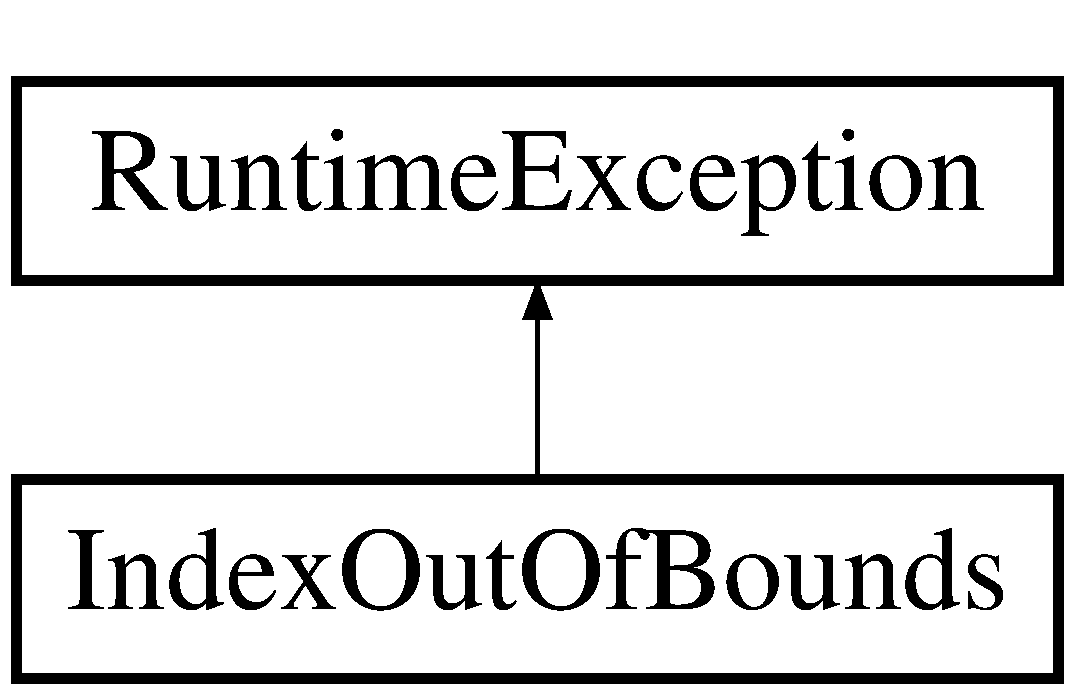
\includegraphics[height=2.000000cm]{class_runtime_exception}
\end{center}
\end{figure}
\subsection*{Public Member Functions}
\begin{DoxyCompactItemize}
\item 
\hyperlink{class_runtime_exception_ae86e31b0c6d823e7097be268d502140e}{Runtime\+Exception} ()
\begin{DoxyCompactList}\small\item\em Create a default \hyperlink{class_runtime_exception}{Runtime\+Exception}. \end{DoxyCompactList}\item 
\hyperlink{class_runtime_exception_aa088818f62804acab75a1a1c6b6c504c}{Runtime\+Exception} (const std\+::string \&err)
\begin{DoxyCompactList}\small\item\em Create a \hyperlink{class_runtime_exception}{Runtime\+Exception} with a custom error message. \end{DoxyCompactList}\item 
std\+::string \hyperlink{class_runtime_exception_abc78ad4db28b4a879725f4c6b7622405}{get\+Message} () const 
\begin{DoxyCompactList}\small\item\em Return the error message to the client. \end{DoxyCompactList}\end{DoxyCompactItemize}
\subsection*{Protected Attributes}
\begin{DoxyCompactItemize}
\item 
std\+::string \hyperlink{class_runtime_exception_a02a4bcba40c9cf48be9565556940eef9}{error\+Msg}
\begin{DoxyCompactList}\small\item\em The error message. \end{DoxyCompactList}\end{DoxyCompactItemize}


\subsection{Detailed Description}
A generic runtime exception class. \begin{DoxyAuthor}{Author}
Jesse Mazzella 
\end{DoxyAuthor}


Definition at line 17 of file Exceptions.\+h.



\subsection{Constructor \& Destructor Documentation}
\index{Runtime\+Exception@{Runtime\+Exception}!Runtime\+Exception@{Runtime\+Exception}}
\index{Runtime\+Exception@{Runtime\+Exception}!Runtime\+Exception@{Runtime\+Exception}}
\subsubsection[{\texorpdfstring{Runtime\+Exception()}{RuntimeException()}}]{\setlength{\rightskip}{0pt plus 5cm}Runtime\+Exception\+::\+Runtime\+Exception (
\begin{DoxyParamCaption}
{}
\end{DoxyParamCaption}
)\hspace{0.3cm}{\ttfamily [inline]}}\hypertarget{class_runtime_exception_ae86e31b0c6d823e7097be268d502140e}{}\label{class_runtime_exception_ae86e31b0c6d823e7097be268d502140e}


Create a default \hyperlink{class_runtime_exception}{Runtime\+Exception}. 



Definition at line 21 of file Exceptions.\+h.

\index{Runtime\+Exception@{Runtime\+Exception}!Runtime\+Exception@{Runtime\+Exception}}
\index{Runtime\+Exception@{Runtime\+Exception}!Runtime\+Exception@{Runtime\+Exception}}
\subsubsection[{\texorpdfstring{Runtime\+Exception(const std\+::string \&err)}{RuntimeException(const std::string &err)}}]{\setlength{\rightskip}{0pt plus 5cm}Runtime\+Exception\+::\+Runtime\+Exception (
\begin{DoxyParamCaption}
\item[{const std\+::string \&}]{err}
\end{DoxyParamCaption}
)\hspace{0.3cm}{\ttfamily [inline]}}\hypertarget{class_runtime_exception_aa088818f62804acab75a1a1c6b6c504c}{}\label{class_runtime_exception_aa088818f62804acab75a1a1c6b6c504c}


Create a \hyperlink{class_runtime_exception}{Runtime\+Exception} with a custom error message. 



Definition at line 25 of file Exceptions.\+h.



\subsection{Member Function Documentation}
\index{Runtime\+Exception@{Runtime\+Exception}!get\+Message@{get\+Message}}
\index{get\+Message@{get\+Message}!Runtime\+Exception@{Runtime\+Exception}}
\subsubsection[{\texorpdfstring{get\+Message() const }{getMessage() const }}]{\setlength{\rightskip}{0pt plus 5cm}std\+::string Runtime\+Exception\+::get\+Message (
\begin{DoxyParamCaption}
{}
\end{DoxyParamCaption}
) const\hspace{0.3cm}{\ttfamily [inline]}}\hypertarget{class_runtime_exception_abc78ad4db28b4a879725f4c6b7622405}{}\label{class_runtime_exception_abc78ad4db28b4a879725f4c6b7622405}


Return the error message to the client. 

\begin{DoxyAuthor}{Author}
Jesse Mazzella 
\end{DoxyAuthor}
\begin{DoxyReturn}{Returns}
The related error message as a string 
\end{DoxyReturn}


Definition at line 33 of file Exceptions.\+h.



\subsection{Member Data Documentation}
\index{Runtime\+Exception@{Runtime\+Exception}!error\+Msg@{error\+Msg}}
\index{error\+Msg@{error\+Msg}!Runtime\+Exception@{Runtime\+Exception}}
\subsubsection[{\texorpdfstring{error\+Msg}{errorMsg}}]{\setlength{\rightskip}{0pt plus 5cm}std\+::string Runtime\+Exception\+::error\+Msg\hspace{0.3cm}{\ttfamily [protected]}}\hypertarget{class_runtime_exception_a02a4bcba40c9cf48be9565556940eef9}{}\label{class_runtime_exception_a02a4bcba40c9cf48be9565556940eef9}


The error message. 



Definition at line 37 of file Exceptions.\+h.



The documentation for this class was generated from the following file\+:\begin{DoxyCompactItemize}
\item 
src/header/\hyperlink{_exceptions_8h}{Exceptions.\+h}\end{DoxyCompactItemize}

\hypertarget{class_souvenir_table_model}{}\section{Souvenir\+Table\+Model Class Reference}
\label{class_souvenir_table_model}\index{Souvenir\+Table\+Model@{Souvenir\+Table\+Model}}


{\ttfamily \#include $<$souvenirtablemodel.\+h$>$}

Inheritance diagram for Souvenir\+Table\+Model\+:\begin{figure}[H]
\begin{center}
\leavevmode
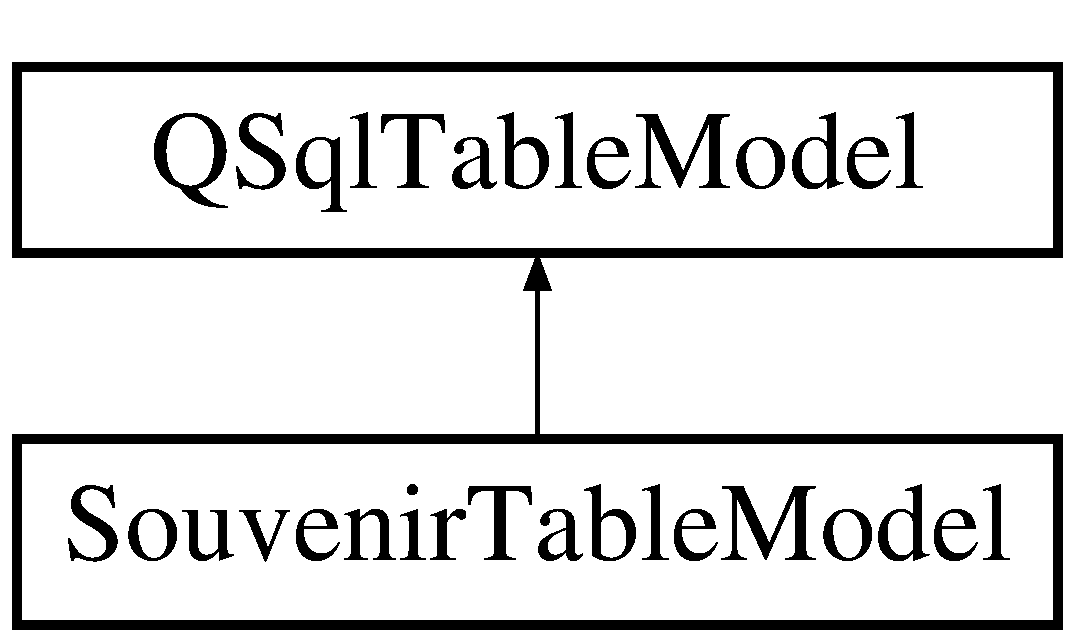
\includegraphics[height=2.000000cm]{class_souvenir_table_model}
\end{center}
\end{figure}
\subsection*{Public Types}
\begin{DoxyCompactItemize}
\item 
enum \hyperlink{class_souvenir_table_model_a678ba75189e65ec4902d8d33873c1467}{Fields} \{ \hyperlink{class_souvenir_table_model_a678ba75189e65ec4902d8d33873c1467a7e415b557e37cfaaebfe6f7f4dcad957}{S\+T\+A\+D\+I\+U\+M\+\_\+\+ID}, 
\hyperlink{class_souvenir_table_model_a678ba75189e65ec4902d8d33873c1467a1562f7948671504ce66f4abc2e781b91}{N\+A\+ME}, 
\hyperlink{class_souvenir_table_model_a678ba75189e65ec4902d8d33873c1467a2b832d332664f9bf0211f8254557e1b2}{P\+R\+I\+CE}
 \}
\end{DoxyCompactItemize}
\subsection*{Public Member Functions}
\begin{DoxyCompactItemize}
\item 
\hyperlink{class_souvenir_table_model_a61ddb206432239d2f3c0c0081e529903}{Souvenir\+Table\+Model} (Q\+Object $\ast$parent, \hyperlink{class_database}{Database} $\ast$db)
\item 
\hyperlink{class_souvenir_table_model_aa77b7b9de97a059a7a0b608ec18599fc}{Souvenir\+Table\+Model} (Q\+Object $\ast$parent, \hyperlink{class_database}{Database} $\ast$db, int stadium\+Id)
\item 
void \hyperlink{class_souvenir_table_model_a8a7188e334bdb2f11a20f598f305a5c9}{Initialize} (int stadium\+Id=-\/1)
\end{DoxyCompactItemize}


\subsection{Detailed Description}


Definition at line 8 of file souvenirtablemodel.\+h.



\subsection{Member Enumeration Documentation}
\index{Souvenir\+Table\+Model@{Souvenir\+Table\+Model}!Fields@{Fields}}
\index{Fields@{Fields}!Souvenir\+Table\+Model@{Souvenir\+Table\+Model}}
\subsubsection[{\texorpdfstring{Fields}{Fields}}]{\setlength{\rightskip}{0pt plus 5cm}enum {\bf Souvenir\+Table\+Model\+::\+Fields}}\hypertarget{class_souvenir_table_model_a678ba75189e65ec4902d8d33873c1467}{}\label{class_souvenir_table_model_a678ba75189e65ec4902d8d33873c1467}
\begin{Desc}
\item[Enumerator]\par
\begin{description}
\index{S\+T\+A\+D\+I\+U\+M\+\_\+\+ID@{S\+T\+A\+D\+I\+U\+M\+\_\+\+ID}!Souvenir\+Table\+Model@{Souvenir\+Table\+Model}}\index{Souvenir\+Table\+Model@{Souvenir\+Table\+Model}!S\+T\+A\+D\+I\+U\+M\+\_\+\+ID@{S\+T\+A\+D\+I\+U\+M\+\_\+\+ID}}\item[{\em 
S\+T\+A\+D\+I\+U\+M\+\_\+\+ID\hypertarget{class_souvenir_table_model_a678ba75189e65ec4902d8d33873c1467a7e415b557e37cfaaebfe6f7f4dcad957}{}\label{class_souvenir_table_model_a678ba75189e65ec4902d8d33873c1467a7e415b557e37cfaaebfe6f7f4dcad957}
}]\index{N\+A\+ME@{N\+A\+ME}!Souvenir\+Table\+Model@{Souvenir\+Table\+Model}}\index{Souvenir\+Table\+Model@{Souvenir\+Table\+Model}!N\+A\+ME@{N\+A\+ME}}\item[{\em 
N\+A\+ME\hypertarget{class_souvenir_table_model_a678ba75189e65ec4902d8d33873c1467a1562f7948671504ce66f4abc2e781b91}{}\label{class_souvenir_table_model_a678ba75189e65ec4902d8d33873c1467a1562f7948671504ce66f4abc2e781b91}
}]\index{P\+R\+I\+CE@{P\+R\+I\+CE}!Souvenir\+Table\+Model@{Souvenir\+Table\+Model}}\index{Souvenir\+Table\+Model@{Souvenir\+Table\+Model}!P\+R\+I\+CE@{P\+R\+I\+CE}}\item[{\em 
P\+R\+I\+CE\hypertarget{class_souvenir_table_model_a678ba75189e65ec4902d8d33873c1467a2b832d332664f9bf0211f8254557e1b2}{}\label{class_souvenir_table_model_a678ba75189e65ec4902d8d33873c1467a2b832d332664f9bf0211f8254557e1b2}
}]\end{description}
\end{Desc}


Definition at line 13 of file souvenirtablemodel.\+h.



\subsection{Constructor \& Destructor Documentation}
\index{Souvenir\+Table\+Model@{Souvenir\+Table\+Model}!Souvenir\+Table\+Model@{Souvenir\+Table\+Model}}
\index{Souvenir\+Table\+Model@{Souvenir\+Table\+Model}!Souvenir\+Table\+Model@{Souvenir\+Table\+Model}}
\subsubsection[{\texorpdfstring{Souvenir\+Table\+Model(\+Q\+Object $\ast$parent, Database $\ast$db)}{SouvenirTableModel(QObject *parent, Database *db)}}]{\setlength{\rightskip}{0pt plus 5cm}Souvenir\+Table\+Model\+::\+Souvenir\+Table\+Model (
\begin{DoxyParamCaption}
\item[{Q\+Object $\ast$}]{parent, }
\item[{{\bf Database} $\ast$}]{db}
\end{DoxyParamCaption}
)}\hypertarget{class_souvenir_table_model_a61ddb206432239d2f3c0c0081e529903}{}\label{class_souvenir_table_model_a61ddb206432239d2f3c0c0081e529903}


Definition at line 3 of file souvenirtablemodel.\+cpp.

\index{Souvenir\+Table\+Model@{Souvenir\+Table\+Model}!Souvenir\+Table\+Model@{Souvenir\+Table\+Model}}
\index{Souvenir\+Table\+Model@{Souvenir\+Table\+Model}!Souvenir\+Table\+Model@{Souvenir\+Table\+Model}}
\subsubsection[{\texorpdfstring{Souvenir\+Table\+Model(\+Q\+Object $\ast$parent, Database $\ast$db, int stadium\+Id)}{SouvenirTableModel(QObject *parent, Database *db, int stadiumId)}}]{\setlength{\rightskip}{0pt plus 5cm}Souvenir\+Table\+Model\+::\+Souvenir\+Table\+Model (
\begin{DoxyParamCaption}
\item[{Q\+Object $\ast$}]{parent, }
\item[{{\bf Database} $\ast$}]{db, }
\item[{int}]{stadium\+Id}
\end{DoxyParamCaption}
)}\hypertarget{class_souvenir_table_model_aa77b7b9de97a059a7a0b608ec18599fc}{}\label{class_souvenir_table_model_aa77b7b9de97a059a7a0b608ec18599fc}


Definition at line 8 of file souvenirtablemodel.\+cpp.



\subsection{Member Function Documentation}
\index{Souvenir\+Table\+Model@{Souvenir\+Table\+Model}!Initialize@{Initialize}}
\index{Initialize@{Initialize}!Souvenir\+Table\+Model@{Souvenir\+Table\+Model}}
\subsubsection[{\texorpdfstring{Initialize(int stadium\+Id=-\/1)}{Initialize(int stadiumId=-1)}}]{\setlength{\rightskip}{0pt plus 5cm}void Souvenir\+Table\+Model\+::\+Initialize (
\begin{DoxyParamCaption}
\item[{int}]{stadium\+Id = {\ttfamily -\/1}}
\end{DoxyParamCaption}
)}\hypertarget{class_souvenir_table_model_a8a7188e334bdb2f11a20f598f305a5c9}{}\label{class_souvenir_table_model_a8a7188e334bdb2f11a20f598f305a5c9}


Definition at line 13 of file souvenirtablemodel.\+cpp.



The documentation for this class was generated from the following files\+:\begin{DoxyCompactItemize}
\item 
src/header/\hyperlink{souvenirtablemodel_8h}{souvenirtablemodel.\+h}\item 
src/source/\hyperlink{souvenirtablemodel_8cpp}{souvenirtablemodel.\+cpp}\end{DoxyCompactItemize}

\hypertarget{class_stadium_details}{}\section{Stadium\+Details Class Reference}
\label{class_stadium_details}\index{Stadium\+Details@{Stadium\+Details}}


{\ttfamily \#include $<$stadiumdetails.\+h$>$}

Inheritance diagram for Stadium\+Details\+:\begin{figure}[H]
\begin{center}
\leavevmode
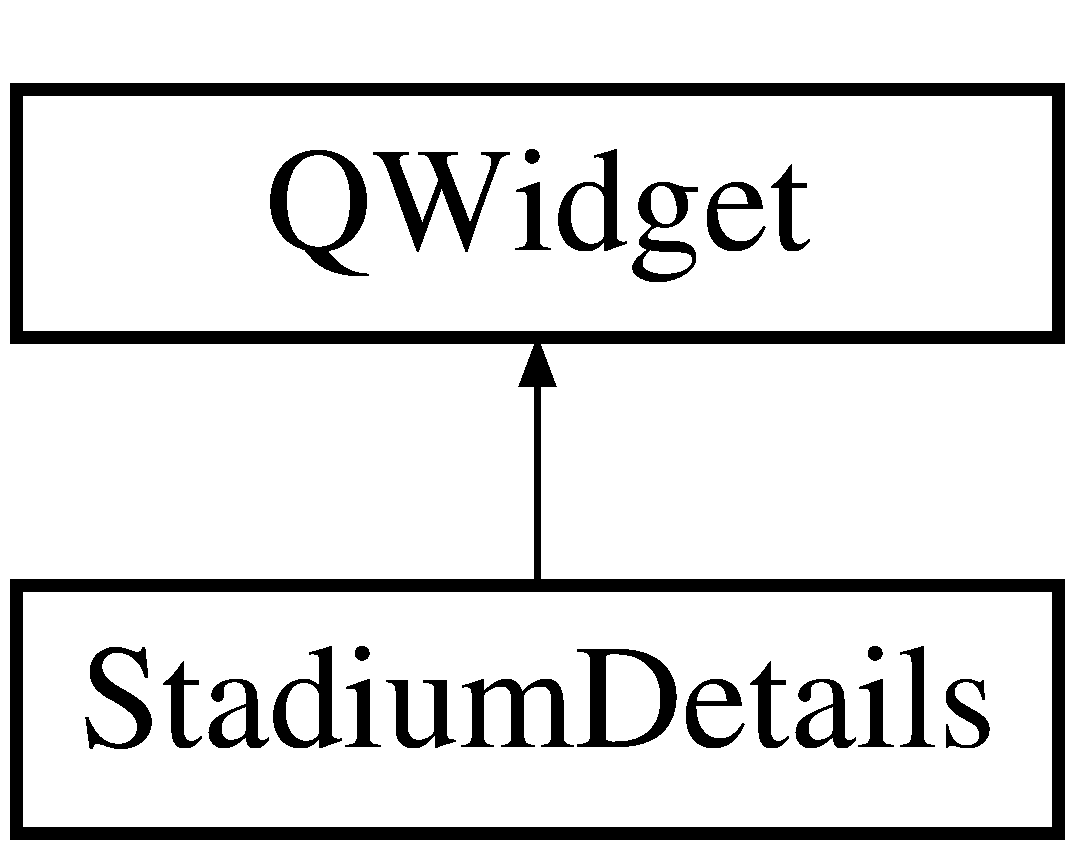
\includegraphics[height=2.000000cm]{class_stadium_details}
\end{center}
\end{figure}
\subsection*{Public Slots}
\begin{DoxyCompactItemize}
\item 
void \hyperlink{class_stadium_details_a0868c6ed136cf59f3ab4afe71d01833c}{refresh\+Models} ()
\item 
void \hyperlink{class_stadium_details_a011c0e49c863d55f34de7bfd85a9fdf3}{toggle\+Admin\+Functions} (bool is\+Admin)
\begin{DoxyCompactList}\small\item\em \hyperlink{class_stadium_details_a011c0e49c863d55f34de7bfd85a9fdf3}{Stadium\+Details\+::toggle\+Admin\+Functions} Hide/unhide and enable/disable all buttons and features for admin use only. \end{DoxyCompactList}\item 
void \hyperlink{class_stadium_details_a9e249b86f719d2f23aa1eb55de90a287}{initialize\+Stadium\+Table} (\hyperlink{class_stadium_table_model}{Stadium\+Table\+Model} $\ast$stadium\+Model)
\begin{DoxyCompactList}\small\item\em \hyperlink{class_stadium_details_a9e249b86f719d2f23aa1eb55de90a287}{Stadium\+Details\+::initialize\+Stadium\+Table}. \end{DoxyCompactList}\item 
void \hyperlink{class_stadium_details_a5f3a91287d68868421f77dd1d275b307}{initialize\+Souvenir\+Table} (\hyperlink{class_souvenir_table_model}{Souvenir\+Table\+Model} $\ast$souvenir\+Model)
\begin{DoxyCompactList}\small\item\em \hyperlink{class_stadium_details_a5f3a91287d68868421f77dd1d275b307}{Stadium\+Details\+::initialize\+Souvenir\+Table} Initializes the souvenir\+Table using the model emitted from main\+Window. \end{DoxyCompactList}\item 
void \hyperlink{class_stadium_details_afae941fb61d0b6845cd3200d5003297a}{update\+Total\+Revenue} ()
\end{DoxyCompactItemize}
\subsection*{Public Member Functions}
\begin{DoxyCompactItemize}
\item 
\hyperlink{class_stadium_details_a8879d228339f65e4685c03db50ae2856}{Stadium\+Details} (Q\+Widget $\ast$parent=0, \hyperlink{class_database}{Database} $\ast$db=0)
\item 
void \hyperlink{class_stadium_details_ad0399417bccb9ee2109ec5b5857b844c}{initialize\+Stadium\+View} ()
\begin{DoxyCompactList}\small\item\em \hyperlink{class_stadium_details_ad0399417bccb9ee2109ec5b5857b844c}{Stadium\+Details\+::initialize\+Stadium\+View} Initialize settings for stadium table view. \end{DoxyCompactList}\item 
void \hyperlink{class_stadium_details_ac5634fbdb4be32116854f7ddf55cb845}{initialize\+Souvenir\+View} ()
\begin{DoxyCompactList}\small\item\em \hyperlink{class_stadium_details_ac5634fbdb4be32116854f7ddf55cb845}{Stadium\+Details\+::initialize\+Souvenir\+View} Initialize settings for souvenir table view. \end{DoxyCompactList}\item 
\hyperlink{class_stadium_details_a8ace510be03c29948b2ced20ac056865}{$\sim$\+Stadium\+Details} ()
\end{DoxyCompactItemize}


\subsection{Detailed Description}


Definition at line 15 of file stadiumdetails.\+h.



\subsection{Constructor \& Destructor Documentation}
\index{Stadium\+Details@{Stadium\+Details}!Stadium\+Details@{Stadium\+Details}}
\index{Stadium\+Details@{Stadium\+Details}!Stadium\+Details@{Stadium\+Details}}
\subsubsection[{\texorpdfstring{Stadium\+Details(\+Q\+Widget $\ast$parent=0, Database $\ast$db=0)}{StadiumDetails(QWidget *parent=0, Database *db=0)}}]{\setlength{\rightskip}{0pt plus 5cm}Stadium\+Details\+::\+Stadium\+Details (
\begin{DoxyParamCaption}
\item[{Q\+Widget $\ast$}]{parent = {\ttfamily 0}, }
\item[{{\bf Database} $\ast$}]{db = {\ttfamily 0}}
\end{DoxyParamCaption}
)\hspace{0.3cm}{\ttfamily [explicit]}}\hypertarget{class_stadium_details_a8879d228339f65e4685c03db50ae2856}{}\label{class_stadium_details_a8879d228339f65e4685c03db50ae2856}


Definition at line 4 of file stadiumdetails.\+cpp.

\index{Stadium\+Details@{Stadium\+Details}!````~Stadium\+Details@{$\sim$\+Stadium\+Details}}
\index{````~Stadium\+Details@{$\sim$\+Stadium\+Details}!Stadium\+Details@{Stadium\+Details}}
\subsubsection[{\texorpdfstring{$\sim$\+Stadium\+Details()}{~StadiumDetails()}}]{\setlength{\rightskip}{0pt plus 5cm}Stadium\+Details\+::$\sim$\+Stadium\+Details (
\begin{DoxyParamCaption}
{}
\end{DoxyParamCaption}
)}\hypertarget{class_stadium_details_a8ace510be03c29948b2ced20ac056865}{}\label{class_stadium_details_a8ace510be03c29948b2ced20ac056865}


Definition at line 88 of file stadiumdetails.\+cpp.



\subsection{Member Function Documentation}
\index{Stadium\+Details@{Stadium\+Details}!initialize\+Souvenir\+Table@{initialize\+Souvenir\+Table}}
\index{initialize\+Souvenir\+Table@{initialize\+Souvenir\+Table}!Stadium\+Details@{Stadium\+Details}}
\subsubsection[{\texorpdfstring{initialize\+Souvenir\+Table}{initializeSouvenirTable}}]{\setlength{\rightskip}{0pt plus 5cm}void Stadium\+Details\+::initialize\+Souvenir\+Table (
\begin{DoxyParamCaption}
\item[{{\bf Souvenir\+Table\+Model} $\ast$}]{souvenir\+Model}
\end{DoxyParamCaption}
)\hspace{0.3cm}{\ttfamily [slot]}}\hypertarget{class_stadium_details_a5f3a91287d68868421f77dd1d275b307}{}\label{class_stadium_details_a5f3a91287d68868421f77dd1d275b307}


\hyperlink{class_stadium_details_a5f3a91287d68868421f77dd1d275b307}{Stadium\+Details\+::initialize\+Souvenir\+Table} Initializes the souvenir\+Table using the model emitted from main\+Window. 


\begin{DoxyParams}{Parameters}
{\em souvenir\+Model} & The model emitted from main\+Window \\
\hline
\end{DoxyParams}


Definition at line 157 of file stadiumdetails.\+cpp.

\index{Stadium\+Details@{Stadium\+Details}!initialize\+Souvenir\+View@{initialize\+Souvenir\+View}}
\index{initialize\+Souvenir\+View@{initialize\+Souvenir\+View}!Stadium\+Details@{Stadium\+Details}}
\subsubsection[{\texorpdfstring{initialize\+Souvenir\+View()}{initializeSouvenirView()}}]{\setlength{\rightskip}{0pt plus 5cm}void Stadium\+Details\+::initialize\+Souvenir\+View (
\begin{DoxyParamCaption}
{}
\end{DoxyParamCaption}
)}\hypertarget{class_stadium_details_ac5634fbdb4be32116854f7ddf55cb845}{}\label{class_stadium_details_ac5634fbdb4be32116854f7ddf55cb845}


\hyperlink{class_stadium_details_ac5634fbdb4be32116854f7ddf55cb845}{Stadium\+Details\+::initialize\+Souvenir\+View} Initialize settings for souvenir table view. 



Definition at line 55 of file stadiumdetails.\+cpp.

\index{Stadium\+Details@{Stadium\+Details}!initialize\+Stadium\+Table@{initialize\+Stadium\+Table}}
\index{initialize\+Stadium\+Table@{initialize\+Stadium\+Table}!Stadium\+Details@{Stadium\+Details}}
\subsubsection[{\texorpdfstring{initialize\+Stadium\+Table}{initializeStadiumTable}}]{\setlength{\rightskip}{0pt plus 5cm}void Stadium\+Details\+::initialize\+Stadium\+Table (
\begin{DoxyParamCaption}
\item[{{\bf Stadium\+Table\+Model} $\ast$}]{stadium\+Model}
\end{DoxyParamCaption}
)\hspace{0.3cm}{\ttfamily [slot]}}\hypertarget{class_stadium_details_a9e249b86f719d2f23aa1eb55de90a287}{}\label{class_stadium_details_a9e249b86f719d2f23aa1eb55de90a287}


\hyperlink{class_stadium_details_a9e249b86f719d2f23aa1eb55de90a287}{Stadium\+Details\+::initialize\+Stadium\+Table}. 


\begin{DoxyParams}{Parameters}
{\em stadium\+Model} & The model to initialize the table to. \\
\hline
\end{DoxyParams}


Definition at line 139 of file stadiumdetails.\+cpp.

\index{Stadium\+Details@{Stadium\+Details}!initialize\+Stadium\+View@{initialize\+Stadium\+View}}
\index{initialize\+Stadium\+View@{initialize\+Stadium\+View}!Stadium\+Details@{Stadium\+Details}}
\subsubsection[{\texorpdfstring{initialize\+Stadium\+View()}{initializeStadiumView()}}]{\setlength{\rightskip}{0pt plus 5cm}void Stadium\+Details\+::initialize\+Stadium\+View (
\begin{DoxyParamCaption}
{}
\end{DoxyParamCaption}
)}\hypertarget{class_stadium_details_ad0399417bccb9ee2109ec5b5857b844c}{}\label{class_stadium_details_ad0399417bccb9ee2109ec5b5857b844c}


\hyperlink{class_stadium_details_ad0399417bccb9ee2109ec5b5857b844c}{Stadium\+Details\+::initialize\+Stadium\+View} Initialize settings for stadium table view. 



Definition at line 18 of file stadiumdetails.\+cpp.

\index{Stadium\+Details@{Stadium\+Details}!refresh\+Models@{refresh\+Models}}
\index{refresh\+Models@{refresh\+Models}!Stadium\+Details@{Stadium\+Details}}
\subsubsection[{\texorpdfstring{refresh\+Models}{refreshModels}}]{\setlength{\rightskip}{0pt plus 5cm}void Stadium\+Details\+::refresh\+Models (
\begin{DoxyParamCaption}
{}
\end{DoxyParamCaption}
)\hspace{0.3cm}{\ttfamily [slot]}}\hypertarget{class_stadium_details_a0868c6ed136cf59f3ab4afe71d01833c}{}\label{class_stadium_details_a0868c6ed136cf59f3ab4afe71d01833c}


Definition at line 93 of file stadiumdetails.\+cpp.

\index{Stadium\+Details@{Stadium\+Details}!toggle\+Admin\+Functions@{toggle\+Admin\+Functions}}
\index{toggle\+Admin\+Functions@{toggle\+Admin\+Functions}!Stadium\+Details@{Stadium\+Details}}
\subsubsection[{\texorpdfstring{toggle\+Admin\+Functions}{toggleAdminFunctions}}]{\setlength{\rightskip}{0pt plus 5cm}void Stadium\+Details\+::toggle\+Admin\+Functions (
\begin{DoxyParamCaption}
\item[{bool}]{is\+Admin}
\end{DoxyParamCaption}
)\hspace{0.3cm}{\ttfamily [slot]}}\hypertarget{class_stadium_details_a011c0e49c863d55f34de7bfd85a9fdf3}{}\label{class_stadium_details_a011c0e49c863d55f34de7bfd85a9fdf3}


\hyperlink{class_stadium_details_a011c0e49c863d55f34de7bfd85a9fdf3}{Stadium\+Details\+::toggle\+Admin\+Functions} Hide/unhide and enable/disable all buttons and features for admin use only. 


\begin{DoxyParams}{Parameters}
{\em is\+Admin} & true if user is admin \\
\hline
\end{DoxyParams}


Definition at line 105 of file stadiumdetails.\+cpp.

\index{Stadium\+Details@{Stadium\+Details}!update\+Total\+Revenue@{update\+Total\+Revenue}}
\index{update\+Total\+Revenue@{update\+Total\+Revenue}!Stadium\+Details@{Stadium\+Details}}
\subsubsection[{\texorpdfstring{update\+Total\+Revenue}{updateTotalRevenue}}]{\setlength{\rightskip}{0pt plus 5cm}void Stadium\+Details\+::update\+Total\+Revenue (
\begin{DoxyParamCaption}
{}
\end{DoxyParamCaption}
)\hspace{0.3cm}{\ttfamily [slot]}}\hypertarget{class_stadium_details_afae941fb61d0b6845cd3200d5003297a}{}\label{class_stadium_details_afae941fb61d0b6845cd3200d5003297a}


Definition at line 170 of file stadiumdetails.\+cpp.



The documentation for this class was generated from the following files\+:\begin{DoxyCompactItemize}
\item 
src/header/\hyperlink{stadiumdetails_8h}{stadiumdetails.\+h}\item 
src/source/\hyperlink{stadiumdetails_8cpp}{stadiumdetails.\+cpp}\end{DoxyCompactItemize}

\hypertarget{class_stadium_table_model}{}\section{Stadium\+Table\+Model Class Reference}
\label{class_stadium_table_model}\index{Stadium\+Table\+Model@{Stadium\+Table\+Model}}


{\ttfamily \#include $<$stadiumtablemodel.\+h$>$}

Inheritance diagram for Stadium\+Table\+Model\+:\begin{figure}[H]
\begin{center}
\leavevmode
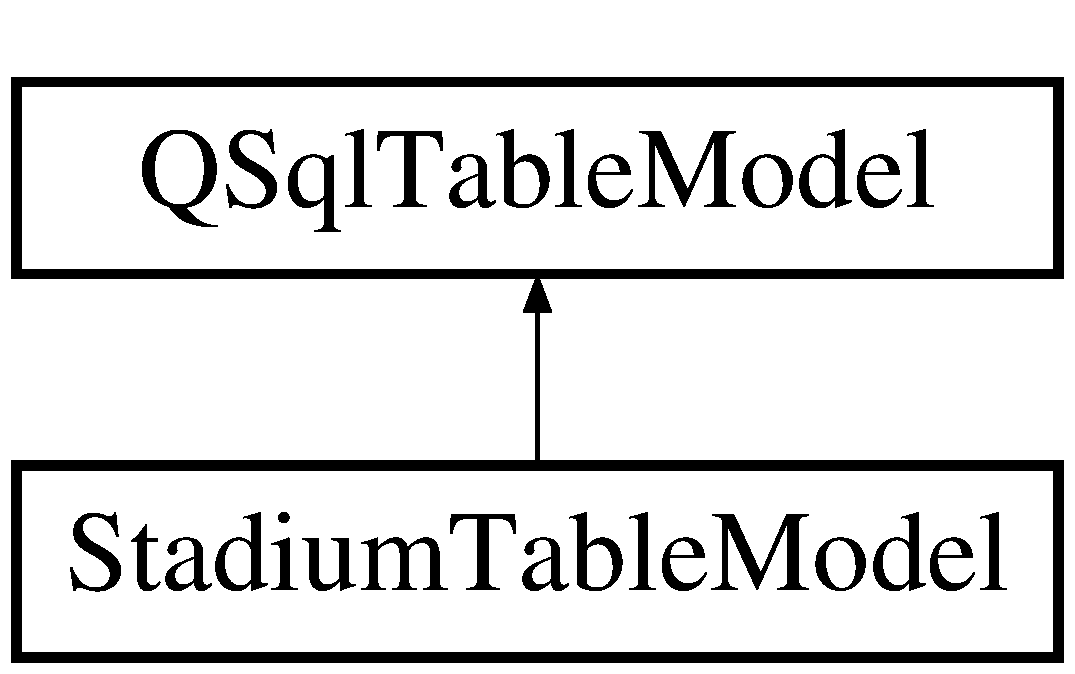
\includegraphics[height=2.000000cm]{class_stadium_table_model}
\end{center}
\end{figure}
\subsection*{Public Types}
\begin{DoxyCompactItemize}
\item 
enum \hyperlink{class_stadium_table_model_a424b16a0e2e9f5a5a75c022e7d4024c6}{Fields} \{ \\*
\hyperlink{class_stadium_table_model_a424b16a0e2e9f5a5a75c022e7d4024c6a4d04365bdaed0d9317978fc7c96a793c}{ID}, 
\hyperlink{class_stadium_table_model_a424b16a0e2e9f5a5a75c022e7d4024c6a4c0deadbbab13afa73f88a06d4d558da}{N\+A\+ME}, 
\hyperlink{class_stadium_table_model_a424b16a0e2e9f5a5a75c022e7d4024c6aabc647ecc94e3742c100f962928613c9}{T\+E\+AM}, 
\hyperlink{class_stadium_table_model_a424b16a0e2e9f5a5a75c022e7d4024c6a75659731ead2f2f1e142cfd188ccd914}{A\+D\+D\+R\+E\+SS}, 
\\*
\hyperlink{class_stadium_table_model_a424b16a0e2e9f5a5a75c022e7d4024c6adfdcc68b010e3b52cffaea6193f1f0fb}{P\+H\+O\+NE}, 
\hyperlink{class_stadium_table_model_a424b16a0e2e9f5a5a75c022e7d4024c6aa4bde58dc1989a25742a85e47a206129}{D\+A\+TE}, 
\hyperlink{class_stadium_table_model_a424b16a0e2e9f5a5a75c022e7d4024c6a7a4ab0f9fabfccd9ddaf68d2317f512d}{C\+A\+P\+A\+C\+I\+TY}, 
\hyperlink{class_stadium_table_model_a424b16a0e2e9f5a5a75c022e7d4024c6adf90b7a6c4a9d287c9ef1f8c2a2c38f0}{T\+U\+RF}, 
\\*
\hyperlink{class_stadium_table_model_a424b16a0e2e9f5a5a75c022e7d4024c6a06ec4a04eb9cf1d5cbef36e5f478909d}{R\+E\+V\+E\+N\+UE}, 
\hyperlink{class_stadium_table_model_a424b16a0e2e9f5a5a75c022e7d4024c6a379beec0cf9f661b52a9d268de70c4ca}{L\+E\+A\+G\+UE}
 \}
\end{DoxyCompactItemize}
\subsection*{Public Member Functions}
\begin{DoxyCompactItemize}
\item 
\hyperlink{class_stadium_table_model_afef158fb1fee5aab9902048db5a69bf2}{Stadium\+Table\+Model} (Q\+Object $\ast$parent, \hyperlink{class_database}{Database} $\ast$db)
\begin{DoxyCompactList}\small\item\em \hyperlink{class_stadium_table_model_afef158fb1fee5aab9902048db5a69bf2}{Stadium\+Table\+Model\+::\+Stadium\+Table\+Model} A reusable model class for displaying the list of stadiums in a table\+View. \end{DoxyCompactList}\item 
void \hyperlink{class_stadium_table_model_acf30d2a9c04b9691bbe15056c0804423}{Initialize} ()
\begin{DoxyCompactList}\small\item\em \hyperlink{class_stadium_table_model_acf30d2a9c04b9691bbe15056c0804423}{Stadium\+Table\+Model\+::\+Initialize} Initialize all of the settings for the stadium table model. This includes selecting which S\+QL table to display, setting header values, and setting the table as uneditable unless manually submitted. \end{DoxyCompactList}\end{DoxyCompactItemize}


\subsection{Detailed Description}


Definition at line 7 of file stadiumtablemodel.\+h.



\subsection{Member Enumeration Documentation}
\index{Stadium\+Table\+Model@{Stadium\+Table\+Model}!Fields@{Fields}}
\index{Fields@{Fields}!Stadium\+Table\+Model@{Stadium\+Table\+Model}}
\subsubsection[{\texorpdfstring{Fields}{Fields}}]{\setlength{\rightskip}{0pt plus 5cm}enum {\bf Stadium\+Table\+Model\+::\+Fields}}\hypertarget{class_stadium_table_model_a424b16a0e2e9f5a5a75c022e7d4024c6}{}\label{class_stadium_table_model_a424b16a0e2e9f5a5a75c022e7d4024c6}
\begin{Desc}
\item[Enumerator]\par
\begin{description}
\index{ID@{ID}!Stadium\+Table\+Model@{Stadium\+Table\+Model}}\index{Stadium\+Table\+Model@{Stadium\+Table\+Model}!ID@{ID}}\item[{\em 
ID\hypertarget{class_stadium_table_model_a424b16a0e2e9f5a5a75c022e7d4024c6a4d04365bdaed0d9317978fc7c96a793c}{}\label{class_stadium_table_model_a424b16a0e2e9f5a5a75c022e7d4024c6a4d04365bdaed0d9317978fc7c96a793c}
}]\index{N\+A\+ME@{N\+A\+ME}!Stadium\+Table\+Model@{Stadium\+Table\+Model}}\index{Stadium\+Table\+Model@{Stadium\+Table\+Model}!N\+A\+ME@{N\+A\+ME}}\item[{\em 
N\+A\+ME\hypertarget{class_stadium_table_model_a424b16a0e2e9f5a5a75c022e7d4024c6a4c0deadbbab13afa73f88a06d4d558da}{}\label{class_stadium_table_model_a424b16a0e2e9f5a5a75c022e7d4024c6a4c0deadbbab13afa73f88a06d4d558da}
}]\index{T\+E\+AM@{T\+E\+AM}!Stadium\+Table\+Model@{Stadium\+Table\+Model}}\index{Stadium\+Table\+Model@{Stadium\+Table\+Model}!T\+E\+AM@{T\+E\+AM}}\item[{\em 
T\+E\+AM\hypertarget{class_stadium_table_model_a424b16a0e2e9f5a5a75c022e7d4024c6aabc647ecc94e3742c100f962928613c9}{}\label{class_stadium_table_model_a424b16a0e2e9f5a5a75c022e7d4024c6aabc647ecc94e3742c100f962928613c9}
}]\index{A\+D\+D\+R\+E\+SS@{A\+D\+D\+R\+E\+SS}!Stadium\+Table\+Model@{Stadium\+Table\+Model}}\index{Stadium\+Table\+Model@{Stadium\+Table\+Model}!A\+D\+D\+R\+E\+SS@{A\+D\+D\+R\+E\+SS}}\item[{\em 
A\+D\+D\+R\+E\+SS\hypertarget{class_stadium_table_model_a424b16a0e2e9f5a5a75c022e7d4024c6a75659731ead2f2f1e142cfd188ccd914}{}\label{class_stadium_table_model_a424b16a0e2e9f5a5a75c022e7d4024c6a75659731ead2f2f1e142cfd188ccd914}
}]\index{P\+H\+O\+NE@{P\+H\+O\+NE}!Stadium\+Table\+Model@{Stadium\+Table\+Model}}\index{Stadium\+Table\+Model@{Stadium\+Table\+Model}!P\+H\+O\+NE@{P\+H\+O\+NE}}\item[{\em 
P\+H\+O\+NE\hypertarget{class_stadium_table_model_a424b16a0e2e9f5a5a75c022e7d4024c6adfdcc68b010e3b52cffaea6193f1f0fb}{}\label{class_stadium_table_model_a424b16a0e2e9f5a5a75c022e7d4024c6adfdcc68b010e3b52cffaea6193f1f0fb}
}]\index{D\+A\+TE@{D\+A\+TE}!Stadium\+Table\+Model@{Stadium\+Table\+Model}}\index{Stadium\+Table\+Model@{Stadium\+Table\+Model}!D\+A\+TE@{D\+A\+TE}}\item[{\em 
D\+A\+TE\hypertarget{class_stadium_table_model_a424b16a0e2e9f5a5a75c022e7d4024c6aa4bde58dc1989a25742a85e47a206129}{}\label{class_stadium_table_model_a424b16a0e2e9f5a5a75c022e7d4024c6aa4bde58dc1989a25742a85e47a206129}
}]\index{C\+A\+P\+A\+C\+I\+TY@{C\+A\+P\+A\+C\+I\+TY}!Stadium\+Table\+Model@{Stadium\+Table\+Model}}\index{Stadium\+Table\+Model@{Stadium\+Table\+Model}!C\+A\+P\+A\+C\+I\+TY@{C\+A\+P\+A\+C\+I\+TY}}\item[{\em 
C\+A\+P\+A\+C\+I\+TY\hypertarget{class_stadium_table_model_a424b16a0e2e9f5a5a75c022e7d4024c6a7a4ab0f9fabfccd9ddaf68d2317f512d}{}\label{class_stadium_table_model_a424b16a0e2e9f5a5a75c022e7d4024c6a7a4ab0f9fabfccd9ddaf68d2317f512d}
}]\index{T\+U\+RF@{T\+U\+RF}!Stadium\+Table\+Model@{Stadium\+Table\+Model}}\index{Stadium\+Table\+Model@{Stadium\+Table\+Model}!T\+U\+RF@{T\+U\+RF}}\item[{\em 
T\+U\+RF\hypertarget{class_stadium_table_model_a424b16a0e2e9f5a5a75c022e7d4024c6adf90b7a6c4a9d287c9ef1f8c2a2c38f0}{}\label{class_stadium_table_model_a424b16a0e2e9f5a5a75c022e7d4024c6adf90b7a6c4a9d287c9ef1f8c2a2c38f0}
}]\index{R\+E\+V\+E\+N\+UE@{R\+E\+V\+E\+N\+UE}!Stadium\+Table\+Model@{Stadium\+Table\+Model}}\index{Stadium\+Table\+Model@{Stadium\+Table\+Model}!R\+E\+V\+E\+N\+UE@{R\+E\+V\+E\+N\+UE}}\item[{\em 
R\+E\+V\+E\+N\+UE\hypertarget{class_stadium_table_model_a424b16a0e2e9f5a5a75c022e7d4024c6a06ec4a04eb9cf1d5cbef36e5f478909d}{}\label{class_stadium_table_model_a424b16a0e2e9f5a5a75c022e7d4024c6a06ec4a04eb9cf1d5cbef36e5f478909d}
}]\index{L\+E\+A\+G\+UE@{L\+E\+A\+G\+UE}!Stadium\+Table\+Model@{Stadium\+Table\+Model}}\index{Stadium\+Table\+Model@{Stadium\+Table\+Model}!L\+E\+A\+G\+UE@{L\+E\+A\+G\+UE}}\item[{\em 
L\+E\+A\+G\+UE\hypertarget{class_stadium_table_model_a424b16a0e2e9f5a5a75c022e7d4024c6a379beec0cf9f661b52a9d268de70c4ca}{}\label{class_stadium_table_model_a424b16a0e2e9f5a5a75c022e7d4024c6a379beec0cf9f661b52a9d268de70c4ca}
}]\end{description}
\end{Desc}


Definition at line 13 of file stadiumtablemodel.\+h.



\subsection{Constructor \& Destructor Documentation}
\index{Stadium\+Table\+Model@{Stadium\+Table\+Model}!Stadium\+Table\+Model@{Stadium\+Table\+Model}}
\index{Stadium\+Table\+Model@{Stadium\+Table\+Model}!Stadium\+Table\+Model@{Stadium\+Table\+Model}}
\subsubsection[{\texorpdfstring{Stadium\+Table\+Model(\+Q\+Object $\ast$parent, Database $\ast$db)}{StadiumTableModel(QObject *parent, Database *db)}}]{\setlength{\rightskip}{0pt plus 5cm}Stadium\+Table\+Model\+::\+Stadium\+Table\+Model (
\begin{DoxyParamCaption}
\item[{Q\+Object $\ast$}]{parent, }
\item[{{\bf Database} $\ast$}]{db}
\end{DoxyParamCaption}
)}\hypertarget{class_stadium_table_model_afef158fb1fee5aab9902048db5a69bf2}{}\label{class_stadium_table_model_afef158fb1fee5aab9902048db5a69bf2}


\hyperlink{class_stadium_table_model_afef158fb1fee5aab9902048db5a69bf2}{Stadium\+Table\+Model\+::\+Stadium\+Table\+Model} A reusable model class for displaying the list of stadiums in a table\+View. 


\begin{DoxyParams}{Parameters}
{\em parent} & The parent object \\
\hline
{\em db} & The database to read from \\
\hline
\end{DoxyParams}


Definition at line 9 of file stadiumtablemodel.\+cpp.



\subsection{Member Function Documentation}
\index{Stadium\+Table\+Model@{Stadium\+Table\+Model}!Initialize@{Initialize}}
\index{Initialize@{Initialize}!Stadium\+Table\+Model@{Stadium\+Table\+Model}}
\subsubsection[{\texorpdfstring{Initialize()}{Initialize()}}]{\setlength{\rightskip}{0pt plus 5cm}void Stadium\+Table\+Model\+::\+Initialize (
\begin{DoxyParamCaption}
{}
\end{DoxyParamCaption}
)}\hypertarget{class_stadium_table_model_acf30d2a9c04b9691bbe15056c0804423}{}\label{class_stadium_table_model_acf30d2a9c04b9691bbe15056c0804423}


\hyperlink{class_stadium_table_model_acf30d2a9c04b9691bbe15056c0804423}{Stadium\+Table\+Model\+::\+Initialize} Initialize all of the settings for the stadium table model. This includes selecting which S\+QL table to display, setting header values, and setting the table as uneditable unless manually submitted. 



Definition at line 20 of file stadiumtablemodel.\+cpp.



The documentation for this class was generated from the following files\+:\begin{DoxyCompactItemize}
\item 
src/header/\hyperlink{stadiumtablemodel_8h}{stadiumtablemodel.\+h}\item 
src/source/\hyperlink{stadiumtablemodel_8cpp}{stadiumtablemodel.\+cpp}\end{DoxyCompactItemize}

\hypertarget{class_test___main}{}\section{Test\+\_\+\+Main Class Reference}
\label{class_test___main}\index{Test\+\_\+\+Main@{Test\+\_\+\+Main}}
Inheritance diagram for Test\+\_\+\+Main\+:\begin{figure}[H]
\begin{center}
\leavevmode
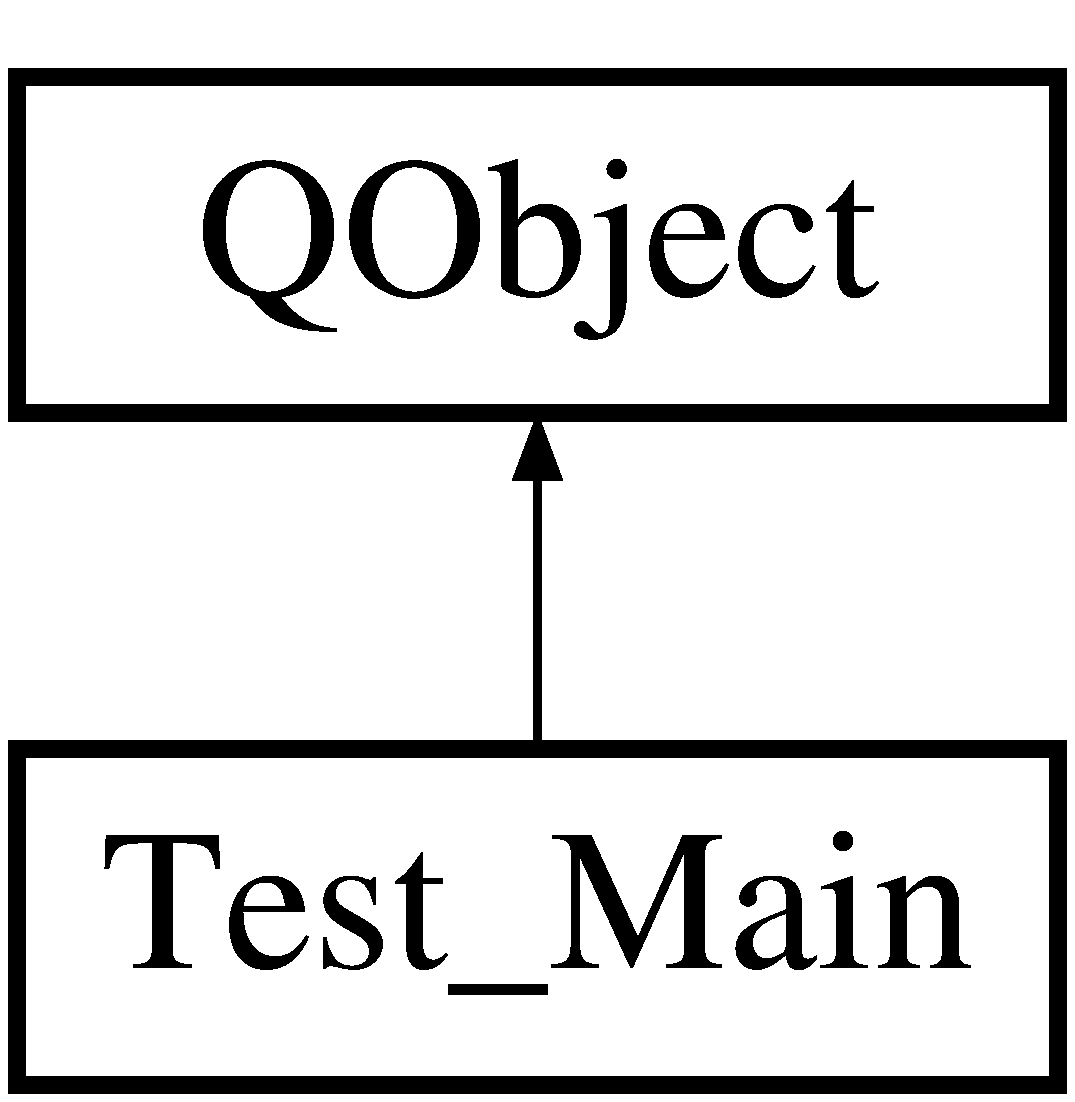
\includegraphics[height=2.000000cm]{class_test___main}
\end{center}
\end{figure}


\subsection{Detailed Description}


Definition at line 6 of file test\+\_\+main.\+cpp.



The documentation for this class was generated from the following file\+:\begin{DoxyCompactItemize}
\item 
test/\hyperlink{test__main_8cpp}{test\+\_\+main.\+cpp}\end{DoxyCompactItemize}

\hypertarget{class_trip_summary}{}\section{Trip\+Summary Class Reference}
\label{class_trip_summary}\index{Trip\+Summary@{Trip\+Summary}}


{\ttfamily \#include $<$tripsummary.\+h$>$}

Inheritance diagram for Trip\+Summary\+:\begin{figure}[H]
\begin{center}
\leavevmode
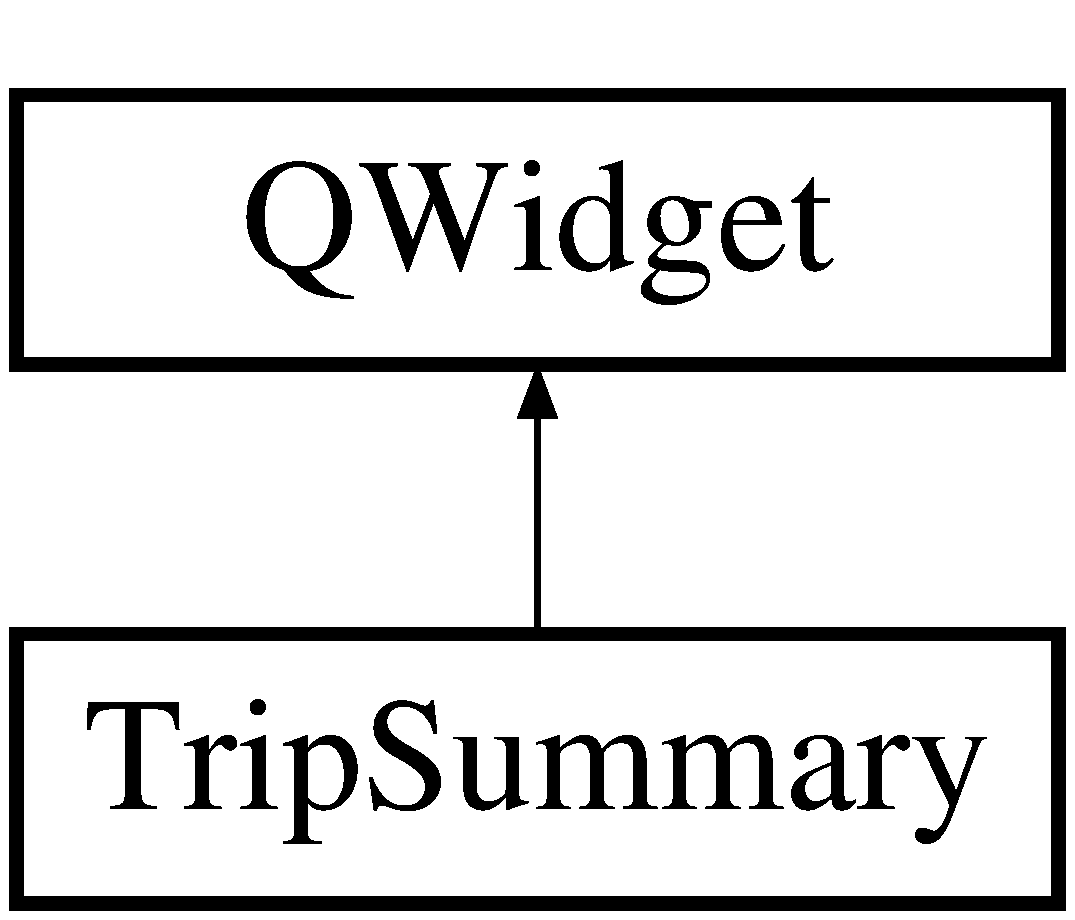
\includegraphics[height=2.000000cm]{class_trip_summary}
\end{center}
\end{figure}
\subsection*{Signals}
\begin{DoxyCompactItemize}
\item 
void \hyperlink{class_trip_summary_a42d4d98e730c27b257b61e878169a687}{finish\+Trip} (bool)
\begin{DoxyCompactList}\small\item\em Send a signal when the user presses the finish button. \end{DoxyCompactList}\end{DoxyCompactItemize}
\subsection*{Public Member Functions}
\begin{DoxyCompactItemize}
\item 
\hyperlink{class_trip_summary_aa8bae5ef064b751299de19a622403431}{Trip\+Summary} (Q\+Widget $\ast$parent=0, \hyperlink{class_database}{Database} $\ast$db=0)
\item 
\hyperlink{class_trip_summary_a6e3c73fb47c7068fe216dd8d0d913586}{$\sim$\+Trip\+Summary} ()
\item 
void \hyperlink{class_trip_summary_ab6f01bddea6c40bd95698fa53e091f18}{populate\+Trip\+Path} (\hyperlink{class_q_list}{Q\+List}$<$ \hyperlink{class_vertex}{Vertex} $>$ path\+Of\+Trip, bool is\+Custom\+Trip=true)
\begin{DoxyCompactList}\small\item\em populate\+Trip\+Path Takes in a \hyperlink{class_q_list}{Q\+List} of $<$\+Vertex$>$ to be displayed on the list, assumes the list is ordered in the sortest path \end{DoxyCompactList}\item 
void \hyperlink{class_trip_summary_a09328d4f72b93d3b33a43d3bb16c1c0d}{populate\+Purchase\+Reciept} (\hyperlink{class_q_list}{Q\+List}$<$ \hyperlink{struct_purchase_window_1_1purchase_info}{Purchase\+Window\+::purchase\+Info} $>$ purchases)
\begin{DoxyCompactList}\small\item\em populate\+Purchase\+Reciept This method will take in the purchase table and display the users total spent When the item is hovered over, it will tell you the total revenue of the stadium that sovenir came from \end{DoxyCompactList}\item 
void \hyperlink{class_trip_summary_afd9cdb3b7cd6f096b896c1d474d3ed54}{clear\+Data} ()
\begin{DoxyCompactList}\small\item\em clear\+Data Clears the data on the list so that it can be reused for next time \end{DoxyCompactList}\end{DoxyCompactItemize}


\subsection{Detailed Description}


Definition at line 12 of file tripsummary.\+h.



\subsection{Constructor \& Destructor Documentation}
\index{Trip\+Summary@{Trip\+Summary}!Trip\+Summary@{Trip\+Summary}}
\index{Trip\+Summary@{Trip\+Summary}!Trip\+Summary@{Trip\+Summary}}
\subsubsection[{\texorpdfstring{Trip\+Summary(\+Q\+Widget $\ast$parent=0, Database $\ast$db=0)}{TripSummary(QWidget *parent=0, Database *db=0)}}]{\setlength{\rightskip}{0pt plus 5cm}Trip\+Summary\+::\+Trip\+Summary (
\begin{DoxyParamCaption}
\item[{Q\+Widget $\ast$}]{parent = {\ttfamily 0}, }
\item[{{\bf Database} $\ast$}]{db = {\ttfamily 0}}
\end{DoxyParamCaption}
)\hspace{0.3cm}{\ttfamily [explicit]}}\hypertarget{class_trip_summary_aa8bae5ef064b751299de19a622403431}{}\label{class_trip_summary_aa8bae5ef064b751299de19a622403431}


Definition at line 4 of file tripsummary.\+cpp.

\index{Trip\+Summary@{Trip\+Summary}!````~Trip\+Summary@{$\sim$\+Trip\+Summary}}
\index{````~Trip\+Summary@{$\sim$\+Trip\+Summary}!Trip\+Summary@{Trip\+Summary}}
\subsubsection[{\texorpdfstring{$\sim$\+Trip\+Summary()}{~TripSummary()}}]{\setlength{\rightskip}{0pt plus 5cm}Trip\+Summary\+::$\sim$\+Trip\+Summary (
\begin{DoxyParamCaption}
{}
\end{DoxyParamCaption}
)}\hypertarget{class_trip_summary_a6e3c73fb47c7068fe216dd8d0d913586}{}\label{class_trip_summary_a6e3c73fb47c7068fe216dd8d0d913586}


Definition at line 15 of file tripsummary.\+cpp.



\subsection{Member Function Documentation}
\index{Trip\+Summary@{Trip\+Summary}!clear\+Data@{clear\+Data}}
\index{clear\+Data@{clear\+Data}!Trip\+Summary@{Trip\+Summary}}
\subsubsection[{\texorpdfstring{clear\+Data()}{clearData()}}]{\setlength{\rightskip}{0pt plus 5cm}void Trip\+Summary\+::clear\+Data (
\begin{DoxyParamCaption}
{}
\end{DoxyParamCaption}
)}\hypertarget{class_trip_summary_afd9cdb3b7cd6f096b896c1d474d3ed54}{}\label{class_trip_summary_afd9cdb3b7cd6f096b896c1d474d3ed54}


clear\+Data Clears the data on the list so that it can be reused for next time 

\hyperlink{class_trip_summary_afd9cdb3b7cd6f096b896c1d474d3ed54}{Trip\+Summary\+::clear\+Data} Clears the two lists. 

Definition at line 193 of file tripsummary.\+cpp.

\index{Trip\+Summary@{Trip\+Summary}!finish\+Trip@{finish\+Trip}}
\index{finish\+Trip@{finish\+Trip}!Trip\+Summary@{Trip\+Summary}}
\subsubsection[{\texorpdfstring{finish\+Trip}{finishTrip}}]{\setlength{\rightskip}{0pt plus 5cm}void Trip\+Summary\+::finish\+Trip (
\begin{DoxyParamCaption}
\item[{bool}]{}
\end{DoxyParamCaption}
)\hspace{0.3cm}{\ttfamily [signal]}}\hypertarget{class_trip_summary_a42d4d98e730c27b257b61e878169a687}{}\label{class_trip_summary_a42d4d98e730c27b257b61e878169a687}


Send a signal when the user presses the finish button. 

\index{Trip\+Summary@{Trip\+Summary}!populate\+Purchase\+Reciept@{populate\+Purchase\+Reciept}}
\index{populate\+Purchase\+Reciept@{populate\+Purchase\+Reciept}!Trip\+Summary@{Trip\+Summary}}
\subsubsection[{\texorpdfstring{populate\+Purchase\+Reciept(\+Q\+List$<$ Purchase\+Window\+::purchase\+Info $>$ purchases)}{populatePurchaseReciept(QList< PurchaseWindow::purchaseInfo > purchases)}}]{\setlength{\rightskip}{0pt plus 5cm}void Trip\+Summary\+::populate\+Purchase\+Reciept (
\begin{DoxyParamCaption}
\item[{{\bf Q\+List}$<$ {\bf Purchase\+Window\+::purchase\+Info} $>$}]{purchases}
\end{DoxyParamCaption}
)}\hypertarget{class_trip_summary_a09328d4f72b93d3b33a43d3bb16c1c0d}{}\label{class_trip_summary_a09328d4f72b93d3b33a43d3bb16c1c0d}


populate\+Purchase\+Reciept This method will take in the purchase table and display the users total spent When the item is hovered over, it will tell you the total revenue of the stadium that sovenir came from 

\hyperlink{class_trip_summary_a09328d4f72b93d3b33a43d3bb16c1c0d}{Trip\+Summary\+::populate\+Purchase\+Reciept} Populates the List widget with the information of purchases.


\begin{DoxyParams}{Parameters}
{\em purchases} & -\/ \hyperlink{class_q_list}{Q\+List} of Structure purchase\+Info\\
\hline
{\em purchases} & \\
\hline
\end{DoxyParams}


Definition at line 129 of file tripsummary.\+cpp.

\index{Trip\+Summary@{Trip\+Summary}!populate\+Trip\+Path@{populate\+Trip\+Path}}
\index{populate\+Trip\+Path@{populate\+Trip\+Path}!Trip\+Summary@{Trip\+Summary}}
\subsubsection[{\texorpdfstring{populate\+Trip\+Path(\+Q\+List$<$ Vertex $>$ path\+Of\+Trip, bool is\+Custom\+Trip=true)}{populateTripPath(QList< Vertex > pathOfTrip, bool isCustomTrip=true)}}]{\setlength{\rightskip}{0pt plus 5cm}void Trip\+Summary\+::populate\+Trip\+Path (
\begin{DoxyParamCaption}
\item[{{\bf Q\+List}$<$ {\bf Vertex} $>$}]{path\+Of\+Trip, }
\item[{bool}]{is\+Custom\+Trip = {\ttfamily true}}
\end{DoxyParamCaption}
)}\hypertarget{class_trip_summary_ab6f01bddea6c40bd95698fa53e091f18}{}\label{class_trip_summary_ab6f01bddea6c40bd95698fa53e091f18}


populate\+Trip\+Path Takes in a \hyperlink{class_q_list}{Q\+List} of $<$\+Vertex$>$ to be displayed on the list, assumes the list is ordered in the sortest path 

\hyperlink{class_trip_summary_ab6f01bddea6c40bd95698fa53e091f18}{Trip\+Summary\+::populate\+Trip\+Path} Method will populate the trip path list with given data from the algorithm.


\begin{DoxyParams}{Parameters}
{\em path\+Of\+Trip} & \\
\hline
\end{DoxyParams}


Definition at line 24 of file tripsummary.\+cpp.



The documentation for this class was generated from the following files\+:\begin{DoxyCompactItemize}
\item 
src/header/\hyperlink{tripsummary_8h}{tripsummary.\+h}\item 
src/source/\hyperlink{tripsummary_8cpp}{tripsummary.\+cpp}\end{DoxyCompactItemize}

\hypertarget{class_vertex}{}\section{Vertex Class Reference}
\label{class_vertex}\index{Vertex@{Vertex}}


{\ttfamily \#include $<$vertex.\+h$>$}

\subsection*{Public Member Functions}
\begin{DoxyCompactItemize}
\item 
\hyperlink{class_vertex_a97488994a2482d70da74e1b91d40e169}{Vertex} ()
\begin{DoxyCompactList}\small\item\em \hyperlink{class_vertex}{Vertex} Default \hyperlink{class_vertex}{Vertex} constructor. \end{DoxyCompactList}\item 
\hyperlink{class_vertex_ade66bd39dce6ed6f1bdf4d93af045f56}{Vertex} (int id, Q\+String name, int distance)
\begin{DoxyCompactList}\small\item\em \hyperlink{class_vertex}{Vertex} Non-\/default \hyperlink{class_vertex}{Vertex} Constructor. Takes in the ID and name of the vertex as it is being instatiated. \end{DoxyCompactList}\item 
int \hyperlink{class_vertex_aa61ee83bfe1b0c80f0b554663bdbd2da}{get\+Id} () const 
\begin{DoxyCompactList}\small\item\em get\+Id \end{DoxyCompactList}\item 
Q\+String \hyperlink{class_vertex_af870d1f4fd501f7167c71461e3764cf5}{get\+Name} () const 
\begin{DoxyCompactList}\small\item\em get\+Name \end{DoxyCompactList}\item 
int \hyperlink{class_vertex_a754900c038f5a3b1da20c0448eb97fce}{get\+Distance} () const 
\begin{DoxyCompactList}\small\item\em get\+Distance This distance is not the distance representing a single vertex but the distance between this vertex and another a \textquotesingle{}source\textquotesingle{} vertex during a single shortest path search \end{DoxyCompactList}\item 
void \hyperlink{class_vertex_a0b766cc3ce251348af422c0773bb4359}{set\+Id} (int id)
\begin{DoxyCompactList}\small\item\em set\+Id Set the ID of the vertex \end{DoxyCompactList}\item 
void \hyperlink{class_vertex_a19650c9cd9e30c07897b70781bee3e31}{set\+Name} (Q\+String name)
\begin{DoxyCompactList}\small\item\em set\+Name Set the name of the vertex \end{DoxyCompactList}\item 
void \hyperlink{class_vertex_aeecd5db632f599376c1bfa3737348434}{set\+Parent} (int p)
\begin{DoxyCompactList}\small\item\em set\+Parent Set the parent of the current vertex to p \end{DoxyCompactList}\item 
void \hyperlink{class_vertex_a020868955e2e501f13bd4f5b6d1d5a23}{set\+Distance} (int d)
\begin{DoxyCompactList}\small\item\em set\+Distance Set the distance of the vertex traveled between 2 vertices \end{DoxyCompactList}\item 
bool \hyperlink{class_vertex_a7f1217525ed5dffeeebc7201d4827e7c}{operator==} (const \hyperlink{class_vertex}{Vertex} \&v) const 
\begin{DoxyCompactList}\small\item\em operator == Overloaded comparison operator. Compares the distance, ID and the name over the 2 vertices. Returns true if they are equal, false otherwise. \end{DoxyCompactList}\item 
bool \hyperlink{class_vertex_ae704d41fe2ff1316201b85c5ec2d7d5b}{operator!=} (const \hyperlink{class_vertex}{Vertex} \&v) const 
\begin{DoxyCompactList}\small\item\em operator != Overloaded comparison operator to see if the two vertices are not the same vertex. Compares the ID and the name of the vertex as its determining factors of equality. \end{DoxyCompactList}\item 
bool \hyperlink{class_vertex_a82b7bdf14f62f4a0e13dce7f33f9713d}{operator$<$} (const \hyperlink{class_vertex}{Vertex} \&v) const 
\begin{DoxyCompactList}\small\item\em operator $<$ Overloaded less than operator to compare this vertex distance and the given vertex v \end{DoxyCompactList}\item 
bool \hyperlink{class_vertex_a85bf76a3a2212f0d5d81e327f9eecd65}{operator$>$} (const \hyperlink{class_vertex}{Vertex} \&v) const 
\begin{DoxyCompactList}\small\item\em operator $>$ Overloaded greater than operator to compare this vertex distance and the given vertex v \end{DoxyCompactList}\item 
bool \hyperlink{class_vertex_a9a9c7ae24773341a58343809e5fa511f}{operator$>$=} (const \hyperlink{class_vertex}{Vertex} \&v) const 
\begin{DoxyCompactList}\small\item\em operator $>$= Overloaded greater than or equal operator to compare this vertex distance and the given vertex v \end{DoxyCompactList}\item 
bool \hyperlink{class_vertex_a5c45e745c39aeea6dd713d3ce7b5c023}{operator$<$=} (const \hyperlink{class_vertex}{Vertex} \&v) const 
\begin{DoxyCompactList}\small\item\em operator $<$= Overloaded less than or equal operator to compare this vertex distance and the given vertex v \end{DoxyCompactList}\item 
\hyperlink{class_vertex}{Vertex} $\ast$ \hyperlink{class_vertex_ae08494c23f6d03a242c2ff0ef0679865}{operator=} (const \hyperlink{class_vertex}{Vertex} \&v)
\begin{DoxyCompactList}\small\item\em operator = Overloaded assignment operator to assign the values of the given vertex v to this vertex. Assigns the distance, id and name this vertex then returns \textquotesingle{}this\textquotesingle{} to the calling object. \end{DoxyCompactList}\item 
void \hyperlink{class_vertex_a700e64ce39492162ebd5ec2cb5cdea45}{add\+Edge} (\hyperlink{struct_edge}{Edge} edge)
\begin{DoxyCompactList}\small\item\em add\+Edge Takes the given edge and insert it into an internal adjacency list. \end{DoxyCompactList}\item 
\hyperlink{struct_edge}{Edge} \hyperlink{class_vertex_a32d9da19ba0b88642691f743092a6bea}{get\+Nearest\+Edge} ()
\begin{DoxyCompactList}\small\item\em get\+Nearest\+Edge Method will grab the edge with the least amount of weight (distance) the current vertex. It removes the edge for the min-\/heap stored in the vertex and appends it to a list of edges that has been removed. \end{DoxyCompactList}\item 
int \hyperlink{class_vertex_a0988796727c76d1161c656f696ee0997}{get\+Num\+Edges} () const 
\begin{DoxyCompactList}\small\item\em get\+Num\+Edges This method will return the number of adjacent edges that exsists between this vertex and other vertices. \end{DoxyCompactList}\item 
bool \hyperlink{class_vertex_ab6f75fe6517f8a56d7b033510e71a9ea}{has\+Edges} () const 
\begin{DoxyCompactList}\small\item\em has\+Edges Returns a boolean value if the current vertex has adjacent edges left in it\textquotesingle{}s priority queue adjacency list. \end{DoxyCompactList}\item 
int \hyperlink{class_vertex_a57eba4a06c19525ba9753058061c370c}{get\+Parent} () const 
\begin{DoxyCompactList}\small\item\em get\+Parent Method returns the ID integer value of the it\textquotesingle{}s parent vertex. This is only established after a path has been taken using Dijkstra\textquotesingle{}s algorithm or calculating the minimum spanning tree. \end{DoxyCompactList}\item 
void \hyperlink{class_vertex_a81f32ef92752b1b4832e026b03e0dd2b}{reinitialize\+Edges} ()
\begin{DoxyCompactList}\small\item\em reinitialize\+Edges This method iterates the vertex\textquotesingle{}s current edges and places them back into it\textquotesingle{}s own priority queue (adjacency list). \end{DoxyCompactList}\item 
\hyperlink{struct_edge}{Edge} \hyperlink{class_vertex_a4fd094f20a327502d4c5752354ed0bf1}{get\+Next\+Edge} ()
\begin{DoxyCompactList}\small\item\em get\+Next\+Edge this will return the next edge available in verticee adjacency list. \end{DoxyCompactList}\item 
void \hyperlink{class_vertex_a34cfbcd18c862c2532be2ecfd790c428}{set\+Queue\+Position} (int pos)
\begin{DoxyCompactList}\small\item\em set\+Queue\+Position Sets the vertex index that is relative to its position in the stored object that it is located in, such as a map, queue or a vector. \end{DoxyCompactList}\item 
int \hyperlink{class_vertex_aae3e291772ef43309d3609800aa4c1c3}{get\+Queue\+Position} () const 
\begin{DoxyCompactList}\small\item\em get\+Queue\+Position This returns the vertices index of the position / location that it is located in a container object. \end{DoxyCompactList}\end{DoxyCompactItemize}


\subsection{Detailed Description}


Definition at line 28 of file vertex.\+h.



\subsection{Constructor \& Destructor Documentation}
\index{Vertex@{Vertex}!Vertex@{Vertex}}
\index{Vertex@{Vertex}!Vertex@{Vertex}}
\subsubsection[{\texorpdfstring{Vertex()}{Vertex()}}]{\setlength{\rightskip}{0pt plus 5cm}Vertex\+::\+Vertex (
\begin{DoxyParamCaption}
{}
\end{DoxyParamCaption}
)\hspace{0.3cm}{\ttfamily [inline]}}\hypertarget{class_vertex_a97488994a2482d70da74e1b91d40e169}{}\label{class_vertex_a97488994a2482d70da74e1b91d40e169}


\hyperlink{class_vertex}{Vertex} Default \hyperlink{class_vertex}{Vertex} constructor. 



Definition at line 35 of file vertex.\+h.

\index{Vertex@{Vertex}!Vertex@{Vertex}}
\index{Vertex@{Vertex}!Vertex@{Vertex}}
\subsubsection[{\texorpdfstring{Vertex(int id, Q\+String name, int distance)}{Vertex(int id, QString name, int distance)}}]{\setlength{\rightskip}{0pt plus 5cm}Vertex\+::\+Vertex (
\begin{DoxyParamCaption}
\item[{int}]{id, }
\item[{Q\+String}]{name, }
\item[{int}]{distance}
\end{DoxyParamCaption}
)\hspace{0.3cm}{\ttfamily [inline]}}\hypertarget{class_vertex_ade66bd39dce6ed6f1bdf4d93af045f56}{}\label{class_vertex_ade66bd39dce6ed6f1bdf4d93af045f56}


\hyperlink{class_vertex}{Vertex} Non-\/default \hyperlink{class_vertex}{Vertex} Constructor. Takes in the ID and name of the vertex as it is being instatiated. 


\begin{DoxyParams}{Parameters}
{\em id} & \\
\hline
{\em name} & \\
\hline
\end{DoxyParams}


Definition at line 50 of file vertex.\+h.



\subsection{Member Function Documentation}
\index{Vertex@{Vertex}!add\+Edge@{add\+Edge}}
\index{add\+Edge@{add\+Edge}!Vertex@{Vertex}}
\subsubsection[{\texorpdfstring{add\+Edge(\+Edge edge)}{addEdge(Edge edge)}}]{\setlength{\rightskip}{0pt plus 5cm}void Vertex\+::add\+Edge (
\begin{DoxyParamCaption}
\item[{{\bf Edge}}]{edge}
\end{DoxyParamCaption}
)\hspace{0.3cm}{\ttfamily [inline]}}\hypertarget{class_vertex_a700e64ce39492162ebd5ec2cb5cdea45}{}\label{class_vertex_a700e64ce39492162ebd5ec2cb5cdea45}


add\+Edge Takes the given edge and insert it into an internal adjacency list. 


\begin{DoxyParams}{Parameters}
{\em edge} & \\
\hline
\end{DoxyParams}


Definition at line 226 of file vertex.\+h.

\index{Vertex@{Vertex}!get\+Distance@{get\+Distance}}
\index{get\+Distance@{get\+Distance}!Vertex@{Vertex}}
\subsubsection[{\texorpdfstring{get\+Distance() const }{getDistance() const }}]{\setlength{\rightskip}{0pt plus 5cm}int Vertex\+::get\+Distance (
\begin{DoxyParamCaption}
{}
\end{DoxyParamCaption}
) const\hspace{0.3cm}{\ttfamily [inline]}}\hypertarget{class_vertex_a754900c038f5a3b1da20c0448eb97fce}{}\label{class_vertex_a754900c038f5a3b1da20c0448eb97fce}


get\+Distance This distance is not the distance representing a single vertex but the distance between this vertex and another a \textquotesingle{}source\textquotesingle{} vertex during a single shortest path search 

\begin{DoxyReturn}{Returns}
the distance stored in the vertex 
\end{DoxyReturn}


Definition at line 86 of file vertex.\+h.

\index{Vertex@{Vertex}!get\+Id@{get\+Id}}
\index{get\+Id@{get\+Id}!Vertex@{Vertex}}
\subsubsection[{\texorpdfstring{get\+Id() const }{getId() const }}]{\setlength{\rightskip}{0pt plus 5cm}int Vertex\+::get\+Id (
\begin{DoxyParamCaption}
{}
\end{DoxyParamCaption}
) const\hspace{0.3cm}{\ttfamily [inline]}}\hypertarget{class_vertex_aa61ee83bfe1b0c80f0b554663bdbd2da}{}\label{class_vertex_aa61ee83bfe1b0c80f0b554663bdbd2da}


get\+Id 

\begin{DoxyReturn}{Returns}
The id of the vertex 
\end{DoxyReturn}


Definition at line 65 of file vertex.\+h.

\index{Vertex@{Vertex}!get\+Name@{get\+Name}}
\index{get\+Name@{get\+Name}!Vertex@{Vertex}}
\subsubsection[{\texorpdfstring{get\+Name() const }{getName() const }}]{\setlength{\rightskip}{0pt plus 5cm}Q\+String Vertex\+::get\+Name (
\begin{DoxyParamCaption}
{}
\end{DoxyParamCaption}
) const\hspace{0.3cm}{\ttfamily [inline]}}\hypertarget{class_vertex_af870d1f4fd501f7167c71461e3764cf5}{}\label{class_vertex_af870d1f4fd501f7167c71461e3764cf5}


get\+Name 

\begin{DoxyReturn}{Returns}
The name of the vertex 
\end{DoxyReturn}


Definition at line 74 of file vertex.\+h.

\index{Vertex@{Vertex}!get\+Nearest\+Edge@{get\+Nearest\+Edge}}
\index{get\+Nearest\+Edge@{get\+Nearest\+Edge}!Vertex@{Vertex}}
\subsubsection[{\texorpdfstring{get\+Nearest\+Edge()}{getNearestEdge()}}]{\setlength{\rightskip}{0pt plus 5cm}{\bf Edge} Vertex\+::get\+Nearest\+Edge (
\begin{DoxyParamCaption}
{}
\end{DoxyParamCaption}
)\hspace{0.3cm}{\ttfamily [inline]}}\hypertarget{class_vertex_a32d9da19ba0b88642691f743092a6bea}{}\label{class_vertex_a32d9da19ba0b88642691f743092a6bea}


get\+Nearest\+Edge Method will grab the edge with the least amount of weight (distance) the current vertex. It removes the edge for the min-\/heap stored in the vertex and appends it to a list of edges that has been removed. 

\begin{DoxyReturn}{Returns}

\end{DoxyReturn}


Definition at line 239 of file vertex.\+h.

\index{Vertex@{Vertex}!get\+Next\+Edge@{get\+Next\+Edge}}
\index{get\+Next\+Edge@{get\+Next\+Edge}!Vertex@{Vertex}}
\subsubsection[{\texorpdfstring{get\+Next\+Edge()}{getNextEdge()}}]{\setlength{\rightskip}{0pt plus 5cm}{\bf Edge} Vertex\+::get\+Next\+Edge (
\begin{DoxyParamCaption}
{}
\end{DoxyParamCaption}
)\hspace{0.3cm}{\ttfamily [inline]}}\hypertarget{class_vertex_a4fd094f20a327502d4c5752354ed0bf1}{}\label{class_vertex_a4fd094f20a327502d4c5752354ed0bf1}


get\+Next\+Edge this will return the next edge available in verticee adjacency list. 

\begin{DoxyReturn}{Returns}
edge object of the adj list 
\end{DoxyReturn}


Definition at line 310 of file vertex.\+h.

\index{Vertex@{Vertex}!get\+Num\+Edges@{get\+Num\+Edges}}
\index{get\+Num\+Edges@{get\+Num\+Edges}!Vertex@{Vertex}}
\subsubsection[{\texorpdfstring{get\+Num\+Edges() const }{getNumEdges() const }}]{\setlength{\rightskip}{0pt plus 5cm}int Vertex\+::get\+Num\+Edges (
\begin{DoxyParamCaption}
{}
\end{DoxyParamCaption}
) const\hspace{0.3cm}{\ttfamily [inline]}}\hypertarget{class_vertex_a0988796727c76d1161c656f696ee0997}{}\label{class_vertex_a0988796727c76d1161c656f696ee0997}


get\+Num\+Edges This method will return the number of adjacent edges that exsists between this vertex and other vertices. 

\begin{DoxyReturn}{Returns}
int val of number of adjacent edges 
\end{DoxyReturn}


Definition at line 261 of file vertex.\+h.

\index{Vertex@{Vertex}!get\+Parent@{get\+Parent}}
\index{get\+Parent@{get\+Parent}!Vertex@{Vertex}}
\subsubsection[{\texorpdfstring{get\+Parent() const }{getParent() const }}]{\setlength{\rightskip}{0pt plus 5cm}int Vertex\+::get\+Parent (
\begin{DoxyParamCaption}
{}
\end{DoxyParamCaption}
) const\hspace{0.3cm}{\ttfamily [inline]}}\hypertarget{class_vertex_a57eba4a06c19525ba9753058061c370c}{}\label{class_vertex_a57eba4a06c19525ba9753058061c370c}


get\+Parent Method returns the ID integer value of the it\textquotesingle{}s parent vertex. This is only established after a path has been taken using Dijkstra\textquotesingle{}s algorithm or calculating the minimum spanning tree. 

\begin{DoxyReturn}{Returns}
int ID of the parent vertex 
\end{DoxyReturn}


Definition at line 284 of file vertex.\+h.

\index{Vertex@{Vertex}!get\+Queue\+Position@{get\+Queue\+Position}}
\index{get\+Queue\+Position@{get\+Queue\+Position}!Vertex@{Vertex}}
\subsubsection[{\texorpdfstring{get\+Queue\+Position() const }{getQueuePosition() const }}]{\setlength{\rightskip}{0pt plus 5cm}int Vertex\+::get\+Queue\+Position (
\begin{DoxyParamCaption}
{}
\end{DoxyParamCaption}
) const\hspace{0.3cm}{\ttfamily [inline]}}\hypertarget{class_vertex_aae3e291772ef43309d3609800aa4c1c3}{}\label{class_vertex_aae3e291772ef43309d3609800aa4c1c3}


get\+Queue\+Position This returns the vertices index of the position / location that it is located in a container object. 

\begin{DoxyReturn}{Returns}
int 
\end{DoxyReturn}


Definition at line 332 of file vertex.\+h.

\index{Vertex@{Vertex}!has\+Edges@{has\+Edges}}
\index{has\+Edges@{has\+Edges}!Vertex@{Vertex}}
\subsubsection[{\texorpdfstring{has\+Edges() const }{hasEdges() const }}]{\setlength{\rightskip}{0pt plus 5cm}bool Vertex\+::has\+Edges (
\begin{DoxyParamCaption}
{}
\end{DoxyParamCaption}
) const\hspace{0.3cm}{\ttfamily [inline]}}\hypertarget{class_vertex_ab6f75fe6517f8a56d7b033510e71a9ea}{}\label{class_vertex_ab6f75fe6517f8a56d7b033510e71a9ea}


has\+Edges Returns a boolean value if the current vertex has adjacent edges left in it\textquotesingle{}s priority queue adjacency list. 

\begin{DoxyReturn}{Returns}

\end{DoxyReturn}


Definition at line 272 of file vertex.\+h.

\index{Vertex@{Vertex}!operator"!=@{operator"!=}}
\index{operator"!=@{operator"!=}!Vertex@{Vertex}}
\subsubsection[{\texorpdfstring{operator"!=(const Vertex \&v) const }{operator!=(const Vertex &v) const }}]{\setlength{\rightskip}{0pt plus 5cm}bool Vertex\+::operator!= (
\begin{DoxyParamCaption}
\item[{const {\bf Vertex} \&}]{v}
\end{DoxyParamCaption}
) const\hspace{0.3cm}{\ttfamily [inline]}}\hypertarget{class_vertex_ae704d41fe2ff1316201b85c5ec2d7d5b}{}\label{class_vertex_ae704d41fe2ff1316201b85c5ec2d7d5b}


operator != Overloaded comparison operator to see if the two vertices are not the same vertex. Compares the ID and the name of the vertex as its determining factors of equality. 


\begin{DoxyParams}{Parameters}
{\em v} & \\
\hline
\end{DoxyParams}
\begin{DoxyReturn}{Returns}
true if they don\textquotesingle{}t match; otherwise return false if they do. 
\end{DoxyReturn}


Definition at line 153 of file vertex.\+h.

\index{Vertex@{Vertex}!operator$<$@{operator$<$}}
\index{operator$<$@{operator$<$}!Vertex@{Vertex}}
\subsubsection[{\texorpdfstring{operator$<$(const Vertex \&v) const }{operator<(const Vertex &v) const }}]{\setlength{\rightskip}{0pt plus 5cm}bool Vertex\+::operator$<$ (
\begin{DoxyParamCaption}
\item[{const {\bf Vertex} \&}]{v}
\end{DoxyParamCaption}
) const\hspace{0.3cm}{\ttfamily [inline]}}\hypertarget{class_vertex_a82b7bdf14f62f4a0e13dce7f33f9713d}{}\label{class_vertex_a82b7bdf14f62f4a0e13dce7f33f9713d}


operator $<$ Overloaded less than operator to compare this vertex distance and the given vertex v 


\begin{DoxyParams}{Parameters}
{\em v} & \\
\hline
\end{DoxyParams}
\begin{DoxyReturn}{Returns}

\end{DoxyReturn}


Definition at line 166 of file vertex.\+h.

\index{Vertex@{Vertex}!operator$<$=@{operator$<$=}}
\index{operator$<$=@{operator$<$=}!Vertex@{Vertex}}
\subsubsection[{\texorpdfstring{operator$<$=(const Vertex \&v) const }{operator<=(const Vertex &v) const }}]{\setlength{\rightskip}{0pt plus 5cm}bool Vertex\+::operator$<$= (
\begin{DoxyParamCaption}
\item[{const {\bf Vertex} \&}]{v}
\end{DoxyParamCaption}
) const\hspace{0.3cm}{\ttfamily [inline]}}\hypertarget{class_vertex_a5c45e745c39aeea6dd713d3ce7b5c023}{}\label{class_vertex_a5c45e745c39aeea6dd713d3ce7b5c023}


operator $<$= Overloaded less than or equal operator to compare this vertex distance and the given vertex v 


\begin{DoxyParams}{Parameters}
{\em v} & \\
\hline
\end{DoxyParams}
\begin{DoxyReturn}{Returns}

\end{DoxyReturn}


Definition at line 200 of file vertex.\+h.

\index{Vertex@{Vertex}!operator=@{operator=}}
\index{operator=@{operator=}!Vertex@{Vertex}}
\subsubsection[{\texorpdfstring{operator=(const Vertex \&v)}{operator=(const Vertex &v)}}]{\setlength{\rightskip}{0pt plus 5cm}{\bf Vertex}$\ast$ Vertex\+::operator= (
\begin{DoxyParamCaption}
\item[{const {\bf Vertex} \&}]{v}
\end{DoxyParamCaption}
)\hspace{0.3cm}{\ttfamily [inline]}}\hypertarget{class_vertex_ae08494c23f6d03a242c2ff0ef0679865}{}\label{class_vertex_ae08494c23f6d03a242c2ff0ef0679865}


operator = Overloaded assignment operator to assign the values of the given vertex v to this vertex. Assigns the distance, id and name this vertex then returns \textquotesingle{}this\textquotesingle{} to the calling object. 


\begin{DoxyParams}{Parameters}
{\em v} & \\
\hline
\end{DoxyParams}
\begin{DoxyReturn}{Returns}

\end{DoxyReturn}


Definition at line 212 of file vertex.\+h.

\index{Vertex@{Vertex}!operator==@{operator==}}
\index{operator==@{operator==}!Vertex@{Vertex}}
\subsubsection[{\texorpdfstring{operator==(const Vertex \&v) const }{operator==(const Vertex &v) const }}]{\setlength{\rightskip}{0pt plus 5cm}bool Vertex\+::operator== (
\begin{DoxyParamCaption}
\item[{const {\bf Vertex} \&}]{v}
\end{DoxyParamCaption}
) const\hspace{0.3cm}{\ttfamily [inline]}}\hypertarget{class_vertex_a7f1217525ed5dffeeebc7201d4827e7c}{}\label{class_vertex_a7f1217525ed5dffeeebc7201d4827e7c}


operator == Overloaded comparison operator. Compares the distance, ID and the name over the 2 vertices. Returns true if they are equal, false otherwise. 


\begin{DoxyParams}{Parameters}
{\em v} & \\
\hline
\end{DoxyParams}
\begin{DoxyReturn}{Returns}
true if they are equal, false otherwise. 
\end{DoxyReturn}


Definition at line 140 of file vertex.\+h.

\index{Vertex@{Vertex}!operator$>$@{operator$>$}}
\index{operator$>$@{operator$>$}!Vertex@{Vertex}}
\subsubsection[{\texorpdfstring{operator$>$(const Vertex \&v) const }{operator>(const Vertex &v) const }}]{\setlength{\rightskip}{0pt plus 5cm}bool Vertex\+::operator$>$ (
\begin{DoxyParamCaption}
\item[{const {\bf Vertex} \&}]{v}
\end{DoxyParamCaption}
) const\hspace{0.3cm}{\ttfamily [inline]}}\hypertarget{class_vertex_a85bf76a3a2212f0d5d81e327f9eecd65}{}\label{class_vertex_a85bf76a3a2212f0d5d81e327f9eecd65}


operator $>$ Overloaded greater than operator to compare this vertex distance and the given vertex v 


\begin{DoxyParams}{Parameters}
{\em v} & \\
\hline
\end{DoxyParams}
\begin{DoxyReturn}{Returns}

\end{DoxyReturn}


Definition at line 178 of file vertex.\+h.

\index{Vertex@{Vertex}!operator$>$=@{operator$>$=}}
\index{operator$>$=@{operator$>$=}!Vertex@{Vertex}}
\subsubsection[{\texorpdfstring{operator$>$=(const Vertex \&v) const }{operator>=(const Vertex &v) const }}]{\setlength{\rightskip}{0pt plus 5cm}bool Vertex\+::operator$>$= (
\begin{DoxyParamCaption}
\item[{const {\bf Vertex} \&}]{v}
\end{DoxyParamCaption}
) const\hspace{0.3cm}{\ttfamily [inline]}}\hypertarget{class_vertex_a9a9c7ae24773341a58343809e5fa511f}{}\label{class_vertex_a9a9c7ae24773341a58343809e5fa511f}


operator $>$= Overloaded greater than or equal operator to compare this vertex distance and the given vertex v 


\begin{DoxyParams}{Parameters}
{\em v} & \\
\hline
\end{DoxyParams}
\begin{DoxyReturn}{Returns}

\end{DoxyReturn}


Definition at line 189 of file vertex.\+h.

\index{Vertex@{Vertex}!reinitialize\+Edges@{reinitialize\+Edges}}
\index{reinitialize\+Edges@{reinitialize\+Edges}!Vertex@{Vertex}}
\subsubsection[{\texorpdfstring{reinitialize\+Edges()}{reinitializeEdges()}}]{\setlength{\rightskip}{0pt plus 5cm}void Vertex\+::reinitialize\+Edges (
\begin{DoxyParamCaption}
{}
\end{DoxyParamCaption}
)\hspace{0.3cm}{\ttfamily [inline]}}\hypertarget{class_vertex_a81f32ef92752b1b4832e026b03e0dd2b}{}\label{class_vertex_a81f32ef92752b1b4832e026b03e0dd2b}


reinitialize\+Edges This method iterates the vertex\textquotesingle{}s current edges and places them back into it\textquotesingle{}s own priority queue (adjacency list). 



Definition at line 294 of file vertex.\+h.

\index{Vertex@{Vertex}!set\+Distance@{set\+Distance}}
\index{set\+Distance@{set\+Distance}!Vertex@{Vertex}}
\subsubsection[{\texorpdfstring{set\+Distance(int d)}{setDistance(int d)}}]{\setlength{\rightskip}{0pt plus 5cm}void Vertex\+::set\+Distance (
\begin{DoxyParamCaption}
\item[{int}]{d}
\end{DoxyParamCaption}
)\hspace{0.3cm}{\ttfamily [inline]}}\hypertarget{class_vertex_a020868955e2e501f13bd4f5b6d1d5a23}{}\label{class_vertex_a020868955e2e501f13bd4f5b6d1d5a23}


set\+Distance Set the distance of the vertex traveled between 2 vertices 


\begin{DoxyParams}{Parameters}
{\em d} & \\
\hline
\end{DoxyParams}


Definition at line 128 of file vertex.\+h.

\index{Vertex@{Vertex}!set\+Id@{set\+Id}}
\index{set\+Id@{set\+Id}!Vertex@{Vertex}}
\subsubsection[{\texorpdfstring{set\+Id(int id)}{setId(int id)}}]{\setlength{\rightskip}{0pt plus 5cm}void Vertex\+::set\+Id (
\begin{DoxyParamCaption}
\item[{int}]{id}
\end{DoxyParamCaption}
)\hspace{0.3cm}{\ttfamily [inline]}}\hypertarget{class_vertex_a0b766cc3ce251348af422c0773bb4359}{}\label{class_vertex_a0b766cc3ce251348af422c0773bb4359}


set\+Id Set the ID of the vertex 


\begin{DoxyParams}{Parameters}
{\em id} & \\
\hline
\end{DoxyParams}


Definition at line 98 of file vertex.\+h.

\index{Vertex@{Vertex}!set\+Name@{set\+Name}}
\index{set\+Name@{set\+Name}!Vertex@{Vertex}}
\subsubsection[{\texorpdfstring{set\+Name(\+Q\+String name)}{setName(QString name)}}]{\setlength{\rightskip}{0pt plus 5cm}void Vertex\+::set\+Name (
\begin{DoxyParamCaption}
\item[{Q\+String}]{name}
\end{DoxyParamCaption}
)\hspace{0.3cm}{\ttfamily [inline]}}\hypertarget{class_vertex_a19650c9cd9e30c07897b70781bee3e31}{}\label{class_vertex_a19650c9cd9e30c07897b70781bee3e31}


set\+Name Set the name of the vertex 


\begin{DoxyParams}{Parameters}
{\em name} & \\
\hline
\end{DoxyParams}


Definition at line 108 of file vertex.\+h.

\index{Vertex@{Vertex}!set\+Parent@{set\+Parent}}
\index{set\+Parent@{set\+Parent}!Vertex@{Vertex}}
\subsubsection[{\texorpdfstring{set\+Parent(int p)}{setParent(int p)}}]{\setlength{\rightskip}{0pt plus 5cm}void Vertex\+::set\+Parent (
\begin{DoxyParamCaption}
\item[{int}]{p}
\end{DoxyParamCaption}
)\hspace{0.3cm}{\ttfamily [inline]}}\hypertarget{class_vertex_aeecd5db632f599376c1bfa3737348434}{}\label{class_vertex_aeecd5db632f599376c1bfa3737348434}


set\+Parent Set the parent of the current vertex to p 


\begin{DoxyParams}{Parameters}
{\em p} & \\
\hline
\end{DoxyParams}


Definition at line 118 of file vertex.\+h.

\index{Vertex@{Vertex}!set\+Queue\+Position@{set\+Queue\+Position}}
\index{set\+Queue\+Position@{set\+Queue\+Position}!Vertex@{Vertex}}
\subsubsection[{\texorpdfstring{set\+Queue\+Position(int pos)}{setQueuePosition(int pos)}}]{\setlength{\rightskip}{0pt plus 5cm}void Vertex\+::set\+Queue\+Position (
\begin{DoxyParamCaption}
\item[{int}]{pos}
\end{DoxyParamCaption}
)\hspace{0.3cm}{\ttfamily [inline]}}\hypertarget{class_vertex_a34cfbcd18c862c2532be2ecfd790c428}{}\label{class_vertex_a34cfbcd18c862c2532be2ecfd790c428}


set\+Queue\+Position Sets the vertex index that is relative to its position in the stored object that it is located in, such as a map, queue or a vector. 


\begin{DoxyParams}{Parameters}
{\em pos} & \\
\hline
\end{DoxyParams}


Definition at line 321 of file vertex.\+h.



The documentation for this class was generated from the following file\+:\begin{DoxyCompactItemize}
\item 
src/header/\hyperlink{vertex_8h}{vertex.\+h}\end{DoxyCompactItemize}

\hypertarget{structvertex_comp}{}\section{vertex\+Comp Struct Reference}
\label{structvertex_comp}\index{vertex\+Comp@{vertex\+Comp}}


The \hyperlink{structvertex_comp}{vertex\+Comp} struct Comparator to be used when inserting vertices into a heap.  




{\ttfamily \#include $<$vertex.\+h$>$}

\subsection*{Public Member Functions}
\begin{DoxyCompactItemize}
\item 
bool \hyperlink{structvertex_comp_af80070b4b08652efa7f2a9a2375b7ba9}{operator()} (const \hyperlink{class_vertex}{Vertex} \&v1, const \hyperlink{class_vertex}{Vertex} \&v2)
\end{DoxyCompactItemize}


\subsection{Detailed Description}
The \hyperlink{structvertex_comp}{vertex\+Comp} struct Comparator to be used when inserting vertices into a heap. 

Definition at line 352 of file vertex.\+h.



\subsection{Member Function Documentation}
\index{vertex\+Comp@{vertex\+Comp}!operator()@{operator()}}
\index{operator()@{operator()}!vertex\+Comp@{vertex\+Comp}}
\subsubsection[{\texorpdfstring{operator()(const Vertex \&v1, const Vertex \&v2)}{operator()(const Vertex &v1, const Vertex &v2)}}]{\setlength{\rightskip}{0pt plus 5cm}bool vertex\+Comp\+::operator() (
\begin{DoxyParamCaption}
\item[{const {\bf Vertex} \&}]{v1, }
\item[{const {\bf Vertex} \&}]{v2}
\end{DoxyParamCaption}
)\hspace{0.3cm}{\ttfamily [inline]}}\hypertarget{structvertex_comp_af80070b4b08652efa7f2a9a2375b7ba9}{}\label{structvertex_comp_af80070b4b08652efa7f2a9a2375b7ba9}


Definition at line 354 of file vertex.\+h.



The documentation for this struct was generated from the following file\+:\begin{DoxyCompactItemize}
\item 
src/header/\hyperlink{vertex_8h}{vertex.\+h}\end{DoxyCompactItemize}

\hypertarget{class_vertex_queue}{}\section{Vertex\+Queue$<$ C $>$ Class Template Reference}
\label{class_vertex_queue}\index{Vertex\+Queue$<$ C $>$@{Vertex\+Queue$<$ C $>$}}


{\ttfamily \#include $<$vertexqueue.\+h$>$}

\subsection*{Public Member Functions}
\begin{DoxyCompactItemize}
\item 
\hyperlink{class_vertex_queue_ab03e81928b00e89e7cf9ba52f8e8aeb8}{Vertex\+Queue} ()
\begin{DoxyCompactList}\small\item\em Create a \hyperlink{class_heap}{Heap} and initialize by pushing a dummy value into the vector to keep the arithmetic nice. \end{DoxyCompactList}\item 
\hyperlink{class_vertex_queue_ab3f3fdeb3ec1e7d886ccf79241847e00}{$\sim$\+Vertex\+Queue} ()
\item 
const \hyperlink{class_vertex}{Vertex} \& \hyperlink{class_vertex_queue_ac8399e232e95e15fcbdb655cdb133596}{root} () const 
\begin{DoxyCompactList}\small\item\em Retrieve the value at the top of the heap. \end{DoxyCompactList}\item 
int \hyperlink{class_vertex_queue_a45a39b64c9a83f682d4d4b7b7ba8fde4}{height} () const 
\begin{DoxyCompactList}\small\item\em Retrieve the current height of the heap. \end{DoxyCompactList}\item 
int \hyperlink{class_vertex_queue_ad1129053462fffbc663036ab9c7d5449}{size} () const 
\begin{DoxyCompactList}\small\item\em Retrieve the number of elements currently in the heap. \end{DoxyCompactList}\item 
void \hyperlink{class_vertex_queue_a64453633711d2704e4c56e19a21bf0f4}{insert} (\hyperlink{class_vertex}{Vertex} \&new\+Element)
\begin{DoxyCompactList}\small\item\em Insert a new element into the heap and call bubble up to fix element hierarchy. \end{DoxyCompactList}\item 
void \hyperlink{class_vertex_queue_ab0e46b0a5a297f0084aff1e82b1e1da8}{remove} (int index)
\begin{DoxyCompactList}\small\item\em Remove an element from the heap and bubble down to preserve the proper element hierarchy. \end{DoxyCompactList}\item 
bool \hyperlink{class_vertex_queue_a0584988fcee5129c26abd38e97159d5e}{is\+Empty} () const 
\begin{DoxyCompactList}\small\item\em Check if the heap is empty. \end{DoxyCompactList}\item 
\hyperlink{class_vertex}{Vertex} \hyperlink{class_vertex_queue_ad51cb8fed32f22769b9e9883e8d5912e}{remove\+Min} ()
\begin{DoxyCompactList}\small\item\em remove\+Min This method will get the root element and pop it off the front of the heap. \end{DoxyCompactList}\item 
void \hyperlink{class_vertex_queue_afa16795c50529de64fd81e78a8345036}{decrease\+Key} (long key, \hyperlink{class_vertex}{Vertex} vertex)
\begin{DoxyCompactList}\small\item\em decrease\+Key This method will take a key and vertex the find it within the vertexqueue then replace its current distance key with the given key. \end{DoxyCompactList}\item 
int \hyperlink{class_vertex_queue_ae0ac2380259dfcf4629de103e484c031}{get\+Vertex\+Index} (\hyperlink{class_vertex}{Vertex} vertex) const 
\begin{DoxyCompactList}\small\item\em get\+Vertex\+Index This method will return the index of the vertex that is located within the vertex queue. The vertex will be given to a map that uses the vertex\textquotesingle{}s name as the key and the value is the index of the vertex in the queue. \end{DoxyCompactList}\item 
void \hyperlink{class_vertex_queue_acfc52ecebb057681c26dc39c55edc783}{print\+Element\+List} ()
\begin{DoxyCompactList}\small\item\em print\+Element\+List Method for debugging the priority queue. This will print the vertices to the console. \end{DoxyCompactList}\item 
void \hyperlink{class_vertex_queue_afcfed2c512980010b15d455b900197c2}{print\+Map} ()
\begin{DoxyCompactList}\small\item\em print\+Map This method will iterate through the map output the list of values for the unique keys that are stored within the vertex map. \end{DoxyCompactList}\item 
void \hyperlink{class_vertex_queue_a96a6521c4c6cf2b3ae782f438096e71a}{reindex} ()
\begin{DoxyCompactList}\small\item\em reindex This method will iterate through the vertex\+Map and change the current value of the given key in the map. \end{DoxyCompactList}\item 
bool \hyperlink{class_vertex_queue_ac0f9e700787d1a135dc9f4bb4c1f797d}{contains} (\hyperlink{class_vertex}{Vertex} vertex)
\begin{DoxyCompactList}\small\item\em contains This method wraps the vertex map object containing the vertices and will check if the priority queue contain the given vertex. \end{DoxyCompactList}\end{DoxyCompactItemize}
\subsection*{Protected Member Functions}
\begin{DoxyCompactItemize}
\item 
void \hyperlink{class_vertex_queue_a715062c609e8d2e15e827fb9f23da470}{bubble\+Up} (int index)
\begin{DoxyCompactList}\small\item\em Iterate up the heap, comparing child to parent. If hierarchy is violated, swap the elements. \end{DoxyCompactList}\item 
void \hyperlink{class_vertex_queue_a274d6b4ed9a62da34cbd1a084e9b30ac}{bubble\+Down} (int index)
\begin{DoxyCompactList}\small\item\em Iterate down the heap, comparing parent to child. If hierarchy is violated, swap the elements. \end{DoxyCompactList}\end{DoxyCompactItemize}


\subsection{Detailed Description}
\subsubsection*{template$<$typename C$>$\\*
class Vertex\+Queue$<$ C $>$}



Definition at line 17 of file vertexqueue.\+h.



\subsection{Constructor \& Destructor Documentation}
\index{Vertex\+Queue@{Vertex\+Queue}!Vertex\+Queue@{Vertex\+Queue}}
\index{Vertex\+Queue@{Vertex\+Queue}!Vertex\+Queue@{Vertex\+Queue}}
\subsubsection[{\texorpdfstring{Vertex\+Queue()}{VertexQueue()}}]{\setlength{\rightskip}{0pt plus 5cm}template$<$typename C$>$ {\bf Vertex\+Queue}$<$ C $>$\+::{\bf Vertex\+Queue} (
\begin{DoxyParamCaption}
{}
\end{DoxyParamCaption}
)\hspace{0.3cm}{\ttfamily [inline]}}\hypertarget{class_vertex_queue_ab03e81928b00e89e7cf9ba52f8e8aeb8}{}\label{class_vertex_queue_ab03e81928b00e89e7cf9ba52f8e8aeb8}


Create a \hyperlink{class_heap}{Heap} and initialize by pushing a dummy value into the vector to keep the arithmetic nice. 



Definition at line 25 of file vertexqueue.\+h.

\index{Vertex\+Queue@{Vertex\+Queue}!````~Vertex\+Queue@{$\sim$\+Vertex\+Queue}}
\index{````~Vertex\+Queue@{$\sim$\+Vertex\+Queue}!Vertex\+Queue@{Vertex\+Queue}}
\subsubsection[{\texorpdfstring{$\sim$\+Vertex\+Queue()}{~VertexQueue()}}]{\setlength{\rightskip}{0pt plus 5cm}template$<$typename C$>$ {\bf Vertex\+Queue}$<$ C $>$\+::$\sim${\bf Vertex\+Queue} (
\begin{DoxyParamCaption}
{}
\end{DoxyParamCaption}
)\hspace{0.3cm}{\ttfamily [inline]}}\hypertarget{class_vertex_queue_ab3f3fdeb3ec1e7d886ccf79241847e00}{}\label{class_vertex_queue_ab3f3fdeb3ec1e7d886ccf79241847e00}


Definition at line 32 of file vertexqueue.\+h.



\subsection{Member Function Documentation}
\index{Vertex\+Queue@{Vertex\+Queue}!bubble\+Down@{bubble\+Down}}
\index{bubble\+Down@{bubble\+Down}!Vertex\+Queue@{Vertex\+Queue}}
\subsubsection[{\texorpdfstring{bubble\+Down(int index)}{bubbleDown(int index)}}]{\setlength{\rightskip}{0pt plus 5cm}template$<$typename C$>$ void {\bf Vertex\+Queue}$<$ C $>$\+::bubble\+Down (
\begin{DoxyParamCaption}
\item[{int}]{index}
\end{DoxyParamCaption}
)\hspace{0.3cm}{\ttfamily [inline]}, {\ttfamily [protected]}}\hypertarget{class_vertex_queue_a274d6b4ed9a62da34cbd1a084e9b30ac}{}\label{class_vertex_queue_a274d6b4ed9a62da34cbd1a084e9b30ac}


Iterate down the heap, comparing parent to child. If hierarchy is violated, swap the elements. 


\begin{DoxyParams}{Parameters}
{\em index} & index of the heap to start from. \\
\hline
\end{DoxyParams}


Definition at line 248 of file vertexqueue.\+h.

\index{Vertex\+Queue@{Vertex\+Queue}!bubble\+Up@{bubble\+Up}}
\index{bubble\+Up@{bubble\+Up}!Vertex\+Queue@{Vertex\+Queue}}
\subsubsection[{\texorpdfstring{bubble\+Up(int index)}{bubbleUp(int index)}}]{\setlength{\rightskip}{0pt plus 5cm}template$<$typename C$>$ void {\bf Vertex\+Queue}$<$ C $>$\+::bubble\+Up (
\begin{DoxyParamCaption}
\item[{int}]{index}
\end{DoxyParamCaption}
)\hspace{0.3cm}{\ttfamily [inline]}, {\ttfamily [protected]}}\hypertarget{class_vertex_queue_a715062c609e8d2e15e827fb9f23da470}{}\label{class_vertex_queue_a715062c609e8d2e15e827fb9f23da470}


Iterate up the heap, comparing child to parent. If hierarchy is violated, swap the elements. 


\begin{DoxyParams}{Parameters}
{\em index} & index of the heap to start from. \\
\hline
\end{DoxyParams}


Definition at line 226 of file vertexqueue.\+h.

\index{Vertex\+Queue@{Vertex\+Queue}!contains@{contains}}
\index{contains@{contains}!Vertex\+Queue@{Vertex\+Queue}}
\subsubsection[{\texorpdfstring{contains(\+Vertex vertex)}{contains(Vertex vertex)}}]{\setlength{\rightskip}{0pt plus 5cm}template$<$typename C$>$ bool {\bf Vertex\+Queue}$<$ C $>$\+::contains (
\begin{DoxyParamCaption}
\item[{{\bf Vertex}}]{vertex}
\end{DoxyParamCaption}
)\hspace{0.3cm}{\ttfamily [inline]}}\hypertarget{class_vertex_queue_ac0f9e700787d1a135dc9f4bb4c1f797d}{}\label{class_vertex_queue_ac0f9e700787d1a135dc9f4bb4c1f797d}


contains This method wraps the vertex map object containing the vertices and will check if the priority queue contain the given vertex. 


\begin{DoxyParams}{Parameters}
{\em vertex} & \\
\hline
\end{DoxyParams}
\begin{DoxyReturn}{Returns}
true if the priority queue contains the vertex; otherwise returns false 
\end{DoxyReturn}


Definition at line 213 of file vertexqueue.\+h.

\index{Vertex\+Queue@{Vertex\+Queue}!decrease\+Key@{decrease\+Key}}
\index{decrease\+Key@{decrease\+Key}!Vertex\+Queue@{Vertex\+Queue}}
\subsubsection[{\texorpdfstring{decrease\+Key(long key, Vertex vertex)}{decreaseKey(long key, Vertex vertex)}}]{\setlength{\rightskip}{0pt plus 5cm}template$<$typename C$>$ void {\bf Vertex\+Queue}$<$ C $>$\+::decrease\+Key (
\begin{DoxyParamCaption}
\item[{long}]{key, }
\item[{{\bf Vertex}}]{vertex}
\end{DoxyParamCaption}
)\hspace{0.3cm}{\ttfamily [inline]}}\hypertarget{class_vertex_queue_afa16795c50529de64fd81e78a8345036}{}\label{class_vertex_queue_afa16795c50529de64fd81e78a8345036}


decrease\+Key This method will take a key and vertex the find it within the vertexqueue then replace its current distance key with the given key. 


\begin{DoxyParams}{Parameters}
{\em key} & \\
\hline
{\em vertex} & \\
\hline
\end{DoxyParams}


Definition at line 140 of file vertexqueue.\+h.

\index{Vertex\+Queue@{Vertex\+Queue}!get\+Vertex\+Index@{get\+Vertex\+Index}}
\index{get\+Vertex\+Index@{get\+Vertex\+Index}!Vertex\+Queue@{Vertex\+Queue}}
\subsubsection[{\texorpdfstring{get\+Vertex\+Index(\+Vertex vertex) const }{getVertexIndex(Vertex vertex) const }}]{\setlength{\rightskip}{0pt plus 5cm}template$<$typename C$>$ int {\bf Vertex\+Queue}$<$ C $>$\+::get\+Vertex\+Index (
\begin{DoxyParamCaption}
\item[{{\bf Vertex}}]{vertex}
\end{DoxyParamCaption}
) const\hspace{0.3cm}{\ttfamily [inline]}}\hypertarget{class_vertex_queue_ae0ac2380259dfcf4629de103e484c031}{}\label{class_vertex_queue_ae0ac2380259dfcf4629de103e484c031}


get\+Vertex\+Index This method will return the index of the vertex that is located within the vertex queue. The vertex will be given to a map that uses the vertex\textquotesingle{}s name as the key and the value is the index of the vertex in the queue. 


\begin{DoxyParams}{Parameters}
{\em vertex} & \\
\hline
\end{DoxyParams}
\begin{DoxyReturn}{Returns}
int value of the index in the priority queue 
\end{DoxyReturn}


Definition at line 157 of file vertexqueue.\+h.

\index{Vertex\+Queue@{Vertex\+Queue}!height@{height}}
\index{height@{height}!Vertex\+Queue@{Vertex\+Queue}}
\subsubsection[{\texorpdfstring{height() const }{height() const }}]{\setlength{\rightskip}{0pt plus 5cm}template$<$typename C$>$ int {\bf Vertex\+Queue}$<$ C $>$\+::height (
\begin{DoxyParamCaption}
{}
\end{DoxyParamCaption}
) const\hspace{0.3cm}{\ttfamily [inline]}}\hypertarget{class_vertex_queue_a45a39b64c9a83f682d4d4b7b7ba8fde4}{}\label{class_vertex_queue_a45a39b64c9a83f682d4d4b7b7ba8fde4}


Retrieve the current height of the heap. 

\begin{DoxyReturn}{Returns}
the height of the heap. 
\end{DoxyReturn}


Definition at line 50 of file vertexqueue.\+h.

\index{Vertex\+Queue@{Vertex\+Queue}!insert@{insert}}
\index{insert@{insert}!Vertex\+Queue@{Vertex\+Queue}}
\subsubsection[{\texorpdfstring{insert(\+Vertex \&new\+Element)}{insert(Vertex &newElement)}}]{\setlength{\rightskip}{0pt plus 5cm}template$<$typename C$>$ void {\bf Vertex\+Queue}$<$ C $>$\+::insert (
\begin{DoxyParamCaption}
\item[{{\bf Vertex} \&}]{new\+Element}
\end{DoxyParamCaption}
)\hspace{0.3cm}{\ttfamily [inline]}}\hypertarget{class_vertex_queue_a64453633711d2704e4c56e19a21bf0f4}{}\label{class_vertex_queue_a64453633711d2704e4c56e19a21bf0f4}


Insert a new element into the heap and call bubble up to fix element hierarchy. 


\begin{DoxyParams}{Parameters}
{\em new\+Element} & the element to add \\
\hline
\end{DoxyParams}


Definition at line 78 of file vertexqueue.\+h.

\index{Vertex\+Queue@{Vertex\+Queue}!is\+Empty@{is\+Empty}}
\index{is\+Empty@{is\+Empty}!Vertex\+Queue@{Vertex\+Queue}}
\subsubsection[{\texorpdfstring{is\+Empty() const }{isEmpty() const }}]{\setlength{\rightskip}{0pt plus 5cm}template$<$typename C$>$ bool {\bf Vertex\+Queue}$<$ C $>$\+::is\+Empty (
\begin{DoxyParamCaption}
{}
\end{DoxyParamCaption}
) const\hspace{0.3cm}{\ttfamily [inline]}}\hypertarget{class_vertex_queue_a0584988fcee5129c26abd38e97159d5e}{}\label{class_vertex_queue_a0584988fcee5129c26abd38e97159d5e}


Check if the heap is empty. 

\begin{DoxyReturn}{Returns}
true if elements size is 0. 
\end{DoxyReturn}


Definition at line 114 of file vertexqueue.\+h.

\index{Vertex\+Queue@{Vertex\+Queue}!print\+Element\+List@{print\+Element\+List}}
\index{print\+Element\+List@{print\+Element\+List}!Vertex\+Queue@{Vertex\+Queue}}
\subsubsection[{\texorpdfstring{print\+Element\+List()}{printElementList()}}]{\setlength{\rightskip}{0pt plus 5cm}template$<$typename C$>$ void {\bf Vertex\+Queue}$<$ C $>$\+::print\+Element\+List (
\begin{DoxyParamCaption}
{}
\end{DoxyParamCaption}
)\hspace{0.3cm}{\ttfamily [inline]}}\hypertarget{class_vertex_queue_acfc52ecebb057681c26dc39c55edc783}{}\label{class_vertex_queue_acfc52ecebb057681c26dc39c55edc783}


print\+Element\+List Method for debugging the priority queue. This will print the vertices to the console. 



Definition at line 167 of file vertexqueue.\+h.

\index{Vertex\+Queue@{Vertex\+Queue}!print\+Map@{print\+Map}}
\index{print\+Map@{print\+Map}!Vertex\+Queue@{Vertex\+Queue}}
\subsubsection[{\texorpdfstring{print\+Map()}{printMap()}}]{\setlength{\rightskip}{0pt plus 5cm}template$<$typename C$>$ void {\bf Vertex\+Queue}$<$ C $>$\+::print\+Map (
\begin{DoxyParamCaption}
{}
\end{DoxyParamCaption}
)\hspace{0.3cm}{\ttfamily [inline]}}\hypertarget{class_vertex_queue_afcfed2c512980010b15d455b900197c2}{}\label{class_vertex_queue_afcfed2c512980010b15d455b900197c2}


print\+Map This method will iterate through the map output the list of values for the unique keys that are stored within the vertex map. 



Definition at line 180 of file vertexqueue.\+h.

\index{Vertex\+Queue@{Vertex\+Queue}!reindex@{reindex}}
\index{reindex@{reindex}!Vertex\+Queue@{Vertex\+Queue}}
\subsubsection[{\texorpdfstring{reindex()}{reindex()}}]{\setlength{\rightskip}{0pt plus 5cm}template$<$typename C$>$ void {\bf Vertex\+Queue}$<$ C $>$\+::reindex (
\begin{DoxyParamCaption}
{}
\end{DoxyParamCaption}
)\hspace{0.3cm}{\ttfamily [inline]}}\hypertarget{class_vertex_queue_a96a6521c4c6cf2b3ae782f438096e71a}{}\label{class_vertex_queue_a96a6521c4c6cf2b3ae782f438096e71a}


reindex This method will iterate through the vertex\+Map and change the current value of the given key in the map. 



Definition at line 195 of file vertexqueue.\+h.

\index{Vertex\+Queue@{Vertex\+Queue}!remove@{remove}}
\index{remove@{remove}!Vertex\+Queue@{Vertex\+Queue}}
\subsubsection[{\texorpdfstring{remove(int index)}{remove(int index)}}]{\setlength{\rightskip}{0pt plus 5cm}template$<$typename C$>$ void {\bf Vertex\+Queue}$<$ C $>$\+::remove (
\begin{DoxyParamCaption}
\item[{int}]{index}
\end{DoxyParamCaption}
)\hspace{0.3cm}{\ttfamily [inline]}}\hypertarget{class_vertex_queue_ab0e46b0a5a297f0084aff1e82b1e1da8}{}\label{class_vertex_queue_ab0e46b0a5a297f0084aff1e82b1e1da8}


Remove an element from the heap and bubble down to preserve the proper element hierarchy. 


\begin{DoxyParams}{Parameters}
{\em index} & the index of the element to remove \\
\hline
\end{DoxyParams}


Definition at line 92 of file vertexqueue.\+h.

\index{Vertex\+Queue@{Vertex\+Queue}!remove\+Min@{remove\+Min}}
\index{remove\+Min@{remove\+Min}!Vertex\+Queue@{Vertex\+Queue}}
\subsubsection[{\texorpdfstring{remove\+Min()}{removeMin()}}]{\setlength{\rightskip}{0pt plus 5cm}template$<$typename C$>$ {\bf Vertex} {\bf Vertex\+Queue}$<$ C $>$\+::remove\+Min (
\begin{DoxyParamCaption}
{}
\end{DoxyParamCaption}
)\hspace{0.3cm}{\ttfamily [inline]}}\hypertarget{class_vertex_queue_ad51cb8fed32f22769b9e9883e8d5912e}{}\label{class_vertex_queue_ad51cb8fed32f22769b9e9883e8d5912e}


remove\+Min This method will get the root element and pop it off the front of the heap. 

\begin{DoxyReturn}{Returns}
root node 
\end{DoxyReturn}


Definition at line 124 of file vertexqueue.\+h.

\index{Vertex\+Queue@{Vertex\+Queue}!root@{root}}
\index{root@{root}!Vertex\+Queue@{Vertex\+Queue}}
\subsubsection[{\texorpdfstring{root() const }{root() const }}]{\setlength{\rightskip}{0pt plus 5cm}template$<$typename C$>$ const {\bf Vertex}\& {\bf Vertex\+Queue}$<$ C $>$\+::root (
\begin{DoxyParamCaption}
{}
\end{DoxyParamCaption}
) const\hspace{0.3cm}{\ttfamily [inline]}}\hypertarget{class_vertex_queue_ac8399e232e95e15fcbdb655cdb133596}{}\label{class_vertex_queue_ac8399e232e95e15fcbdb655cdb133596}


Retrieve the value at the top of the heap. 

\begin{DoxyReturn}{Returns}
a copy of the root value of the heap. 
\end{DoxyReturn}


Definition at line 40 of file vertexqueue.\+h.

\index{Vertex\+Queue@{Vertex\+Queue}!size@{size}}
\index{size@{size}!Vertex\+Queue@{Vertex\+Queue}}
\subsubsection[{\texorpdfstring{size() const }{size() const }}]{\setlength{\rightskip}{0pt plus 5cm}template$<$typename C$>$ int {\bf Vertex\+Queue}$<$ C $>$\+::size (
\begin{DoxyParamCaption}
{}
\end{DoxyParamCaption}
) const\hspace{0.3cm}{\ttfamily [inline]}}\hypertarget{class_vertex_queue_ad1129053462fffbc663036ab9c7d5449}{}\label{class_vertex_queue_ad1129053462fffbc663036ab9c7d5449}


Retrieve the number of elements currently in the heap. 

\begin{DoxyReturn}{Returns}
the size of the heap. 
\end{DoxyReturn}


Definition at line 67 of file vertexqueue.\+h.



The documentation for this class was generated from the following file\+:\begin{DoxyCompactItemize}
\item 
src/header/\hyperlink{vertexqueue_8h}{vertexqueue.\+h}\end{DoxyCompactItemize}

\hypertarget{class_vertex_set}{}\section{Vertex\+Set Class Reference}
\label{class_vertex_set}\index{Vertex\+Set@{Vertex\+Set}}


{\ttfamily \#include $<$vertex.\+h$>$}

\subsection*{Public Member Functions}
\begin{DoxyCompactItemize}
\item 
\hyperlink{class_vertex_set_af336e5d1260bc03a121ea4abfc5ac9ce}{Vertex\+Set} ()
\item 
\hyperlink{class_vertex_set_a0af0ebaf2ba75c5f3fd5f3c5b3e21d98}{$\sim$\+Vertex\+Set} ()
\item 
void \hyperlink{class_vertex_set_ac92d164e7a24400eb8ccbd336221b80c}{insert} (\hyperlink{class_vertex}{Vertex} \&v)
\begin{DoxyCompactList}\small\item\em insert Method takes a vertex v and will insert it into the set. \end{DoxyCompactList}\item 
void \hyperlink{class_vertex_set_a5f7d74712e5be14e15492e639fdd9a4f}{remove} (\hyperlink{class_vertex}{Vertex} v)
\begin{DoxyCompactList}\small\item\em remove This method will call on the search function that returns the hashed key value of the vertex. If the key is not -\/1 it will clear the vertex at that index. \end{DoxyCompactList}\item 
bool \hyperlink{class_vertex_set_ae373068b5abdc5ba9ef65c790d81578c}{contains} (\hyperlink{class_vertex}{Vertex} v)
\begin{DoxyCompactList}\small\item\em contains Searches through the set to see if the element exists in the set. \end{DoxyCompactList}\item 
bool \hyperlink{class_vertex_set_a0aaaf778c7e404b65c2151ab692a72d2}{is\+Empty} () const 
\begin{DoxyCompactList}\small\item\em is\+Empty \end{DoxyCompactList}\item 
int \hyperlink{class_vertex_set_a28d7aa485f4fd9a7e081533d3c38a78b}{get\+Size} () const 
\begin{DoxyCompactList}\small\item\em get\+Size This method returns the size of the set, number of vertices in the set. \end{DoxyCompactList}\item 
void \hyperlink{class_vertex_set_a99b08cc5a61bcf73c5f870d24956a1cc}{debug\+Output} () const 
\begin{DoxyCompactList}\small\item\em debug\+Output This is a debugging method used for outputting the names and the index at which a vertex is located at. Serves no other purpose than to output to the console. \end{DoxyCompactList}\item 
\hyperlink{class_vertex_set}{Vertex\+Set} $\ast$ \hyperlink{class_vertex_set_af89977bcaadf107f636df2521408d952}{operator=} (const \hyperlink{class_q_list}{Q\+List}$<$ \hyperlink{class_vertex}{Vertex} $>$ \&vertex\+List)
\begin{DoxyCompactList}\small\item\em operator = Overloaded assignment operator for taking a list of vertices and converting into a set of vertices. \end{DoxyCompactList}\item 
void \hyperlink{class_vertex_set_a8a5b6eb129c81b4830656588236c4d10}{clear} ()
\begin{DoxyCompactList}\small\item\em clear This method will clear the current set of vertices and reinitialze them to being \textquotesingle{}empty\textquotesingle{}. \end{DoxyCompactList}\item 
void \hyperlink{class_vertex_set_a895011778486f89c67e0bcfdae769079}{output\+Set} () const 
\begin{DoxyCompactList}\small\item\em output\+Set This is primarly a debugging method for testing the vertex set. It will iterate through the set and output the entire set. \end{DoxyCompactList}\end{DoxyCompactItemize}


\subsection{Detailed Description}


Definition at line 361 of file vertex.\+h.



\subsection{Constructor \& Destructor Documentation}
\index{Vertex\+Set@{Vertex\+Set}!Vertex\+Set@{Vertex\+Set}}
\index{Vertex\+Set@{Vertex\+Set}!Vertex\+Set@{Vertex\+Set}}
\subsubsection[{\texorpdfstring{Vertex\+Set()}{VertexSet()}}]{\setlength{\rightskip}{0pt plus 5cm}Vertex\+Set\+::\+Vertex\+Set (
\begin{DoxyParamCaption}
{}
\end{DoxyParamCaption}
)\hspace{0.3cm}{\ttfamily [inline]}}\hypertarget{class_vertex_set_af336e5d1260bc03a121ea4abfc5ac9ce}{}\label{class_vertex_set_af336e5d1260bc03a121ea4abfc5ac9ce}


Definition at line 364 of file vertex.\+h.

\index{Vertex\+Set@{Vertex\+Set}!````~Vertex\+Set@{$\sim$\+Vertex\+Set}}
\index{````~Vertex\+Set@{$\sim$\+Vertex\+Set}!Vertex\+Set@{Vertex\+Set}}
\subsubsection[{\texorpdfstring{$\sim$\+Vertex\+Set()}{~VertexSet()}}]{\setlength{\rightskip}{0pt plus 5cm}Vertex\+Set\+::$\sim$\+Vertex\+Set (
\begin{DoxyParamCaption}
{}
\end{DoxyParamCaption}
)\hspace{0.3cm}{\ttfamily [inline]}}\hypertarget{class_vertex_set_a0af0ebaf2ba75c5f3fd5f3c5b3e21d98}{}\label{class_vertex_set_a0af0ebaf2ba75c5f3fd5f3c5b3e21d98}


Definition at line 370 of file vertex.\+h.



\subsection{Member Function Documentation}
\index{Vertex\+Set@{Vertex\+Set}!clear@{clear}}
\index{clear@{clear}!Vertex\+Set@{Vertex\+Set}}
\subsubsection[{\texorpdfstring{clear()}{clear()}}]{\setlength{\rightskip}{0pt plus 5cm}void Vertex\+Set\+::clear (
\begin{DoxyParamCaption}
{}
\end{DoxyParamCaption}
)\hspace{0.3cm}{\ttfamily [inline]}}\hypertarget{class_vertex_set_a8a5b6eb129c81b4830656588236c4d10}{}\label{class_vertex_set_a8a5b6eb129c81b4830656588236c4d10}


clear This method will clear the current set of vertices and reinitialze them to being \textquotesingle{}empty\textquotesingle{}. 



Definition at line 519 of file vertex.\+h.

\index{Vertex\+Set@{Vertex\+Set}!contains@{contains}}
\index{contains@{contains}!Vertex\+Set@{Vertex\+Set}}
\subsubsection[{\texorpdfstring{contains(\+Vertex v)}{contains(Vertex v)}}]{\setlength{\rightskip}{0pt plus 5cm}bool Vertex\+Set\+::contains (
\begin{DoxyParamCaption}
\item[{{\bf Vertex}}]{v}
\end{DoxyParamCaption}
)\hspace{0.3cm}{\ttfamily [inline]}}\hypertarget{class_vertex_set_ae373068b5abdc5ba9ef65c790d81578c}{}\label{class_vertex_set_ae373068b5abdc5ba9ef65c790d81578c}


contains Searches through the set to see if the element exists in the set. 


\begin{DoxyParams}{Parameters}
{\em v} & \\
\hline
\end{DoxyParams}
\begin{DoxyReturn}{Returns}
true if found; otherwise return false if not found 
\end{DoxyReturn}


Definition at line 448 of file vertex.\+h.

\index{Vertex\+Set@{Vertex\+Set}!debug\+Output@{debug\+Output}}
\index{debug\+Output@{debug\+Output}!Vertex\+Set@{Vertex\+Set}}
\subsubsection[{\texorpdfstring{debug\+Output() const }{debugOutput() const }}]{\setlength{\rightskip}{0pt plus 5cm}void Vertex\+Set\+::debug\+Output (
\begin{DoxyParamCaption}
{}
\end{DoxyParamCaption}
) const\hspace{0.3cm}{\ttfamily [inline]}}\hypertarget{class_vertex_set_a99b08cc5a61bcf73c5f870d24956a1cc}{}\label{class_vertex_set_a99b08cc5a61bcf73c5f870d24956a1cc}


debug\+Output This is a debugging method used for outputting the names and the index at which a vertex is located at. Serves no other purpose than to output to the console. 



Definition at line 486 of file vertex.\+h.

\index{Vertex\+Set@{Vertex\+Set}!get\+Size@{get\+Size}}
\index{get\+Size@{get\+Size}!Vertex\+Set@{Vertex\+Set}}
\subsubsection[{\texorpdfstring{get\+Size() const }{getSize() const }}]{\setlength{\rightskip}{0pt plus 5cm}int Vertex\+Set\+::get\+Size (
\begin{DoxyParamCaption}
{}
\end{DoxyParamCaption}
) const\hspace{0.3cm}{\ttfamily [inline]}}\hypertarget{class_vertex_set_a28d7aa485f4fd9a7e081533d3c38a78b}{}\label{class_vertex_set_a28d7aa485f4fd9a7e081533d3c38a78b}


get\+Size This method returns the size of the set, number of vertices in the set. 

\begin{DoxyReturn}{Returns}
int value of number of vertices in set 
\end{DoxyReturn}


Definition at line 476 of file vertex.\+h.

\index{Vertex\+Set@{Vertex\+Set}!insert@{insert}}
\index{insert@{insert}!Vertex\+Set@{Vertex\+Set}}
\subsubsection[{\texorpdfstring{insert(\+Vertex \&v)}{insert(Vertex &v)}}]{\setlength{\rightskip}{0pt plus 5cm}void Vertex\+Set\+::insert (
\begin{DoxyParamCaption}
\item[{{\bf Vertex} \&}]{v}
\end{DoxyParamCaption}
)\hspace{0.3cm}{\ttfamily [inline]}}\hypertarget{class_vertex_set_ac92d164e7a24400eb8ccbd336221b80c}{}\label{class_vertex_set_ac92d164e7a24400eb8ccbd336221b80c}


insert Method takes a vertex v and will insert it into the set. 


\begin{DoxyParams}{Parameters}
{\em v} & \\
\hline
\end{DoxyParams}


Definition at line 381 of file vertex.\+h.

\index{Vertex\+Set@{Vertex\+Set}!is\+Empty@{is\+Empty}}
\index{is\+Empty@{is\+Empty}!Vertex\+Set@{Vertex\+Set}}
\subsubsection[{\texorpdfstring{is\+Empty() const }{isEmpty() const }}]{\setlength{\rightskip}{0pt plus 5cm}bool Vertex\+Set\+::is\+Empty (
\begin{DoxyParamCaption}
{}
\end{DoxyParamCaption}
) const\hspace{0.3cm}{\ttfamily [inline]}}\hypertarget{class_vertex_set_a0aaaf778c7e404b65c2151ab692a72d2}{}\label{class_vertex_set_a0aaaf778c7e404b65c2151ab692a72d2}


is\+Empty 

\begin{DoxyReturn}{Returns}
true if set is empty; otherwise return false if not empty 
\end{DoxyReturn}


Definition at line 466 of file vertex.\+h.

\index{Vertex\+Set@{Vertex\+Set}!operator=@{operator=}}
\index{operator=@{operator=}!Vertex\+Set@{Vertex\+Set}}
\subsubsection[{\texorpdfstring{operator=(const Q\+List$<$ Vertex $>$ \&vertex\+List)}{operator=(const QList< Vertex > &vertexList)}}]{\setlength{\rightskip}{0pt plus 5cm}{\bf Vertex\+Set}$\ast$ Vertex\+Set\+::operator= (
\begin{DoxyParamCaption}
\item[{const {\bf Q\+List}$<$ {\bf Vertex} $>$ \&}]{vertex\+List}
\end{DoxyParamCaption}
)\hspace{0.3cm}{\ttfamily [inline]}}\hypertarget{class_vertex_set_af89977bcaadf107f636df2521408d952}{}\label{class_vertex_set_af89977bcaadf107f636df2521408d952}


operator = Overloaded assignment operator for taking a list of vertices and converting into a set of vertices. 


\begin{DoxyParams}{Parameters}
{\em vertex\+List} & \\
\hline
\end{DoxyParams}
\begin{DoxyReturn}{Returns}
this as a new set of vertices 
\end{DoxyReturn}


Definition at line 501 of file vertex.\+h.

\index{Vertex\+Set@{Vertex\+Set}!output\+Set@{output\+Set}}
\index{output\+Set@{output\+Set}!Vertex\+Set@{Vertex\+Set}}
\subsubsection[{\texorpdfstring{output\+Set() const }{outputSet() const }}]{\setlength{\rightskip}{0pt plus 5cm}void Vertex\+Set\+::output\+Set (
\begin{DoxyParamCaption}
{}
\end{DoxyParamCaption}
) const\hspace{0.3cm}{\ttfamily [inline]}}\hypertarget{class_vertex_set_a895011778486f89c67e0bcfdae769079}{}\label{class_vertex_set_a895011778486f89c67e0bcfdae769079}


output\+Set This is primarly a debugging method for testing the vertex set. It will iterate through the set and output the entire set. 



Definition at line 539 of file vertex.\+h.

\index{Vertex\+Set@{Vertex\+Set}!remove@{remove}}
\index{remove@{remove}!Vertex\+Set@{Vertex\+Set}}
\subsubsection[{\texorpdfstring{remove(\+Vertex v)}{remove(Vertex v)}}]{\setlength{\rightskip}{0pt plus 5cm}void Vertex\+Set\+::remove (
\begin{DoxyParamCaption}
\item[{{\bf Vertex}}]{v}
\end{DoxyParamCaption}
)\hspace{0.3cm}{\ttfamily [inline]}}\hypertarget{class_vertex_set_a5f7d74712e5be14e15492e639fdd9a4f}{}\label{class_vertex_set_a5f7d74712e5be14e15492e639fdd9a4f}


remove This method will call on the search function that returns the hashed key value of the vertex. If the key is not -\/1 it will clear the vertex at that index. 


\begin{DoxyParams}{Parameters}
{\em v} & \\
\hline
\end{DoxyParams}


Definition at line 430 of file vertex.\+h.



The documentation for this class was generated from the following file\+:\begin{DoxyCompactItemize}
\item 
src/header/\hyperlink{vertex_8h}{vertex.\+h}\end{DoxyCompactItemize}

\chapter{File Documentation}
\hypertarget{main_8cpp}{}\section{app/source/main.cpp File Reference}
\label{main_8cpp}\index{app/source/main.\+cpp@{app/source/main.\+cpp}}
{\ttfamily \#include \char`\"{}../../src/header/mainwindow.\+h\char`\"{}}\\*
{\ttfamily \#include $<$Q\+Application$>$}\\*
\subsection*{Functions}
\begin{DoxyCompactItemize}
\item 
int \hyperlink{main_8cpp_a0ddf1224851353fc92bfbff6f499fa97}{main} (int argc, char $\ast$argv\mbox{[}$\,$\mbox{]})
\end{DoxyCompactItemize}


\subsection{Function Documentation}
\index{main.\+cpp@{main.\+cpp}!main@{main}}
\index{main@{main}!main.\+cpp@{main.\+cpp}}
\subsubsection[{\texorpdfstring{main(int argc, char $\ast$argv[])}{main(int argc, char *argv[])}}]{\setlength{\rightskip}{0pt plus 5cm}int main (
\begin{DoxyParamCaption}
\item[{int}]{argc, }
\item[{char $\ast$}]{argv\mbox{[}$\,$\mbox{]}}
\end{DoxyParamCaption}
)}\hypertarget{main_8cpp_a0ddf1224851353fc92bfbff6f499fa97}{}\label{main_8cpp_a0ddf1224851353fc92bfbff6f499fa97}


Definition at line 4 of file main.\+cpp.


\hypertarget{_big-_o-_analysis_8md}{}\section{docs/\+Big-\/\+O-\/\+Analysis.md File Reference}
\label{_big-_o-_analysis_8md}\index{docs/\+Big-\/\+O-\/\+Analysis.\+md@{docs/\+Big-\/\+O-\/\+Analysis.\+md}}

\hypertarget{design_8md}{}\section{docs/design.md File Reference}
\label{design_8md}\index{docs/design.\+md@{docs/design.\+md}}

\hypertarget{qlist_8cpp}{}\section{docs/extra-\/files/qlist.cpp File Reference}
\label{qlist_8cpp}\index{docs/extra-\/files/qlist.\+cpp@{docs/extra-\/files/qlist.\+cpp}}
{\ttfamily \#include $<$new$>$}\\*
{\ttfamily \#include \char`\"{}qlist.\+h\char`\"{}}\\*
{\ttfamily \#include \char`\"{}qtools\+\_\+p.\+h\char`\"{}}\\*
{\ttfamily \#include $<$string.\+h$>$}\\*
{\ttfamily \#include $<$stdlib.\+h$>$}\\*

\hypertarget{qlist_8h}{}\section{docs/extra-\/files/qlist.h File Reference}
\label{qlist_8h}\index{docs/extra-\/files/qlist.\+h@{docs/extra-\/files/qlist.\+h}}
{\ttfamily \#include $<$Qt\+Core/qalgorithms.\+h$>$}\\*
{\ttfamily \#include $<$Qt\+Core/qiterator.\+h$>$}\\*
{\ttfamily \#include $<$Qt\+Core/qrefcount.\+h$>$}\\*
{\ttfamily \#include $<$Qt\+Core/qarraydata.\+h$>$}\\*
{\ttfamily \#include $<$iterator$>$}\\*
{\ttfamily \#include $<$list$>$}\\*
{\ttfamily \#include $<$algorithm$>$}\\*
{\ttfamily \#include $<$stdlib.\+h$>$}\\*
{\ttfamily \#include $<$new$>$}\\*
{\ttfamily \#include $<$limits.\+h$>$}\\*
{\ttfamily \#include $<$string.\+h$>$}\\*
{\ttfamily \#include $<$Qt\+Core/qbytearraylist.\+h$>$}\\*
{\ttfamily \#include $<$Qt\+Core/qstringlist.\+h$>$}\\*
\subsection*{Classes}
\begin{DoxyCompactItemize}
\item 
class \hyperlink{class_q_vector}{Q\+Vector$<$ T $>$}
\begin{DoxyCompactList}\small\item\em The \hyperlink{class_q_vector}{Q\+Vector} class is a template class that provides a dynamic array. \end{DoxyCompactList}\item 
class \hyperlink{class_q_set}{Q\+Set$<$ T $>$}
\item 
struct \hyperlink{struct_q_list_special_methods}{Q\+List\+Special\+Methods$<$ T $>$}
\item 
struct \hyperlink{struct_q_list_data}{Q\+List\+Data}
\item 
struct \hyperlink{struct_q_list_data_1_1_not_array_compatible_layout}{Q\+List\+Data\+::\+Not\+Array\+Compatible\+Layout}
\item 
struct \hyperlink{struct_q_list_data_1_1_not_indirect_layout}{Q\+List\+Data\+::\+Not\+Indirect\+Layout}
\item 
struct \hyperlink{struct_q_list_data_1_1_array_compatible_layout}{Q\+List\+Data\+::\+Array\+Compatible\+Layout}
\item 
struct \hyperlink{struct_q_list_data_1_1_inline_with_padding_layout}{Q\+List\+Data\+::\+Inline\+With\+Padding\+Layout}
\item 
struct \hyperlink{struct_q_list_data_1_1_indirect_layout}{Q\+List\+Data\+::\+Indirect\+Layout}
\item 
struct \hyperlink{struct_q_list_data_1_1_data}{Q\+List\+Data\+::\+Data}
\item 
class \hyperlink{class_q_list}{Q\+List$<$ T $>$}
\begin{DoxyCompactList}\small\item\em The \hyperlink{class_q_list}{Q\+List} class is a template class that provides lists. \end{DoxyCompactList}\item 
struct \hyperlink{struct_q_list_1_1_memory_layout}{Q\+List$<$ T $>$\+::\+Memory\+Layout}
\item 
class \hyperlink{class_q_list_1_1iterator}{Q\+List$<$ T $>$\+::iterator}
\begin{DoxyCompactList}\small\item\em The \hyperlink{class_q_list_1_1iterator}{Q\+List\+::iterator} class provides an S\+T\+L-\/style non-\/const iterator for \hyperlink{class_q_list}{Q\+List} and Q\+Queue. \end{DoxyCompactList}\item 
class \hyperlink{class_q_list_1_1const__iterator}{Q\+List$<$ T $>$\+::const\+\_\+iterator}
\begin{DoxyCompactList}\small\item\em The \hyperlink{class_q_list_1_1const__iterator}{Q\+List\+::const\+\_\+iterator} class provides an S\+T\+L-\/style const iterator for \hyperlink{class_q_list}{Q\+List} and Q\+Queue. \end{DoxyCompactList}\end{DoxyCompactItemize}

\hypertarget{qmap_8cpp}{}\section{docs/extra-\/files/qmap.cpp File Reference}
\label{qmap_8cpp}\index{docs/extra-\/files/qmap.\+cpp@{docs/extra-\/files/qmap.\+cpp}}
{\ttfamily \#include \char`\"{}qmap.\+h\char`\"{}}\\*
{\ttfamily \#include $<$stdlib.\+h$>$}\\*

\hypertarget{qmap_8h}{}\section{docs/extra-\/files/qmap.h File Reference}
\label{qmap_8h}\index{docs/extra-\/files/qmap.\+h@{docs/extra-\/files/qmap.\+h}}
{\ttfamily \#include $<$Qt\+Core/qiterator.\+h$>$}\\*
{\ttfamily \#include $<$Qt\+Core/qlist.\+h$>$}\\*
{\ttfamily \#include $<$Qt\+Core/qrefcount.\+h$>$}\\*
{\ttfamily \#include $<$Qt\+Core/qpair.\+h$>$}\\*
{\ttfamily \#include $<$map$>$}\\*
{\ttfamily \#include $<$new$>$}\\*
\subsection*{Classes}
\begin{DoxyCompactItemize}
\item 
struct \hyperlink{struct_q_map_data}{Q\+Map\+Data$<$ Key, T $>$}
\item 
struct \hyperlink{struct_q_map_node_base}{Q\+Map\+Node\+Base}
\item 
struct \hyperlink{struct_q_map_node}{Q\+Map\+Node$<$ Key, T $>$}
\item 
struct \hyperlink{struct_q_map_data_base}{Q\+Map\+Data\+Base}
\item 
struct \hyperlink{struct_q_map_data}{Q\+Map\+Data$<$ Key, T $>$}
\item 
class \hyperlink{class_q_map}{Q\+Map$<$ Key, T $>$}
\begin{DoxyCompactList}\small\item\em The \hyperlink{class_q_map}{Q\+Map} class is a template class that provides a red-\/black-\/tree-\/based dictionary. \end{DoxyCompactList}\item 
class \hyperlink{class_q_map_1_1iterator}{Q\+Map$<$ Key, T $>$\+::iterator}
\begin{DoxyCompactList}\small\item\em The \hyperlink{class_q_map_1_1iterator}{Q\+Map\+::iterator} class provides an S\+T\+L-\/style non-\/const iterator for \hyperlink{class_q_map}{Q\+Map} and \hyperlink{class_q_multi_map}{Q\+Multi\+Map}. \end{DoxyCompactList}\item 
class \hyperlink{class_q_map_1_1const__iterator}{Q\+Map$<$ Key, T $>$\+::const\+\_\+iterator}
\begin{DoxyCompactList}\small\item\em The \hyperlink{class_q_map_1_1const__iterator}{Q\+Map\+::const\+\_\+iterator} class provides an S\+T\+L-\/style const iterator for \hyperlink{class_q_map}{Q\+Map} and \hyperlink{class_q_multi_map}{Q\+Multi\+Map}. \end{DoxyCompactList}\item 
class \hyperlink{class_q_multi_map}{Q\+Multi\+Map$<$ Key, T $>$}
\begin{DoxyCompactList}\small\item\em The \hyperlink{class_q_multi_map}{Q\+Multi\+Map} class is a convenience \hyperlink{class_q_map}{Q\+Map} subclass that provides multi-\/valued maps. \end{DoxyCompactList}\end{DoxyCompactItemize}
\subsection*{Functions}
\begin{DoxyCompactItemize}
\item 
{\footnotesize template$<$class Key $>$ }\\Q\+T\+\_\+\+B\+E\+G\+I\+N\+\_\+\+N\+A\+M\+E\+S\+P\+A\+CE bool \hyperlink{qmap_8h_af9c3933d79fea18e7770d2ea14497591}{q\+Map\+Less\+Than\+Key} (const Key \&key1, const Key \&key2)
\item 
{\footnotesize template$<$class Ptr $>$ }\\bool \hyperlink{qmap_8h_af4fa1f5fb2c4736b351032850548cae1}{q\+Map\+Less\+Than\+Key} (const Ptr $\ast$key1, const Ptr $\ast$key2)
\end{DoxyCompactItemize}


\subsection{Function Documentation}
\index{qmap.\+h@{qmap.\+h}!q\+Map\+Less\+Than\+Key@{q\+Map\+Less\+Than\+Key}}
\index{q\+Map\+Less\+Than\+Key@{q\+Map\+Less\+Than\+Key}!qmap.\+h@{qmap.\+h}}
\subsubsection[{\texorpdfstring{q\+Map\+Less\+Than\+Key(const Key \&key1, const Key \&key2)}{qMapLessThanKey(const Key &key1, const Key &key2)}}]{\setlength{\rightskip}{0pt plus 5cm}template$<$class Key $>$ Q\+T\+\_\+\+B\+E\+G\+I\+N\+\_\+\+N\+A\+M\+E\+S\+P\+A\+CE bool q\+Map\+Less\+Than\+Key (
\begin{DoxyParamCaption}
\item[{const Key \&}]{key1, }
\item[{const Key \&}]{key2}
\end{DoxyParamCaption}
)\hspace{0.3cm}{\ttfamily [inline]}}\hypertarget{qmap_8h_af9c3933d79fea18e7770d2ea14497591}{}\label{qmap_8h_af9c3933d79fea18e7770d2ea14497591}


Definition at line 65 of file qmap.\+h.

\index{qmap.\+h@{qmap.\+h}!q\+Map\+Less\+Than\+Key@{q\+Map\+Less\+Than\+Key}}
\index{q\+Map\+Less\+Than\+Key@{q\+Map\+Less\+Than\+Key}!qmap.\+h@{qmap.\+h}}
\subsubsection[{\texorpdfstring{q\+Map\+Less\+Than\+Key(const Ptr $\ast$key1, const Ptr $\ast$key2)}{qMapLessThanKey(const Ptr *key1, const Ptr *key2)}}]{\setlength{\rightskip}{0pt plus 5cm}template$<$class Ptr $>$ bool q\+Map\+Less\+Than\+Key (
\begin{DoxyParamCaption}
\item[{const Ptr $\ast$}]{key1, }
\item[{const Ptr $\ast$}]{key2}
\end{DoxyParamCaption}
)\hspace{0.3cm}{\ttfamily [inline]}}\hypertarget{qmap_8h_af4fa1f5fb2c4736b351032850548cae1}{}\label{qmap_8h_af4fa1f5fb2c4736b351032850548cae1}


Definition at line 70 of file qmap.\+h.


\hypertarget{qstack_8cpp}{}\section{docs/extra-\/files/qstack.cpp File Reference}
\label{qstack_8cpp}\index{docs/extra-\/files/qstack.\+cpp@{docs/extra-\/files/qstack.\+cpp}}

\hypertarget{qstack_8h}{}\section{docs/extra-\/files/qstack.h File Reference}
\label{qstack_8h}\index{docs/extra-\/files/qstack.\+h@{docs/extra-\/files/qstack.\+h}}
{\ttfamily \#include $<$Qt\+Core/qvector.\+h$>$}\\*
\subsection*{Classes}
\begin{DoxyCompactItemize}
\item 
class \hyperlink{class_q_stack}{Q\+Stack$<$ T $>$}
\begin{DoxyCompactList}\small\item\em The \hyperlink{class_q_stack}{Q\+Stack} class is a template class that provides a stack. \end{DoxyCompactList}\end{DoxyCompactItemize}

\hypertarget{qvector_8cpp}{}\section{docs/extra-\/files/qvector.cpp File Reference}
\label{qvector_8cpp}\index{docs/extra-\/files/qvector.\+cpp@{docs/extra-\/files/qvector.\+cpp}}

\hypertarget{qvector_8h}{}\section{docs/extra-\/files/qvector.h File Reference}
\label{qvector_8h}\index{docs/extra-\/files/qvector.\+h@{docs/extra-\/files/qvector.\+h}}
{\ttfamily \#include $<$Qt\+Core/qalgorithms.\+h$>$}\\*
{\ttfamily \#include $<$Qt\+Core/qiterator.\+h$>$}\\*
{\ttfamily \#include $<$Qt\+Core/qlist.\+h$>$}\\*
{\ttfamily \#include $<$Qt\+Core/qrefcount.\+h$>$}\\*
{\ttfamily \#include $<$Qt\+Core/qarraydata.\+h$>$}\\*
{\ttfamily \#include $<$iterator$>$}\\*
{\ttfamily \#include $<$vector$>$}\\*
{\ttfamily \#include $<$stdlib.\+h$>$}\\*
{\ttfamily \#include $<$string.\+h$>$}\\*
{\ttfamily \#include $<$algorithm$>$}\\*
\subsection*{Classes}
\begin{DoxyCompactItemize}
\item 
class \hyperlink{class_q_vector}{Q\+Vector$<$ T $>$}
\begin{DoxyCompactList}\small\item\em The \hyperlink{class_q_vector}{Q\+Vector} class is a template class that provides a dynamic array. \end{DoxyCompactList}\end{DoxyCompactItemize}

\hypertarget{_project-_instructions_8md}{}\section{docs/\+Project-\/\+Instructions.md File Reference}
\label{_project-_instructions_8md}\index{docs/\+Project-\/\+Instructions.\+md@{docs/\+Project-\/\+Instructions.\+md}}

\hypertarget{stadium-distances_8md}{}\section{docs/stadium-\/distances.md File Reference}
\label{stadium-distances_8md}\index{docs/stadium-\/distances.\+md@{docs/stadium-\/distances.\+md}}

\hypertarget{_test_01_plan_8md}{}\section{docs/\+Test Plan.\+md File Reference}
\label{_test_01_plan_8md}\index{docs/\+Test Plan.\+md@{docs/\+Test Plan.\+md}}

\hypertarget{_r_e_a_d_m_e_8md}{}\section{R\+E\+A\+D\+M\+E.\+md File Reference}
\label{_r_e_a_d_m_e_8md}\index{R\+E\+A\+D\+M\+E.\+md@{R\+E\+A\+D\+M\+E.\+md}}

\hypertarget{addsouvenir_8h}{}\section{src/header/addsouvenir.h File Reference}
\label{addsouvenir_8h}\index{src/header/addsouvenir.\+h@{src/header/addsouvenir.\+h}}
{\ttfamily \#include \char`\"{}database.\+h\char`\"{}}\\*
{\ttfamily \#include $<$Q\+Dialog$>$}\\*
\subsection*{Classes}
\begin{DoxyCompactItemize}
\item 
class \hyperlink{classaddsouvenir}{addsouvenir}
\end{DoxyCompactItemize}
\subsection*{Namespaces}
\begin{DoxyCompactItemize}
\item 
 \hyperlink{namespace_ui}{Ui}
\end{DoxyCompactItemize}

\hypertarget{adminlogin_8h}{}\section{src/header/adminlogin.h File Reference}
\label{adminlogin_8h}\index{src/header/adminlogin.\+h@{src/header/adminlogin.\+h}}
{\ttfamily \#include $<$Q\+Dialog$>$}\\*
{\ttfamily \#include $<$Q\+Message\+Box$>$}\\*
{\ttfamily \#include $<$Q\+File$>$}\\*
{\ttfamily \#include \char`\"{}database.\+h\char`\"{}}\\*
\subsection*{Classes}
\begin{DoxyCompactItemize}
\item 
class \hyperlink{class_admin_login}{Admin\+Login}
\end{DoxyCompactItemize}
\subsection*{Namespaces}
\begin{DoxyCompactItemize}
\item 
 \hyperlink{namespace_ui}{Ui}
\end{DoxyCompactItemize}

\hypertarget{database_8h}{}\section{src/header/database.h File Reference}
\label{database_8h}\index{src/header/database.\+h@{src/header/database.\+h}}
{\ttfamily \#include $<$Qt\+Sql$>$}\\*
\subsection*{Classes}
\begin{DoxyCompactItemize}
\item 
class \hyperlink{class_database}{Database}
\begin{DoxyCompactList}\small\item\em The \hyperlink{class_database}{Database} class is a wrapper for Q\+Sql\+Database. \end{DoxyCompactList}\end{DoxyCompactItemize}
\subsection*{Macros}
\begin{DoxyCompactItemize}
\item 
\#define \hyperlink{database_8h_ad72dbcf6d0153db1b8d8a58001feed83}{D\+E\+B\+UG}~0
\end{DoxyCompactItemize}


\subsection{Macro Definition Documentation}
\index{database.\+h@{database.\+h}!D\+E\+B\+UG@{D\+E\+B\+UG}}
\index{D\+E\+B\+UG@{D\+E\+B\+UG}!database.\+h@{database.\+h}}
\subsubsection[{\texorpdfstring{D\+E\+B\+UG}{DEBUG}}]{\setlength{\rightskip}{0pt plus 5cm}\#define D\+E\+B\+UG~0}\hypertarget{database_8h_ad72dbcf6d0153db1b8d8a58001feed83}{}\label{database_8h_ad72dbcf6d0153db1b8d8a58001feed83}


Definition at line 5 of file database.\+h.


\hypertarget{editstadiuminfo_8h}{}\section{src/header/editstadiuminfo.h File Reference}
\label{editstadiuminfo_8h}\index{src/header/editstadiuminfo.\+h@{src/header/editstadiuminfo.\+h}}
{\ttfamily \#include $<$Q\+Widget$>$}\\*
\subsection*{Classes}
\begin{DoxyCompactItemize}
\item 
class \hyperlink{class_edit_stadium_info}{Edit\+Stadium\+Info}
\end{DoxyCompactItemize}
\subsection*{Namespaces}
\begin{DoxyCompactItemize}
\item 
 \hyperlink{namespace_ui}{Ui}
\end{DoxyCompactItemize}

\hypertarget{_exceptions_8h}{}\section{src/header/\+Exceptions.h File Reference}
\label{_exceptions_8h}\index{src/header/\+Exceptions.\+h@{src/header/\+Exceptions.\+h}}
{\ttfamily \#include $<$string$>$}\\*
\subsection*{Classes}
\begin{DoxyCompactItemize}
\item 
class \hyperlink{class_runtime_exception}{Runtime\+Exception}
\item 
class \hyperlink{class_index_out_of_bounds}{Index\+Out\+Of\+Bounds}
\end{DoxyCompactItemize}

\hypertarget{graph_8h}{}\section{src/header/graph.h File Reference}
\label{graph_8h}\index{src/header/graph.\+h@{src/header/graph.\+h}}
{\ttfamily \#include $<$Q\+String$>$}\\*
{\ttfamily \#include $<$Q\+List$>$}\\*
{\ttfamily \#include \char`\"{}database.\+h\char`\"{}}\\*
{\ttfamily \#include \char`\"{}Heap.\+h\char`\"{}}\\*
{\ttfamily \#include \char`\"{}vertex.\+h\char`\"{}}\\*
{\ttfamily \#include \char`\"{}vertexqueue.\+h\char`\"{}}\\*
\subsection*{Classes}
\begin{DoxyCompactItemize}
\item 
class \hyperlink{class_graph}{Graph}
\end{DoxyCompactItemize}
\subsection*{Macros}
\begin{DoxyCompactItemize}
\item 
\#define \hyperlink{graph_8h_ad72dbcf6d0153db1b8d8a58001feed83}{D\+E\+B\+UG}~0
\end{DoxyCompactItemize}


\subsection{Macro Definition Documentation}
\index{graph.\+h@{graph.\+h}!D\+E\+B\+UG@{D\+E\+B\+UG}}
\index{D\+E\+B\+UG@{D\+E\+B\+UG}!graph.\+h@{graph.\+h}}
\subsubsection[{\texorpdfstring{D\+E\+B\+UG}{DEBUG}}]{\setlength{\rightskip}{0pt plus 5cm}\#define D\+E\+B\+UG~0}\hypertarget{graph_8h_ad72dbcf6d0153db1b8d8a58001feed83}{}\label{graph_8h_ad72dbcf6d0153db1b8d8a58001feed83}


Definition at line 4 of file graph.\+h.


\hypertarget{_heap_8h}{}\section{src/header/\+Heap.h File Reference}
\label{_heap_8h}\index{src/header/\+Heap.\+h@{src/header/\+Heap.\+h}}
{\ttfamily \#include \char`\"{}Exceptions.\+h\char`\"{}}\\*
{\ttfamily \#include $<$vector$>$}\\*
{\ttfamily \#include $<$iostream$>$}\\*
\subsection*{Classes}
\begin{DoxyCompactItemize}
\item 
class \hyperlink{class_heap}{Heap$<$ T, C $>$}
\end{DoxyCompactItemize}

\hypertarget{homepage_8h}{}\section{src/header/homepage.h File Reference}
\label{homepage_8h}\index{src/header/homepage.\+h@{src/header/homepage.\+h}}
{\ttfamily \#include $<$Q\+Widget$>$}\\*
\subsection*{Classes}
\begin{DoxyCompactItemize}
\item 
class \hyperlink{class_home_page}{Home\+Page}
\end{DoxyCompactItemize}
\subsection*{Namespaces}
\begin{DoxyCompactItemize}
\item 
 \hyperlink{namespace_ui}{Ui}
\end{DoxyCompactItemize}

\hypertarget{mainwindow_8h}{}\section{src/header/mainwindow.h File Reference}
\label{mainwindow_8h}\index{src/header/mainwindow.\+h@{src/header/mainwindow.\+h}}
{\ttfamily \#include $<$Q\+Main\+Window$>$}\\*
{\ttfamily \#include $<$Q\+Map$>$}\\*
{\ttfamily \#include $<$Q\+String$>$}\\*
{\ttfamily \#include $<$Q\+Stack$>$}\\*
{\ttfamily \#include $<$Q\+File$>$}\\*
{\ttfamily \#include $<$Q\+Message\+Box$>$}\\*
{\ttfamily \#include $<$Qt\+Gui$>$}\\*
{\ttfamily \#include \char`\"{}../header/adminlogin.\+h\char`\"{}}\\*
{\ttfamily \#include \char`\"{}../header/stadiumdetails.\+h\char`\"{}}\\*
{\ttfamily \#include \char`\"{}../header/homepage.\+h\char`\"{}}\\*
{\ttfamily \#include \char`\"{}../header/editstadiuminfo.\+h\char`\"{}}\\*
{\ttfamily \#include \char`\"{}../header/plantrip.\+h\char`\"{}}\\*
{\ttfamily \#include \char`\"{}../header/purchasewindow.\+h\char`\"{}}\\*
{\ttfamily \#include \char`\"{}../header/tripsummary.\+h\char`\"{}}\\*
{\ttfamily \#include \char`\"{}../header/database.\+h\char`\"{}}\\*
{\ttfamily \#include \char`\"{}../header/stadiumtablemodel.\+h\char`\"{}}\\*
{\ttfamily \#include \char`\"{}../header/souvenirtablemodel.\+h\char`\"{}}\\*
{\ttfamily \#include $<$Q\+Debug$>$}\\*
\subsection*{Classes}
\begin{DoxyCompactItemize}
\item 
class \hyperlink{class_main_window}{Main\+Window}
\end{DoxyCompactItemize}
\subsection*{Namespaces}
\begin{DoxyCompactItemize}
\item 
 \hyperlink{namespace_ui}{Ui}
\end{DoxyCompactItemize}
\subsection*{Enumerations}
\begin{DoxyCompactItemize}
\item 
enum \hyperlink{mainwindow_8h_a498d041f9402a250ae456764e4506fb0}{pages} \{ \\*
\hyperlink{mainwindow_8h_a498d041f9402a250ae456764e4506fb0a57a6ec545fb186ebb91d675bc11794a6}{P\+A\+G\+E\+\_\+\+M\+A\+IN}, 
\hyperlink{mainwindow_8h_a498d041f9402a250ae456764e4506fb0a8425acdf6688c0b0582c495506c09ada}{P\+A\+G\+E\+\_\+\+S\+P\+L\+A\+SH}, 
\hyperlink{mainwindow_8h_a498d041f9402a250ae456764e4506fb0a2ce78e1506ef2a7d8a6efc89a0324314}{P\+A\+G\+E\+\_\+\+H\+O\+ME}, 
\hyperlink{mainwindow_8h_a498d041f9402a250ae456764e4506fb0a65d8a5c8bff6e9e5ca49c41278a57b3c}{P\+A\+G\+E\+\_\+\+P\+L\+A\+N\+\_\+\+T\+R\+IP}, 
\\*
\hyperlink{mainwindow_8h_a498d041f9402a250ae456764e4506fb0a1133acab5ad6c48f1008bea095e10e8a}{P\+A\+G\+E\+\_\+\+S\+T\+A\+D\+I\+U\+M\+\_\+\+D\+E\+T\+A\+I\+LS}, 
\hyperlink{mainwindow_8h_a498d041f9402a250ae456764e4506fb0afd574b7221451f34a5bdd69adfaed4bf}{P\+A\+G\+E\+\_\+\+P\+U\+R\+C\+H\+A\+S\+E\+\_\+\+W\+I\+N\+D\+OW}, 
\hyperlink{mainwindow_8h_a498d041f9402a250ae456764e4506fb0a2cd5de96736fb398dd9928bbdc64f860}{P\+A\+G\+E\+\_\+\+E\+D\+I\+T\+\_\+\+S\+T\+A\+D\+I\+U\+M\+\_\+\+I\+N\+FO}, 
\hyperlink{mainwindow_8h_a498d041f9402a250ae456764e4506fb0a4d52e0b88f15493f7aab685d1cc0578a}{P\+A\+G\+E\+\_\+\+T\+R\+I\+P\+\_\+\+S\+U\+M\+M\+A\+RY}
 \}
\end{DoxyCompactItemize}


\subsection{Enumeration Type Documentation}
\index{mainwindow.\+h@{mainwindow.\+h}!pages@{pages}}
\index{pages@{pages}!mainwindow.\+h@{mainwindow.\+h}}
\subsubsection[{\texorpdfstring{pages}{pages}}]{\setlength{\rightskip}{0pt plus 5cm}enum {\bf pages}}\hypertarget{mainwindow_8h_a498d041f9402a250ae456764e4506fb0}{}\label{mainwindow_8h_a498d041f9402a250ae456764e4506fb0}
\begin{Desc}
\item[Enumerator]\par
\begin{description}
\index{P\+A\+G\+E\+\_\+\+M\+A\+IN@{P\+A\+G\+E\+\_\+\+M\+A\+IN}!mainwindow.\+h@{mainwindow.\+h}}\index{mainwindow.\+h@{mainwindow.\+h}!P\+A\+G\+E\+\_\+\+M\+A\+IN@{P\+A\+G\+E\+\_\+\+M\+A\+IN}}\item[{\em 
P\+A\+G\+E\+\_\+\+M\+A\+IN\hypertarget{mainwindow_8h_a498d041f9402a250ae456764e4506fb0a57a6ec545fb186ebb91d675bc11794a6}{}\label{mainwindow_8h_a498d041f9402a250ae456764e4506fb0a57a6ec545fb186ebb91d675bc11794a6}
}]\index{P\+A\+G\+E\+\_\+\+S\+P\+L\+A\+SH@{P\+A\+G\+E\+\_\+\+S\+P\+L\+A\+SH}!mainwindow.\+h@{mainwindow.\+h}}\index{mainwindow.\+h@{mainwindow.\+h}!P\+A\+G\+E\+\_\+\+S\+P\+L\+A\+SH@{P\+A\+G\+E\+\_\+\+S\+P\+L\+A\+SH}}\item[{\em 
P\+A\+G\+E\+\_\+\+S\+P\+L\+A\+SH\hypertarget{mainwindow_8h_a498d041f9402a250ae456764e4506fb0a8425acdf6688c0b0582c495506c09ada}{}\label{mainwindow_8h_a498d041f9402a250ae456764e4506fb0a8425acdf6688c0b0582c495506c09ada}
}]\index{P\+A\+G\+E\+\_\+\+H\+O\+ME@{P\+A\+G\+E\+\_\+\+H\+O\+ME}!mainwindow.\+h@{mainwindow.\+h}}\index{mainwindow.\+h@{mainwindow.\+h}!P\+A\+G\+E\+\_\+\+H\+O\+ME@{P\+A\+G\+E\+\_\+\+H\+O\+ME}}\item[{\em 
P\+A\+G\+E\+\_\+\+H\+O\+ME\hypertarget{mainwindow_8h_a498d041f9402a250ae456764e4506fb0a2ce78e1506ef2a7d8a6efc89a0324314}{}\label{mainwindow_8h_a498d041f9402a250ae456764e4506fb0a2ce78e1506ef2a7d8a6efc89a0324314}
}]\index{P\+A\+G\+E\+\_\+\+P\+L\+A\+N\+\_\+\+T\+R\+IP@{P\+A\+G\+E\+\_\+\+P\+L\+A\+N\+\_\+\+T\+R\+IP}!mainwindow.\+h@{mainwindow.\+h}}\index{mainwindow.\+h@{mainwindow.\+h}!P\+A\+G\+E\+\_\+\+P\+L\+A\+N\+\_\+\+T\+R\+IP@{P\+A\+G\+E\+\_\+\+P\+L\+A\+N\+\_\+\+T\+R\+IP}}\item[{\em 
P\+A\+G\+E\+\_\+\+P\+L\+A\+N\+\_\+\+T\+R\+IP\hypertarget{mainwindow_8h_a498d041f9402a250ae456764e4506fb0a65d8a5c8bff6e9e5ca49c41278a57b3c}{}\label{mainwindow_8h_a498d041f9402a250ae456764e4506fb0a65d8a5c8bff6e9e5ca49c41278a57b3c}
}]\index{P\+A\+G\+E\+\_\+\+S\+T\+A\+D\+I\+U\+M\+\_\+\+D\+E\+T\+A\+I\+LS@{P\+A\+G\+E\+\_\+\+S\+T\+A\+D\+I\+U\+M\+\_\+\+D\+E\+T\+A\+I\+LS}!mainwindow.\+h@{mainwindow.\+h}}\index{mainwindow.\+h@{mainwindow.\+h}!P\+A\+G\+E\+\_\+\+S\+T\+A\+D\+I\+U\+M\+\_\+\+D\+E\+T\+A\+I\+LS@{P\+A\+G\+E\+\_\+\+S\+T\+A\+D\+I\+U\+M\+\_\+\+D\+E\+T\+A\+I\+LS}}\item[{\em 
P\+A\+G\+E\+\_\+\+S\+T\+A\+D\+I\+U\+M\+\_\+\+D\+E\+T\+A\+I\+LS\hypertarget{mainwindow_8h_a498d041f9402a250ae456764e4506fb0a1133acab5ad6c48f1008bea095e10e8a}{}\label{mainwindow_8h_a498d041f9402a250ae456764e4506fb0a1133acab5ad6c48f1008bea095e10e8a}
}]\index{P\+A\+G\+E\+\_\+\+P\+U\+R\+C\+H\+A\+S\+E\+\_\+\+W\+I\+N\+D\+OW@{P\+A\+G\+E\+\_\+\+P\+U\+R\+C\+H\+A\+S\+E\+\_\+\+W\+I\+N\+D\+OW}!mainwindow.\+h@{mainwindow.\+h}}\index{mainwindow.\+h@{mainwindow.\+h}!P\+A\+G\+E\+\_\+\+P\+U\+R\+C\+H\+A\+S\+E\+\_\+\+W\+I\+N\+D\+OW@{P\+A\+G\+E\+\_\+\+P\+U\+R\+C\+H\+A\+S\+E\+\_\+\+W\+I\+N\+D\+OW}}\item[{\em 
P\+A\+G\+E\+\_\+\+P\+U\+R\+C\+H\+A\+S\+E\+\_\+\+W\+I\+N\+D\+OW\hypertarget{mainwindow_8h_a498d041f9402a250ae456764e4506fb0afd574b7221451f34a5bdd69adfaed4bf}{}\label{mainwindow_8h_a498d041f9402a250ae456764e4506fb0afd574b7221451f34a5bdd69adfaed4bf}
}]\index{P\+A\+G\+E\+\_\+\+E\+D\+I\+T\+\_\+\+S\+T\+A\+D\+I\+U\+M\+\_\+\+I\+N\+FO@{P\+A\+G\+E\+\_\+\+E\+D\+I\+T\+\_\+\+S\+T\+A\+D\+I\+U\+M\+\_\+\+I\+N\+FO}!mainwindow.\+h@{mainwindow.\+h}}\index{mainwindow.\+h@{mainwindow.\+h}!P\+A\+G\+E\+\_\+\+E\+D\+I\+T\+\_\+\+S\+T\+A\+D\+I\+U\+M\+\_\+\+I\+N\+FO@{P\+A\+G\+E\+\_\+\+E\+D\+I\+T\+\_\+\+S\+T\+A\+D\+I\+U\+M\+\_\+\+I\+N\+FO}}\item[{\em 
P\+A\+G\+E\+\_\+\+E\+D\+I\+T\+\_\+\+S\+T\+A\+D\+I\+U\+M\+\_\+\+I\+N\+FO\hypertarget{mainwindow_8h_a498d041f9402a250ae456764e4506fb0a2cd5de96736fb398dd9928bbdc64f860}{}\label{mainwindow_8h_a498d041f9402a250ae456764e4506fb0a2cd5de96736fb398dd9928bbdc64f860}
}]\index{P\+A\+G\+E\+\_\+\+T\+R\+I\+P\+\_\+\+S\+U\+M\+M\+A\+RY@{P\+A\+G\+E\+\_\+\+T\+R\+I\+P\+\_\+\+S\+U\+M\+M\+A\+RY}!mainwindow.\+h@{mainwindow.\+h}}\index{mainwindow.\+h@{mainwindow.\+h}!P\+A\+G\+E\+\_\+\+T\+R\+I\+P\+\_\+\+S\+U\+M\+M\+A\+RY@{P\+A\+G\+E\+\_\+\+T\+R\+I\+P\+\_\+\+S\+U\+M\+M\+A\+RY}}\item[{\em 
P\+A\+G\+E\+\_\+\+T\+R\+I\+P\+\_\+\+S\+U\+M\+M\+A\+RY\hypertarget{mainwindow_8h_a498d041f9402a250ae456764e4506fb0a4d52e0b88f15493f7aab685d1cc0578a}{}\label{mainwindow_8h_a498d041f9402a250ae456764e4506fb0a4d52e0b88f15493f7aab685d1cc0578a}
}]\end{description}
\end{Desc}


Definition at line 27 of file mainwindow.\+h.


\hypertarget{plantrip_8h}{}\section{src/header/plantrip.h File Reference}
\label{plantrip_8h}\index{src/header/plantrip.\+h@{src/header/plantrip.\+h}}
{\ttfamily \#include $<$Qt\+Sql/\+Qt\+Sql$>$}\\*
{\ttfamily \#include $<$Q\+Message\+Box$>$}\\*
{\ttfamily \#include $<$Q\+Widget$>$}\\*
{\ttfamily \#include \char`\"{}database.\+h\char`\"{}}\\*
\subsection*{Classes}
\begin{DoxyCompactItemize}
\item 
class \hyperlink{class_plan_trip}{Plan\+Trip}
\end{DoxyCompactItemize}
\subsection*{Namespaces}
\begin{DoxyCompactItemize}
\item 
 \hyperlink{namespace_ui}{Ui}
\end{DoxyCompactItemize}

\hypertarget{purchasewindow_8h}{}\section{src/header/purchasewindow.h File Reference}
\label{purchasewindow_8h}\index{src/header/purchasewindow.\+h@{src/header/purchasewindow.\+h}}
{\ttfamily \#include $<$Q\+Widget$>$}\\*
{\ttfamily \#include \char`\"{}database.\+h\char`\"{}}\\*
{\ttfamily \#include \char`\"{}souvenirtablemodel.\+h\char`\"{}}\\*
\subsection*{Classes}
\begin{DoxyCompactItemize}
\item 
class \hyperlink{class_purchase_window}{Purchase\+Window}
\item 
struct \hyperlink{struct_purchase_window_1_1purchase_info}{Purchase\+Window\+::purchase\+Info}
\end{DoxyCompactItemize}
\subsection*{Namespaces}
\begin{DoxyCompactItemize}
\item 
 \hyperlink{namespace_ui}{Ui}
\end{DoxyCompactItemize}

\hypertarget{souvenirtablemodel_8h}{}\section{src/header/souvenirtablemodel.h File Reference}
\label{souvenirtablemodel_8h}\index{src/header/souvenirtablemodel.\+h@{src/header/souvenirtablemodel.\+h}}
{\ttfamily \#include \char`\"{}database.\+h\char`\"{}}\\*
{\ttfamily \#include $<$Q\+Sql\+Table\+Model$>$}\\*
{\ttfamily \#include $<$Q\+Object$>$}\\*
\subsection*{Classes}
\begin{DoxyCompactItemize}
\item 
class \hyperlink{class_souvenir_table_model}{Souvenir\+Table\+Model}
\end{DoxyCompactItemize}

\hypertarget{stadiumdetails_8h}{}\section{src/header/stadiumdetails.h File Reference}
\label{stadiumdetails_8h}\index{src/header/stadiumdetails.\+h@{src/header/stadiumdetails.\+h}}
{\ttfamily \#include $<$Q\+Widget$>$}\\*
{\ttfamily \#include $<$Q\+Debug$>$}\\*
{\ttfamily \#include $<$Q\+Message\+Box$>$}\\*
{\ttfamily \#include \char`\"{}addsouvenir.\+h\char`\"{}}\\*
{\ttfamily \#include \char`\"{}stadiumtablemodel.\+h\char`\"{}}\\*
{\ttfamily \#include \char`\"{}souvenirtablemodel.\+h\char`\"{}}\\*
\subsection*{Classes}
\begin{DoxyCompactItemize}
\item 
class \hyperlink{class_stadium_details}{Stadium\+Details}
\end{DoxyCompactItemize}
\subsection*{Namespaces}
\begin{DoxyCompactItemize}
\item 
 \hyperlink{namespace_ui}{Ui}
\end{DoxyCompactItemize}

\hypertarget{stadiumtablemodel_8h}{}\section{src/header/stadiumtablemodel.h File Reference}
\label{stadiumtablemodel_8h}\index{src/header/stadiumtablemodel.\+h@{src/header/stadiumtablemodel.\+h}}
{\ttfamily \#include $<$Q\+Sql\+Table\+Model$>$}\\*
{\ttfamily \#include $<$Q\+Object$>$}\\*
{\ttfamily \#include \char`\"{}database.\+h\char`\"{}}\\*
\subsection*{Classes}
\begin{DoxyCompactItemize}
\item 
class \hyperlink{class_stadium_table_model}{Stadium\+Table\+Model}
\end{DoxyCompactItemize}

\hypertarget{tripsummary_8h}{}\section{src/header/tripsummary.h File Reference}
\label{tripsummary_8h}\index{src/header/tripsummary.\+h@{src/header/tripsummary.\+h}}
{\ttfamily \#include $<$Q\+Widget$>$}\\*
{\ttfamily \#include $<$graph.\+h$>$}\\*
{\ttfamily \#include $<$purchasewindow.\+h$>$}\\*
\subsection*{Classes}
\begin{DoxyCompactItemize}
\item 
class \hyperlink{class_trip_summary}{Trip\+Summary}
\end{DoxyCompactItemize}
\subsection*{Namespaces}
\begin{DoxyCompactItemize}
\item 
 \hyperlink{namespace_ui}{Ui}
\end{DoxyCompactItemize}

\hypertarget{vertex_8h}{}\section{src/header/vertex.h File Reference}
\label{vertex_8h}\index{src/header/vertex.\+h@{src/header/vertex.\+h}}
{\ttfamily \#include $<$Q\+List$>$}\\*
{\ttfamily \#include \char`\"{}Heap.\+h\char`\"{}}\\*
\subsection*{Classes}
\begin{DoxyCompactItemize}
\item 
struct \hyperlink{struct_edge}{Edge}
\item 
struct \hyperlink{structcomp}{comp}
\begin{DoxyCompactList}\small\item\em The comp struct Comparator struct used for comparing the weights of two edges. \end{DoxyCompactList}\item 
class \hyperlink{class_vertex}{Vertex}
\item 
struct \hyperlink{structvertex_comp}{vertex\+Comp}
\begin{DoxyCompactList}\small\item\em The \hyperlink{structvertex_comp}{vertex\+Comp} struct Comparator to be used when inserting vertices into a heap. \end{DoxyCompactList}\item 
class \hyperlink{class_vertex_set}{Vertex\+Set}
\end{DoxyCompactItemize}
\subsection*{Macros}
\begin{DoxyCompactItemize}
\item 
\#define \hyperlink{vertex_8h_a12c2040f25d8e3a7b9e1c2024c618cb6}{I\+NF}~I\+N\+T\+\_\+\+M\+AX -\/ 10000
\end{DoxyCompactItemize}


\subsection{Macro Definition Documentation}
\index{vertex.\+h@{vertex.\+h}!I\+NF@{I\+NF}}
\index{I\+NF@{I\+NF}!vertex.\+h@{vertex.\+h}}
\subsubsection[{\texorpdfstring{I\+NF}{INF}}]{\setlength{\rightskip}{0pt plus 5cm}\#define I\+NF~I\+N\+T\+\_\+\+M\+AX -\/ 10000}\hypertarget{vertex_8h_a12c2040f25d8e3a7b9e1c2024c618cb6}{}\label{vertex_8h_a12c2040f25d8e3a7b9e1c2024c618cb6}


Definition at line 4 of file vertex.\+h.


\hypertarget{vertexqueue_8h}{}\section{src/header/vertexqueue.h File Reference}
\label{vertexqueue_8h}\index{src/header/vertexqueue.\+h@{src/header/vertexqueue.\+h}}
{\ttfamily \#include \char`\"{}Exceptions.\+h\char`\"{}}\\*
{\ttfamily \#include $<$Q\+Map$>$}\\*
{\ttfamily \#include \char`\"{}vertex.\+h\char`\"{}}\\*
{\ttfamily \#include $<$Q\+Vector$>$}\\*
{\ttfamily \#include $<$iostream$>$}\\*
\subsection*{Classes}
\begin{DoxyCompactItemize}
\item 
class \hyperlink{class_vertex_queue}{Vertex\+Queue$<$ C $>$}
\end{DoxyCompactItemize}

\hypertarget{addsouvenir_8cpp}{}\section{src/source/addsouvenir.cpp File Reference}
\label{addsouvenir_8cpp}\index{src/source/addsouvenir.\+cpp@{src/source/addsouvenir.\+cpp}}
{\ttfamily \#include \char`\"{}header/addsouvenir.\+h\char`\"{}}\\*
{\ttfamily \#include \char`\"{}ui\+\_\+addsouvenir.\+h\char`\"{}}\\*

\hypertarget{adminlogin_8cpp}{}\section{src/source/adminlogin.cpp File Reference}
\label{adminlogin_8cpp}\index{src/source/adminlogin.\+cpp@{src/source/adminlogin.\+cpp}}
{\ttfamily \#include \char`\"{}header/adminlogin.\+h\char`\"{}}\\*
{\ttfamily \#include \char`\"{}ui\+\_\+adminlogin.\+h\char`\"{}}\\*

\hypertarget{database_8cpp}{}\section{src/source/database.cpp File Reference}
\label{database_8cpp}\index{src/source/database.\+cpp@{src/source/database.\+cpp}}
{\ttfamily \#include \char`\"{}header/database.\+h\char`\"{}}\\*

\hypertarget{editstadiuminfo_8cpp}{}\section{src/source/editstadiuminfo.cpp File Reference}
\label{editstadiuminfo_8cpp}\index{src/source/editstadiuminfo.\+cpp@{src/source/editstadiuminfo.\+cpp}}
{\ttfamily \#include \char`\"{}editstadiuminfo.\+h\char`\"{}}\\*
{\ttfamily \#include \char`\"{}ui\+\_\+editstadiuminfo.\+h\char`\"{}}\\*

\hypertarget{graph_8cpp}{}\section{src/source/graph.cpp File Reference}
\label{graph_8cpp}\index{src/source/graph.\+cpp@{src/source/graph.\+cpp}}
{\ttfamily \#include \char`\"{}graph.\+h\char`\"{}}\\*
{\ttfamily \#include $<$fstream$>$}\\*
\subsection*{Macros}
\begin{DoxyCompactItemize}
\item 
\#define \hyperlink{graph_8cpp_a12c2040f25d8e3a7b9e1c2024c618cb6}{I\+NF}~I\+N\+T\+\_\+\+M\+AX -\/ 10000
\end{DoxyCompactItemize}


\subsection{Macro Definition Documentation}
\index{graph.\+cpp@{graph.\+cpp}!I\+NF@{I\+NF}}
\index{I\+NF@{I\+NF}!graph.\+cpp@{graph.\+cpp}}
\subsubsection[{\texorpdfstring{I\+NF}{INF}}]{\setlength{\rightskip}{0pt plus 5cm}\#define I\+NF~I\+N\+T\+\_\+\+M\+AX -\/ 10000}\hypertarget{graph_8cpp_a12c2040f25d8e3a7b9e1c2024c618cb6}{}\label{graph_8cpp_a12c2040f25d8e3a7b9e1c2024c618cb6}


Definition at line 4 of file graph.\+cpp.


\hypertarget{homepage_8cpp}{}\section{src/source/homepage.cpp File Reference}
\label{homepage_8cpp}\index{src/source/homepage.\+cpp@{src/source/homepage.\+cpp}}
{\ttfamily \#include \char`\"{}header/homepage.\+h\char`\"{}}\\*
{\ttfamily \#include \char`\"{}ui\+\_\+homepage.\+h\char`\"{}}\\*
{\ttfamily \#include \char`\"{}Q\+Movie\char`\"{}}\\*
{\ttfamily \#include \char`\"{}Q\+Debug\char`\"{}}\\*
{\ttfamily \#include \char`\"{}Q\+String\char`\"{}}\\*

\hypertarget{mainwindow_8cpp}{}\section{src/source/mainwindow.cpp File Reference}
\label{mainwindow_8cpp}\index{src/source/mainwindow.\+cpp@{src/source/mainwindow.\+cpp}}
{\ttfamily \#include \char`\"{}../header/mainwindow.\+h\char`\"{}}\\*
{\ttfamily \#include \char`\"{}ui\+\_\+mainwindow.\+h\char`\"{}}\\*

\hypertarget{plantrip_8cpp}{}\section{src/source/plantrip.cpp File Reference}
\label{plantrip_8cpp}\index{src/source/plantrip.\+cpp@{src/source/plantrip.\+cpp}}
{\ttfamily \#include \char`\"{}header/plantrip.\+h\char`\"{}}\\*
{\ttfamily \#include \char`\"{}ui\+\_\+plantrip.\+h\char`\"{}}\\*
{\ttfamily \#include $<$Q\+Debug$>$}\\*

\hypertarget{purchasewindow_8cpp}{}\section{src/source/purchasewindow.cpp File Reference}
\label{purchasewindow_8cpp}\index{src/source/purchasewindow.\+cpp@{src/source/purchasewindow.\+cpp}}
{\ttfamily \#include \char`\"{}header/purchasewindow.\+h\char`\"{}}\\*
{\ttfamily \#include \char`\"{}ui\+\_\+purchasewindow.\+h\char`\"{}}\\*
{\ttfamily \#include $<$Q\+Spin\+Box$>$}\\*

\hypertarget{souvenirtablemodel_8cpp}{}\section{src/source/souvenirtablemodel.cpp File Reference}
\label{souvenirtablemodel_8cpp}\index{src/source/souvenirtablemodel.\+cpp@{src/source/souvenirtablemodel.\+cpp}}
{\ttfamily \#include \char`\"{}header/souvenirtablemodel.\+h\char`\"{}}\\*

\hypertarget{stadiumdetails_8cpp}{}\section{src/source/stadiumdetails.cpp File Reference}
\label{stadiumdetails_8cpp}\index{src/source/stadiumdetails.\+cpp@{src/source/stadiumdetails.\+cpp}}
{\ttfamily \#include \char`\"{}header/stadiumdetails.\+h\char`\"{}}\\*
{\ttfamily \#include \char`\"{}ui\+\_\+stadiumdetails.\+h\char`\"{}}\\*

\hypertarget{stadiumtablemodel_8cpp}{}\section{src/source/stadiumtablemodel.cpp File Reference}
\label{stadiumtablemodel_8cpp}\index{src/source/stadiumtablemodel.\+cpp@{src/source/stadiumtablemodel.\+cpp}}
{\ttfamily \#include \char`\"{}header/stadiumtablemodel.\+h\char`\"{}}\\*

\hypertarget{tripsummary_8cpp}{}\section{src/source/tripsummary.cpp File Reference}
\label{tripsummary_8cpp}\index{src/source/tripsummary.\+cpp@{src/source/tripsummary.\+cpp}}
{\ttfamily \#include \char`\"{}header/tripsummary.\+h\char`\"{}}\\*
{\ttfamily \#include \char`\"{}ui\+\_\+tripsummary.\+h\char`\"{}}\\*

\hypertarget{test__main_8cpp}{}\section{test/test\+\_\+main.cpp File Reference}
\label{test__main_8cpp}\index{test/test\+\_\+main.\+cpp@{test/test\+\_\+main.\+cpp}}
{\ttfamily \#include $<$Qt\+Test/\+Qt\+Test$>$}\\*
{\ttfamily \#include \char`\"{}../../src/header/database.\+h\char`\"{}}\\*
{\ttfamily \#include \char`\"{}../../src/header/vertexqueue.\+h\char`\"{}}\\*
{\ttfamily \#include \char`\"{}../../src/header/graph.\+h\char`\"{}}\\*
{\ttfamily \#include \char`\"{}test\+\_\+main.\+moc\char`\"{}}\\*
\subsection*{Classes}
\begin{DoxyCompactItemize}
\item 
class \hyperlink{class_test___main}{Test\+\_\+\+Main}
\end{DoxyCompactItemize}

%--- End generated contents ---

% Index
\backmatter
\newpage
\phantomsection
\clearemptydoublepage
\addcontentsline{toc}{chapter}{Index}
\printindex

\end{document}
